\documentclass[twoside]{book}

% Packages required by doxygen
\usepackage{fixltx2e}
\usepackage{calc}
\usepackage{doxygen}
\usepackage[export]{adjustbox} % also loads graphicx
\usepackage{graphicx}
\usepackage[utf8]{inputenc}
\usepackage{makeidx}
\usepackage{multicol}
\usepackage{multirow}
\PassOptionsToPackage{warn}{textcomp}
\usepackage{textcomp}
\usepackage[nointegrals]{wasysym}
\usepackage[table]{xcolor}

% Font selection
\usepackage[T1]{fontenc}
\usepackage[scaled=.90]{helvet}
\usepackage{courier}
\usepackage{amssymb}
\usepackage{sectsty}
\renewcommand{\familydefault}{\sfdefault}
\allsectionsfont{%
  \fontseries{bc}\selectfont%
  \color{darkgray}%
}
\renewcommand{\DoxyLabelFont}{%
  \fontseries{bc}\selectfont%
  \color{darkgray}%
}
\newcommand{\+}{\discretionary{\mbox{\scriptsize$\hookleftarrow$}}{}{}}

% Page & text layout
\usepackage{geometry}
\geometry{%
  a4paper,%
  top=2.5cm,%
  bottom=2.5cm,%
  left=2.5cm,%
  right=2.5cm%
}
\tolerance=750
\hfuzz=15pt
\hbadness=750
\setlength{\emergencystretch}{15pt}
\setlength{\parindent}{0cm}
\setlength{\parskip}{3ex plus 2ex minus 2ex}
\makeatletter
\renewcommand{\paragraph}{%
  \@startsection{paragraph}{4}{0ex}{-1.0ex}{1.0ex}{%
    \normalfont\normalsize\bfseries\SS@parafont%
  }%
}
\renewcommand{\subparagraph}{%
  \@startsection{subparagraph}{5}{0ex}{-1.0ex}{1.0ex}{%
    \normalfont\normalsize\bfseries\SS@subparafont%
  }%
}
\makeatother

% Headers & footers
\usepackage{fancyhdr}
\pagestyle{fancyplain}
\fancyhead[LE]{\fancyplain{}{\bfseries\thepage}}
\fancyhead[CE]{\fancyplain{}{}}
\fancyhead[RE]{\fancyplain{}{\bfseries\leftmark}}
\fancyhead[LO]{\fancyplain{}{\bfseries\rightmark}}
\fancyhead[CO]{\fancyplain{}{}}
\fancyhead[RO]{\fancyplain{}{\bfseries\thepage}}
\fancyfoot[LE]{\fancyplain{}{}}
\fancyfoot[CE]{\fancyplain{}{}}
\fancyfoot[RE]{\fancyplain{}{\bfseries\scriptsize Generated by Doxygen }}
\fancyfoot[LO]{\fancyplain{}{\bfseries\scriptsize Generated by Doxygen }}
\fancyfoot[CO]{\fancyplain{}{}}
\fancyfoot[RO]{\fancyplain{}{}}
\renewcommand{\footrulewidth}{0.4pt}
\renewcommand{\chaptermark}[1]{%
  \markboth{#1}{}%
}
\renewcommand{\sectionmark}[1]{%
  \markright{\thesection\ #1}%
}

% Indices & bibliography
\usepackage{natbib}
\usepackage[titles]{tocloft}
\setcounter{tocdepth}{3}
\setcounter{secnumdepth}{5}
\makeindex

% Hyperlinks (required, but should be loaded last)
\usepackage{ifpdf}
\ifpdf
  \usepackage[pdftex,pagebackref=true]{hyperref}
\else
  \usepackage[ps2pdf,pagebackref=true]{hyperref}
\fi
\hypersetup{%
  colorlinks=true,%
  linkcolor=blue,%
  citecolor=blue,%
  unicode%
}

% Custom commands
\newcommand{\clearemptydoublepage}{%
  \newpage{\pagestyle{empty}\cleardoublepage}%
}

\usepackage{caption}
\captionsetup{labelsep=space,justification=centering,font={bf},singlelinecheck=off,skip=4pt,position=top}

%===== C O N T E N T S =====

\begin{document}

% Titlepage & ToC
\hypersetup{pageanchor=false,
             bookmarksnumbered=true,
             pdfencoding=unicode
            }
\pagenumbering{alph}
\begin{titlepage}
\vspace*{7cm}
\begin{center}%
{\Large Komondor }\\
\vspace*{1cm}
{\large Generated by Doxygen 1.8.13}\\
\end{center}
\end{titlepage}
\clearemptydoublepage
\pagenumbering{roman}
\tableofcontents
\clearemptydoublepage
\pagenumbering{arabic}
\hypersetup{pageanchor=true}

%--- Begin generated contents ---
\chapter{Hierarchical Index}
\section{Class Hierarchy}
This inheritance list is sorted roughly, but not completely, alphabetically\+:\begin{DoxyCompactList}
\item \contentsline{section}{Action}{\pageref{structAction}}{}
\item \contentsline{section}{Calendar\+Queue$<$ I\+T\+EM $>$}{\pageref{classCalendarQueue}}{}
\item \contentsline{section}{Capabilities}{\pageref{structCapabilities}}{}
\item \contentsline{section}{ether\+\_\+addr\+\_\+t\+:\+:compare}{\pageref{structether__addr__t_1_1compare}}{}
\item \contentsline{section}{compcxx\+\_\+array$<$ T $>$}{\pageref{classcompcxx__array}}{}
\item \contentsline{section}{compcxx\+\_\+array$<$ compcxx\+\_\+\+Agent\+\_\+25 $>$}{\pageref{classcompcxx__array}}{}
\item \contentsline{section}{compcxx\+\_\+array$<$ compcxx\+\_\+\+Central\+Controller\+\_\+26 $>$}{\pageref{classcompcxx__array}}{}
\item \contentsline{section}{compcxx\+\_\+array$<$ compcxx\+\_\+\+Node\+\_\+23 $>$}{\pageref{classcompcxx__array}}{}
\item \contentsline{section}{compcxx\+\_\+array$<$ compcxx\+\_\+\+Traffic\+Generator\+\_\+24 $>$}{\pageref{classcompcxx__array}}{}
\item \contentsline{section}{compcxx\+\_\+component}{\pageref{classcompcxx__component}}{}
\begin{DoxyCompactList}
\item \contentsline{section}{compcxx\+\_\+\+Agent\+\_\+25}{\pageref{classcompcxx__Agent__25}}{}
\item \contentsline{section}{compcxx\+\_\+\+Central\+Controller\+\_\+26}{\pageref{classcompcxx__CentralController__26}}{}
\item \contentsline{section}{compcxx\+\_\+\+Komondor\+\_\+27}{\pageref{classcompcxx__Komondor__27}}{}
\item \contentsline{section}{compcxx\+\_\+\+Node\+\_\+23}{\pageref{classcompcxx__Node__23}}{}
\item \contentsline{section}{compcxx\+\_\+\+Timer\+\_\+10}{\pageref{classcompcxx__Timer__10}}{}
\item \contentsline{section}{compcxx\+\_\+\+Timer\+\_\+11}{\pageref{classcompcxx__Timer__11}}{}
\item \contentsline{section}{compcxx\+\_\+\+Timer\+\_\+12}{\pageref{classcompcxx__Timer__12}}{}
\item \contentsline{section}{compcxx\+\_\+\+Timer\+\_\+13}{\pageref{classcompcxx__Timer__13}}{}
\item \contentsline{section}{compcxx\+\_\+\+Timer\+\_\+14}{\pageref{classcompcxx__Timer__14}}{}
\item \contentsline{section}{compcxx\+\_\+\+Timer\+\_\+15}{\pageref{classcompcxx__Timer__15}}{}
\item \contentsline{section}{compcxx\+\_\+\+Timer\+\_\+16}{\pageref{classcompcxx__Timer__16}}{}
\item \contentsline{section}{compcxx\+\_\+\+Timer\+\_\+17}{\pageref{classcompcxx__Timer__17}}{}
\item \contentsline{section}{compcxx\+\_\+\+Timer\+\_\+18}{\pageref{classcompcxx__Timer__18}}{}
\item \contentsline{section}{compcxx\+\_\+\+Timer\+\_\+19}{\pageref{classcompcxx__Timer__19}}{}
\item \contentsline{section}{compcxx\+\_\+\+Timer\+\_\+2}{\pageref{classcompcxx__Timer__2}}{}
\item \contentsline{section}{compcxx\+\_\+\+Timer\+\_\+20}{\pageref{classcompcxx__Timer__20}}{}
\item \contentsline{section}{compcxx\+\_\+\+Timer\+\_\+21}{\pageref{classcompcxx__Timer__21}}{}
\item \contentsline{section}{compcxx\+\_\+\+Timer\+\_\+22}{\pageref{classcompcxx__Timer__22}}{}
\item \contentsline{section}{compcxx\+\_\+\+Timer\+\_\+3}{\pageref{classcompcxx__Timer__3}}{}
\item \contentsline{section}{compcxx\+\_\+\+Timer\+\_\+4}{\pageref{classcompcxx__Timer__4}}{}
\item \contentsline{section}{compcxx\+\_\+\+Timer\+\_\+5}{\pageref{classcompcxx__Timer__5}}{}
\item \contentsline{section}{compcxx\+\_\+\+Timer\+\_\+6}{\pageref{classcompcxx__Timer__6}}{}
\item \contentsline{section}{compcxx\+\_\+\+Timer\+\_\+7}{\pageref{classcompcxx__Timer__7}}{}
\item \contentsline{section}{compcxx\+\_\+\+Timer\+\_\+8}{\pageref{classcompcxx__Timer__8}}{}
\item \contentsline{section}{compcxx\+\_\+\+Timer\+\_\+9}{\pageref{classcompcxx__Timer__9}}{}
\item \contentsline{section}{compcxx\+\_\+\+Traffic\+Generator\+\_\+24}{\pageref{classcompcxx__TrafficGenerator__24}}{}
\end{DoxyCompactList}
\item \contentsline{section}{compcxx\+\_\+functor$<$ T $>$}{\pageref{classcompcxx__functor}}{}
\item \contentsline{section}{compcxx\+\_\+functor$<$ Agent\+\_\+outport\+Answer\+To\+Controller\+\_\+f\+\_\+t $>$}{\pageref{classcompcxx__functor}}{}
\begin{DoxyCompactList}
\item \contentsline{section}{compcxx\+\_\+\+Agent\+\_\+25\+:\+:my\+\_\+\+Agent\+\_\+outport\+Answer\+To\+Controller\+\_\+f\+\_\+t}{\pageref{classcompcxx__Agent__25_1_1my__Agent__outportAnswerToController__f__t}}{}
\end{DoxyCompactList}
\item \contentsline{section}{compcxx\+\_\+functor$<$ Agent\+\_\+outport\+Request\+Information\+To\+Ap\+\_\+f\+\_\+t $>$}{\pageref{classcompcxx__functor}}{}
\begin{DoxyCompactList}
\item \contentsline{section}{compcxx\+\_\+\+Agent\+\_\+25\+:\+:my\+\_\+\+Agent\+\_\+outport\+Request\+Information\+To\+Ap\+\_\+f\+\_\+t}{\pageref{classcompcxx__Agent__25_1_1my__Agent__outportRequestInformationToAp__f__t}}{}
\end{DoxyCompactList}
\item \contentsline{section}{compcxx\+\_\+functor$<$ Agent\+\_\+outport\+Send\+Configuration\+To\+Ap\+\_\+f\+\_\+t $>$}{\pageref{classcompcxx__functor}}{}
\begin{DoxyCompactList}
\item \contentsline{section}{compcxx\+\_\+\+Agent\+\_\+25\+:\+:my\+\_\+\+Agent\+\_\+outport\+Send\+Configuration\+To\+Ap\+\_\+f\+\_\+t}{\pageref{classcompcxx__Agent__25_1_1my__Agent__outportSendConfigurationToAp__f__t}}{}
\end{DoxyCompactList}
\item \contentsline{section}{compcxx\+\_\+functor$<$ Central\+Controller\+\_\+outport\+Request\+Information\+To\+Agent\+\_\+f\+\_\+t $>$}{\pageref{classcompcxx__functor}}{}
\begin{DoxyCompactList}
\item \contentsline{section}{compcxx\+\_\+\+Central\+Controller\+\_\+26\+:\+:my\+\_\+\+Central\+Controller\+\_\+outport\+Request\+Information\+To\+Agent\+\_\+f\+\_\+t}{\pageref{classcompcxx__CentralController__26_1_1my__CentralController__outportRequestInformationToAgent__f__t}}{}
\end{DoxyCompactList}
\item \contentsline{section}{compcxx\+\_\+functor$<$ Central\+Controller\+\_\+outport\+Send\+Configuration\+To\+Agent\+\_\+f\+\_\+t $>$}{\pageref{classcompcxx__functor}}{}
\begin{DoxyCompactList}
\item \contentsline{section}{compcxx\+\_\+\+Central\+Controller\+\_\+26\+:\+:my\+\_\+\+Central\+Controller\+\_\+outport\+Send\+Configuration\+To\+Agent\+\_\+f\+\_\+t}{\pageref{classcompcxx__CentralController__26_1_1my__CentralController__outportSendConfigurationToAgent__f__t}}{}
\end{DoxyCompactList}
\item \contentsline{section}{compcxx\+\_\+functor$<$ Node\+\_\+outport\+Answer\+To\+Agent\+\_\+f\+\_\+t $>$}{\pageref{classcompcxx__functor}}{}
\begin{DoxyCompactList}
\item \contentsline{section}{compcxx\+\_\+\+Node\+\_\+23\+:\+:my\+\_\+\+Node\+\_\+outport\+Answer\+To\+Agent\+\_\+f\+\_\+t}{\pageref{classcompcxx__Node__23_1_1my__Node__outportAnswerToAgent__f__t}}{}
\end{DoxyCompactList}
\item \contentsline{section}{compcxx\+\_\+functor$<$ Node\+\_\+outport\+Answer\+Tx\+Modulation\+\_\+f\+\_\+t $>$}{\pageref{classcompcxx__functor}}{}
\begin{DoxyCompactList}
\item \contentsline{section}{compcxx\+\_\+\+Node\+\_\+23\+:\+:my\+\_\+\+Node\+\_\+outport\+Answer\+Tx\+Modulation\+\_\+f\+\_\+t}{\pageref{classcompcxx__Node__23_1_1my__Node__outportAnswerTxModulation__f__t}}{}
\end{DoxyCompactList}
\item \contentsline{section}{compcxx\+\_\+functor$<$ Node\+\_\+outport\+Ask\+For\+Tx\+Modulation\+\_\+f\+\_\+t $>$}{\pageref{classcompcxx__functor}}{}
\begin{DoxyCompactList}
\item \contentsline{section}{compcxx\+\_\+\+Node\+\_\+23\+:\+:my\+\_\+\+Node\+\_\+outport\+Ask\+For\+Tx\+Modulation\+\_\+f\+\_\+t}{\pageref{classcompcxx__Node__23_1_1my__Node__outportAskForTxModulation__f__t}}{}
\end{DoxyCompactList}
\item \contentsline{section}{compcxx\+\_\+functor$<$ Node\+\_\+outport\+New\+Spatial\+Reuse\+Configuration\+\_\+f\+\_\+t $>$}{\pageref{classcompcxx__functor}}{}
\begin{DoxyCompactList}
\item \contentsline{section}{compcxx\+\_\+\+Node\+\_\+23\+:\+:my\+\_\+\+Node\+\_\+outport\+New\+Spatial\+Reuse\+Configuration\+\_\+f\+\_\+t}{\pageref{classcompcxx__Node__23_1_1my__Node__outportNewSpatialReuseConfiguration__f__t}}{}
\end{DoxyCompactList}
\item \contentsline{section}{compcxx\+\_\+functor$<$ Node\+\_\+outport\+Request\+Spatial\+Reuse\+Configuration\+\_\+f\+\_\+t $>$}{\pageref{classcompcxx__functor}}{}
\begin{DoxyCompactList}
\item \contentsline{section}{compcxx\+\_\+\+Node\+\_\+23\+:\+:my\+\_\+\+Node\+\_\+outport\+Request\+Spatial\+Reuse\+Configuration\+\_\+f\+\_\+t}{\pageref{classcompcxx__Node__23_1_1my__Node__outportRequestSpatialReuseConfiguration__f__t}}{}
\end{DoxyCompactList}
\item \contentsline{section}{compcxx\+\_\+functor$<$ Node\+\_\+outport\+Self\+Finish\+T\+X\+\_\+f\+\_\+t $>$}{\pageref{classcompcxx__functor}}{}
\begin{DoxyCompactList}
\item \contentsline{section}{compcxx\+\_\+\+Node\+\_\+23\+:\+:my\+\_\+\+Node\+\_\+outport\+Self\+Finish\+T\+X\+\_\+f\+\_\+t}{\pageref{classcompcxx__Node__23_1_1my__Node__outportSelfFinishTX__f__t}}{}
\end{DoxyCompactList}
\item \contentsline{section}{compcxx\+\_\+functor$<$ Node\+\_\+outport\+Self\+Start\+T\+X\+\_\+f\+\_\+t $>$}{\pageref{classcompcxx__functor}}{}
\begin{DoxyCompactList}
\item \contentsline{section}{compcxx\+\_\+\+Node\+\_\+23\+:\+:my\+\_\+\+Node\+\_\+outport\+Self\+Start\+T\+X\+\_\+f\+\_\+t}{\pageref{classcompcxx__Node__23_1_1my__Node__outportSelfStartTX__f__t}}{}
\end{DoxyCompactList}
\item \contentsline{section}{compcxx\+\_\+functor$<$ Node\+\_\+outport\+Send\+Logical\+Nack\+\_\+f\+\_\+t $>$}{\pageref{classcompcxx__functor}}{}
\begin{DoxyCompactList}
\item \contentsline{section}{compcxx\+\_\+\+Node\+\_\+23\+:\+:my\+\_\+\+Node\+\_\+outport\+Send\+Logical\+Nack\+\_\+f\+\_\+t}{\pageref{classcompcxx__Node__23_1_1my__Node__outportSendLogicalNack__f__t}}{}
\end{DoxyCompactList}
\item \contentsline{section}{compcxx\+\_\+functor$<$ Node\+\_\+outport\+Set\+New\+Wlan\+Configuration\+\_\+f\+\_\+t $>$}{\pageref{classcompcxx__functor}}{}
\begin{DoxyCompactList}
\item \contentsline{section}{compcxx\+\_\+\+Node\+\_\+23\+:\+:my\+\_\+\+Node\+\_\+outport\+Set\+New\+Wlan\+Configuration\+\_\+f\+\_\+t}{\pageref{classcompcxx__Node__23_1_1my__Node__outportSetNewWlanConfiguration__f__t}}{}
\end{DoxyCompactList}
\item \contentsline{section}{compcxx\+\_\+functor$<$ Traffic\+Generator\+\_\+outport\+New\+Packet\+Generated\+\_\+f\+\_\+t $>$}{\pageref{classcompcxx__functor}}{}
\begin{DoxyCompactList}
\item \contentsline{section}{compcxx\+\_\+\+Traffic\+Generator\+\_\+24\+:\+:my\+\_\+\+Traffic\+Generator\+\_\+outport\+New\+Packet\+Generated\+\_\+f\+\_\+t}{\pageref{classcompcxx__TrafficGenerator__24_1_1my__TrafficGenerator__outportNewPacketGenerated__f__t}}{}
\end{DoxyCompactList}
\item \contentsline{section}{Configuration}{\pageref{structConfiguration}}{}
\item \contentsline{section}{coordinate\+\_\+t}{\pageref{classcoordinate__t}}{}
\item \contentsline{section}{Corsa\+Allocator}{\pageref{classCorsaAllocator}}{}
\item \contentsline{section}{Cost\+Event}{\pageref{structCostEvent}}{}
\begin{DoxyCompactList}
\item \contentsline{section}{compcxx\+\_\+\+Timer\+\_\+10\+:\+:event\+\_\+t}{\pageref{structcompcxx__Timer__10_1_1event__t}}{}
\item \contentsline{section}{compcxx\+\_\+\+Timer\+\_\+11\+:\+:event\+\_\+t}{\pageref{structcompcxx__Timer__11_1_1event__t}}{}
\item \contentsline{section}{compcxx\+\_\+\+Timer\+\_\+12\+:\+:event\+\_\+t}{\pageref{structcompcxx__Timer__12_1_1event__t}}{}
\item \contentsline{section}{compcxx\+\_\+\+Timer\+\_\+13\+:\+:event\+\_\+t}{\pageref{structcompcxx__Timer__13_1_1event__t}}{}
\item \contentsline{section}{compcxx\+\_\+\+Timer\+\_\+14\+:\+:event\+\_\+t}{\pageref{structcompcxx__Timer__14_1_1event__t}}{}
\item \contentsline{section}{compcxx\+\_\+\+Timer\+\_\+15\+:\+:event\+\_\+t}{\pageref{structcompcxx__Timer__15_1_1event__t}}{}
\item \contentsline{section}{compcxx\+\_\+\+Timer\+\_\+16\+:\+:event\+\_\+t}{\pageref{structcompcxx__Timer__16_1_1event__t}}{}
\item \contentsline{section}{compcxx\+\_\+\+Timer\+\_\+17\+:\+:event\+\_\+t}{\pageref{structcompcxx__Timer__17_1_1event__t}}{}
\item \contentsline{section}{compcxx\+\_\+\+Timer\+\_\+18\+:\+:event\+\_\+t}{\pageref{structcompcxx__Timer__18_1_1event__t}}{}
\item \contentsline{section}{compcxx\+\_\+\+Timer\+\_\+19\+:\+:event\+\_\+t}{\pageref{structcompcxx__Timer__19_1_1event__t}}{}
\item \contentsline{section}{compcxx\+\_\+\+Timer\+\_\+20\+:\+:event\+\_\+t}{\pageref{structcompcxx__Timer__20_1_1event__t}}{}
\item \contentsline{section}{compcxx\+\_\+\+Timer\+\_\+21\+:\+:event\+\_\+t}{\pageref{structcompcxx__Timer__21_1_1event__t}}{}
\item \contentsline{section}{compcxx\+\_\+\+Timer\+\_\+22\+:\+:event\+\_\+t}{\pageref{structcompcxx__Timer__22_1_1event__t}}{}
\item \contentsline{section}{compcxx\+\_\+\+Timer\+\_\+2\+:\+:event\+\_\+t}{\pageref{structcompcxx__Timer__2_1_1event__t}}{}
\item \contentsline{section}{compcxx\+\_\+\+Timer\+\_\+3\+:\+:event\+\_\+t}{\pageref{structcompcxx__Timer__3_1_1event__t}}{}
\item \contentsline{section}{compcxx\+\_\+\+Timer\+\_\+4\+:\+:event\+\_\+t}{\pageref{structcompcxx__Timer__4_1_1event__t}}{}
\item \contentsline{section}{compcxx\+\_\+\+Timer\+\_\+5\+:\+:event\+\_\+t}{\pageref{structcompcxx__Timer__5_1_1event__t}}{}
\item \contentsline{section}{compcxx\+\_\+\+Timer\+\_\+6\+:\+:event\+\_\+t}{\pageref{structcompcxx__Timer__6_1_1event__t}}{}
\item \contentsline{section}{compcxx\+\_\+\+Timer\+\_\+7\+:\+:event\+\_\+t}{\pageref{structcompcxx__Timer__7_1_1event__t}}{}
\item \contentsline{section}{compcxx\+\_\+\+Timer\+\_\+8\+:\+:event\+\_\+t}{\pageref{structcompcxx__Timer__8_1_1event__t}}{}
\item \contentsline{section}{compcxx\+\_\+\+Timer\+\_\+9\+:\+:event\+\_\+t}{\pageref{structcompcxx__Timer__9_1_1event__t}}{}
\end{DoxyCompactList}
\item \contentsline{section}{Cost\+Sim\+Eng}{\pageref{classCostSimEng}}{}
\begin{DoxyCompactList}
\item \contentsline{section}{compcxx\+\_\+\+Komondor\+\_\+27}{\pageref{classcompcxx__Komondor__27}}{}
\end{DoxyCompactList}
\item \contentsline{section}{ether\+\_\+addr\+\_\+t}{\pageref{classether__addr__t}}{}
\item \contentsline{section}{F\+I\+FO}{\pageref{structFIFO}}{}
\item \contentsline{section}{Graph\+Coloring}{\pageref{classGraphColoring}}{}
\item \contentsline{section}{Heap\+Queue$<$ I\+T\+EM $>$}{\pageref{classHeapQueue}}{}
\item \contentsline{section}{Logger}{\pageref{structLogger}}{}
\item \contentsline{section}{Logical\+Nack}{\pageref{structLogicalNack}}{}
\item \contentsline{section}{Mcs\+\_\+array}{\pageref{structMcs__array}}{}
\item \contentsline{section}{Ml\+Model}{\pageref{classMlModel}}{}
\item \contentsline{section}{Multi\+Armed\+Bandit}{\pageref{classMultiArmedBandit}}{}
\item \contentsline{section}{Notification}{\pageref{structNotification}}{}
\item \contentsline{section}{packet\+\_\+trait$<$ T $>$}{\pageref{classpacket__trait}}{}
\item \contentsline{section}{packet\+\_\+trait$<$ smart\+\_\+packet\+\_\+t$<$ H, P $>$ $\ast$$>$}{\pageref{classpacket__trait_3_01smart__packet__t_3_01H_00_01P_01_4_01_5_4}}{}
\item \contentsline{section}{path\+\_\+t$<$ size $>$}{\pageref{classpath__t}}{}
\item \contentsline{section}{Performance}{\pageref{structPerformance}}{}
\item \contentsline{section}{Pre\+Processor}{\pageref{classPreProcessor}}{}
\item \contentsline{section}{Quadruple$<$ T1, T2, T3, T4 $>$}{\pageref{classQuadruple}}{}
\item \contentsline{section}{Cost\+Sim\+Eng\+:\+:seed\+\_\+t}{\pageref{classCostSimEng_1_1seed__t}}{}
\item \contentsline{section}{Simple\+Queue$<$ I\+T\+EM $>$}{\pageref{classSimpleQueue}}{}
\begin{DoxyCompactList}
\item \contentsline{section}{Error\+Queue$<$ I\+T\+EM $>$}{\pageref{classErrorQueue}}{}
\item \contentsline{section}{Error\+Queue$<$ I\+T\+EM $>$}{\pageref{classErrorQueue}}{}
\item \contentsline{section}{Guarded\+Queue$<$ I\+T\+EM $>$}{\pageref{classGuardedQueue}}{}
\item \contentsline{section}{Guarded\+Queue$<$ I\+T\+EM $>$}{\pageref{classGuardedQueue}}{}
\end{DoxyCompactList}
\item \contentsline{section}{smart\+\_\+packet\+\_\+t$<$ H, P $>$}{\pageref{classsmart__packet__t}}{}
\item \contentsline{section}{Timer\+Base}{\pageref{classTimerBase}}{}
\begin{DoxyCompactList}
\item \contentsline{section}{compcxx\+\_\+\+Timer\+\_\+10}{\pageref{classcompcxx__Timer__10}}{}
\item \contentsline{section}{compcxx\+\_\+\+Timer\+\_\+11}{\pageref{classcompcxx__Timer__11}}{}
\item \contentsline{section}{compcxx\+\_\+\+Timer\+\_\+12}{\pageref{classcompcxx__Timer__12}}{}
\item \contentsline{section}{compcxx\+\_\+\+Timer\+\_\+13}{\pageref{classcompcxx__Timer__13}}{}
\item \contentsline{section}{compcxx\+\_\+\+Timer\+\_\+14}{\pageref{classcompcxx__Timer__14}}{}
\item \contentsline{section}{compcxx\+\_\+\+Timer\+\_\+15}{\pageref{classcompcxx__Timer__15}}{}
\item \contentsline{section}{compcxx\+\_\+\+Timer\+\_\+16}{\pageref{classcompcxx__Timer__16}}{}
\item \contentsline{section}{compcxx\+\_\+\+Timer\+\_\+17}{\pageref{classcompcxx__Timer__17}}{}
\item \contentsline{section}{compcxx\+\_\+\+Timer\+\_\+18}{\pageref{classcompcxx__Timer__18}}{}
\item \contentsline{section}{compcxx\+\_\+\+Timer\+\_\+19}{\pageref{classcompcxx__Timer__19}}{}
\item \contentsline{section}{compcxx\+\_\+\+Timer\+\_\+2}{\pageref{classcompcxx__Timer__2}}{}
\item \contentsline{section}{compcxx\+\_\+\+Timer\+\_\+20}{\pageref{classcompcxx__Timer__20}}{}
\item \contentsline{section}{compcxx\+\_\+\+Timer\+\_\+21}{\pageref{classcompcxx__Timer__21}}{}
\item \contentsline{section}{compcxx\+\_\+\+Timer\+\_\+22}{\pageref{classcompcxx__Timer__22}}{}
\item \contentsline{section}{compcxx\+\_\+\+Timer\+\_\+3}{\pageref{classcompcxx__Timer__3}}{}
\item \contentsline{section}{compcxx\+\_\+\+Timer\+\_\+4}{\pageref{classcompcxx__Timer__4}}{}
\item \contentsline{section}{compcxx\+\_\+\+Timer\+\_\+5}{\pageref{classcompcxx__Timer__5}}{}
\item \contentsline{section}{compcxx\+\_\+\+Timer\+\_\+6}{\pageref{classcompcxx__Timer__6}}{}
\item \contentsline{section}{compcxx\+\_\+\+Timer\+\_\+7}{\pageref{classcompcxx__Timer__7}}{}
\item \contentsline{section}{compcxx\+\_\+\+Timer\+\_\+8}{\pageref{classcompcxx__Timer__8}}{}
\item \contentsline{section}{compcxx\+\_\+\+Timer\+\_\+9}{\pageref{classcompcxx__Timer__9}}{}
\end{DoxyCompactList}
\item \contentsline{section}{trigger\+\_\+t}{\pageref{classtrigger__t}}{}
\item \contentsline{section}{triple$<$ T1, T2, T3 $>$}{\pageref{classtriple}}{}
\item \contentsline{section}{Tx\+Info}{\pageref{structTxInfo}}{}
\item \contentsline{section}{Type\+II}{\pageref{classTypeII}}{}
\begin{DoxyCompactList}
\item \contentsline{section}{compcxx\+\_\+\+Agent\+\_\+25}{\pageref{classcompcxx__Agent__25}}{}
\item \contentsline{section}{compcxx\+\_\+\+Central\+Controller\+\_\+26}{\pageref{classcompcxx__CentralController__26}}{}
\item \contentsline{section}{compcxx\+\_\+\+Node\+\_\+23}{\pageref{classcompcxx__Node__23}}{}
\item \contentsline{section}{compcxx\+\_\+\+Traffic\+Generator\+\_\+24}{\pageref{classcompcxx__TrafficGenerator__24}}{}
\end{DoxyCompactList}
\item \contentsline{section}{Wlan}{\pageref{structWlan}}{}
\end{DoxyCompactList}

\chapter{Class Index}
\section{Class List}
Here are the classes, structs, unions and interfaces with brief descriptions\+:\begin{DoxyCompactList}
\item\contentsline{section}{\hyperlink{structAction}{Action} }{\pageref{structAction}}{}
\item\contentsline{section}{\hyperlink{classCalendarQueue}{Calendar\+Queue$<$ I\+T\+E\+M $>$} }{\pageref{classCalendarQueue}}{}
\item\contentsline{section}{\hyperlink{structCapabilities}{Capabilities} }{\pageref{structCapabilities}}{}
\item\contentsline{section}{\hyperlink{structether__addr__t_1_1compare}{ether\+\_\+addr\+\_\+t\+::compare} }{\pageref{structether__addr__t_1_1compare}}{}
\item\contentsline{section}{\hyperlink{classcompcxx__Agent__25}{compcxx\+\_\+\+Agent\+\_\+25} }{\pageref{classcompcxx__Agent__25}}{}
\item\contentsline{section}{\hyperlink{classcompcxx__array}{compcxx\+\_\+array$<$ T $>$} }{\pageref{classcompcxx__array}}{}
\item\contentsline{section}{\hyperlink{classcompcxx__CentralController__26}{compcxx\+\_\+\+Central\+Controller\+\_\+26} }{\pageref{classcompcxx__CentralController__26}}{}
\item\contentsline{section}{\hyperlink{classcompcxx__component}{compcxx\+\_\+component} }{\pageref{classcompcxx__component}}{}
\item\contentsline{section}{\hyperlink{classcompcxx__functor}{compcxx\+\_\+functor$<$ T $>$} }{\pageref{classcompcxx__functor}}{}
\item\contentsline{section}{\hyperlink{classcompcxx__Komondor__27}{compcxx\+\_\+\+Komondor\+\_\+27} }{\pageref{classcompcxx__Komondor__27}}{}
\item\contentsline{section}{\hyperlink{classcompcxx__Node__23}{compcxx\+\_\+\+Node\+\_\+23} }{\pageref{classcompcxx__Node__23}}{}
\item\contentsline{section}{\hyperlink{classcompcxx__Timer__10}{compcxx\+\_\+\+Timer\+\_\+10} }{\pageref{classcompcxx__Timer__10}}{}
\item\contentsline{section}{\hyperlink{classcompcxx__Timer__11}{compcxx\+\_\+\+Timer\+\_\+11} }{\pageref{classcompcxx__Timer__11}}{}
\item\contentsline{section}{\hyperlink{classcompcxx__Timer__12}{compcxx\+\_\+\+Timer\+\_\+12} }{\pageref{classcompcxx__Timer__12}}{}
\item\contentsline{section}{\hyperlink{classcompcxx__Timer__13}{compcxx\+\_\+\+Timer\+\_\+13} }{\pageref{classcompcxx__Timer__13}}{}
\item\contentsline{section}{\hyperlink{classcompcxx__Timer__14}{compcxx\+\_\+\+Timer\+\_\+14} }{\pageref{classcompcxx__Timer__14}}{}
\item\contentsline{section}{\hyperlink{classcompcxx__Timer__15}{compcxx\+\_\+\+Timer\+\_\+15} }{\pageref{classcompcxx__Timer__15}}{}
\item\contentsline{section}{\hyperlink{classcompcxx__Timer__16}{compcxx\+\_\+\+Timer\+\_\+16} }{\pageref{classcompcxx__Timer__16}}{}
\item\contentsline{section}{\hyperlink{classcompcxx__Timer__17}{compcxx\+\_\+\+Timer\+\_\+17} }{\pageref{classcompcxx__Timer__17}}{}
\item\contentsline{section}{\hyperlink{classcompcxx__Timer__18}{compcxx\+\_\+\+Timer\+\_\+18} }{\pageref{classcompcxx__Timer__18}}{}
\item\contentsline{section}{\hyperlink{classcompcxx__Timer__19}{compcxx\+\_\+\+Timer\+\_\+19} }{\pageref{classcompcxx__Timer__19}}{}
\item\contentsline{section}{\hyperlink{classcompcxx__Timer__2}{compcxx\+\_\+\+Timer\+\_\+2} }{\pageref{classcompcxx__Timer__2}}{}
\item\contentsline{section}{\hyperlink{classcompcxx__Timer__20}{compcxx\+\_\+\+Timer\+\_\+20} }{\pageref{classcompcxx__Timer__20}}{}
\item\contentsline{section}{\hyperlink{classcompcxx__Timer__21}{compcxx\+\_\+\+Timer\+\_\+21} }{\pageref{classcompcxx__Timer__21}}{}
\item\contentsline{section}{\hyperlink{classcompcxx__Timer__22}{compcxx\+\_\+\+Timer\+\_\+22} }{\pageref{classcompcxx__Timer__22}}{}
\item\contentsline{section}{\hyperlink{classcompcxx__Timer__3}{compcxx\+\_\+\+Timer\+\_\+3} }{\pageref{classcompcxx__Timer__3}}{}
\item\contentsline{section}{\hyperlink{classcompcxx__Timer__4}{compcxx\+\_\+\+Timer\+\_\+4} }{\pageref{classcompcxx__Timer__4}}{}
\item\contentsline{section}{\hyperlink{classcompcxx__Timer__5}{compcxx\+\_\+\+Timer\+\_\+5} }{\pageref{classcompcxx__Timer__5}}{}
\item\contentsline{section}{\hyperlink{classcompcxx__Timer__6}{compcxx\+\_\+\+Timer\+\_\+6} }{\pageref{classcompcxx__Timer__6}}{}
\item\contentsline{section}{\hyperlink{classcompcxx__Timer__7}{compcxx\+\_\+\+Timer\+\_\+7} }{\pageref{classcompcxx__Timer__7}}{}
\item\contentsline{section}{\hyperlink{classcompcxx__Timer__8}{compcxx\+\_\+\+Timer\+\_\+8} }{\pageref{classcompcxx__Timer__8}}{}
\item\contentsline{section}{\hyperlink{classcompcxx__Timer__9}{compcxx\+\_\+\+Timer\+\_\+9} }{\pageref{classcompcxx__Timer__9}}{}
\item\contentsline{section}{\hyperlink{classcompcxx__TrafficGenerator__24}{compcxx\+\_\+\+Traffic\+Generator\+\_\+24} }{\pageref{classcompcxx__TrafficGenerator__24}}{}
\item\contentsline{section}{\hyperlink{structConfiguration}{Configuration} }{\pageref{structConfiguration}}{}
\item\contentsline{section}{\hyperlink{classcoordinate__t}{coordinate\+\_\+t} }{\pageref{classcoordinate__t}}{}
\item\contentsline{section}{\hyperlink{classCorsaAllocator}{Corsa\+Allocator} }{\pageref{classCorsaAllocator}}{}
\item\contentsline{section}{\hyperlink{structCostEvent}{Cost\+Event} }{\pageref{structCostEvent}}{}
\item\contentsline{section}{\hyperlink{classCostSimEng}{Cost\+Sim\+Eng} }{\pageref{classCostSimEng}}{}
\item\contentsline{section}{\hyperlink{classErrorQueue}{Error\+Queue$<$ I\+T\+E\+M $>$} }{\pageref{classErrorQueue}}{}
\item\contentsline{section}{\hyperlink{classether__addr__t}{ether\+\_\+addr\+\_\+t} }{\pageref{classether__addr__t}}{}
\item\contentsline{section}{\hyperlink{structcompcxx__Timer__6_1_1event__t}{compcxx\+\_\+\+Timer\+\_\+6\+::event\+\_\+t} }{\pageref{structcompcxx__Timer__6_1_1event__t}}{}
\item\contentsline{section}{\hyperlink{structcompcxx__Timer__3_1_1event__t}{compcxx\+\_\+\+Timer\+\_\+3\+::event\+\_\+t} }{\pageref{structcompcxx__Timer__3_1_1event__t}}{}
\item\contentsline{section}{\hyperlink{structcompcxx__Timer__11_1_1event__t}{compcxx\+\_\+\+Timer\+\_\+11\+::event\+\_\+t} }{\pageref{structcompcxx__Timer__11_1_1event__t}}{}
\item\contentsline{section}{\hyperlink{structcompcxx__Timer__9_1_1event__t}{compcxx\+\_\+\+Timer\+\_\+9\+::event\+\_\+t} }{\pageref{structcompcxx__Timer__9_1_1event__t}}{}
\item\contentsline{section}{\hyperlink{structcompcxx__Timer__16_1_1event__t}{compcxx\+\_\+\+Timer\+\_\+16\+::event\+\_\+t} }{\pageref{structcompcxx__Timer__16_1_1event__t}}{}
\item\contentsline{section}{\hyperlink{structcompcxx__Timer__13_1_1event__t}{compcxx\+\_\+\+Timer\+\_\+13\+::event\+\_\+t} }{\pageref{structcompcxx__Timer__13_1_1event__t}}{}
\item\contentsline{section}{\hyperlink{structcompcxx__Timer__14_1_1event__t}{compcxx\+\_\+\+Timer\+\_\+14\+::event\+\_\+t} }{\pageref{structcompcxx__Timer__14_1_1event__t}}{}
\item\contentsline{section}{\hyperlink{structcompcxx__Timer__7_1_1event__t}{compcxx\+\_\+\+Timer\+\_\+7\+::event\+\_\+t} }{\pageref{structcompcxx__Timer__7_1_1event__t}}{}
\item\contentsline{section}{\hyperlink{structcompcxx__Timer__17_1_1event__t}{compcxx\+\_\+\+Timer\+\_\+17\+::event\+\_\+t} }{\pageref{structcompcxx__Timer__17_1_1event__t}}{}
\item\contentsline{section}{\hyperlink{structcompcxx__Timer__20_1_1event__t}{compcxx\+\_\+\+Timer\+\_\+20\+::event\+\_\+t} }{\pageref{structcompcxx__Timer__20_1_1event__t}}{}
\item\contentsline{section}{\hyperlink{structcompcxx__Timer__4_1_1event__t}{compcxx\+\_\+\+Timer\+\_\+4\+::event\+\_\+t} }{\pageref{structcompcxx__Timer__4_1_1event__t}}{}
\item\contentsline{section}{\hyperlink{structcompcxx__Timer__18_1_1event__t}{compcxx\+\_\+\+Timer\+\_\+18\+::event\+\_\+t} }{\pageref{structcompcxx__Timer__18_1_1event__t}}{}
\item\contentsline{section}{\hyperlink{structcompcxx__Timer__5_1_1event__t}{compcxx\+\_\+\+Timer\+\_\+5\+::event\+\_\+t} }{\pageref{structcompcxx__Timer__5_1_1event__t}}{}
\item\contentsline{section}{\hyperlink{structcompcxx__Timer__8_1_1event__t}{compcxx\+\_\+\+Timer\+\_\+8\+::event\+\_\+t} }{\pageref{structcompcxx__Timer__8_1_1event__t}}{}
\item\contentsline{section}{\hyperlink{structcompcxx__Timer__12_1_1event__t}{compcxx\+\_\+\+Timer\+\_\+12\+::event\+\_\+t} }{\pageref{structcompcxx__Timer__12_1_1event__t}}{}
\item\contentsline{section}{\hyperlink{structcompcxx__Timer__15_1_1event__t}{compcxx\+\_\+\+Timer\+\_\+15\+::event\+\_\+t} }{\pageref{structcompcxx__Timer__15_1_1event__t}}{}
\item\contentsline{section}{\hyperlink{structcompcxx__Timer__22_1_1event__t}{compcxx\+\_\+\+Timer\+\_\+22\+::event\+\_\+t} }{\pageref{structcompcxx__Timer__22_1_1event__t}}{}
\item\contentsline{section}{\hyperlink{structcompcxx__Timer__21_1_1event__t}{compcxx\+\_\+\+Timer\+\_\+21\+::event\+\_\+t} }{\pageref{structcompcxx__Timer__21_1_1event__t}}{}
\item\contentsline{section}{\hyperlink{structcompcxx__Timer__2_1_1event__t}{compcxx\+\_\+\+Timer\+\_\+2\+::event\+\_\+t} }{\pageref{structcompcxx__Timer__2_1_1event__t}}{}
\item\contentsline{section}{\hyperlink{structcompcxx__Timer__19_1_1event__t}{compcxx\+\_\+\+Timer\+\_\+19\+::event\+\_\+t} }{\pageref{structcompcxx__Timer__19_1_1event__t}}{}
\item\contentsline{section}{\hyperlink{structcompcxx__Timer__10_1_1event__t}{compcxx\+\_\+\+Timer\+\_\+10\+::event\+\_\+t} }{\pageref{structcompcxx__Timer__10_1_1event__t}}{}
\item\contentsline{section}{\hyperlink{structFIFO}{F\+I\+FO} }{\pageref{structFIFO}}{}
\item\contentsline{section}{\hyperlink{classGraphColoring}{Graph\+Coloring} }{\pageref{classGraphColoring}}{}
\item\contentsline{section}{\hyperlink{classGuardedQueue}{Guarded\+Queue$<$ I\+T\+E\+M $>$} }{\pageref{classGuardedQueue}}{}
\item\contentsline{section}{\hyperlink{classHeapQueue}{Heap\+Queue$<$ I\+T\+E\+M $>$} }{\pageref{classHeapQueue}}{}
\item\contentsline{section}{\hyperlink{structLogger}{Logger} }{\pageref{structLogger}}{}
\item\contentsline{section}{\hyperlink{structLogicalNack}{Logical\+Nack} }{\pageref{structLogicalNack}}{}
\item\contentsline{section}{\hyperlink{structMcs__array}{Mcs\+\_\+array} }{\pageref{structMcs__array}}{}
\item\contentsline{section}{\hyperlink{classMlModel}{Ml\+Model} }{\pageref{classMlModel}}{}
\item\contentsline{section}{\hyperlink{classMultiArmedBandit}{Multi\+Armed\+Bandit} }{\pageref{classMultiArmedBandit}}{}
\item\contentsline{section}{\hyperlink{classcompcxx__Agent__25_1_1my__Agent__outportAnswerToController__f__t}{compcxx\+\_\+\+Agent\+\_\+25\+::my\+\_\+\+Agent\+\_\+outport\+Answer\+To\+Controller\+\_\+f\+\_\+t} }{\pageref{classcompcxx__Agent__25_1_1my__Agent__outportAnswerToController__f__t}}{}
\item\contentsline{section}{\hyperlink{classcompcxx__Agent__25_1_1my__Agent__outportRequestInformationToAp__f__t}{compcxx\+\_\+\+Agent\+\_\+25\+::my\+\_\+\+Agent\+\_\+outport\+Request\+Information\+To\+Ap\+\_\+f\+\_\+t} }{\pageref{classcompcxx__Agent__25_1_1my__Agent__outportRequestInformationToAp__f__t}}{}
\item\contentsline{section}{\hyperlink{classcompcxx__Agent__25_1_1my__Agent__outportSendConfigurationToAp__f__t}{compcxx\+\_\+\+Agent\+\_\+25\+::my\+\_\+\+Agent\+\_\+outport\+Send\+Configuration\+To\+Ap\+\_\+f\+\_\+t} }{\pageref{classcompcxx__Agent__25_1_1my__Agent__outportSendConfigurationToAp__f__t}}{}
\item\contentsline{section}{\hyperlink{classcompcxx__CentralController__26_1_1my__CentralController__outportRequestInformationToAgent__f__t}{compcxx\+\_\+\+Central\+Controller\+\_\+26\+::my\+\_\+\+Central\+Controller\+\_\+outport\+Request\+Information\+To\+Agent\+\_\+f\+\_\+t} }{\pageref{classcompcxx__CentralController__26_1_1my__CentralController__outportRequestInformationToAgent__f__t}}{}
\item\contentsline{section}{\hyperlink{classcompcxx__CentralController__26_1_1my__CentralController__outportSendConfigurationToAgent__f__t}{compcxx\+\_\+\+Central\+Controller\+\_\+26\+::my\+\_\+\+Central\+Controller\+\_\+outport\+Send\+Configuration\+To\+Agent\+\_\+f\+\_\+t} }{\pageref{classcompcxx__CentralController__26_1_1my__CentralController__outportSendConfigurationToAgent__f__t}}{}
\item\contentsline{section}{\hyperlink{classcompcxx__Node__23_1_1my__Node__outportAnswerToAgent__f__t}{compcxx\+\_\+\+Node\+\_\+23\+::my\+\_\+\+Node\+\_\+outport\+Answer\+To\+Agent\+\_\+f\+\_\+t} }{\pageref{classcompcxx__Node__23_1_1my__Node__outportAnswerToAgent__f__t}}{}
\item\contentsline{section}{\hyperlink{classcompcxx__Node__23_1_1my__Node__outportAnswerTxModulation__f__t}{compcxx\+\_\+\+Node\+\_\+23\+::my\+\_\+\+Node\+\_\+outport\+Answer\+Tx\+Modulation\+\_\+f\+\_\+t} }{\pageref{classcompcxx__Node__23_1_1my__Node__outportAnswerTxModulation__f__t}}{}
\item\contentsline{section}{\hyperlink{classcompcxx__Node__23_1_1my__Node__outportAskForTxModulation__f__t}{compcxx\+\_\+\+Node\+\_\+23\+::my\+\_\+\+Node\+\_\+outport\+Ask\+For\+Tx\+Modulation\+\_\+f\+\_\+t} }{\pageref{classcompcxx__Node__23_1_1my__Node__outportAskForTxModulation__f__t}}{}
\item\contentsline{section}{\hyperlink{classcompcxx__Node__23_1_1my__Node__outportNewSpatialReuseConfiguration__f__t}{compcxx\+\_\+\+Node\+\_\+23\+::my\+\_\+\+Node\+\_\+outport\+New\+Spatial\+Reuse\+Configuration\+\_\+f\+\_\+t} }{\pageref{classcompcxx__Node__23_1_1my__Node__outportNewSpatialReuseConfiguration__f__t}}{}
\item\contentsline{section}{\hyperlink{classcompcxx__Node__23_1_1my__Node__outportRequestSpatialReuseConfiguration__f__t}{compcxx\+\_\+\+Node\+\_\+23\+::my\+\_\+\+Node\+\_\+outport\+Request\+Spatial\+Reuse\+Configuration\+\_\+f\+\_\+t} }{\pageref{classcompcxx__Node__23_1_1my__Node__outportRequestSpatialReuseConfiguration__f__t}}{}
\item\contentsline{section}{\hyperlink{classcompcxx__Node__23_1_1my__Node__outportSelfFinishTX__f__t}{compcxx\+\_\+\+Node\+\_\+23\+::my\+\_\+\+Node\+\_\+outport\+Self\+Finish\+T\+X\+\_\+f\+\_\+t} }{\pageref{classcompcxx__Node__23_1_1my__Node__outportSelfFinishTX__f__t}}{}
\item\contentsline{section}{\hyperlink{classcompcxx__Node__23_1_1my__Node__outportSelfStartTX__f__t}{compcxx\+\_\+\+Node\+\_\+23\+::my\+\_\+\+Node\+\_\+outport\+Self\+Start\+T\+X\+\_\+f\+\_\+t} }{\pageref{classcompcxx__Node__23_1_1my__Node__outportSelfStartTX__f__t}}{}
\item\contentsline{section}{\hyperlink{classcompcxx__Node__23_1_1my__Node__outportSendLogicalNack__f__t}{compcxx\+\_\+\+Node\+\_\+23\+::my\+\_\+\+Node\+\_\+outport\+Send\+Logical\+Nack\+\_\+f\+\_\+t} }{\pageref{classcompcxx__Node__23_1_1my__Node__outportSendLogicalNack__f__t}}{}
\item\contentsline{section}{\hyperlink{classcompcxx__Node__23_1_1my__Node__outportSetNewWlanConfiguration__f__t}{compcxx\+\_\+\+Node\+\_\+23\+::my\+\_\+\+Node\+\_\+outport\+Set\+New\+Wlan\+Configuration\+\_\+f\+\_\+t} }{\pageref{classcompcxx__Node__23_1_1my__Node__outportSetNewWlanConfiguration__f__t}}{}
\item\contentsline{section}{\hyperlink{classcompcxx__TrafficGenerator__24_1_1my__TrafficGenerator__outportNewPacketGenerated__f__t}{compcxx\+\_\+\+Traffic\+Generator\+\_\+24\+::my\+\_\+\+Traffic\+Generator\+\_\+outport\+New\+Packet\+Generated\+\_\+f\+\_\+t} }{\pageref{classcompcxx__TrafficGenerator__24_1_1my__TrafficGenerator__outportNewPacketGenerated__f__t}}{}
\item\contentsline{section}{\hyperlink{structNotification}{Notification} }{\pageref{structNotification}}{}
\item\contentsline{section}{\hyperlink{classpacket__trait}{packet\+\_\+trait$<$ T $>$} }{\pageref{classpacket__trait}}{}
\item\contentsline{section}{\hyperlink{classpacket__trait_3_01smart__packet__t_3_01H_00_01P_01_4_01_5_4}{packet\+\_\+trait$<$ smart\+\_\+packet\+\_\+t$<$ H, P $>$ $\ast$$>$} }{\pageref{classpacket__trait_3_01smart__packet__t_3_01H_00_01P_01_4_01_5_4}}{}
\item\contentsline{section}{\hyperlink{classpath__t}{path\+\_\+t$<$ size $>$} }{\pageref{classpath__t}}{}
\item\contentsline{section}{\hyperlink{structPerformance}{Performance} }{\pageref{structPerformance}}{}
\item\contentsline{section}{\hyperlink{classPreProcessor}{Pre\+Processor} }{\pageref{classPreProcessor}}{}
\item\contentsline{section}{\hyperlink{classQuadruple}{Quadruple$<$ T1, T2, T3, T4 $>$} }{\pageref{classQuadruple}}{}
\item\contentsline{section}{\hyperlink{classCostSimEng_1_1seed__t}{Cost\+Sim\+Eng\+::seed\+\_\+t} }{\pageref{classCostSimEng_1_1seed__t}}{}
\item\contentsline{section}{\hyperlink{classSimpleQueue}{Simple\+Queue$<$ I\+T\+E\+M $>$} }{\pageref{classSimpleQueue}}{}
\item\contentsline{section}{\hyperlink{classsmart__packet__t}{smart\+\_\+packet\+\_\+t$<$ H, P $>$} }{\pageref{classsmart__packet__t}}{}
\item\contentsline{section}{\hyperlink{classTimerBase}{Timer\+Base} }{\pageref{classTimerBase}}{}
\item\contentsline{section}{\hyperlink{classtrigger__t}{trigger\+\_\+t} }{\pageref{classtrigger__t}}{}
\item\contentsline{section}{\hyperlink{classtriple}{triple$<$ T1, T2, T3 $>$} }{\pageref{classtriple}}{}
\item\contentsline{section}{\hyperlink{structTxInfo}{Tx\+Info} }{\pageref{structTxInfo}}{}
\item\contentsline{section}{\hyperlink{classTypeII}{Type\+II} }{\pageref{classTypeII}}{}
\item\contentsline{section}{\hyperlink{structWlan}{Wlan} }{\pageref{structWlan}}{}
\end{DoxyCompactList}

\chapter{Class Documentation}
\hypertarget{structAction}{}\section{Action Struct Reference}
\label{structAction}\index{Action@{Action}}


{\ttfamily \#include $<$action.\+h$>$}

\subsection*{Public Member Functions}
\begin{DoxyCompactItemize}
\item 
\mbox{\Hypertarget{structAction_a64ec8f147b8c40f9de1094f8a6f94eb5}\label{structAction_a64ec8f147b8c40f9de1094f8a6f94eb5}} 
void {\bfseries Print\+Action} ()
\item 
void \hyperlink{structAction_a64ec8f147b8c40f9de1094f8a6f94eb5}{Print\+Action} ()
\begin{DoxyCompactList}\small\item\em \begin{quote}
D\+CB policy \end{quote}
\end{DoxyCompactList}\end{DoxyCompactItemize}
\subsection*{Public Attributes}
\begin{DoxyCompactItemize}
\item 
\mbox{\Hypertarget{structAction_a10bd77f2df34cc5e972ad739d6de33a5}\label{structAction_a10bd77f2df34cc5e972ad739d6de33a5}} 
int {\bfseries channel}
\item 
\mbox{\Hypertarget{structAction_a4b49ac00f6da0e1c5575f46979d46a6d}\label{structAction_a4b49ac00f6da0e1c5575f46979d46a6d}} 
double \hyperlink{structAction_a4b49ac00f6da0e1c5575f46979d46a6d}{cca}
\begin{DoxyCompactList}\small\item\em \begin{quote}
Channel selected \end{quote}
\end{DoxyCompactList}\item 
\mbox{\Hypertarget{structAction_ac4318a3cb6f0da91dd74d0a3bc4d9bc7}\label{structAction_ac4318a3cb6f0da91dd74d0a3bc4d9bc7}} 
double \hyperlink{structAction_ac4318a3cb6f0da91dd74d0a3bc4d9bc7}{tx\+\_\+power}
\begin{DoxyCompactList}\small\item\em \begin{quote}
C\+CA level \end{quote}
\end{DoxyCompactList}\item 
\mbox{\Hypertarget{structAction_aebb2c5819cb96ef0abda63039348e618}\label{structAction_aebb2c5819cb96ef0abda63039348e618}} 
int \hyperlink{structAction_aebb2c5819cb96ef0abda63039348e618}{dcb\+\_\+policy}
\begin{DoxyCompactList}\small\item\em \begin{quote}
Tx Power \end{quote}
\end{DoxyCompactList}\end{DoxyCompactItemize}


\subsection{Detailed Description}
\hyperlink{action_8h_source}{action.\+h}\+: this file defines an action to be used by intelligent agents in Multi-\/\+Armed Bandits 

\subsection{Member Function Documentation}
\mbox{\Hypertarget{structAction_a64ec8f147b8c40f9de1094f8a6f94eb5}\label{structAction_a64ec8f147b8c40f9de1094f8a6f94eb5}} 
\index{Action@{Action}!Print\+Action@{Print\+Action}}
\index{Print\+Action@{Print\+Action}!Action@{Action}}
\subsubsection{\texorpdfstring{Print\+Action()}{PrintAction()}}
{\footnotesize\ttfamily void Action\+::\+Print\+Action (\begin{DoxyParamCaption}{ }\end{DoxyParamCaption})\hspace{0.3cm}{\ttfamily [inline]}}



\begin{quote}
D\+CB policy \end{quote}


Print the list of S\+T\+As I\+Ds belonging to the W\+L\+AN 

The documentation for this struct was generated from the following files\+:\begin{DoxyCompactItemize}
\item 
Code/main/komondor\+\_\+main.\+cxx\item 
Code/structures/action.\+h\end{DoxyCompactItemize}

\hypertarget{classCalendarQueue}{}\section{Calendar\+Queue$<$ I\+T\+EM $>$ Class Template Reference}
\label{classCalendarQueue}\index{Calendar\+Queue$<$ I\+T\+E\+M $>$@{Calendar\+Queue$<$ I\+T\+E\+M $>$}}
\subsection*{Public Member Functions}
\begin{DoxyCompactItemize}
\item 
\mbox{\Hypertarget{classCalendarQueue_a539de59828480679148b6477e8ca32d5}\label{classCalendarQueue_a539de59828480679148b6477e8ca32d5}} 
const char $\ast$ {\bfseries Get\+Name} ()
\item 
\mbox{\Hypertarget{classCalendarQueue_a7c78e7557d6b2d22d6efec3f2ad25916}\label{classCalendarQueue_a7c78e7557d6b2d22d6efec3f2ad25916}} 
void {\bfseries enqueue} (I\+T\+EM $\ast$)
\item 
\mbox{\Hypertarget{classCalendarQueue_a7f3132a2003c0cc177b56c816476745d}\label{classCalendarQueue_a7f3132a2003c0cc177b56c816476745d}} 
I\+T\+EM $\ast$ {\bfseries dequeue} ()
\item 
\mbox{\Hypertarget{classCalendarQueue_af0e8175c51f8c76b6a8d84a41d193ba1}\label{classCalendarQueue_af0e8175c51f8c76b6a8d84a41d193ba1}} 
void {\bfseries En\+Queue} (I\+T\+EM $\ast$)
\item 
\mbox{\Hypertarget{classCalendarQueue_a0fbb9d1c516d6d7c016f97cdd88b3087}\label{classCalendarQueue_a0fbb9d1c516d6d7c016f97cdd88b3087}} 
I\+T\+EM $\ast$ {\bfseries De\+Queue} ()
\item 
\mbox{\Hypertarget{classCalendarQueue_aa55882407726551d58d0759c57097acb}\label{classCalendarQueue_aa55882407726551d58d0759c57097acb}} 
I\+T\+EM $\ast$ {\bfseries Next\+Event} () const
\item 
\mbox{\Hypertarget{classCalendarQueue_a88f7fc7197f7bdeac46bd48f14ec1623}\label{classCalendarQueue_a88f7fc7197f7bdeac46bd48f14ec1623}} 
void {\bfseries Delete} (I\+T\+EM $\ast$)
\item 
\mbox{\Hypertarget{classCalendarQueue_a6634c9294b3e97b03fd4d8f0acb32f52}\label{classCalendarQueue_a6634c9294b3e97b03fd4d8f0acb32f52}} 
const char $\ast$ {\bfseries Get\+Name} ()
\item 
\mbox{\Hypertarget{classCalendarQueue_a7c78e7557d6b2d22d6efec3f2ad25916}\label{classCalendarQueue_a7c78e7557d6b2d22d6efec3f2ad25916}} 
void {\bfseries enqueue} (I\+T\+EM $\ast$)
\item 
\mbox{\Hypertarget{classCalendarQueue_a2e2fcb27152564166279393962f4d82c}\label{classCalendarQueue_a2e2fcb27152564166279393962f4d82c}} 
I\+T\+EM $\ast$ {\bfseries dequeue} ()
\item 
\mbox{\Hypertarget{classCalendarQueue_af0e8175c51f8c76b6a8d84a41d193ba1}\label{classCalendarQueue_af0e8175c51f8c76b6a8d84a41d193ba1}} 
void {\bfseries En\+Queue} (I\+T\+EM $\ast$)
\item 
\mbox{\Hypertarget{classCalendarQueue_ae2fb29435995672d46036b27dfd6d9a8}\label{classCalendarQueue_ae2fb29435995672d46036b27dfd6d9a8}} 
I\+T\+EM $\ast$ {\bfseries De\+Queue} ()
\item 
\mbox{\Hypertarget{classCalendarQueue_aa55882407726551d58d0759c57097acb}\label{classCalendarQueue_aa55882407726551d58d0759c57097acb}} 
I\+T\+EM $\ast$ {\bfseries Next\+Event} () const
\item 
\mbox{\Hypertarget{classCalendarQueue_a88f7fc7197f7bdeac46bd48f14ec1623}\label{classCalendarQueue_a88f7fc7197f7bdeac46bd48f14ec1623}} 
void {\bfseries Delete} (I\+T\+EM $\ast$)
\end{DoxyCompactItemize}


The documentation for this class was generated from the following files\+:\begin{DoxyCompactItemize}
\item 
Code/\+C\+O\+S\+T/priority\+\_\+q.\+h\item 
Code/main/komondor\+\_\+main.\+cxx\end{DoxyCompactItemize}

\hypertarget{structCapabilities}{}\section{Capabilities Struct Reference}
\label{structCapabilities}\index{Capabilities@{Capabilities}}


{\ttfamily \#include $<$node\+\_\+configuration.\+h$>$}



Collaboration diagram for Capabilities\+:\nopagebreak
\begin{figure}[H]
\begin{center}
\leavevmode
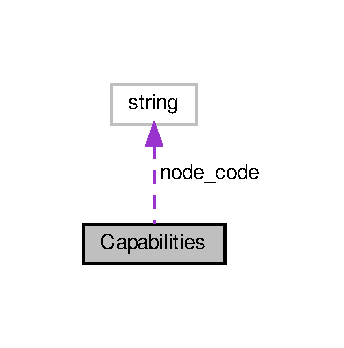
\includegraphics[width=165pt]{structCapabilities__coll__graph}
\end{center}
\end{figure}
\subsection*{Public Member Functions}
\begin{DoxyCompactItemize}
\item 
\mbox{\Hypertarget{structCapabilities_a1a12dfd9ffe75c5bf62b2e5b526cb0d1}\label{structCapabilities_a1a12dfd9ffe75c5bf62b2e5b526cb0d1}} 
void {\bfseries Print\+Capabilities} ()
\item 
\mbox{\Hypertarget{structCapabilities_ab89f31c181ad2ec790b4c7f8dde21609}\label{structCapabilities_ab89f31c181ad2ec790b4c7f8dde21609}} 
void {\bfseries Write\+Capabilities} (\hyperlink{structLogger}{Logger} logger, double sim\+\_\+time)
\item 
void \hyperlink{structCapabilities_a1a12dfd9ffe75c5bf62b2e5b526cb0d1}{Print\+Capabilities} ()
\begin{DoxyCompactList}\small\item\em \begin{quote}
Default modulation \end{quote}
\end{DoxyCompactList}\item 
void \hyperlink{structCapabilities_ab89f31c181ad2ec790b4c7f8dde21609}{Write\+Capabilities} (\hyperlink{structLogger}{Logger} logger, double sim\+\_\+time)
\end{DoxyCompactItemize}
\subsection*{Public Attributes}
\begin{DoxyCompactItemize}
\item 
\mbox{\Hypertarget{structCapabilities_a7edd9b5f5915c8c47b7e0a30ee080c6a}\label{structCapabilities_a7edd9b5f5915c8c47b7e0a30ee080c6a}} 
std\+::string {\bfseries node\+\_\+code}
\item 
\mbox{\Hypertarget{structCapabilities_ac324f6406f7cb8de038c02f1fb24b3d0}\label{structCapabilities_ac324f6406f7cb8de038c02f1fb24b3d0}} 
int \hyperlink{structCapabilities_ac324f6406f7cb8de038c02f1fb24b3d0}{node\+\_\+id}
\begin{DoxyCompactList}\small\item\em \begin{quote}
Node code \end{quote}
\end{DoxyCompactList}\item 
\mbox{\Hypertarget{structCapabilities_a1e7477140acd509bcc68d9afdccdd2fe}\label{structCapabilities_a1e7477140acd509bcc68d9afdccdd2fe}} 
double \hyperlink{structCapabilities_a1e7477140acd509bcc68d9afdccdd2fe}{x}
\begin{DoxyCompactList}\small\item\em \begin{quote}
Node id \end{quote}
\end{DoxyCompactList}\item 
\mbox{\Hypertarget{structCapabilities_a4c7e942cf637661f4f39ba0a979fac6a}\label{structCapabilities_a4c7e942cf637661f4f39ba0a979fac6a}} 
double \hyperlink{structCapabilities_a4c7e942cf637661f4f39ba0a979fac6a}{y}
\begin{DoxyCompactList}\small\item\em \begin{quote}
X position coordinate \end{quote}
\end{DoxyCompactList}\item 
\mbox{\Hypertarget{structCapabilities_af2c88b2fa6b6209c3ee04a5e5c211f5b}\label{structCapabilities_af2c88b2fa6b6209c3ee04a5e5c211f5b}} 
double \hyperlink{structCapabilities_af2c88b2fa6b6209c3ee04a5e5c211f5b}{z}
\begin{DoxyCompactList}\small\item\em \begin{quote}
Y position coordinate \end{quote}
\end{DoxyCompactList}\item 
\mbox{\Hypertarget{structCapabilities_a1193f0213dfc1a0efd15eaf65b0ea45c}\label{structCapabilities_a1193f0213dfc1a0efd15eaf65b0ea45c}} 
int \hyperlink{structCapabilities_a1193f0213dfc1a0efd15eaf65b0ea45c}{node\+\_\+type}
\begin{DoxyCompactList}\small\item\em \begin{quote}
Z position coordinate \end{quote}
\end{DoxyCompactList}\item 
\mbox{\Hypertarget{structCapabilities_ab551c86dab551aa25bd42a5230b456c2}\label{structCapabilities_ab551c86dab551aa25bd42a5230b456c2}} 
int \hyperlink{structCapabilities_ab551c86dab551aa25bd42a5230b456c2}{destination\+\_\+id}
\begin{DoxyCompactList}\small\item\em \begin{quote}
Node type (e.\+g., AP, S\+TA, ...) \end{quote}
\end{DoxyCompactList}\item 
\mbox{\Hypertarget{structCapabilities_a7d819ae08c2d5100ae73976f3ad2026e}\label{structCapabilities_a7d819ae08c2d5100ae73976f3ad2026e}} 
double \hyperlink{structCapabilities_a7d819ae08c2d5100ae73976f3ad2026e}{lambda}
\begin{DoxyCompactList}\small\item\em \begin{quote}
Destination node id (for nodes not belonging to any W\+L\+AN) \end{quote}
\end{DoxyCompactList}\item 
\mbox{\Hypertarget{structCapabilities_a8c1dc96e13e54efefbaed6e0218a4e30}\label{structCapabilities_a8c1dc96e13e54efefbaed6e0218a4e30}} 
double \hyperlink{structCapabilities_a8c1dc96e13e54efefbaed6e0218a4e30}{traffic\+\_\+load}
\begin{DoxyCompactList}\small\item\em \begin{quote}
Average notification generation rate (related to exponential BO) \mbox{[}notification/s\mbox{]} \end{quote}
\end{DoxyCompactList}\item 
\mbox{\Hypertarget{structCapabilities_a619b798b45dc3bfcb0456b663918e534}\label{structCapabilities_a619b798b45dc3bfcb0456b663918e534}} 
int \hyperlink{structCapabilities_a619b798b45dc3bfcb0456b663918e534}{ieee\+\_\+protocol}
\begin{DoxyCompactList}\small\item\em \begin{quote}
Average traffic load of the AP \mbox{[}packets/s\mbox{]} \end{quote}
\end{DoxyCompactList}\item 
\mbox{\Hypertarget{structCapabilities_acef3010e3cc7c8031e00824c20fce068}\label{structCapabilities_acef3010e3cc7c8031e00824c20fce068}} 
int \hyperlink{structCapabilities_acef3010e3cc7c8031e00824c20fce068}{primary\+\_\+channel}
\begin{DoxyCompactList}\small\item\em \begin{quote}
I\+E\+EE protocol type \end{quote}
\end{DoxyCompactList}\item 
\mbox{\Hypertarget{structCapabilities_a5f4060c7db110398fd90c25f13599535}\label{structCapabilities_a5f4060c7db110398fd90c25f13599535}} 
int \hyperlink{structCapabilities_a5f4060c7db110398fd90c25f13599535}{min\+\_\+channel\+\_\+allowed}
\begin{DoxyCompactList}\small\item\em \begin{quote}
Primary channel \end{quote}
\end{DoxyCompactList}\item 
\mbox{\Hypertarget{structCapabilities_ade2db61b6d5cfa458e31b56810a7a7ee}\label{structCapabilities_ade2db61b6d5cfa458e31b56810a7a7ee}} 
int \hyperlink{structCapabilities_ade2db61b6d5cfa458e31b56810a7a7ee}{max\+\_\+channel\+\_\+allowed}
\begin{DoxyCompactList}\small\item\em \begin{quote}
Min. allowed channel \end{quote}
\end{DoxyCompactList}\item 
\mbox{\Hypertarget{structCapabilities_a7bbbcd7bbe2fce0b9d3a3237376759af}\label{structCapabilities_a7bbbcd7bbe2fce0b9d3a3237376759af}} 
int \hyperlink{structCapabilities_a7bbbcd7bbe2fce0b9d3a3237376759af}{num\+\_\+channels\+\_\+allowed}
\begin{DoxyCompactList}\small\item\em \begin{quote}
Max. allowed channel \end{quote}
\end{DoxyCompactList}\item 
\mbox{\Hypertarget{structCapabilities_abda141935667404464ef0a637db1ba2a}\label{structCapabilities_abda141935667404464ef0a637db1ba2a}} 
double \hyperlink{structCapabilities_abda141935667404464ef0a637db1ba2a}{tx\+\_\+power\+\_\+min}
\begin{DoxyCompactList}\small\item\em \begin{quote}
Maximum number of channels allowed to TX in \end{quote}
\end{DoxyCompactList}\item 
\mbox{\Hypertarget{structCapabilities_a1d452f9b15fb03b25d40bb92f455b6b5}\label{structCapabilities_a1d452f9b15fb03b25d40bb92f455b6b5}} 
double \hyperlink{structCapabilities_a1d452f9b15fb03b25d40bb92f455b6b5}{tx\+\_\+power\+\_\+default}
\begin{DoxyCompactList}\small\item\em \begin{quote}
Min. power transmission \mbox{[}pW\mbox{]} \end{quote}
\end{DoxyCompactList}\item 
\mbox{\Hypertarget{structCapabilities_ab8290a1aacc4a64c2c3033bd4ea5034f}\label{structCapabilities_ab8290a1aacc4a64c2c3033bd4ea5034f}} 
double \hyperlink{structCapabilities_ab8290a1aacc4a64c2c3033bd4ea5034f}{tx\+\_\+power\+\_\+max}
\begin{DoxyCompactList}\small\item\em \begin{quote}
Default power transmission \mbox{[}pW\mbox{]} \end{quote}
\end{DoxyCompactList}\item 
\mbox{\Hypertarget{structCapabilities_a4477344b4ebea51cac5b63b14e20d50a}\label{structCapabilities_a4477344b4ebea51cac5b63b14e20d50a}} 
double \hyperlink{structCapabilities_a4477344b4ebea51cac5b63b14e20d50a}{sensitivity\+\_\+min}
\begin{DoxyCompactList}\small\item\em \begin{quote}
Max. power transmission \mbox{[}pW\mbox{]} \end{quote}
\end{DoxyCompactList}\item 
\mbox{\Hypertarget{structCapabilities_a2c5fb9de1c43c79cee6798c016211cb2}\label{structCapabilities_a2c5fb9de1c43c79cee6798c016211cb2}} 
double \hyperlink{structCapabilities_a2c5fb9de1c43c79cee6798c016211cb2}{sensitivity\+\_\+default}
\begin{DoxyCompactList}\small\item\em \begin{quote}
Min. pd (\char`\"{}sensitivity\char`\"{} threshold) \mbox{[}pW\mbox{]} \end{quote}
\end{DoxyCompactList}\item 
\mbox{\Hypertarget{structCapabilities_aee6c344ee3bcd10f43cf0cbc10b2a498}\label{structCapabilities_aee6c344ee3bcd10f43cf0cbc10b2a498}} 
double \hyperlink{structCapabilities_aee6c344ee3bcd10f43cf0cbc10b2a498}{sensitivity\+\_\+max}
\begin{DoxyCompactList}\small\item\em \begin{quote}
Default pd (\char`\"{}sensitivity\char`\"{} threshold) \mbox{[}pW\mbox{]} \end{quote}
\end{DoxyCompactList}\item 
\mbox{\Hypertarget{structCapabilities_a4196e85f00573d428b1e9007331d2ce7}\label{structCapabilities_a4196e85f00573d428b1e9007331d2ce7}} 
double \hyperlink{structCapabilities_a4196e85f00573d428b1e9007331d2ce7}{tx\+\_\+gain}
\begin{DoxyCompactList}\small\item\em \begin{quote}
Max. pd (\char`\"{}sensitivity\char`\"{} threshold) \end{quote}
\end{DoxyCompactList}\item 
\mbox{\Hypertarget{structCapabilities_ad35c7f2ceb255db88cf27b8b09cb24bd}\label{structCapabilities_ad35c7f2ceb255db88cf27b8b09cb24bd}} 
double \hyperlink{structCapabilities_ad35c7f2ceb255db88cf27b8b09cb24bd}{rx\+\_\+gain}
\begin{DoxyCompactList}\small\item\em \begin{quote}
Antenna transmission gain \mbox{[}linear\mbox{]} \end{quote}
\end{DoxyCompactList}\item 
\mbox{\Hypertarget{structCapabilities_ae05428c083582018c872bd8d6da04638}\label{structCapabilities_ae05428c083582018c872bd8d6da04638}} 
int \hyperlink{structCapabilities_ae05428c083582018c872bd8d6da04638}{current\+\_\+dcb\+\_\+policy}
\begin{DoxyCompactList}\small\item\em \begin{quote}
Antenna reception gain \mbox{[}linear\mbox{]} \end{quote}
\end{DoxyCompactList}\item 
\mbox{\Hypertarget{structCapabilities_aed928b77fc111cde1845dc9df3df8696}\label{structCapabilities_aed928b77fc111cde1845dc9df3df8696}} 
int \hyperlink{structCapabilities_aed928b77fc111cde1845dc9df3df8696}{modulation\+\_\+default}
\begin{DoxyCompactList}\small\item\em \begin{quote}
Selected D\+CB policy \end{quote}
\end{DoxyCompactList}\end{DoxyCompactItemize}


\subsection{Detailed Description}
\hyperlink{node__configuration_8h_source}{node\+\_\+configuration.\+h}\+: this file defines a C\+O\+N\+F\+I\+G\+U\+R\+A\+T\+I\+ON and provides basic displaying methods 

\subsection{Member Function Documentation}
\mbox{\Hypertarget{structCapabilities_a1a12dfd9ffe75c5bf62b2e5b526cb0d1}\label{structCapabilities_a1a12dfd9ffe75c5bf62b2e5b526cb0d1}} 
\index{Capabilities@{Capabilities}!Print\+Capabilities@{Print\+Capabilities}}
\index{Print\+Capabilities@{Print\+Capabilities}!Capabilities@{Capabilities}}
\subsubsection{\texorpdfstring{Print\+Capabilities()}{PrintCapabilities()}}
{\footnotesize\ttfamily void Capabilities\+::\+Print\+Capabilities (\begin{DoxyParamCaption}{ }\end{DoxyParamCaption})\hspace{0.3cm}{\ttfamily [inline]}}



\begin{quote}
Default modulation \end{quote}


Function to print the node\textquotesingle{}s capabilities \mbox{\Hypertarget{structCapabilities_ab89f31c181ad2ec790b4c7f8dde21609}\label{structCapabilities_ab89f31c181ad2ec790b4c7f8dde21609}} 
\index{Capabilities@{Capabilities}!Write\+Capabilities@{Write\+Capabilities}}
\index{Write\+Capabilities@{Write\+Capabilities}!Capabilities@{Capabilities}}
\subsubsection{\texorpdfstring{Write\+Capabilities()}{WriteCapabilities()}}
{\footnotesize\ttfamily void Capabilities\+::\+Write\+Capabilities (\begin{DoxyParamCaption}\item[{\hyperlink{structLogger}{Logger}}]{logger,  }\item[{double}]{sim\+\_\+time }\end{DoxyParamCaption})\hspace{0.3cm}{\ttfamily [inline]}}

Function to write the node\textquotesingle{}s capabilities 
\begin{DoxyParams}{Parameters}
{\em logger} & \mbox{[}type \hyperlink{structLogger}{Logger}\mbox{]}\+: logger object for printing logs into a file \\
\hline
{\em sim\+\_\+time} & \mbox{[}type double\mbox{]}\+: current simulation time \\
\hline
\end{DoxyParams}


The documentation for this struct was generated from the following files\+:\begin{DoxyCompactItemize}
\item 
Code/main/komondor\+\_\+main.\+cxx\item 
Code/structures/node\+\_\+configuration.\+h\end{DoxyCompactItemize}

\hypertarget{structether__addr__t_1_1compare}{}\section{ether\+\_\+addr\+\_\+t\+:\+:compare Struct Reference}
\label{structether__addr__t_1_1compare}\index{ether\+\_\+addr\+\_\+t\+::compare@{ether\+\_\+addr\+\_\+t\+::compare}}
\subsection*{Public Member Functions}
\begin{DoxyCompactItemize}
\item 
\mbox{\Hypertarget{structether__addr__t_1_1compare_a5d406d61bb2102903fc8ed7d56fb9c96}\label{structether__addr__t_1_1compare_a5d406d61bb2102903fc8ed7d56fb9c96}} 
bool {\bfseries operator()} (const \hyperlink{classether__addr__t}{ether\+\_\+addr\+\_\+t} \&e1, const \hyperlink{classether__addr__t}{ether\+\_\+addr\+\_\+t} \&e2)
\end{DoxyCompactItemize}


The documentation for this struct was generated from the following file\+:\begin{DoxyCompactItemize}
\item 
Code/\+C\+O\+S\+T/ether\+\_\+addr.\+h\end{DoxyCompactItemize}

\hypertarget{classcompcxx__Agent__25}{}\section{compcxx\+\_\+\+Agent\+\_\+25 Class Reference}
\label{classcompcxx__Agent__25}\index{compcxx\+\_\+\+Agent\+\_\+25@{compcxx\+\_\+\+Agent\+\_\+25}}


Inheritance diagram for compcxx\+\_\+\+Agent\+\_\+25\+:\nopagebreak
\begin{figure}[H]
\begin{center}
\leavevmode
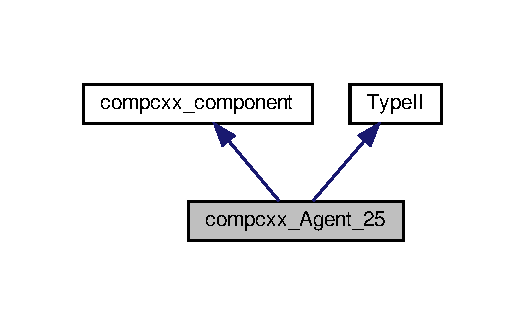
\includegraphics[width=252pt]{classcompcxx__Agent__25__inherit__graph}
\end{center}
\end{figure}


Collaboration diagram for compcxx\+\_\+\+Agent\+\_\+25\+:\nopagebreak
\begin{figure}[H]
\begin{center}
\leavevmode
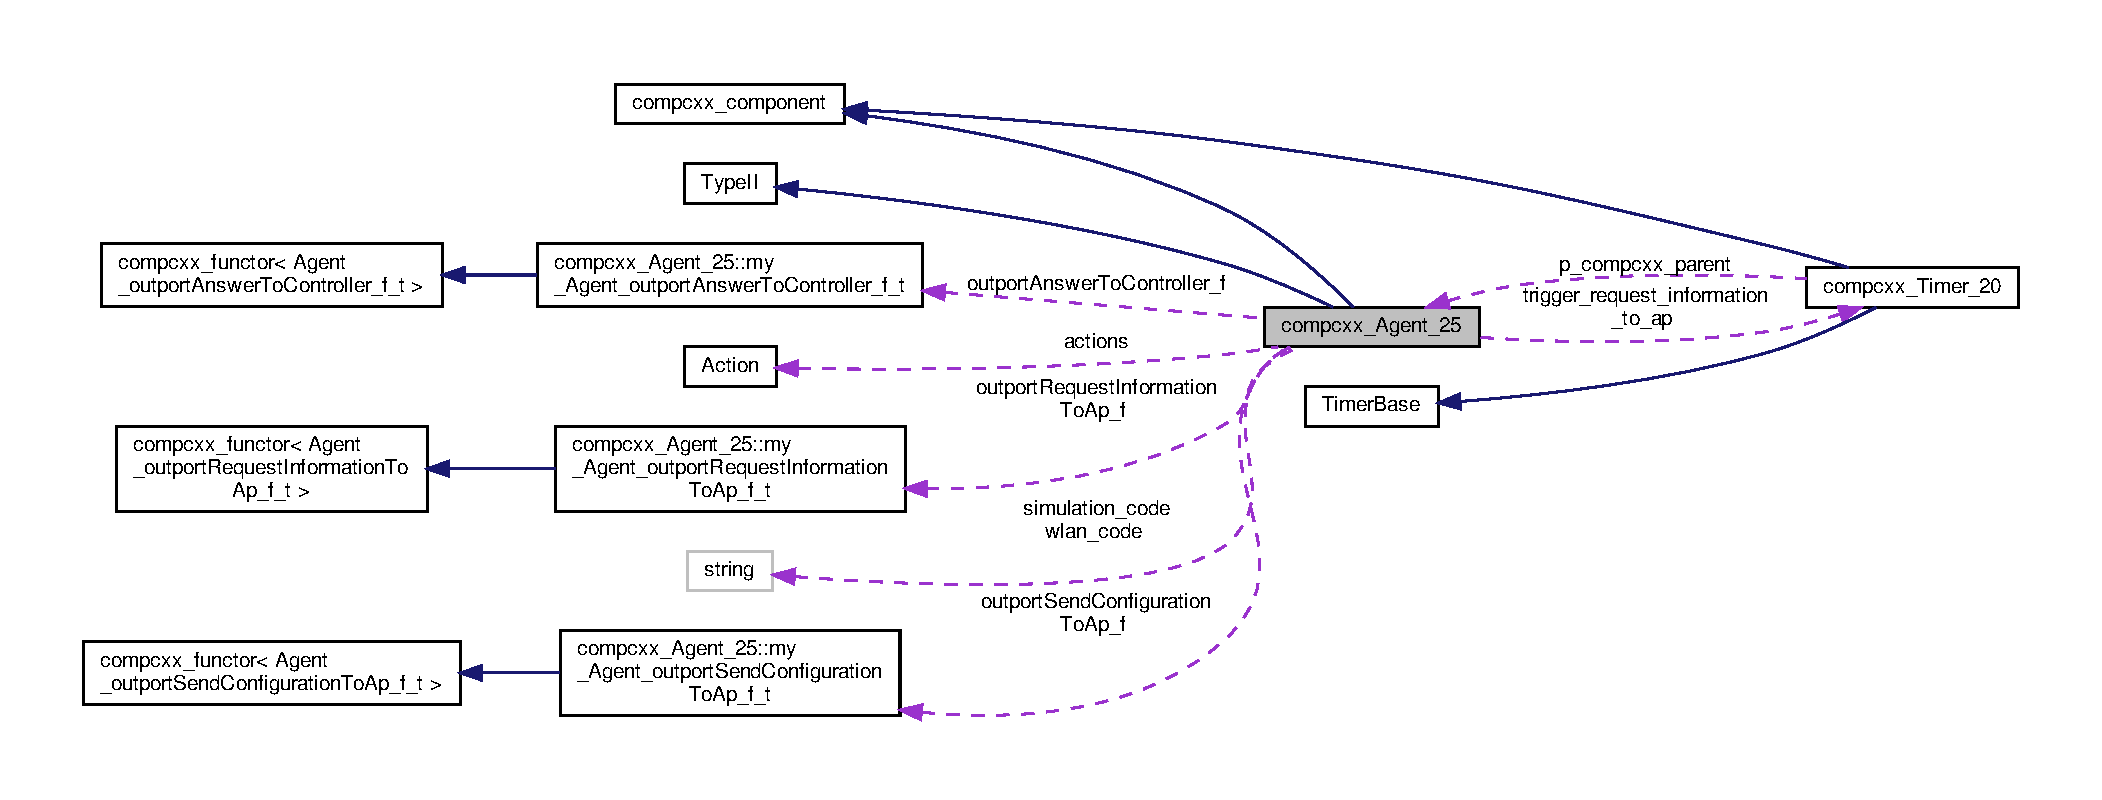
\includegraphics[width=350pt]{classcompcxx__Agent__25__coll__graph}
\end{center}
\end{figure}
\subsection*{Classes}
\begin{DoxyCompactItemize}
\item 
class \hyperlink{classcompcxx__Agent__25_1_1my__Agent__outportAnswerToController__f__t}{my\+\_\+\+Agent\+\_\+outport\+Answer\+To\+Controller\+\_\+f\+\_\+t}
\item 
class \hyperlink{classcompcxx__Agent__25_1_1my__Agent__outportRequestInformationToAp__f__t}{my\+\_\+\+Agent\+\_\+outport\+Request\+Information\+To\+Ap\+\_\+f\+\_\+t}
\item 
class \hyperlink{classcompcxx__Agent__25_1_1my__Agent__outportSendConfigurationToAp__f__t}{my\+\_\+\+Agent\+\_\+outport\+Send\+Configuration\+To\+Ap\+\_\+f\+\_\+t}
\end{DoxyCompactItemize}
\subsection*{Public Member Functions}
\begin{DoxyCompactItemize}
\item 
\mbox{\Hypertarget{classcompcxx__Agent__25_a3ec14b5b6a2cd192de9b2ce367f3f6d9}\label{classcompcxx__Agent__25_a3ec14b5b6a2cd192de9b2ce367f3f6d9}} 
void {\bfseries Setup} ()
\item 
\mbox{\Hypertarget{classcompcxx__Agent__25_a6f110202e6343a30b286f3c1ab7f056c}\label{classcompcxx__Agent__25_a6f110202e6343a30b286f3c1ab7f056c}} 
void {\bfseries Start} ()
\item 
\mbox{\Hypertarget{classcompcxx__Agent__25_a5b97e82bc95b4a40a1ac771e5aa828f0}\label{classcompcxx__Agent__25_a5b97e82bc95b4a40a1ac771e5aa828f0}} 
void {\bfseries Stop} ()
\item 
\mbox{\Hypertarget{classcompcxx__Agent__25_a063e3f7f45e930741172376b26e3e748}\label{classcompcxx__Agent__25_a063e3f7f45e930741172376b26e3e748}} 
void {\bfseries Initialize\+Agent} ()
\item 
\mbox{\Hypertarget{classcompcxx__Agent__25_ac6892ce3eef81f340d30bb58a0d4b393}\label{classcompcxx__Agent__25_ac6892ce3eef81f340d30bb58a0d4b393}} 
void {\bfseries Initialize\+Pre\+Processor} ()
\item 
\mbox{\Hypertarget{classcompcxx__Agent__25_ae732e92ffff2bc34d93c15d77fb23b97}\label{classcompcxx__Agent__25_ae732e92ffff2bc34d93c15d77fb23b97}} 
void {\bfseries Initialize\+Ml\+Model} ()
\item 
\mbox{\Hypertarget{classcompcxx__Agent__25_ad8d476c02b12c6f216d309be2f0716bc}\label{classcompcxx__Agent__25_ad8d476c02b12c6f216d309be2f0716bc}} 
void {\bfseries Request\+Information\+To\+Ap} ()
\item 
\mbox{\Hypertarget{classcompcxx__Agent__25_a3bf9618e57b14c8f3301bc1ce9f127b0}\label{classcompcxx__Agent__25_a3bf9618e57b14c8f3301bc1ce9f127b0}} 
void {\bfseries Compute\+New\+Configuration} ()
\item 
\mbox{\Hypertarget{classcompcxx__Agent__25_a68025881fe2f2f5a908b471810885dee}\label{classcompcxx__Agent__25_a68025881fe2f2f5a908b471810885dee}} 
void {\bfseries Send\+New\+Configuration\+To\+Ap} (\hyperlink{structConfiguration}{Configuration} \&configuration\+\_\+to\+\_\+send)
\item 
\mbox{\Hypertarget{classcompcxx__Agent__25_ac0b2cfb425ed43ae5ff4e603e69addd7}\label{classcompcxx__Agent__25_ac0b2cfb425ed43ae5ff4e603e69addd7}} 
void {\bfseries Print\+Agent\+Info} ()
\item 
\mbox{\Hypertarget{classcompcxx__Agent__25_a90951f40579a12cb4b5584acbf7eedb8}\label{classcompcxx__Agent__25_a90951f40579a12cb4b5584acbf7eedb8}} 
void {\bfseries Write\+Agent\+Info} (\hyperlink{structLogger}{Logger} logger, std\+::string header\+\_\+str)
\item 
\mbox{\Hypertarget{classcompcxx__Agent__25_a504a6b195024a6533a35954c20e02b61}\label{classcompcxx__Agent__25_a504a6b195024a6533a35954c20e02b61}} 
void {\bfseries Write\+Configuration} (\hyperlink{structConfiguration}{Configuration} configuration\+\_\+to\+\_\+write)
\item 
\mbox{\Hypertarget{classcompcxx__Agent__25_a628b28322f02142603257b83b860c7de}\label{classcompcxx__Agent__25_a628b28322f02142603257b83b860c7de}} 
void {\bfseries Write\+Performance} (\hyperlink{structPerformance}{Performance} performance\+\_\+to\+\_\+write)
\item 
\mbox{\Hypertarget{classcompcxx__Agent__25_a2816c04a03b20a1d296355d5fe3674f4}\label{classcompcxx__Agent__25_a2816c04a03b20a1d296355d5fe3674f4}} 
void {\bfseries Print\+Or\+Write\+Agent\+Statistics} ()
\item 
\mbox{\Hypertarget{classcompcxx__Agent__25_ada9e8f711e760739d00ae2cfe3a95c7e}\label{classcompcxx__Agent__25_ada9e8f711e760739d00ae2cfe3a95c7e}} 
void {\bfseries Inport\+Receiving\+Information\+From\+Ap} (\hyperlink{structConfiguration}{Configuration} \&configuration, \hyperlink{structPerformance}{Performance} \&performance)
\item 
\mbox{\Hypertarget{classcompcxx__Agent__25_a0304719f509dbc5031e6f718c1b6a7ee}\label{classcompcxx__Agent__25_a0304719f509dbc5031e6f718c1b6a7ee}} 
void {\bfseries Inport\+Receiving\+Request\+From\+Controller} (int destination\+\_\+agent\+\_\+id)
\item 
\mbox{\Hypertarget{classcompcxx__Agent__25_a314c2ae1f9dbbc04232c6b50aa10f836}\label{classcompcxx__Agent__25_a314c2ae1f9dbbc04232c6b50aa10f836}} 
void {\bfseries Inport\+Receive\+Configuration\+From\+Controller} (int destination\+\_\+agent\+\_\+id, \hyperlink{structConfiguration}{Configuration} \&new\+\_\+configuration, int controller\+\_\+mode)
\item 
\mbox{\Hypertarget{classcompcxx__Agent__25_a4a7b7f09914ec79562dfa2768a7888a6}\label{classcompcxx__Agent__25_a4a7b7f09914ec79562dfa2768a7888a6}} 
void {\bfseries Request\+Information\+To\+Ap} (\hyperlink{classtrigger__t}{trigger\+\_\+t} \&t1)
\end{DoxyCompactItemize}
\subsection*{Public Attributes}
\begin{DoxyCompactItemize}
\item 
\mbox{\Hypertarget{classcompcxx__Agent__25_ae8e1db9b24fb88d3e1db47d8bd4c3231}\label{classcompcxx__Agent__25_ae8e1db9b24fb88d3e1db47d8bd4c3231}} 
int {\bfseries agent\+\_\+id}
\item 
\mbox{\Hypertarget{classcompcxx__Agent__25_a223a23208341b7817c96503e9131a3a8}\label{classcompcxx__Agent__25_a223a23208341b7817c96503e9131a3a8}} 
int {\bfseries communication\+\_\+level}
\item 
\mbox{\Hypertarget{classcompcxx__Agent__25_a67b4ca9a2d5b2da2a7da930f844aa8d1}\label{classcompcxx__Agent__25_a67b4ca9a2d5b2da2a7da930f844aa8d1}} 
std\+::string {\bfseries wlan\+\_\+code}
\item 
\mbox{\Hypertarget{classcompcxx__Agent__25_af5a59b1e7a2a0756c836a858545b1817}\label{classcompcxx__Agent__25_af5a59b1e7a2a0756c836a858545b1817}} 
int {\bfseries learning\+\_\+mechanism}
\item 
\mbox{\Hypertarget{classcompcxx__Agent__25_aba3264a9879f081771b05e698a533fe0}\label{classcompcxx__Agent__25_aba3264a9879f081771b05e698a533fe0}} 
int {\bfseries action\+\_\+selection\+\_\+strategy}
\item 
\mbox{\Hypertarget{classcompcxx__Agent__25_a5e2e26f3b35e5d4f479f7b0b157b84df}\label{classcompcxx__Agent__25_a5e2e26f3b35e5d4f479f7b0b157b84df}} 
int $\ast$ {\bfseries list\+\_\+of\+\_\+channels}
\item 
\mbox{\Hypertarget{classcompcxx__Agent__25_a3311d54a153af5b6bd49b552e016bb06}\label{classcompcxx__Agent__25_a3311d54a153af5b6bd49b552e016bb06}} 
double $\ast$ {\bfseries list\+\_\+of\+\_\+pd\+\_\+values}
\item 
\mbox{\Hypertarget{classcompcxx__Agent__25_adcd2de310a6fb45a627d43248aace259}\label{classcompcxx__Agent__25_adcd2de310a6fb45a627d43248aace259}} 
double $\ast$ {\bfseries list\+\_\+of\+\_\+tx\+\_\+power\+\_\+values}
\item 
\mbox{\Hypertarget{classcompcxx__Agent__25_a95e687635164fcbc7d61238d762f08c7}\label{classcompcxx__Agent__25_a95e687635164fcbc7d61238d762f08c7}} 
int $\ast$ {\bfseries list\+\_\+of\+\_\+dcb\+\_\+policy}
\item 
\mbox{\Hypertarget{classcompcxx__Agent__25_adb8f34e67c5003fbd77009d235516600}\label{classcompcxx__Agent__25_adb8f34e67c5003fbd77009d235516600}} 
\hyperlink{structAction}{Action} $\ast$ {\bfseries actions}
\item 
\mbox{\Hypertarget{classcompcxx__Agent__25_a7cf530cb0215d06c543ea6362b9de3b1}\label{classcompcxx__Agent__25_a7cf530cb0215d06c543ea6362b9de3b1}} 
int {\bfseries num\+\_\+actions\+\_\+channel}
\item 
\mbox{\Hypertarget{classcompcxx__Agent__25_a6da40f193f5cd6e20ebfb7ef92ffeae9}\label{classcompcxx__Agent__25_a6da40f193f5cd6e20ebfb7ef92ffeae9}} 
int {\bfseries num\+\_\+actions\+\_\+sensitivity}
\item 
\mbox{\Hypertarget{classcompcxx__Agent__25_a4c267340f0dd3332bf625ff80d156ffc}\label{classcompcxx__Agent__25_a4c267340f0dd3332bf625ff80d156ffc}} 
int {\bfseries num\+\_\+actions\+\_\+tx\+\_\+power}
\item 
\mbox{\Hypertarget{classcompcxx__Agent__25_a8eec5256c73aefc2b0fbc93d87ee4034}\label{classcompcxx__Agent__25_a8eec5256c73aefc2b0fbc93d87ee4034}} 
int {\bfseries num\+\_\+actions\+\_\+dcb\+\_\+policy}
\item 
\mbox{\Hypertarget{classcompcxx__Agent__25_a2c59ff7d8f0218a023a3d643878998bf}\label{classcompcxx__Agent__25_a2c59ff7d8f0218a023a3d643878998bf}} 
int {\bfseries type\+\_\+of\+\_\+reward}
\item 
\mbox{\Hypertarget{classcompcxx__Agent__25_a1696b03bde44c35366b42c042f429548}\label{classcompcxx__Agent__25_a1696b03bde44c35366b42c042f429548}} 
double {\bfseries time\+\_\+between\+\_\+requests}
\item 
\mbox{\Hypertarget{classcompcxx__Agent__25_acd0cdd7c585fcf095911fa918ba685d7}\label{classcompcxx__Agent__25_acd0cdd7c585fcf095911fa918ba685d7}} 
int {\bfseries save\+\_\+agent\+\_\+logs}
\item 
\mbox{\Hypertarget{classcompcxx__Agent__25_ac8ab464ff53c21626fcc571ebd88b96b}\label{classcompcxx__Agent__25_ac8ab464ff53c21626fcc571ebd88b96b}} 
int {\bfseries print\+\_\+agent\+\_\+logs}
\item 
\mbox{\Hypertarget{classcompcxx__Agent__25_a9d7353ccb286cf911420534676bfcd19}\label{classcompcxx__Agent__25_a9d7353ccb286cf911420534676bfcd19}} 
std\+::string {\bfseries simulation\+\_\+code}
\item 
\mbox{\Hypertarget{classcompcxx__Agent__25_a7d9935510c1c0a234d498e50fe6b19c5}\label{classcompcxx__Agent__25_a7d9935510c1c0a234d498e50fe6b19c5}} 
\hyperlink{classcompcxx__Agent__25_1_1my__Agent__outportRequestInformationToAp__f__t}{my\+\_\+\+Agent\+\_\+outport\+Request\+Information\+To\+Ap\+\_\+f\+\_\+t} {\bfseries outport\+Request\+Information\+To\+Ap\+\_\+f}
\item 
\mbox{\Hypertarget{classcompcxx__Agent__25_abe7d79ae04ff57646e7d29030f8a36c2}\label{classcompcxx__Agent__25_abe7d79ae04ff57646e7d29030f8a36c2}} 
\hyperlink{classcompcxx__Agent__25_1_1my__Agent__outportSendConfigurationToAp__f__t}{my\+\_\+\+Agent\+\_\+outport\+Send\+Configuration\+To\+Ap\+\_\+f\+\_\+t} {\bfseries outport\+Send\+Configuration\+To\+Ap\+\_\+f}
\item 
\mbox{\Hypertarget{classcompcxx__Agent__25_ab5641f447eebe576ae65136ab8229712}\label{classcompcxx__Agent__25_ab5641f447eebe576ae65136ab8229712}} 
\hyperlink{classcompcxx__Agent__25_1_1my__Agent__outportAnswerToController__f__t}{my\+\_\+\+Agent\+\_\+outport\+Answer\+To\+Controller\+\_\+f\+\_\+t} {\bfseries outport\+Answer\+To\+Controller\+\_\+f}
\item 
\mbox{\Hypertarget{classcompcxx__Agent__25_a662cb6f32dac818e3a215f9cb4a9f73d}\label{classcompcxx__Agent__25_a662cb6f32dac818e3a215f9cb4a9f73d}} 
\hyperlink{classcompcxx__Timer__20}{compcxx\+\_\+\+Timer\+\_\+20} {\bfseries trigger\+\_\+request\+\_\+information\+\_\+to\+\_\+ap}
\end{DoxyCompactItemize}
\subsection*{Additional Inherited Members}


The documentation for this class was generated from the following file\+:\begin{DoxyCompactItemize}
\item 
Code/main/komondor\+\_\+main.\+cxx\end{DoxyCompactItemize}

\hypertarget{classcompcxx__array}{}\section{compcxx\+\_\+array$<$ T $>$ Class Template Reference}
\label{classcompcxx__array}\index{compcxx\+\_\+array$<$ T $>$@{compcxx\+\_\+array$<$ T $>$}}
\subsection*{Public Member Functions}
\begin{DoxyCompactItemize}
\item 
\mbox{\Hypertarget{classcompcxx__array_a873f82aa570a68fd38046f8f8dfc7f99}\label{classcompcxx__array_a873f82aa570a68fd38046f8f8dfc7f99}} 
void {\bfseries Set\+Size} (unsigned int n)
\item 
\mbox{\Hypertarget{classcompcxx__array_a26b1d1297b95f557aeca69f390afa521}\label{classcompcxx__array_a26b1d1297b95f557aeca69f390afa521}} 
T \& {\bfseries operator\mbox{[}$\,$\mbox{]}} (unsigned int i)
\item 
\mbox{\Hypertarget{classcompcxx__array_a05fdecc7552fdb939f217fcc46e50cf4}\label{classcompcxx__array_a05fdecc7552fdb939f217fcc46e50cf4}} 
unsigned int {\bfseries size} ()
\end{DoxyCompactItemize}


The documentation for this class was generated from the following file\+:\begin{DoxyCompactItemize}
\item 
Code/main/compcxx\+\_\+komondor\+\_\+main.\+h\end{DoxyCompactItemize}

\hypertarget{classcompcxx__CentralController__26}{}\section{compcxx\+\_\+\+Central\+Controller\+\_\+26 Class Reference}
\label{classcompcxx__CentralController__26}\index{compcxx\+\_\+\+Central\+Controller\+\_\+26@{compcxx\+\_\+\+Central\+Controller\+\_\+26}}


Inheritance diagram for compcxx\+\_\+\+Central\+Controller\+\_\+26\+:\nopagebreak
\begin{figure}[H]
\begin{center}
\leavevmode
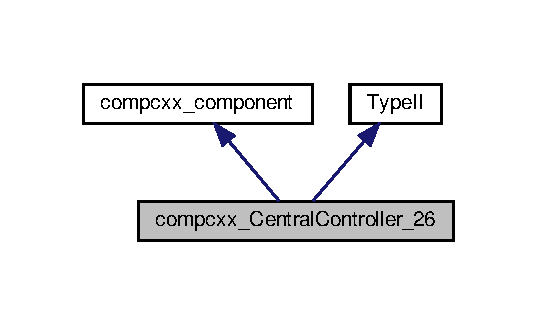
\includegraphics[width=258pt]{classcompcxx__CentralController__26__inherit__graph}
\end{center}
\end{figure}


Collaboration diagram for compcxx\+\_\+\+Central\+Controller\+\_\+26\+:\nopagebreak
\begin{figure}[H]
\begin{center}
\leavevmode
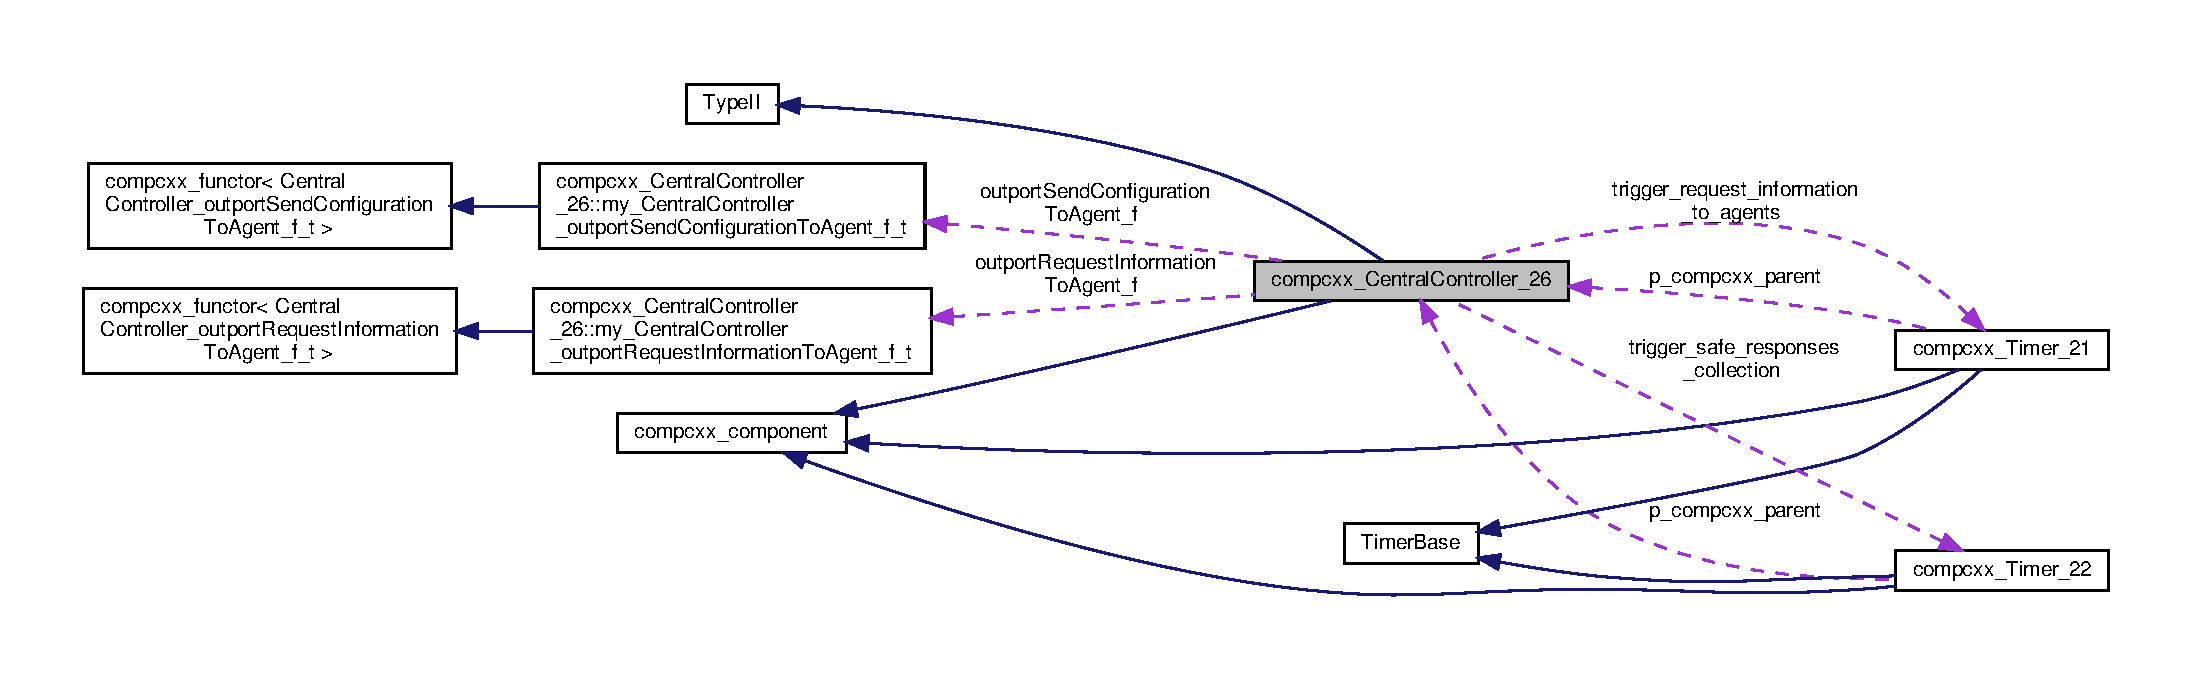
\includegraphics[width=350pt]{classcompcxx__CentralController__26__coll__graph}
\end{center}
\end{figure}
\subsection*{Classes}
\begin{DoxyCompactItemize}
\item 
class \hyperlink{classcompcxx__CentralController__26_1_1my__CentralController__outportRequestInformationToAgent__f__t}{my\+\_\+\+Central\+Controller\+\_\+outport\+Request\+Information\+To\+Agent\+\_\+f\+\_\+t}
\item 
class \hyperlink{classcompcxx__CentralController__26_1_1my__CentralController__outportSendConfigurationToAgent__f__t}{my\+\_\+\+Central\+Controller\+\_\+outport\+Send\+Configuration\+To\+Agent\+\_\+f\+\_\+t}
\end{DoxyCompactItemize}
\subsection*{Public Member Functions}
\begin{DoxyCompactItemize}
\item 
\mbox{\Hypertarget{classcompcxx__CentralController__26_af502b2d53c56b98819b90701177786b6}\label{classcompcxx__CentralController__26_af502b2d53c56b98819b90701177786b6}} 
void {\bfseries Setup} ()
\item 
\mbox{\Hypertarget{classcompcxx__CentralController__26_a6e310ea47cfd87befacac15ad20b5ed7}\label{classcompcxx__CentralController__26_a6e310ea47cfd87befacac15ad20b5ed7}} 
void {\bfseries Start} ()
\item 
\mbox{\Hypertarget{classcompcxx__CentralController__26_aee7d621f5e9505dbbf90954b5fe5ff20}\label{classcompcxx__CentralController__26_aee7d621f5e9505dbbf90954b5fe5ff20}} 
void {\bfseries Stop} ()
\item 
\mbox{\Hypertarget{classcompcxx__CentralController__26_ada0b5a8f856377a4f274710d922988c8}\label{classcompcxx__CentralController__26_ada0b5a8f856377a4f274710d922988c8}} 
void {\bfseries Initialize\+Central\+Controller} ()
\item 
\mbox{\Hypertarget{classcompcxx__CentralController__26_af394845a8af7930c03120338b4906e87}\label{classcompcxx__CentralController__26_af394845a8af7930c03120338b4906e87}} 
void {\bfseries Request\+Information\+To\+Agents} ()
\item 
\mbox{\Hypertarget{classcompcxx__CentralController__26_abfb6f274083e445d3d3e8a8ad6b5b55a}\label{classcompcxx__CentralController__26_abfb6f274083e445d3d3e8a8ad6b5b55a}} 
void {\bfseries Generate\+And\+Send\+New\+Configuration} ()
\item 
\mbox{\Hypertarget{classcompcxx__CentralController__26_af65e589792a448d316d87eaf2eb283b4}\label{classcompcxx__CentralController__26_af65e589792a448d316d87eaf2eb283b4}} 
void {\bfseries Send\+Configuration\+To\+All\+Agents} ()
\item 
\mbox{\Hypertarget{classcompcxx__CentralController__26_a0e9b6ebd2c775d98f442b3e50d4d09b1}\label{classcompcxx__CentralController__26_a0e9b6ebd2c775d98f442b3e50d4d09b1}} 
void {\bfseries Send\+Configuration\+To\+Single\+Agent} (int destination\+\_\+agent\+\_\+id, \hyperlink{structConfiguration}{Configuration} conf)
\item 
\mbox{\Hypertarget{classcompcxx__CentralController__26_af1257d2a942a1cebad8fff3ea878a35f}\label{classcompcxx__CentralController__26_af1257d2a942a1cebad8fff3ea878a35f}} 
void {\bfseries Print\+Controller\+Info} ()
\item 
\mbox{\Hypertarget{classcompcxx__CentralController__26_a435e72555f967529c864d27f56cad784}\label{classcompcxx__CentralController__26_a435e72555f967529c864d27f56cad784}} 
void {\bfseries Write\+Controller\+Info} (\hyperlink{structLogger}{Logger} logger)
\item 
\mbox{\Hypertarget{classcompcxx__CentralController__26_ab4ecf9884160ee09400d6558280e7745}\label{classcompcxx__CentralController__26_ab4ecf9884160ee09400d6558280e7745}} 
void {\bfseries Print\+Or\+Write\+Controller\+Statistics} (int print\+\_\+or\+\_\+write)
\item 
\mbox{\Hypertarget{classcompcxx__CentralController__26_ab1f4d23d3e2bacc1e3a8c366a319e5a1}\label{classcompcxx__CentralController__26_ab1f4d23d3e2bacc1e3a8c366a319e5a1}} 
void {\bfseries Initialize\+Pre\+Processor} ()
\item 
\mbox{\Hypertarget{classcompcxx__CentralController__26_a5898f87c98328150b3068339fad1a60f}\label{classcompcxx__CentralController__26_a5898f87c98328150b3068339fad1a60f}} 
void {\bfseries Initialize\+Ml\+Model} ()
\item 
\mbox{\Hypertarget{classcompcxx__CentralController__26_a16c6d188ca224758ad784079c74ae7b8}\label{classcompcxx__CentralController__26_a16c6d188ca224758ad784079c74ae7b8}} 
void {\bfseries Inport\+Receiving\+Information\+From\+Agent} (\hyperlink{structConfiguration}{Configuration} \&configuration, \hyperlink{structPerformance}{Performance} \&performance, int agent\+\_\+id)
\item 
\mbox{\Hypertarget{classcompcxx__CentralController__26_ab8a6dc5fa163095aa0c734bf8164e142}\label{classcompcxx__CentralController__26_ab8a6dc5fa163095aa0c734bf8164e142}} 
void {\bfseries Request\+Information\+To\+Agents} (\hyperlink{classtrigger__t}{trigger\+\_\+t} \&t1)
\item 
\mbox{\Hypertarget{classcompcxx__CentralController__26_adbb033d225b0b25007e170216ffc322d}\label{classcompcxx__CentralController__26_adbb033d225b0b25007e170216ffc322d}} 
void {\bfseries Generate\+And\+Send\+New\+Configuration} (\hyperlink{classtrigger__t}{trigger\+\_\+t} \&t1)
\end{DoxyCompactItemize}
\subsection*{Public Attributes}
\begin{DoxyCompactItemize}
\item 
\mbox{\Hypertarget{classcompcxx__CentralController__26_a53a9c3fbea36b98362ca1d21cba5df4a}\label{classcompcxx__CentralController__26_a53a9c3fbea36b98362ca1d21cba5df4a}} 
int {\bfseries agents\+\_\+number}
\item 
\mbox{\Hypertarget{classcompcxx__CentralController__26_a625f6faa8baa03607a022741fe892809}\label{classcompcxx__CentralController__26_a625f6faa8baa03607a022741fe892809}} 
int $\ast$ {\bfseries list\+\_\+of\+\_\+agents}
\item 
\mbox{\Hypertarget{classcompcxx__CentralController__26_ad15dc76fdbd00bc7fe74145a96a13190}\label{classcompcxx__CentralController__26_ad15dc76fdbd00bc7fe74145a96a13190}} 
int {\bfseries wlans\+\_\+number}
\item 
\mbox{\Hypertarget{classcompcxx__CentralController__26_af0eed89b49adbd1977a7d0f98bcb0339}\label{classcompcxx__CentralController__26_af0eed89b49adbd1977a7d0f98bcb0339}} 
int $\ast$ {\bfseries num\+\_\+requests}
\item 
\mbox{\Hypertarget{classcompcxx__CentralController__26_a7edd3d874041206ddf5f29dc206f9547}\label{classcompcxx__CentralController__26_a7edd3d874041206ddf5f29dc206f9547}} 
double {\bfseries time\+\_\+between\+\_\+requests}
\item 
\mbox{\Hypertarget{classcompcxx__CentralController__26_a869a62f5fbed5dc49a0645b7a193519f}\label{classcompcxx__CentralController__26_a869a62f5fbed5dc49a0645b7a193519f}} 
int {\bfseries save\+\_\+controller\+\_\+logs}
\item 
\mbox{\Hypertarget{classcompcxx__CentralController__26_a4703eafb59dc163c8db359712ed2baf6}\label{classcompcxx__CentralController__26_a4703eafb59dc163c8db359712ed2baf6}} 
int {\bfseries print\+\_\+controller\+\_\+logs}
\item 
\mbox{\Hypertarget{classcompcxx__CentralController__26_a2a6c764a06905108e88a3df63647aff9}\label{classcompcxx__CentralController__26_a2a6c764a06905108e88a3df63647aff9}} 
int {\bfseries controller\+\_\+mode}
\item 
\mbox{\Hypertarget{classcompcxx__CentralController__26_a570a7528b975be04b11df8064c75d52c}\label{classcompcxx__CentralController__26_a570a7528b975be04b11df8064c75d52c}} 
int {\bfseries type\+\_\+of\+\_\+reward}
\item 
\mbox{\Hypertarget{classcompcxx__CentralController__26_adadb126e210ad589f1b64c9839d8616d}\label{classcompcxx__CentralController__26_adadb126e210ad589f1b64c9839d8616d}} 
int {\bfseries learning\+\_\+mechanism}
\item 
\mbox{\Hypertarget{classcompcxx__CentralController__26_ab10780d9882b38a15eb7bdc68ba169cb}\label{classcompcxx__CentralController__26_ab10780d9882b38a15eb7bdc68ba169cb}} 
int {\bfseries action\+\_\+selection\+\_\+strategy}
\item 
\mbox{\Hypertarget{classcompcxx__CentralController__26_ad708e1cd02f1e52bd72d95bd26208c82}\label{classcompcxx__CentralController__26_ad708e1cd02f1e52bd72d95bd26208c82}} 
int {\bfseries num\+\_\+channels}
\item 
\mbox{\Hypertarget{classcompcxx__CentralController__26_aaa8c2de9e01045ba5f40b09cd255905f}\label{classcompcxx__CentralController__26_aaa8c2de9e01045ba5f40b09cd255905f}} 
int {\bfseries total\+\_\+nodes\+\_\+number}
\item 
\mbox{\Hypertarget{classcompcxx__CentralController__26_a96fc4d5ef71d1b7522b9fc3daf26b5f3}\label{classcompcxx__CentralController__26_a96fc4d5ef71d1b7522b9fc3daf26b5f3}} 
\hyperlink{classcompcxx__CentralController__26_1_1my__CentralController__outportRequestInformationToAgent__f__t}{my\+\_\+\+Central\+Controller\+\_\+outport\+Request\+Information\+To\+Agent\+\_\+f\+\_\+t} {\bfseries outport\+Request\+Information\+To\+Agent\+\_\+f}
\item 
\mbox{\Hypertarget{classcompcxx__CentralController__26_ad83020a62cb3ce10ab720906d682c5b9}\label{classcompcxx__CentralController__26_ad83020a62cb3ce10ab720906d682c5b9}} 
\hyperlink{classcompcxx__CentralController__26_1_1my__CentralController__outportSendConfigurationToAgent__f__t}{my\+\_\+\+Central\+Controller\+\_\+outport\+Send\+Configuration\+To\+Agent\+\_\+f\+\_\+t} {\bfseries outport\+Send\+Configuration\+To\+Agent\+\_\+f}
\item 
\mbox{\Hypertarget{classcompcxx__CentralController__26_a3f6745ae9e9b3a409cdf0d21cbbdd7fd}\label{classcompcxx__CentralController__26_a3f6745ae9e9b3a409cdf0d21cbbdd7fd}} 
\hyperlink{classcompcxx__Timer__21}{compcxx\+\_\+\+Timer\+\_\+21} {\bfseries trigger\+\_\+request\+\_\+information\+\_\+to\+\_\+agents}
\item 
\mbox{\Hypertarget{classcompcxx__CentralController__26_a98598f16c69b2c0fd885d02dd56a025c}\label{classcompcxx__CentralController__26_a98598f16c69b2c0fd885d02dd56a025c}} 
\hyperlink{classcompcxx__Timer__22}{compcxx\+\_\+\+Timer\+\_\+22} {\bfseries trigger\+\_\+safe\+\_\+responses\+\_\+collection}
\end{DoxyCompactItemize}
\subsection*{Additional Inherited Members}


The documentation for this class was generated from the following file\+:\begin{DoxyCompactItemize}
\item 
Code/main/komondor\+\_\+main.\+cxx\end{DoxyCompactItemize}

\hypertarget{classcompcxx__component}{}\section{compcxx\+\_\+component Class Reference}
\label{classcompcxx__component}\index{compcxx\+\_\+component@{compcxx\+\_\+component}}


Inheritance diagram for compcxx\+\_\+component\+:\nopagebreak
\begin{figure}[H]
\begin{center}
\leavevmode
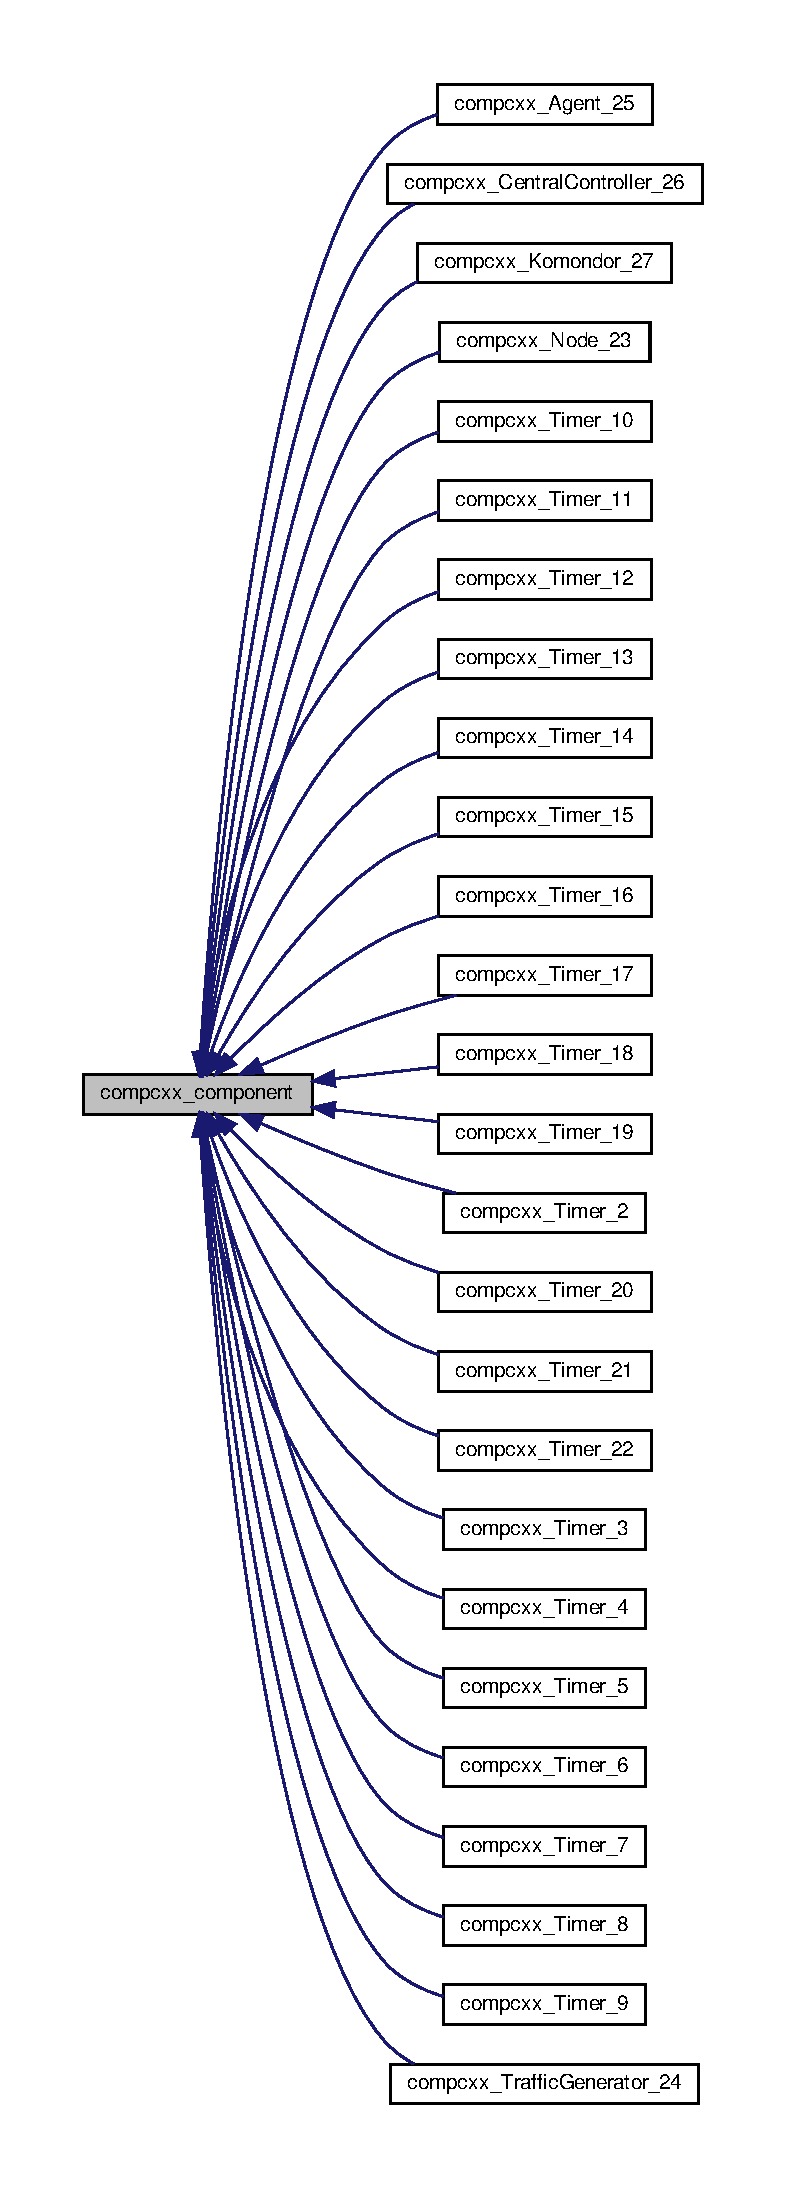
\includegraphics[height=550pt]{classcompcxx__component__inherit__graph}
\end{center}
\end{figure}
\subsection*{Public Types}
\begin{DoxyCompactItemize}
\item 
\mbox{\Hypertarget{classcompcxx__component_ae77339bcc9d37cfd73c7e86d83543c61}\label{classcompcxx__component_ae77339bcc9d37cfd73c7e86d83543c61}} 
typedef void(compcxx\+\_\+component\+::$\ast$ {\bfseries Agent\+\_\+outport\+Request\+Information\+To\+Ap\+\_\+f\+\_\+t}) ()
\item 
\mbox{\Hypertarget{classcompcxx__component_a2e6fd05abf2108270e0dc36fb77b8a2d}\label{classcompcxx__component_a2e6fd05abf2108270e0dc36fb77b8a2d}} 
typedef void(compcxx\+\_\+component\+::$\ast$ {\bfseries Agent\+\_\+outport\+Send\+Configuration\+To\+Ap\+\_\+f\+\_\+t}) (\hyperlink{structConfiguration}{Configuration} \&new\+\_\+configuration)
\item 
\mbox{\Hypertarget{classcompcxx__component_a8be04622edac273e160bc18b3c8ebadc}\label{classcompcxx__component_a8be04622edac273e160bc18b3c8ebadc}} 
typedef void(compcxx\+\_\+component\+::$\ast$ {\bfseries Agent\+\_\+outport\+Answer\+To\+Controller\+\_\+f\+\_\+t}) (\hyperlink{structConfiguration}{Configuration} \&configuration, \hyperlink{structPerformance}{Performance} \&performance, int agent\+\_\+id)
\item 
\mbox{\Hypertarget{classcompcxx__component_a96f2070a90e7f2b6b51ad972c5f58f38}\label{classcompcxx__component_a96f2070a90e7f2b6b51ad972c5f58f38}} 
typedef void(compcxx\+\_\+component\+::$\ast$ {\bfseries Central\+Controller\+\_\+outport\+Request\+Information\+To\+Agent\+\_\+f\+\_\+t}) (int destination\+\_\+agent\+\_\+id)
\item 
\mbox{\Hypertarget{classcompcxx__component_a7db4fd9662f71cf4ad302d6e9eec1efd}\label{classcompcxx__component_a7db4fd9662f71cf4ad302d6e9eec1efd}} 
typedef void(compcxx\+\_\+component\+::$\ast$ {\bfseries Central\+Controller\+\_\+outport\+Send\+Configuration\+To\+Agent\+\_\+f\+\_\+t}) (int destination\+\_\+agent\+\_\+id, \hyperlink{structConfiguration}{Configuration} \&new\+\_\+configuration, int controller\+\_\+mode)
\item 
\mbox{\Hypertarget{classcompcxx__component_a5bc681af4779c999f76e3cfa9bd446b1}\label{classcompcxx__component_a5bc681af4779c999f76e3cfa9bd446b1}} 
typedef void(compcxx\+\_\+component\+::$\ast$ {\bfseries Node\+\_\+outport\+Self\+Start\+T\+X\+\_\+f\+\_\+t}) (\hyperlink{structNotification}{Notification} \&notification)
\item 
\mbox{\Hypertarget{classcompcxx__component_a862b0c9aa0a29f8db0e7fa5c9d30f627}\label{classcompcxx__component_a862b0c9aa0a29f8db0e7fa5c9d30f627}} 
typedef void(compcxx\+\_\+component\+::$\ast$ {\bfseries Node\+\_\+outport\+Self\+Finish\+T\+X\+\_\+f\+\_\+t}) (\hyperlink{structNotification}{Notification} \&notification)
\item 
\mbox{\Hypertarget{classcompcxx__component_a089908d5367f9c1ae42739e55cf3b25a}\label{classcompcxx__component_a089908d5367f9c1ae42739e55cf3b25a}} 
typedef void(compcxx\+\_\+component\+::$\ast$ {\bfseries Node\+\_\+outport\+Send\+Logical\+Nack\+\_\+f\+\_\+t}) (\hyperlink{structLogicalNack}{Logical\+Nack} \&logical\+\_\+nack\+\_\+info)
\item 
\mbox{\Hypertarget{classcompcxx__component_aadb97834bcb0f5bc3b8cd79713f62944}\label{classcompcxx__component_aadb97834bcb0f5bc3b8cd79713f62944}} 
typedef void(compcxx\+\_\+component\+::$\ast$ {\bfseries Node\+\_\+outport\+Ask\+For\+Tx\+Modulation\+\_\+f\+\_\+t}) (\hyperlink{structNotification}{Notification} \&notification)
\item 
\mbox{\Hypertarget{classcompcxx__component_af69a02618a8d2f8f6c1c9792a92c459f}\label{classcompcxx__component_af69a02618a8d2f8f6c1c9792a92c459f}} 
typedef void(compcxx\+\_\+component\+::$\ast$ {\bfseries Node\+\_\+outport\+Answer\+Tx\+Modulation\+\_\+f\+\_\+t}) (\hyperlink{structNotification}{Notification} \&notification)
\item 
\mbox{\Hypertarget{classcompcxx__component_a0eb11913f26856b9ceb28385f299fa7e}\label{classcompcxx__component_a0eb11913f26856b9ceb28385f299fa7e}} 
typedef void(compcxx\+\_\+component\+::$\ast$ {\bfseries Node\+\_\+outport\+Answer\+To\+Agent\+\_\+f\+\_\+t}) (\hyperlink{structConfiguration}{Configuration} \&configuration, \hyperlink{structPerformance}{Performance} \&performance)
\item 
\mbox{\Hypertarget{classcompcxx__component_a0e928bd77e9c27615ff88f8b49f7b68b}\label{classcompcxx__component_a0e928bd77e9c27615ff88f8b49f7b68b}} 
typedef void(compcxx\+\_\+component\+::$\ast$ {\bfseries Node\+\_\+outport\+Set\+New\+Wlan\+Configuration\+\_\+f\+\_\+t}) (\hyperlink{structConfiguration}{Configuration} \&new\+\_\+configuration)
\item 
\mbox{\Hypertarget{classcompcxx__component_a1adf2972a45d9b9e3bc296cde6bebe98}\label{classcompcxx__component_a1adf2972a45d9b9e3bc296cde6bebe98}} 
typedef void(compcxx\+\_\+component\+::$\ast$ {\bfseries Node\+\_\+outport\+Request\+Spatial\+Reuse\+Configuration\+\_\+f\+\_\+t}) ()
\item 
\mbox{\Hypertarget{classcompcxx__component_a5f94013d79c964e4357a3b0fe6bc6b5e}\label{classcompcxx__component_a5f94013d79c964e4357a3b0fe6bc6b5e}} 
typedef void(compcxx\+\_\+component\+::$\ast$ {\bfseries Node\+\_\+outport\+New\+Spatial\+Reuse\+Configuration\+\_\+f\+\_\+t}) (\hyperlink{structConfiguration}{Configuration} \&new\+\_\+configuration)
\item 
\mbox{\Hypertarget{classcompcxx__component_a51b3469f64029d17b27e951265aa146b}\label{classcompcxx__component_a51b3469f64029d17b27e951265aa146b}} 
typedef void(compcxx\+\_\+component\+::$\ast$ {\bfseries Traffic\+Generator\+\_\+outport\+New\+Packet\+Generated\+\_\+f\+\_\+t}) ()
\end{DoxyCompactItemize}


The documentation for this class was generated from the following file\+:\begin{DoxyCompactItemize}
\item 
Code/main/compcxx\+\_\+komondor\+\_\+main.\+h\end{DoxyCompactItemize}

\hypertarget{classcompcxx__functor}{}\section{compcxx\+\_\+functor$<$ T $>$ Class Template Reference}
\label{classcompcxx__functor}\index{compcxx\+\_\+functor$<$ T $>$@{compcxx\+\_\+functor$<$ T $>$}}
\subsection*{Public Member Functions}
\begin{DoxyCompactItemize}
\item 
\mbox{\Hypertarget{classcompcxx__functor_a7b3e1bd13bee34e4cd1d6244fcff6031}\label{classcompcxx__functor_a7b3e1bd13bee34e4cd1d6244fcff6031}} 
void {\bfseries Connect} (\hyperlink{classcompcxx__component}{compcxx\+\_\+component} \&\+\_\+c, T \+\_\+f)
\end{DoxyCompactItemize}
\subsection*{Protected Attributes}
\begin{DoxyCompactItemize}
\item 
\mbox{\Hypertarget{classcompcxx__functor_ac716643013a9ff09b2fa7d36d3abf9a9}\label{classcompcxx__functor_ac716643013a9ff09b2fa7d36d3abf9a9}} 
std\+::vector$<$ \hyperlink{classcompcxx__component}{compcxx\+\_\+component} $\ast$ $>$ {\bfseries c}
\item 
\mbox{\Hypertarget{classcompcxx__functor_af5bb981608846fe8b4801a33238e98d3}\label{classcompcxx__functor_af5bb981608846fe8b4801a33238e98d3}} 
std\+::vector$<$ T $>$ {\bfseries f}
\end{DoxyCompactItemize}


The documentation for this class was generated from the following file\+:\begin{DoxyCompactItemize}
\item 
Code/main/compcxx\+\_\+komondor\+\_\+main.\+h\end{DoxyCompactItemize}

\hypertarget{classcompcxx__Komondor__27}{}\section{compcxx\+\_\+\+Komondor\+\_\+27 Class Reference}
\label{classcompcxx__Komondor__27}\index{compcxx\+\_\+\+Komondor\+\_\+27@{compcxx\+\_\+\+Komondor\+\_\+27}}


Inheritance diagram for compcxx\+\_\+\+Komondor\+\_\+27\+:\nopagebreak
\begin{figure}[H]
\begin{center}
\leavevmode
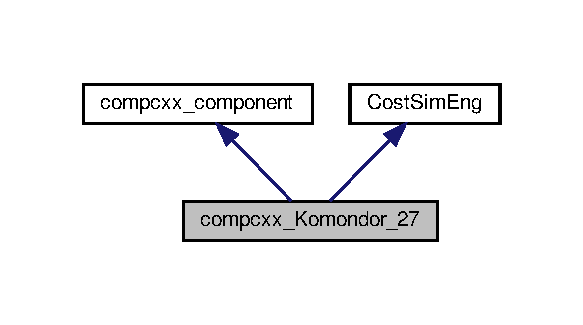
\includegraphics[width=280pt]{classcompcxx__Komondor__27__inherit__graph}
\end{center}
\end{figure}


Collaboration diagram for compcxx\+\_\+\+Komondor\+\_\+27\+:\nopagebreak
\begin{figure}[H]
\begin{center}
\leavevmode
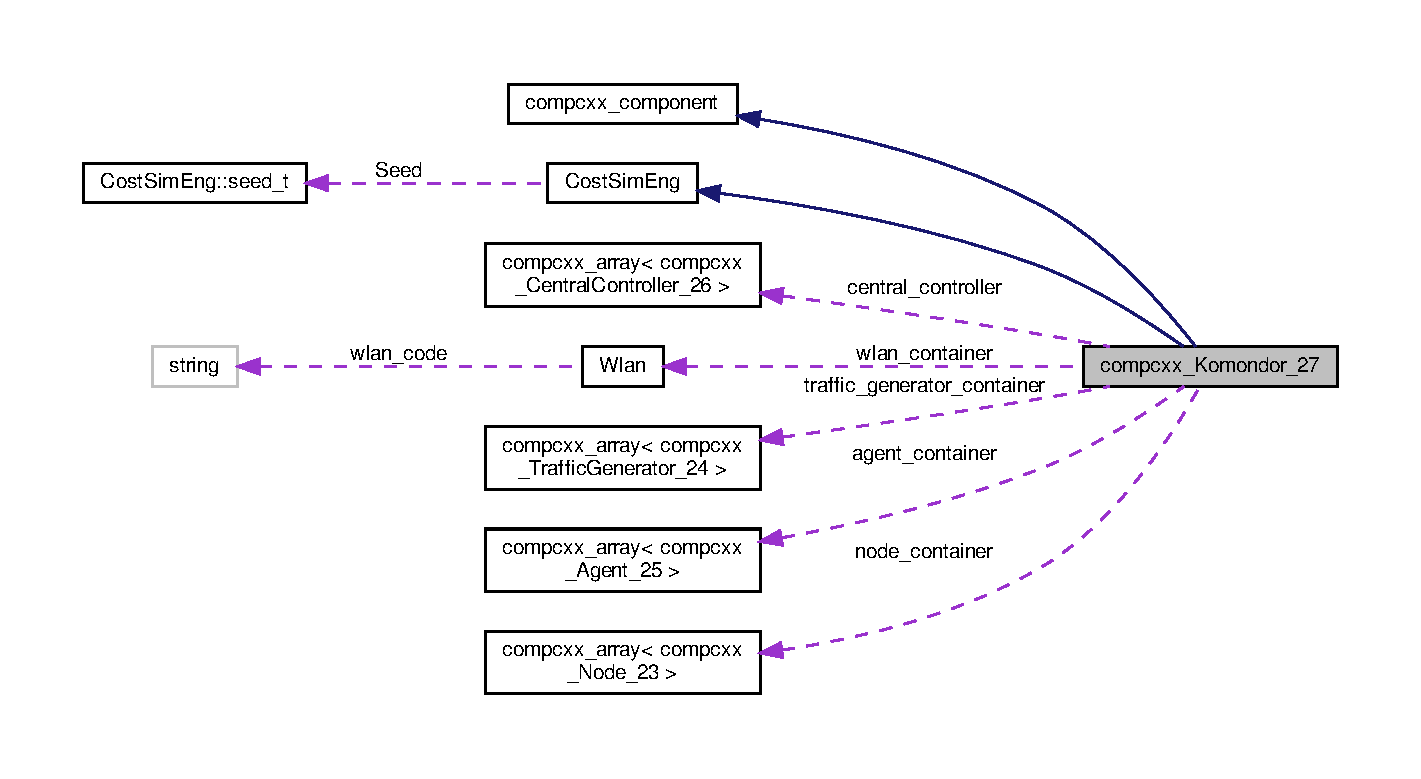
\includegraphics[width=350pt]{classcompcxx__Komondor__27__coll__graph}
\end{center}
\end{figure}
\subsection*{Public Member Functions}
\begin{DoxyCompactItemize}
\item 
\mbox{\Hypertarget{classcompcxx__Komondor__27_aae1cba60a8e176c95ec24d84f1e484ae}\label{classcompcxx__Komondor__27_aae1cba60a8e176c95ec24d84f1e484ae}} 
void {\bfseries Setup} (double simulation\+\_\+time\+\_\+komondor, int save\+\_\+system\+\_\+logs, int save\+\_\+node\+\_\+logs, int save\+\_\+agent\+\_\+logs, int print\+\_\+node\+\_\+logs, int print\+\_\+system\+\_\+logs, int print\+\_\+agent\+\_\+logs, const char $\ast$system\+\_\+filename, const char $\ast$nodes\+\_\+filename, const char $\ast$script\+\_\+filename, const char $\ast$simulation\+\_\+code, int seed\+\_\+console, int agents\+\_\+enabled, const char $\ast$agents\+\_\+filename)
\item 
\mbox{\Hypertarget{classcompcxx__Komondor__27_a74a60c428bf2dce5a0cec25d7341c5fd}\label{classcompcxx__Komondor__27_a74a60c428bf2dce5a0cec25d7341c5fd}} 
void {\bfseries Stop} ()
\item 
\mbox{\Hypertarget{classcompcxx__Komondor__27_ad6ca963a42e5beff600747d1249b9360}\label{classcompcxx__Komondor__27_ad6ca963a42e5beff600747d1249b9360}} 
void {\bfseries Start} ()
\item 
\mbox{\Hypertarget{classcompcxx__Komondor__27_a6735e289f86ba3288607281f4d8e8cd0}\label{classcompcxx__Komondor__27_a6735e289f86ba3288607281f4d8e8cd0}} 
void {\bfseries Input\+Checker} ()
\item 
\mbox{\Hypertarget{classcompcxx__Komondor__27_a9158afcdccfefdebebc4e25920e28c78}\label{classcompcxx__Komondor__27_a9158afcdccfefdebebc4e25920e28c78}} 
void {\bfseries Setup\+Environment\+By\+Reading\+Input\+File} (const char $\ast$system\+\_\+filename)
\item 
\mbox{\Hypertarget{classcompcxx__Komondor__27_a85df144f45a28b3abc84ed45447913fb}\label{classcompcxx__Komondor__27_a85df144f45a28b3abc84ed45447913fb}} 
void {\bfseries Generate\+Nodes\+By\+Reading\+Input\+File} (const char $\ast$nodes\+\_\+filename)
\item 
\mbox{\Hypertarget{classcompcxx__Komondor__27_a9886605add430e49e119ad5a91438151}\label{classcompcxx__Komondor__27_a9886605add430e49e119ad5a91438151}} 
void {\bfseries Generate\+Agents} (const char $\ast$agents\+\_\+filename)
\item 
\mbox{\Hypertarget{classcompcxx__Komondor__27_a2c99bfcd07b40a577c136e5396e9ac4a}\label{classcompcxx__Komondor__27_a2c99bfcd07b40a577c136e5396e9ac4a}} 
void {\bfseries Generate\+Central\+Controller} (const char $\ast$agents\+\_\+filename)
\item 
\mbox{\Hypertarget{classcompcxx__Komondor__27_aab5cb7d69218b4c26ba1635abbc1c10d}\label{classcompcxx__Komondor__27_aab5cb7d69218b4c26ba1635abbc1c10d}} 
int {\bfseries Get\+Num\+Of\+Lines} (const char $\ast$nodes\+\_\+filename)
\item 
\mbox{\Hypertarget{classcompcxx__Komondor__27_a6e1d577a7bbc4995ebcf8dc0e9dc55e3}\label{classcompcxx__Komondor__27_a6e1d577a7bbc4995ebcf8dc0e9dc55e3}} 
int {\bfseries Get\+Num\+Of\+Nodes} (const char $\ast$nodes\+\_\+filename, int node\+\_\+type, std\+::string wlan\+\_\+code)
\item 
\mbox{\Hypertarget{classcompcxx__Komondor__27_aa9440e8685f2f2df0cfe2e15833e6817}\label{classcompcxx__Komondor__27_aa9440e8685f2f2df0cfe2e15833e6817}} 
void {\bfseries Print\+System\+Info} ()
\item 
\mbox{\Hypertarget{classcompcxx__Komondor__27_ab3913b053b3c0d726c56a12e51e57585}\label{classcompcxx__Komondor__27_ab3913b053b3c0d726c56a12e51e57585}} 
void {\bfseries Print\+All\+Wlans\+Info} ()
\item 
\mbox{\Hypertarget{classcompcxx__Komondor__27_a58807e58cc62af62f66b16dbcf4bb29f}\label{classcompcxx__Komondor__27_a58807e58cc62af62f66b16dbcf4bb29f}} 
void {\bfseries Print\+All\+Agents\+Info} ()
\item 
\mbox{\Hypertarget{classcompcxx__Komondor__27_ab8335a20831b55ac1f1a9b10ff2767a6}\label{classcompcxx__Komondor__27_ab8335a20831b55ac1f1a9b10ff2767a6}} 
void {\bfseries Print\+Central\+Controller\+Info} ()
\item 
\mbox{\Hypertarget{classcompcxx__Komondor__27_aa276649f84ccf1f260a0b1b2eaee65f0}\label{classcompcxx__Komondor__27_aa276649f84ccf1f260a0b1b2eaee65f0}} 
void {\bfseries Print\+All\+Nodes\+Info} (int info\+\_\+detail\+\_\+level)
\item 
\mbox{\Hypertarget{classcompcxx__Komondor__27_a4f7651e20f499842bb4dbaaebc8878b9}\label{classcompcxx__Komondor__27_a4f7651e20f499842bb4dbaaebc8878b9}} 
void {\bfseries Print\+Ml\+Operation\+Info} ()
\item 
\mbox{\Hypertarget{classcompcxx__Komondor__27_a14875aea46ab2caa660dea3b760e5f41}\label{classcompcxx__Komondor__27_a14875aea46ab2caa660dea3b760e5f41}} 
void {\bfseries Write\+System\+Info} (\hyperlink{structLogger}{Logger} logger)
\item 
\mbox{\Hypertarget{classcompcxx__Komondor__27_a7a55b574d7e52e764d01b37cf880015e}\label{classcompcxx__Komondor__27_a7a55b574d7e52e764d01b37cf880015e}} 
void {\bfseries Write\+All\+Wlans\+Info} (\hyperlink{structLogger}{Logger} logger, std\+::string header\+\_\+str)
\item 
\mbox{\Hypertarget{classcompcxx__Komondor__27_a36591aff6be24f546405c5f5b98c3762}\label{classcompcxx__Komondor__27_a36591aff6be24f546405c5f5b98c3762}} 
void {\bfseries Write\+All\+Nodes\+Info} (\hyperlink{structLogger}{Logger} logger, int info\+\_\+detail\+\_\+level, std\+::string header\+\_\+str)
\item 
\mbox{\Hypertarget{classcompcxx__Komondor__27_a693426c10b883f79d295980b9de2d160}\label{classcompcxx__Komondor__27_a693426c10b883f79d295980b9de2d160}} 
void {\bfseries Write\+All\+Agents\+Info} (\hyperlink{structLogger}{Logger} logger, std\+::string header\+\_\+str)
\item 
\mbox{\Hypertarget{classcompcxx__Komondor__27_ac523ba46f25c317b3931fde7dfd5f0fa}\label{classcompcxx__Komondor__27_ac523ba46f25c317b3931fde7dfd5f0fa}} 
void {\bfseries Read\+System\+Configuration\+File} ()
\end{DoxyCompactItemize}
\subsection*{Public Attributes}
\begin{DoxyCompactItemize}
\item 
\mbox{\Hypertarget{classcompcxx__Komondor__27_a692da1796d5382c731ffd5409efa568f}\label{classcompcxx__Komondor__27_a692da1796d5382c731ffd5409efa568f}} 
\hyperlink{classcompcxx__array}{compcxx\+\_\+array}$<$ \hyperlink{classcompcxx__Node__23}{compcxx\+\_\+\+Node\+\_\+23} $>$ {\bfseries node\+\_\+container}
\item 
\mbox{\Hypertarget{classcompcxx__Komondor__27_a3d2dabf215a7d2507a027b68a368aca6}\label{classcompcxx__Komondor__27_a3d2dabf215a7d2507a027b68a368aca6}} 
\hyperlink{structWlan}{Wlan} $\ast$ {\bfseries wlan\+\_\+container}
\item 
\mbox{\Hypertarget{classcompcxx__Komondor__27_ad10bf64db052746ed6722bc10d39f67b}\label{classcompcxx__Komondor__27_ad10bf64db052746ed6722bc10d39f67b}} 
\hyperlink{classcompcxx__array}{compcxx\+\_\+array}$<$ \hyperlink{classcompcxx__TrafficGenerator__24}{compcxx\+\_\+\+Traffic\+Generator\+\_\+24} $>$ {\bfseries traffic\+\_\+generator\+\_\+container}
\item 
\mbox{\Hypertarget{classcompcxx__Komondor__27_affd3dde760ede4b09250ba72b9ce55d1}\label{classcompcxx__Komondor__27_affd3dde760ede4b09250ba72b9ce55d1}} 
int {\bfseries total\+\_\+wlans\+\_\+number}
\item 
\mbox{\Hypertarget{classcompcxx__Komondor__27_a02563f280ffb977aba7a7fa7bdb35a7f}\label{classcompcxx__Komondor__27_a02563f280ffb977aba7a7fa7bdb35a7f}} 
int {\bfseries total\+\_\+agents\+\_\+number}
\item 
\mbox{\Hypertarget{classcompcxx__Komondor__27_aa1a8144a72ea5bc1c03e460817cb2dc2}\label{classcompcxx__Komondor__27_aa1a8144a72ea5bc1c03e460817cb2dc2}} 
int {\bfseries total\+\_\+controlled\+\_\+agents\+\_\+number} = 0
\item 
\mbox{\Hypertarget{classcompcxx__Komondor__27_a244efdc09681b32a68281bf518ecf96f}\label{classcompcxx__Komondor__27_a244efdc09681b32a68281bf518ecf96f}} 
int {\bfseries save\+\_\+node\+\_\+logs}
\item 
\mbox{\Hypertarget{classcompcxx__Komondor__27_aa541b81abcef052371ac1b51a089868d}\label{classcompcxx__Komondor__27_aa541b81abcef052371ac1b51a089868d}} 
int {\bfseries print\+\_\+node\+\_\+logs}
\item 
\mbox{\Hypertarget{classcompcxx__Komondor__27_a7437c9f3c822ef29adeed7b7a36d4180}\label{classcompcxx__Komondor__27_a7437c9f3c822ef29adeed7b7a36d4180}} 
int {\bfseries save\+\_\+agent\+\_\+logs}
\item 
\mbox{\Hypertarget{classcompcxx__Komondor__27_a678de1e71bbf9b8d04e95f7b3d086066}\label{classcompcxx__Komondor__27_a678de1e71bbf9b8d04e95f7b3d086066}} 
int {\bfseries print\+\_\+agent\+\_\+logs}
\item 
\mbox{\Hypertarget{classcompcxx__Komondor__27_a1a318fb2cb2ba5b27503336fa54c3a46}\label{classcompcxx__Komondor__27_a1a318fb2cb2ba5b27503336fa54c3a46}} 
double {\bfseries simulation\+\_\+time\+\_\+komondor}
\item 
\mbox{\Hypertarget{classcompcxx__Komondor__27_a376c38447ffeb9dd746435af4811dd7b}\label{classcompcxx__Komondor__27_a376c38447ffeb9dd746435af4811dd7b}} 
int {\bfseries num\+\_\+channels\+\_\+komondor}
\item 
\mbox{\Hypertarget{classcompcxx__Komondor__27_aaa1cdffb6b7fe47c7f01d747ae8675e5}\label{classcompcxx__Komondor__27_aaa1cdffb6b7fe47c7f01d747ae8675e5}} 
double {\bfseries basic\+\_\+channel\+\_\+bandwidth}
\item 
\mbox{\Hypertarget{classcompcxx__Komondor__27_a5b65ead9def34b61954603f492afdf61}\label{classcompcxx__Komondor__27_a5b65ead9def34b61954603f492afdf61}} 
int {\bfseries pdf\+\_\+backoff}
\item 
\mbox{\Hypertarget{classcompcxx__Komondor__27_ac05e5f7cb6d8a4cc3fde1e4a3233df14}\label{classcompcxx__Komondor__27_ac05e5f7cb6d8a4cc3fde1e4a3233df14}} 
int {\bfseries pdf\+\_\+tx\+\_\+time}
\item 
\mbox{\Hypertarget{classcompcxx__Komondor__27_a6b1f0ced58a6165527edbae400e83740}\label{classcompcxx__Komondor__27_a6b1f0ced58a6165527edbae400e83740}} 
int {\bfseries frame\+\_\+length}
\item 
\mbox{\Hypertarget{classcompcxx__Komondor__27_a16168a77b38cb5949c03fd829ebff152}\label{classcompcxx__Komondor__27_a16168a77b38cb5949c03fd829ebff152}} 
int {\bfseries ack\+\_\+length}
\item 
\mbox{\Hypertarget{classcompcxx__Komondor__27_abc3c181293dcf89425d85a9578dbbc4f}\label{classcompcxx__Komondor__27_abc3c181293dcf89425d85a9578dbbc4f}} 
int {\bfseries rts\+\_\+length}
\item 
\mbox{\Hypertarget{classcompcxx__Komondor__27_a9a634e01855e720663f0874f05d1fbe1}\label{classcompcxx__Komondor__27_a9a634e01855e720663f0874f05d1fbe1}} 
int {\bfseries cts\+\_\+length}
\item 
\mbox{\Hypertarget{classcompcxx__Komondor__27_a43e7c5457d161a58559c4ec0f4ac5771}\label{classcompcxx__Komondor__27_a43e7c5457d161a58559c4ec0f4ac5771}} 
int {\bfseries max\+\_\+num\+\_\+packets\+\_\+aggregated}
\item 
\mbox{\Hypertarget{classcompcxx__Komondor__27_ae59d4cb32b46724f000f9fe8d39a1f75}\label{classcompcxx__Komondor__27_ae59d4cb32b46724f000f9fe8d39a1f75}} 
int {\bfseries path\+\_\+loss\+\_\+model}
\item 
\mbox{\Hypertarget{classcompcxx__Komondor__27_ad0fede65539fe8930c43bb06b07e1f16}\label{classcompcxx__Komondor__27_ad0fede65539fe8930c43bb06b07e1f16}} 
double {\bfseries capture\+\_\+effect}
\item 
\mbox{\Hypertarget{classcompcxx__Komondor__27_a8dfa55183c60c6c3397f8d5e4d7ee805}\label{classcompcxx__Komondor__27_a8dfa55183c60c6c3397f8d5e4d7ee805}} 
double {\bfseries noise\+\_\+level}
\item 
\mbox{\Hypertarget{classcompcxx__Komondor__27_afa65ff1e8fc27c32fe2d0418ccf12e65}\label{classcompcxx__Komondor__27_afa65ff1e8fc27c32fe2d0418ccf12e65}} 
int {\bfseries adjacent\+\_\+channel\+\_\+model}
\item 
\mbox{\Hypertarget{classcompcxx__Komondor__27_a6250026dc1301f185cb37e3f8d6d49f2}\label{classcompcxx__Komondor__27_a6250026dc1301f185cb37e3f8d6d49f2}} 
int {\bfseries collisions\+\_\+model}
\item 
\mbox{\Hypertarget{classcompcxx__Komondor__27_a59c89284ba027d8131845762b09d62ed}\label{classcompcxx__Komondor__27_a59c89284ba027d8131845762b09d62ed}} 
double {\bfseries constant\+\_\+per}
\item 
\mbox{\Hypertarget{classcompcxx__Komondor__27_a7b7d1c435f9e857795fcd78b83235367}\label{classcompcxx__Komondor__27_a7b7d1c435f9e857795fcd78b83235367}} 
int {\bfseries traffic\+\_\+model}
\item 
\mbox{\Hypertarget{classcompcxx__Komondor__27_a270c2a2667913924cd09f6ef1c190cd6}\label{classcompcxx__Komondor__27_a270c2a2667913924cd09f6ef1c190cd6}} 
int {\bfseries backoff\+\_\+type}
\item 
\mbox{\Hypertarget{classcompcxx__Komondor__27_aacc15e3c04280a509e5b195d03468e16}\label{classcompcxx__Komondor__27_aacc15e3c04280a509e5b195d03468e16}} 
int {\bfseries cw\+\_\+adaptation}
\item 
\mbox{\Hypertarget{classcompcxx__Komondor__27_a4833d05fd70e6d0cc7a4130eea5785e6}\label{classcompcxx__Komondor__27_a4833d05fd70e6d0cc7a4130eea5785e6}} 
int {\bfseries pifs\+\_\+activated}
\item 
\mbox{\Hypertarget{classcompcxx__Komondor__27_a2608c3f89995ee0cf662a2b81ed9557e}\label{classcompcxx__Komondor__27_a2608c3f89995ee0cf662a2b81ed9557e}} 
int {\bfseries capture\+\_\+effect\+\_\+model}
\item 
\mbox{\Hypertarget{classcompcxx__Komondor__27_ad8c341fe2e5f1752fbbb8a4d0d82315b}\label{classcompcxx__Komondor__27_ad8c341fe2e5f1752fbbb8a4d0d82315b}} 
int {\bfseries agents\+\_\+enabled}
\item 
\mbox{\Hypertarget{classcompcxx__Komondor__27_a0c84a07ddb506e8fcf39b3df53694e48}\label{classcompcxx__Komondor__27_a0c84a07ddb506e8fcf39b3df53694e48}} 
\hyperlink{classcompcxx__array}{compcxx\+\_\+array}$<$ \hyperlink{classcompcxx__Agent__25}{compcxx\+\_\+\+Agent\+\_\+25} $>$ {\bfseries agent\+\_\+container}
\item 
\mbox{\Hypertarget{classcompcxx__Komondor__27_a3dd07c6012e9d97f9c8c7b378d658a11}\label{classcompcxx__Komondor__27_a3dd07c6012e9d97f9c8c7b378d658a11}} 
int {\bfseries num\+\_\+actions\+\_\+channel}
\item 
\mbox{\Hypertarget{classcompcxx__Komondor__27_ae7e343e99ce6848638e4af5b5f22887a}\label{classcompcxx__Komondor__27_ae7e343e99ce6848638e4af5b5f22887a}} 
int {\bfseries num\+\_\+actions\+\_\+sensitivity}
\item 
\mbox{\Hypertarget{classcompcxx__Komondor__27_a0586fc1ed648eb37b1ddbcceb7a7fe8a}\label{classcompcxx__Komondor__27_a0586fc1ed648eb37b1ddbcceb7a7fe8a}} 
int {\bfseries num\+\_\+actions\+\_\+tx\+\_\+power}
\item 
\mbox{\Hypertarget{classcompcxx__Komondor__27_a8470be07bb5bf607fa0d28131cf2fcb5}\label{classcompcxx__Komondor__27_a8470be07bb5bf607fa0d28131cf2fcb5}} 
int {\bfseries num\+\_\+actions\+\_\+dcb\+\_\+policy}
\item 
\mbox{\Hypertarget{classcompcxx__Komondor__27_adb8e5f0a4d6e1d6dff05e09f945a9eb9}\label{classcompcxx__Komondor__27_adb8e5f0a4d6e1d6dff05e09f945a9eb9}} 
double $\ast$ {\bfseries actions\+\_\+pd}
\item 
\mbox{\Hypertarget{classcompcxx__Komondor__27_a65c79608c259c00aad2391d9510ca369}\label{classcompcxx__Komondor__27_a65c79608c259c00aad2391d9510ca369}} 
double $\ast$ {\bfseries actions\+\_\+tx\+\_\+power}
\item 
\mbox{\Hypertarget{classcompcxx__Komondor__27_a952a605a9fc1418b6993abbdf297e2b5}\label{classcompcxx__Komondor__27_a952a605a9fc1418b6993abbdf297e2b5}} 
\hyperlink{classcompcxx__array}{compcxx\+\_\+array}$<$ \hyperlink{classcompcxx__CentralController__26}{compcxx\+\_\+\+Central\+Controller\+\_\+26} $>$ {\bfseries central\+\_\+controller}
\end{DoxyCompactItemize}
\subsection*{Additional Inherited Members}


The documentation for this class was generated from the following file\+:\begin{DoxyCompactItemize}
\item 
Code/main/komondor\+\_\+main.\+cxx\end{DoxyCompactItemize}

\hypertarget{classcompcxx__Node__23}{}\section{compcxx\+\_\+\+Node\+\_\+23 Class Reference}
\label{classcompcxx__Node__23}\index{compcxx\+\_\+\+Node\+\_\+23@{compcxx\+\_\+\+Node\+\_\+23}}


Inheritance diagram for compcxx\+\_\+\+Node\+\_\+23\+:\nopagebreak
\begin{figure}[H]
\begin{center}
\leavevmode
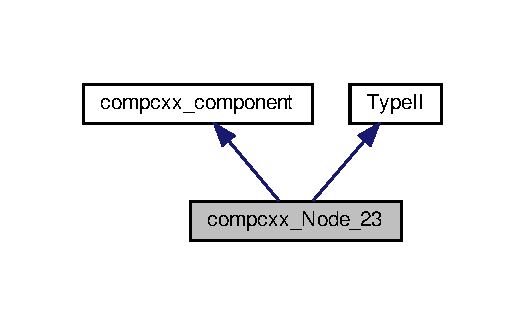
\includegraphics[width=252pt]{classcompcxx__Node__23__inherit__graph}
\end{center}
\end{figure}


Collaboration diagram for compcxx\+\_\+\+Node\+\_\+23\+:\nopagebreak
\begin{figure}[H]
\begin{center}
\leavevmode
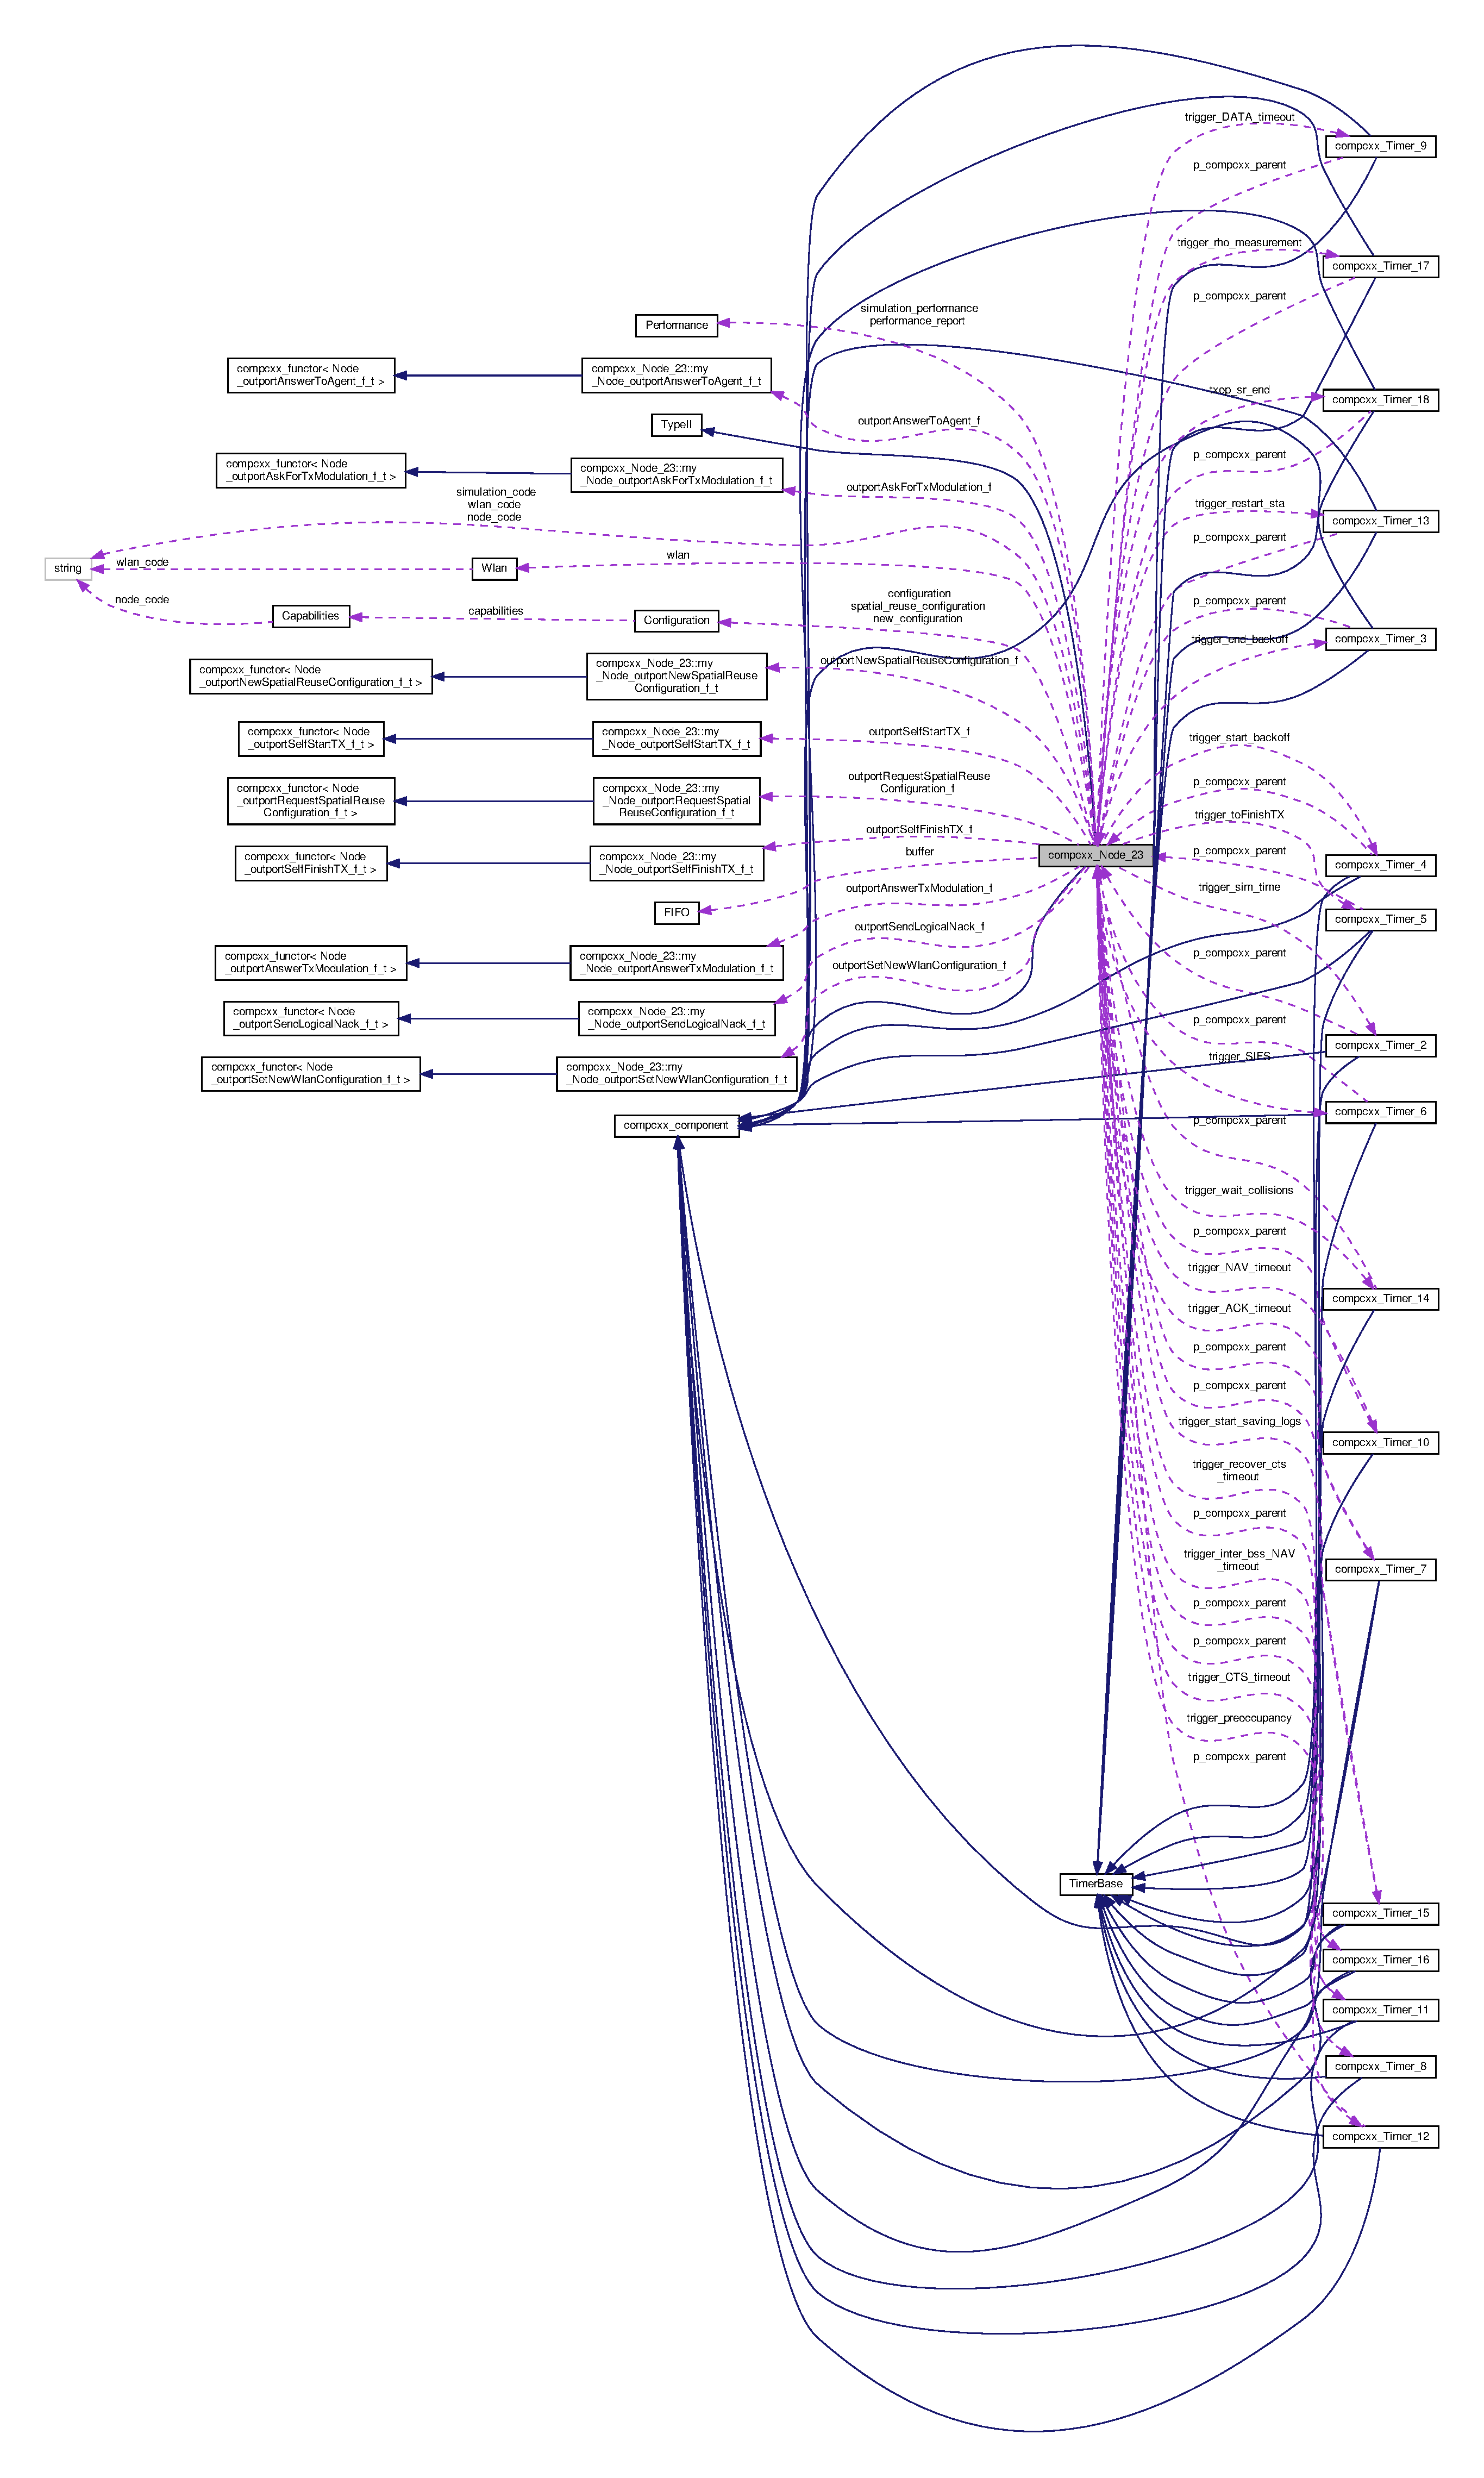
\includegraphics[height=550pt]{classcompcxx__Node__23__coll__graph}
\end{center}
\end{figure}
\subsection*{Classes}
\begin{DoxyCompactItemize}
\item 
class \hyperlink{classcompcxx__Node__23_1_1my__Node__outportAnswerToAgent__f__t}{my\+\_\+\+Node\+\_\+outport\+Answer\+To\+Agent\+\_\+f\+\_\+t}
\item 
class \hyperlink{classcompcxx__Node__23_1_1my__Node__outportAnswerTxModulation__f__t}{my\+\_\+\+Node\+\_\+outport\+Answer\+Tx\+Modulation\+\_\+f\+\_\+t}
\item 
class \hyperlink{classcompcxx__Node__23_1_1my__Node__outportAskForTxModulation__f__t}{my\+\_\+\+Node\+\_\+outport\+Ask\+For\+Tx\+Modulation\+\_\+f\+\_\+t}
\item 
class \hyperlink{classcompcxx__Node__23_1_1my__Node__outportNewSpatialReuseConfiguration__f__t}{my\+\_\+\+Node\+\_\+outport\+New\+Spatial\+Reuse\+Configuration\+\_\+f\+\_\+t}
\item 
class \hyperlink{classcompcxx__Node__23_1_1my__Node__outportRequestSpatialReuseConfiguration__f__t}{my\+\_\+\+Node\+\_\+outport\+Request\+Spatial\+Reuse\+Configuration\+\_\+f\+\_\+t}
\item 
class \hyperlink{classcompcxx__Node__23_1_1my__Node__outportSelfFinishTX__f__t}{my\+\_\+\+Node\+\_\+outport\+Self\+Finish\+T\+X\+\_\+f\+\_\+t}
\item 
class \hyperlink{classcompcxx__Node__23_1_1my__Node__outportSelfStartTX__f__t}{my\+\_\+\+Node\+\_\+outport\+Self\+Start\+T\+X\+\_\+f\+\_\+t}
\item 
class \hyperlink{classcompcxx__Node__23_1_1my__Node__outportSendLogicalNack__f__t}{my\+\_\+\+Node\+\_\+outport\+Send\+Logical\+Nack\+\_\+f\+\_\+t}
\item 
class \hyperlink{classcompcxx__Node__23_1_1my__Node__outportSetNewWlanConfiguration__f__t}{my\+\_\+\+Node\+\_\+outport\+Set\+New\+Wlan\+Configuration\+\_\+f\+\_\+t}
\end{DoxyCompactItemize}
\subsection*{Public Member Functions}
\begin{DoxyCompactItemize}
\item 
\mbox{\Hypertarget{classcompcxx__Node__23_aa39779f39e893c00757ffdef42078693}\label{classcompcxx__Node__23_aa39779f39e893c00757ffdef42078693}} 
void {\bfseries Setup} ()
\item 
\mbox{\Hypertarget{classcompcxx__Node__23_ad14267bb799b7b4b2a107f5627ffb434}\label{classcompcxx__Node__23_ad14267bb799b7b4b2a107f5627ffb434}} 
void {\bfseries Start} ()
\item 
\mbox{\Hypertarget{classcompcxx__Node__23_a930a5e759b3e75800755fea2ab79bcc5}\label{classcompcxx__Node__23_a930a5e759b3e75800755fea2ab79bcc5}} 
void {\bfseries Stop} ()
\item 
\mbox{\Hypertarget{classcompcxx__Node__23_a787413f836a704ca5fc4af8544ecf8bb}\label{classcompcxx__Node__23_a787413f836a704ca5fc4af8544ecf8bb}} 
void {\bfseries Initialize\+Variables} ()
\item 
\mbox{\Hypertarget{classcompcxx__Node__23_aa1ce61c7c2df3faf489ad7d0ff91d3c4}\label{classcompcxx__Node__23_aa1ce61c7c2df3faf489ad7d0ff91d3c4}} 
void {\bfseries Restart\+Node} (int called\+\_\+by\+\_\+time\+\_\+out)
\item 
\mbox{\Hypertarget{classcompcxx__Node__23_ad17648e23643eb4ee70a9875abb9eebd}\label{classcompcxx__Node__23_ad17648e23643eb4ee70a9875abb9eebd}} 
void {\bfseries Call\+Restart\+Sta} ()
\item 
\mbox{\Hypertarget{classcompcxx__Node__23_a8a93628af7ac0059d7769dcbea892021}\label{classcompcxx__Node__23_a8a93628af7ac0059d7769dcbea892021}} 
void {\bfseries Call\+Sensing} ()
\item 
\mbox{\Hypertarget{classcompcxx__Node__23_a7989ab0105396bdc356e44ab8ed5b170}\label{classcompcxx__Node__23_a7989ab0105396bdc356e44ab8ed5b170}} 
void {\bfseries Print\+Node\+Info} (int info\+\_\+detail\+\_\+level)
\item 
\mbox{\Hypertarget{classcompcxx__Node__23_a1fb31d9f2ed4055a4068580af2287b44}\label{classcompcxx__Node__23_a1fb31d9f2ed4055a4068580af2287b44}} 
void {\bfseries Print\+Node\+Configuration} ()
\item 
\mbox{\Hypertarget{classcompcxx__Node__23_af73dc83c66e53a1a4e73ed31a5568807}\label{classcompcxx__Node__23_af73dc83c66e53a1a4e73ed31a5568807}} 
void {\bfseries Write\+Node\+Info} (\hyperlink{structLogger}{Logger} node\+\_\+logger, int info\+\_\+detail\+\_\+level, std\+::string header\+\_\+str)
\item 
\mbox{\Hypertarget{classcompcxx__Node__23_ac3ed406b3902c26fe1751b8044a42adf}\label{classcompcxx__Node__23_ac3ed406b3902c26fe1751b8044a42adf}} 
void {\bfseries Write\+Node\+Configuration} (\hyperlink{structLogger}{Logger} node\+\_\+logger, std\+::string header\+\_\+str)
\item 
\mbox{\Hypertarget{classcompcxx__Node__23_add479becdbcd125217992c3a3908cada}\label{classcompcxx__Node__23_add479becdbcd125217992c3a3908cada}} 
void {\bfseries Write\+Received\+Configuration} (\hyperlink{structLogger}{Logger} node\+\_\+logger, std\+::string header\+\_\+str, \hyperlink{structConfiguration}{Configuration} new\+\_\+configuration)
\item 
\mbox{\Hypertarget{classcompcxx__Node__23_adc029cc954973f04763ce6f522bbb784}\label{classcompcxx__Node__23_adc029cc954973f04763ce6f522bbb784}} 
void {\bfseries Print\+Or\+Write\+Node\+Statistics} (int write\+\_\+or\+\_\+print)
\item 
\mbox{\Hypertarget{classcompcxx__Node__23_a9631f9e8414c394b91f02e99e0d941f5}\label{classcompcxx__Node__23_a9631f9e8414c394b91f02e99e0d941f5}} 
void {\bfseries Handle\+Slotted\+Backoff\+Collision} ()
\item 
\mbox{\Hypertarget{classcompcxx__Node__23_a4b525bd45b73738b6b4e068f1fa50f3f}\label{classcompcxx__Node__23_a4b525bd45b73738b6b4e068f1fa50f3f}} 
void {\bfseries Start\+Saving\+Logs} ()
\item 
\mbox{\Hypertarget{classcompcxx__Node__23_a4cc2834c0231ad207c46d9f40949e3ba}\label{classcompcxx__Node__23_a4cc2834c0231ad207c46d9f40949e3ba}} 
void {\bfseries Recover\+From\+Cts\+Timeout} ()
\item 
\mbox{\Hypertarget{classcompcxx__Node__23_a3b763b74688ecd5341e5a34447d9791f}\label{classcompcxx__Node__23_a3b763b74688ecd5341e5a34447d9791f}} 
void {\bfseries Measure\+Rho} ()
\item 
\mbox{\Hypertarget{classcompcxx__Node__23_a4624de378d320dade9595f1951cfa54d}\label{classcompcxx__Node__23_a4624de378d320dade9595f1951cfa54d}} 
void {\bfseries Save\+Simulation\+Performance} ()
\item 
\mbox{\Hypertarget{classcompcxx__Node__23_aaaae36228f84db854724b930584c1fcf}\label{classcompcxx__Node__23_aaaae36228f84db854724b930584c1fcf}} 
\hyperlink{structNotification}{Notification} {\bfseries Generate\+Notification} (int packet\+\_\+type, int destination\+\_\+id, int packet\+\_\+id, int num\+\_\+packets\+\_\+aggregated, double timestamp\+\_\+generated, double tx\+\_\+duration)
\item 
\mbox{\Hypertarget{classcompcxx__Node__23_a6e0f6db0d765f141adaf2eaf226a513e}\label{classcompcxx__Node__23_a6e0f6db0d765f141adaf2eaf226a513e}} 
void {\bfseries Select\+Destination} ()
\item 
\mbox{\Hypertarget{classcompcxx__Node__23_a1dee89b6eb5a511d15f842d41f09a8d2}\label{classcompcxx__Node__23_a1dee89b6eb5a511d15f842d41f09a8d2}} 
void {\bfseries Send\+Response\+Packet} ()
\item 
\mbox{\Hypertarget{classcompcxx__Node__23_a34bf60a62ce77350e9efac3516a766ca}\label{classcompcxx__Node__23_a34bf60a62ce77350e9efac3516a766ca}} 
void {\bfseries Ack\+Timeout} ()
\item 
\mbox{\Hypertarget{classcompcxx__Node__23_a84999e7da3b655131d257d204cb5502f}\label{classcompcxx__Node__23_a84999e7da3b655131d257d204cb5502f}} 
void {\bfseries Cts\+Timeout} ()
\item 
\mbox{\Hypertarget{classcompcxx__Node__23_a90dfca805d82191d7e9d7017c289c46f}\label{classcompcxx__Node__23_a90dfca805d82191d7e9d7017c289c46f}} 
void {\bfseries Data\+Timeout} ()
\item 
\mbox{\Hypertarget{classcompcxx__Node__23_a35905e848f7592b9d2dfe98349b43bc0}\label{classcompcxx__Node__23_a35905e848f7592b9d2dfe98349b43bc0}} 
void {\bfseries Nav\+Timeout} ()
\item 
\mbox{\Hypertarget{classcompcxx__Node__23_aaff7be853e3904fff1211d5dab6bb1b0}\label{classcompcxx__Node__23_aaff7be853e3904fff1211d5dab6bb1b0}} 
void {\bfseries Request\+M\+CS} ()
\item 
\mbox{\Hypertarget{classcompcxx__Node__23_a30702ef96e7643cc943fbbf01ac4b8d0}\label{classcompcxx__Node__23_a30702ef96e7643cc943fbbf01ac4b8d0}} 
void {\bfseries Start\+Transmission} ()
\item 
\mbox{\Hypertarget{classcompcxx__Node__23_a1707011836a1260ed7f266b1c54a7e14}\label{classcompcxx__Node__23_a1707011836a1260ed7f266b1c54a7e14}} 
void {\bfseries Abort\+Rts\+Transmission} ()
\item 
\mbox{\Hypertarget{classcompcxx__Node__23_a1a57d975d6410b420bff7ddb91eee90e}\label{classcompcxx__Node__23_a1a57d975d6410b420bff7ddb91eee90e}} 
void {\bfseries Send\+Logical\+Nack} (\hyperlink{structLogicalNack}{Logical\+Nack} logical\+\_\+nack)
\item 
\mbox{\Hypertarget{classcompcxx__Node__23_a0e502bf77e44dff1f8c6d4c6f993269c}\label{classcompcxx__Node__23_a0e502bf77e44dff1f8c6d4c6f993269c}} 
void {\bfseries Pause\+Backoff} ()
\item 
\mbox{\Hypertarget{classcompcxx__Node__23_a3be4fc1f2166caa881683495a2527068}\label{classcompcxx__Node__23_a3be4fc1f2166caa881683495a2527068}} 
void {\bfseries Resume\+Backoff} ()
\item 
\mbox{\Hypertarget{classcompcxx__Node__23_a32e09622dbebfc1fbea719aae7525e0e}\label{classcompcxx__Node__23_a32e09622dbebfc1fbea719aae7525e0e}} 
void {\bfseries Generate\+Configuration} ()
\item 
\mbox{\Hypertarget{classcompcxx__Node__23_a3306db08a96b24c2b18b923565977327}\label{classcompcxx__Node__23_a3306db08a96b24c2b18b923565977327}} 
void {\bfseries Apply\+New\+Configuration} (\hyperlink{structConfiguration}{Configuration} \&received\+\_\+configuration)
\item 
\mbox{\Hypertarget{classcompcxx__Node__23_a898fb81b41186c9b37257375317d0f06}\label{classcompcxx__Node__23_a898fb81b41186c9b37257375317d0f06}} 
void {\bfseries Broadcast\+New\+Configuration\+To\+Stas} (\hyperlink{structConfiguration}{Configuration} \&received\+\_\+configuration)
\item 
\mbox{\Hypertarget{classcompcxx__Node__23_af66a3c1222c6c93d92bd775ed7e24e4c}\label{classcompcxx__Node__23_af66a3c1222c6c93d92bd775ed7e24e4c}} 
void {\bfseries Update\+Performance\+Measurements} ()
\item 
\mbox{\Hypertarget{classcompcxx__Node__23_aa53c61968ec7ae05edccabd4258bec78}\label{classcompcxx__Node__23_aa53c61968ec7ae05edccabd4258bec78}} 
void {\bfseries Spatial\+Reuse\+Opportunity\+Ends} ()
\item 
\mbox{\Hypertarget{classcompcxx__Node__23_ab0debec7dfb78278f6d1bbcf280ac60b}\label{classcompcxx__Node__23_ab0debec7dfb78278f6d1bbcf280ac60b}} 
void {\bfseries Inport\+Some\+Node\+Start\+TX} (\hyperlink{structNotification}{Notification} \&notification)
\item 
\mbox{\Hypertarget{classcompcxx__Node__23_a7c0d42252f3bbf3c44fc08622d833f91}\label{classcompcxx__Node__23_a7c0d42252f3bbf3c44fc08622d833f91}} 
void {\bfseries Inport\+Some\+Node\+Finish\+TX} (\hyperlink{structNotification}{Notification} \&notification)
\item 
\mbox{\Hypertarget{classcompcxx__Node__23_a02ad8fdaa360fec2c237204e6666b7d9}\label{classcompcxx__Node__23_a02ad8fdaa360fec2c237204e6666b7d9}} 
void {\bfseries Inport\+Nack\+Received} (\hyperlink{structLogicalNack}{Logical\+Nack} \&logical\+\_\+nack\+\_\+info)
\item 
\mbox{\Hypertarget{classcompcxx__Node__23_a5fda5f112eb592ff97616b6fcfcaed2a}\label{classcompcxx__Node__23_a5fda5f112eb592ff97616b6fcfcaed2a}} 
void {\bfseries Inport\+M\+C\+S\+Request\+Received} (\hyperlink{structNotification}{Notification} \&notification)
\item 
\mbox{\Hypertarget{classcompcxx__Node__23_aa0f9700ec25a2582bef7585cb28f0e20}\label{classcompcxx__Node__23_aa0f9700ec25a2582bef7585cb28f0e20}} 
void {\bfseries Inport\+M\+C\+S\+Response\+Received} (\hyperlink{structNotification}{Notification} \&notification)
\item 
\mbox{\Hypertarget{classcompcxx__Node__23_aa9b1bde0d5d1cdaae4fb946bbdbf54fe}\label{classcompcxx__Node__23_aa9b1bde0d5d1cdaae4fb946bbdbf54fe}} 
void {\bfseries Inport\+Receiving\+Request\+From\+Agent} ()
\item 
\mbox{\Hypertarget{classcompcxx__Node__23_a3704423847e2e9e548991658fb4f287b}\label{classcompcxx__Node__23_a3704423847e2e9e548991658fb4f287b}} 
void {\bfseries Inport\+Receive\+Configuration\+From\+Agent} (\hyperlink{structConfiguration}{Configuration} \&new\+\_\+configuration)
\item 
\mbox{\Hypertarget{classcompcxx__Node__23_a03332ce11ae3c77536b797cbcb771438}\label{classcompcxx__Node__23_a03332ce11ae3c77536b797cbcb771438}} 
void {\bfseries Inport\+New\+Wlan\+Configuration\+Received} (\hyperlink{structConfiguration}{Configuration} \&new\+\_\+configuration)
\item 
\mbox{\Hypertarget{classcompcxx__Node__23_ac2b395625927804def759634fa64fd62}\label{classcompcxx__Node__23_ac2b395625927804def759634fa64fd62}} 
void {\bfseries Inport\+New\+Packet\+Generated} ()
\item 
\mbox{\Hypertarget{classcompcxx__Node__23_a365a24a0b6a918028b3b1219cba4bd11}\label{classcompcxx__Node__23_a365a24a0b6a918028b3b1219cba4bd11}} 
void {\bfseries Inport\+Request\+Spatial\+Reuse\+Configuration} ()
\item 
\mbox{\Hypertarget{classcompcxx__Node__23_aa617861d2d74ca4a2ee71680bf1989a0}\label{classcompcxx__Node__23_aa617861d2d74ca4a2ee71680bf1989a0}} 
void {\bfseries Inport\+New\+Spatial\+Reuse\+Configuration} (\hyperlink{structConfiguration}{Configuration} \&new\+\_\+configuration)
\item 
\mbox{\Hypertarget{classcompcxx__Node__23_a95f2ff1194f7a40d60336fa19097e525}\label{classcompcxx__Node__23_a95f2ff1194f7a40d60336fa19097e525}} 
void {\bfseries End\+Backoff} (\hyperlink{classtrigger__t}{trigger\+\_\+t} \&t1)
\item 
\mbox{\Hypertarget{classcompcxx__Node__23_a6a223f03ad7bb55398e9090e882251a5}\label{classcompcxx__Node__23_a6a223f03ad7bb55398e9090e882251a5}} 
void {\bfseries My\+Tx\+Finished} (\hyperlink{classtrigger__t}{trigger\+\_\+t} \&t1)
\item 
\mbox{\Hypertarget{classcompcxx__Node__23_ab57f59ca07bff195ea6f6bd9476b73f7}\label{classcompcxx__Node__23_ab57f59ca07bff195ea6f6bd9476b73f7}} 
void {\bfseries Print\+Progress\+Bar} (\hyperlink{classtrigger__t}{trigger\+\_\+t} \&t1)
\item 
\mbox{\Hypertarget{classcompcxx__Node__23_a83d9f0129aab2dec3ae5c297b3b95260}\label{classcompcxx__Node__23_a83d9f0129aab2dec3ae5c297b3b95260}} 
void {\bfseries Resume\+Backoff} (\hyperlink{classtrigger__t}{trigger\+\_\+t} \&t1)
\item 
\mbox{\Hypertarget{classcompcxx__Node__23_a35b7680a2b6cd3802edd4415e7a81555}\label{classcompcxx__Node__23_a35b7680a2b6cd3802edd4415e7a81555}} 
void {\bfseries Send\+Response\+Packet} (\hyperlink{classtrigger__t}{trigger\+\_\+t} \&t1)
\item 
\mbox{\Hypertarget{classcompcxx__Node__23_a6940938c4eda8df3cb3619370eb307e7}\label{classcompcxx__Node__23_a6940938c4eda8df3cb3619370eb307e7}} 
void {\bfseries Ack\+Timeout} (\hyperlink{classtrigger__t}{trigger\+\_\+t} \&t1)
\item 
\mbox{\Hypertarget{classcompcxx__Node__23_a87fce69c356827f978ed71b14a5c41c0}\label{classcompcxx__Node__23_a87fce69c356827f978ed71b14a5c41c0}} 
void {\bfseries Cts\+Timeout} (\hyperlink{classtrigger__t}{trigger\+\_\+t} \&t1)
\item 
\mbox{\Hypertarget{classcompcxx__Node__23_a0d6637e05cacfc8ec111702137b01b9b}\label{classcompcxx__Node__23_a0d6637e05cacfc8ec111702137b01b9b}} 
void {\bfseries Data\+Timeout} (\hyperlink{classtrigger__t}{trigger\+\_\+t} \&t1)
\item 
\mbox{\Hypertarget{classcompcxx__Node__23_a7c0e69138601052627fb0d86d72e039c}\label{classcompcxx__Node__23_a7c0e69138601052627fb0d86d72e039c}} 
void {\bfseries Nav\+Timeout} (\hyperlink{classtrigger__t}{trigger\+\_\+t} \&t1)
\item 
\mbox{\Hypertarget{classcompcxx__Node__23_ac0e6e9729f57a6ecb5a5e4f1263ff57d}\label{classcompcxx__Node__23_ac0e6e9729f57a6ecb5a5e4f1263ff57d}} 
void {\bfseries Start\+Transmission} (\hyperlink{classtrigger__t}{trigger\+\_\+t} \&t1)
\item 
\mbox{\Hypertarget{classcompcxx__Node__23_ac801f6c3b0220677aa8484e6f8fe6927}\label{classcompcxx__Node__23_ac801f6c3b0220677aa8484e6f8fe6927}} 
void {\bfseries Call\+Restart\+Sta} (\hyperlink{classtrigger__t}{trigger\+\_\+t} \&t1)
\item 
\mbox{\Hypertarget{classcompcxx__Node__23_af886e285e51fe81008897e76d22c09e1}\label{classcompcxx__Node__23_af886e285e51fe81008897e76d22c09e1}} 
void {\bfseries Call\+Sensing} (\hyperlink{classtrigger__t}{trigger\+\_\+t} \&t1)
\item 
\mbox{\Hypertarget{classcompcxx__Node__23_ad603c32fa7b489a807ede5a574c24593}\label{classcompcxx__Node__23_ad603c32fa7b489a807ede5a574c24593}} 
void {\bfseries Start\+Saving\+Logs} (\hyperlink{classtrigger__t}{trigger\+\_\+t} \&t1)
\item 
\mbox{\Hypertarget{classcompcxx__Node__23_a4486e11d7d0971f9e3fdb2b736a3d7e4}\label{classcompcxx__Node__23_a4486e11d7d0971f9e3fdb2b736a3d7e4}} 
void {\bfseries Recover\+From\+Cts\+Timeout} (\hyperlink{classtrigger__t}{trigger\+\_\+t} \&t1)
\item 
\mbox{\Hypertarget{classcompcxx__Node__23_a21ef896d2afa27199aa0881633737a62}\label{classcompcxx__Node__23_a21ef896d2afa27199aa0881633737a62}} 
void {\bfseries Measure\+Rho} (\hyperlink{classtrigger__t}{trigger\+\_\+t} \&t1)
\item 
\mbox{\Hypertarget{classcompcxx__Node__23_a5ebe121b9c18422f4d90ba8289728fda}\label{classcompcxx__Node__23_a5ebe121b9c18422f4d90ba8289728fda}} 
void {\bfseries Spatial\+Reuse\+Opportunity\+Ends} (\hyperlink{classtrigger__t}{trigger\+\_\+t} \&t1)
\end{DoxyCompactItemize}
\subsection*{Public Attributes}
\begin{DoxyCompactItemize}
\item 
\mbox{\Hypertarget{classcompcxx__Node__23_a5c25b2ffe2274cfe62f4e1ed83e1dfb4}\label{classcompcxx__Node__23_a5c25b2ffe2274cfe62f4e1ed83e1dfb4}} 
int {\bfseries node\+\_\+id}
\item 
\mbox{\Hypertarget{classcompcxx__Node__23_afe6e3bd921d1a7338225c1256aae0bb5}\label{classcompcxx__Node__23_afe6e3bd921d1a7338225c1256aae0bb5}} 
double {\bfseries x}
\item 
\mbox{\Hypertarget{classcompcxx__Node__23_a6ba07df115c583a6508f08777427063a}\label{classcompcxx__Node__23_a6ba07df115c583a6508f08777427063a}} 
double {\bfseries y}
\item 
\mbox{\Hypertarget{classcompcxx__Node__23_ac1ed50d83b2125e5281f34035df55dd4}\label{classcompcxx__Node__23_ac1ed50d83b2125e5281f34035df55dd4}} 
double {\bfseries z}
\item 
\mbox{\Hypertarget{classcompcxx__Node__23_a2bbf963b39364399e6e7c5a3fec9977e}\label{classcompcxx__Node__23_a2bbf963b39364399e6e7c5a3fec9977e}} 
std\+::string {\bfseries node\+\_\+code}
\item 
\mbox{\Hypertarget{classcompcxx__Node__23_a9c3be739ee362538a99095885dfb27dc}\label{classcompcxx__Node__23_a9c3be739ee362538a99095885dfb27dc}} 
int {\bfseries node\+\_\+type}
\item 
\mbox{\Hypertarget{classcompcxx__Node__23_adbe2d1da3aa0bf0e70dc9287b66ed680}\label{classcompcxx__Node__23_adbe2d1da3aa0bf0e70dc9287b66ed680}} 
int {\bfseries destination\+\_\+id}
\item 
\mbox{\Hypertarget{classcompcxx__Node__23_a86f96d5147e90167662635125964be91}\label{classcompcxx__Node__23_a86f96d5147e90167662635125964be91}} 
int {\bfseries ieee\+\_\+protocol}
\item 
\mbox{\Hypertarget{classcompcxx__Node__23_aaaff64fae07c975c7ee3f6ec8a25a16f}\label{classcompcxx__Node__23_aaaff64fae07c975c7ee3f6ec8a25a16f}} 
int {\bfseries current\+\_\+primary\+\_\+channel}
\item 
\mbox{\Hypertarget{classcompcxx__Node__23_a288bcb4dc04783b3f43a5d7df229ec5b}\label{classcompcxx__Node__23_a288bcb4dc04783b3f43a5d7df229ec5b}} 
int {\bfseries min\+\_\+channel\+\_\+allowed}
\item 
\mbox{\Hypertarget{classcompcxx__Node__23_a0ee9ad0b4f27967acfaca5c4e3282b4a}\label{classcompcxx__Node__23_a0ee9ad0b4f27967acfaca5c4e3282b4a}} 
int {\bfseries max\+\_\+channel\+\_\+allowed}
\item 
\mbox{\Hypertarget{classcompcxx__Node__23_aaf670e3550cf37a38f094382ece6b9a7}\label{classcompcxx__Node__23_aaf670e3550cf37a38f094382ece6b9a7}} 
int {\bfseries num\+\_\+channels\+\_\+allowed}
\item 
\mbox{\Hypertarget{classcompcxx__Node__23_a98035e0fb585bc9a495f0d825ced00f3}\label{classcompcxx__Node__23_a98035e0fb585bc9a495f0d825ced00f3}} 
double {\bfseries tx\+\_\+power\+\_\+min}
\item 
\mbox{\Hypertarget{classcompcxx__Node__23_a4914734cb8e53e54d72e6e491cce16c2}\label{classcompcxx__Node__23_a4914734cb8e53e54d72e6e491cce16c2}} 
double {\bfseries tx\+\_\+power\+\_\+default}
\item 
\mbox{\Hypertarget{classcompcxx__Node__23_a85a24fbacdb73757fef65c91d4696702}\label{classcompcxx__Node__23_a85a24fbacdb73757fef65c91d4696702}} 
double {\bfseries tx\+\_\+power\+\_\+max}
\item 
\mbox{\Hypertarget{classcompcxx__Node__23_af846ac79aaef6a5829c6b8c102d7d68c}\label{classcompcxx__Node__23_af846ac79aaef6a5829c6b8c102d7d68c}} 
double {\bfseries sensitivity\+\_\+min}
\item 
\mbox{\Hypertarget{classcompcxx__Node__23_a20a6865dc45053429e05a25ca0758467}\label{classcompcxx__Node__23_a20a6865dc45053429e05a25ca0758467}} 
double {\bfseries sensitivity\+\_\+default}
\item 
\mbox{\Hypertarget{classcompcxx__Node__23_a63e7220a7ee53778f603628301436403}\label{classcompcxx__Node__23_a63e7220a7ee53778f603628301436403}} 
double {\bfseries sensitivity\+\_\+max}
\item 
\mbox{\Hypertarget{classcompcxx__Node__23_a24e26e47d9f7b68a999b9f921e551a26}\label{classcompcxx__Node__23_a24e26e47d9f7b68a999b9f921e551a26}} 
double {\bfseries tx\+\_\+gain}
\item 
\mbox{\Hypertarget{classcompcxx__Node__23_ae90f7b1ab834520a9ef42a8aa9cbc47a}\label{classcompcxx__Node__23_ae90f7b1ab834520a9ef42a8aa9cbc47a}} 
double {\bfseries rx\+\_\+gain}
\item 
\mbox{\Hypertarget{classcompcxx__Node__23_a2d9606220422b5d2147678bff549561d}\label{classcompcxx__Node__23_a2d9606220422b5d2147678bff549561d}} 
int {\bfseries current\+\_\+dcb\+\_\+policy}
\item 
\mbox{\Hypertarget{classcompcxx__Node__23_acf91072230d3f035e0f898324c59eefd}\label{classcompcxx__Node__23_acf91072230d3f035e0f898324c59eefd}} 
int {\bfseries modulation\+\_\+default}
\item 
\mbox{\Hypertarget{classcompcxx__Node__23_a56e1eb6401b27b2692b7f0f474dff246}\label{classcompcxx__Node__23_a56e1eb6401b27b2692b7f0f474dff246}} 
\hyperlink{structFIFO}{F\+I\+FO} {\bfseries buffer}
\item 
\mbox{\Hypertarget{classcompcxx__Node__23_a173a22a0248f5d7cbe67bbfd811142fe}\label{classcompcxx__Node__23_a173a22a0248f5d7cbe67bbfd811142fe}} 
int {\bfseries last\+\_\+packet\+\_\+generated\+\_\+id}
\item 
\mbox{\Hypertarget{classcompcxx__Node__23_a3ab8c92c6a7aaa55833148beb87e32a7}\label{classcompcxx__Node__23_a3ab8c92c6a7aaa55833148beb87e32a7}} 
int {\bfseries bss\+\_\+color}
\item 
\mbox{\Hypertarget{classcompcxx__Node__23_acfd079c1692009ffc5c9a970404142f4}\label{classcompcxx__Node__23_acfd079c1692009ffc5c9a970404142f4}} 
int {\bfseries srg}
\item 
\mbox{\Hypertarget{classcompcxx__Node__23_a6e58df4c92391cd202e6461745752b49}\label{classcompcxx__Node__23_a6e58df4c92391cd202e6461745752b49}} 
double {\bfseries non\+\_\+srg\+\_\+obss\+\_\+pd}
\item 
\mbox{\Hypertarget{classcompcxx__Node__23_a53753ebe16fbfb8f58507ff69a816040}\label{classcompcxx__Node__23_a53753ebe16fbfb8f58507ff69a816040}} 
double {\bfseries srg\+\_\+obss\+\_\+pd}
\item 
\mbox{\Hypertarget{classcompcxx__Node__23_a09b46b52d2f7efac415f8be62c631334}\label{classcompcxx__Node__23_a09b46b52d2f7efac415f8be62c631334}} 
std\+::string {\bfseries wlan\+\_\+code}
\item 
\mbox{\Hypertarget{classcompcxx__Node__23_a9a31b772792b5f93afbf9c532e10a278}\label{classcompcxx__Node__23_a9a31b772792b5f93afbf9c532e10a278}} 
\hyperlink{structWlan}{Wlan} {\bfseries wlan}
\item 
\mbox{\Hypertarget{classcompcxx__Node__23_a9bd2331b39431969b5f0f2af6ff466b7}\label{classcompcxx__Node__23_a9bd2331b39431969b5f0f2af6ff466b7}} 
double {\bfseries simulation\+\_\+time\+\_\+komondor}
\item 
\mbox{\Hypertarget{classcompcxx__Node__23_aed43dd5edf57e351c6b4850d740fe6a2}\label{classcompcxx__Node__23_aed43dd5edf57e351c6b4850d740fe6a2}} 
int {\bfseries total\+\_\+wlans\+\_\+number}
\item 
\mbox{\Hypertarget{classcompcxx__Node__23_a3c0d50630dc7fb927e117a618c091868}\label{classcompcxx__Node__23_a3c0d50630dc7fb927e117a618c091868}} 
int {\bfseries total\+\_\+nodes\+\_\+number}
\item 
\mbox{\Hypertarget{classcompcxx__Node__23_ad6c3b5dedbb5c58f2b743a90fb4fe815}\label{classcompcxx__Node__23_ad6c3b5dedbb5c58f2b743a90fb4fe815}} 
int {\bfseries collisions\+\_\+model}
\item 
\mbox{\Hypertarget{classcompcxx__Node__23_af6fadea622d617d1650bb2e5597342f8}\label{classcompcxx__Node__23_af6fadea622d617d1650bb2e5597342f8}} 
double {\bfseries capture\+\_\+effect}
\item 
\mbox{\Hypertarget{classcompcxx__Node__23_a013551e106493b0de24194c7d9254d2e}\label{classcompcxx__Node__23_a013551e106493b0de24194c7d9254d2e}} 
double {\bfseries constant\+\_\+per}
\item 
\mbox{\Hypertarget{classcompcxx__Node__23_afb050ae26e20a0d12912fb75b1f9aab4}\label{classcompcxx__Node__23_afb050ae26e20a0d12912fb75b1f9aab4}} 
int {\bfseries save\+\_\+node\+\_\+logs}
\item 
\mbox{\Hypertarget{classcompcxx__Node__23_a245f9f34b35aa7d0515819b45f8b0d8e}\label{classcompcxx__Node__23_a245f9f34b35aa7d0515819b45f8b0d8e}} 
int {\bfseries print\+\_\+node\+\_\+logs}
\item 
\mbox{\Hypertarget{classcompcxx__Node__23_a8afa49d04e17692a7c885122057c963d}\label{classcompcxx__Node__23_a8afa49d04e17692a7c885122057c963d}} 
std\+::string {\bfseries simulation\+\_\+code}
\item 
\mbox{\Hypertarget{classcompcxx__Node__23_a4b2b1568d07b72be92af9132488f3425}\label{classcompcxx__Node__23_a4b2b1568d07b72be92af9132488f3425}} 
int {\bfseries capture\+\_\+effect\+\_\+model}
\item 
\mbox{\Hypertarget{classcompcxx__Node__23_a6c3dede5eb68eeb8346c9f4a308aceef}\label{classcompcxx__Node__23_a6c3dede5eb68eeb8346c9f4a308aceef}} 
int {\bfseries nack\+\_\+activated}
\item 
\mbox{\Hypertarget{classcompcxx__Node__23_a87efc0150de95a9165eccdebce06eb69}\label{classcompcxx__Node__23_a87efc0150de95a9165eccdebce06eb69}} 
int {\bfseries basic\+\_\+channel\+\_\+bandwidth}
\item 
\mbox{\Hypertarget{classcompcxx__Node__23_a076a2a0812aad6d9af782e563f6293be}\label{classcompcxx__Node__23_a076a2a0812aad6d9af782e563f6293be}} 
int {\bfseries num\+\_\+channels\+\_\+komondor}
\item 
\mbox{\Hypertarget{classcompcxx__Node__23_a70ddbca6960709f5bf137eee5b334b73}\label{classcompcxx__Node__23_a70ddbca6960709f5bf137eee5b334b73}} 
int {\bfseries adjacent\+\_\+channel\+\_\+model}
\item 
\mbox{\Hypertarget{classcompcxx__Node__23_a753ddabae4df28ee993fa65046cf0c06}\label{classcompcxx__Node__23_a753ddabae4df28ee993fa65046cf0c06}} 
int {\bfseries pifs\+\_\+activated}
\item 
\mbox{\Hypertarget{classcompcxx__Node__23_af5048dcb58ae76074493ac0ec169c805}\label{classcompcxx__Node__23_af5048dcb58ae76074493ac0ec169c805}} 
int {\bfseries default\+\_\+destination\+\_\+id}
\item 
\mbox{\Hypertarget{classcompcxx__Node__23_a1f26b3a3bfbe9a304db093537976536e}\label{classcompcxx__Node__23_a1f26b3a3bfbe9a304db093537976536e}} 
double {\bfseries noise\+\_\+level}
\item 
\mbox{\Hypertarget{classcompcxx__Node__23_ad9b53069762a2e0e8721321b1e34776c}\label{classcompcxx__Node__23_ad9b53069762a2e0e8721321b1e34776c}} 
int {\bfseries current\+\_\+modulation}
\item 
\mbox{\Hypertarget{classcompcxx__Node__23_afd687161a002473eea68ba722504bb90}\label{classcompcxx__Node__23_afd687161a002473eea68ba722504bb90}} 
int {\bfseries channel\+\_\+max\+\_\+intereference}
\item 
\mbox{\Hypertarget{classcompcxx__Node__23_aee73e58659a1ed620665c2421d83a8df}\label{classcompcxx__Node__23_aee73e58659a1ed620665c2421d83a8df}} 
double {\bfseries central\+\_\+frequency}
\item 
\mbox{\Hypertarget{classcompcxx__Node__23_a25779f44094ffe1b00f14d016ab1808e}\label{classcompcxx__Node__23_a25779f44094ffe1b00f14d016ab1808e}} 
int {\bfseries cw\+\_\+min}
\item 
\mbox{\Hypertarget{classcompcxx__Node__23_ab88a75794c4f0c92feb201e75425b5a0}\label{classcompcxx__Node__23_ab88a75794c4f0c92feb201e75425b5a0}} 
int {\bfseries cw\+\_\+stage\+\_\+max}
\item 
\mbox{\Hypertarget{classcompcxx__Node__23_a9d4783f81592d8a2f57121684303db13}\label{classcompcxx__Node__23_a9d4783f81592d8a2f57121684303db13}} 
int {\bfseries pdf\+\_\+backoff}
\item 
\mbox{\Hypertarget{classcompcxx__Node__23_aa5bd41286172fc8e41c7bba1d8e75ba4}\label{classcompcxx__Node__23_aa5bd41286172fc8e41c7bba1d8e75ba4}} 
int {\bfseries path\+\_\+loss\+\_\+model}
\item 
\mbox{\Hypertarget{classcompcxx__Node__23_a099783a72cd86cfe6c20d03f61b4ded9}\label{classcompcxx__Node__23_a099783a72cd86cfe6c20d03f61b4ded9}} 
int {\bfseries modulation\+\_\+rates} \mbox{[}4\mbox{]}\mbox{[}12\mbox{]}
\item 
\mbox{\Hypertarget{classcompcxx__Node__23_a7fee8546b9626467789ab1cf79683a77}\label{classcompcxx__Node__23_a7fee8546b9626467789ab1cf79683a77}} 
int {\bfseries err\+\_\+prob\+\_\+modulation} \mbox{[}4\mbox{]}\mbox{[}12\mbox{]}
\item 
\mbox{\Hypertarget{classcompcxx__Node__23_a5cf72287c27588a19628a3bda1fcd9e7}\label{classcompcxx__Node__23_a5cf72287c27588a19628a3bda1fcd9e7}} 
int {\bfseries first\+\_\+time\+\_\+requesting\+\_\+mcs}
\item 
\mbox{\Hypertarget{classcompcxx__Node__23_a8dc0d8210af1dbe07c09f78f423ce9e1}\label{classcompcxx__Node__23_a8dc0d8210af1dbe07c09f78f423ce9e1}} 
int {\bfseries pdf\+\_\+tx\+\_\+time}
\item 
\mbox{\Hypertarget{classcompcxx__Node__23_aeff00b4b8cbb57f1ea68a906ee7d10fc}\label{classcompcxx__Node__23_aeff00b4b8cbb57f1ea68a906ee7d10fc}} 
int {\bfseries frame\+\_\+length}
\item 
\mbox{\Hypertarget{classcompcxx__Node__23_af016632d43e81de8d2992ccd6fd1b4fb}\label{classcompcxx__Node__23_af016632d43e81de8d2992ccd6fd1b4fb}} 
int {\bfseries max\+\_\+num\+\_\+packets\+\_\+aggregated}
\item 
\mbox{\Hypertarget{classcompcxx__Node__23_aff331ea3427d57e4fe5a8ca92425b991}\label{classcompcxx__Node__23_aff331ea3427d57e4fe5a8ca92425b991}} 
int {\bfseries ack\+\_\+length}
\item 
\mbox{\Hypertarget{classcompcxx__Node__23_ab586c13bf79b12f771209c1743f74a1b}\label{classcompcxx__Node__23_ab586c13bf79b12f771209c1743f74a1b}} 
int {\bfseries rts\+\_\+length}
\item 
\mbox{\Hypertarget{classcompcxx__Node__23_a319e6696c1f59c1a1a231a1bff32daca}\label{classcompcxx__Node__23_a319e6696c1f59c1a1a231a1bff32daca}} 
int {\bfseries cts\+\_\+length}
\item 
\mbox{\Hypertarget{classcompcxx__Node__23_a5c4b627a72dac1e08665601fe9802ef1}\label{classcompcxx__Node__23_a5c4b627a72dac1e08665601fe9802ef1}} 
int {\bfseries traffic\+\_\+model}
\item 
\mbox{\Hypertarget{classcompcxx__Node__23_a99ed4e21a563c720775fdacb066b4a3d}\label{classcompcxx__Node__23_a99ed4e21a563c720775fdacb066b4a3d}} 
int {\bfseries backoff\+\_\+type}
\item 
\mbox{\Hypertarget{classcompcxx__Node__23_a26eb5932f6fe76e25504f7b7caf00e1b}\label{classcompcxx__Node__23_a26eb5932f6fe76e25504f7b7caf00e1b}} 
int {\bfseries cw\+\_\+adaptation}
\item 
\mbox{\Hypertarget{classcompcxx__Node__23_a30a4575b67cb1583eaf7378360a38f17}\label{classcompcxx__Node__23_a30a4575b67cb1583eaf7378360a38f17}} 
double $\ast$ {\bfseries distances\+\_\+array}
\item 
\mbox{\Hypertarget{classcompcxx__Node__23_ad82b7a6b1f035c9015880019651a5514}\label{classcompcxx__Node__23_ad82b7a6b1f035c9015880019651a5514}} 
double $\ast$ {\bfseries received\+\_\+power\+\_\+array}
\item 
\mbox{\Hypertarget{classcompcxx__Node__23_a7378359c5ccb5dd7ffb8bbaf3382f614}\label{classcompcxx__Node__23_a7378359c5ccb5dd7ffb8bbaf3382f614}} 
double $\ast$ {\bfseries max\+\_\+received\+\_\+power\+\_\+in\+\_\+ap\+\_\+per\+\_\+wlan}
\item 
\mbox{\Hypertarget{classcompcxx__Node__23_a9e5d14c8147b488170ea502c9f6319a4}\label{classcompcxx__Node__23_a9e5d14c8147b488170ea502c9f6319a4}} 
int {\bfseries data\+\_\+packets\+\_\+sent}
\item 
\mbox{\Hypertarget{classcompcxx__Node__23_aff3f606bb8209b2aef5af503abac632d}\label{classcompcxx__Node__23_aff3f606bb8209b2aef5af503abac632d}} 
int {\bfseries rts\+\_\+cts\+\_\+sent}
\item 
\mbox{\Hypertarget{classcompcxx__Node__23_af2601eaf1578f1bae047f6c9897a0059}\label{classcompcxx__Node__23_af2601eaf1578f1bae047f6c9897a0059}} 
double {\bfseries num\+\_\+packets\+\_\+generated}
\item 
\mbox{\Hypertarget{classcompcxx__Node__23_a87cb64afdedce09bab70622938a0061e}\label{classcompcxx__Node__23_a87cb64afdedce09bab70622938a0061e}} 
double {\bfseries num\+\_\+packets\+\_\+dropped}
\item 
\mbox{\Hypertarget{classcompcxx__Node__23_aa6c4857bc3e951f7094ea02553b57573}\label{classcompcxx__Node__23_aa6c4857bc3e951f7094ea02553b57573}} 
double $\ast$ {\bfseries total\+\_\+time\+\_\+transmitting\+\_\+per\+\_\+channel}
\item 
\mbox{\Hypertarget{classcompcxx__Node__23_ab553f93495b0934f5ae079862ad6718c}\label{classcompcxx__Node__23_ab553f93495b0934f5ae079862ad6718c}} 
double $\ast$ {\bfseries total\+\_\+time\+\_\+transmitting\+\_\+in\+\_\+num\+\_\+channels}
\item 
\mbox{\Hypertarget{classcompcxx__Node__23_a321f430db5c70e6d79922c85e369dac3}\label{classcompcxx__Node__23_a321f430db5c70e6d79922c85e369dac3}} 
double $\ast$ {\bfseries total\+\_\+time\+\_\+lost\+\_\+per\+\_\+channel}
\item 
\mbox{\Hypertarget{classcompcxx__Node__23_aa21b6f11353e168d5f59a918c91e884b}\label{classcompcxx__Node__23_aa21b6f11353e168d5f59a918c91e884b}} 
double $\ast$ {\bfseries total\+\_\+time\+\_\+lost\+\_\+in\+\_\+num\+\_\+channels}
\item 
\mbox{\Hypertarget{classcompcxx__Node__23_a4647ca3e5a8a9cda3fb08d90a84a3544}\label{classcompcxx__Node__23_a4647ca3e5a8a9cda3fb08d90a84a3544}} 
double $\ast$ {\bfseries total\+\_\+time\+\_\+spectrum\+\_\+per\+\_\+channel}
\item 
\mbox{\Hypertarget{classcompcxx__Node__23_a04134389f7bbece80290f7f7633460a8}\label{classcompcxx__Node__23_a04134389f7bbece80290f7f7633460a8}} 
double {\bfseries throughput}
\item 
\mbox{\Hypertarget{classcompcxx__Node__23_a350c2bdc29e9df982d3d757784265202}\label{classcompcxx__Node__23_a350c2bdc29e9df982d3d757784265202}} 
double {\bfseries throughput\+\_\+loss}
\item 
\mbox{\Hypertarget{classcompcxx__Node__23_a7a18b29404125ea6a04584d1b09afab2}\label{classcompcxx__Node__23_a7a18b29404125ea6a04584d1b09afab2}} 
int {\bfseries data\+\_\+packets\+\_\+acked}
\item 
\mbox{\Hypertarget{classcompcxx__Node__23_a547c4cbce5ed8345099f73515291cdfd}\label{classcompcxx__Node__23_a547c4cbce5ed8345099f73515291cdfd}} 
int {\bfseries data\+\_\+frames\+\_\+acked}
\item 
\mbox{\Hypertarget{classcompcxx__Node__23_a335d875f1babd73465c6523669fcc71a}\label{classcompcxx__Node__23_a335d875f1babd73465c6523669fcc71a}} 
int {\bfseries data\+\_\+packets\+\_\+lost}
\item 
\mbox{\Hypertarget{classcompcxx__Node__23_afbf0bb4bee61bbb18856da27d2e1182a}\label{classcompcxx__Node__23_afbf0bb4bee61bbb18856da27d2e1182a}} 
int $\ast$ {\bfseries num\+\_\+trials\+\_\+tx\+\_\+per\+\_\+num\+\_\+channels}
\item 
\mbox{\Hypertarget{classcompcxx__Node__23_afd1e631f0ee0f1fe9b79ab46b36b592b}\label{classcompcxx__Node__23_afd1e631f0ee0f1fe9b79ab46b36b592b}} 
int {\bfseries rts\+\_\+cts\+\_\+lost}
\item 
\mbox{\Hypertarget{classcompcxx__Node__23_a544db196d917e9c9bce8e31ffb3ccb31}\label{classcompcxx__Node__23_a544db196d917e9c9bce8e31ffb3ccb31}} 
int $\ast$ {\bfseries nacks\+\_\+received}
\item 
\mbox{\Hypertarget{classcompcxx__Node__23_a6725193a1556dd8d6939dd6e842fe6ef}\label{classcompcxx__Node__23_a6725193a1556dd8d6939dd6e842fe6ef}} 
int {\bfseries num\+\_\+tx\+\_\+init\+\_\+tried}
\item 
\mbox{\Hypertarget{classcompcxx__Node__23_aed68235dfaba63afb7118f116b20b548}\label{classcompcxx__Node__23_aed68235dfaba63afb7118f116b20b548}} 
int {\bfseries num\+\_\+tx\+\_\+init\+\_\+not\+\_\+possible}
\item 
\mbox{\Hypertarget{classcompcxx__Node__23_aea39926bb74a71a860a706e45578f107}\label{classcompcxx__Node__23_aea39926bb74a71a860a706e45578f107}} 
int {\bfseries rts\+\_\+lost\+\_\+slotted\+\_\+bo}
\item 
\mbox{\Hypertarget{classcompcxx__Node__23_aa3c2fc83bbb9d68492131d3571ad7e3c}\label{classcompcxx__Node__23_aa3c2fc83bbb9d68492131d3571ad7e3c}} 
double {\bfseries prob\+\_\+slotted\+\_\+bo\+\_\+collision}
\item 
\mbox{\Hypertarget{classcompcxx__Node__23_a289b33f87752e70ad67050d145d2031d}\label{classcompcxx__Node__23_a289b33f87752e70ad67050d145d2031d}} 
double {\bfseries average\+\_\+waiting\+\_\+time}
\item 
\mbox{\Hypertarget{classcompcxx__Node__23_a62b45c2740875cf7a928c1fd806aa7c1}\label{classcompcxx__Node__23_a62b45c2740875cf7a928c1fd806aa7c1}} 
double {\bfseries bandwidth\+\_\+used\+\_\+txing}
\item 
\mbox{\Hypertarget{classcompcxx__Node__23_a727410307977bcebcaf42b681683ffd6}\label{classcompcxx__Node__23_a727410307977bcebcaf42b681683ffd6}} 
int {\bfseries num\+\_\+delay\+\_\+measurements}
\item 
\mbox{\Hypertarget{classcompcxx__Node__23_a6a82c4274af67a43a3095b83292b9aba}\label{classcompcxx__Node__23_a6a82c4274af67a43a3095b83292b9aba}} 
double {\bfseries sum\+\_\+delays}
\item 
\mbox{\Hypertarget{classcompcxx__Node__23_ac78de9e21ef4af5e9b24014ff470b8a6}\label{classcompcxx__Node__23_ac78de9e21ef4af5e9b24014ff470b8a6}} 
double {\bfseries average\+\_\+delay}
\item 
\mbox{\Hypertarget{classcompcxx__Node__23_af358096f8ea92261f0415c4c8ee4d53a}\label{classcompcxx__Node__23_af358096f8ea92261f0415c4c8ee4d53a}} 
double {\bfseries average\+\_\+rho}
\item 
\mbox{\Hypertarget{classcompcxx__Node__23_a4cc19d83787398a07a4f8f176ad16b26}\label{classcompcxx__Node__23_a4cc19d83787398a07a4f8f176ad16b26}} 
double {\bfseries average\+\_\+utilization}
\item 
\mbox{\Hypertarget{classcompcxx__Node__23_a37446daafeedef5217d8e3ea934f135a}\label{classcompcxx__Node__23_a37446daafeedef5217d8e3ea934f135a}} 
double {\bfseries generation\+\_\+drop\+\_\+ratio}
\item 
\mbox{\Hypertarget{classcompcxx__Node__23_a486a66e847aa9e84796d4b4304119a1d}\label{classcompcxx__Node__23_a486a66e847aa9e84796d4b4304119a1d}} 
double {\bfseries expected\+\_\+backoff}
\item 
\mbox{\Hypertarget{classcompcxx__Node__23_a1f7487c1dd234fec151e0bbf826460fe}\label{classcompcxx__Node__23_a1f7487c1dd234fec151e0bbf826460fe}} 
int {\bfseries num\+\_\+new\+\_\+backoff\+\_\+computations}
\item 
\mbox{\Hypertarget{classcompcxx__Node__23_a0d94483d2b0d992086e4457b3cfe4e12}\label{classcompcxx__Node__23_a0d94483d2b0d992086e4457b3cfe4e12}} 
double {\bfseries sum\+\_\+time\+\_\+channel\+\_\+idle}
\item 
\mbox{\Hypertarget{classcompcxx__Node__23_a209fdcd7b3f683f0a9034a4b5f6aebde}\label{classcompcxx__Node__23_a209fdcd7b3f683f0a9034a4b5f6aebde}} 
double {\bfseries last\+\_\+time\+\_\+channel\+\_\+is\+\_\+idle}
\item 
\mbox{\Hypertarget{classcompcxx__Node__23_aa8876e8e3cecffd0c652843f366e90d6}\label{classcompcxx__Node__23_aa8876e8e3cecffd0c652843f366e90d6}} 
bool {\bfseries channel\+\_\+idle}
\item 
\mbox{\Hypertarget{classcompcxx__Node__23_a7bb11d3aae91e3d3e7cea698d72a460a}\label{classcompcxx__Node__23_a7bb11d3aae91e3d3e7cea698d72a460a}} 
double {\bfseries last\+\_\+time\+\_\+not\+\_\+in\+\_\+nav}
\item 
\mbox{\Hypertarget{classcompcxx__Node__23_a2132641cd583b0c76418f0077929be0f}\label{classcompcxx__Node__23_a2132641cd583b0c76418f0077929be0f}} 
double {\bfseries time\+\_\+in\+\_\+nav}
\item 
\mbox{\Hypertarget{classcompcxx__Node__23_a1724d01ae94efcd663e70b7ee3236389}\label{classcompcxx__Node__23_a1724d01ae94efcd663e70b7ee3236389}} 
int {\bfseries times\+\_\+went\+\_\+to\+\_\+nav}
\item 
\mbox{\Hypertarget{classcompcxx__Node__23_a9c467a97d329a3a4d5c4a4ee257fe294}\label{classcompcxx__Node__23_a9c467a97d329a3a4d5c4a4ee257fe294}} 
double $\ast$ {\bfseries throughput\+\_\+per\+\_\+sta}
\item 
\mbox{\Hypertarget{classcompcxx__Node__23_afac8e223643925af01c647caea3b6684}\label{classcompcxx__Node__23_afac8e223643925af01c647caea3b6684}} 
int $\ast$ {\bfseries data\+\_\+packets\+\_\+sent\+\_\+per\+\_\+sta}
\item 
\mbox{\Hypertarget{classcompcxx__Node__23_a721099d453806e302afa504746920a72}\label{classcompcxx__Node__23_a721099d453806e302afa504746920a72}} 
int $\ast$ {\bfseries rts\+\_\+cts\+\_\+sent\+\_\+per\+\_\+sta}
\item 
\mbox{\Hypertarget{classcompcxx__Node__23_a81d00e4f49782ee1080a77bf2f8a9691}\label{classcompcxx__Node__23_a81d00e4f49782ee1080a77bf2f8a9691}} 
int $\ast$ {\bfseries data\+\_\+packets\+\_\+lost\+\_\+per\+\_\+sta}
\item 
\mbox{\Hypertarget{classcompcxx__Node__23_a26f9d306536648abf54dc4ca26137a69}\label{classcompcxx__Node__23_a26f9d306536648abf54dc4ca26137a69}} 
int $\ast$ {\bfseries rts\+\_\+cts\+\_\+lost\+\_\+per\+\_\+sta}
\item 
\mbox{\Hypertarget{classcompcxx__Node__23_a796c1989295021c9694e1d521daef020}\label{classcompcxx__Node__23_a796c1989295021c9694e1d521daef020}} 
int $\ast$ {\bfseries data\+\_\+packets\+\_\+acked\+\_\+per\+\_\+sta}
\item 
\mbox{\Hypertarget{classcompcxx__Node__23_a1d29a7772a4f417c8acbd985a3733a98}\label{classcompcxx__Node__23_a1d29a7772a4f417c8acbd985a3733a98}} 
int $\ast$ {\bfseries data\+\_\+frames\+\_\+acked\+\_\+per\+\_\+sta}
\item 
\mbox{\Hypertarget{classcompcxx__Node__23_a8adf1649af4b8d2494394e07bdac7cb4}\label{classcompcxx__Node__23_a8adf1649af4b8d2494394e07bdac7cb4}} 
\hyperlink{structPerformance}{Performance} {\bfseries simulation\+\_\+performance}
\item 
\mbox{\Hypertarget{classcompcxx__Node__23_a0b63ff86ae83c4af5fd16cd4643e04b8}\label{classcompcxx__Node__23_a0b63ff86ae83c4af5fd16cd4643e04b8}} 
\hyperlink{structConfiguration}{Configuration} {\bfseries configuration}
\item 
\mbox{\Hypertarget{classcompcxx__Node__23_af4936d6a236222a0ddafcdb8d2606d3d}\label{classcompcxx__Node__23_af4936d6a236222a0ddafcdb8d2606d3d}} 
\hyperlink{structConfiguration}{Configuration} {\bfseries new\+\_\+configuration}
\item 
\mbox{\Hypertarget{classcompcxx__Node__23_ab548c24bf9b8699f333aadfc5e5e2c12}\label{classcompcxx__Node__23_ab548c24bf9b8699f333aadfc5e5e2c12}} 
\hyperlink{structConfiguration}{Configuration} {\bfseries spatial\+\_\+reuse\+\_\+configuration}
\item 
\mbox{\Hypertarget{classcompcxx__Node__23_a1ee98987f693d9ef2de70af0825b0750}\label{classcompcxx__Node__23_a1ee98987f693d9ef2de70af0825b0750}} 
\hyperlink{structPerformance}{Performance} {\bfseries performance\+\_\+report}
\item 
\mbox{\Hypertarget{classcompcxx__Node__23_afb67ced1dc09389f592e6ee177995754}\label{classcompcxx__Node__23_afb67ced1dc09389f592e6ee177995754}} 
\hyperlink{classcompcxx__Node__23_1_1my__Node__outportSelfStartTX__f__t}{my\+\_\+\+Node\+\_\+outport\+Self\+Start\+T\+X\+\_\+f\+\_\+t} {\bfseries outport\+Self\+Start\+T\+X\+\_\+f}
\item 
\mbox{\Hypertarget{classcompcxx__Node__23_a677d0ef2adcb6730c7cef02f0e507417}\label{classcompcxx__Node__23_a677d0ef2adcb6730c7cef02f0e507417}} 
\hyperlink{classcompcxx__Node__23_1_1my__Node__outportSelfFinishTX__f__t}{my\+\_\+\+Node\+\_\+outport\+Self\+Finish\+T\+X\+\_\+f\+\_\+t} {\bfseries outport\+Self\+Finish\+T\+X\+\_\+f}
\item 
\mbox{\Hypertarget{classcompcxx__Node__23_ad7dfbd98240ce5aa35dd61518a1470de}\label{classcompcxx__Node__23_ad7dfbd98240ce5aa35dd61518a1470de}} 
\hyperlink{classcompcxx__Node__23_1_1my__Node__outportSendLogicalNack__f__t}{my\+\_\+\+Node\+\_\+outport\+Send\+Logical\+Nack\+\_\+f\+\_\+t} {\bfseries outport\+Send\+Logical\+Nack\+\_\+f}
\item 
\mbox{\Hypertarget{classcompcxx__Node__23_a0caf34ac8d746e5e8cd0959c7cec7eb5}\label{classcompcxx__Node__23_a0caf34ac8d746e5e8cd0959c7cec7eb5}} 
\hyperlink{classcompcxx__Node__23_1_1my__Node__outportAskForTxModulation__f__t}{my\+\_\+\+Node\+\_\+outport\+Ask\+For\+Tx\+Modulation\+\_\+f\+\_\+t} {\bfseries outport\+Ask\+For\+Tx\+Modulation\+\_\+f}
\item 
\mbox{\Hypertarget{classcompcxx__Node__23_ad87a3f8a5cb126dfbe7427db8947ba6b}\label{classcompcxx__Node__23_ad87a3f8a5cb126dfbe7427db8947ba6b}} 
\hyperlink{classcompcxx__Node__23_1_1my__Node__outportAnswerTxModulation__f__t}{my\+\_\+\+Node\+\_\+outport\+Answer\+Tx\+Modulation\+\_\+f\+\_\+t} {\bfseries outport\+Answer\+Tx\+Modulation\+\_\+f}
\item 
\mbox{\Hypertarget{classcompcxx__Node__23_a3ec956cf2bbc782f99ff9c9319e2aa5b}\label{classcompcxx__Node__23_a3ec956cf2bbc782f99ff9c9319e2aa5b}} 
\hyperlink{classcompcxx__Node__23_1_1my__Node__outportAnswerToAgent__f__t}{my\+\_\+\+Node\+\_\+outport\+Answer\+To\+Agent\+\_\+f\+\_\+t} {\bfseries outport\+Answer\+To\+Agent\+\_\+f}
\item 
\mbox{\Hypertarget{classcompcxx__Node__23_a5a23b6d1642852b756e956bd801aa8c9}\label{classcompcxx__Node__23_a5a23b6d1642852b756e956bd801aa8c9}} 
\hyperlink{classcompcxx__Node__23_1_1my__Node__outportSetNewWlanConfiguration__f__t}{my\+\_\+\+Node\+\_\+outport\+Set\+New\+Wlan\+Configuration\+\_\+f\+\_\+t} {\bfseries outport\+Set\+New\+Wlan\+Configuration\+\_\+f}
\item 
\mbox{\Hypertarget{classcompcxx__Node__23_af23a7009c1206d0df051e155362f19e8}\label{classcompcxx__Node__23_af23a7009c1206d0df051e155362f19e8}} 
\hyperlink{classcompcxx__Node__23_1_1my__Node__outportRequestSpatialReuseConfiguration__f__t}{my\+\_\+\+Node\+\_\+outport\+Request\+Spatial\+Reuse\+Configuration\+\_\+f\+\_\+t} {\bfseries outport\+Request\+Spatial\+Reuse\+Configuration\+\_\+f}
\item 
\mbox{\Hypertarget{classcompcxx__Node__23_af18ab21770e50581e589e96a2954fc71}\label{classcompcxx__Node__23_af18ab21770e50581e589e96a2954fc71}} 
\hyperlink{classcompcxx__Node__23_1_1my__Node__outportNewSpatialReuseConfiguration__f__t}{my\+\_\+\+Node\+\_\+outport\+New\+Spatial\+Reuse\+Configuration\+\_\+f\+\_\+t} {\bfseries outport\+New\+Spatial\+Reuse\+Configuration\+\_\+f}
\item 
\mbox{\Hypertarget{classcompcxx__Node__23_a180be82afd04a730f95e95c73f0f2d39}\label{classcompcxx__Node__23_a180be82afd04a730f95e95c73f0f2d39}} 
\hyperlink{classcompcxx__Timer__2}{compcxx\+\_\+\+Timer\+\_\+2} {\bfseries trigger\+\_\+sim\+\_\+time}
\item 
\mbox{\Hypertarget{classcompcxx__Node__23_a5f967a610c9208b849cd768e1c216d0f}\label{classcompcxx__Node__23_a5f967a610c9208b849cd768e1c216d0f}} 
\hyperlink{classcompcxx__Timer__3}{compcxx\+\_\+\+Timer\+\_\+3} {\bfseries trigger\+\_\+end\+\_\+backoff}
\item 
\mbox{\Hypertarget{classcompcxx__Node__23_ae13451c0ccd4af6988c0f554160a33ae}\label{classcompcxx__Node__23_ae13451c0ccd4af6988c0f554160a33ae}} 
\hyperlink{classcompcxx__Timer__4}{compcxx\+\_\+\+Timer\+\_\+4} {\bfseries trigger\+\_\+start\+\_\+backoff}
\item 
\mbox{\Hypertarget{classcompcxx__Node__23_a421b98cc21104cff00af2f1adaf053b2}\label{classcompcxx__Node__23_a421b98cc21104cff00af2f1adaf053b2}} 
\hyperlink{classcompcxx__Timer__5}{compcxx\+\_\+\+Timer\+\_\+5} {\bfseries trigger\+\_\+to\+Finish\+TX}
\item 
\mbox{\Hypertarget{classcompcxx__Node__23_aaa524169650e480e07fe5ea60ddec55a}\label{classcompcxx__Node__23_aaa524169650e480e07fe5ea60ddec55a}} 
\hyperlink{classcompcxx__Timer__6}{compcxx\+\_\+\+Timer\+\_\+6} {\bfseries trigger\+\_\+\+S\+I\+FS}
\item 
\mbox{\Hypertarget{classcompcxx__Node__23_ab7bf34a7858916dcbe5699659b3c83b7}\label{classcompcxx__Node__23_ab7bf34a7858916dcbe5699659b3c83b7}} 
\hyperlink{classcompcxx__Timer__7}{compcxx\+\_\+\+Timer\+\_\+7} {\bfseries trigger\+\_\+\+A\+C\+K\+\_\+timeout}
\item 
\mbox{\Hypertarget{classcompcxx__Node__23_accbb8ec5bdf693ed3285eec836c1613a}\label{classcompcxx__Node__23_accbb8ec5bdf693ed3285eec836c1613a}} 
\hyperlink{classcompcxx__Timer__8}{compcxx\+\_\+\+Timer\+\_\+8} {\bfseries trigger\+\_\+\+C\+T\+S\+\_\+timeout}
\item 
\mbox{\Hypertarget{classcompcxx__Node__23_a8593cfa35a5c7cabb443f07e8c4b64d4}\label{classcompcxx__Node__23_a8593cfa35a5c7cabb443f07e8c4b64d4}} 
\hyperlink{classcompcxx__Timer__9}{compcxx\+\_\+\+Timer\+\_\+9} {\bfseries trigger\+\_\+\+D\+A\+T\+A\+\_\+timeout}
\item 
\mbox{\Hypertarget{classcompcxx__Node__23_add8b7e43d8515d1447b6c838f7f924d5}\label{classcompcxx__Node__23_add8b7e43d8515d1447b6c838f7f924d5}} 
\hyperlink{classcompcxx__Timer__10}{compcxx\+\_\+\+Timer\+\_\+10} {\bfseries trigger\+\_\+\+N\+A\+V\+\_\+timeout}
\item 
\mbox{\Hypertarget{classcompcxx__Node__23_ad92933d17d588984bc9213779f1e341c}\label{classcompcxx__Node__23_ad92933d17d588984bc9213779f1e341c}} 
\hyperlink{classcompcxx__Timer__11}{compcxx\+\_\+\+Timer\+\_\+11} {\bfseries trigger\+\_\+inter\+\_\+bss\+\_\+\+N\+A\+V\+\_\+timeout}
\item 
\mbox{\Hypertarget{classcompcxx__Node__23_aae56d55696b66c423fd930971daa85f6}\label{classcompcxx__Node__23_aae56d55696b66c423fd930971daa85f6}} 
\hyperlink{classcompcxx__Timer__12}{compcxx\+\_\+\+Timer\+\_\+12} {\bfseries trigger\+\_\+preoccupancy}
\item 
\mbox{\Hypertarget{classcompcxx__Node__23_a165e395d729cc8efcd532f4accb99d72}\label{classcompcxx__Node__23_a165e395d729cc8efcd532f4accb99d72}} 
\hyperlink{classcompcxx__Timer__13}{compcxx\+\_\+\+Timer\+\_\+13} {\bfseries trigger\+\_\+restart\+\_\+sta}
\item 
\mbox{\Hypertarget{classcompcxx__Node__23_a19227e0398185d7e672ded18c9cccc80}\label{classcompcxx__Node__23_a19227e0398185d7e672ded18c9cccc80}} 
\hyperlink{classcompcxx__Timer__14}{compcxx\+\_\+\+Timer\+\_\+14} {\bfseries trigger\+\_\+wait\+\_\+collisions}
\item 
\mbox{\Hypertarget{classcompcxx__Node__23_afbb83e864d4b0f9568dc06438ab2a90b}\label{classcompcxx__Node__23_afbb83e864d4b0f9568dc06438ab2a90b}} 
\hyperlink{classcompcxx__Timer__15}{compcxx\+\_\+\+Timer\+\_\+15} {\bfseries trigger\+\_\+start\+\_\+saving\+\_\+logs}
\item 
\mbox{\Hypertarget{classcompcxx__Node__23_aca73e7e1d75d5ec788e9146da4c3a787}\label{classcompcxx__Node__23_aca73e7e1d75d5ec788e9146da4c3a787}} 
\hyperlink{classcompcxx__Timer__16}{compcxx\+\_\+\+Timer\+\_\+16} {\bfseries trigger\+\_\+recover\+\_\+cts\+\_\+timeout}
\item 
\mbox{\Hypertarget{classcompcxx__Node__23_a94c91b50faf03f00a233d20b10e60cc1}\label{classcompcxx__Node__23_a94c91b50faf03f00a233d20b10e60cc1}} 
\hyperlink{classcompcxx__Timer__17}{compcxx\+\_\+\+Timer\+\_\+17} {\bfseries trigger\+\_\+rho\+\_\+measurement}
\item 
\mbox{\Hypertarget{classcompcxx__Node__23_adbdc2f4ce8fc6e6dba0a6b5e0885aed6}\label{classcompcxx__Node__23_adbdc2f4ce8fc6e6dba0a6b5e0885aed6}} 
\hyperlink{classcompcxx__Timer__18}{compcxx\+\_\+\+Timer\+\_\+18} {\bfseries txop\+\_\+sr\+\_\+end}
\end{DoxyCompactItemize}
\subsection*{Additional Inherited Members}


The documentation for this class was generated from the following file\+:\begin{DoxyCompactItemize}
\item 
Code/main/komondor\+\_\+main.\+cxx\end{DoxyCompactItemize}

\hypertarget{classcompcxx__Timer__10}{}\section{compcxx\+\_\+\+Timer\+\_\+10 Class Reference}
\label{classcompcxx__Timer__10}\index{compcxx\+\_\+\+Timer\+\_\+10@{compcxx\+\_\+\+Timer\+\_\+10}}


Inheritance diagram for compcxx\+\_\+\+Timer\+\_\+10\+:\nopagebreak
\begin{figure}[H]
\begin{center}
\leavevmode
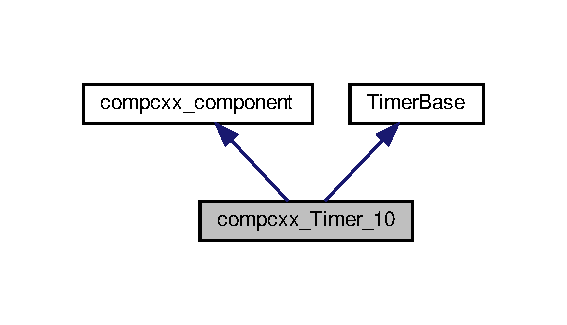
\includegraphics[width=272pt]{classcompcxx__Timer__10__inherit__graph}
\end{center}
\end{figure}


Collaboration diagram for compcxx\+\_\+\+Timer\+\_\+10\+:\nopagebreak
\begin{figure}[H]
\begin{center}
\leavevmode
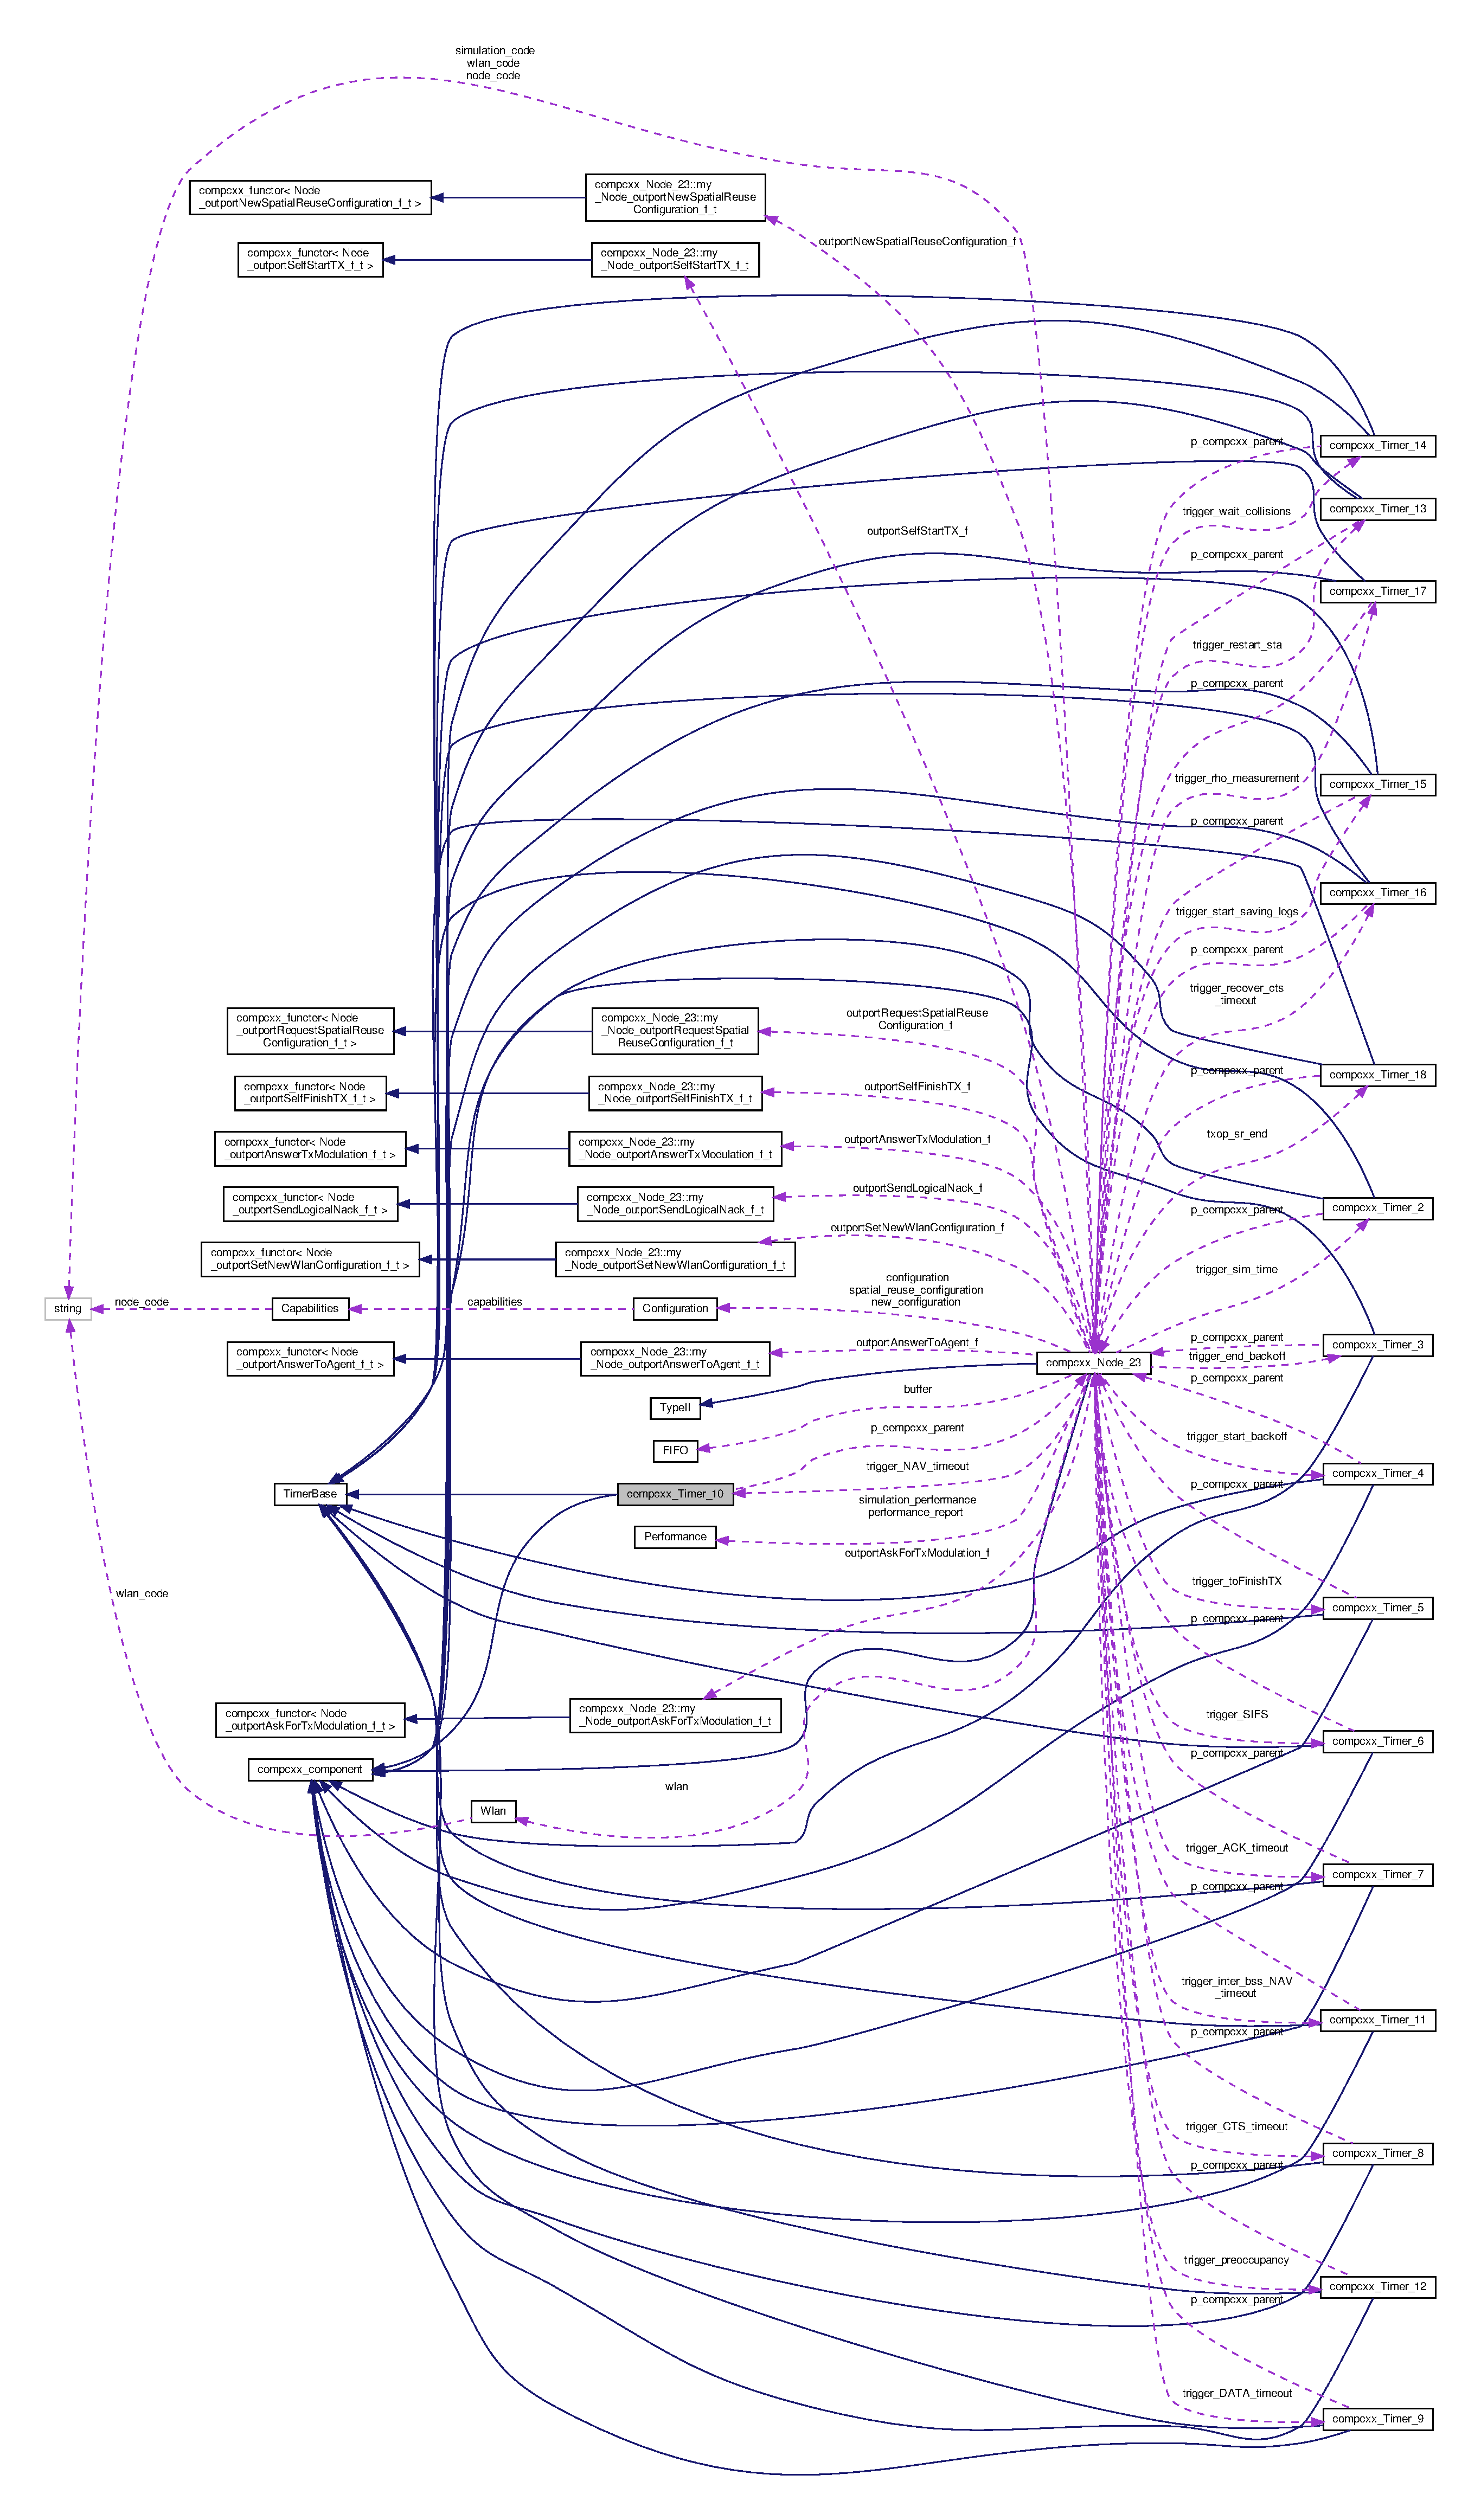
\includegraphics[height=550pt]{classcompcxx__Timer__10__coll__graph}
\end{center}
\end{figure}
\subsection*{Classes}
\begin{DoxyCompactItemize}
\item 
struct \hyperlink{structcompcxx__Timer__10_1_1event__t}{event\+\_\+t}
\end{DoxyCompactItemize}
\subsection*{Public Member Functions}
\begin{DoxyCompactItemize}
\item 
\mbox{\Hypertarget{classcompcxx__Timer__10_a35508eedbf5cb78e053174c44688e6f4}\label{classcompcxx__Timer__10_a35508eedbf5cb78e053174c44688e6f4}} 
void {\bfseries Set} (\hyperlink{classtrigger__t}{trigger\+\_\+t} const \&, double)
\item 
\mbox{\Hypertarget{classcompcxx__Timer__10_a2bf077ea65b8fbc88b3ebf108fbe8da5}\label{classcompcxx__Timer__10_a2bf077ea65b8fbc88b3ebf108fbe8da5}} 
void {\bfseries Set} (double)
\item 
\mbox{\Hypertarget{classcompcxx__Timer__10_a288c157b11c2d645880a21eef3d9b6b8}\label{classcompcxx__Timer__10_a288c157b11c2d645880a21eef3d9b6b8}} 
double {\bfseries Get\+Time} ()
\item 
\mbox{\Hypertarget{classcompcxx__Timer__10_aa809e71aac6092adba0384433f539a5e}\label{classcompcxx__Timer__10_aa809e71aac6092adba0384433f539a5e}} 
bool {\bfseries Active} ()
\item 
\mbox{\Hypertarget{classcompcxx__Timer__10_a1bcedc4e71301faf86b5caf74a1526f4}\label{classcompcxx__Timer__10_a1bcedc4e71301faf86b5caf74a1526f4}} 
\hyperlink{classtrigger__t}{trigger\+\_\+t} \& {\bfseries Get\+Data} ()
\item 
\mbox{\Hypertarget{classcompcxx__Timer__10_ad3c838b97f553dc53928ecec70709676}\label{classcompcxx__Timer__10_ad3c838b97f553dc53928ecec70709676}} 
void {\bfseries Set\+Data} (\hyperlink{classtrigger__t}{trigger\+\_\+t} const \&d)
\item 
\mbox{\Hypertarget{classcompcxx__Timer__10_ac018a4b0291d4e711272c9d37550d1f5}\label{classcompcxx__Timer__10_ac018a4b0291d4e711272c9d37550d1f5}} 
void {\bfseries Cancel} ()
\item 
\mbox{\Hypertarget{classcompcxx__Timer__10_adf1726b38c1e20432a27b582859aff96}\label{classcompcxx__Timer__10_adf1726b38c1e20432a27b582859aff96}} 
void {\bfseries activate} (\hyperlink{structCostEvent}{Cost\+Event} $\ast$)
\end{DoxyCompactItemize}
\subsection*{Public Attributes}
\begin{DoxyCompactItemize}
\item 
\mbox{\Hypertarget{classcompcxx__Timer__10_acde34ceea3d963086acfd1f3ec3cf529}\label{classcompcxx__Timer__10_acde34ceea3d963086acfd1f3ec3cf529}} 
\hyperlink{classcompcxx__Node__23}{compcxx\+\_\+\+Node\+\_\+23} $\ast$ {\bfseries p\+\_\+compcxx\+\_\+parent}
\end{DoxyCompactItemize}
\subsection*{Additional Inherited Members}


The documentation for this class was generated from the following file\+:\begin{DoxyCompactItemize}
\item 
Code/main/komondor\+\_\+main.\+cxx\end{DoxyCompactItemize}

\hypertarget{classcompcxx__Timer__11}{}\section{compcxx\+\_\+\+Timer\+\_\+11 Class Reference}
\label{classcompcxx__Timer__11}\index{compcxx\+\_\+\+Timer\+\_\+11@{compcxx\+\_\+\+Timer\+\_\+11}}


Inheritance diagram for compcxx\+\_\+\+Timer\+\_\+11\+:\nopagebreak
\begin{figure}[H]
\begin{center}
\leavevmode
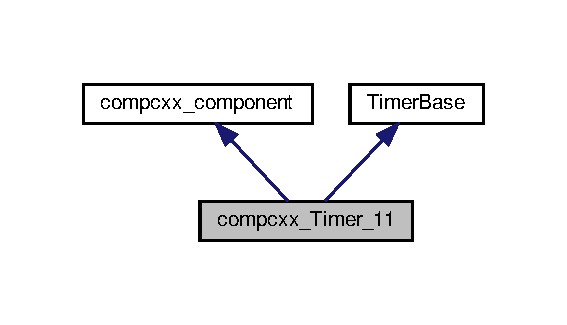
\includegraphics[width=272pt]{classcompcxx__Timer__11__inherit__graph}
\end{center}
\end{figure}


Collaboration diagram for compcxx\+\_\+\+Timer\+\_\+11\+:\nopagebreak
\begin{figure}[H]
\begin{center}
\leavevmode
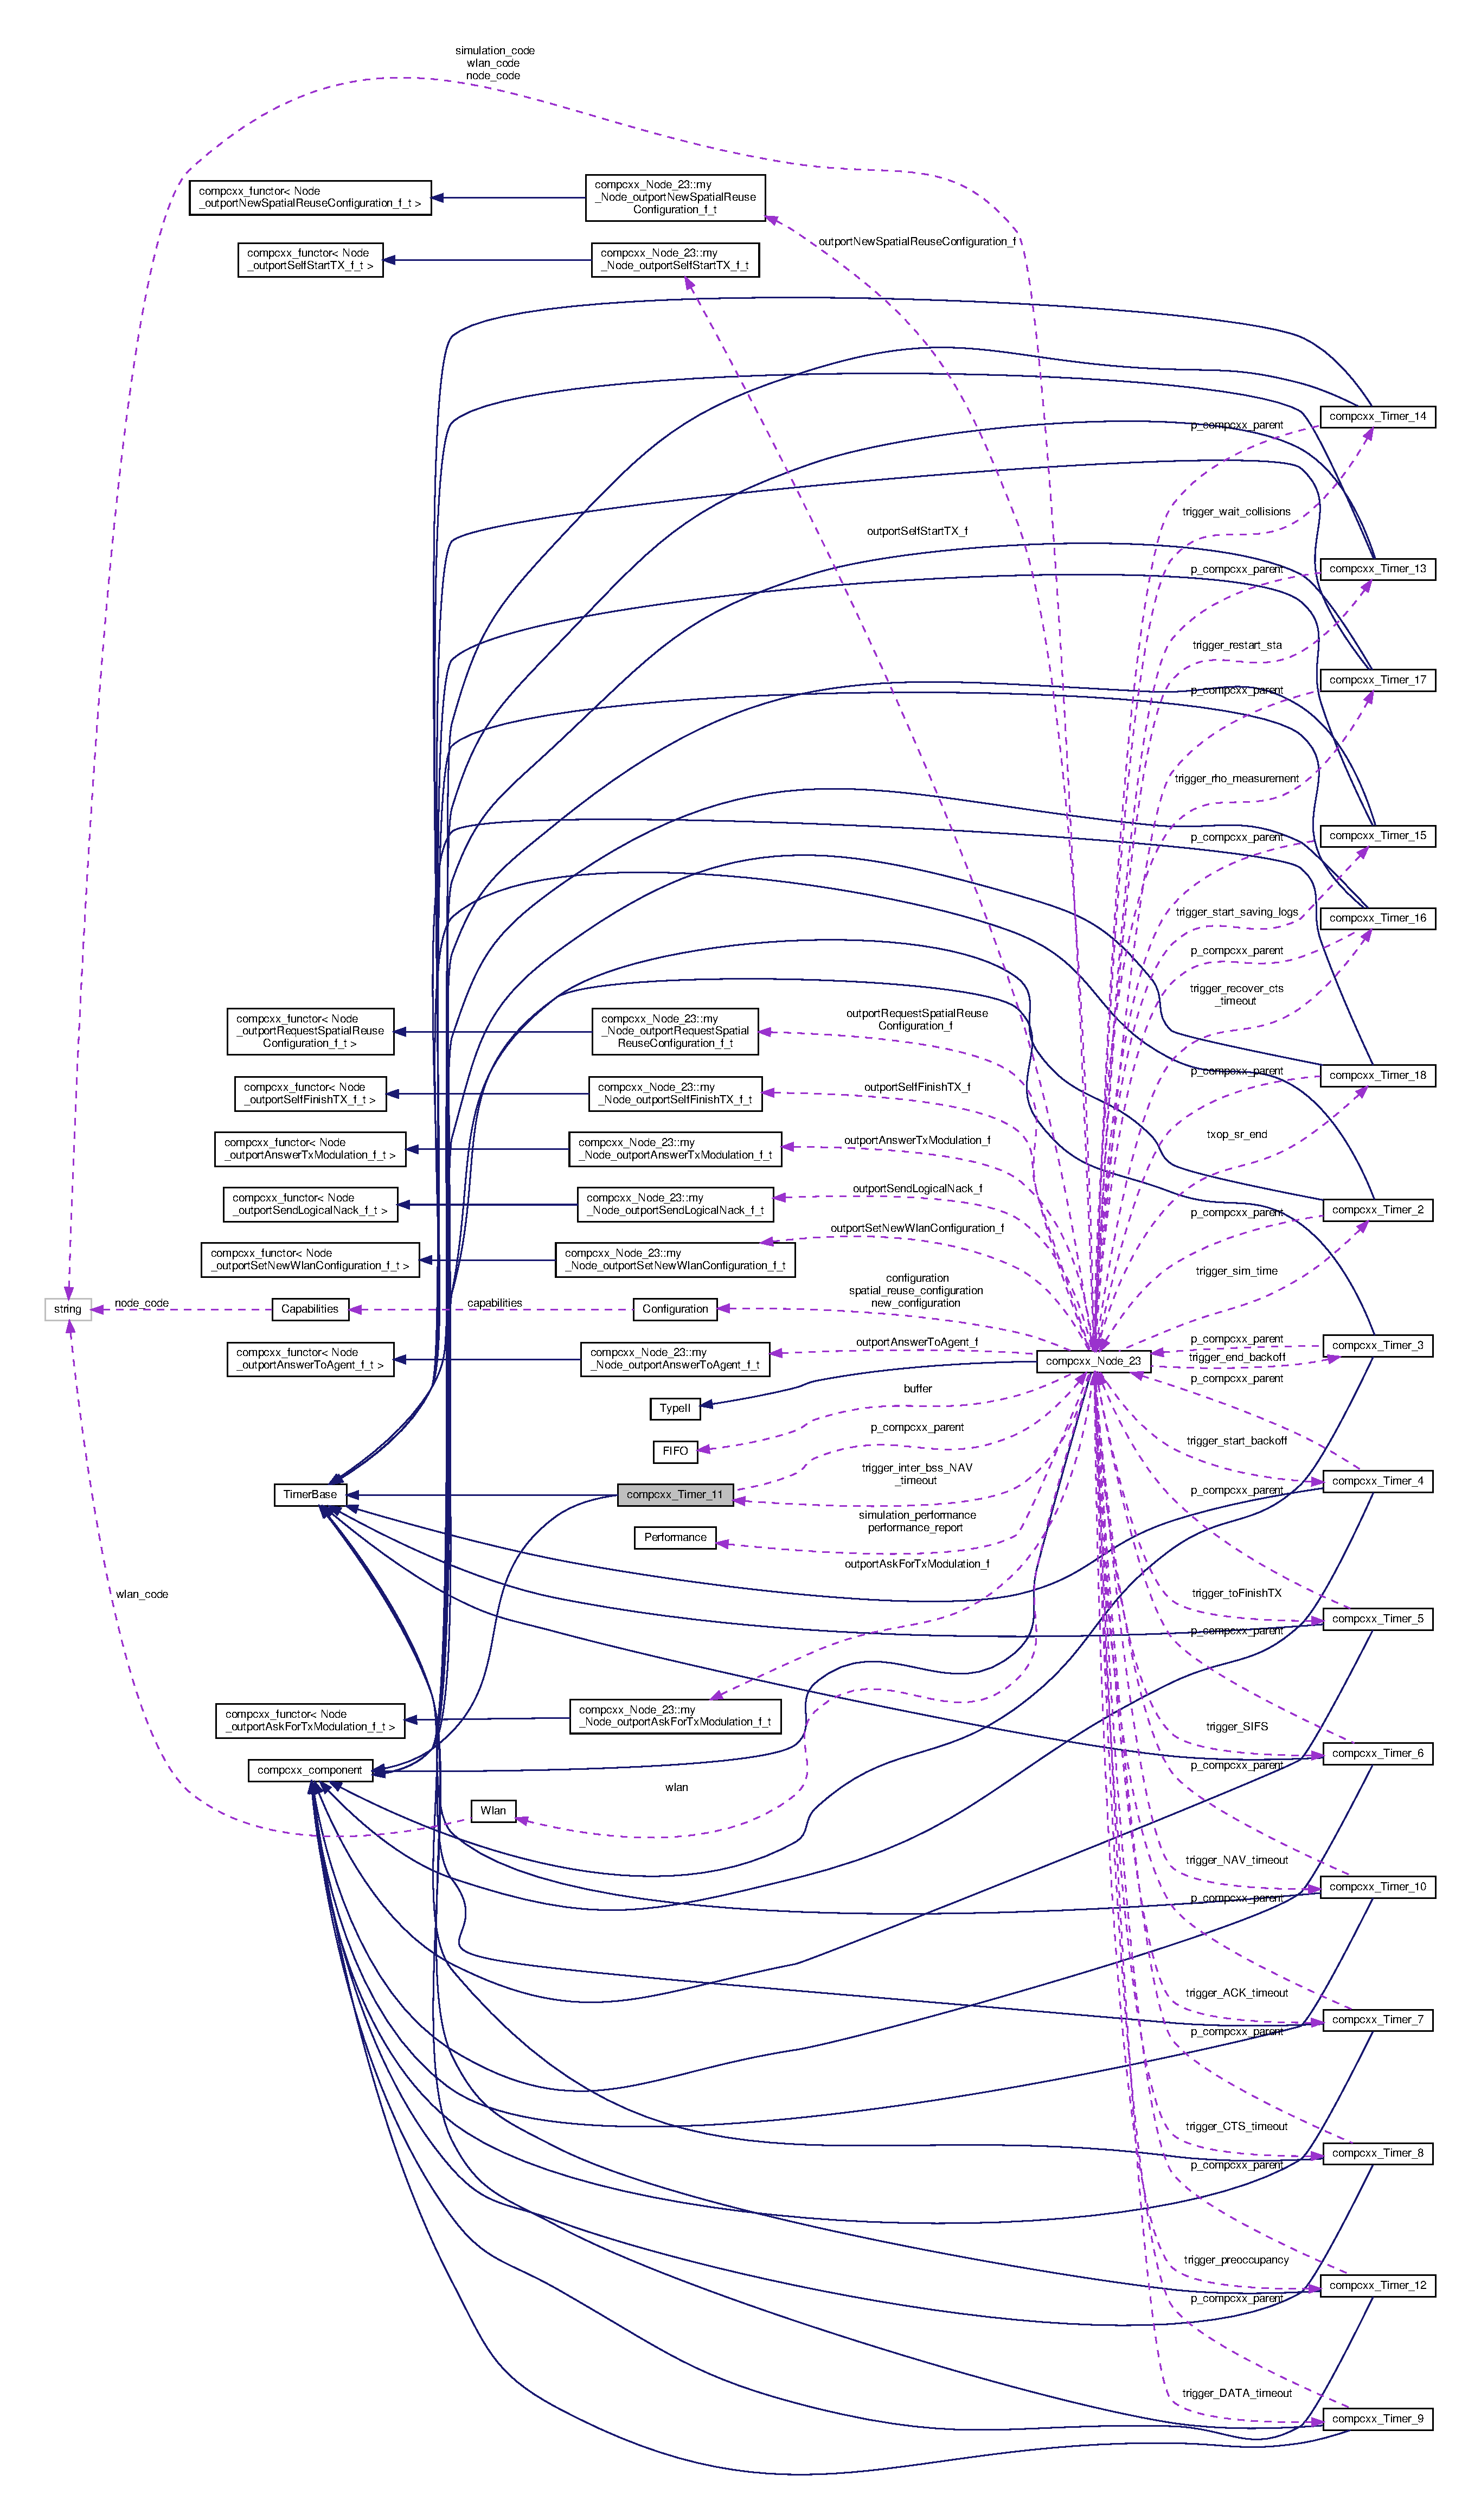
\includegraphics[height=550pt]{classcompcxx__Timer__11__coll__graph}
\end{center}
\end{figure}
\subsection*{Classes}
\begin{DoxyCompactItemize}
\item 
struct \hyperlink{structcompcxx__Timer__11_1_1event__t}{event\+\_\+t}
\end{DoxyCompactItemize}
\subsection*{Public Member Functions}
\begin{DoxyCompactItemize}
\item 
\mbox{\Hypertarget{classcompcxx__Timer__11_a82bdd55619eea9037016467f9ad64fa7}\label{classcompcxx__Timer__11_a82bdd55619eea9037016467f9ad64fa7}} 
void {\bfseries Set} (\hyperlink{classtrigger__t}{trigger\+\_\+t} const \&, double)
\item 
\mbox{\Hypertarget{classcompcxx__Timer__11_a0e911365d422e2b09b29e1cc99c73c8f}\label{classcompcxx__Timer__11_a0e911365d422e2b09b29e1cc99c73c8f}} 
void {\bfseries Set} (double)
\item 
\mbox{\Hypertarget{classcompcxx__Timer__11_a47d4f9862ba24b95f11378bfd1d72f35}\label{classcompcxx__Timer__11_a47d4f9862ba24b95f11378bfd1d72f35}} 
double {\bfseries Get\+Time} ()
\item 
\mbox{\Hypertarget{classcompcxx__Timer__11_a8e81be419f1f85353ece43a88f9c07c9}\label{classcompcxx__Timer__11_a8e81be419f1f85353ece43a88f9c07c9}} 
bool {\bfseries Active} ()
\item 
\mbox{\Hypertarget{classcompcxx__Timer__11_ac033d35735807699b0ba0ebedd19e592}\label{classcompcxx__Timer__11_ac033d35735807699b0ba0ebedd19e592}} 
\hyperlink{classtrigger__t}{trigger\+\_\+t} \& {\bfseries Get\+Data} ()
\item 
\mbox{\Hypertarget{classcompcxx__Timer__11_af87593fee948e3b729a4f33022d0a4aa}\label{classcompcxx__Timer__11_af87593fee948e3b729a4f33022d0a4aa}} 
void {\bfseries Set\+Data} (\hyperlink{classtrigger__t}{trigger\+\_\+t} const \&d)
\item 
\mbox{\Hypertarget{classcompcxx__Timer__11_a0f0cdd6bd30b906b4c024f8e3388962a}\label{classcompcxx__Timer__11_a0f0cdd6bd30b906b4c024f8e3388962a}} 
void {\bfseries Cancel} ()
\item 
\mbox{\Hypertarget{classcompcxx__Timer__11_ad24dc6301d30aa582e83e8185e78f773}\label{classcompcxx__Timer__11_ad24dc6301d30aa582e83e8185e78f773}} 
void {\bfseries activate} (\hyperlink{structCostEvent}{Cost\+Event} $\ast$)
\end{DoxyCompactItemize}
\subsection*{Public Attributes}
\begin{DoxyCompactItemize}
\item 
\mbox{\Hypertarget{classcompcxx__Timer__11_ae113b494ff858f0b6508e464bfd9500e}\label{classcompcxx__Timer__11_ae113b494ff858f0b6508e464bfd9500e}} 
\hyperlink{classcompcxx__Node__23}{compcxx\+\_\+\+Node\+\_\+23} $\ast$ {\bfseries p\+\_\+compcxx\+\_\+parent}
\end{DoxyCompactItemize}
\subsection*{Additional Inherited Members}


The documentation for this class was generated from the following file\+:\begin{DoxyCompactItemize}
\item 
Code/main/komondor\+\_\+main.\+cxx\end{DoxyCompactItemize}

\hypertarget{classcompcxx__Timer__12}{}\section{compcxx\+\_\+\+Timer\+\_\+12 Class Reference}
\label{classcompcxx__Timer__12}\index{compcxx\+\_\+\+Timer\+\_\+12@{compcxx\+\_\+\+Timer\+\_\+12}}


Inheritance diagram for compcxx\+\_\+\+Timer\+\_\+12\+:\nopagebreak
\begin{figure}[H]
\begin{center}
\leavevmode
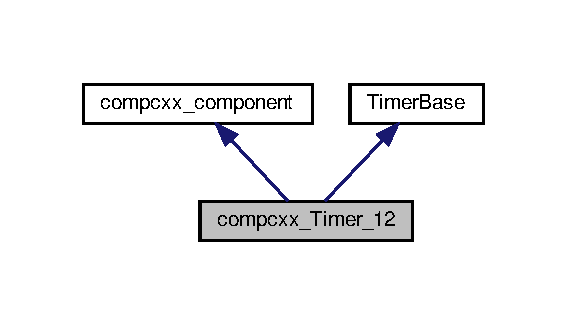
\includegraphics[width=272pt]{classcompcxx__Timer__12__inherit__graph}
\end{center}
\end{figure}


Collaboration diagram for compcxx\+\_\+\+Timer\+\_\+12\+:\nopagebreak
\begin{figure}[H]
\begin{center}
\leavevmode
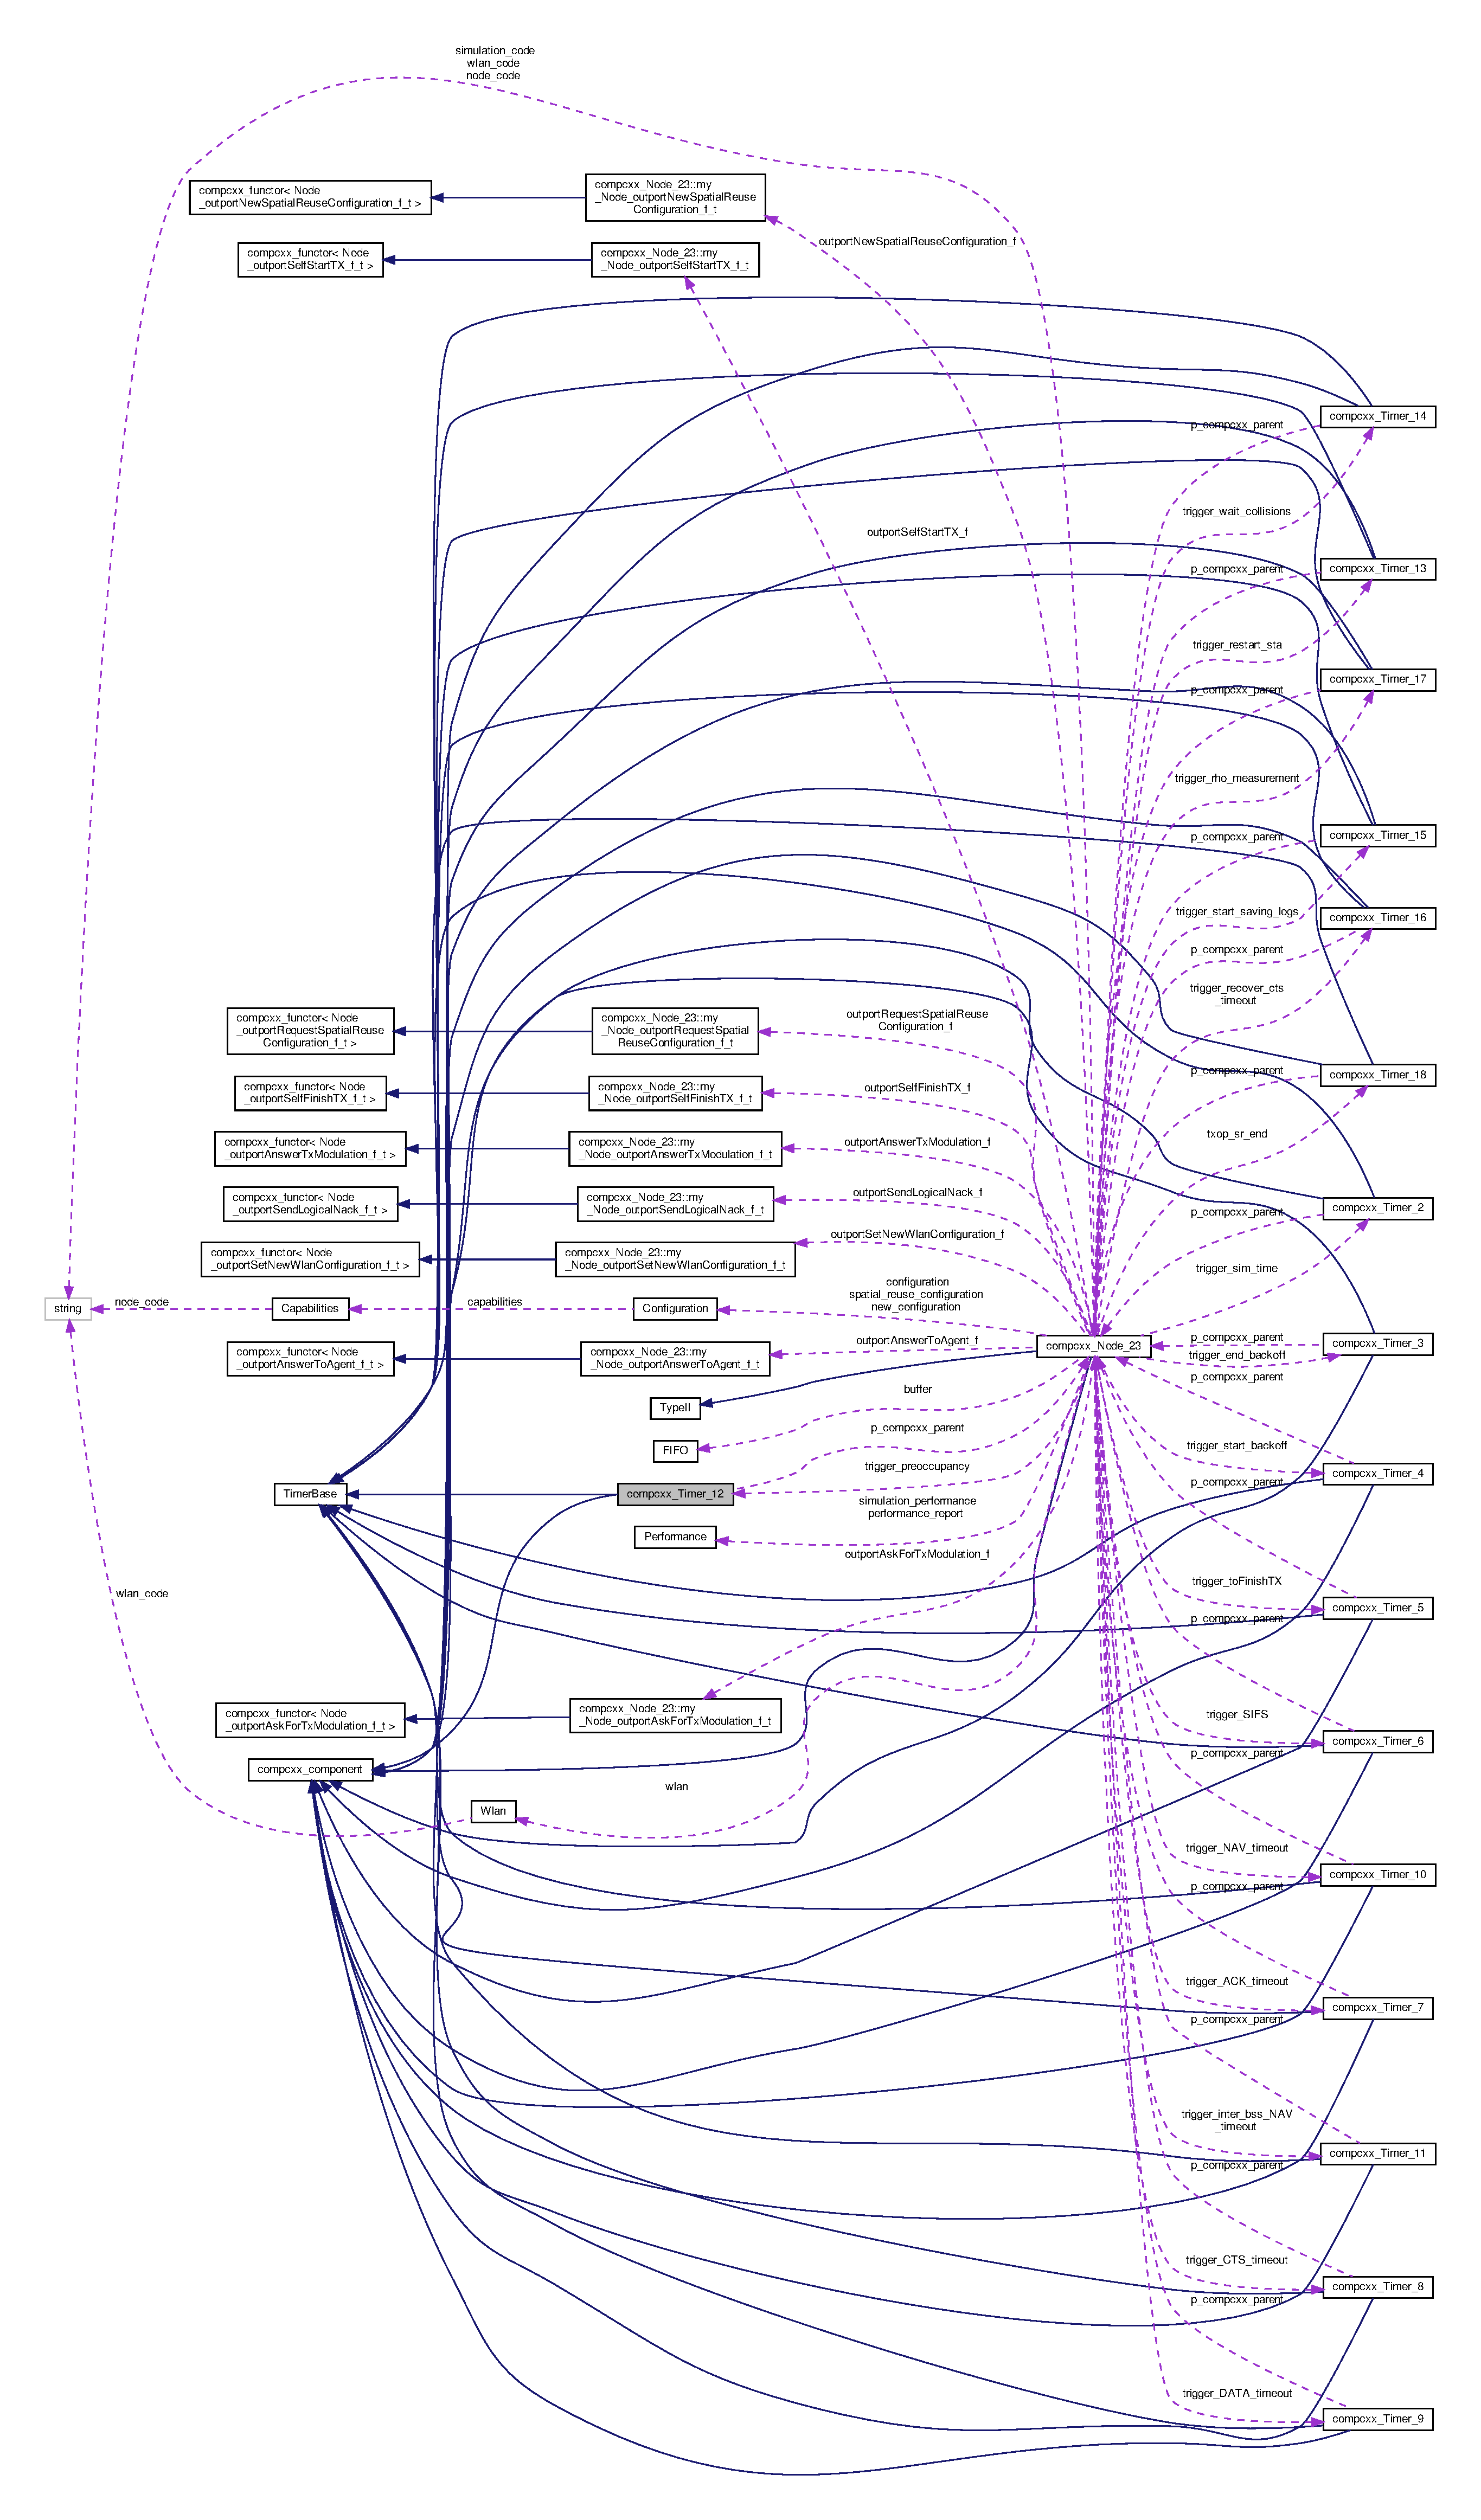
\includegraphics[height=550pt]{classcompcxx__Timer__12__coll__graph}
\end{center}
\end{figure}
\subsection*{Classes}
\begin{DoxyCompactItemize}
\item 
struct \hyperlink{structcompcxx__Timer__12_1_1event__t}{event\+\_\+t}
\end{DoxyCompactItemize}
\subsection*{Public Member Functions}
\begin{DoxyCompactItemize}
\item 
\mbox{\Hypertarget{classcompcxx__Timer__12_a48c439bb0ea4456dfe87bae9aeb41aed}\label{classcompcxx__Timer__12_a48c439bb0ea4456dfe87bae9aeb41aed}} 
void {\bfseries Set} (\hyperlink{classtrigger__t}{trigger\+\_\+t} const \&, double)
\item 
\mbox{\Hypertarget{classcompcxx__Timer__12_a8f65f60c7bb5e920522a16f80c5d3761}\label{classcompcxx__Timer__12_a8f65f60c7bb5e920522a16f80c5d3761}} 
void {\bfseries Set} (double)
\item 
\mbox{\Hypertarget{classcompcxx__Timer__12_a259e4cf89b8a923668ca108896ab31e0}\label{classcompcxx__Timer__12_a259e4cf89b8a923668ca108896ab31e0}} 
double {\bfseries Get\+Time} ()
\item 
\mbox{\Hypertarget{classcompcxx__Timer__12_a7d0b4086854652ce65824bdc76e5d4b4}\label{classcompcxx__Timer__12_a7d0b4086854652ce65824bdc76e5d4b4}} 
bool {\bfseries Active} ()
\item 
\mbox{\Hypertarget{classcompcxx__Timer__12_aad6219ba02b96873970bc5a4b7b15d24}\label{classcompcxx__Timer__12_aad6219ba02b96873970bc5a4b7b15d24}} 
\hyperlink{classtrigger__t}{trigger\+\_\+t} \& {\bfseries Get\+Data} ()
\item 
\mbox{\Hypertarget{classcompcxx__Timer__12_a36b3814adb8c45b5eb740ea6aa725ef8}\label{classcompcxx__Timer__12_a36b3814adb8c45b5eb740ea6aa725ef8}} 
void {\bfseries Set\+Data} (\hyperlink{classtrigger__t}{trigger\+\_\+t} const \&d)
\item 
\mbox{\Hypertarget{classcompcxx__Timer__12_a4afe3ca3657597eee3bda74f093da55f}\label{classcompcxx__Timer__12_a4afe3ca3657597eee3bda74f093da55f}} 
void {\bfseries Cancel} ()
\item 
\mbox{\Hypertarget{classcompcxx__Timer__12_a51eb4e6c0e30da77213d0f4b4270e922}\label{classcompcxx__Timer__12_a51eb4e6c0e30da77213d0f4b4270e922}} 
void {\bfseries activate} (\hyperlink{structCostEvent}{Cost\+Event} $\ast$)
\end{DoxyCompactItemize}
\subsection*{Public Attributes}
\begin{DoxyCompactItemize}
\item 
\mbox{\Hypertarget{classcompcxx__Timer__12_a4483d6a556154e637b196856fef74e2e}\label{classcompcxx__Timer__12_a4483d6a556154e637b196856fef74e2e}} 
\hyperlink{classcompcxx__Node__23}{compcxx\+\_\+\+Node\+\_\+23} $\ast$ {\bfseries p\+\_\+compcxx\+\_\+parent}
\end{DoxyCompactItemize}
\subsection*{Additional Inherited Members}


The documentation for this class was generated from the following file\+:\begin{DoxyCompactItemize}
\item 
Code/main/komondor\+\_\+main.\+cxx\end{DoxyCompactItemize}

\hypertarget{classcompcxx__Timer__13}{}\section{compcxx\+\_\+\+Timer\+\_\+13 Class Reference}
\label{classcompcxx__Timer__13}\index{compcxx\+\_\+\+Timer\+\_\+13@{compcxx\+\_\+\+Timer\+\_\+13}}


Inheritance diagram for compcxx\+\_\+\+Timer\+\_\+13\+:\nopagebreak
\begin{figure}[H]
\begin{center}
\leavevmode
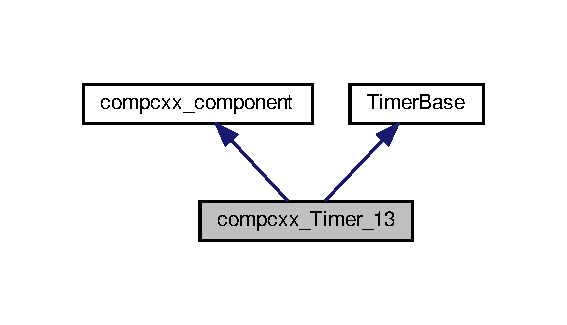
\includegraphics[width=272pt]{classcompcxx__Timer__13__inherit__graph}
\end{center}
\end{figure}


Collaboration diagram for compcxx\+\_\+\+Timer\+\_\+13\+:\nopagebreak
\begin{figure}[H]
\begin{center}
\leavevmode
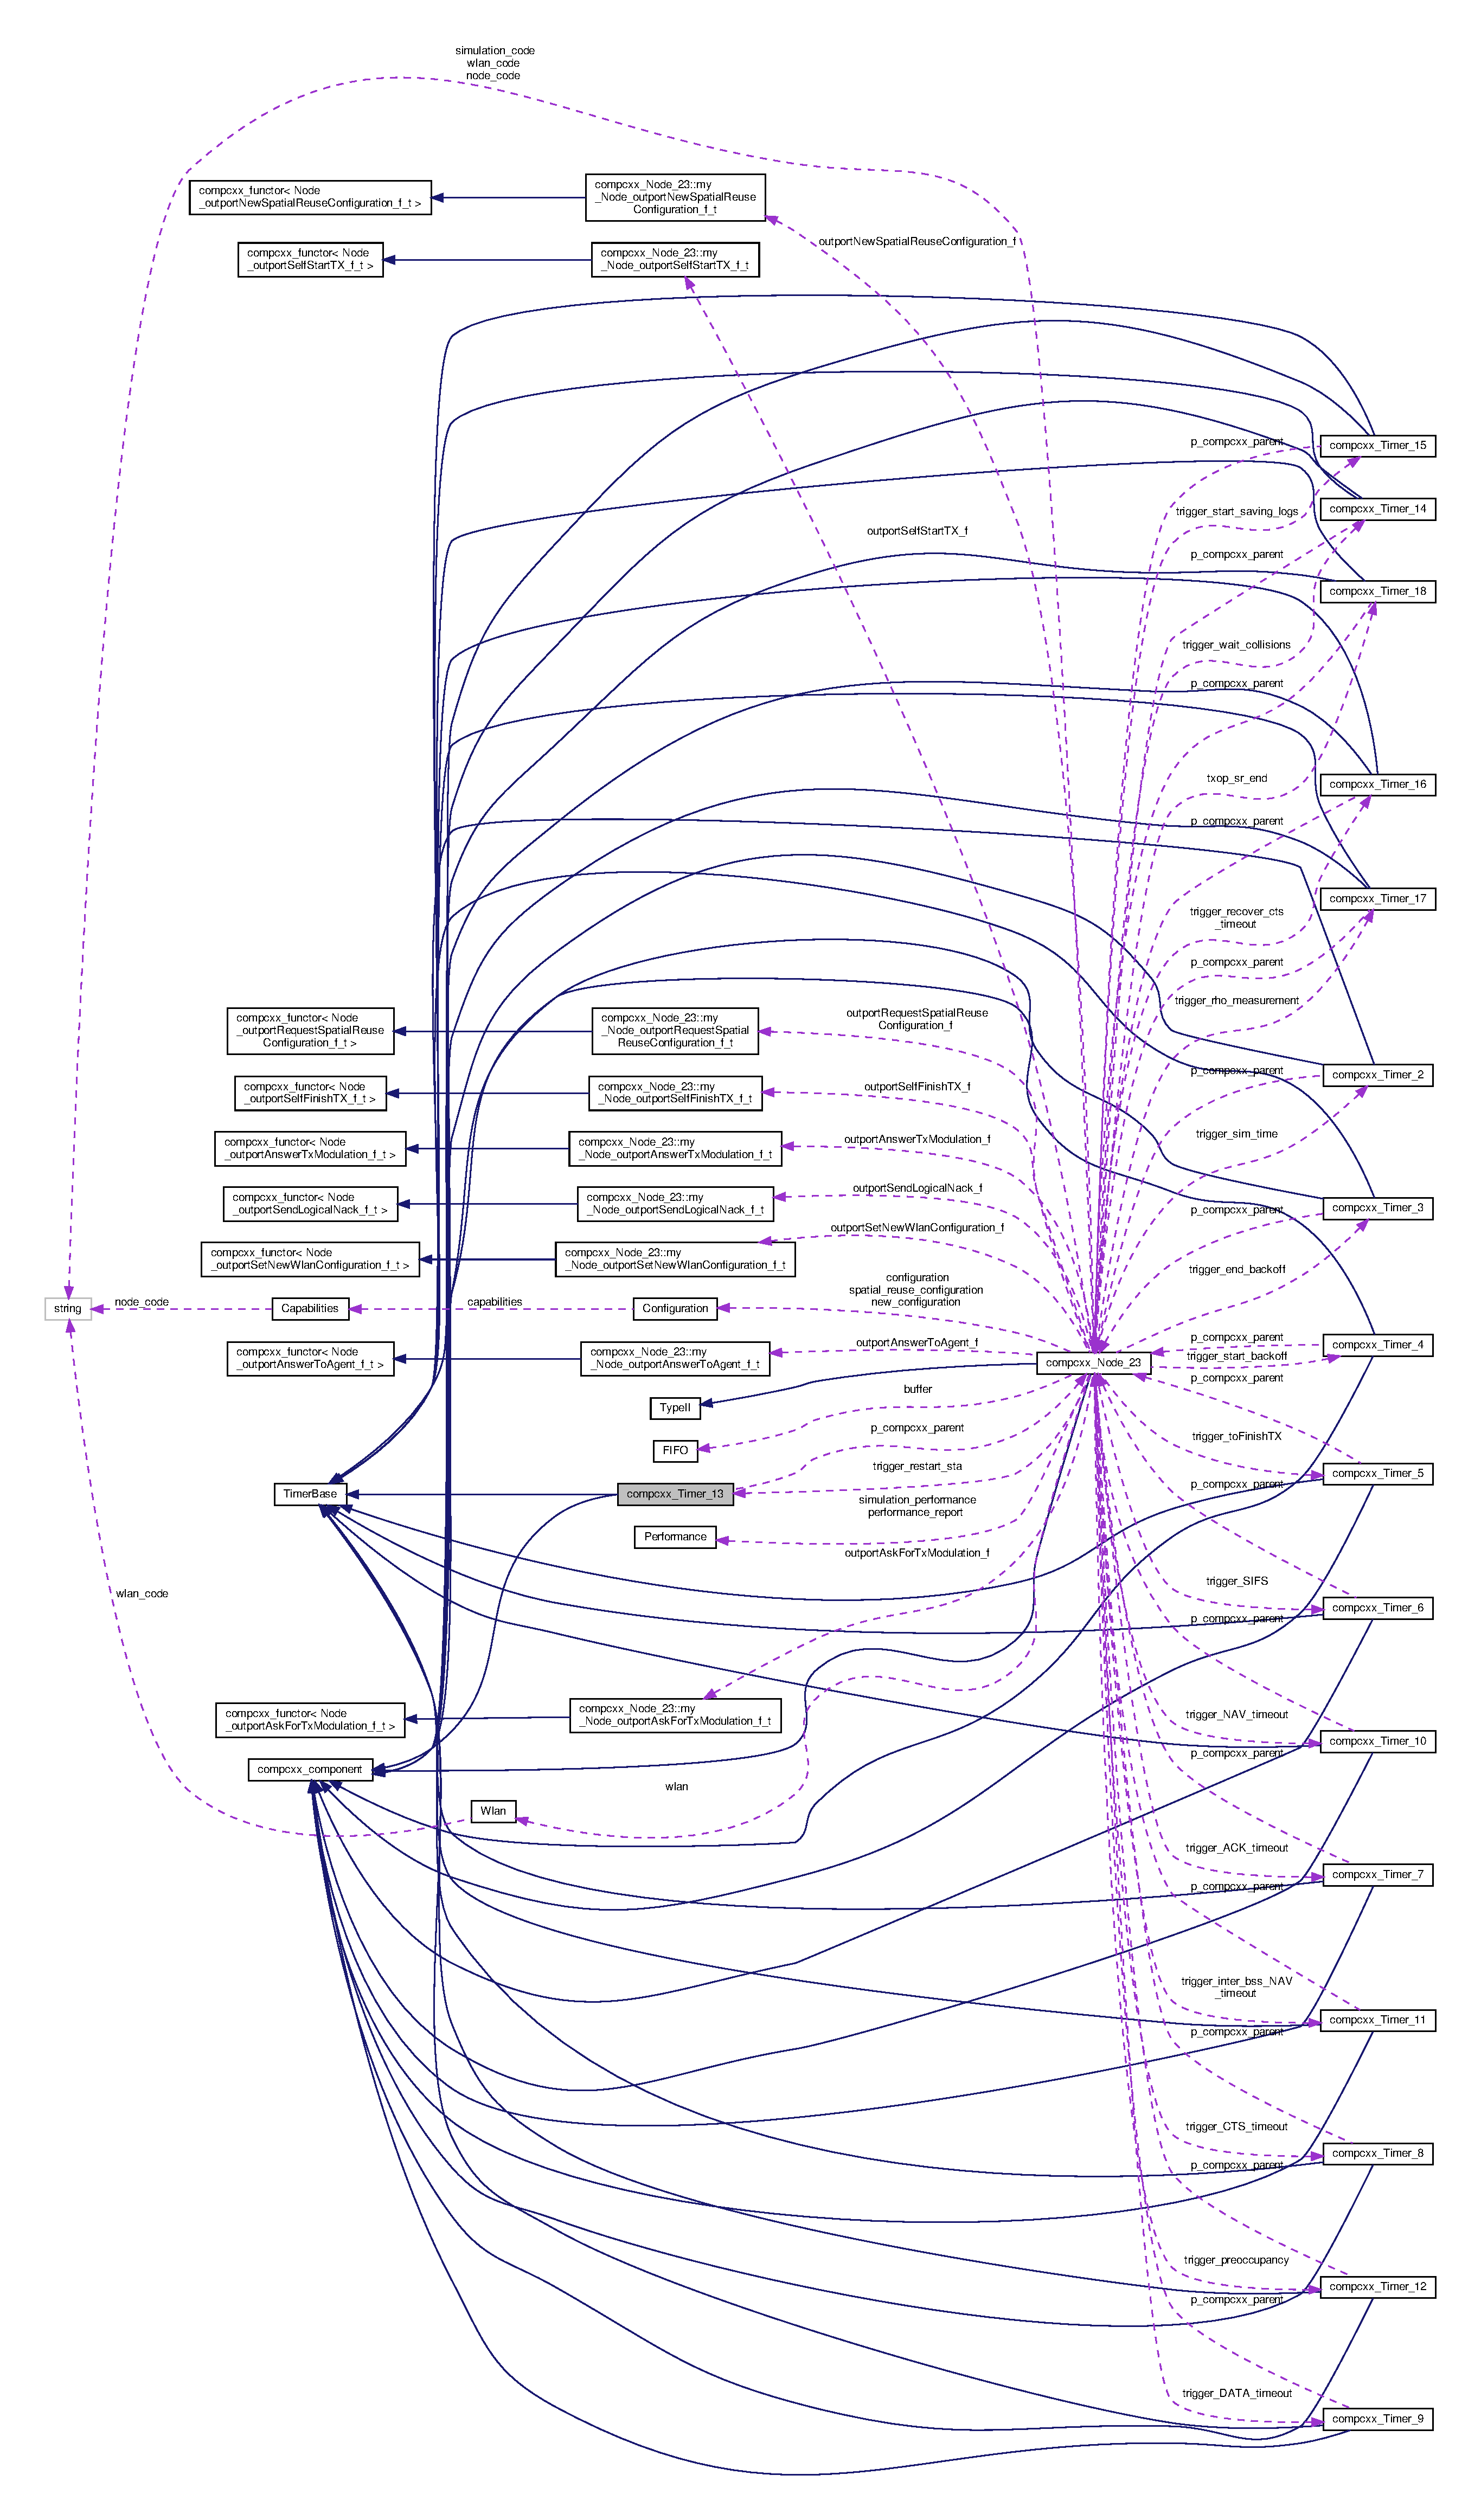
\includegraphics[height=550pt]{classcompcxx__Timer__13__coll__graph}
\end{center}
\end{figure}
\subsection*{Classes}
\begin{DoxyCompactItemize}
\item 
struct \hyperlink{structcompcxx__Timer__13_1_1event__t}{event\+\_\+t}
\end{DoxyCompactItemize}
\subsection*{Public Member Functions}
\begin{DoxyCompactItemize}
\item 
\mbox{\Hypertarget{classcompcxx__Timer__13_afdb73ad23b0fbb8822bfc053703e6d39}\label{classcompcxx__Timer__13_afdb73ad23b0fbb8822bfc053703e6d39}} 
void {\bfseries Set} (\hyperlink{classtrigger__t}{trigger\+\_\+t} const \&, double)
\item 
\mbox{\Hypertarget{classcompcxx__Timer__13_a7a78fe965b2aaf0892c1e46bfc87e708}\label{classcompcxx__Timer__13_a7a78fe965b2aaf0892c1e46bfc87e708}} 
void {\bfseries Set} (double)
\item 
\mbox{\Hypertarget{classcompcxx__Timer__13_aac59f428417ee7fd05098292998f4d5e}\label{classcompcxx__Timer__13_aac59f428417ee7fd05098292998f4d5e}} 
double {\bfseries Get\+Time} ()
\item 
\mbox{\Hypertarget{classcompcxx__Timer__13_a95f3ccb491c044f057052bcd5e548a6c}\label{classcompcxx__Timer__13_a95f3ccb491c044f057052bcd5e548a6c}} 
bool {\bfseries Active} ()
\item 
\mbox{\Hypertarget{classcompcxx__Timer__13_a091b9ca4b3fbd1d333411c2482d6e966}\label{classcompcxx__Timer__13_a091b9ca4b3fbd1d333411c2482d6e966}} 
\hyperlink{classtrigger__t}{trigger\+\_\+t} \& {\bfseries Get\+Data} ()
\item 
\mbox{\Hypertarget{classcompcxx__Timer__13_a187c82120af18a182a60e5689d7e5061}\label{classcompcxx__Timer__13_a187c82120af18a182a60e5689d7e5061}} 
void {\bfseries Set\+Data} (\hyperlink{classtrigger__t}{trigger\+\_\+t} const \&d)
\item 
\mbox{\Hypertarget{classcompcxx__Timer__13_a92fbe585c459d0c32b927d717538ce25}\label{classcompcxx__Timer__13_a92fbe585c459d0c32b927d717538ce25}} 
void {\bfseries Cancel} ()
\item 
\mbox{\Hypertarget{classcompcxx__Timer__13_aa792f020ca6e409f490130582217fefb}\label{classcompcxx__Timer__13_aa792f020ca6e409f490130582217fefb}} 
void {\bfseries activate} (\hyperlink{structCostEvent}{Cost\+Event} $\ast$)
\end{DoxyCompactItemize}
\subsection*{Public Attributes}
\begin{DoxyCompactItemize}
\item 
\mbox{\Hypertarget{classcompcxx__Timer__13_a1ee889c8bfd9c75dfd897aa3d401df0f}\label{classcompcxx__Timer__13_a1ee889c8bfd9c75dfd897aa3d401df0f}} 
\hyperlink{classcompcxx__Node__23}{compcxx\+\_\+\+Node\+\_\+23} $\ast$ {\bfseries p\+\_\+compcxx\+\_\+parent}
\end{DoxyCompactItemize}
\subsection*{Additional Inherited Members}


The documentation for this class was generated from the following file\+:\begin{DoxyCompactItemize}
\item 
Code/main/komondor\+\_\+main.\+cxx\end{DoxyCompactItemize}

\hypertarget{classcompcxx__Timer__14}{}\section{compcxx\+\_\+\+Timer\+\_\+14 Class Reference}
\label{classcompcxx__Timer__14}\index{compcxx\+\_\+\+Timer\+\_\+14@{compcxx\+\_\+\+Timer\+\_\+14}}


Inheritance diagram for compcxx\+\_\+\+Timer\+\_\+14\+:\nopagebreak
\begin{figure}[H]
\begin{center}
\leavevmode
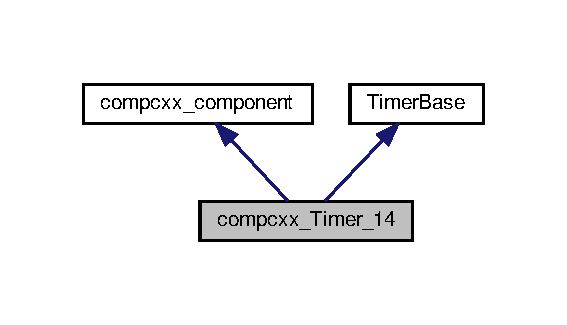
\includegraphics[width=272pt]{classcompcxx__Timer__14__inherit__graph}
\end{center}
\end{figure}


Collaboration diagram for compcxx\+\_\+\+Timer\+\_\+14\+:\nopagebreak
\begin{figure}[H]
\begin{center}
\leavevmode
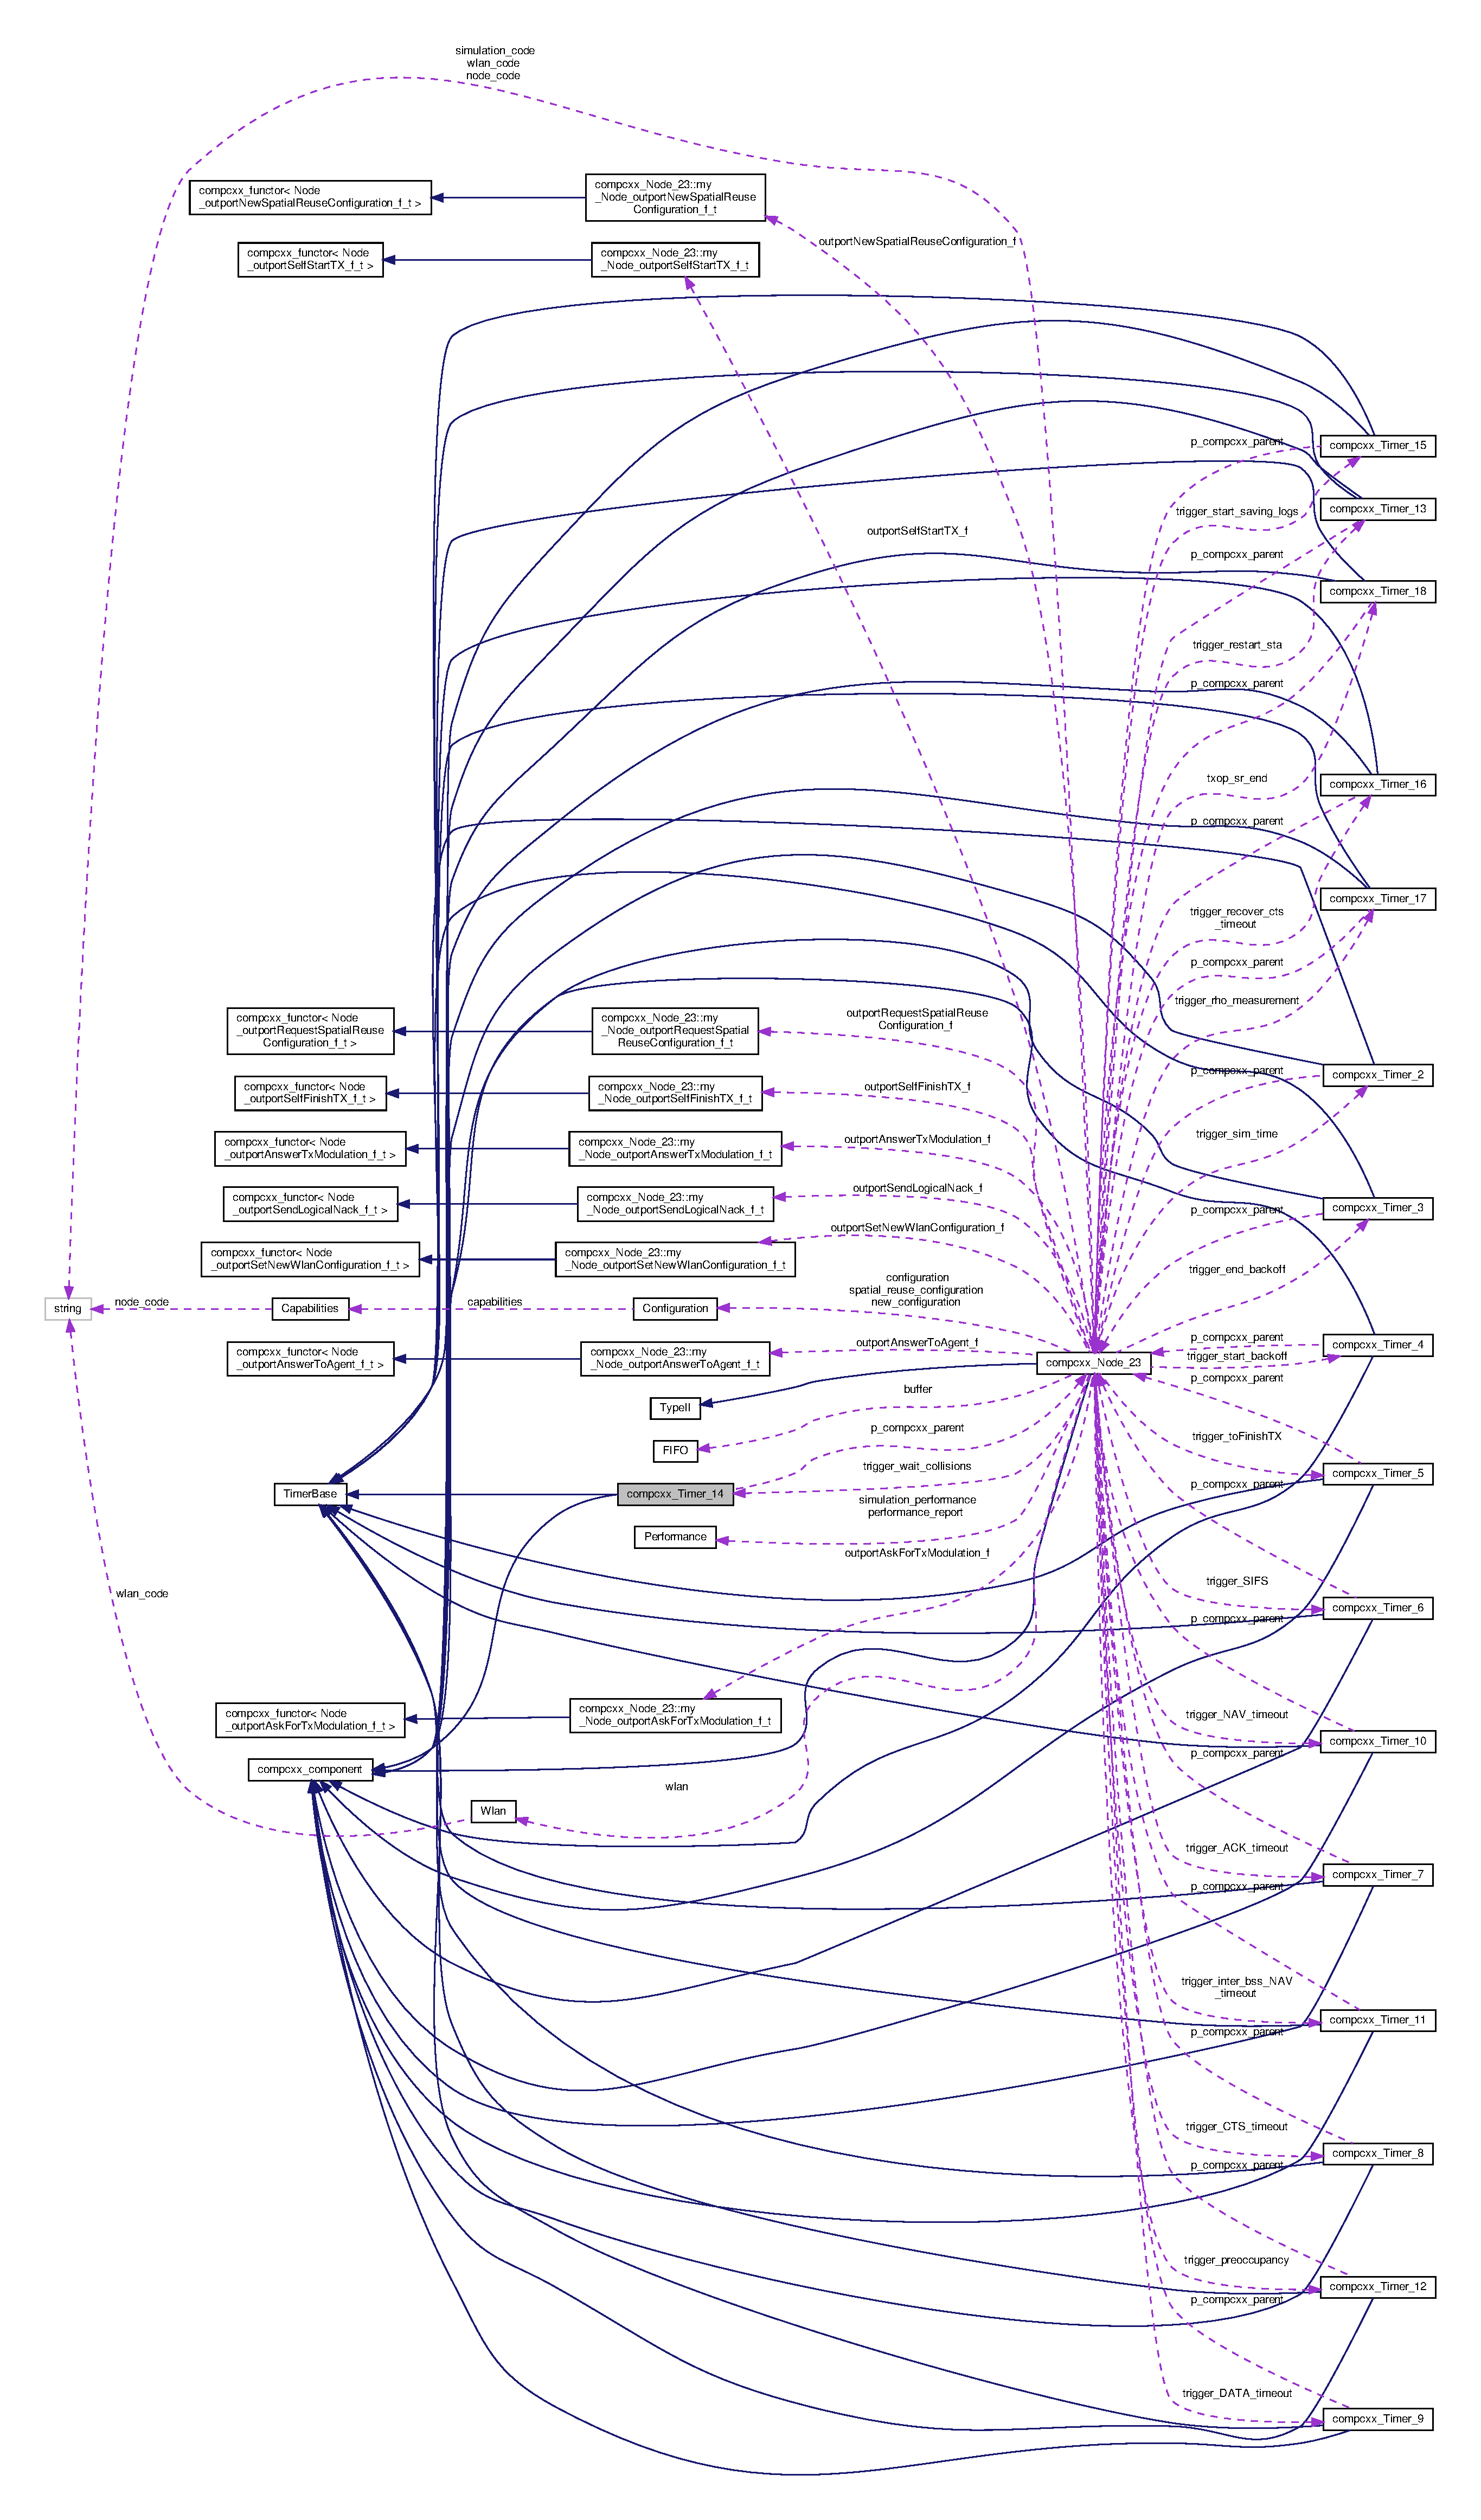
\includegraphics[height=550pt]{classcompcxx__Timer__14__coll__graph}
\end{center}
\end{figure}
\subsection*{Classes}
\begin{DoxyCompactItemize}
\item 
struct \hyperlink{structcompcxx__Timer__14_1_1event__t}{event\+\_\+t}
\end{DoxyCompactItemize}
\subsection*{Public Member Functions}
\begin{DoxyCompactItemize}
\item 
\mbox{\Hypertarget{classcompcxx__Timer__14_a228451cbdbfee1c4224cc2f5f36fcb8f}\label{classcompcxx__Timer__14_a228451cbdbfee1c4224cc2f5f36fcb8f}} 
void {\bfseries Set} (\hyperlink{classtrigger__t}{trigger\+\_\+t} const \&, double)
\item 
\mbox{\Hypertarget{classcompcxx__Timer__14_ae4a5967f1abc06c6a5c327bffd3b2dd2}\label{classcompcxx__Timer__14_ae4a5967f1abc06c6a5c327bffd3b2dd2}} 
void {\bfseries Set} (double)
\item 
\mbox{\Hypertarget{classcompcxx__Timer__14_a8886c3b2f2dd8bf557bde83fb6d9359c}\label{classcompcxx__Timer__14_a8886c3b2f2dd8bf557bde83fb6d9359c}} 
double {\bfseries Get\+Time} ()
\item 
\mbox{\Hypertarget{classcompcxx__Timer__14_a12845ce4638f80272c648f85aa72d72c}\label{classcompcxx__Timer__14_a12845ce4638f80272c648f85aa72d72c}} 
bool {\bfseries Active} ()
\item 
\mbox{\Hypertarget{classcompcxx__Timer__14_adecdc99c62cf310493ec32a9e99f9e74}\label{classcompcxx__Timer__14_adecdc99c62cf310493ec32a9e99f9e74}} 
\hyperlink{classtrigger__t}{trigger\+\_\+t} \& {\bfseries Get\+Data} ()
\item 
\mbox{\Hypertarget{classcompcxx__Timer__14_a12b6b27e4e51e390be78b52fcbb98251}\label{classcompcxx__Timer__14_a12b6b27e4e51e390be78b52fcbb98251}} 
void {\bfseries Set\+Data} (\hyperlink{classtrigger__t}{trigger\+\_\+t} const \&d)
\item 
\mbox{\Hypertarget{classcompcxx__Timer__14_a42a90d53532ed31a0df42370e2352008}\label{classcompcxx__Timer__14_a42a90d53532ed31a0df42370e2352008}} 
void {\bfseries Cancel} ()
\item 
\mbox{\Hypertarget{classcompcxx__Timer__14_a22e97e2c2d6880963798293f46674160}\label{classcompcxx__Timer__14_a22e97e2c2d6880963798293f46674160}} 
void {\bfseries activate} (\hyperlink{structCostEvent}{Cost\+Event} $\ast$)
\end{DoxyCompactItemize}
\subsection*{Public Attributes}
\begin{DoxyCompactItemize}
\item 
\mbox{\Hypertarget{classcompcxx__Timer__14_a0e8abea22c3120fc6f7981a7cf67d133}\label{classcompcxx__Timer__14_a0e8abea22c3120fc6f7981a7cf67d133}} 
\hyperlink{classcompcxx__Node__23}{compcxx\+\_\+\+Node\+\_\+23} $\ast$ {\bfseries p\+\_\+compcxx\+\_\+parent}
\end{DoxyCompactItemize}
\subsection*{Additional Inherited Members}


The documentation for this class was generated from the following file\+:\begin{DoxyCompactItemize}
\item 
Code/main/komondor\+\_\+main.\+cxx\end{DoxyCompactItemize}

\hypertarget{classcompcxx__Timer__15}{}\section{compcxx\+\_\+\+Timer\+\_\+15 Class Reference}
\label{classcompcxx__Timer__15}\index{compcxx\+\_\+\+Timer\+\_\+15@{compcxx\+\_\+\+Timer\+\_\+15}}


Inheritance diagram for compcxx\+\_\+\+Timer\+\_\+15\+:\nopagebreak
\begin{figure}[H]
\begin{center}
\leavevmode
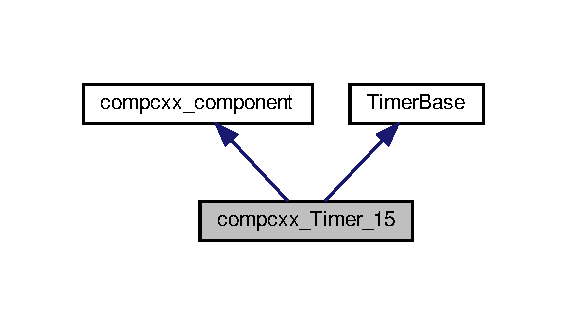
\includegraphics[width=272pt]{classcompcxx__Timer__15__inherit__graph}
\end{center}
\end{figure}


Collaboration diagram for compcxx\+\_\+\+Timer\+\_\+15\+:\nopagebreak
\begin{figure}[H]
\begin{center}
\leavevmode
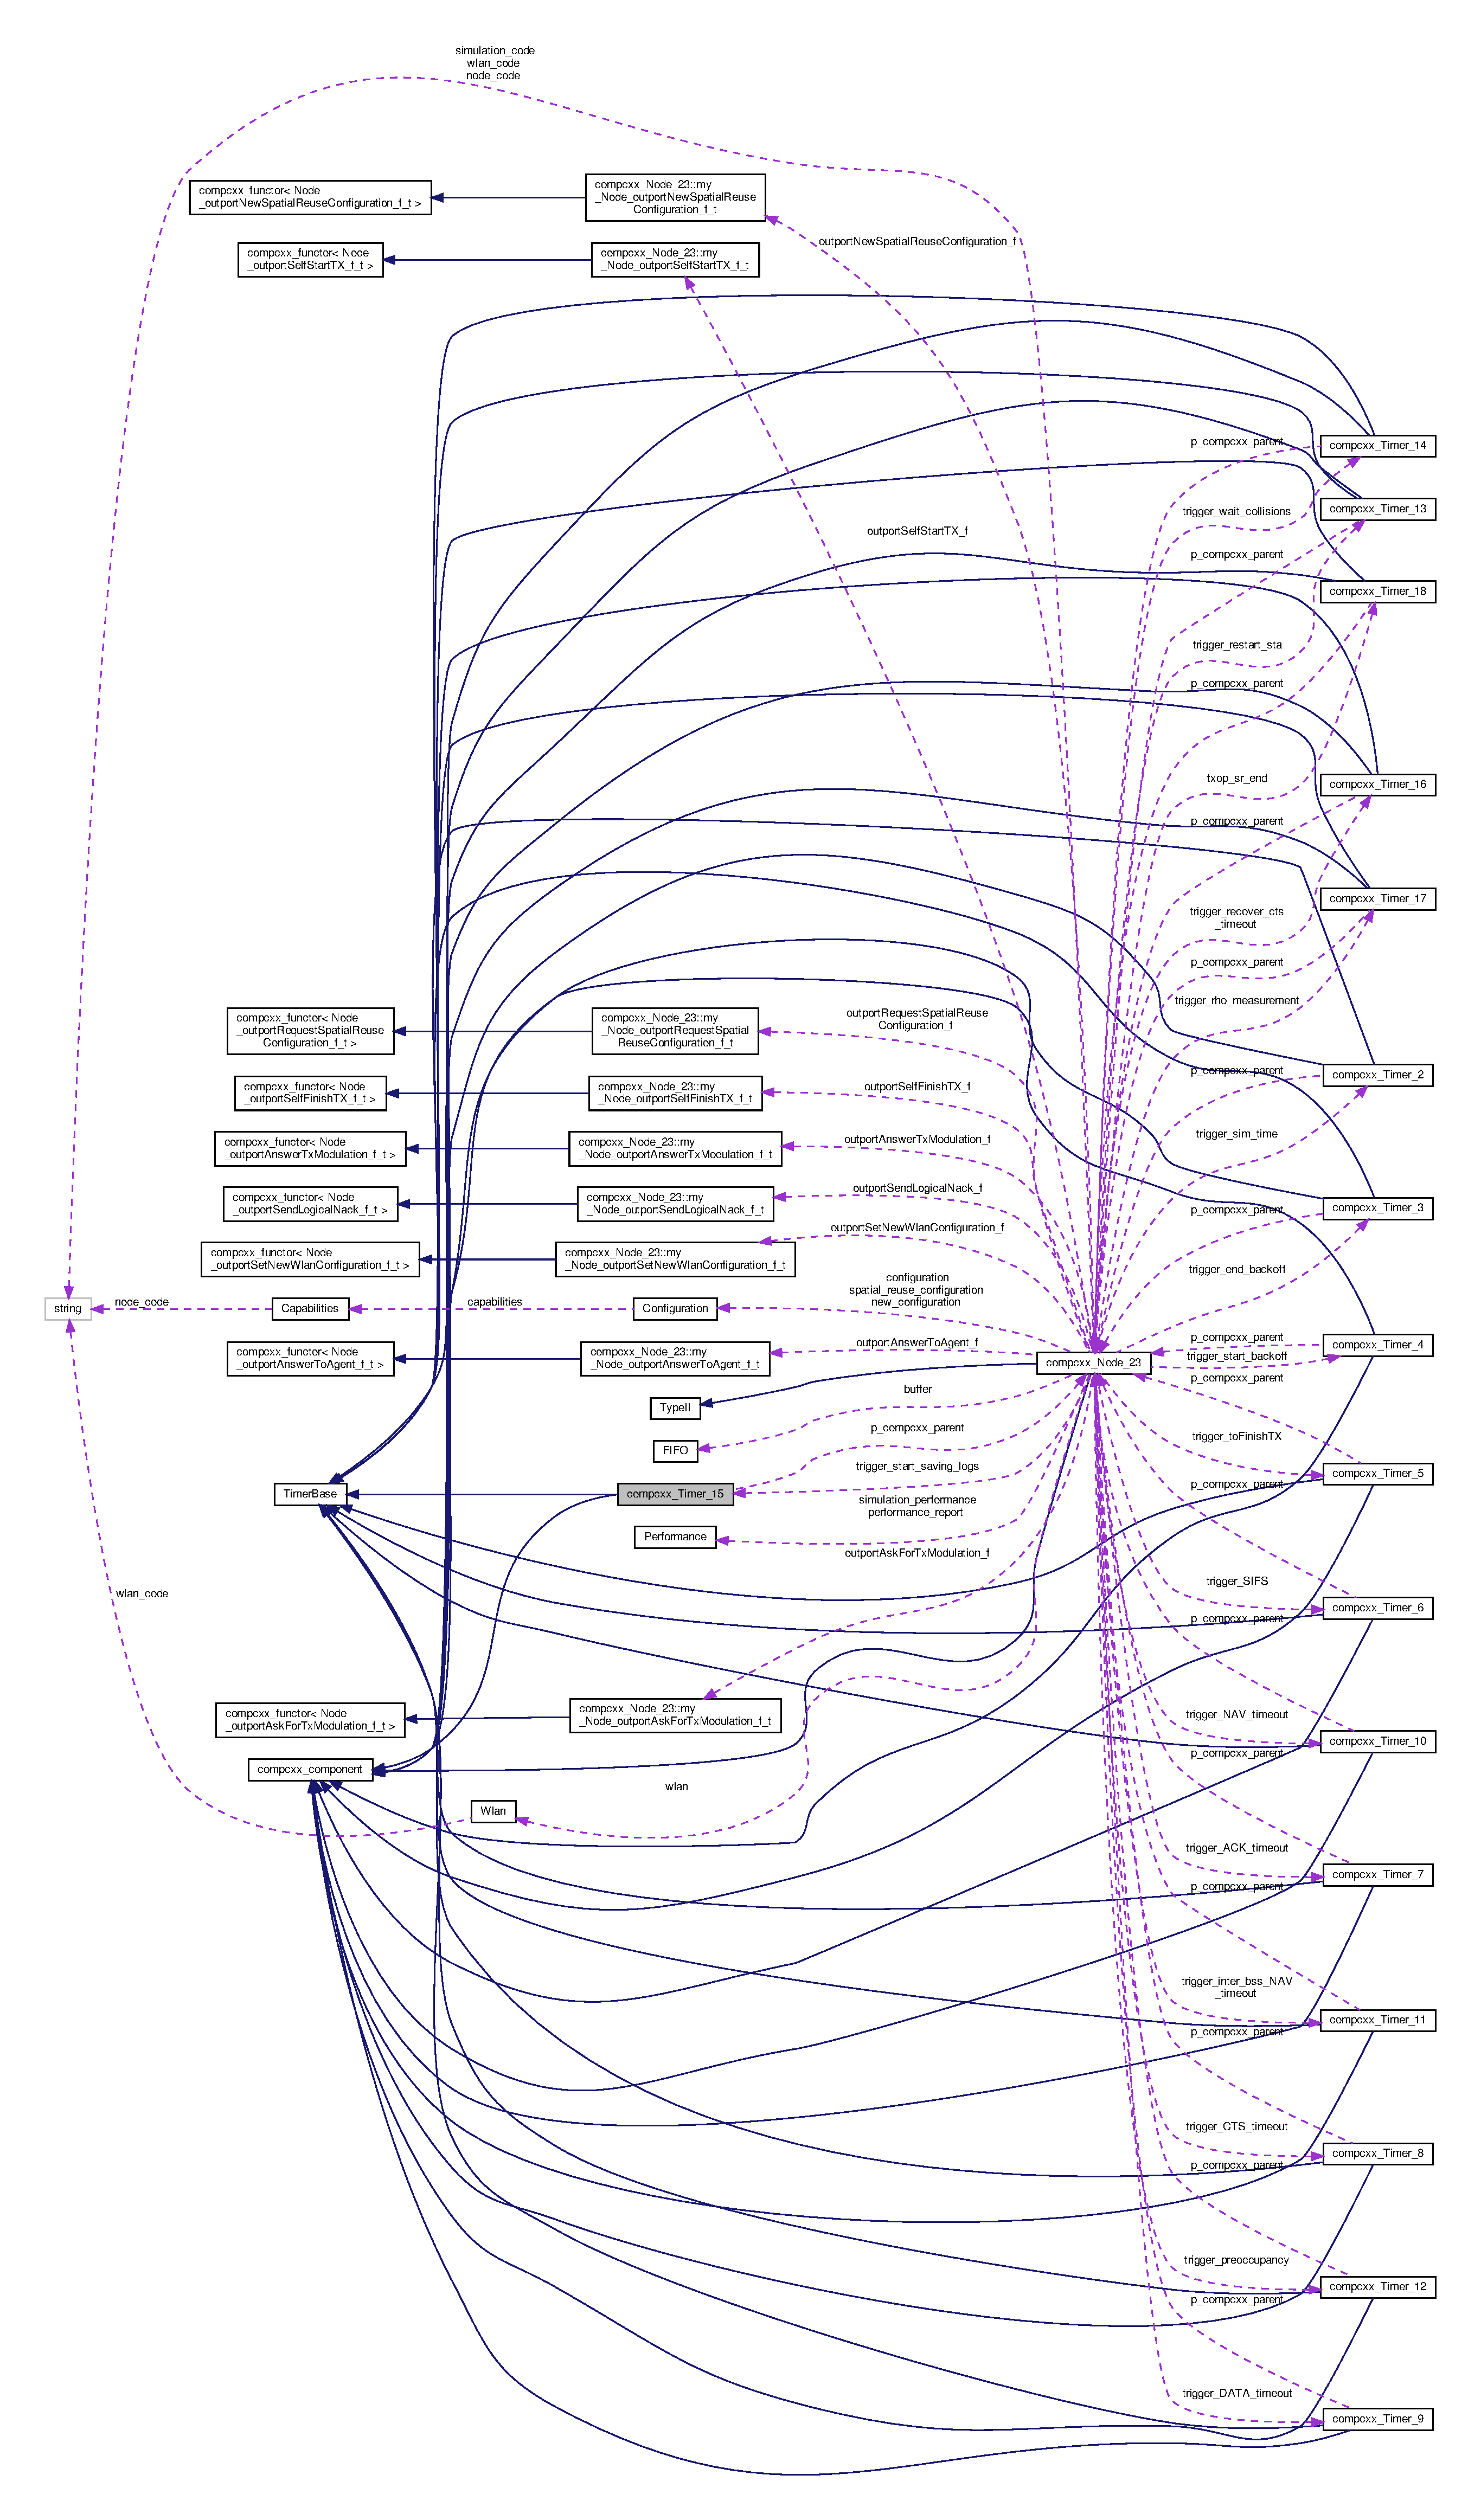
\includegraphics[height=550pt]{classcompcxx__Timer__15__coll__graph}
\end{center}
\end{figure}
\subsection*{Classes}
\begin{DoxyCompactItemize}
\item 
struct \hyperlink{structcompcxx__Timer__15_1_1event__t}{event\+\_\+t}
\end{DoxyCompactItemize}
\subsection*{Public Member Functions}
\begin{DoxyCompactItemize}
\item 
\mbox{\Hypertarget{classcompcxx__Timer__15_aca31ab9ddd664b8bb6171844dd237c0c}\label{classcompcxx__Timer__15_aca31ab9ddd664b8bb6171844dd237c0c}} 
void {\bfseries Set} (\hyperlink{classtrigger__t}{trigger\+\_\+t} const \&, double)
\item 
\mbox{\Hypertarget{classcompcxx__Timer__15_ad3b874ca9f45b7ead1f78709b195b4b5}\label{classcompcxx__Timer__15_ad3b874ca9f45b7ead1f78709b195b4b5}} 
void {\bfseries Set} (double)
\item 
\mbox{\Hypertarget{classcompcxx__Timer__15_a4500c5b451dcb3804cead249557a6773}\label{classcompcxx__Timer__15_a4500c5b451dcb3804cead249557a6773}} 
double {\bfseries Get\+Time} ()
\item 
\mbox{\Hypertarget{classcompcxx__Timer__15_ab654ed590f09eee0163ae8a7e31cbed8}\label{classcompcxx__Timer__15_ab654ed590f09eee0163ae8a7e31cbed8}} 
bool {\bfseries Active} ()
\item 
\mbox{\Hypertarget{classcompcxx__Timer__15_a2a1d5cf192d8e8175df587869d6a3b56}\label{classcompcxx__Timer__15_a2a1d5cf192d8e8175df587869d6a3b56}} 
\hyperlink{classtrigger__t}{trigger\+\_\+t} \& {\bfseries Get\+Data} ()
\item 
\mbox{\Hypertarget{classcompcxx__Timer__15_a43adfdd6fa2e661aeef8905ff3da410a}\label{classcompcxx__Timer__15_a43adfdd6fa2e661aeef8905ff3da410a}} 
void {\bfseries Set\+Data} (\hyperlink{classtrigger__t}{trigger\+\_\+t} const \&d)
\item 
\mbox{\Hypertarget{classcompcxx__Timer__15_a9c7bef59134d87d3e52b549202c8c191}\label{classcompcxx__Timer__15_a9c7bef59134d87d3e52b549202c8c191}} 
void {\bfseries Cancel} ()
\item 
\mbox{\Hypertarget{classcompcxx__Timer__15_a96df3802e1c766e643121db183d0916c}\label{classcompcxx__Timer__15_a96df3802e1c766e643121db183d0916c}} 
void {\bfseries activate} (\hyperlink{structCostEvent}{Cost\+Event} $\ast$)
\end{DoxyCompactItemize}
\subsection*{Public Attributes}
\begin{DoxyCompactItemize}
\item 
\mbox{\Hypertarget{classcompcxx__Timer__15_a027bb3310c79564e74fd9b2956b91148}\label{classcompcxx__Timer__15_a027bb3310c79564e74fd9b2956b91148}} 
\hyperlink{classcompcxx__Node__23}{compcxx\+\_\+\+Node\+\_\+23} $\ast$ {\bfseries p\+\_\+compcxx\+\_\+parent}
\end{DoxyCompactItemize}
\subsection*{Additional Inherited Members}


The documentation for this class was generated from the following file\+:\begin{DoxyCompactItemize}
\item 
Code/main/komondor\+\_\+main.\+cxx\end{DoxyCompactItemize}

\hypertarget{classcompcxx__Timer__16}{}\section{compcxx\+\_\+\+Timer\+\_\+16 Class Reference}
\label{classcompcxx__Timer__16}\index{compcxx\+\_\+\+Timer\+\_\+16@{compcxx\+\_\+\+Timer\+\_\+16}}


Inheritance diagram for compcxx\+\_\+\+Timer\+\_\+16\+:\nopagebreak
\begin{figure}[H]
\begin{center}
\leavevmode
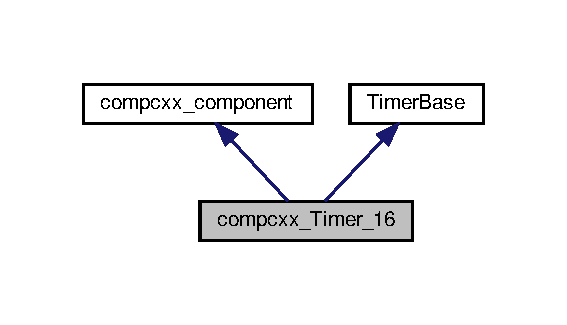
\includegraphics[width=272pt]{classcompcxx__Timer__16__inherit__graph}
\end{center}
\end{figure}


Collaboration diagram for compcxx\+\_\+\+Timer\+\_\+16\+:\nopagebreak
\begin{figure}[H]
\begin{center}
\leavevmode
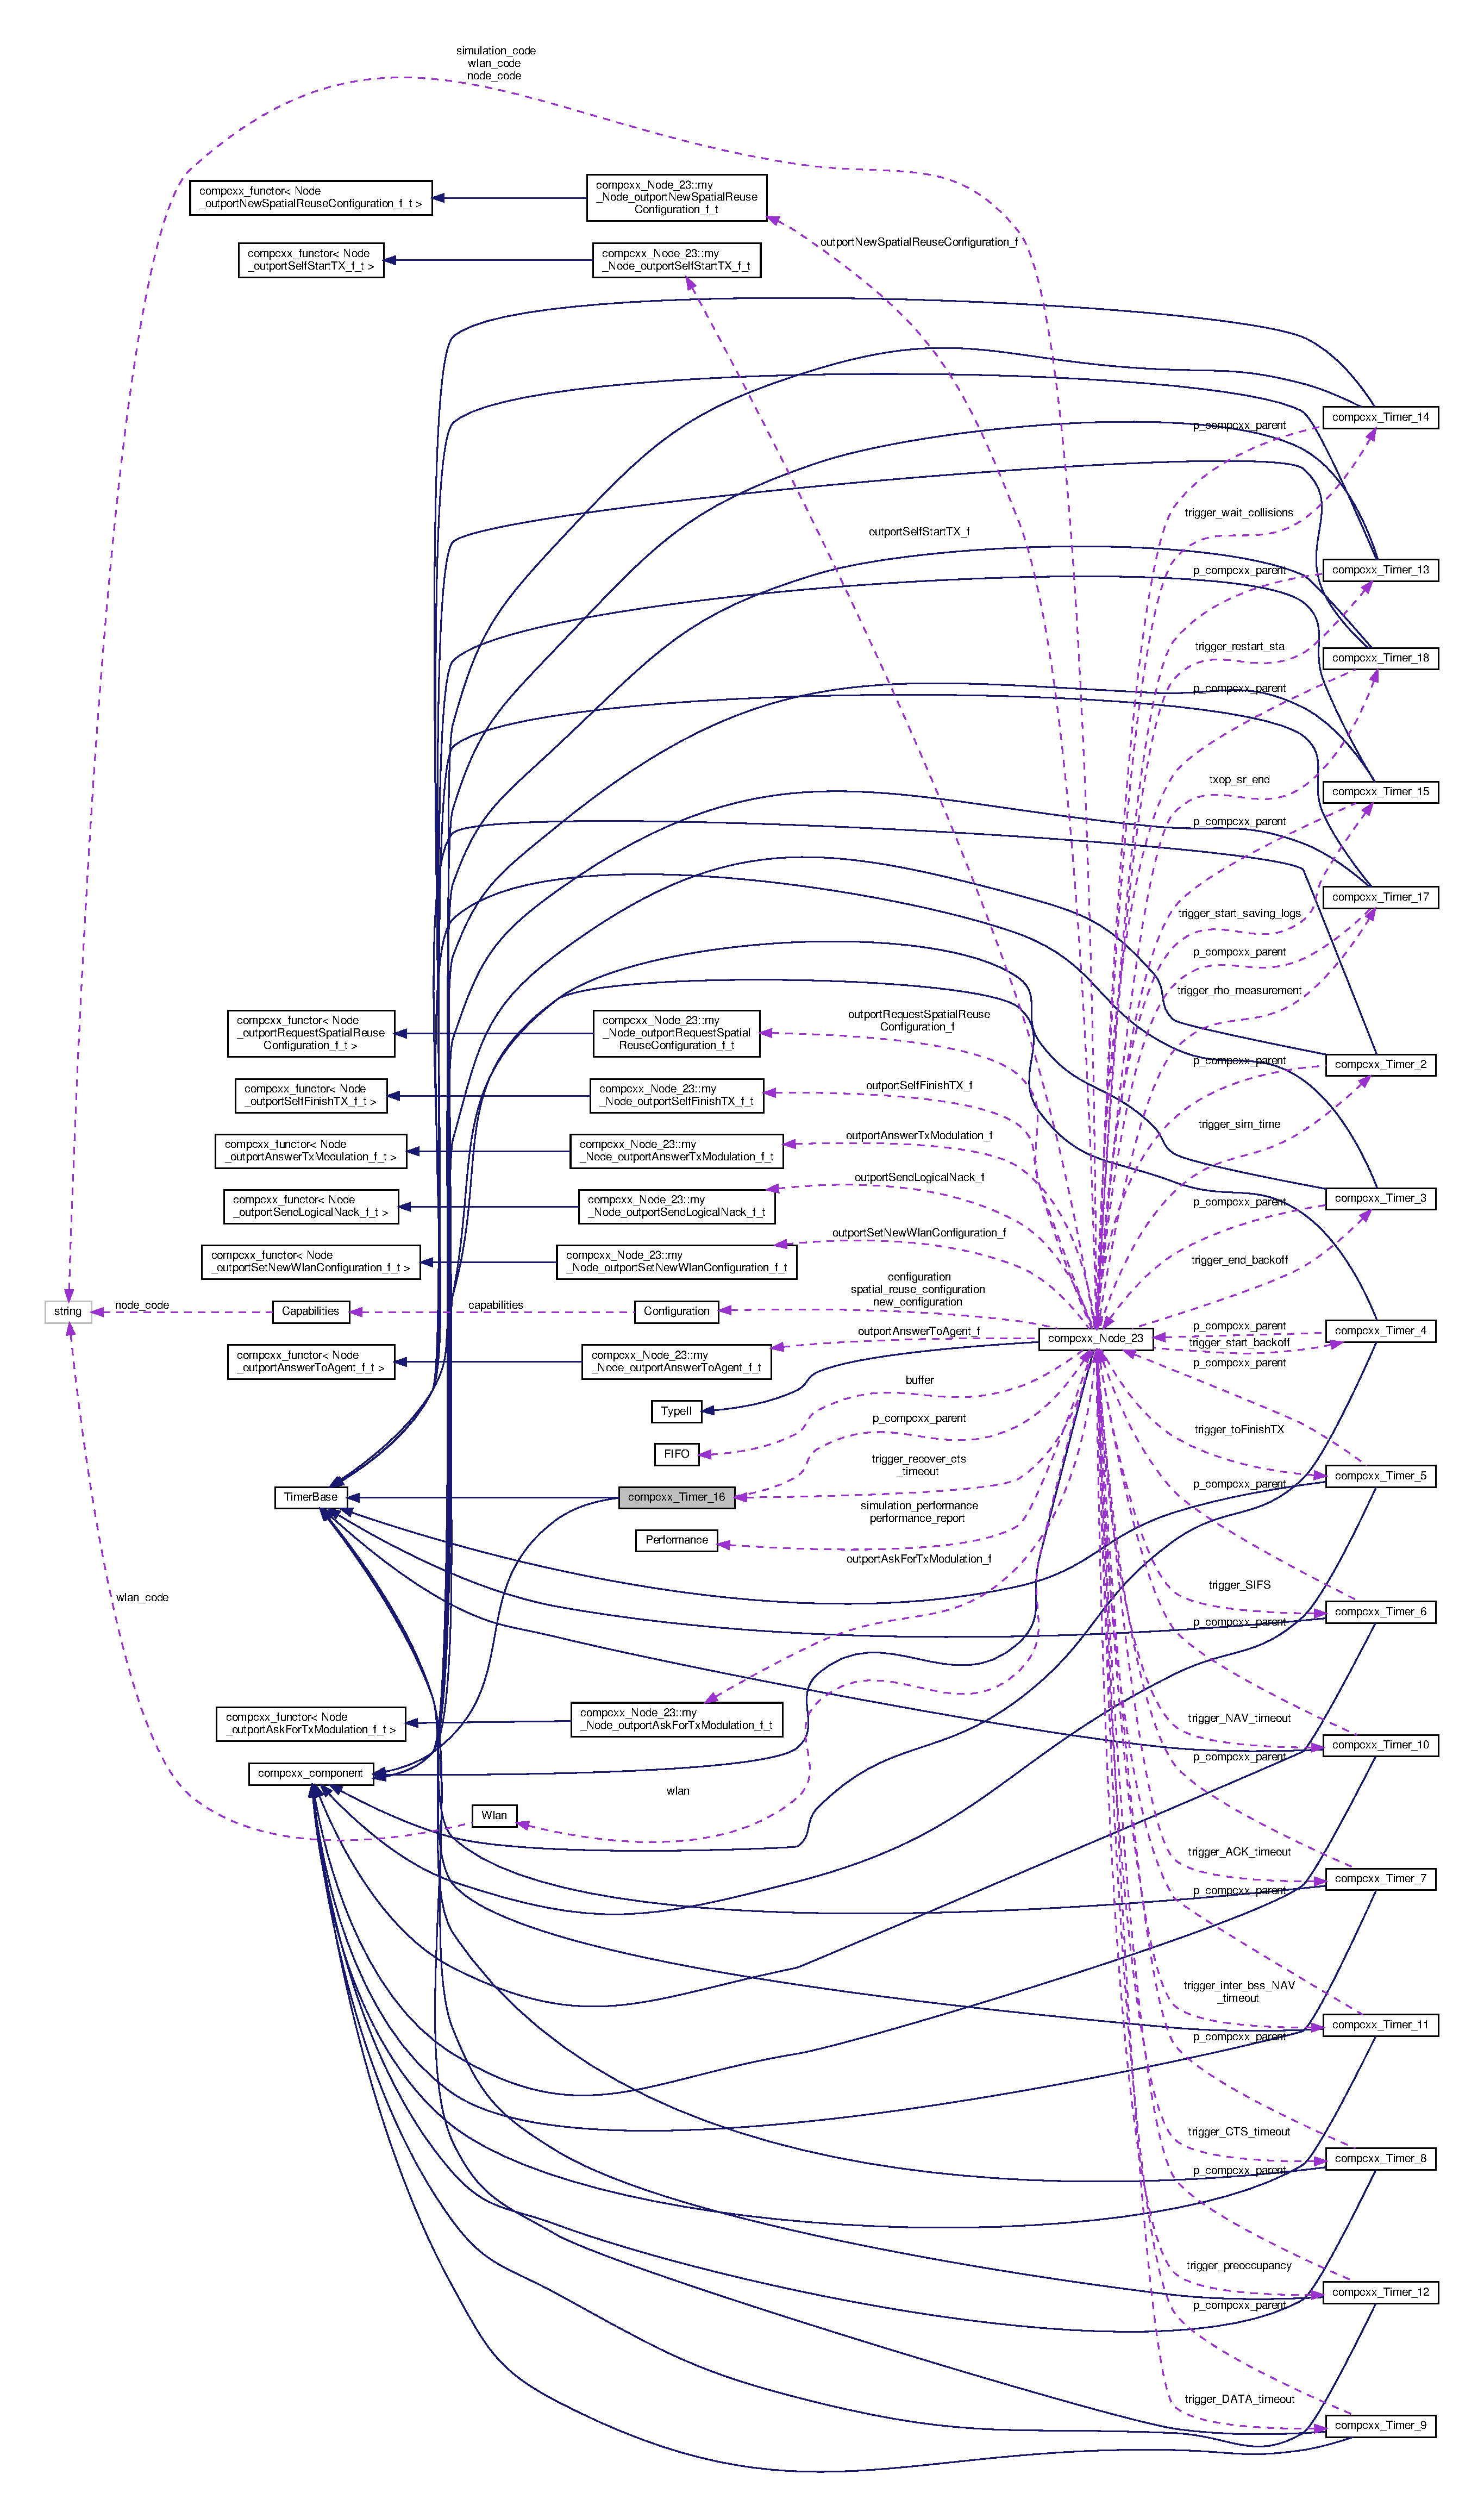
\includegraphics[height=550pt]{classcompcxx__Timer__16__coll__graph}
\end{center}
\end{figure}
\subsection*{Classes}
\begin{DoxyCompactItemize}
\item 
struct \hyperlink{structcompcxx__Timer__16_1_1event__t}{event\+\_\+t}
\end{DoxyCompactItemize}
\subsection*{Public Member Functions}
\begin{DoxyCompactItemize}
\item 
\mbox{\Hypertarget{classcompcxx__Timer__16_aef2336ab7f1871aee203849c70094218}\label{classcompcxx__Timer__16_aef2336ab7f1871aee203849c70094218}} 
void {\bfseries Set} (\hyperlink{classtrigger__t}{trigger\+\_\+t} const \&, double)
\item 
\mbox{\Hypertarget{classcompcxx__Timer__16_ac18467a57608083bd3a7f5df863cf90a}\label{classcompcxx__Timer__16_ac18467a57608083bd3a7f5df863cf90a}} 
void {\bfseries Set} (double)
\item 
\mbox{\Hypertarget{classcompcxx__Timer__16_a57b1be539d2f272a7487ae9ea505fb81}\label{classcompcxx__Timer__16_a57b1be539d2f272a7487ae9ea505fb81}} 
double {\bfseries Get\+Time} ()
\item 
\mbox{\Hypertarget{classcompcxx__Timer__16_ac7219a7d1c00e050b729e749526bdf88}\label{classcompcxx__Timer__16_ac7219a7d1c00e050b729e749526bdf88}} 
bool {\bfseries Active} ()
\item 
\mbox{\Hypertarget{classcompcxx__Timer__16_a4cbf6defd386af8ef40ea2a733921950}\label{classcompcxx__Timer__16_a4cbf6defd386af8ef40ea2a733921950}} 
\hyperlink{classtrigger__t}{trigger\+\_\+t} \& {\bfseries Get\+Data} ()
\item 
\mbox{\Hypertarget{classcompcxx__Timer__16_ab956248699c35ab65565ec279502f8bc}\label{classcompcxx__Timer__16_ab956248699c35ab65565ec279502f8bc}} 
void {\bfseries Set\+Data} (\hyperlink{classtrigger__t}{trigger\+\_\+t} const \&d)
\item 
\mbox{\Hypertarget{classcompcxx__Timer__16_af13c42b9e77a6d6a636efd90f05c9a32}\label{classcompcxx__Timer__16_af13c42b9e77a6d6a636efd90f05c9a32}} 
void {\bfseries Cancel} ()
\item 
\mbox{\Hypertarget{classcompcxx__Timer__16_ad5ed3c4c3793c7f18d1d1fbbccd8ff48}\label{classcompcxx__Timer__16_ad5ed3c4c3793c7f18d1d1fbbccd8ff48}} 
void {\bfseries activate} (\hyperlink{structCostEvent}{Cost\+Event} $\ast$)
\end{DoxyCompactItemize}
\subsection*{Public Attributes}
\begin{DoxyCompactItemize}
\item 
\mbox{\Hypertarget{classcompcxx__Timer__16_acb2d661c8cc5b30c64fdab86db05b5ac}\label{classcompcxx__Timer__16_acb2d661c8cc5b30c64fdab86db05b5ac}} 
\hyperlink{classcompcxx__Node__23}{compcxx\+\_\+\+Node\+\_\+23} $\ast$ {\bfseries p\+\_\+compcxx\+\_\+parent}
\end{DoxyCompactItemize}
\subsection*{Additional Inherited Members}


The documentation for this class was generated from the following file\+:\begin{DoxyCompactItemize}
\item 
Code/main/komondor\+\_\+main.\+cxx\end{DoxyCompactItemize}

\hypertarget{classcompcxx__Timer__17}{}\section{compcxx\+\_\+\+Timer\+\_\+17 Class Reference}
\label{classcompcxx__Timer__17}\index{compcxx\+\_\+\+Timer\+\_\+17@{compcxx\+\_\+\+Timer\+\_\+17}}


Inheritance diagram for compcxx\+\_\+\+Timer\+\_\+17\+:\nopagebreak
\begin{figure}[H]
\begin{center}
\leavevmode
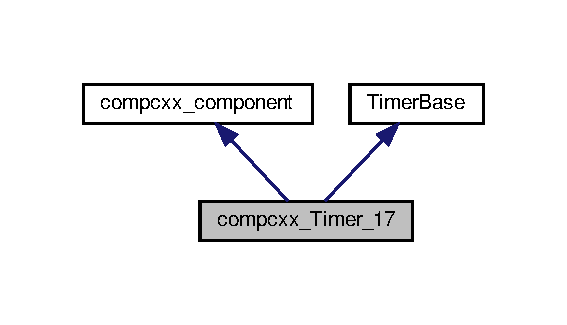
\includegraphics[width=272pt]{classcompcxx__Timer__17__inherit__graph}
\end{center}
\end{figure}


Collaboration diagram for compcxx\+\_\+\+Timer\+\_\+17\+:\nopagebreak
\begin{figure}[H]
\begin{center}
\leavevmode
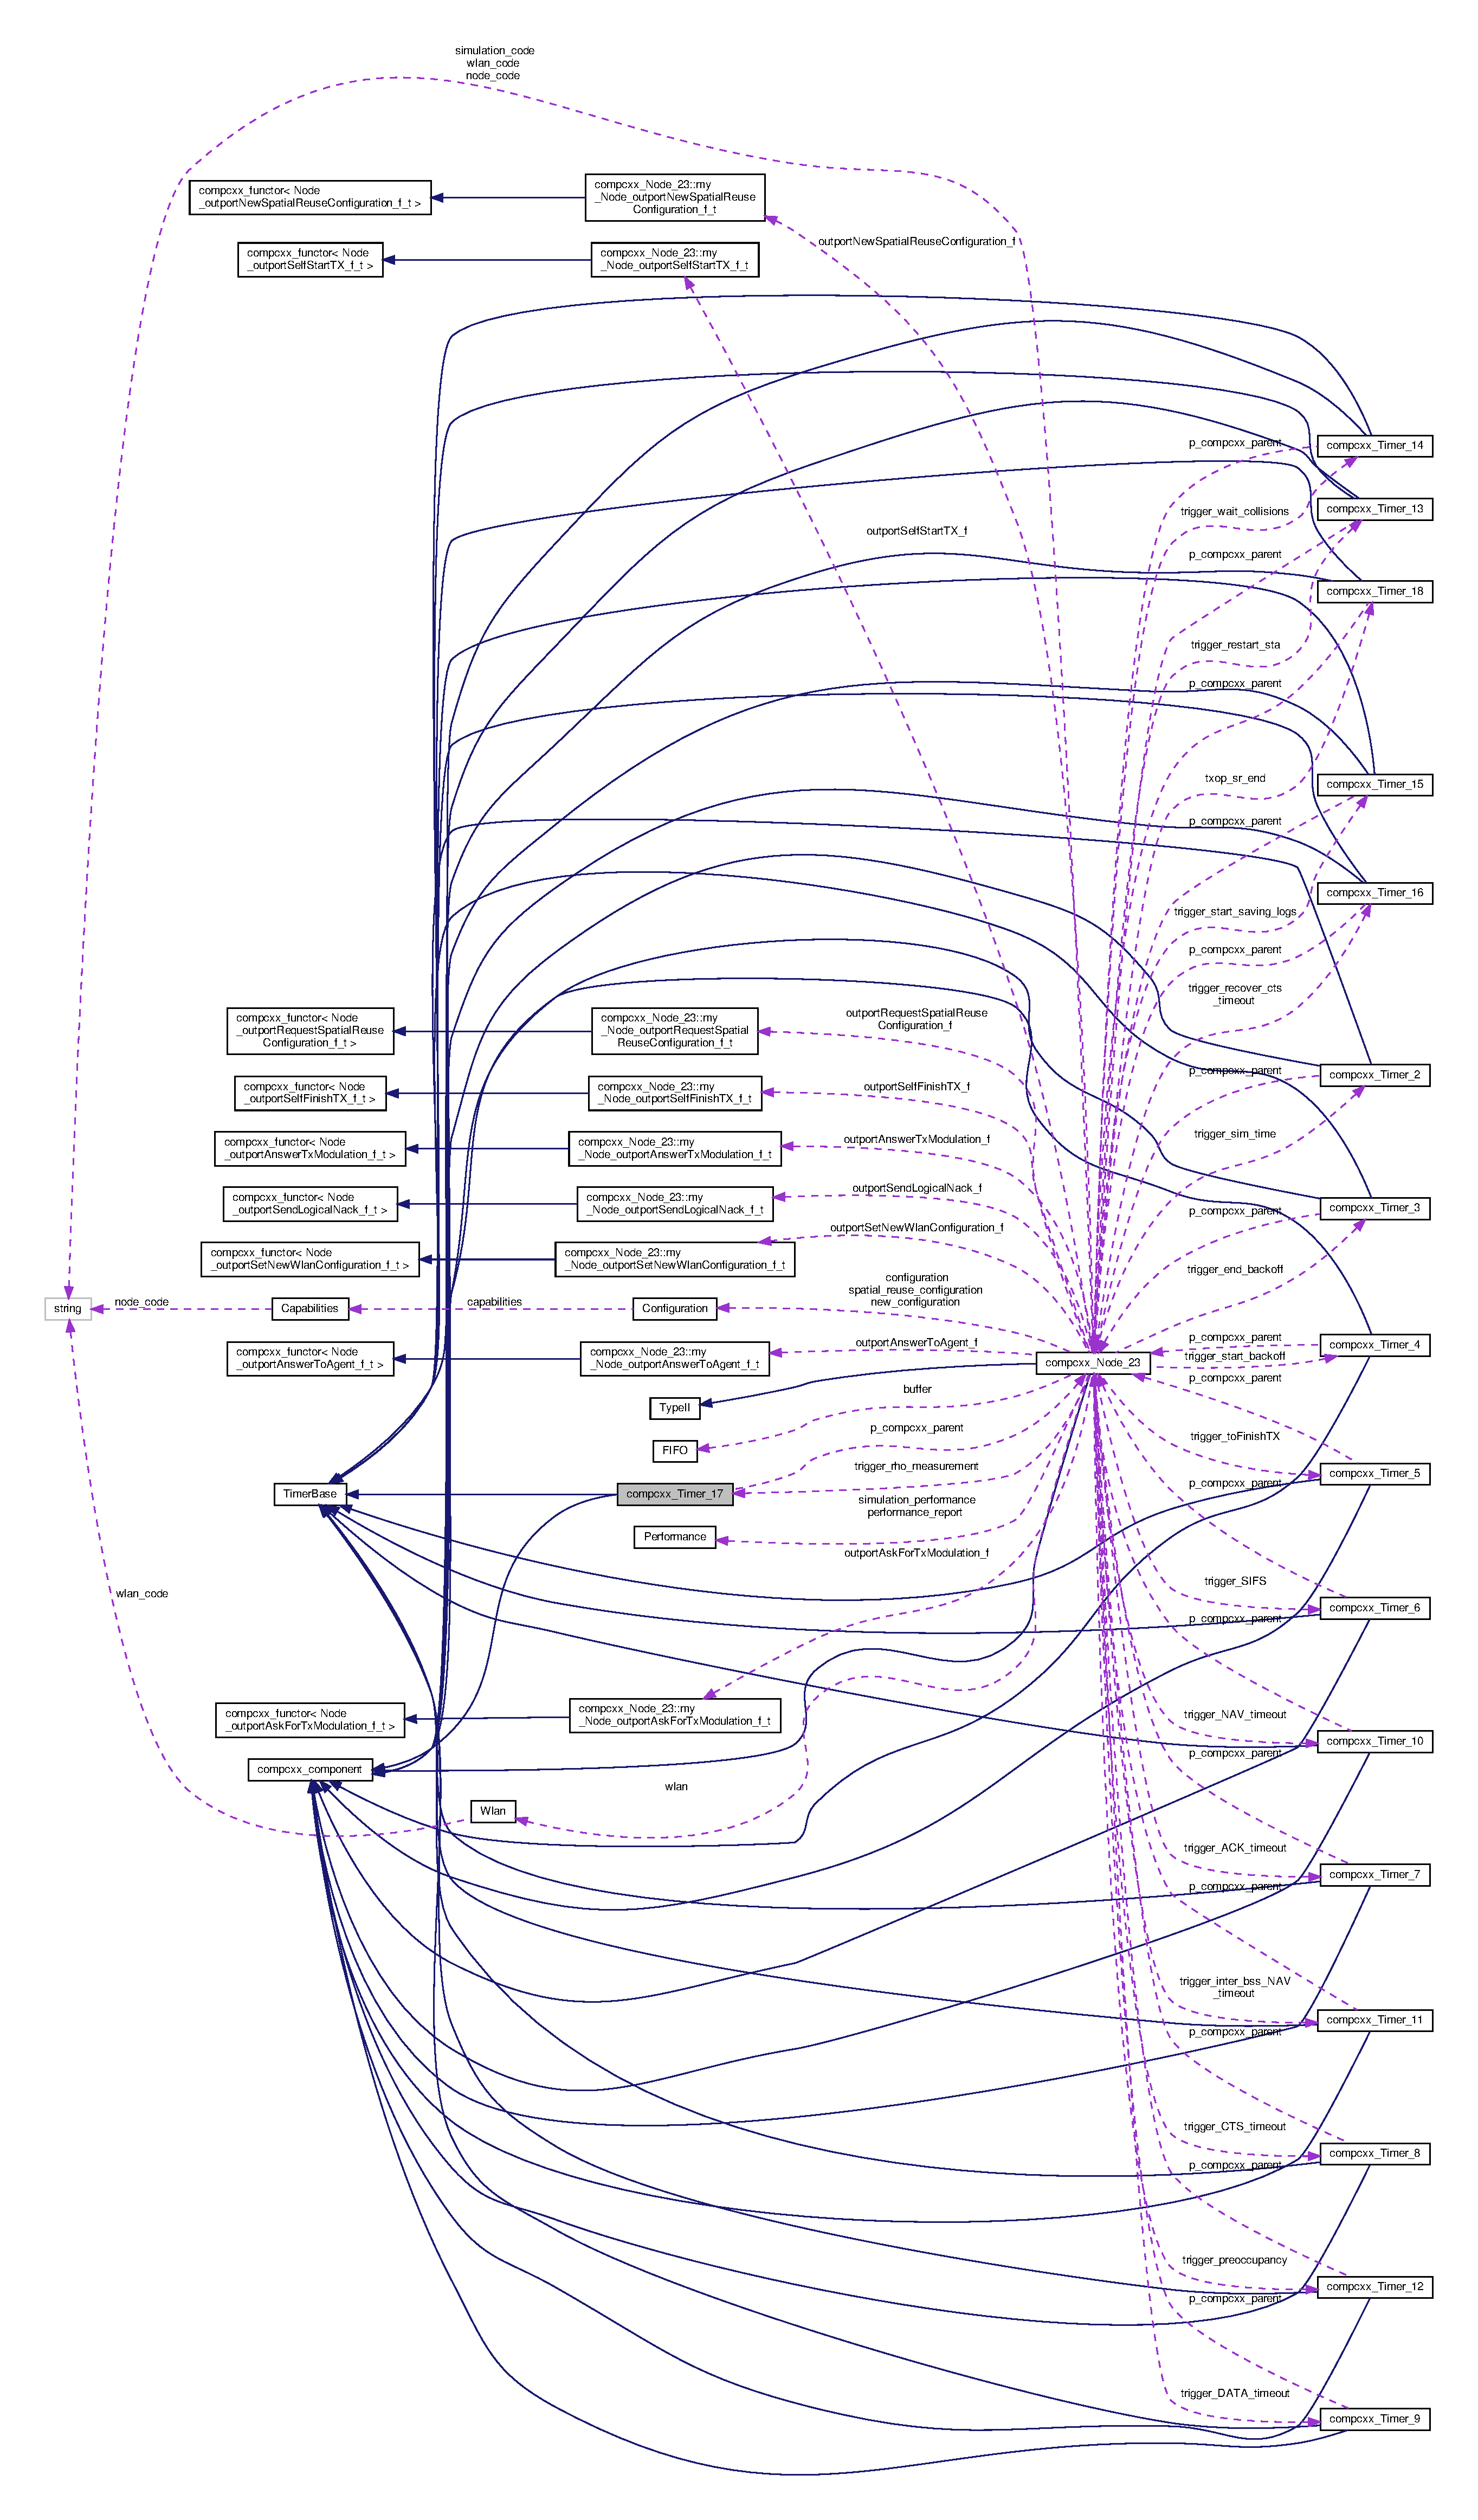
\includegraphics[height=550pt]{classcompcxx__Timer__17__coll__graph}
\end{center}
\end{figure}
\subsection*{Classes}
\begin{DoxyCompactItemize}
\item 
struct \hyperlink{structcompcxx__Timer__17_1_1event__t}{event\+\_\+t}
\end{DoxyCompactItemize}
\subsection*{Public Member Functions}
\begin{DoxyCompactItemize}
\item 
\mbox{\Hypertarget{classcompcxx__Timer__17_a35826e484c0602c6cb1c1cab8522cbaf}\label{classcompcxx__Timer__17_a35826e484c0602c6cb1c1cab8522cbaf}} 
void {\bfseries Set} (\hyperlink{classtrigger__t}{trigger\+\_\+t} const \&, double)
\item 
\mbox{\Hypertarget{classcompcxx__Timer__17_ab03f73490392c5a171008fd4721dda7d}\label{classcompcxx__Timer__17_ab03f73490392c5a171008fd4721dda7d}} 
void {\bfseries Set} (double)
\item 
\mbox{\Hypertarget{classcompcxx__Timer__17_a85ee556f157a1628cd026115b9a928c4}\label{classcompcxx__Timer__17_a85ee556f157a1628cd026115b9a928c4}} 
double {\bfseries Get\+Time} ()
\item 
\mbox{\Hypertarget{classcompcxx__Timer__17_a505106e97d3439297763aa486f21231d}\label{classcompcxx__Timer__17_a505106e97d3439297763aa486f21231d}} 
bool {\bfseries Active} ()
\item 
\mbox{\Hypertarget{classcompcxx__Timer__17_ae202a01a6be8d583e2a66dbfc18c5060}\label{classcompcxx__Timer__17_ae202a01a6be8d583e2a66dbfc18c5060}} 
\hyperlink{classtrigger__t}{trigger\+\_\+t} \& {\bfseries Get\+Data} ()
\item 
\mbox{\Hypertarget{classcompcxx__Timer__17_a7d46ab74fd84c65e9311ca502602683b}\label{classcompcxx__Timer__17_a7d46ab74fd84c65e9311ca502602683b}} 
void {\bfseries Set\+Data} (\hyperlink{classtrigger__t}{trigger\+\_\+t} const \&d)
\item 
\mbox{\Hypertarget{classcompcxx__Timer__17_a9fd63a8cde4df4d4145b004e8f790e70}\label{classcompcxx__Timer__17_a9fd63a8cde4df4d4145b004e8f790e70}} 
void {\bfseries Cancel} ()
\item 
\mbox{\Hypertarget{classcompcxx__Timer__17_af34e3291738398f0a652a763abc54350}\label{classcompcxx__Timer__17_af34e3291738398f0a652a763abc54350}} 
void {\bfseries activate} (\hyperlink{structCostEvent}{Cost\+Event} $\ast$)
\end{DoxyCompactItemize}
\subsection*{Public Attributes}
\begin{DoxyCompactItemize}
\item 
\mbox{\Hypertarget{classcompcxx__Timer__17_a38e21fca153f0e0bb4a9186ce59403ef}\label{classcompcxx__Timer__17_a38e21fca153f0e0bb4a9186ce59403ef}} 
\hyperlink{classcompcxx__Node__23}{compcxx\+\_\+\+Node\+\_\+23} $\ast$ {\bfseries p\+\_\+compcxx\+\_\+parent}
\end{DoxyCompactItemize}
\subsection*{Additional Inherited Members}


The documentation for this class was generated from the following file\+:\begin{DoxyCompactItemize}
\item 
Code/main/komondor\+\_\+main.\+cxx\end{DoxyCompactItemize}

\hypertarget{classcompcxx__Timer__18}{}\section{compcxx\+\_\+\+Timer\+\_\+18 Class Reference}
\label{classcompcxx__Timer__18}\index{compcxx\+\_\+\+Timer\+\_\+18@{compcxx\+\_\+\+Timer\+\_\+18}}


Inheritance diagram for compcxx\+\_\+\+Timer\+\_\+18\+:\nopagebreak
\begin{figure}[H]
\begin{center}
\leavevmode
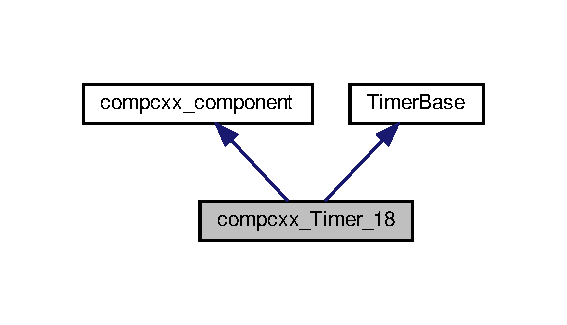
\includegraphics[width=272pt]{classcompcxx__Timer__18__inherit__graph}
\end{center}
\end{figure}


Collaboration diagram for compcxx\+\_\+\+Timer\+\_\+18\+:\nopagebreak
\begin{figure}[H]
\begin{center}
\leavevmode
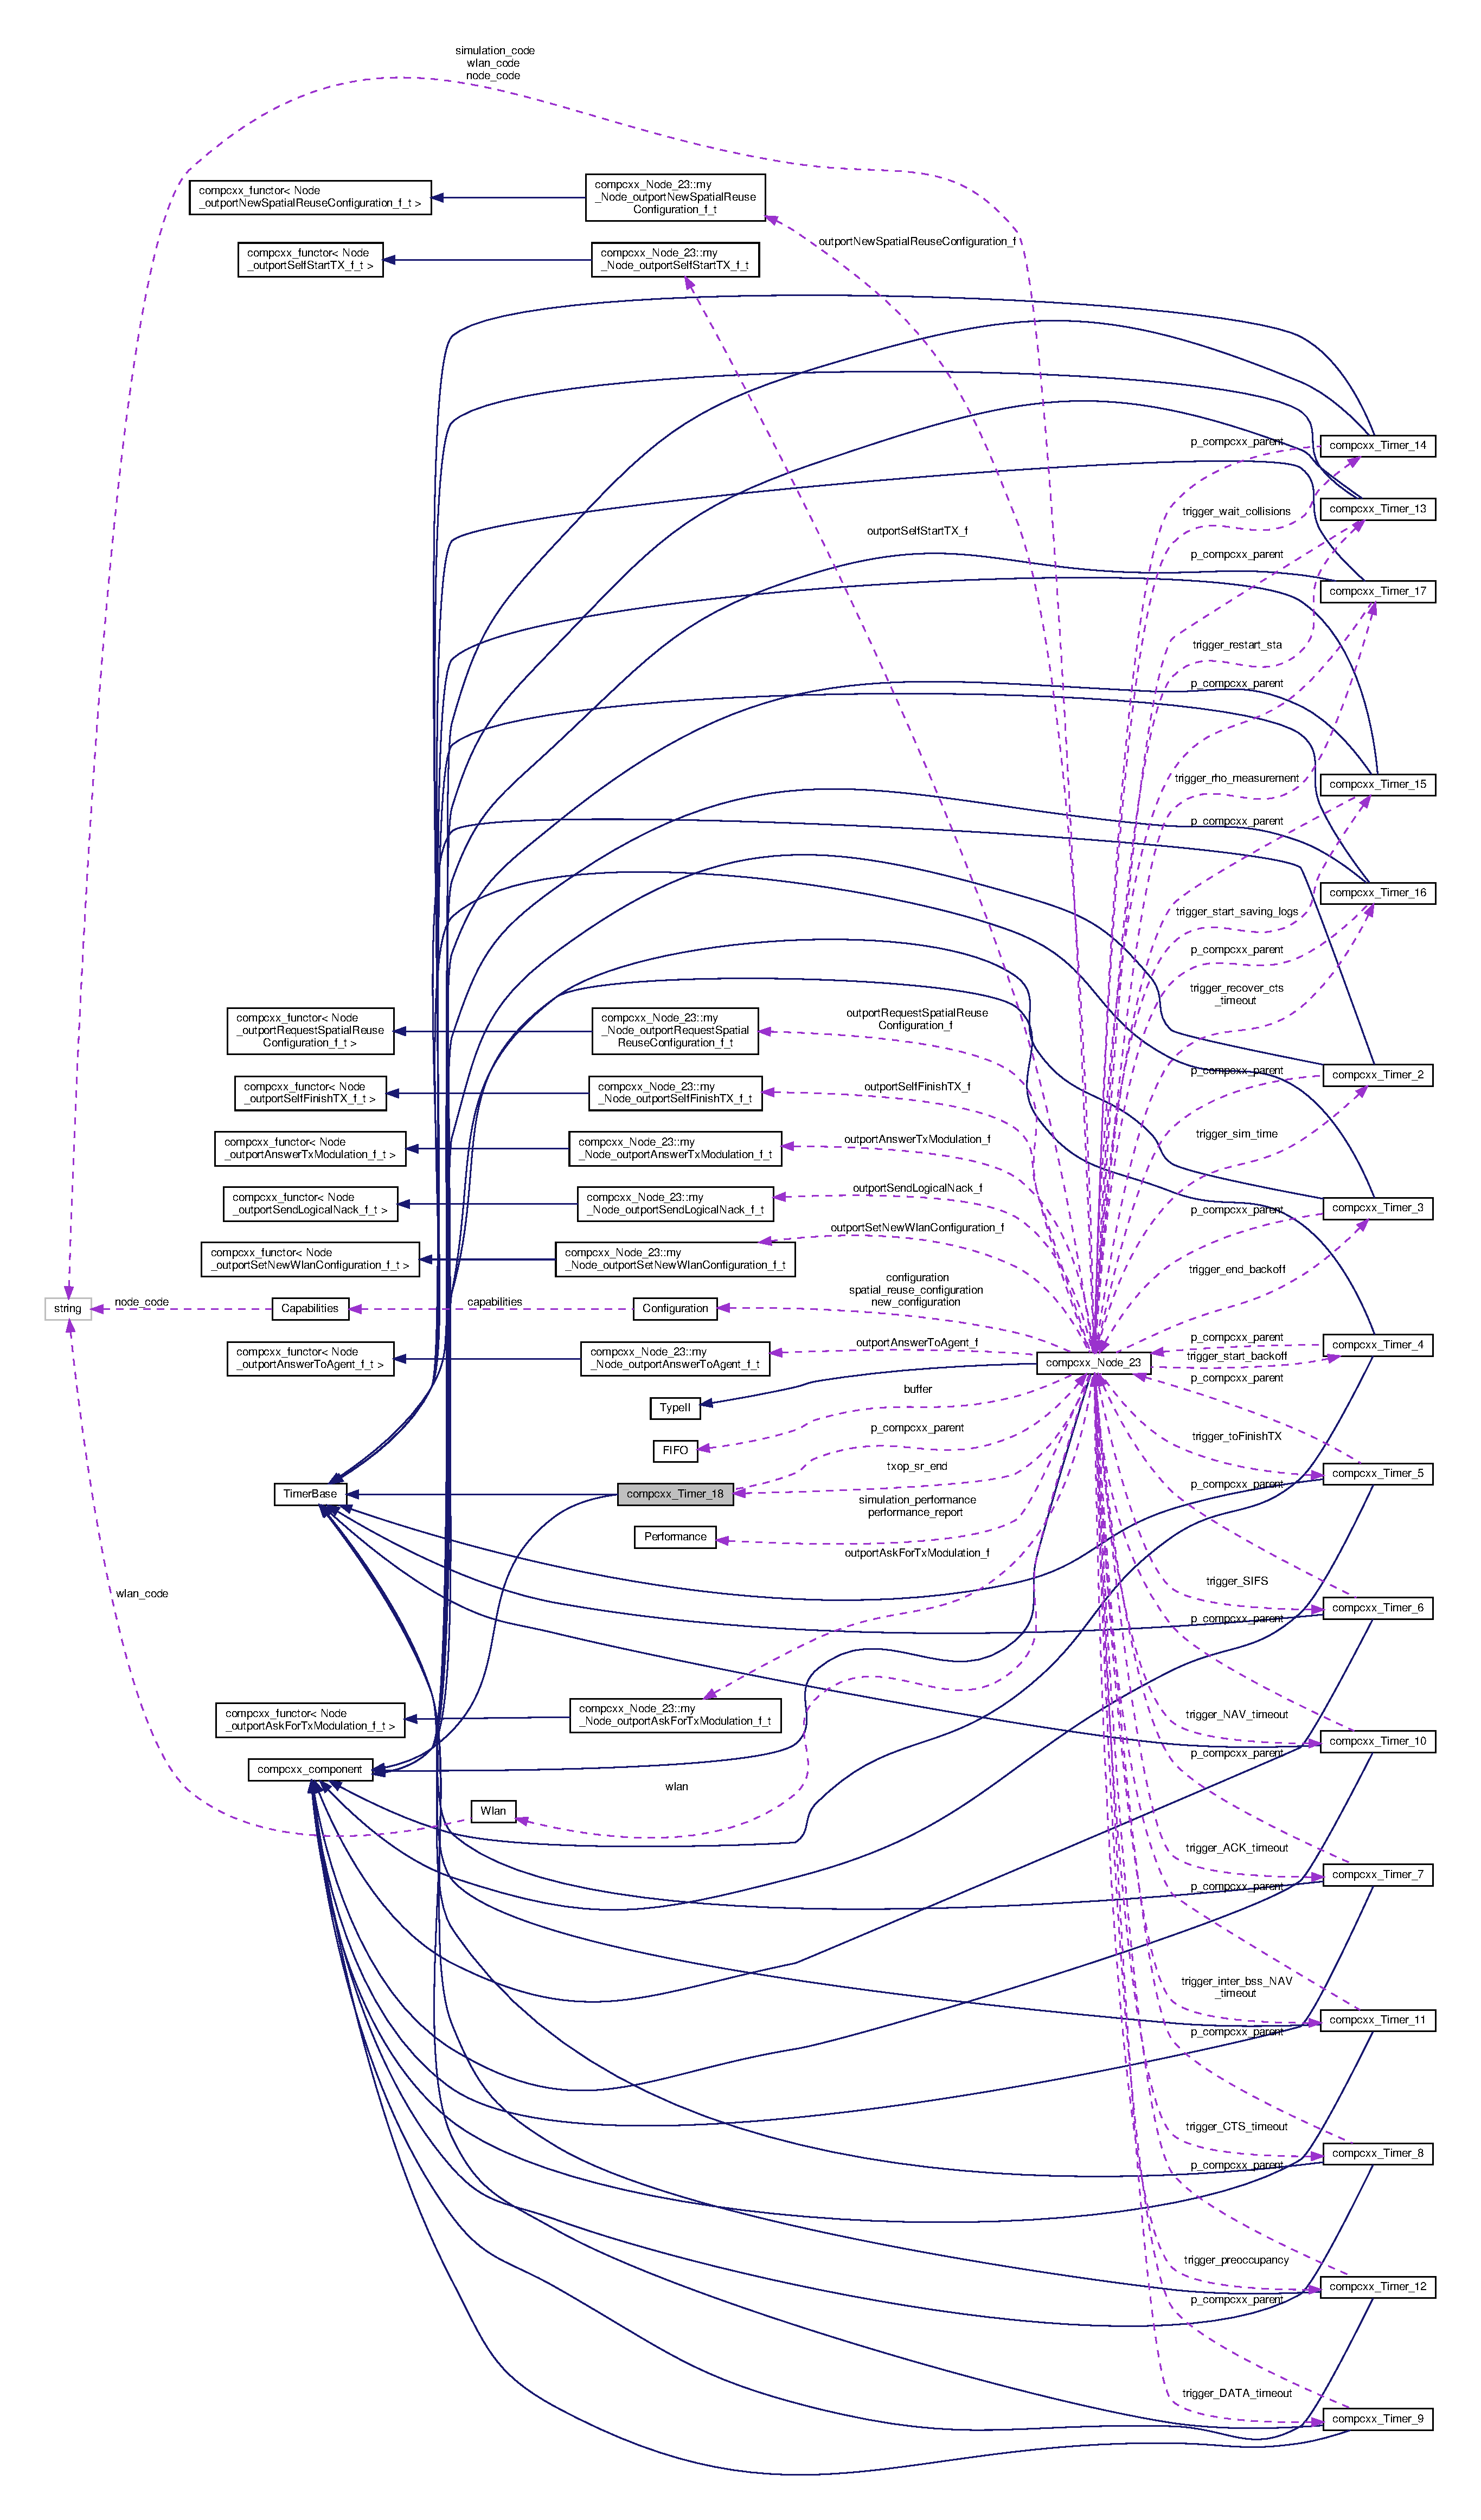
\includegraphics[height=550pt]{classcompcxx__Timer__18__coll__graph}
\end{center}
\end{figure}
\subsection*{Classes}
\begin{DoxyCompactItemize}
\item 
struct \hyperlink{structcompcxx__Timer__18_1_1event__t}{event\+\_\+t}
\end{DoxyCompactItemize}
\subsection*{Public Member Functions}
\begin{DoxyCompactItemize}
\item 
\mbox{\Hypertarget{classcompcxx__Timer__18_a099b384bd2f8f8cd63637de2bfc3d374}\label{classcompcxx__Timer__18_a099b384bd2f8f8cd63637de2bfc3d374}} 
void {\bfseries Set} (\hyperlink{classtrigger__t}{trigger\+\_\+t} const \&, double)
\item 
\mbox{\Hypertarget{classcompcxx__Timer__18_a4ba344391107be36bd60328970785748}\label{classcompcxx__Timer__18_a4ba344391107be36bd60328970785748}} 
void {\bfseries Set} (double)
\item 
\mbox{\Hypertarget{classcompcxx__Timer__18_a90b5faa5f071efe55cfb44cdec5562f5}\label{classcompcxx__Timer__18_a90b5faa5f071efe55cfb44cdec5562f5}} 
double {\bfseries Get\+Time} ()
\item 
\mbox{\Hypertarget{classcompcxx__Timer__18_a3dc0564262fff44a94f4fd639dfb2b26}\label{classcompcxx__Timer__18_a3dc0564262fff44a94f4fd639dfb2b26}} 
bool {\bfseries Active} ()
\item 
\mbox{\Hypertarget{classcompcxx__Timer__18_a92bdf186448eac7ba7e2cb8b13b5dd99}\label{classcompcxx__Timer__18_a92bdf186448eac7ba7e2cb8b13b5dd99}} 
\hyperlink{classtrigger__t}{trigger\+\_\+t} \& {\bfseries Get\+Data} ()
\item 
\mbox{\Hypertarget{classcompcxx__Timer__18_ab617bfbf6debc99962c2eeea3da31d77}\label{classcompcxx__Timer__18_ab617bfbf6debc99962c2eeea3da31d77}} 
void {\bfseries Set\+Data} (\hyperlink{classtrigger__t}{trigger\+\_\+t} const \&d)
\item 
\mbox{\Hypertarget{classcompcxx__Timer__18_a937cec56a40d9c1e269028d733946086}\label{classcompcxx__Timer__18_a937cec56a40d9c1e269028d733946086}} 
void {\bfseries Cancel} ()
\item 
\mbox{\Hypertarget{classcompcxx__Timer__18_a1b941bbbe10e3bf6b25c055d474b960f}\label{classcompcxx__Timer__18_a1b941bbbe10e3bf6b25c055d474b960f}} 
void {\bfseries activate} (\hyperlink{structCostEvent}{Cost\+Event} $\ast$)
\end{DoxyCompactItemize}
\subsection*{Public Attributes}
\begin{DoxyCompactItemize}
\item 
\mbox{\Hypertarget{classcompcxx__Timer__18_a878a9da0c5e50899d81ccef1da95e0b8}\label{classcompcxx__Timer__18_a878a9da0c5e50899d81ccef1da95e0b8}} 
\hyperlink{classcompcxx__Node__23}{compcxx\+\_\+\+Node\+\_\+23} $\ast$ {\bfseries p\+\_\+compcxx\+\_\+parent}
\end{DoxyCompactItemize}
\subsection*{Additional Inherited Members}


The documentation for this class was generated from the following file\+:\begin{DoxyCompactItemize}
\item 
Code/main/komondor\+\_\+main.\+cxx\end{DoxyCompactItemize}

\hypertarget{classcompcxx__Timer__19}{}\section{compcxx\+\_\+\+Timer\+\_\+19 Class Reference}
\label{classcompcxx__Timer__19}\index{compcxx\+\_\+\+Timer\+\_\+19@{compcxx\+\_\+\+Timer\+\_\+19}}


Inheritance diagram for compcxx\+\_\+\+Timer\+\_\+19\+:\nopagebreak
\begin{figure}[H]
\begin{center}
\leavevmode
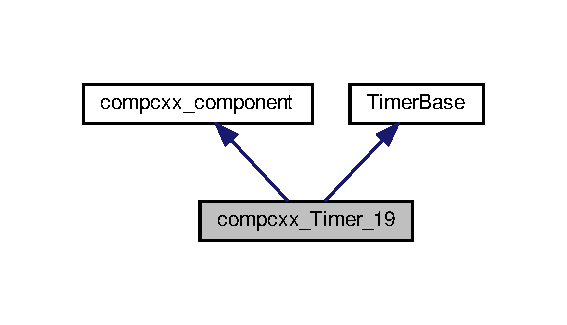
\includegraphics[width=272pt]{classcompcxx__Timer__19__inherit__graph}
\end{center}
\end{figure}


Collaboration diagram for compcxx\+\_\+\+Timer\+\_\+19\+:\nopagebreak
\begin{figure}[H]
\begin{center}
\leavevmode
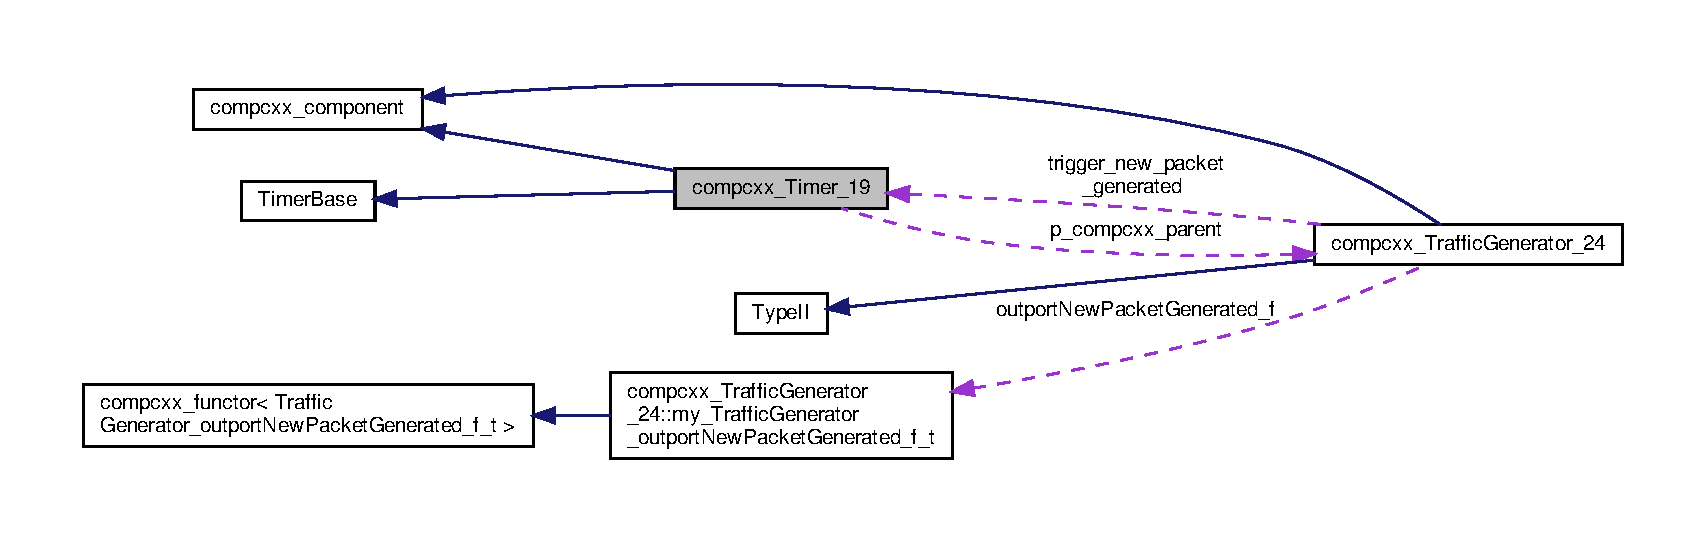
\includegraphics[width=350pt]{classcompcxx__Timer__19__coll__graph}
\end{center}
\end{figure}
\subsection*{Classes}
\begin{DoxyCompactItemize}
\item 
struct \hyperlink{structcompcxx__Timer__19_1_1event__t}{event\+\_\+t}
\end{DoxyCompactItemize}
\subsection*{Public Member Functions}
\begin{DoxyCompactItemize}
\item 
\mbox{\Hypertarget{classcompcxx__Timer__19_a890822acebfe6c41eacbe0e56590fa4b}\label{classcompcxx__Timer__19_a890822acebfe6c41eacbe0e56590fa4b}} 
void {\bfseries Set} (\hyperlink{classtrigger__t}{trigger\+\_\+t} const \&, double)
\item 
\mbox{\Hypertarget{classcompcxx__Timer__19_a57e60e14bb14f7d25a56001492924907}\label{classcompcxx__Timer__19_a57e60e14bb14f7d25a56001492924907}} 
void {\bfseries Set} (double)
\item 
\mbox{\Hypertarget{classcompcxx__Timer__19_adaf3528cf9b3f71483052b1681af7647}\label{classcompcxx__Timer__19_adaf3528cf9b3f71483052b1681af7647}} 
double {\bfseries Get\+Time} ()
\item 
\mbox{\Hypertarget{classcompcxx__Timer__19_ae046f9b3dc0126970a23340a58d7e725}\label{classcompcxx__Timer__19_ae046f9b3dc0126970a23340a58d7e725}} 
bool {\bfseries Active} ()
\item 
\mbox{\Hypertarget{classcompcxx__Timer__19_a2ee4fbceb2884cba8664d3beef83a3c5}\label{classcompcxx__Timer__19_a2ee4fbceb2884cba8664d3beef83a3c5}} 
\hyperlink{classtrigger__t}{trigger\+\_\+t} \& {\bfseries Get\+Data} ()
\item 
\mbox{\Hypertarget{classcompcxx__Timer__19_a683a9c82f0cf1b4816d2c1234fd367b6}\label{classcompcxx__Timer__19_a683a9c82f0cf1b4816d2c1234fd367b6}} 
void {\bfseries Set\+Data} (\hyperlink{classtrigger__t}{trigger\+\_\+t} const \&d)
\item 
\mbox{\Hypertarget{classcompcxx__Timer__19_aac49ad916ffaa0d4ef75249d5a9d9844}\label{classcompcxx__Timer__19_aac49ad916ffaa0d4ef75249d5a9d9844}} 
void {\bfseries Cancel} ()
\item 
\mbox{\Hypertarget{classcompcxx__Timer__19_ad8c35dda9c46490e6f7990e0c3aa4fcf}\label{classcompcxx__Timer__19_ad8c35dda9c46490e6f7990e0c3aa4fcf}} 
void {\bfseries activate} (\hyperlink{structCostEvent}{Cost\+Event} $\ast$)
\end{DoxyCompactItemize}
\subsection*{Public Attributes}
\begin{DoxyCompactItemize}
\item 
\mbox{\Hypertarget{classcompcxx__Timer__19_a132d8e61cfa9450e522c92dcd37e184e}\label{classcompcxx__Timer__19_a132d8e61cfa9450e522c92dcd37e184e}} 
\hyperlink{classcompcxx__TrafficGenerator__24}{compcxx\+\_\+\+Traffic\+Generator\+\_\+24} $\ast$ {\bfseries p\+\_\+compcxx\+\_\+parent}
\end{DoxyCompactItemize}
\subsection*{Additional Inherited Members}


The documentation for this class was generated from the following file\+:\begin{DoxyCompactItemize}
\item 
Code/main/komondor\+\_\+main.\+cxx\end{DoxyCompactItemize}

\hypertarget{classcompcxx__Timer__2}{}\section{compcxx\+\_\+\+Timer\+\_\+2 Class Reference}
\label{classcompcxx__Timer__2}\index{compcxx\+\_\+\+Timer\+\_\+2@{compcxx\+\_\+\+Timer\+\_\+2}}


Inheritance diagram for compcxx\+\_\+\+Timer\+\_\+2\+:\nopagebreak
\begin{figure}[H]
\begin{center}
\leavevmode
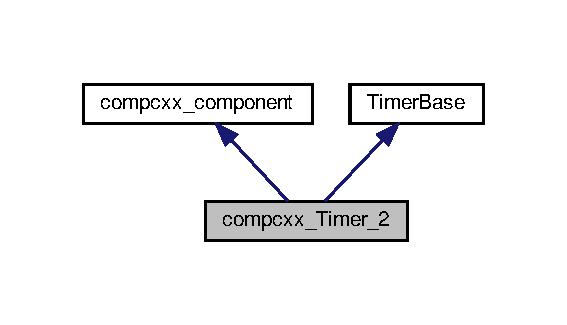
\includegraphics[width=272pt]{classcompcxx__Timer__2__inherit__graph}
\end{center}
\end{figure}


Collaboration diagram for compcxx\+\_\+\+Timer\+\_\+2\+:\nopagebreak
\begin{figure}[H]
\begin{center}
\leavevmode
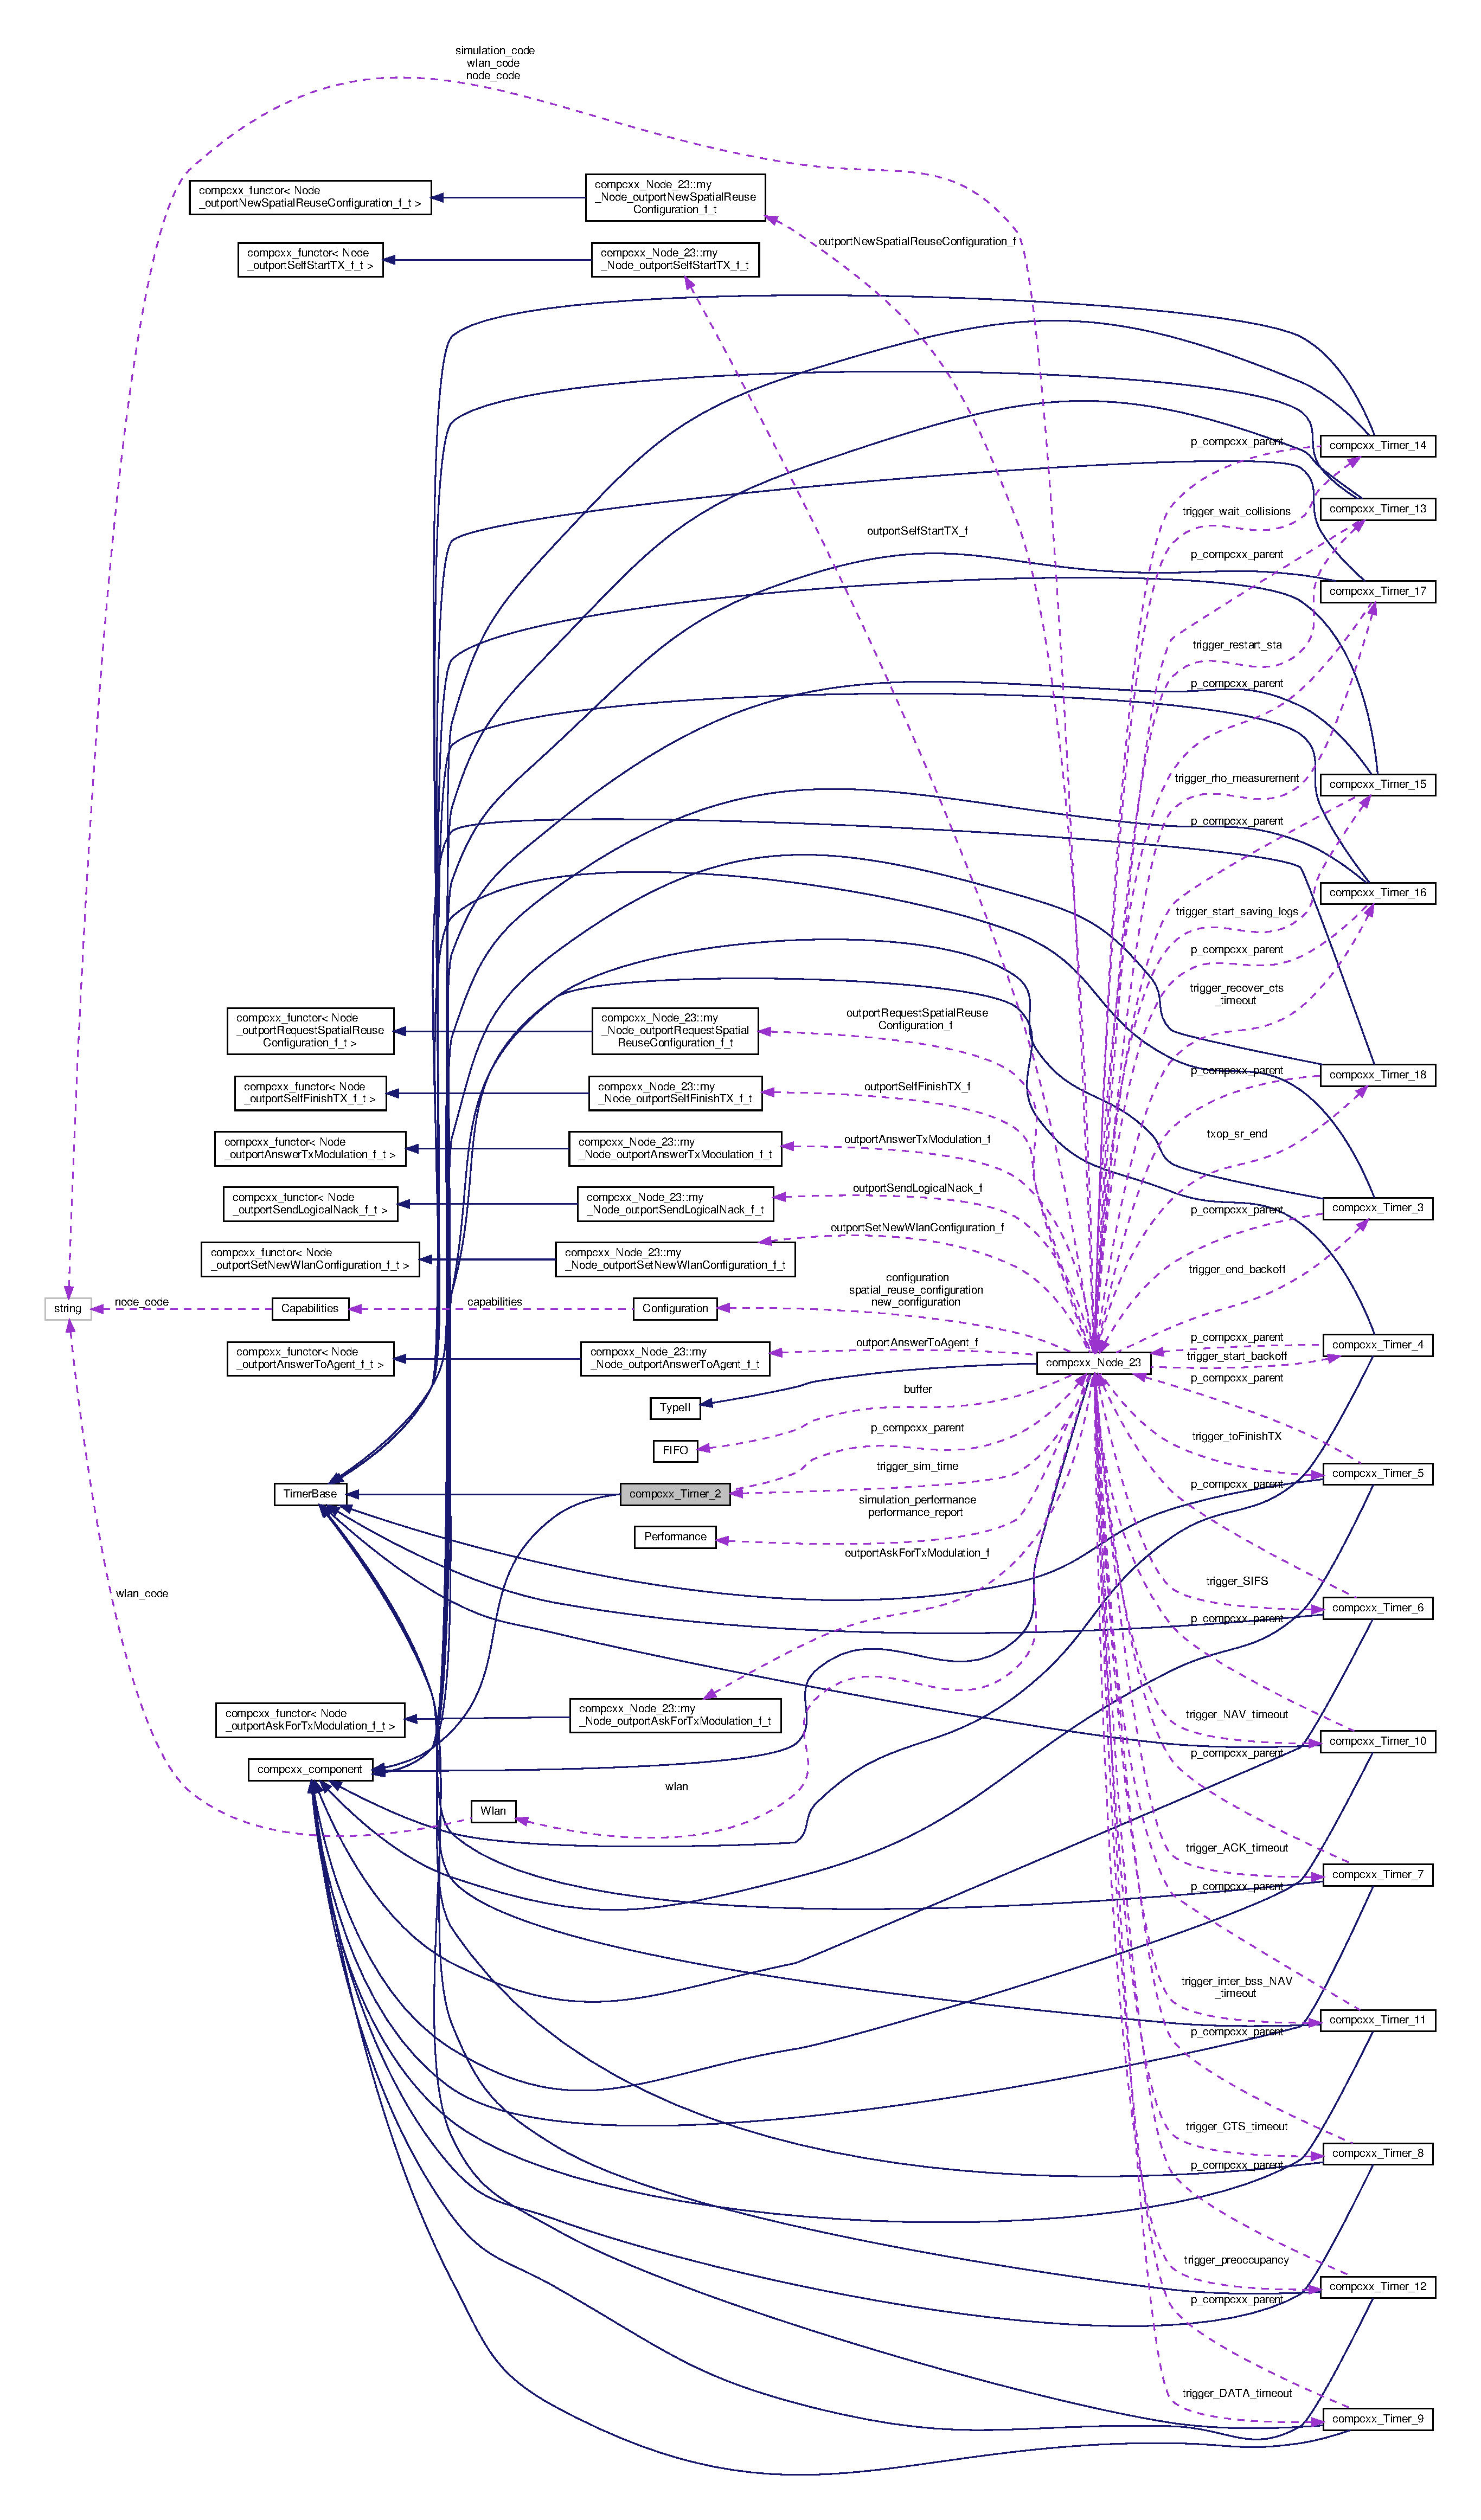
\includegraphics[height=550pt]{classcompcxx__Timer__2__coll__graph}
\end{center}
\end{figure}
\subsection*{Classes}
\begin{DoxyCompactItemize}
\item 
struct \hyperlink{structcompcxx__Timer__2_1_1event__t}{event\+\_\+t}
\end{DoxyCompactItemize}
\subsection*{Public Member Functions}
\begin{DoxyCompactItemize}
\item 
\mbox{\Hypertarget{classcompcxx__Timer__2_a623450dbdb3f43cc745893738e82c6e2}\label{classcompcxx__Timer__2_a623450dbdb3f43cc745893738e82c6e2}} 
void {\bfseries Set} (\hyperlink{classtrigger__t}{trigger\+\_\+t} const \&, double)
\item 
\mbox{\Hypertarget{classcompcxx__Timer__2_a3a72934a86e72c4b75ae8754f345b988}\label{classcompcxx__Timer__2_a3a72934a86e72c4b75ae8754f345b988}} 
void {\bfseries Set} (double)
\item 
\mbox{\Hypertarget{classcompcxx__Timer__2_a6df63ca06bc3179aacadd5ccf476437a}\label{classcompcxx__Timer__2_a6df63ca06bc3179aacadd5ccf476437a}} 
double {\bfseries Get\+Time} ()
\item 
\mbox{\Hypertarget{classcompcxx__Timer__2_ad1e8536bba9565f3c88433196b7e4ccb}\label{classcompcxx__Timer__2_ad1e8536bba9565f3c88433196b7e4ccb}} 
bool {\bfseries Active} ()
\item 
\mbox{\Hypertarget{classcompcxx__Timer__2_ad200ddd850c2d21a73558e5bf7d59bdf}\label{classcompcxx__Timer__2_ad200ddd850c2d21a73558e5bf7d59bdf}} 
\hyperlink{classtrigger__t}{trigger\+\_\+t} \& {\bfseries Get\+Data} ()
\item 
\mbox{\Hypertarget{classcompcxx__Timer__2_a15153698f1cd4a0e398ca5e050892eaa}\label{classcompcxx__Timer__2_a15153698f1cd4a0e398ca5e050892eaa}} 
void {\bfseries Set\+Data} (\hyperlink{classtrigger__t}{trigger\+\_\+t} const \&d)
\item 
\mbox{\Hypertarget{classcompcxx__Timer__2_abdc10b3656fcfd77e8218b5327044ccd}\label{classcompcxx__Timer__2_abdc10b3656fcfd77e8218b5327044ccd}} 
void {\bfseries Cancel} ()
\item 
\mbox{\Hypertarget{classcompcxx__Timer__2_aa425202fb23f28428b46de17a6f3da11}\label{classcompcxx__Timer__2_aa425202fb23f28428b46de17a6f3da11}} 
void {\bfseries activate} (\hyperlink{structCostEvent}{Cost\+Event} $\ast$)
\end{DoxyCompactItemize}
\subsection*{Public Attributes}
\begin{DoxyCompactItemize}
\item 
\mbox{\Hypertarget{classcompcxx__Timer__2_ad280907b9da603e2c6eeba17c2fbdb9f}\label{classcompcxx__Timer__2_ad280907b9da603e2c6eeba17c2fbdb9f}} 
\hyperlink{classcompcxx__Node__23}{compcxx\+\_\+\+Node\+\_\+23} $\ast$ {\bfseries p\+\_\+compcxx\+\_\+parent}
\end{DoxyCompactItemize}
\subsection*{Additional Inherited Members}


The documentation for this class was generated from the following file\+:\begin{DoxyCompactItemize}
\item 
Code/main/komondor\+\_\+main.\+cxx\end{DoxyCompactItemize}

\hypertarget{classcompcxx__Timer__20}{}\section{compcxx\+\_\+\+Timer\+\_\+20 Class Reference}
\label{classcompcxx__Timer__20}\index{compcxx\+\_\+\+Timer\+\_\+20@{compcxx\+\_\+\+Timer\+\_\+20}}


Inheritance diagram for compcxx\+\_\+\+Timer\+\_\+20\+:\nopagebreak
\begin{figure}[H]
\begin{center}
\leavevmode
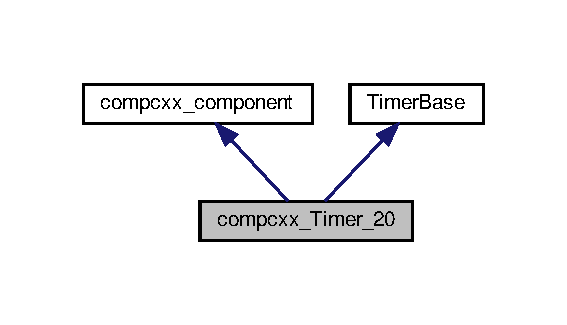
\includegraphics[width=272pt]{classcompcxx__Timer__20__inherit__graph}
\end{center}
\end{figure}


Collaboration diagram for compcxx\+\_\+\+Timer\+\_\+20\+:\nopagebreak
\begin{figure}[H]
\begin{center}
\leavevmode
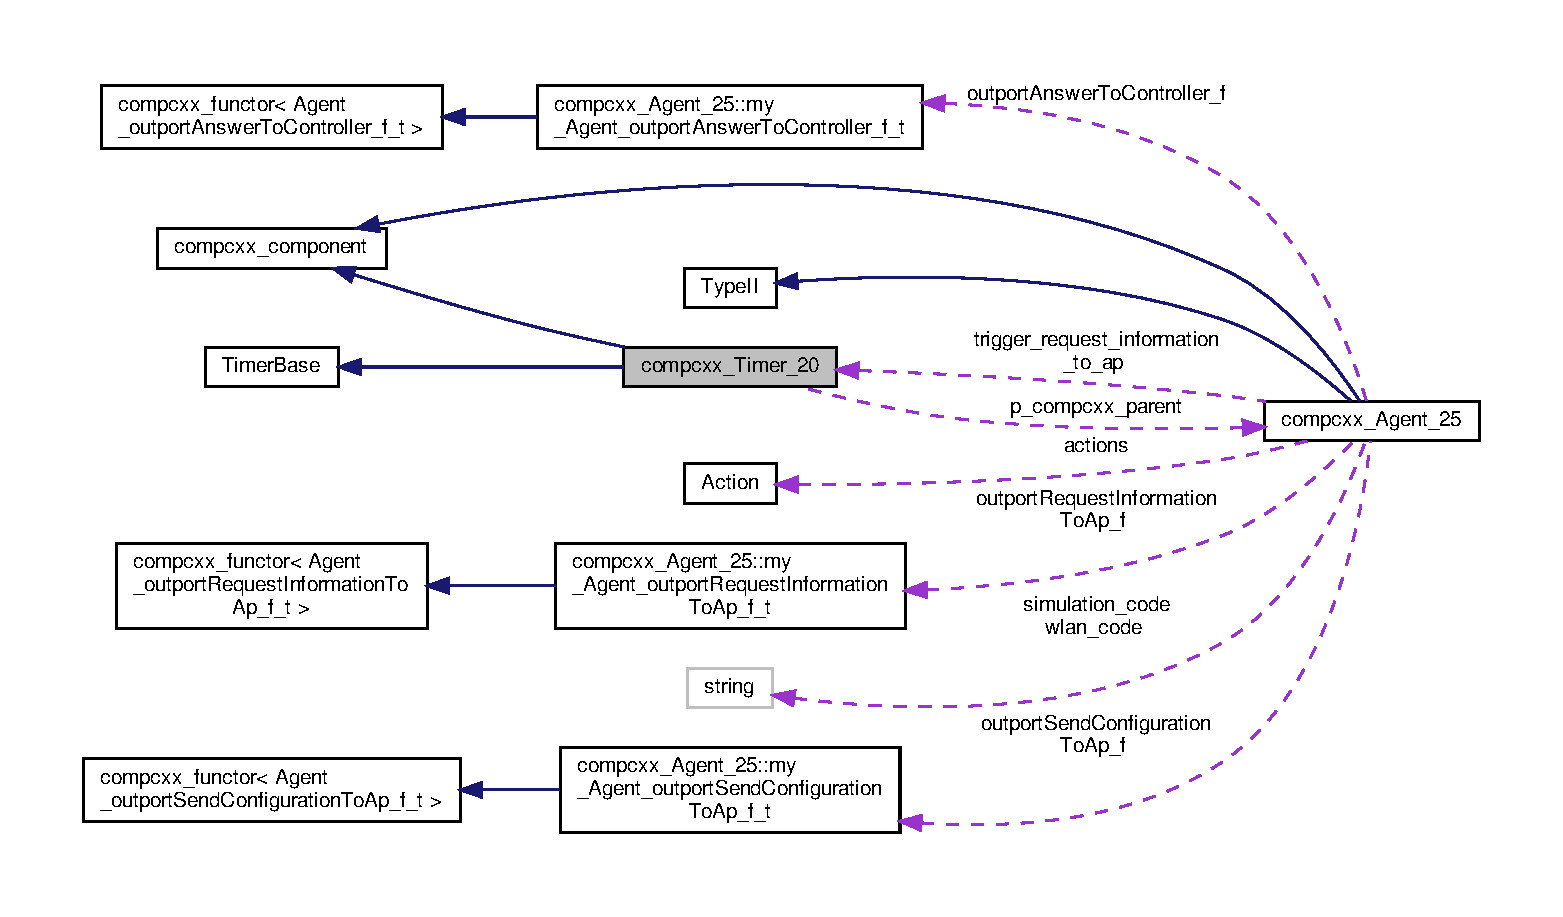
\includegraphics[width=350pt]{classcompcxx__Timer__20__coll__graph}
\end{center}
\end{figure}
\subsection*{Classes}
\begin{DoxyCompactItemize}
\item 
struct \hyperlink{structcompcxx__Timer__20_1_1event__t}{event\+\_\+t}
\end{DoxyCompactItemize}
\subsection*{Public Member Functions}
\begin{DoxyCompactItemize}
\item 
\mbox{\Hypertarget{classcompcxx__Timer__20_ac812a18210553a3499bd781d5754e197}\label{classcompcxx__Timer__20_ac812a18210553a3499bd781d5754e197}} 
void {\bfseries Set} (\hyperlink{classtrigger__t}{trigger\+\_\+t} const \&, double)
\item 
\mbox{\Hypertarget{classcompcxx__Timer__20_a41eddcb43938c37e17b45d870f861d5b}\label{classcompcxx__Timer__20_a41eddcb43938c37e17b45d870f861d5b}} 
void {\bfseries Set} (double)
\item 
\mbox{\Hypertarget{classcompcxx__Timer__20_ad1a7d45984576a86c3e4d021e543e594}\label{classcompcxx__Timer__20_ad1a7d45984576a86c3e4d021e543e594}} 
double {\bfseries Get\+Time} ()
\item 
\mbox{\Hypertarget{classcompcxx__Timer__20_a6ebd529cfacdf50ca9bea8ebf015863c}\label{classcompcxx__Timer__20_a6ebd529cfacdf50ca9bea8ebf015863c}} 
bool {\bfseries Active} ()
\item 
\mbox{\Hypertarget{classcompcxx__Timer__20_a4a1167399fe354c9628f01a0c9efcdb3}\label{classcompcxx__Timer__20_a4a1167399fe354c9628f01a0c9efcdb3}} 
\hyperlink{classtrigger__t}{trigger\+\_\+t} \& {\bfseries Get\+Data} ()
\item 
\mbox{\Hypertarget{classcompcxx__Timer__20_aa6803a6a600210a965a4faede94f8468}\label{classcompcxx__Timer__20_aa6803a6a600210a965a4faede94f8468}} 
void {\bfseries Set\+Data} (\hyperlink{classtrigger__t}{trigger\+\_\+t} const \&d)
\item 
\mbox{\Hypertarget{classcompcxx__Timer__20_a44cb79945992e02ed6ffccb9a7ee6d1e}\label{classcompcxx__Timer__20_a44cb79945992e02ed6ffccb9a7ee6d1e}} 
void {\bfseries Cancel} ()
\item 
\mbox{\Hypertarget{classcompcxx__Timer__20_a5c57b327c1875223f810cde3ec6c0dca}\label{classcompcxx__Timer__20_a5c57b327c1875223f810cde3ec6c0dca}} 
void {\bfseries activate} (\hyperlink{structCostEvent}{Cost\+Event} $\ast$)
\end{DoxyCompactItemize}
\subsection*{Public Attributes}
\begin{DoxyCompactItemize}
\item 
\mbox{\Hypertarget{classcompcxx__Timer__20_a5f333d57effaf858109e5bedd658a12c}\label{classcompcxx__Timer__20_a5f333d57effaf858109e5bedd658a12c}} 
\hyperlink{classcompcxx__Agent__25}{compcxx\+\_\+\+Agent\+\_\+25} $\ast$ {\bfseries p\+\_\+compcxx\+\_\+parent}
\end{DoxyCompactItemize}
\subsection*{Additional Inherited Members}


The documentation for this class was generated from the following file\+:\begin{DoxyCompactItemize}
\item 
Code/main/komondor\+\_\+main.\+cxx\end{DoxyCompactItemize}

\hypertarget{classcompcxx__Timer__21}{}\section{compcxx\+\_\+\+Timer\+\_\+21 Class Reference}
\label{classcompcxx__Timer__21}\index{compcxx\+\_\+\+Timer\+\_\+21@{compcxx\+\_\+\+Timer\+\_\+21}}


Inheritance diagram for compcxx\+\_\+\+Timer\+\_\+21\+:\nopagebreak
\begin{figure}[H]
\begin{center}
\leavevmode
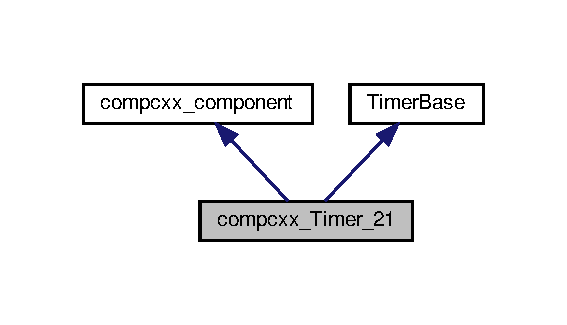
\includegraphics[width=272pt]{classcompcxx__Timer__21__inherit__graph}
\end{center}
\end{figure}


Collaboration diagram for compcxx\+\_\+\+Timer\+\_\+21\+:\nopagebreak
\begin{figure}[H]
\begin{center}
\leavevmode
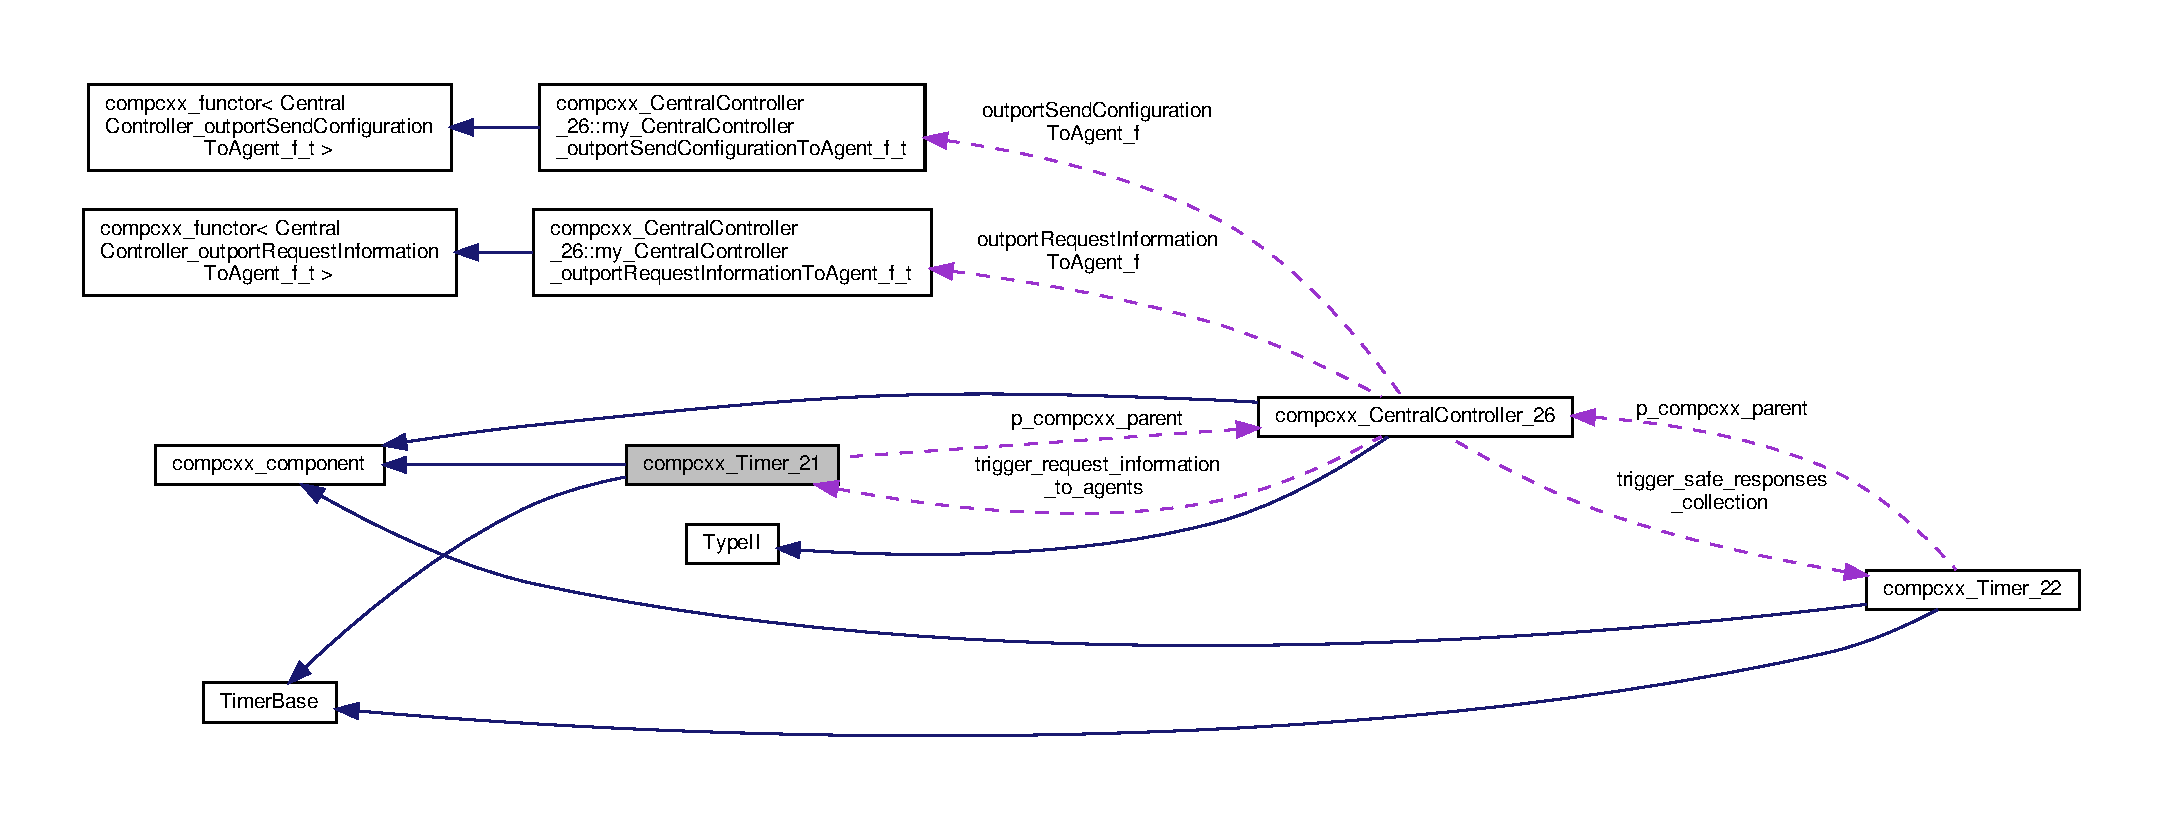
\includegraphics[width=350pt]{classcompcxx__Timer__21__coll__graph}
\end{center}
\end{figure}
\subsection*{Classes}
\begin{DoxyCompactItemize}
\item 
struct \hyperlink{structcompcxx__Timer__21_1_1event__t}{event\+\_\+t}
\end{DoxyCompactItemize}
\subsection*{Public Member Functions}
\begin{DoxyCompactItemize}
\item 
\mbox{\Hypertarget{classcompcxx__Timer__21_abc7a7464c16fbb360e74acfd3e38a395}\label{classcompcxx__Timer__21_abc7a7464c16fbb360e74acfd3e38a395}} 
void {\bfseries Set} (\hyperlink{classtrigger__t}{trigger\+\_\+t} const \&, double)
\item 
\mbox{\Hypertarget{classcompcxx__Timer__21_aacdf5f8df7d954948f656109438de37c}\label{classcompcxx__Timer__21_aacdf5f8df7d954948f656109438de37c}} 
void {\bfseries Set} (double)
\item 
\mbox{\Hypertarget{classcompcxx__Timer__21_ac23543f9ec46482859efeb6c2e890a1a}\label{classcompcxx__Timer__21_ac23543f9ec46482859efeb6c2e890a1a}} 
double {\bfseries Get\+Time} ()
\item 
\mbox{\Hypertarget{classcompcxx__Timer__21_af28073033d996abb5e570a3e0dc3a0b3}\label{classcompcxx__Timer__21_af28073033d996abb5e570a3e0dc3a0b3}} 
bool {\bfseries Active} ()
\item 
\mbox{\Hypertarget{classcompcxx__Timer__21_a3722004e3dc846326c343dd80f5008c2}\label{classcompcxx__Timer__21_a3722004e3dc846326c343dd80f5008c2}} 
\hyperlink{classtrigger__t}{trigger\+\_\+t} \& {\bfseries Get\+Data} ()
\item 
\mbox{\Hypertarget{classcompcxx__Timer__21_ad7c8fe681b70eb7d17abe31789f0c569}\label{classcompcxx__Timer__21_ad7c8fe681b70eb7d17abe31789f0c569}} 
void {\bfseries Set\+Data} (\hyperlink{classtrigger__t}{trigger\+\_\+t} const \&d)
\item 
\mbox{\Hypertarget{classcompcxx__Timer__21_a8cd0fc84c3b7af9eaba2650a469613ae}\label{classcompcxx__Timer__21_a8cd0fc84c3b7af9eaba2650a469613ae}} 
void {\bfseries Cancel} ()
\item 
\mbox{\Hypertarget{classcompcxx__Timer__21_a283f0689f0e4678ff2e6adf2d398b43f}\label{classcompcxx__Timer__21_a283f0689f0e4678ff2e6adf2d398b43f}} 
void {\bfseries activate} (\hyperlink{structCostEvent}{Cost\+Event} $\ast$)
\end{DoxyCompactItemize}
\subsection*{Public Attributes}
\begin{DoxyCompactItemize}
\item 
\mbox{\Hypertarget{classcompcxx__Timer__21_a498b85c8aac6e24bbfa2576bca6057f5}\label{classcompcxx__Timer__21_a498b85c8aac6e24bbfa2576bca6057f5}} 
\hyperlink{classcompcxx__CentralController__26}{compcxx\+\_\+\+Central\+Controller\+\_\+26} $\ast$ {\bfseries p\+\_\+compcxx\+\_\+parent}
\end{DoxyCompactItemize}
\subsection*{Additional Inherited Members}


The documentation for this class was generated from the following file\+:\begin{DoxyCompactItemize}
\item 
Code/main/komondor\+\_\+main.\+cxx\end{DoxyCompactItemize}

\hypertarget{classcompcxx__Timer__22}{}\section{compcxx\+\_\+\+Timer\+\_\+22 Class Reference}
\label{classcompcxx__Timer__22}\index{compcxx\+\_\+\+Timer\+\_\+22@{compcxx\+\_\+\+Timer\+\_\+22}}


Inheritance diagram for compcxx\+\_\+\+Timer\+\_\+22\+:\nopagebreak
\begin{figure}[H]
\begin{center}
\leavevmode
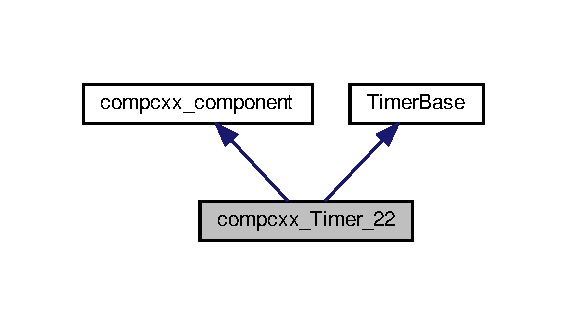
\includegraphics[width=272pt]{classcompcxx__Timer__22__inherit__graph}
\end{center}
\end{figure}


Collaboration diagram for compcxx\+\_\+\+Timer\+\_\+22\+:\nopagebreak
\begin{figure}[H]
\begin{center}
\leavevmode
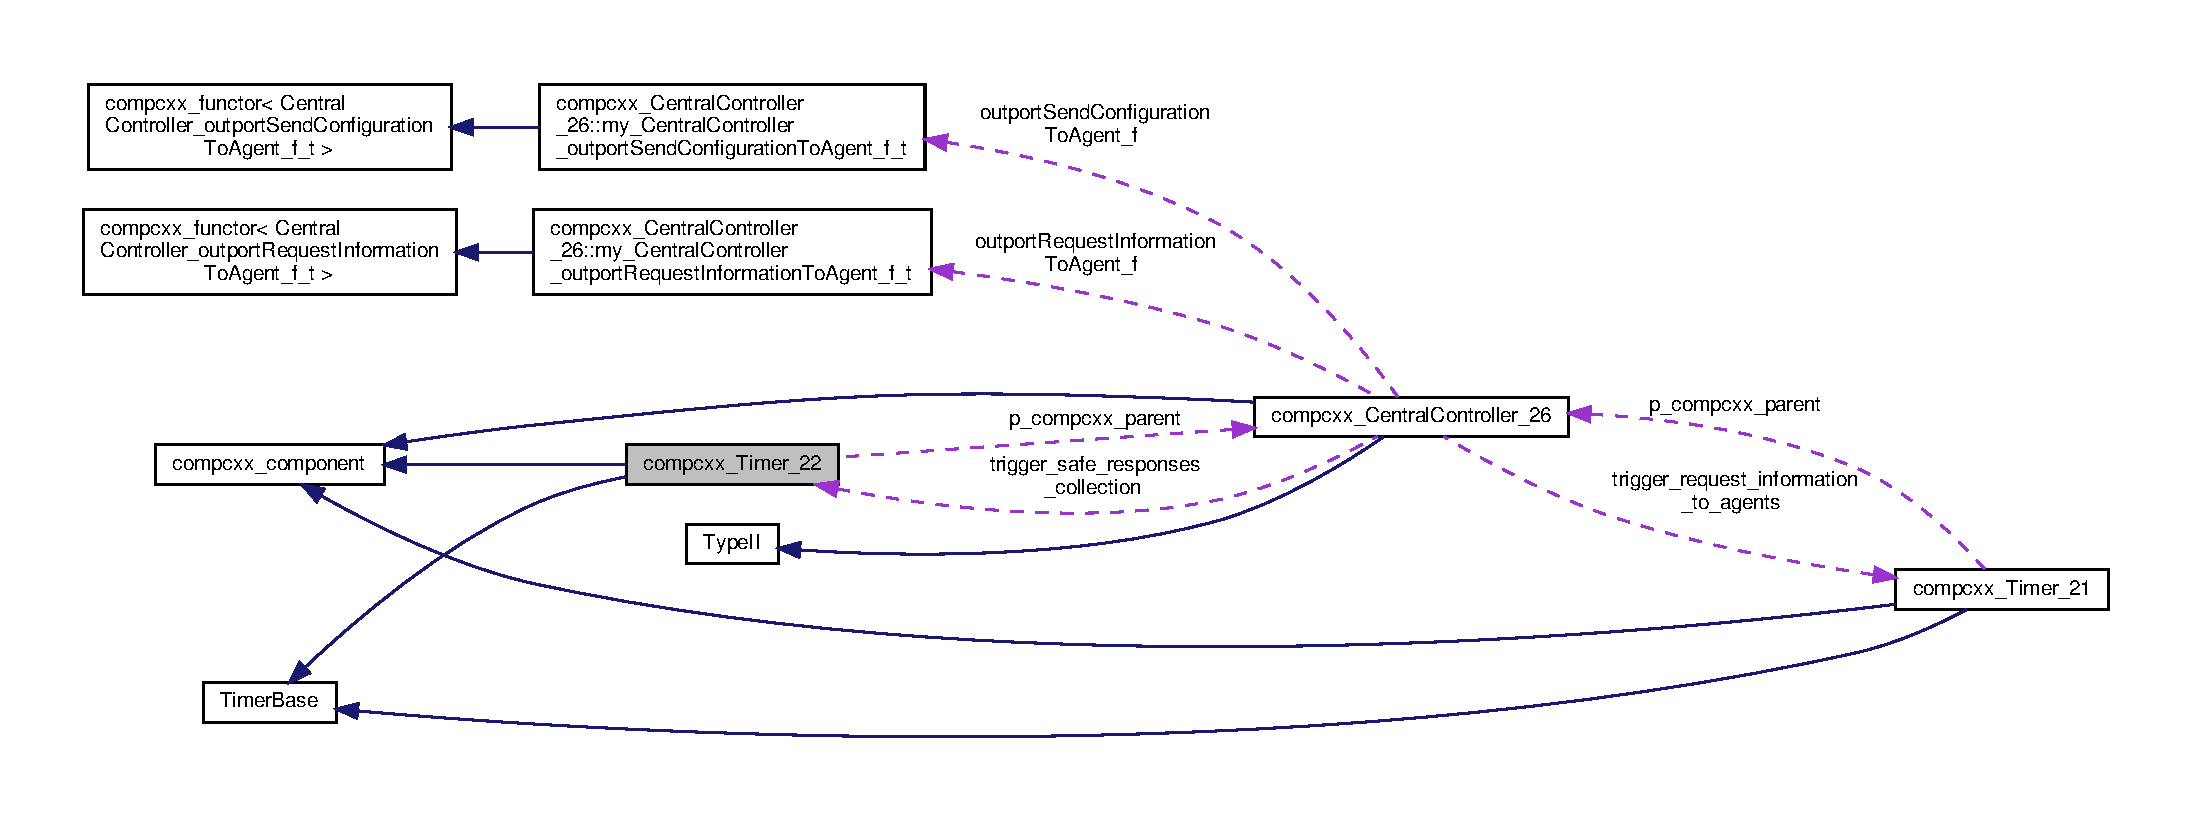
\includegraphics[width=350pt]{classcompcxx__Timer__22__coll__graph}
\end{center}
\end{figure}
\subsection*{Classes}
\begin{DoxyCompactItemize}
\item 
struct \hyperlink{structcompcxx__Timer__22_1_1event__t}{event\+\_\+t}
\end{DoxyCompactItemize}
\subsection*{Public Member Functions}
\begin{DoxyCompactItemize}
\item 
\mbox{\Hypertarget{classcompcxx__Timer__22_ac29a6402c29603b206d7a05f880ce837}\label{classcompcxx__Timer__22_ac29a6402c29603b206d7a05f880ce837}} 
void {\bfseries Set} (\hyperlink{classtrigger__t}{trigger\+\_\+t} const \&, double)
\item 
\mbox{\Hypertarget{classcompcxx__Timer__22_aa9237014c12d6e581aeedbe7c2c6718e}\label{classcompcxx__Timer__22_aa9237014c12d6e581aeedbe7c2c6718e}} 
void {\bfseries Set} (double)
\item 
\mbox{\Hypertarget{classcompcxx__Timer__22_a3d5db413931a94f7f3e1657fe6db4d58}\label{classcompcxx__Timer__22_a3d5db413931a94f7f3e1657fe6db4d58}} 
double {\bfseries Get\+Time} ()
\item 
\mbox{\Hypertarget{classcompcxx__Timer__22_afd87b916902eb89dbd483ed0bc2c6c95}\label{classcompcxx__Timer__22_afd87b916902eb89dbd483ed0bc2c6c95}} 
bool {\bfseries Active} ()
\item 
\mbox{\Hypertarget{classcompcxx__Timer__22_a43737285477d126eca775306bbd6283c}\label{classcompcxx__Timer__22_a43737285477d126eca775306bbd6283c}} 
\hyperlink{classtrigger__t}{trigger\+\_\+t} \& {\bfseries Get\+Data} ()
\item 
\mbox{\Hypertarget{classcompcxx__Timer__22_a604bcc01ec601c6f7163a23c91582407}\label{classcompcxx__Timer__22_a604bcc01ec601c6f7163a23c91582407}} 
void {\bfseries Set\+Data} (\hyperlink{classtrigger__t}{trigger\+\_\+t} const \&d)
\item 
\mbox{\Hypertarget{classcompcxx__Timer__22_aac4833497950f060a68b82a0115eee95}\label{classcompcxx__Timer__22_aac4833497950f060a68b82a0115eee95}} 
void {\bfseries Cancel} ()
\item 
\mbox{\Hypertarget{classcompcxx__Timer__22_a22700ca654795698a78f94708d1c422f}\label{classcompcxx__Timer__22_a22700ca654795698a78f94708d1c422f}} 
void {\bfseries activate} (\hyperlink{structCostEvent}{Cost\+Event} $\ast$)
\end{DoxyCompactItemize}
\subsection*{Public Attributes}
\begin{DoxyCompactItemize}
\item 
\mbox{\Hypertarget{classcompcxx__Timer__22_a77f891a2a289ceac4012c8864abcb675}\label{classcompcxx__Timer__22_a77f891a2a289ceac4012c8864abcb675}} 
\hyperlink{classcompcxx__CentralController__26}{compcxx\+\_\+\+Central\+Controller\+\_\+26} $\ast$ {\bfseries p\+\_\+compcxx\+\_\+parent}
\end{DoxyCompactItemize}
\subsection*{Additional Inherited Members}


The documentation for this class was generated from the following file\+:\begin{DoxyCompactItemize}
\item 
Code/main/komondor\+\_\+main.\+cxx\end{DoxyCompactItemize}

\hypertarget{classcompcxx__Timer__3}{}\section{compcxx\+\_\+\+Timer\+\_\+3 Class Reference}
\label{classcompcxx__Timer__3}\index{compcxx\+\_\+\+Timer\+\_\+3@{compcxx\+\_\+\+Timer\+\_\+3}}


Inheritance diagram for compcxx\+\_\+\+Timer\+\_\+3\+:\nopagebreak
\begin{figure}[H]
\begin{center}
\leavevmode
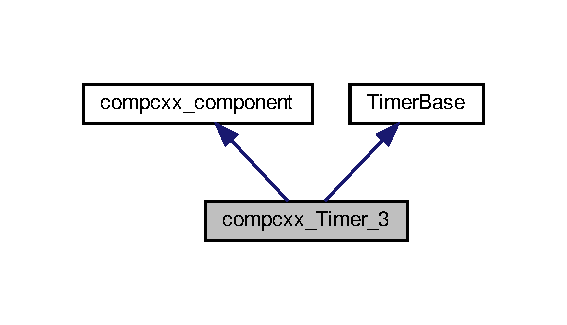
\includegraphics[width=272pt]{classcompcxx__Timer__3__inherit__graph}
\end{center}
\end{figure}


Collaboration diagram for compcxx\+\_\+\+Timer\+\_\+3\+:\nopagebreak
\begin{figure}[H]
\begin{center}
\leavevmode
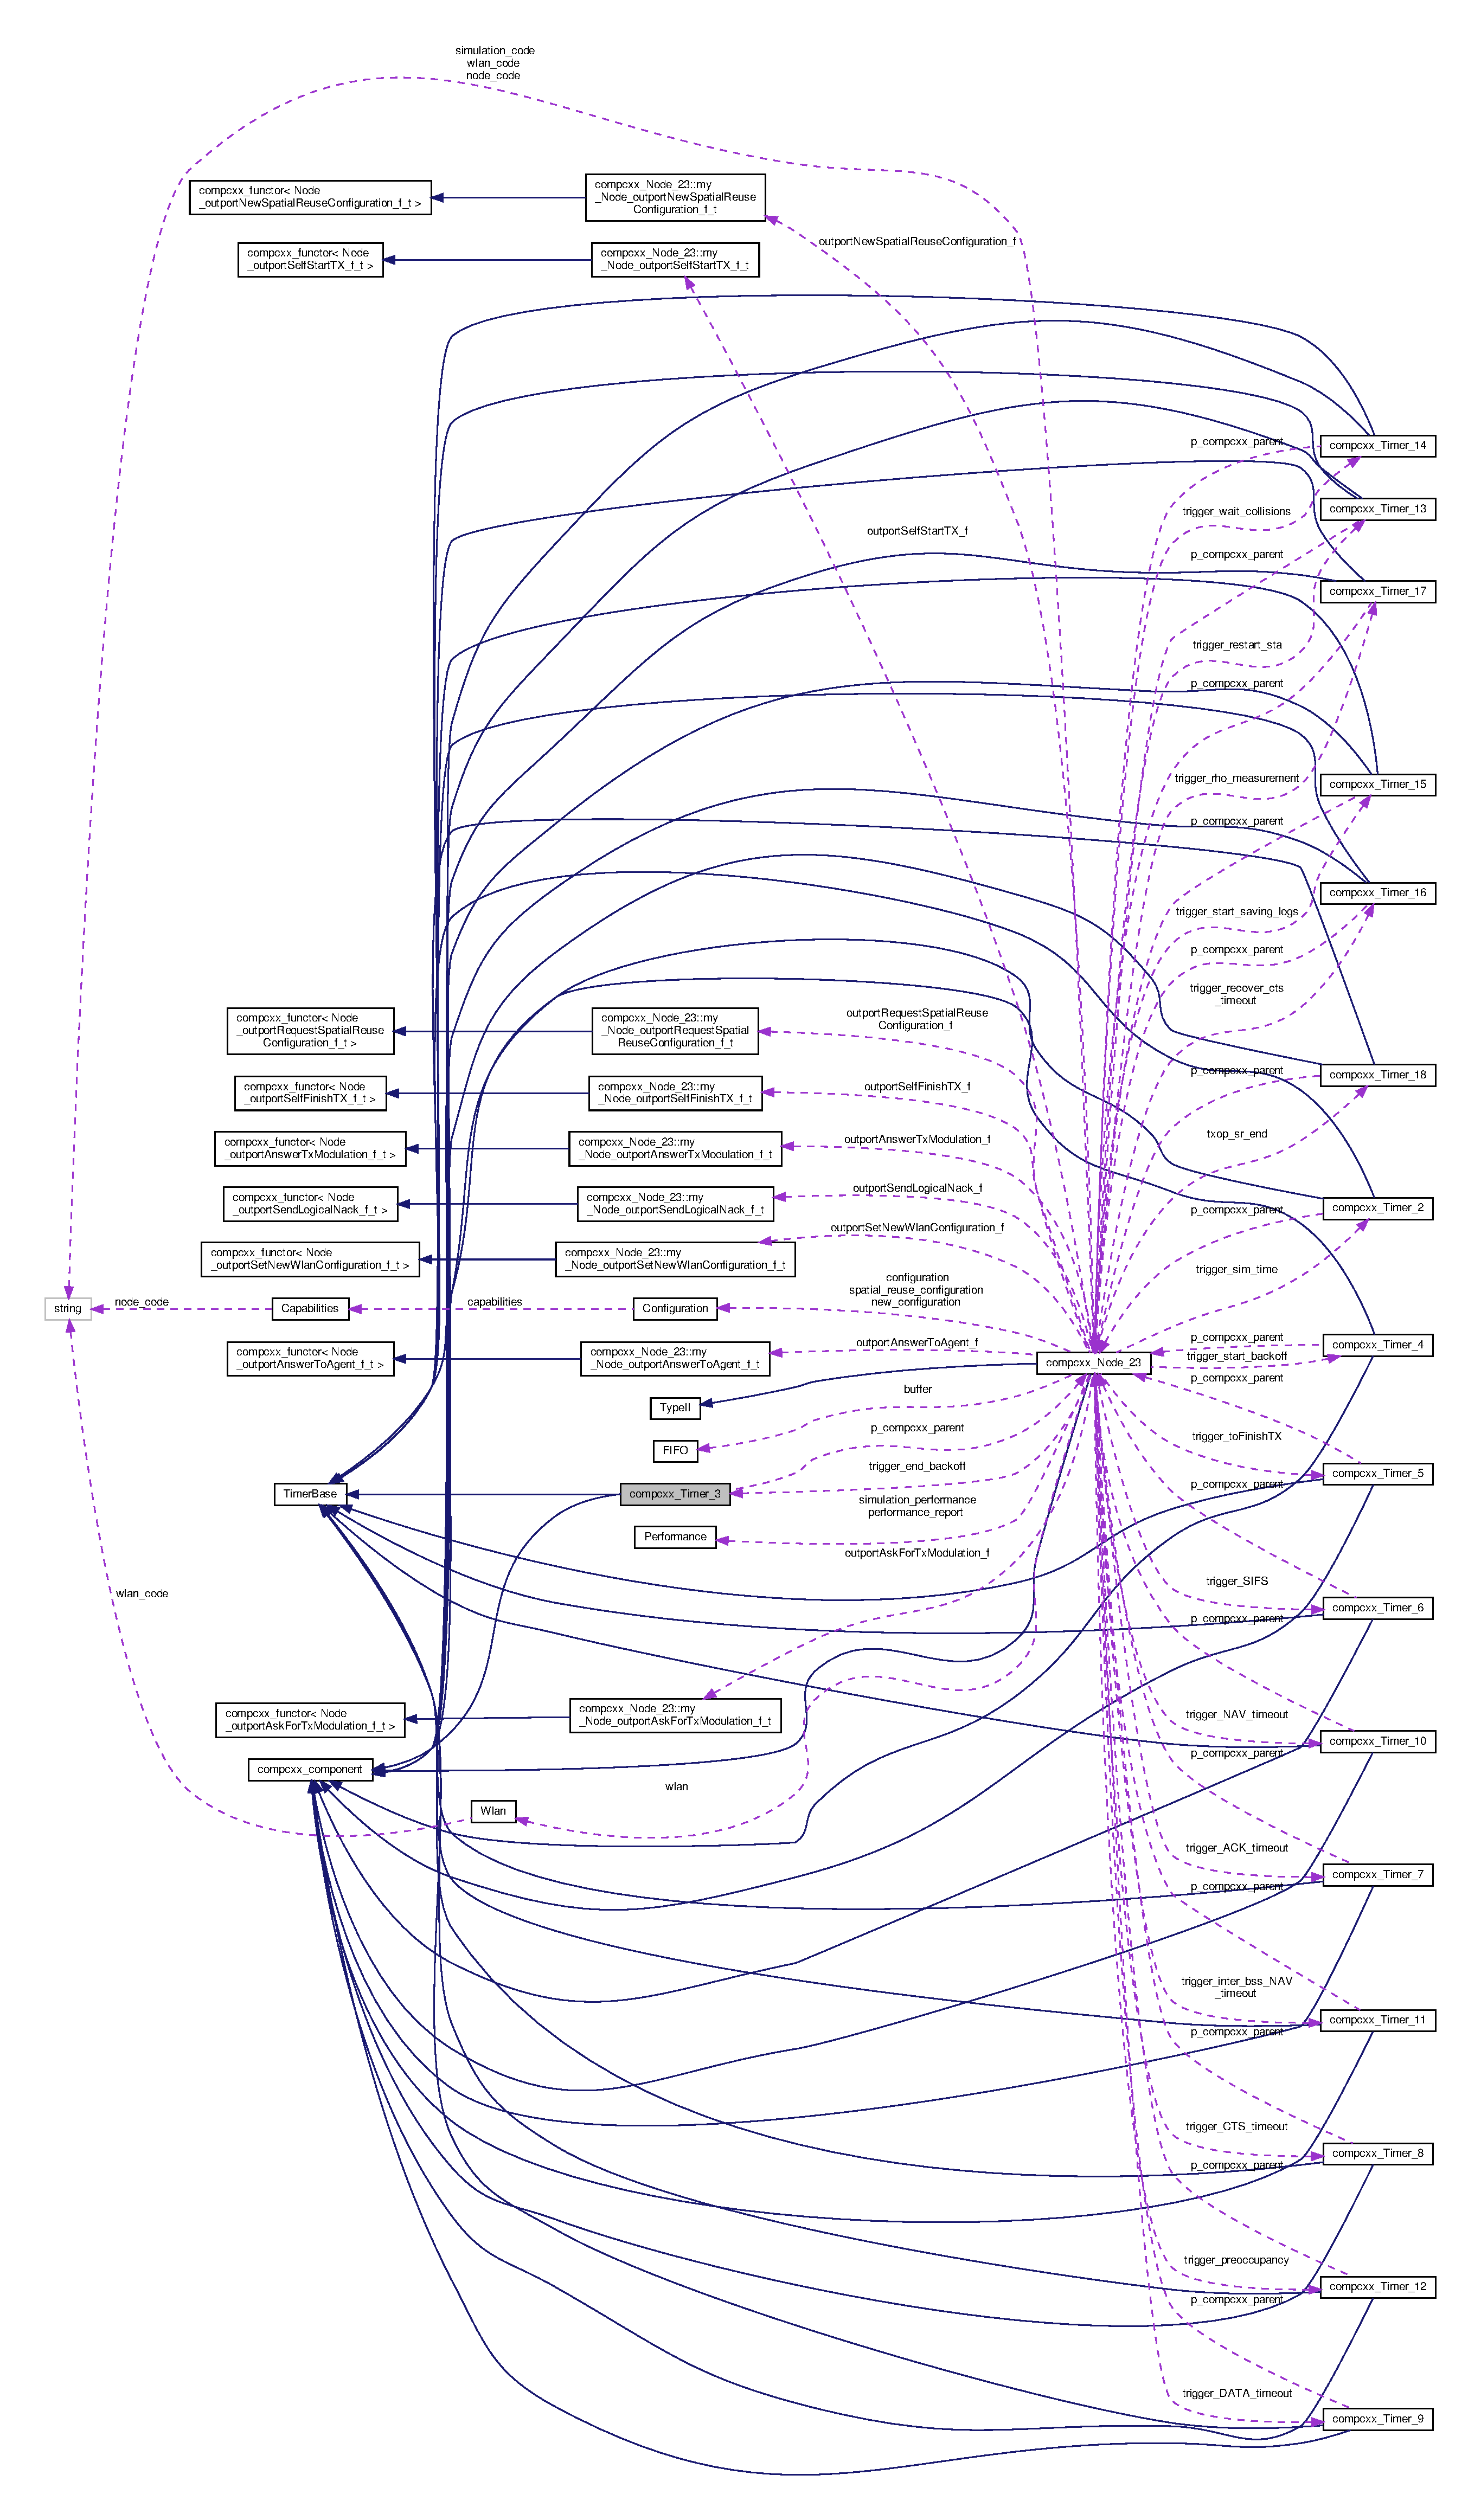
\includegraphics[height=550pt]{classcompcxx__Timer__3__coll__graph}
\end{center}
\end{figure}
\subsection*{Classes}
\begin{DoxyCompactItemize}
\item 
struct \hyperlink{structcompcxx__Timer__3_1_1event__t}{event\+\_\+t}
\end{DoxyCompactItemize}
\subsection*{Public Member Functions}
\begin{DoxyCompactItemize}
\item 
\mbox{\Hypertarget{classcompcxx__Timer__3_a0875dfa09e862cbf15e7221bee1cf7c3}\label{classcompcxx__Timer__3_a0875dfa09e862cbf15e7221bee1cf7c3}} 
void {\bfseries Set} (\hyperlink{classtrigger__t}{trigger\+\_\+t} const \&, double)
\item 
\mbox{\Hypertarget{classcompcxx__Timer__3_a5e1d040221ba8f97ae3e1b4df1e126b4}\label{classcompcxx__Timer__3_a5e1d040221ba8f97ae3e1b4df1e126b4}} 
void {\bfseries Set} (double)
\item 
\mbox{\Hypertarget{classcompcxx__Timer__3_a75b12aee8062bfa761fcff1ff4c073d9}\label{classcompcxx__Timer__3_a75b12aee8062bfa761fcff1ff4c073d9}} 
double {\bfseries Get\+Time} ()
\item 
\mbox{\Hypertarget{classcompcxx__Timer__3_afcd4bbc1282ef86e58bd4f8928ae528d}\label{classcompcxx__Timer__3_afcd4bbc1282ef86e58bd4f8928ae528d}} 
bool {\bfseries Active} ()
\item 
\mbox{\Hypertarget{classcompcxx__Timer__3_ae60330a89cf77c270455b78e270211f2}\label{classcompcxx__Timer__3_ae60330a89cf77c270455b78e270211f2}} 
\hyperlink{classtrigger__t}{trigger\+\_\+t} \& {\bfseries Get\+Data} ()
\item 
\mbox{\Hypertarget{classcompcxx__Timer__3_a0e3686756ffb560f54378a5d564b2e03}\label{classcompcxx__Timer__3_a0e3686756ffb560f54378a5d564b2e03}} 
void {\bfseries Set\+Data} (\hyperlink{classtrigger__t}{trigger\+\_\+t} const \&d)
\item 
\mbox{\Hypertarget{classcompcxx__Timer__3_a873e1eb19b4fd894d4775c4a698c6fd9}\label{classcompcxx__Timer__3_a873e1eb19b4fd894d4775c4a698c6fd9}} 
void {\bfseries Cancel} ()
\item 
\mbox{\Hypertarget{classcompcxx__Timer__3_aa37e7cdf36c9d1214481935ee579787b}\label{classcompcxx__Timer__3_aa37e7cdf36c9d1214481935ee579787b}} 
void {\bfseries activate} (\hyperlink{structCostEvent}{Cost\+Event} $\ast$)
\end{DoxyCompactItemize}
\subsection*{Public Attributes}
\begin{DoxyCompactItemize}
\item 
\mbox{\Hypertarget{classcompcxx__Timer__3_a044d5904b86a2b9b44d9d084c9a03bd2}\label{classcompcxx__Timer__3_a044d5904b86a2b9b44d9d084c9a03bd2}} 
\hyperlink{classcompcxx__Node__23}{compcxx\+\_\+\+Node\+\_\+23} $\ast$ {\bfseries p\+\_\+compcxx\+\_\+parent}
\end{DoxyCompactItemize}
\subsection*{Additional Inherited Members}


The documentation for this class was generated from the following file\+:\begin{DoxyCompactItemize}
\item 
Code/main/komondor\+\_\+main.\+cxx\end{DoxyCompactItemize}

\hypertarget{classcompcxx__Timer__4}{}\section{compcxx\+\_\+\+Timer\+\_\+4 Class Reference}
\label{classcompcxx__Timer__4}\index{compcxx\+\_\+\+Timer\+\_\+4@{compcxx\+\_\+\+Timer\+\_\+4}}


Inheritance diagram for compcxx\+\_\+\+Timer\+\_\+4\+:\nopagebreak
\begin{figure}[H]
\begin{center}
\leavevmode
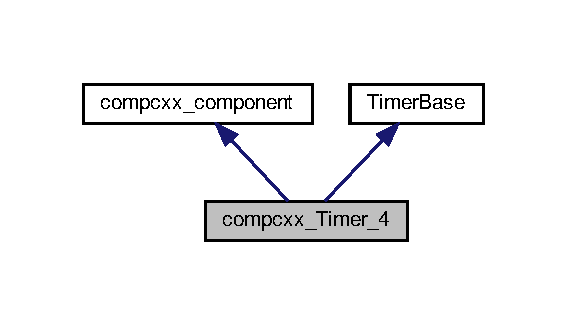
\includegraphics[width=272pt]{classcompcxx__Timer__4__inherit__graph}
\end{center}
\end{figure}


Collaboration diagram for compcxx\+\_\+\+Timer\+\_\+4\+:\nopagebreak
\begin{figure}[H]
\begin{center}
\leavevmode
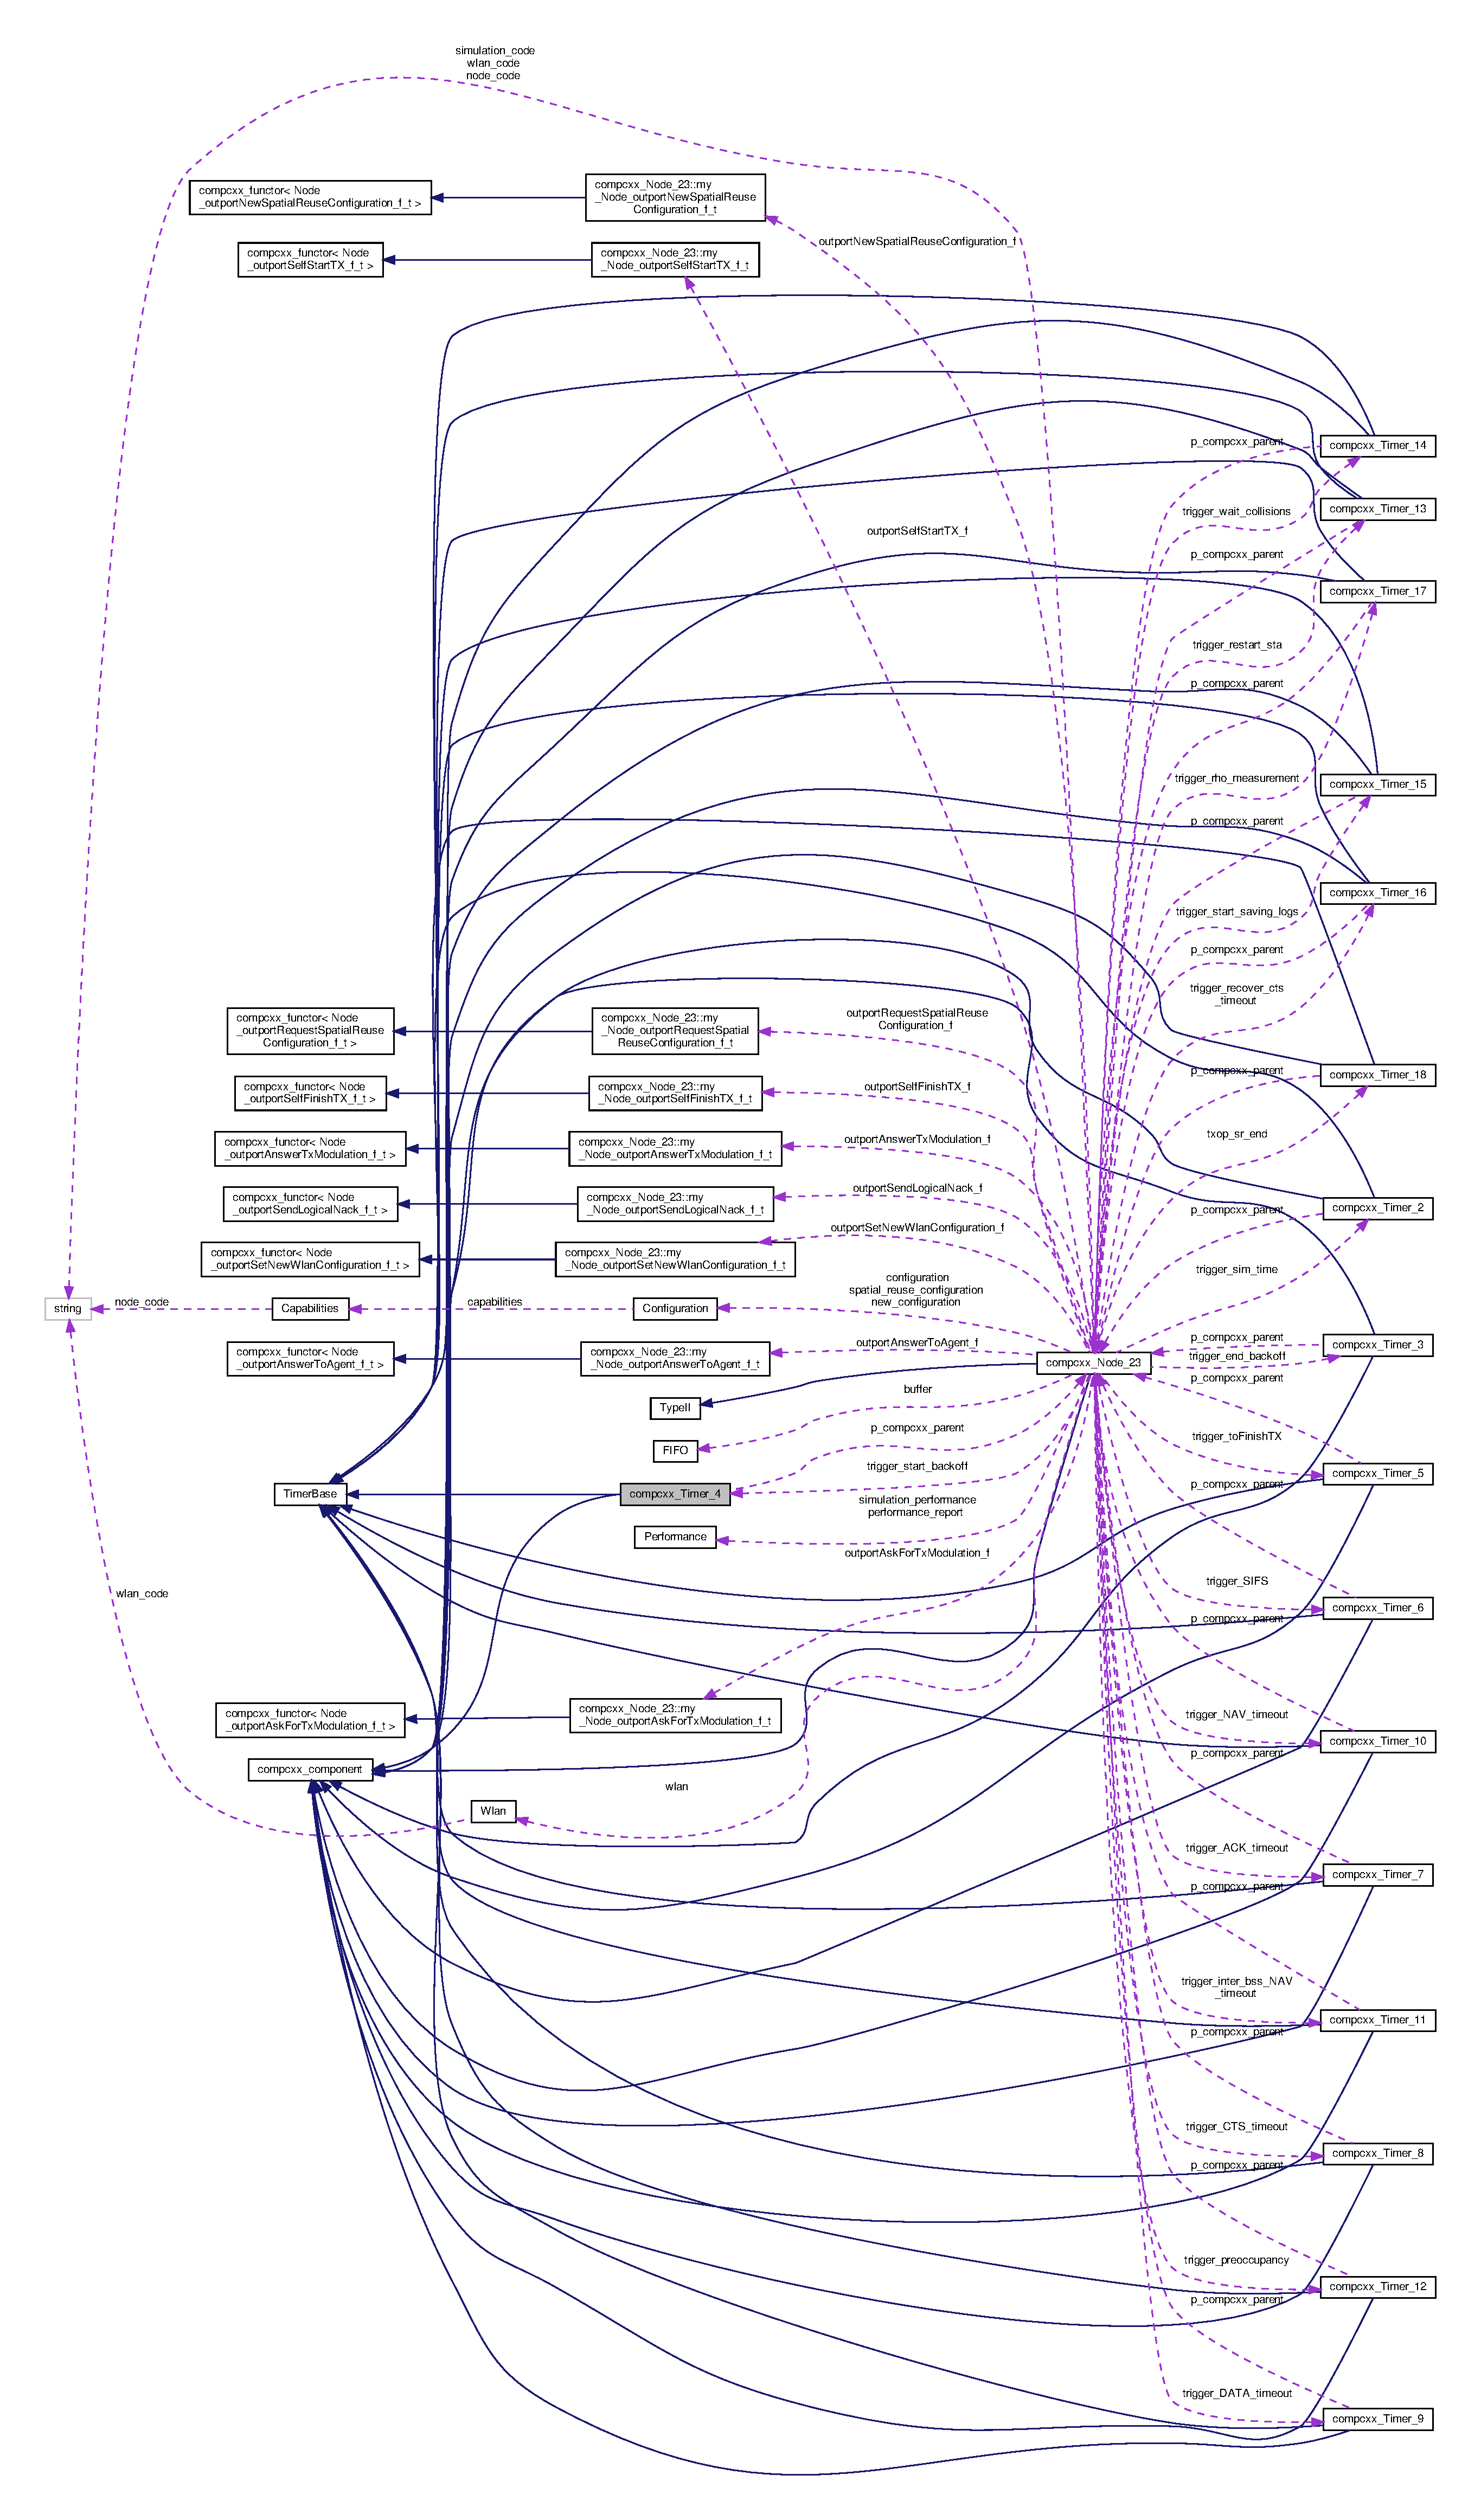
\includegraphics[height=550pt]{classcompcxx__Timer__4__coll__graph}
\end{center}
\end{figure}
\subsection*{Classes}
\begin{DoxyCompactItemize}
\item 
struct \hyperlink{structcompcxx__Timer__4_1_1event__t}{event\+\_\+t}
\end{DoxyCompactItemize}
\subsection*{Public Member Functions}
\begin{DoxyCompactItemize}
\item 
\mbox{\Hypertarget{classcompcxx__Timer__4_aa344d53a945412b225d373e5d3cad0d0}\label{classcompcxx__Timer__4_aa344d53a945412b225d373e5d3cad0d0}} 
void {\bfseries Set} (\hyperlink{classtrigger__t}{trigger\+\_\+t} const \&, double)
\item 
\mbox{\Hypertarget{classcompcxx__Timer__4_aecf41f43bf079714fd788d5bccd64ed8}\label{classcompcxx__Timer__4_aecf41f43bf079714fd788d5bccd64ed8}} 
void {\bfseries Set} (double)
\item 
\mbox{\Hypertarget{classcompcxx__Timer__4_ac22263c8d3c100974d13556887e09d53}\label{classcompcxx__Timer__4_ac22263c8d3c100974d13556887e09d53}} 
double {\bfseries Get\+Time} ()
\item 
\mbox{\Hypertarget{classcompcxx__Timer__4_a02adbf1cc2147f3663e24d7e1656021f}\label{classcompcxx__Timer__4_a02adbf1cc2147f3663e24d7e1656021f}} 
bool {\bfseries Active} ()
\item 
\mbox{\Hypertarget{classcompcxx__Timer__4_a8265158c22f858cd23d9433aa756015f}\label{classcompcxx__Timer__4_a8265158c22f858cd23d9433aa756015f}} 
\hyperlink{classtrigger__t}{trigger\+\_\+t} \& {\bfseries Get\+Data} ()
\item 
\mbox{\Hypertarget{classcompcxx__Timer__4_acbc1687e64daa83ad6542d7bcaf758e5}\label{classcompcxx__Timer__4_acbc1687e64daa83ad6542d7bcaf758e5}} 
void {\bfseries Set\+Data} (\hyperlink{classtrigger__t}{trigger\+\_\+t} const \&d)
\item 
\mbox{\Hypertarget{classcompcxx__Timer__4_a32c02ba3106f47f88b7196ec8cc6677a}\label{classcompcxx__Timer__4_a32c02ba3106f47f88b7196ec8cc6677a}} 
void {\bfseries Cancel} ()
\item 
\mbox{\Hypertarget{classcompcxx__Timer__4_a9f02b98720c5cfd1e87f1fc85bf1622b}\label{classcompcxx__Timer__4_a9f02b98720c5cfd1e87f1fc85bf1622b}} 
void {\bfseries activate} (\hyperlink{structCostEvent}{Cost\+Event} $\ast$)
\end{DoxyCompactItemize}
\subsection*{Public Attributes}
\begin{DoxyCompactItemize}
\item 
\mbox{\Hypertarget{classcompcxx__Timer__4_a4c8a9b7dfdb92654964b43c42dba7f82}\label{classcompcxx__Timer__4_a4c8a9b7dfdb92654964b43c42dba7f82}} 
\hyperlink{classcompcxx__Node__23}{compcxx\+\_\+\+Node\+\_\+23} $\ast$ {\bfseries p\+\_\+compcxx\+\_\+parent}
\end{DoxyCompactItemize}
\subsection*{Additional Inherited Members}


The documentation for this class was generated from the following file\+:\begin{DoxyCompactItemize}
\item 
Code/main/komondor\+\_\+main.\+cxx\end{DoxyCompactItemize}

\hypertarget{classcompcxx__Timer__5}{}\section{compcxx\+\_\+\+Timer\+\_\+5 Class Reference}
\label{classcompcxx__Timer__5}\index{compcxx\+\_\+\+Timer\+\_\+5@{compcxx\+\_\+\+Timer\+\_\+5}}


Inheritance diagram for compcxx\+\_\+\+Timer\+\_\+5\+:\nopagebreak
\begin{figure}[H]
\begin{center}
\leavevmode
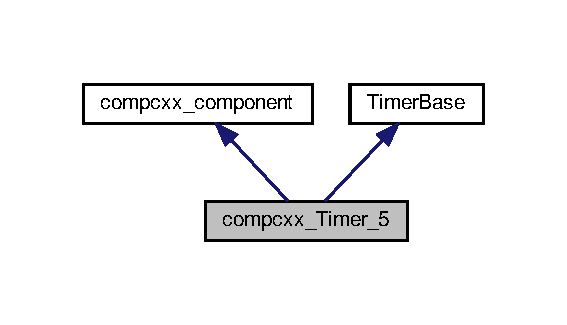
\includegraphics[width=272pt]{classcompcxx__Timer__5__inherit__graph}
\end{center}
\end{figure}


Collaboration diagram for compcxx\+\_\+\+Timer\+\_\+5\+:\nopagebreak
\begin{figure}[H]
\begin{center}
\leavevmode
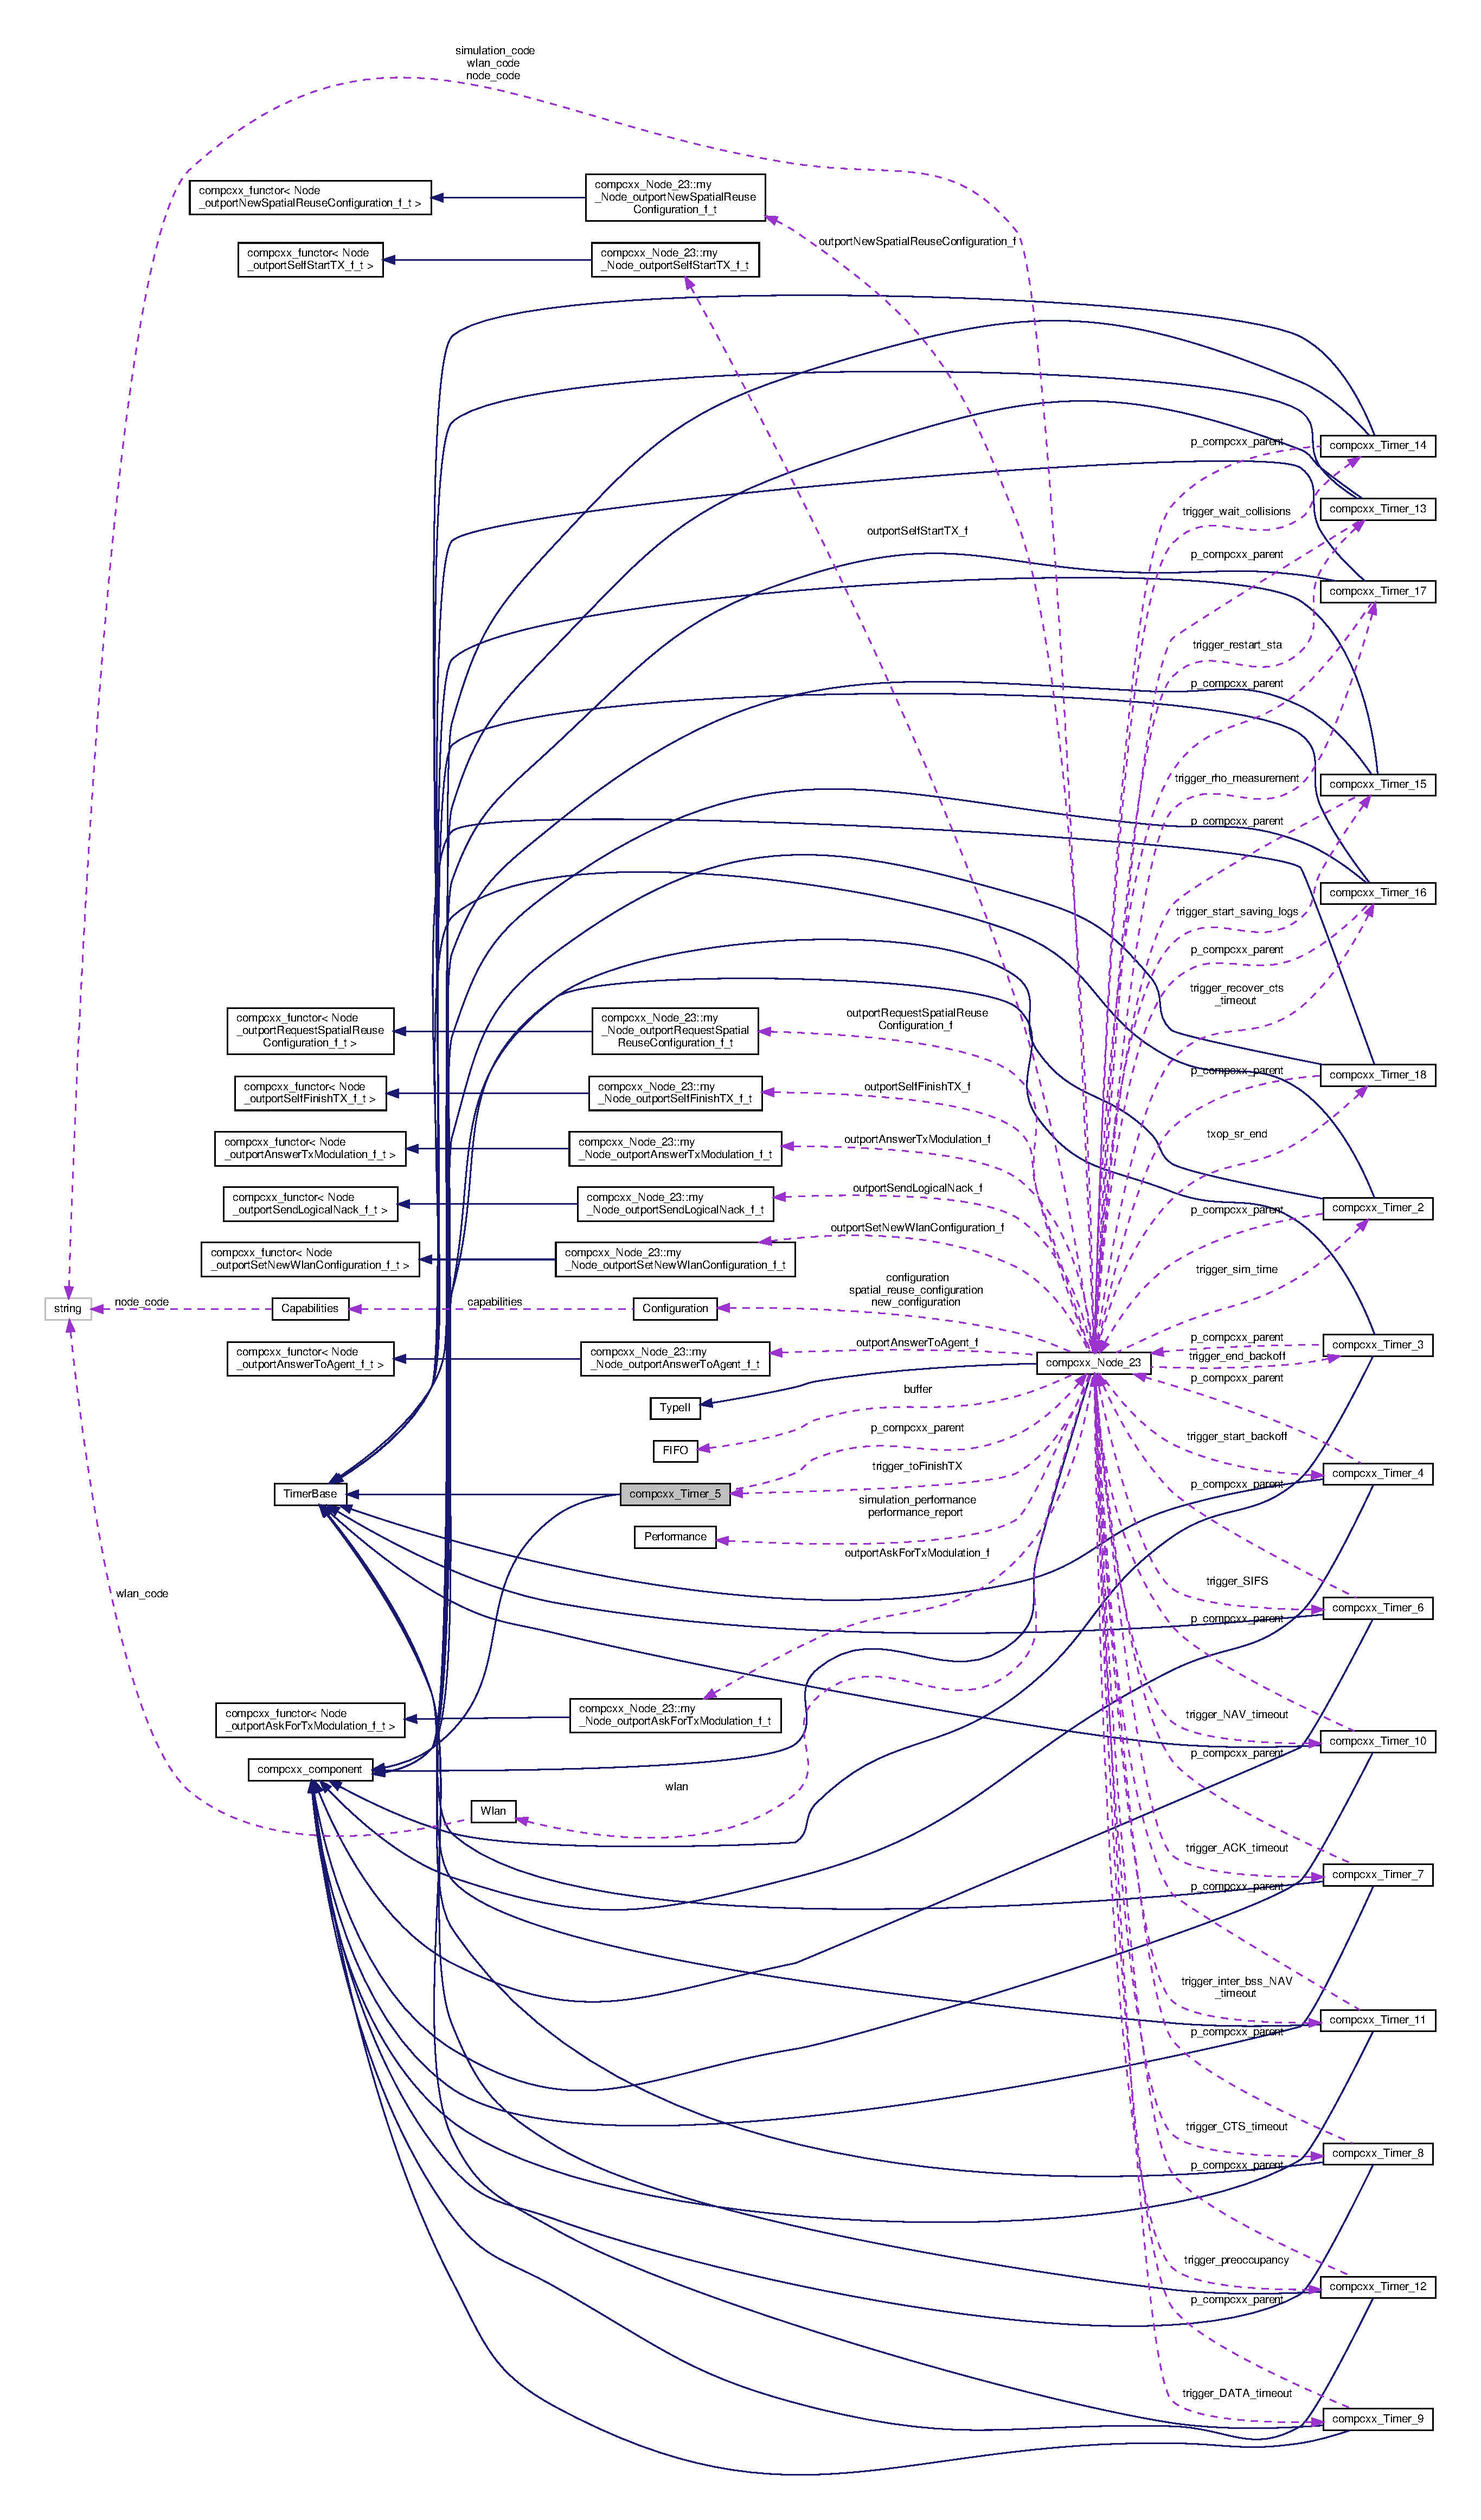
\includegraphics[height=550pt]{classcompcxx__Timer__5__coll__graph}
\end{center}
\end{figure}
\subsection*{Classes}
\begin{DoxyCompactItemize}
\item 
struct \hyperlink{structcompcxx__Timer__5_1_1event__t}{event\+\_\+t}
\end{DoxyCompactItemize}
\subsection*{Public Member Functions}
\begin{DoxyCompactItemize}
\item 
\mbox{\Hypertarget{classcompcxx__Timer__5_a23f81a12d761fe47382bc99d74a7e092}\label{classcompcxx__Timer__5_a23f81a12d761fe47382bc99d74a7e092}} 
void {\bfseries Set} (\hyperlink{classtrigger__t}{trigger\+\_\+t} const \&, double)
\item 
\mbox{\Hypertarget{classcompcxx__Timer__5_a9e9391302510b0aab11e81892c512b3d}\label{classcompcxx__Timer__5_a9e9391302510b0aab11e81892c512b3d}} 
void {\bfseries Set} (double)
\item 
\mbox{\Hypertarget{classcompcxx__Timer__5_a92d1fa976cd5630c76267484e89a94af}\label{classcompcxx__Timer__5_a92d1fa976cd5630c76267484e89a94af}} 
double {\bfseries Get\+Time} ()
\item 
\mbox{\Hypertarget{classcompcxx__Timer__5_af0cbb3cfc4237aa566c94b862ecf1684}\label{classcompcxx__Timer__5_af0cbb3cfc4237aa566c94b862ecf1684}} 
bool {\bfseries Active} ()
\item 
\mbox{\Hypertarget{classcompcxx__Timer__5_acbac5d5cefb85724ced45f896243335f}\label{classcompcxx__Timer__5_acbac5d5cefb85724ced45f896243335f}} 
\hyperlink{classtrigger__t}{trigger\+\_\+t} \& {\bfseries Get\+Data} ()
\item 
\mbox{\Hypertarget{classcompcxx__Timer__5_aa577b90551583b581a5cefc571fc8f4f}\label{classcompcxx__Timer__5_aa577b90551583b581a5cefc571fc8f4f}} 
void {\bfseries Set\+Data} (\hyperlink{classtrigger__t}{trigger\+\_\+t} const \&d)
\item 
\mbox{\Hypertarget{classcompcxx__Timer__5_af28bd1e54db76088d921a83750db1f4d}\label{classcompcxx__Timer__5_af28bd1e54db76088d921a83750db1f4d}} 
void {\bfseries Cancel} ()
\item 
\mbox{\Hypertarget{classcompcxx__Timer__5_ac1f9b15bf7f85ccb0f1e88f664e68426}\label{classcompcxx__Timer__5_ac1f9b15bf7f85ccb0f1e88f664e68426}} 
void {\bfseries activate} (\hyperlink{structCostEvent}{Cost\+Event} $\ast$)
\end{DoxyCompactItemize}
\subsection*{Public Attributes}
\begin{DoxyCompactItemize}
\item 
\mbox{\Hypertarget{classcompcxx__Timer__5_a6ed9578b0f3e92aec304480f39bbbbe2}\label{classcompcxx__Timer__5_a6ed9578b0f3e92aec304480f39bbbbe2}} 
\hyperlink{classcompcxx__Node__23}{compcxx\+\_\+\+Node\+\_\+23} $\ast$ {\bfseries p\+\_\+compcxx\+\_\+parent}
\end{DoxyCompactItemize}
\subsection*{Additional Inherited Members}


The documentation for this class was generated from the following file\+:\begin{DoxyCompactItemize}
\item 
Code/main/komondor\+\_\+main.\+cxx\end{DoxyCompactItemize}

\hypertarget{classcompcxx__Timer__6}{}\section{compcxx\+\_\+\+Timer\+\_\+6 Class Reference}
\label{classcompcxx__Timer__6}\index{compcxx\+\_\+\+Timer\+\_\+6@{compcxx\+\_\+\+Timer\+\_\+6}}


Inheritance diagram for compcxx\+\_\+\+Timer\+\_\+6\+:\nopagebreak
\begin{figure}[H]
\begin{center}
\leavevmode
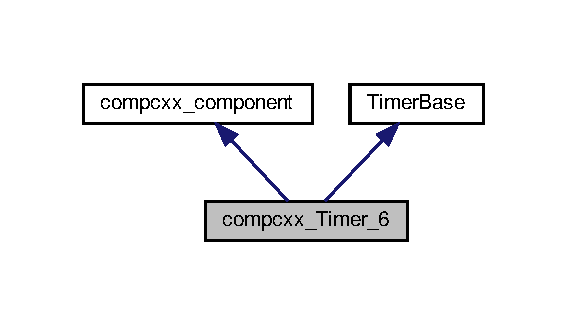
\includegraphics[width=272pt]{classcompcxx__Timer__6__inherit__graph}
\end{center}
\end{figure}


Collaboration diagram for compcxx\+\_\+\+Timer\+\_\+6\+:\nopagebreak
\begin{figure}[H]
\begin{center}
\leavevmode
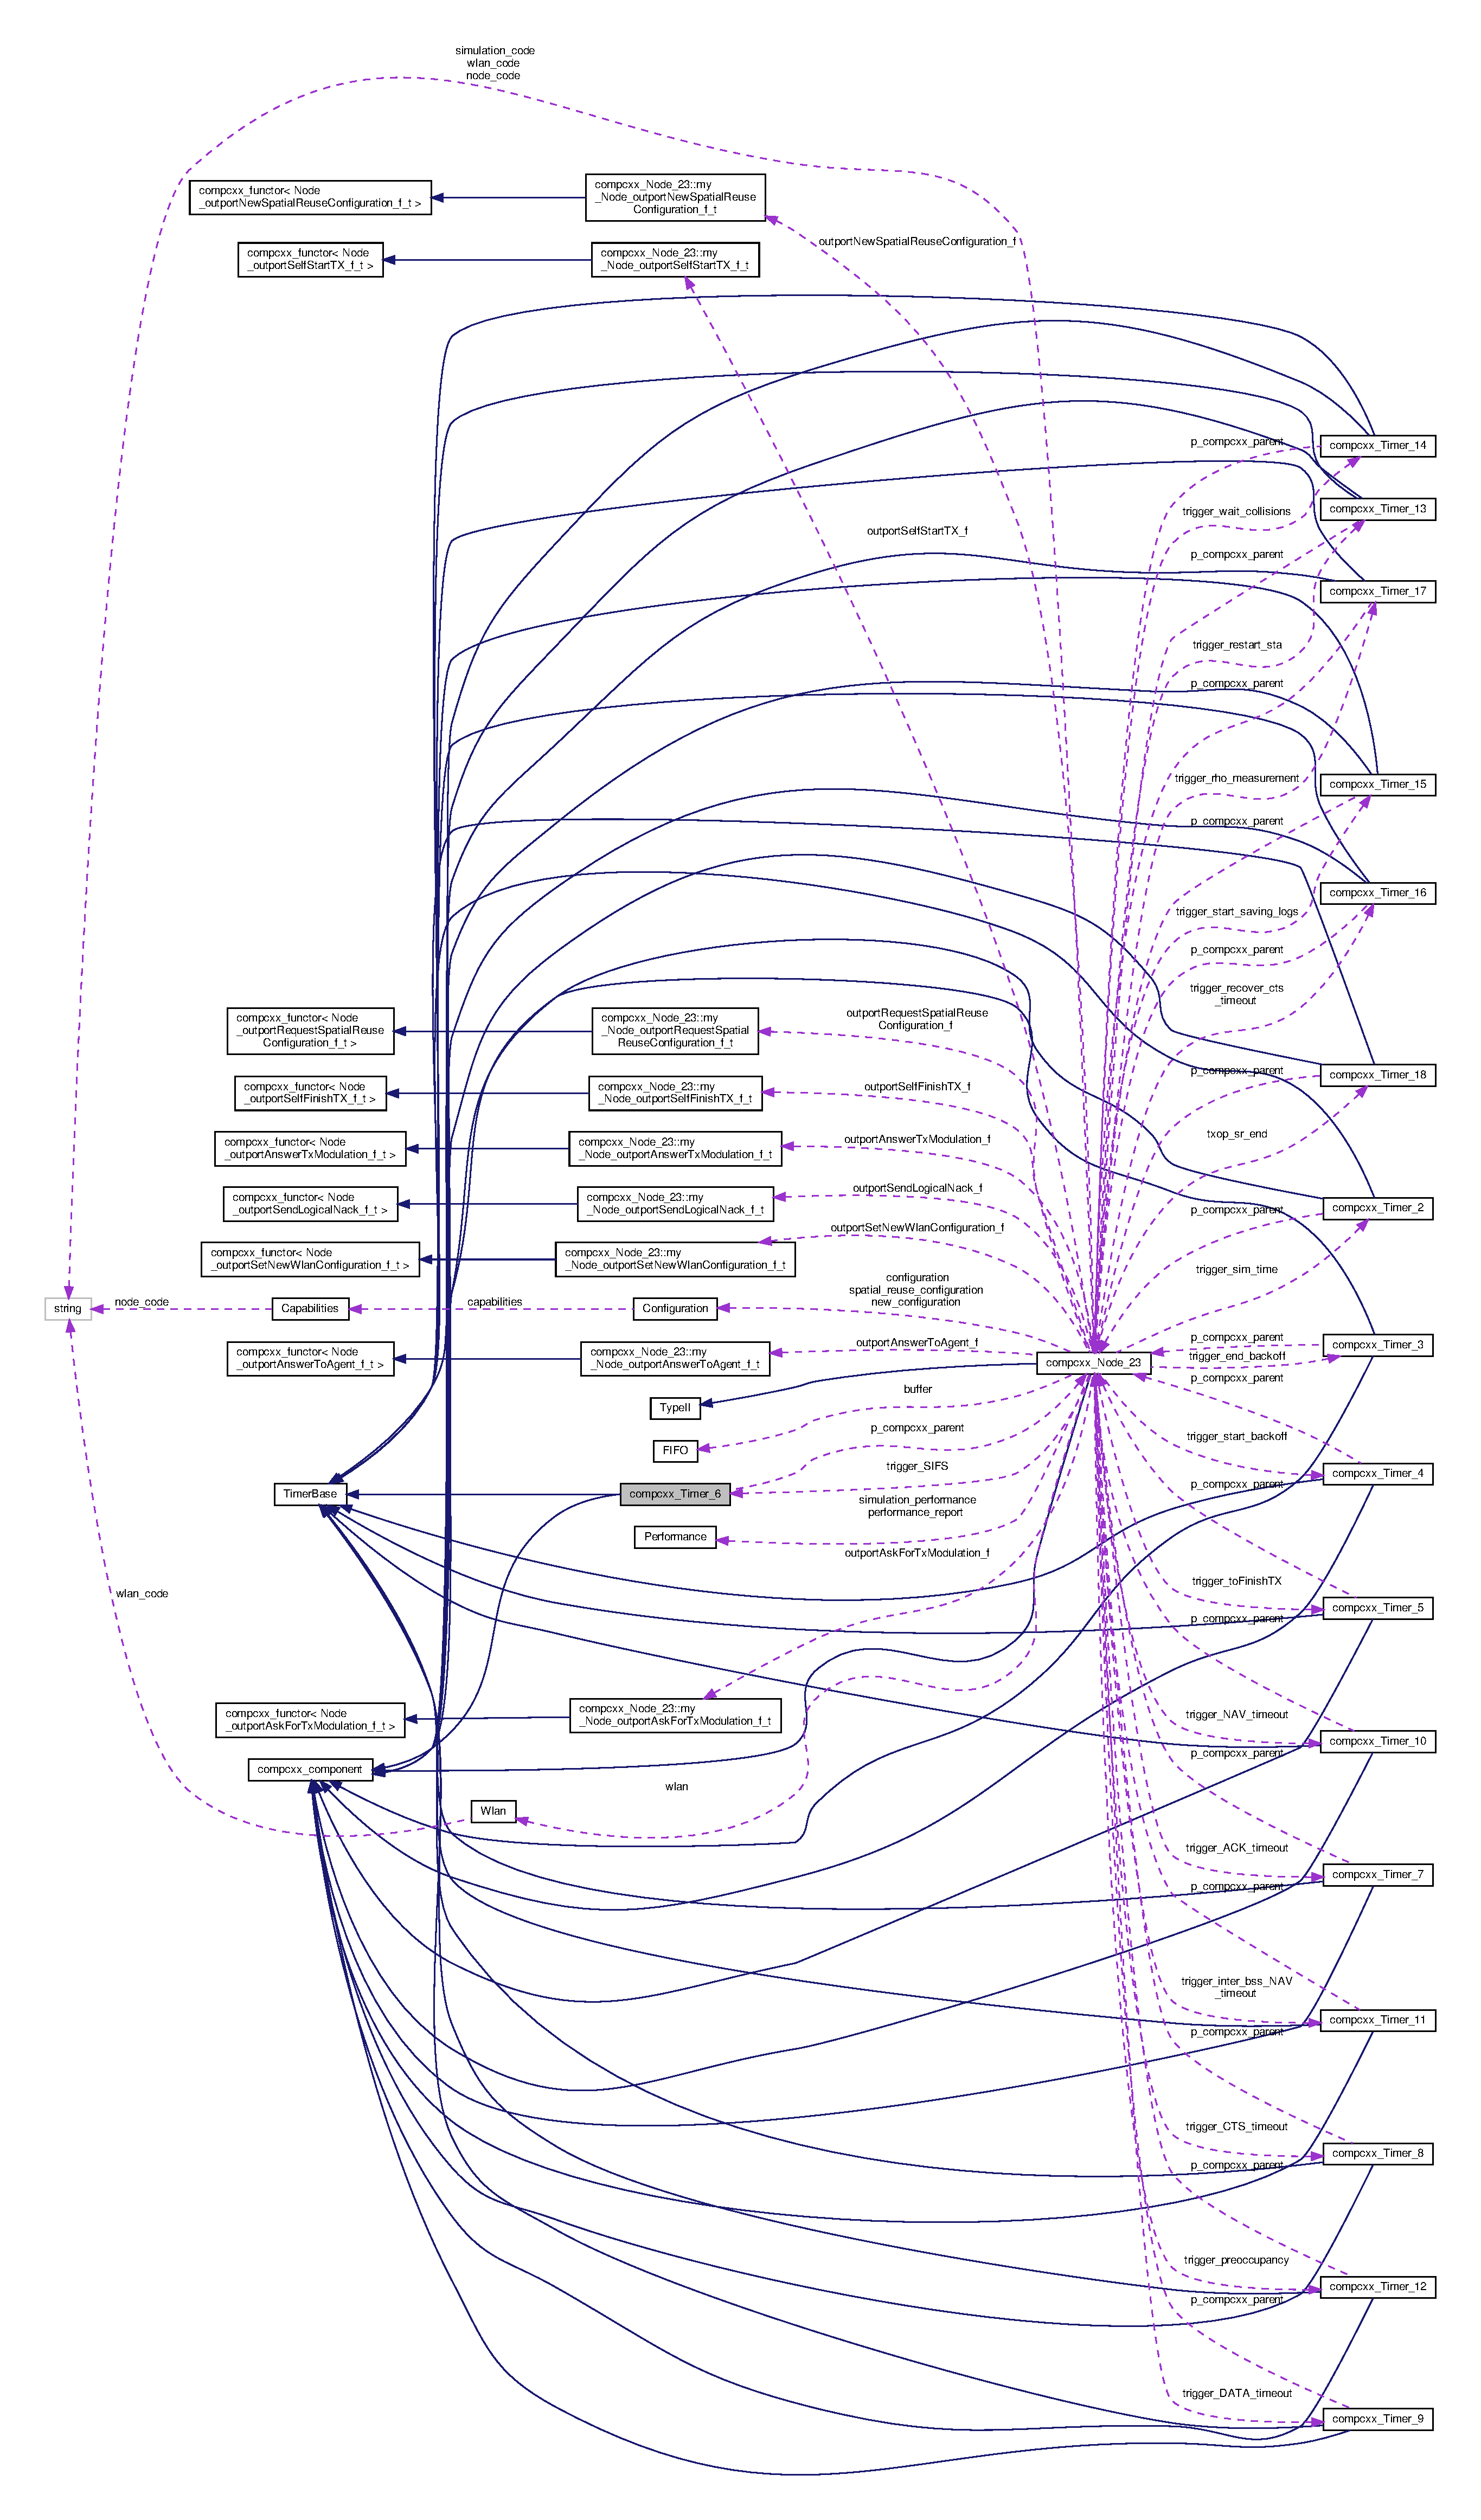
\includegraphics[height=550pt]{classcompcxx__Timer__6__coll__graph}
\end{center}
\end{figure}
\subsection*{Classes}
\begin{DoxyCompactItemize}
\item 
struct \hyperlink{structcompcxx__Timer__6_1_1event__t}{event\+\_\+t}
\end{DoxyCompactItemize}
\subsection*{Public Member Functions}
\begin{DoxyCompactItemize}
\item 
\mbox{\Hypertarget{classcompcxx__Timer__6_a9735459aea5eec06b5dd2f34621cf408}\label{classcompcxx__Timer__6_a9735459aea5eec06b5dd2f34621cf408}} 
void {\bfseries Set} (\hyperlink{classtrigger__t}{trigger\+\_\+t} const \&, double)
\item 
\mbox{\Hypertarget{classcompcxx__Timer__6_a79e592f7a73c6d61313b866c9dc5641a}\label{classcompcxx__Timer__6_a79e592f7a73c6d61313b866c9dc5641a}} 
void {\bfseries Set} (double)
\item 
\mbox{\Hypertarget{classcompcxx__Timer__6_a1a0145ade61dff19fb076dd5df765567}\label{classcompcxx__Timer__6_a1a0145ade61dff19fb076dd5df765567}} 
double {\bfseries Get\+Time} ()
\item 
\mbox{\Hypertarget{classcompcxx__Timer__6_ab4baec2665ce86a6133af343284ff29b}\label{classcompcxx__Timer__6_ab4baec2665ce86a6133af343284ff29b}} 
bool {\bfseries Active} ()
\item 
\mbox{\Hypertarget{classcompcxx__Timer__6_a8afc494d405de76f36794d1fd126db11}\label{classcompcxx__Timer__6_a8afc494d405de76f36794d1fd126db11}} 
\hyperlink{classtrigger__t}{trigger\+\_\+t} \& {\bfseries Get\+Data} ()
\item 
\mbox{\Hypertarget{classcompcxx__Timer__6_a080bc12841dee0ce3dfaffe24ac76452}\label{classcompcxx__Timer__6_a080bc12841dee0ce3dfaffe24ac76452}} 
void {\bfseries Set\+Data} (\hyperlink{classtrigger__t}{trigger\+\_\+t} const \&d)
\item 
\mbox{\Hypertarget{classcompcxx__Timer__6_ad2155c8e9caaf527530a86cad52f1721}\label{classcompcxx__Timer__6_ad2155c8e9caaf527530a86cad52f1721}} 
void {\bfseries Cancel} ()
\item 
\mbox{\Hypertarget{classcompcxx__Timer__6_ad2d8b0d5d0a54a050f83ed39819fb763}\label{classcompcxx__Timer__6_ad2d8b0d5d0a54a050f83ed39819fb763}} 
void {\bfseries activate} (\hyperlink{structCostEvent}{Cost\+Event} $\ast$)
\end{DoxyCompactItemize}
\subsection*{Public Attributes}
\begin{DoxyCompactItemize}
\item 
\mbox{\Hypertarget{classcompcxx__Timer__6_abd962180b00c4b687e502cac46346b6f}\label{classcompcxx__Timer__6_abd962180b00c4b687e502cac46346b6f}} 
\hyperlink{classcompcxx__Node__23}{compcxx\+\_\+\+Node\+\_\+23} $\ast$ {\bfseries p\+\_\+compcxx\+\_\+parent}
\end{DoxyCompactItemize}
\subsection*{Additional Inherited Members}


The documentation for this class was generated from the following file\+:\begin{DoxyCompactItemize}
\item 
Code/main/komondor\+\_\+main.\+cxx\end{DoxyCompactItemize}

\hypertarget{classcompcxx__Timer__7}{}\section{compcxx\+\_\+\+Timer\+\_\+7 Class Reference}
\label{classcompcxx__Timer__7}\index{compcxx\+\_\+\+Timer\+\_\+7@{compcxx\+\_\+\+Timer\+\_\+7}}


Inheritance diagram for compcxx\+\_\+\+Timer\+\_\+7\+:\nopagebreak
\begin{figure}[H]
\begin{center}
\leavevmode
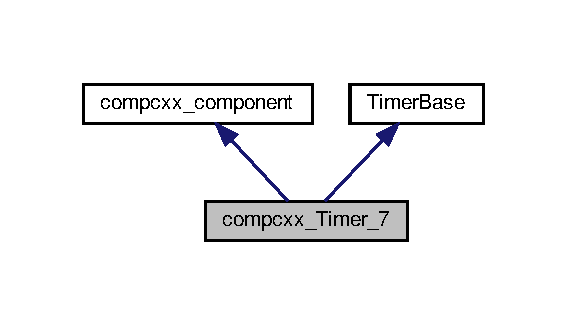
\includegraphics[width=272pt]{classcompcxx__Timer__7__inherit__graph}
\end{center}
\end{figure}


Collaboration diagram for compcxx\+\_\+\+Timer\+\_\+7\+:\nopagebreak
\begin{figure}[H]
\begin{center}
\leavevmode
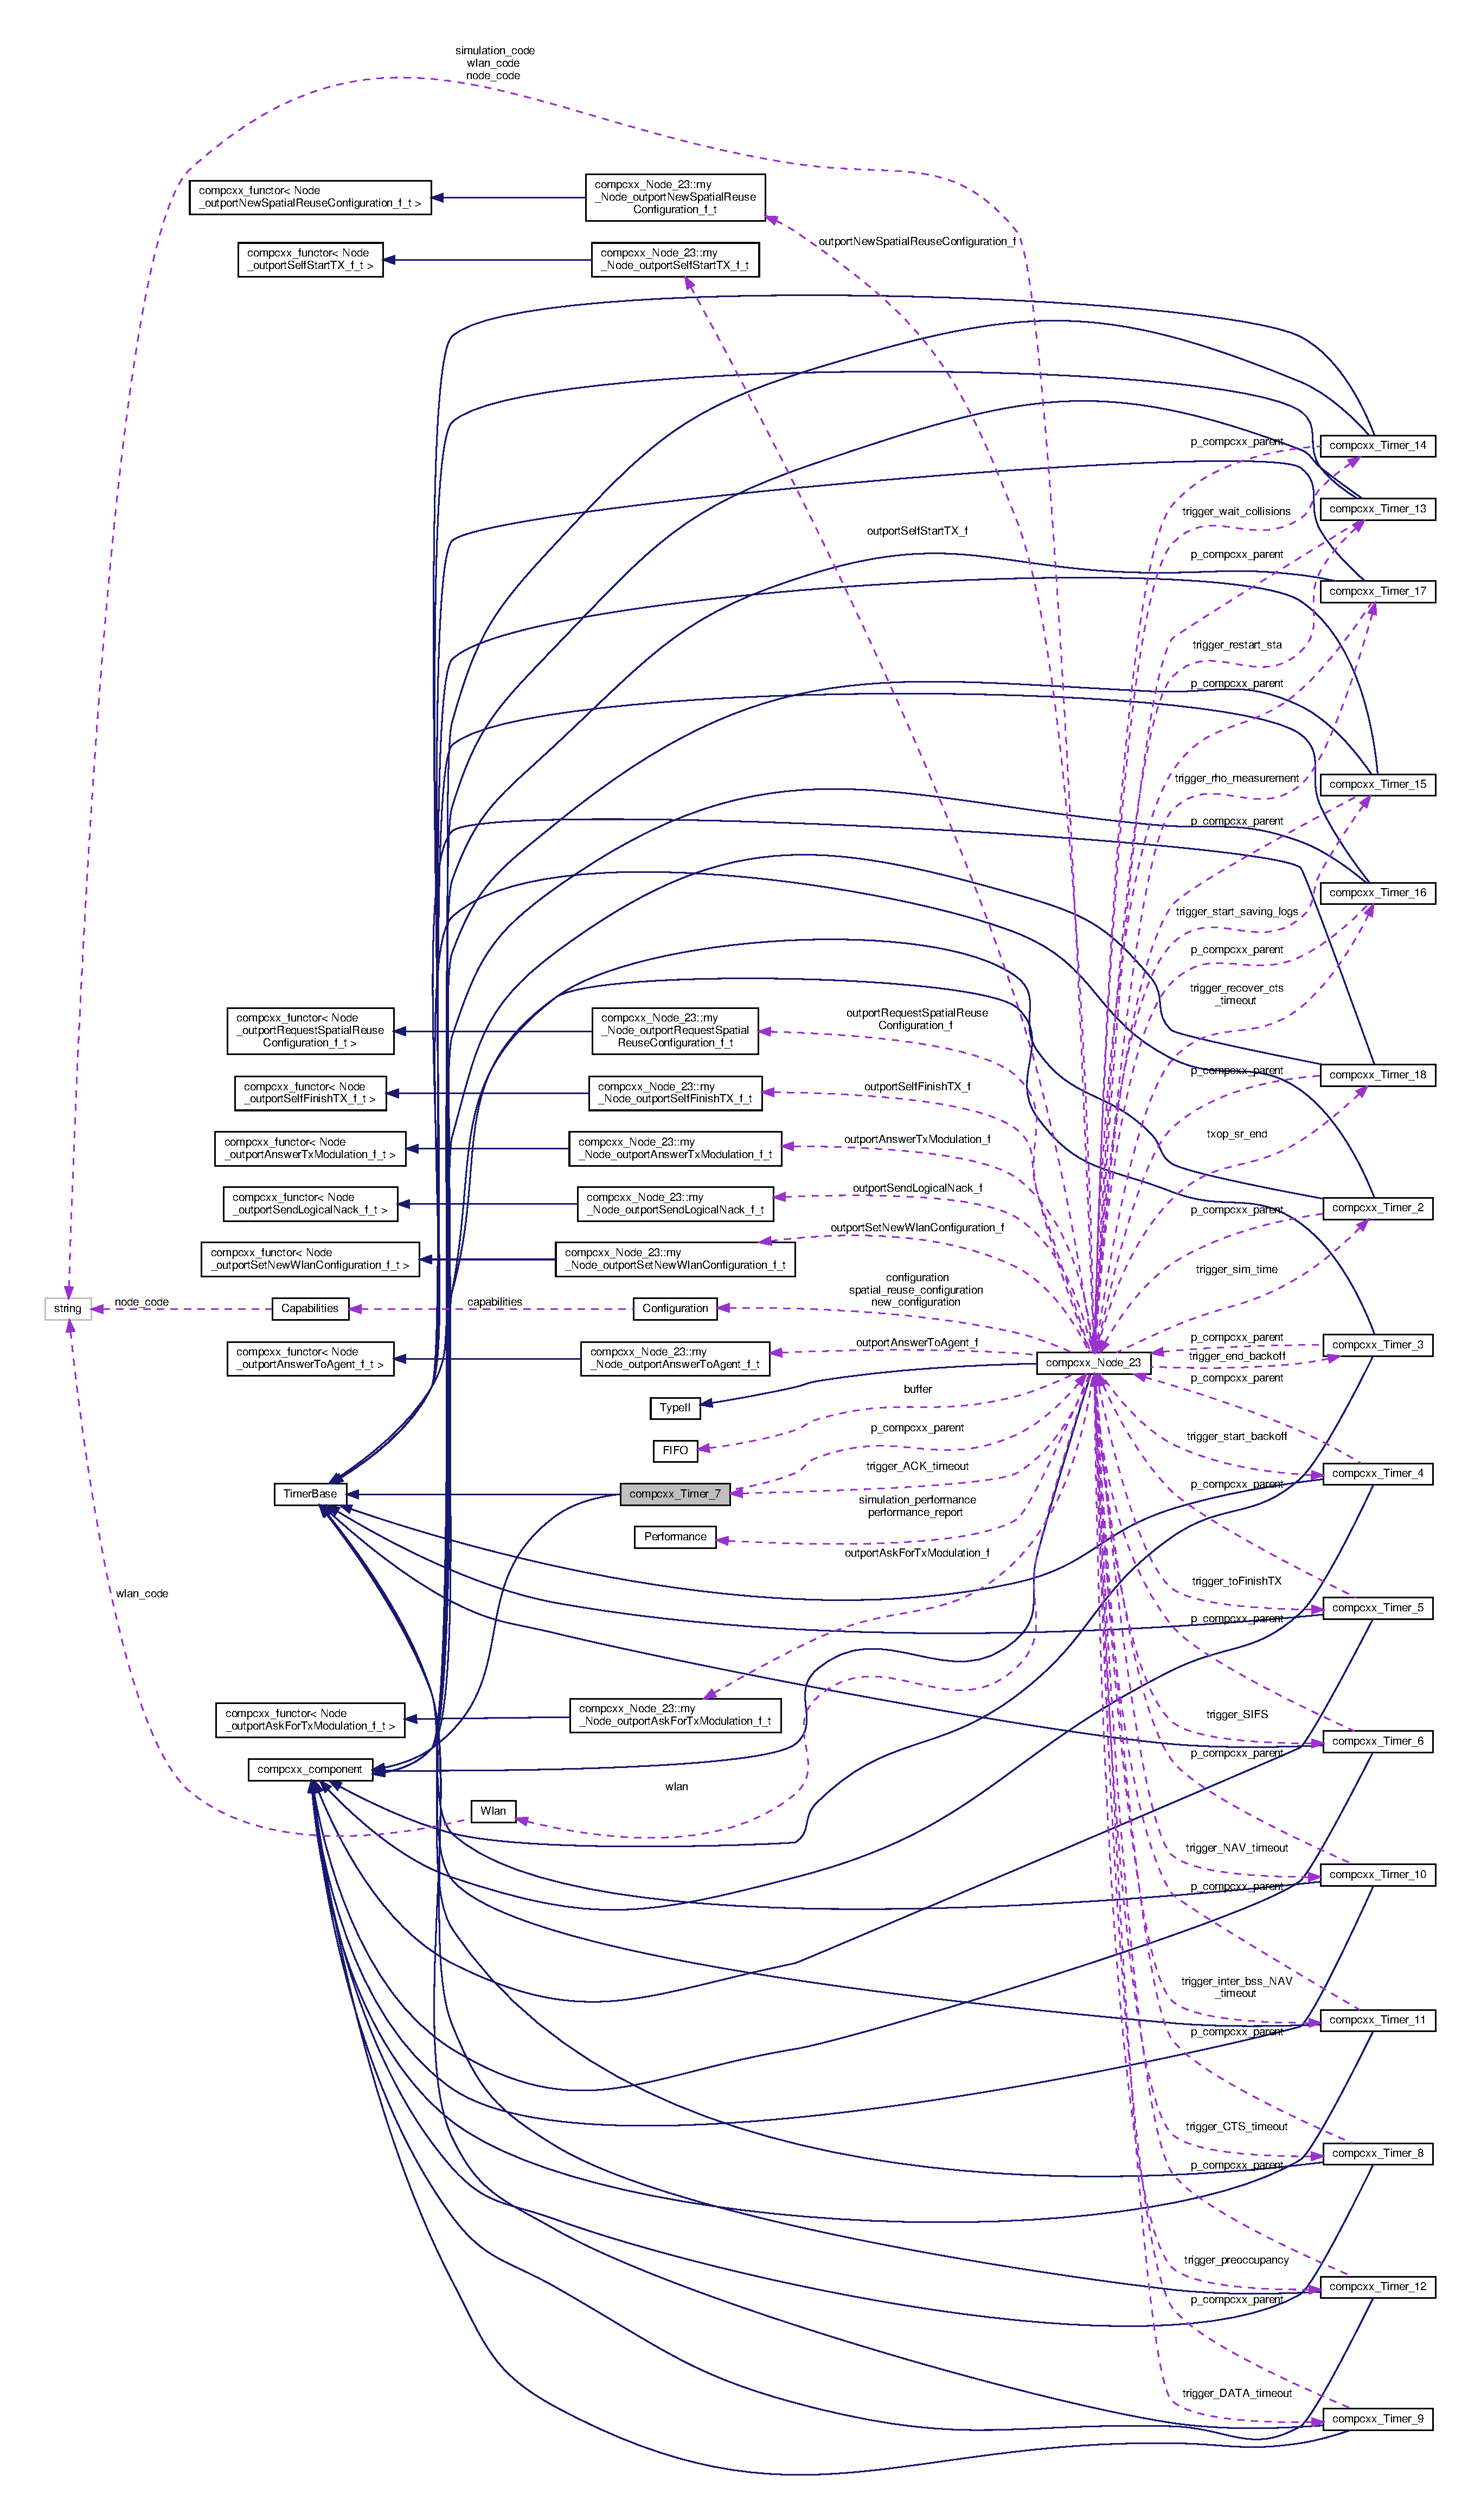
\includegraphics[height=550pt]{classcompcxx__Timer__7__coll__graph}
\end{center}
\end{figure}
\subsection*{Classes}
\begin{DoxyCompactItemize}
\item 
struct \hyperlink{structcompcxx__Timer__7_1_1event__t}{event\+\_\+t}
\end{DoxyCompactItemize}
\subsection*{Public Member Functions}
\begin{DoxyCompactItemize}
\item 
\mbox{\Hypertarget{classcompcxx__Timer__7_ad59728217fda9ea9daa578ce862c8bb4}\label{classcompcxx__Timer__7_ad59728217fda9ea9daa578ce862c8bb4}} 
void {\bfseries Set} (\hyperlink{classtrigger__t}{trigger\+\_\+t} const \&, double)
\item 
\mbox{\Hypertarget{classcompcxx__Timer__7_a74b0a0c43273692bc4f7d32d75954a6f}\label{classcompcxx__Timer__7_a74b0a0c43273692bc4f7d32d75954a6f}} 
void {\bfseries Set} (double)
\item 
\mbox{\Hypertarget{classcompcxx__Timer__7_a20987f2e07807729b30434d61a943c34}\label{classcompcxx__Timer__7_a20987f2e07807729b30434d61a943c34}} 
double {\bfseries Get\+Time} ()
\item 
\mbox{\Hypertarget{classcompcxx__Timer__7_aa71af403064a2874d7b77d9146594385}\label{classcompcxx__Timer__7_aa71af403064a2874d7b77d9146594385}} 
bool {\bfseries Active} ()
\item 
\mbox{\Hypertarget{classcompcxx__Timer__7_a2535eed0cce55fd487148750932ccc3f}\label{classcompcxx__Timer__7_a2535eed0cce55fd487148750932ccc3f}} 
\hyperlink{classtrigger__t}{trigger\+\_\+t} \& {\bfseries Get\+Data} ()
\item 
\mbox{\Hypertarget{classcompcxx__Timer__7_a5b2cea4ad04e661c7265f9261f70282c}\label{classcompcxx__Timer__7_a5b2cea4ad04e661c7265f9261f70282c}} 
void {\bfseries Set\+Data} (\hyperlink{classtrigger__t}{trigger\+\_\+t} const \&d)
\item 
\mbox{\Hypertarget{classcompcxx__Timer__7_a1dced48b7fe170013c34064a5dc0de5d}\label{classcompcxx__Timer__7_a1dced48b7fe170013c34064a5dc0de5d}} 
void {\bfseries Cancel} ()
\item 
\mbox{\Hypertarget{classcompcxx__Timer__7_a0f4f300c828895ca420e9119ffd565bc}\label{classcompcxx__Timer__7_a0f4f300c828895ca420e9119ffd565bc}} 
void {\bfseries activate} (\hyperlink{structCostEvent}{Cost\+Event} $\ast$)
\end{DoxyCompactItemize}
\subsection*{Public Attributes}
\begin{DoxyCompactItemize}
\item 
\mbox{\Hypertarget{classcompcxx__Timer__7_ad1e43ee729caafc83962306fdf9db38b}\label{classcompcxx__Timer__7_ad1e43ee729caafc83962306fdf9db38b}} 
\hyperlink{classcompcxx__Node__23}{compcxx\+\_\+\+Node\+\_\+23} $\ast$ {\bfseries p\+\_\+compcxx\+\_\+parent}
\end{DoxyCompactItemize}
\subsection*{Additional Inherited Members}


The documentation for this class was generated from the following file\+:\begin{DoxyCompactItemize}
\item 
Code/main/komondor\+\_\+main.\+cxx\end{DoxyCompactItemize}

\hypertarget{classcompcxx__Timer__8}{}\section{compcxx\+\_\+\+Timer\+\_\+8 Class Reference}
\label{classcompcxx__Timer__8}\index{compcxx\+\_\+\+Timer\+\_\+8@{compcxx\+\_\+\+Timer\+\_\+8}}


Inheritance diagram for compcxx\+\_\+\+Timer\+\_\+8\+:\nopagebreak
\begin{figure}[H]
\begin{center}
\leavevmode
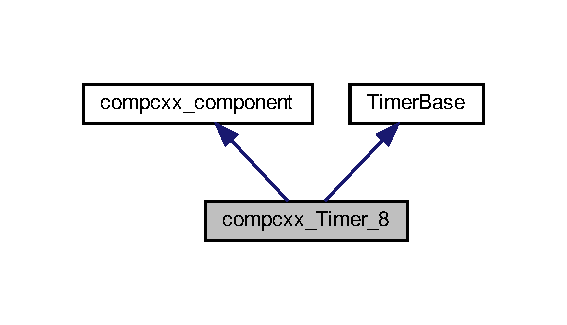
\includegraphics[width=272pt]{classcompcxx__Timer__8__inherit__graph}
\end{center}
\end{figure}


Collaboration diagram for compcxx\+\_\+\+Timer\+\_\+8\+:\nopagebreak
\begin{figure}[H]
\begin{center}
\leavevmode
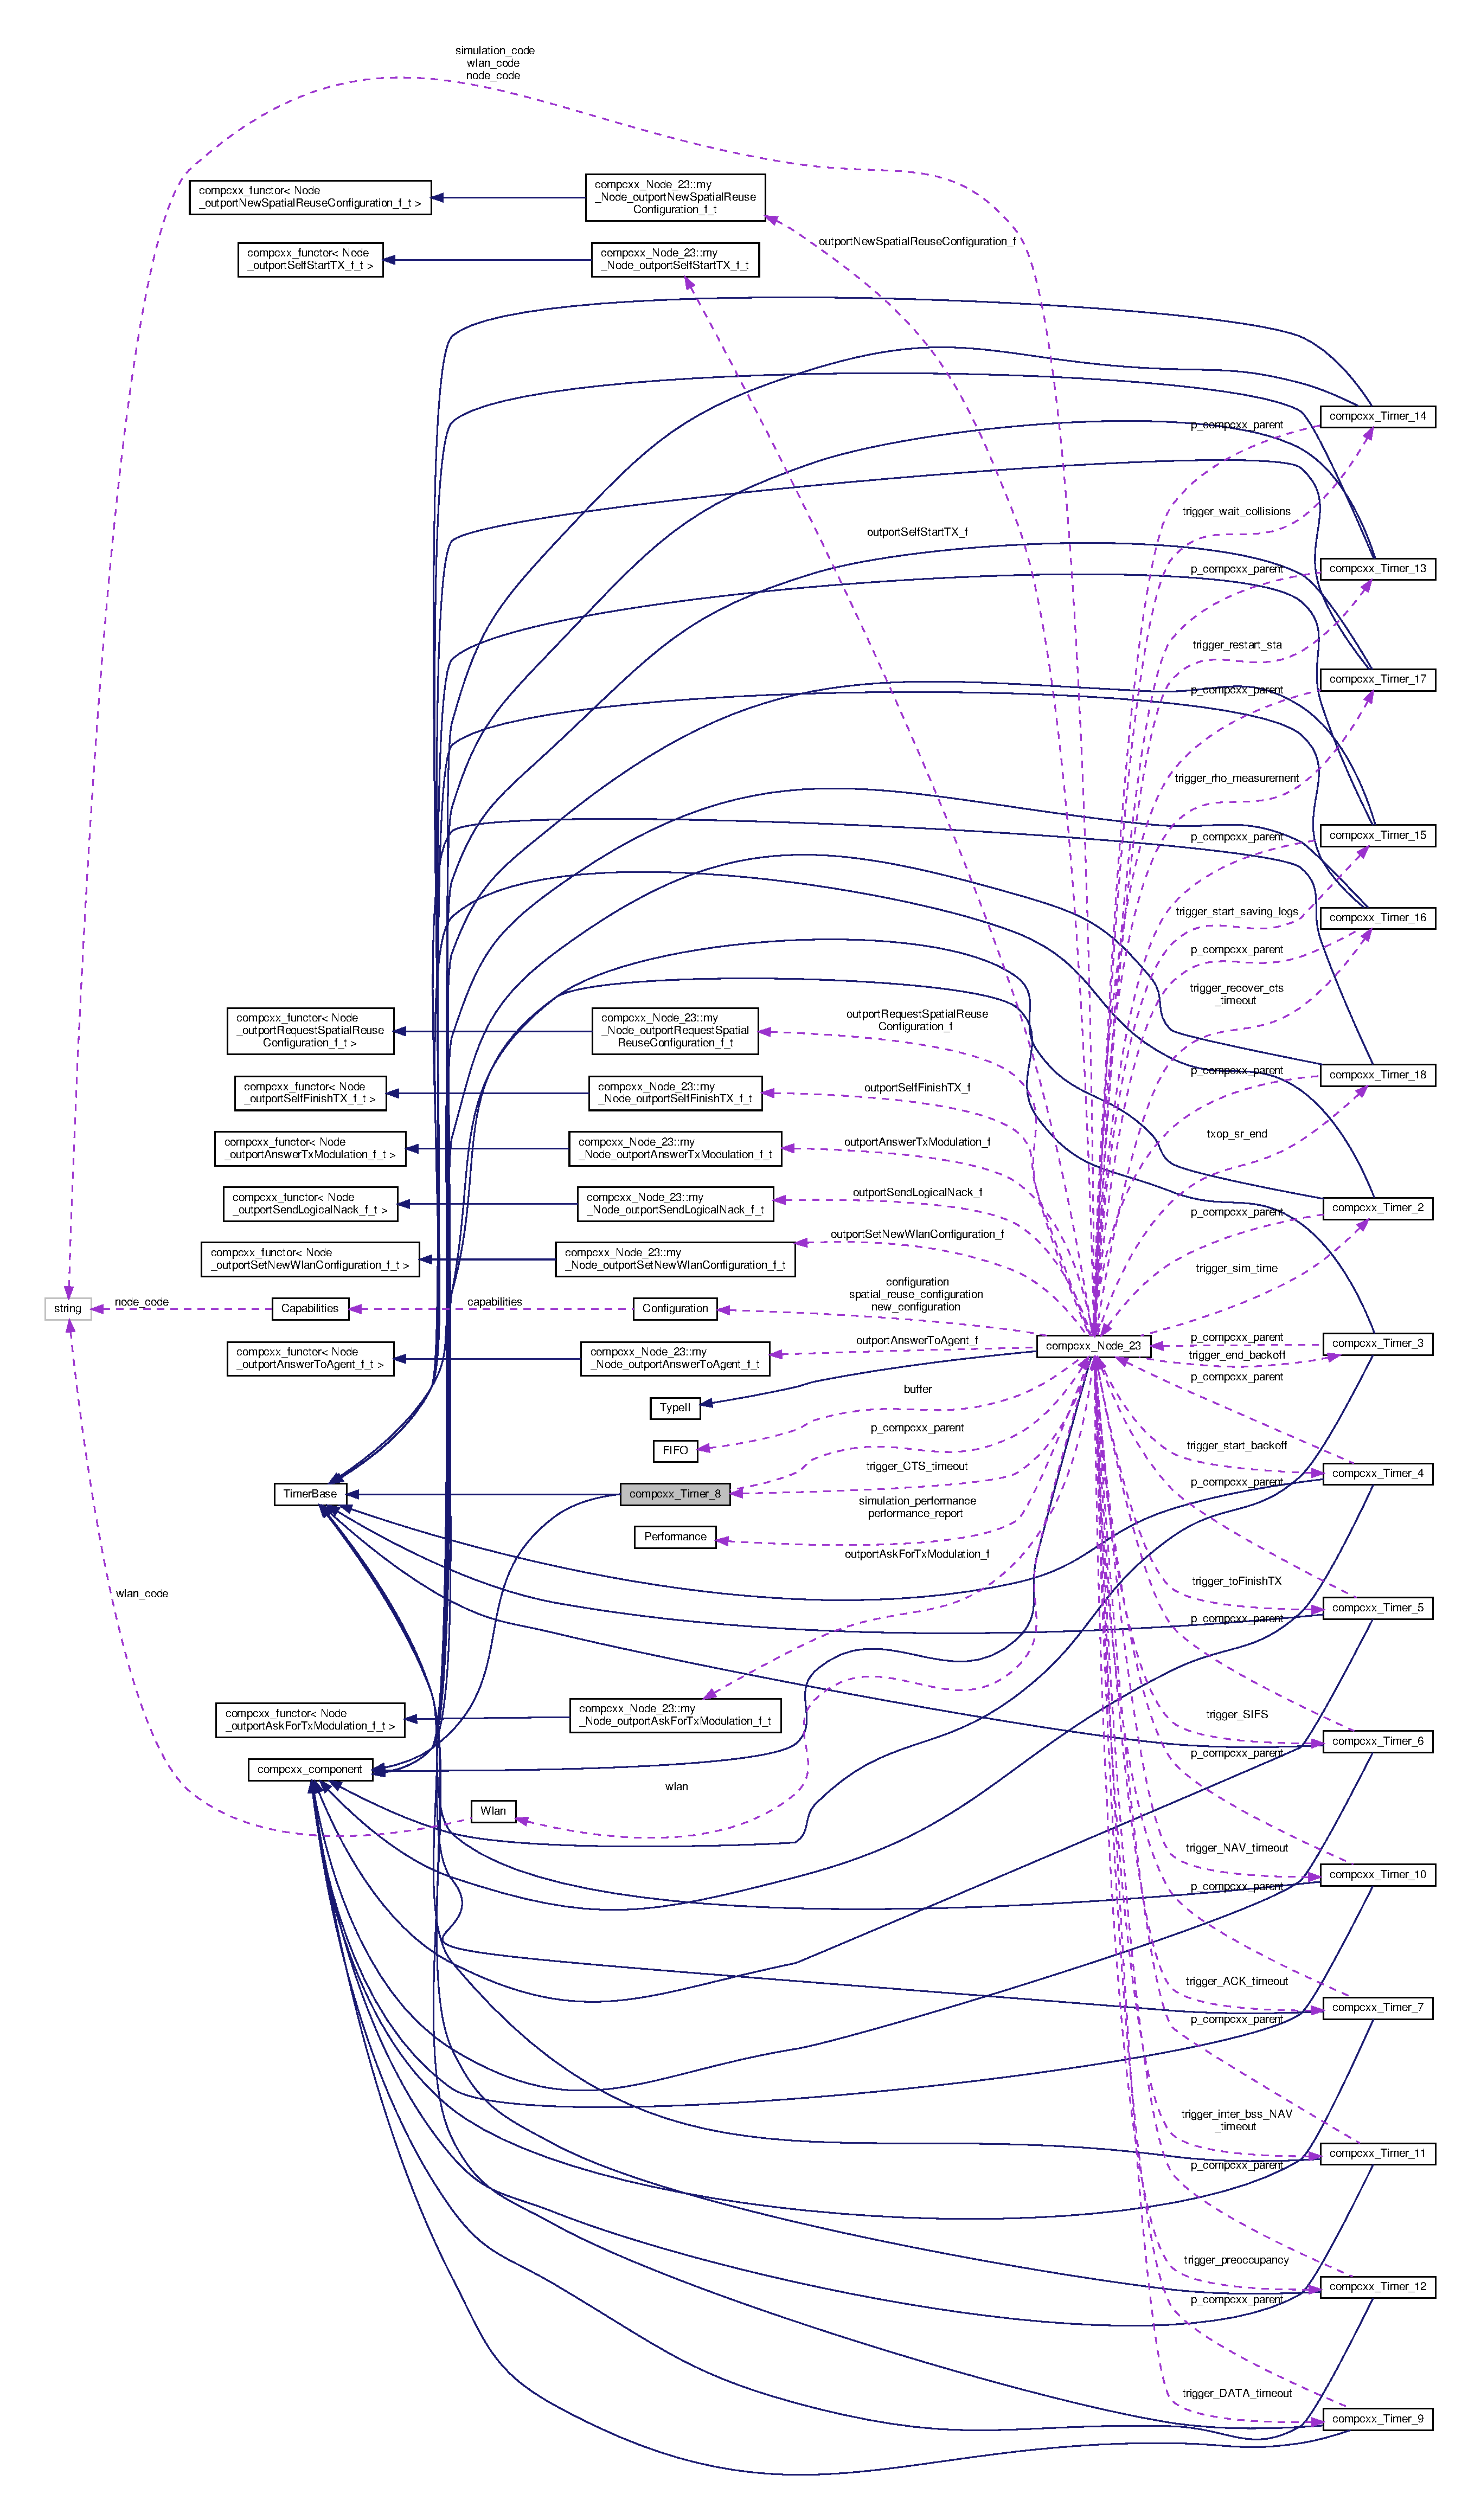
\includegraphics[height=550pt]{classcompcxx__Timer__8__coll__graph}
\end{center}
\end{figure}
\subsection*{Classes}
\begin{DoxyCompactItemize}
\item 
struct \hyperlink{structcompcxx__Timer__8_1_1event__t}{event\+\_\+t}
\end{DoxyCompactItemize}
\subsection*{Public Member Functions}
\begin{DoxyCompactItemize}
\item 
\mbox{\Hypertarget{classcompcxx__Timer__8_ad88e11cfcb34c9d0a4a66a021bc98b91}\label{classcompcxx__Timer__8_ad88e11cfcb34c9d0a4a66a021bc98b91}} 
void {\bfseries Set} (\hyperlink{classtrigger__t}{trigger\+\_\+t} const \&, double)
\item 
\mbox{\Hypertarget{classcompcxx__Timer__8_a1335efa532e6510353bfe4decc74fc66}\label{classcompcxx__Timer__8_a1335efa532e6510353bfe4decc74fc66}} 
void {\bfseries Set} (double)
\item 
\mbox{\Hypertarget{classcompcxx__Timer__8_a74fff42e8bd8eb776e5f8f221e0ce3f0}\label{classcompcxx__Timer__8_a74fff42e8bd8eb776e5f8f221e0ce3f0}} 
double {\bfseries Get\+Time} ()
\item 
\mbox{\Hypertarget{classcompcxx__Timer__8_a6d6a2e2df684e62db401fe7b250c1fd1}\label{classcompcxx__Timer__8_a6d6a2e2df684e62db401fe7b250c1fd1}} 
bool {\bfseries Active} ()
\item 
\mbox{\Hypertarget{classcompcxx__Timer__8_aca1afd4692a350ef15ea6471700ccccb}\label{classcompcxx__Timer__8_aca1afd4692a350ef15ea6471700ccccb}} 
\hyperlink{classtrigger__t}{trigger\+\_\+t} \& {\bfseries Get\+Data} ()
\item 
\mbox{\Hypertarget{classcompcxx__Timer__8_a73eccaa7bf685952be9fa213ede63684}\label{classcompcxx__Timer__8_a73eccaa7bf685952be9fa213ede63684}} 
void {\bfseries Set\+Data} (\hyperlink{classtrigger__t}{trigger\+\_\+t} const \&d)
\item 
\mbox{\Hypertarget{classcompcxx__Timer__8_a0a55ce254420f1140c74162cae368797}\label{classcompcxx__Timer__8_a0a55ce254420f1140c74162cae368797}} 
void {\bfseries Cancel} ()
\item 
\mbox{\Hypertarget{classcompcxx__Timer__8_a6324c18b710bf7316af086e33a88a8f3}\label{classcompcxx__Timer__8_a6324c18b710bf7316af086e33a88a8f3}} 
void {\bfseries activate} (\hyperlink{structCostEvent}{Cost\+Event} $\ast$)
\end{DoxyCompactItemize}
\subsection*{Public Attributes}
\begin{DoxyCompactItemize}
\item 
\mbox{\Hypertarget{classcompcxx__Timer__8_a106e163f22842216b1047ade6badc47b}\label{classcompcxx__Timer__8_a106e163f22842216b1047ade6badc47b}} 
\hyperlink{classcompcxx__Node__23}{compcxx\+\_\+\+Node\+\_\+23} $\ast$ {\bfseries p\+\_\+compcxx\+\_\+parent}
\end{DoxyCompactItemize}
\subsection*{Additional Inherited Members}


The documentation for this class was generated from the following file\+:\begin{DoxyCompactItemize}
\item 
Code/main/komondor\+\_\+main.\+cxx\end{DoxyCompactItemize}

\hypertarget{classcompcxx__Timer__9}{}\section{compcxx\+\_\+\+Timer\+\_\+9 Class Reference}
\label{classcompcxx__Timer__9}\index{compcxx\+\_\+\+Timer\+\_\+9@{compcxx\+\_\+\+Timer\+\_\+9}}


Inheritance diagram for compcxx\+\_\+\+Timer\+\_\+9\+:\nopagebreak
\begin{figure}[H]
\begin{center}
\leavevmode
\includegraphics[width=272pt]{classcompcxx__Timer__9__inherit__graph}
\end{center}
\end{figure}


Collaboration diagram for compcxx\+\_\+\+Timer\+\_\+9\+:\nopagebreak
\begin{figure}[H]
\begin{center}
\leavevmode
\includegraphics[height=550pt]{classcompcxx__Timer__9__coll__graph}
\end{center}
\end{figure}
\subsection*{Classes}
\begin{DoxyCompactItemize}
\item 
struct \hyperlink{structcompcxx__Timer__9_1_1event__t}{event\+\_\+t}
\end{DoxyCompactItemize}
\subsection*{Public Member Functions}
\begin{DoxyCompactItemize}
\item 
\mbox{\Hypertarget{classcompcxx__Timer__9_a64d41724034ebf786608cf02d6b4729f}\label{classcompcxx__Timer__9_a64d41724034ebf786608cf02d6b4729f}} 
void {\bfseries Set} (\hyperlink{classtrigger__t}{trigger\+\_\+t} const \&, double)
\item 
\mbox{\Hypertarget{classcompcxx__Timer__9_a691cdecc005e6c690bbc2193482775f3}\label{classcompcxx__Timer__9_a691cdecc005e6c690bbc2193482775f3}} 
void {\bfseries Set} (double)
\item 
\mbox{\Hypertarget{classcompcxx__Timer__9_ab3c9f0c524d1d44903e65a663a97a50e}\label{classcompcxx__Timer__9_ab3c9f0c524d1d44903e65a663a97a50e}} 
double {\bfseries Get\+Time} ()
\item 
\mbox{\Hypertarget{classcompcxx__Timer__9_aa96d058ff975ecbc3a03b7c9a7815a58}\label{classcompcxx__Timer__9_aa96d058ff975ecbc3a03b7c9a7815a58}} 
bool {\bfseries Active} ()
\item 
\mbox{\Hypertarget{classcompcxx__Timer__9_a430810e9e2927cf7aee9adab06bb29d6}\label{classcompcxx__Timer__9_a430810e9e2927cf7aee9adab06bb29d6}} 
\hyperlink{classtrigger__t}{trigger\+\_\+t} \& {\bfseries Get\+Data} ()
\item 
\mbox{\Hypertarget{classcompcxx__Timer__9_a51071fb918ae2e0ee305299421bb5d14}\label{classcompcxx__Timer__9_a51071fb918ae2e0ee305299421bb5d14}} 
void {\bfseries Set\+Data} (\hyperlink{classtrigger__t}{trigger\+\_\+t} const \&d)
\item 
\mbox{\Hypertarget{classcompcxx__Timer__9_a788c7b5323c0fcb2d81beab06f9ca0b7}\label{classcompcxx__Timer__9_a788c7b5323c0fcb2d81beab06f9ca0b7}} 
void {\bfseries Cancel} ()
\item 
\mbox{\Hypertarget{classcompcxx__Timer__9_a45801dc6fe888eb80fb7ff3d05967b89}\label{classcompcxx__Timer__9_a45801dc6fe888eb80fb7ff3d05967b89}} 
void {\bfseries activate} (\hyperlink{structCostEvent}{Cost\+Event} $\ast$)
\end{DoxyCompactItemize}
\subsection*{Public Attributes}
\begin{DoxyCompactItemize}
\item 
\mbox{\Hypertarget{classcompcxx__Timer__9_ae1ba3d3a9d881cb968a9bdb70240024f}\label{classcompcxx__Timer__9_ae1ba3d3a9d881cb968a9bdb70240024f}} 
\hyperlink{classcompcxx__Node__23}{compcxx\+\_\+\+Node\+\_\+23} $\ast$ {\bfseries p\+\_\+compcxx\+\_\+parent}
\end{DoxyCompactItemize}
\subsection*{Additional Inherited Members}


The documentation for this class was generated from the following file\+:\begin{DoxyCompactItemize}
\item 
Code/main/komondor\+\_\+main.\+cxx\end{DoxyCompactItemize}

\hypertarget{classcompcxx__TrafficGenerator__24}{}\section{compcxx\+\_\+\+Traffic\+Generator\+\_\+24 Class Reference}
\label{classcompcxx__TrafficGenerator__24}\index{compcxx\+\_\+\+Traffic\+Generator\+\_\+24@{compcxx\+\_\+\+Traffic\+Generator\+\_\+24}}


Inheritance diagram for compcxx\+\_\+\+Traffic\+Generator\+\_\+24\+:\nopagebreak
\begin{figure}[H]
\begin{center}
\leavevmode
\includegraphics[width=256pt]{classcompcxx__TrafficGenerator__24__inherit__graph}
\end{center}
\end{figure}


Collaboration diagram for compcxx\+\_\+\+Traffic\+Generator\+\_\+24\+:\nopagebreak
\begin{figure}[H]
\begin{center}
\leavevmode
\includegraphics[width=350pt]{classcompcxx__TrafficGenerator__24__coll__graph}
\end{center}
\end{figure}
\subsection*{Classes}
\begin{DoxyCompactItemize}
\item 
class \hyperlink{classcompcxx__TrafficGenerator__24_1_1my__TrafficGenerator__outportNewPacketGenerated__f__t}{my\+\_\+\+Traffic\+Generator\+\_\+outport\+New\+Packet\+Generated\+\_\+f\+\_\+t}
\end{DoxyCompactItemize}
\subsection*{Public Member Functions}
\begin{DoxyCompactItemize}
\item 
\mbox{\Hypertarget{classcompcxx__TrafficGenerator__24_a081cdf61104a974b57fc7462b0f8b963}\label{classcompcxx__TrafficGenerator__24_a081cdf61104a974b57fc7462b0f8b963}} 
void {\bfseries Setup} ()
\item 
\mbox{\Hypertarget{classcompcxx__TrafficGenerator__24_a64cc17c1a93e7653c8c9f08fee429887}\label{classcompcxx__TrafficGenerator__24_a64cc17c1a93e7653c8c9f08fee429887}} 
void {\bfseries Start} ()
\item 
\mbox{\Hypertarget{classcompcxx__TrafficGenerator__24_a257cf2a2bcc7513ade96e6c2da90a42d}\label{classcompcxx__TrafficGenerator__24_a257cf2a2bcc7513ade96e6c2da90a42d}} 
void {\bfseries Stop} ()
\item 
\mbox{\Hypertarget{classcompcxx__TrafficGenerator__24_a693ec479221268ae6a92c7eb6aabecde}\label{classcompcxx__TrafficGenerator__24_a693ec479221268ae6a92c7eb6aabecde}} 
void {\bfseries Initialize\+Traffic\+Generator} ()
\item 
\mbox{\Hypertarget{classcompcxx__TrafficGenerator__24_a7efdb90364f59d85242d6392427a57f5}\label{classcompcxx__TrafficGenerator__24_a7efdb90364f59d85242d6392427a57f5}} 
void {\bfseries Generate\+Traffic} ()
\item 
\mbox{\Hypertarget{classcompcxx__TrafficGenerator__24_a374bc95b0045fe2e76196e23ad0ff2f5}\label{classcompcxx__TrafficGenerator__24_a374bc95b0045fe2e76196e23ad0ff2f5}} 
void {\bfseries New\+Packet\+Generated} (\hyperlink{classtrigger__t}{trigger\+\_\+t} \&t1)
\end{DoxyCompactItemize}
\subsection*{Public Attributes}
\begin{DoxyCompactItemize}
\item 
\mbox{\Hypertarget{classcompcxx__TrafficGenerator__24_af8971efad80942b705374072e1f67e58}\label{classcompcxx__TrafficGenerator__24_af8971efad80942b705374072e1f67e58}} 
int {\bfseries node\+\_\+type}
\item 
\mbox{\Hypertarget{classcompcxx__TrafficGenerator__24_a1f31dd054a79eb90a70db759bb98e9d0}\label{classcompcxx__TrafficGenerator__24_a1f31dd054a79eb90a70db759bb98e9d0}} 
int {\bfseries node\+\_\+id}
\item 
\mbox{\Hypertarget{classcompcxx__TrafficGenerator__24_a7f36e33fcc5ce1de6a5d1ad3526fd519}\label{classcompcxx__TrafficGenerator__24_a7f36e33fcc5ce1de6a5d1ad3526fd519}} 
int {\bfseries traffic\+\_\+model}
\item 
\mbox{\Hypertarget{classcompcxx__TrafficGenerator__24_a24b276330056d5d9f7c0bc1625cf6000}\label{classcompcxx__TrafficGenerator__24_a24b276330056d5d9f7c0bc1625cf6000}} 
double {\bfseries traffic\+\_\+load}
\item 
\mbox{\Hypertarget{classcompcxx__TrafficGenerator__24_ae46fee48d70bf0c210b4032c14870dc7}\label{classcompcxx__TrafficGenerator__24_ae46fee48d70bf0c210b4032c14870dc7}} 
double {\bfseries lambda}
\item 
\mbox{\Hypertarget{classcompcxx__TrafficGenerator__24_a6f3bac5760e965fd2e2ce6660e179619}\label{classcompcxx__TrafficGenerator__24_a6f3bac5760e965fd2e2ce6660e179619}} 
double {\bfseries burst\+\_\+rate}
\item 
\mbox{\Hypertarget{classcompcxx__TrafficGenerator__24_a534fd0284a170d6ebede89800d750fba}\label{classcompcxx__TrafficGenerator__24_a534fd0284a170d6ebede89800d750fba}} 
int {\bfseries num\+\_\+bursts}
\item 
\mbox{\Hypertarget{classcompcxx__TrafficGenerator__24_a9f4c636d802a30b8264bfa33a42e3db5}\label{classcompcxx__TrafficGenerator__24_a9f4c636d802a30b8264bfa33a42e3db5}} 
\hyperlink{classcompcxx__TrafficGenerator__24_1_1my__TrafficGenerator__outportNewPacketGenerated__f__t}{my\+\_\+\+Traffic\+Generator\+\_\+outport\+New\+Packet\+Generated\+\_\+f\+\_\+t} {\bfseries outport\+New\+Packet\+Generated\+\_\+f}
\item 
\mbox{\Hypertarget{classcompcxx__TrafficGenerator__24_ad6395abb1d4c54f6ad54588edd43d369}\label{classcompcxx__TrafficGenerator__24_ad6395abb1d4c54f6ad54588edd43d369}} 
\hyperlink{classcompcxx__Timer__19}{compcxx\+\_\+\+Timer\+\_\+19} {\bfseries trigger\+\_\+new\+\_\+packet\+\_\+generated}
\end{DoxyCompactItemize}
\subsection*{Additional Inherited Members}


The documentation for this class was generated from the following file\+:\begin{DoxyCompactItemize}
\item 
Code/main/komondor\+\_\+main.\+cxx\end{DoxyCompactItemize}

\hypertarget{structConfiguration}{}\section{Configuration Struct Reference}
\label{structConfiguration}\index{Configuration@{Configuration}}


Collaboration diagram for Configuration\+:\nopagebreak
\begin{figure}[H]
\begin{center}
\leavevmode
\includegraphics[width=169pt]{structConfiguration__coll__graph}
\end{center}
\end{figure}
\subsection*{Public Member Functions}
\begin{DoxyCompactItemize}
\item 
\mbox{\Hypertarget{structConfiguration_ab77ba6f9704fe0ac90f92f8944268845}\label{structConfiguration_ab77ba6f9704fe0ac90f92f8944268845}} 
void {\bfseries Print\+Configuration} (int origin)
\item 
\mbox{\Hypertarget{structConfiguration_acdb9f693e0b773ee8ffb7cf18dad69d7}\label{structConfiguration_acdb9f693e0b773ee8ffb7cf18dad69d7}} 
void {\bfseries Write\+Configuration} (\hyperlink{structLogger}{Logger} logger, double sim\+\_\+time)
\item 
void \hyperlink{structConfiguration_ab77ba6f9704fe0ac90f92f8944268845}{Print\+Configuration} (int origin)
\item 
void \hyperlink{structConfiguration_acdb9f693e0b773ee8ffb7cf18dad69d7}{Write\+Configuration} (\hyperlink{structLogger}{Logger} logger, double sim\+\_\+time)
\end{DoxyCompactItemize}
\subsection*{Public Attributes}
\begin{DoxyCompactItemize}
\item 
\mbox{\Hypertarget{structConfiguration_a9b2068dd7fbb1e0e5479a6195d949bc9}\label{structConfiguration_a9b2068dd7fbb1e0e5479a6195d949bc9}} 
double {\bfseries timestamp}
\item 
\mbox{\Hypertarget{structConfiguration_a99cdf4a80e3f62cdd50d59651dac3369}\label{structConfiguration_a99cdf4a80e3f62cdd50d59651dac3369}} 
int {\bfseries selected\+\_\+primary\+\_\+channel}
\item 
\mbox{\Hypertarget{structConfiguration_a87b3f53c024abf5840b961175c1a619b}\label{structConfiguration_a87b3f53c024abf5840b961175c1a619b}} 
double \hyperlink{structConfiguration_a87b3f53c024abf5840b961175c1a619b}{selected\+\_\+pd}
\begin{DoxyCompactList}\small\item\em \begin{quote}
Selected primary channel \end{quote}
\end{DoxyCompactList}\item 
\mbox{\Hypertarget{structConfiguration_a62528e39661726648fe211d3ad617b9d}\label{structConfiguration_a62528e39661726648fe211d3ad617b9d}} 
double \hyperlink{structConfiguration_a62528e39661726648fe211d3ad617b9d}{selected\+\_\+tx\+\_\+power}
\begin{DoxyCompactList}\small\item\em \begin{quote}
Selected pd (\char`\"{}sensitivity\char`\"{} threshold) \mbox{[}pW\mbox{]} \end{quote}
\end{DoxyCompactList}\item 
\mbox{\Hypertarget{structConfiguration_ae44aafc37d6913050db940e5f4d2b74e}\label{structConfiguration_ae44aafc37d6913050db940e5f4d2b74e}} 
int \hyperlink{structConfiguration_ae44aafc37d6913050db940e5f4d2b74e}{selected\+\_\+dcb\+\_\+policy}
\begin{DoxyCompactList}\small\item\em \begin{quote}
Selected Tx Power \mbox{[}pW\mbox{]} \end{quote}
\end{DoxyCompactList}\item 
\mbox{\Hypertarget{structConfiguration_a662755287ac7f9ab73d7cde91a4b5b97}\label{structConfiguration_a662755287ac7f9ab73d7cde91a4b5b97}} 
int \hyperlink{structConfiguration_a662755287ac7f9ab73d7cde91a4b5b97}{spatial\+\_\+reuse\+\_\+enabled}
\begin{DoxyCompactList}\small\item\em \begin{quote}
Selected D\+CB policy \end{quote}
\end{DoxyCompactList}\item 
\mbox{\Hypertarget{structConfiguration_a9c1c3540d5ba4adc060d907eb7f03a0e}\label{structConfiguration_a9c1c3540d5ba4adc060d907eb7f03a0e}} 
int \hyperlink{structConfiguration_a9c1c3540d5ba4adc060d907eb7f03a0e}{bss\+\_\+color}
\begin{DoxyCompactList}\small\item\em \begin{quote}
Indicates whether the SR operation is enabled or not \end{quote}
\end{DoxyCompactList}\item 
\mbox{\Hypertarget{structConfiguration_a1f79d1e2260dfb2b597da33a05e9d7ca}\label{structConfiguration_a1f79d1e2260dfb2b597da33a05e9d7ca}} 
int \hyperlink{structConfiguration_a1f79d1e2260dfb2b597da33a05e9d7ca}{srg}
\begin{DoxyCompactList}\small\item\em \begin{quote}
B\+SS color identifier \end{quote}
\end{DoxyCompactList}\item 
\mbox{\Hypertarget{structConfiguration_ad626957d7ff75b7a49f6b8f99242c249}\label{structConfiguration_ad626957d7ff75b7a49f6b8f99242c249}} 
double \hyperlink{structConfiguration_ad626957d7ff75b7a49f6b8f99242c249}{non\+\_\+srg\+\_\+obss\+\_\+pd}
\begin{DoxyCompactList}\small\item\em \begin{quote}
Spatial Reuse Group (S\+RG) identifier \end{quote}
\end{DoxyCompactList}\item 
\mbox{\Hypertarget{structConfiguration_a3f4333c7b63a3e5bfb57967ed25c6ad6}\label{structConfiguration_a3f4333c7b63a3e5bfb57967ed25c6ad6}} 
double \hyperlink{structConfiguration_a3f4333c7b63a3e5bfb57967ed25c6ad6}{srg\+\_\+obss\+\_\+pd}
\begin{DoxyCompactList}\small\item\em \begin{quote}
Threshold to be used for non-\/\+S\+RG transmissions \end{quote}
\end{DoxyCompactList}\item 
\mbox{\Hypertarget{structConfiguration_af23b3d2295e2948d6924abca9de961f6}\label{structConfiguration_af23b3d2295e2948d6924abca9de961f6}} 
\hyperlink{structCapabilities}{Capabilities} \hyperlink{structConfiguration_af23b3d2295e2948d6924abca9de961f6}{capabilities}
\begin{DoxyCompactList}\small\item\em \begin{quote}
Threshold to be used for S\+RG transmissions \end{quote}
\end{DoxyCompactList}\end{DoxyCompactItemize}


\subsection{Member Function Documentation}
\mbox{\Hypertarget{structConfiguration_ab77ba6f9704fe0ac90f92f8944268845}\label{structConfiguration_ab77ba6f9704fe0ac90f92f8944268845}} 
\index{Configuration@{Configuration}!Print\+Configuration@{Print\+Configuration}}
\index{Print\+Configuration@{Print\+Configuration}!Configuration@{Configuration}}
\subsubsection{\texorpdfstring{Print\+Configuration()}{PrintConfiguration()}}
{\footnotesize\ttfamily void Configuration\+::\+Print\+Configuration (\begin{DoxyParamCaption}\item[{int}]{origin }\end{DoxyParamCaption})\hspace{0.3cm}{\ttfamily [inline]}}

Function to print the node\textquotesingle{}s configuration 
\begin{DoxyParams}{Parameters}
{\em origin} & \mbox{[}type int\mbox{]}\+: type of node printing the configuration \\
\hline
\end{DoxyParams}
\mbox{\Hypertarget{structConfiguration_acdb9f693e0b773ee8ffb7cf18dad69d7}\label{structConfiguration_acdb9f693e0b773ee8ffb7cf18dad69d7}} 
\index{Configuration@{Configuration}!Write\+Configuration@{Write\+Configuration}}
\index{Write\+Configuration@{Write\+Configuration}!Configuration@{Configuration}}
\subsubsection{\texorpdfstring{Write\+Configuration()}{WriteConfiguration()}}
{\footnotesize\ttfamily void Configuration\+::\+Write\+Configuration (\begin{DoxyParamCaption}\item[{\hyperlink{structLogger}{Logger}}]{logger,  }\item[{double}]{sim\+\_\+time }\end{DoxyParamCaption})\hspace{0.3cm}{\ttfamily [inline]}}

Function to write the node\textquotesingle{}s configuration 
\begin{DoxyParams}{Parameters}
{\em logger} & \mbox{[}type \hyperlink{structLogger}{Logger}\mbox{]}\+: logger object for printing logs into a file \\
\hline
{\em sim\+\_\+time} & \mbox{[}type double\mbox{]}\+: current simulation time \\
\hline
\end{DoxyParams}


The documentation for this struct was generated from the following files\+:\begin{DoxyCompactItemize}
\item 
Code/main/komondor\+\_\+main.\+cxx\item 
Code/structures/node\+\_\+configuration.\+h\end{DoxyCompactItemize}

\hypertarget{classcoordinate__t}{}\section{coordinate\+\_\+t Class Reference}
\label{classcoordinate__t}\index{coordinate\+\_\+t@{coordinate\+\_\+t}}
\subsection*{Public Member Functions}
\begin{DoxyCompactItemize}
\item 
\mbox{\Hypertarget{classcoordinate__t_a8d86ca6914f8c6e87516daa1cc01c6f3}\label{classcoordinate__t_a8d86ca6914f8c6e87516daa1cc01c6f3}} 
{\bfseries coordinate\+\_\+t} (double \+\_\+x, double \+\_\+y)
\end{DoxyCompactItemize}
\subsection*{Public Attributes}
\begin{DoxyCompactItemize}
\item 
\mbox{\Hypertarget{classcoordinate__t_a789f5a8a4857669f629e6703b54394b2}\label{classcoordinate__t_a789f5a8a4857669f629e6703b54394b2}} 
double {\bfseries x}
\item 
\mbox{\Hypertarget{classcoordinate__t_a7d62cda91dc3d96389476584a1f5558f}\label{classcoordinate__t_a7d62cda91dc3d96389476584a1f5558f}} 
double {\bfseries y}
\end{DoxyCompactItemize}


The documentation for this class was generated from the following file\+:\begin{DoxyCompactItemize}
\item 
Code/\+C\+O\+S\+T/sense.\+h\end{DoxyCompactItemize}

\hypertarget{classCorsaAllocator}{}\section{Corsa\+Allocator Class Reference}
\label{classCorsaAllocator}\index{Corsa\+Allocator@{Corsa\+Allocator}}
\subsection*{Public Member Functions}
\begin{DoxyCompactItemize}
\item 
\mbox{\Hypertarget{classCorsaAllocator_ac5c54488d1544d2877064a172ea26c68}\label{classCorsaAllocator_ac5c54488d1544d2877064a172ea26c68}} 
{\bfseries Corsa\+Allocator} (unsigned int)
\item 
\mbox{\Hypertarget{classCorsaAllocator_aa4180c34c68b787dcf30e8aad5eb80d2}\label{classCorsaAllocator_aa4180c34c68b787dcf30e8aad5eb80d2}} 
{\bfseries Corsa\+Allocator} (unsigned int, int)
\item 
\mbox{\Hypertarget{classCorsaAllocator_ab2f561e189f9d726feae41f5c96c41fb}\label{classCorsaAllocator_ab2f561e189f9d726feae41f5c96c41fb}} 
void $\ast$ {\bfseries alloc} ()
\item 
\mbox{\Hypertarget{classCorsaAllocator_a3b826bb2f74ba8f778f1db7312c2fb1a}\label{classCorsaAllocator_a3b826bb2f74ba8f778f1db7312c2fb1a}} 
void {\bfseries free} (void $\ast$)
\item 
\mbox{\Hypertarget{classCorsaAllocator_a4d97e1eee898530930d386df3e48e750}\label{classCorsaAllocator_a4d97e1eee898530930d386df3e48e750}} 
unsigned int {\bfseries datasize} ()
\item 
\mbox{\Hypertarget{classCorsaAllocator_a3749ea000e4d5fda21ba36256b689f80}\label{classCorsaAllocator_a3749ea000e4d5fda21ba36256b689f80}} 
int {\bfseries size} ()
\item 
\mbox{\Hypertarget{classCorsaAllocator_abda8729d4325c3c4204acfb2ba270eed}\label{classCorsaAllocator_abda8729d4325c3c4204acfb2ba270eed}} 
int {\bfseries capacity} ()
\item 
\mbox{\Hypertarget{classCorsaAllocator_a5705b3bb6bffefcb11f78d0ca28c55ab}\label{classCorsaAllocator_a5705b3bb6bffefcb11f78d0ca28c55ab}} 
const char $\ast$ {\bfseries Get\+Name} ()
\item 
\mbox{\Hypertarget{classCorsaAllocator_aab50d589bc0d70a01521438577b7e9da}\label{classCorsaAllocator_aab50d589bc0d70a01521438577b7e9da}} 
void {\bfseries Set\+Name} (const char $\ast$name)
\item 
\mbox{\Hypertarget{classCorsaAllocator_ac5c54488d1544d2877064a172ea26c68}\label{classCorsaAllocator_ac5c54488d1544d2877064a172ea26c68}} 
{\bfseries Corsa\+Allocator} (unsigned int)
\item 
\mbox{\Hypertarget{classCorsaAllocator_aa4180c34c68b787dcf30e8aad5eb80d2}\label{classCorsaAllocator_aa4180c34c68b787dcf30e8aad5eb80d2}} 
{\bfseries Corsa\+Allocator} (unsigned int, int)
\item 
\mbox{\Hypertarget{classCorsaAllocator_a104cedc56c043d4ada9585f5b29b4b52}\label{classCorsaAllocator_a104cedc56c043d4ada9585f5b29b4b52}} 
void $\ast$ {\bfseries alloc} ()
\item 
\mbox{\Hypertarget{classCorsaAllocator_a3b826bb2f74ba8f778f1db7312c2fb1a}\label{classCorsaAllocator_a3b826bb2f74ba8f778f1db7312c2fb1a}} 
void {\bfseries free} (void $\ast$)
\item 
\mbox{\Hypertarget{classCorsaAllocator_a4d97e1eee898530930d386df3e48e750}\label{classCorsaAllocator_a4d97e1eee898530930d386df3e48e750}} 
unsigned int {\bfseries datasize} ()
\item 
\mbox{\Hypertarget{classCorsaAllocator_a3749ea000e4d5fda21ba36256b689f80}\label{classCorsaAllocator_a3749ea000e4d5fda21ba36256b689f80}} 
int {\bfseries size} ()
\item 
\mbox{\Hypertarget{classCorsaAllocator_abda8729d4325c3c4204acfb2ba270eed}\label{classCorsaAllocator_abda8729d4325c3c4204acfb2ba270eed}} 
int {\bfseries capacity} ()
\item 
\mbox{\Hypertarget{classCorsaAllocator_a5705b3bb6bffefcb11f78d0ca28c55ab}\label{classCorsaAllocator_a5705b3bb6bffefcb11f78d0ca28c55ab}} 
const char $\ast$ {\bfseries Get\+Name} ()
\item 
\mbox{\Hypertarget{classCorsaAllocator_aab50d589bc0d70a01521438577b7e9da}\label{classCorsaAllocator_aab50d589bc0d70a01521438577b7e9da}} 
void {\bfseries Set\+Name} (const char $\ast$name)
\end{DoxyCompactItemize}


The documentation for this class was generated from the following files\+:\begin{DoxyCompactItemize}
\item 
Code/\+C\+O\+S\+T/corsa\+\_\+alloc.\+h\item 
Code/main/komondor\+\_\+main.\+cxx\end{DoxyCompactItemize}

\hypertarget{structCostEvent}{}\section{Cost\+Event Struct Reference}
\label{structCostEvent}\index{Cost\+Event@{Cost\+Event}}


Inheritance diagram for Cost\+Event\+:\nopagebreak
\begin{figure}[H]
\begin{center}
\leavevmode
\includegraphics[height=550pt]{structCostEvent__inherit__graph}
\end{center}
\end{figure}


Collaboration diagram for Cost\+Event\+:\nopagebreak
\begin{figure}[H]
\begin{center}
\leavevmode
\includegraphics[width=184pt]{structCostEvent__coll__graph}
\end{center}
\end{figure}
\subsection*{Public Attributes}
\begin{DoxyCompactItemize}
\item 
\mbox{\Hypertarget{structCostEvent_ac0746284298c10df5f305d94b353c587}\label{structCostEvent_ac0746284298c10df5f305d94b353c587}} 
double {\bfseries time}
\item 
\mbox{\Hypertarget{structCostEvent_ad252572a43fe01fa65fb73a679f74640}\label{structCostEvent_ad252572a43fe01fa65fb73a679f74640}} 
\hyperlink{structCostEvent}{Cost\+Event} $\ast$ {\bfseries next}
\item 
\mbox{\Hypertarget{structCostEvent_ac6bb415ac9c3afd38e0295e560587f9d}\label{structCostEvent_ac6bb415ac9c3afd38e0295e560587f9d}} 
\begin{tabbing}
xx\=xx\=xx\=xx\=xx\=xx\=xx\=xx\=xx\=\kill
union \{\\
\>\hyperlink{structCostEvent}{CostEvent} $\ast$ {\bfseries prev}\\
\>int {\bfseries pos}\\
\}; \\

\end{tabbing}\item 
\mbox{\Hypertarget{structCostEvent_aa17433641d852830e1537de27e4bae65}\label{structCostEvent_aa17433641d852830e1537de27e4bae65}} 
\hyperlink{classTimerBase}{Timer\+Base} $\ast$ {\bfseries object}
\item 
\mbox{\Hypertarget{structCostEvent_a1947f879e5dfa6aa53506b8b2cc3dd23}\label{structCostEvent_a1947f879e5dfa6aa53506b8b2cc3dd23}} 
int {\bfseries index}
\item 
\mbox{\Hypertarget{structCostEvent_ab092e816e4e80e4d0b602e2bb5233be1}\label{structCostEvent_ab092e816e4e80e4d0b602e2bb5233be1}} 
unsigned char {\bfseries active}
\item 
\mbox{\Hypertarget{structCostEvent_ad64bfe55cafcbe5c1d553d5cfabc73f1}\label{structCostEvent_ad64bfe55cafcbe5c1d553d5cfabc73f1}} 
\begin{tabbing}
xx\=xx\=xx\=xx\=xx\=xx\=xx\=xx\=xx\=\kill
union \{\\
\>\hyperlink{structCostEvent}{CostEvent} $\ast$ {\bfseries prev}\\
\>int {\bfseries pos}\\
\}; \\

\end{tabbing}\end{DoxyCompactItemize}


The documentation for this struct was generated from the following files\+:\begin{DoxyCompactItemize}
\item 
Code/\+C\+O\+S\+T/cost.\+h\item 
Code/main/komondor\+\_\+main.\+cxx\end{DoxyCompactItemize}

\hypertarget{classCostSimEng}{}\section{Cost\+Sim\+Eng Class Reference}
\label{classCostSimEng}\index{Cost\+Sim\+Eng@{Cost\+Sim\+Eng}}


Inheritance diagram for Cost\+Sim\+Eng\+:\nopagebreak
\begin{figure}[H]
\begin{center}
\leavevmode
\includegraphics[width=202pt]{classCostSimEng__inherit__graph}
\end{center}
\end{figure}


Collaboration diagram for Cost\+Sim\+Eng\+:\nopagebreak
\begin{figure}[H]
\begin{center}
\leavevmode
\includegraphics[width=187pt]{classCostSimEng__coll__graph}
\end{center}
\end{figure}
\subsection*{Classes}
\begin{DoxyCompactItemize}
\item 
class \hyperlink{classCostSimEng_1_1seed__t}{seed\+\_\+t}
\end{DoxyCompactItemize}
\subsection*{Public Member Functions}
\begin{DoxyCompactItemize}
\item 
\mbox{\Hypertarget{classCostSimEng_a6d42fb3dbbc7df03c8459a35ecfee169}\label{classCostSimEng_a6d42fb3dbbc7df03c8459a35ecfee169}} 
\hyperlink{classCorsaAllocator}{Corsa\+Allocator} $\ast$ {\bfseries Get\+Allocator} (unsigned int datasize)
\item 
\mbox{\Hypertarget{classCostSimEng_ac288e315c9b81c4df432980ff44bd866}\label{classCostSimEng_ac288e315c9b81c4df432980ff44bd866}} 
void {\bfseries Add\+Component} (\hyperlink{classTypeII}{Type\+II} $\ast$c)
\item 
\mbox{\Hypertarget{classCostSimEng_a38c4aabf44e65ddfdd959729ebcb4dcf}\label{classCostSimEng_a38c4aabf44e65ddfdd959729ebcb4dcf}} 
void {\bfseries Schedule\+Event} (\hyperlink{structCostEvent}{Cost\+Event} $\ast$e)
\item 
\mbox{\Hypertarget{classCostSimEng_a455377f81802c06e04e4dc391791b56e}\label{classCostSimEng_a455377f81802c06e04e4dc391791b56e}} 
void {\bfseries Cancel\+Event} (\hyperlink{structCostEvent}{Cost\+Event} $\ast$e)
\item 
\mbox{\Hypertarget{classCostSimEng_a6048a0a1cff49a4e2f7bfeca381e6723}\label{classCostSimEng_a6048a0a1cff49a4e2f7bfeca381e6723}} 
double {\bfseries Random} (double v=1.\+0)
\item 
\mbox{\Hypertarget{classCostSimEng_a127601c325d19488fdf0c581b768f7f2}\label{classCostSimEng_a127601c325d19488fdf0c581b768f7f2}} 
int {\bfseries Random} (int v)
\item 
\mbox{\Hypertarget{classCostSimEng_acc1720c9cdb5febb82759e3548626f0c}\label{classCostSimEng_acc1720c9cdb5febb82759e3548626f0c}} 
double {\bfseries Exponential} (double mean)
\item 
\mbox{\Hypertarget{classCostSimEng_a99c79de92c4bd410b243c6e9245ebbdf}\label{classCostSimEng_a99c79de92c4bd410b243c6e9245ebbdf}} 
virtual void {\bfseries Start} ()
\item 
\mbox{\Hypertarget{classCostSimEng_af799df40b1a3bd7de06b31e4927d5b26}\label{classCostSimEng_af799df40b1a3bd7de06b31e4927d5b26}} 
virtual void {\bfseries Stop} ()
\item 
\mbox{\Hypertarget{classCostSimEng_ae79fd3ec1d850a585d832ef41a0471e5}\label{classCostSimEng_ae79fd3ec1d850a585d832ef41a0471e5}} 
void {\bfseries Run} ()
\item 
\mbox{\Hypertarget{classCostSimEng_a874b89eda70f909bd008b9fb4b8847ea}\label{classCostSimEng_a874b89eda70f909bd008b9fb4b8847ea}} 
double {\bfseries Sim\+Time} ()
\item 
\mbox{\Hypertarget{classCostSimEng_a942ec6fc1324614d65f8e18231230990}\label{classCostSimEng_a942ec6fc1324614d65f8e18231230990}} 
void {\bfseries Stop\+Time} (double t)
\item 
\mbox{\Hypertarget{classCostSimEng_a79440b2e2468c8996e24b4a60099d33b}\label{classCostSimEng_a79440b2e2468c8996e24b4a60099d33b}} 
double {\bfseries Stop\+Time} () const
\item 
\mbox{\Hypertarget{classCostSimEng_a80691746a7c7edb5d12de3d879e3266c}\label{classCostSimEng_a80691746a7c7edb5d12de3d879e3266c}} 
void {\bfseries Clear\+Stats\+Time} (double t)
\item 
\mbox{\Hypertarget{classCostSimEng_a58be6ebd56f080abf5607c09f99a0f30}\label{classCostSimEng_a58be6ebd56f080abf5607c09f99a0f30}} 
double {\bfseries Clear\+Stats\+Time} () const
\item 
\mbox{\Hypertarget{classCostSimEng_a431e85fcd9c3b40aa8cfc53c01afb6ae}\label{classCostSimEng_a431e85fcd9c3b40aa8cfc53c01afb6ae}} 
virtual void {\bfseries Clear\+Stats} ()
\item 
\mbox{\Hypertarget{classCostSimEng_a6d42fb3dbbc7df03c8459a35ecfee169}\label{classCostSimEng_a6d42fb3dbbc7df03c8459a35ecfee169}} 
\hyperlink{classCorsaAllocator}{Corsa\+Allocator} $\ast$ {\bfseries Get\+Allocator} (unsigned int datasize)
\item 
\mbox{\Hypertarget{classCostSimEng_ac288e315c9b81c4df432980ff44bd866}\label{classCostSimEng_ac288e315c9b81c4df432980ff44bd866}} 
void {\bfseries Add\+Component} (\hyperlink{classTypeII}{Type\+II} $\ast$c)
\item 
\mbox{\Hypertarget{classCostSimEng_a38c4aabf44e65ddfdd959729ebcb4dcf}\label{classCostSimEng_a38c4aabf44e65ddfdd959729ebcb4dcf}} 
void {\bfseries Schedule\+Event} (\hyperlink{structCostEvent}{Cost\+Event} $\ast$e)
\item 
\mbox{\Hypertarget{classCostSimEng_a455377f81802c06e04e4dc391791b56e}\label{classCostSimEng_a455377f81802c06e04e4dc391791b56e}} 
void {\bfseries Cancel\+Event} (\hyperlink{structCostEvent}{Cost\+Event} $\ast$e)
\item 
\mbox{\Hypertarget{classCostSimEng_a6048a0a1cff49a4e2f7bfeca381e6723}\label{classCostSimEng_a6048a0a1cff49a4e2f7bfeca381e6723}} 
double {\bfseries Random} (double v=1.\+0)
\item 
\mbox{\Hypertarget{classCostSimEng_a127601c325d19488fdf0c581b768f7f2}\label{classCostSimEng_a127601c325d19488fdf0c581b768f7f2}} 
int {\bfseries Random} (int v)
\item 
\mbox{\Hypertarget{classCostSimEng_acc1720c9cdb5febb82759e3548626f0c}\label{classCostSimEng_acc1720c9cdb5febb82759e3548626f0c}} 
double {\bfseries Exponential} (double mean)
\item 
\mbox{\Hypertarget{classCostSimEng_a99c79de92c4bd410b243c6e9245ebbdf}\label{classCostSimEng_a99c79de92c4bd410b243c6e9245ebbdf}} 
virtual void {\bfseries Start} ()
\item 
\mbox{\Hypertarget{classCostSimEng_af799df40b1a3bd7de06b31e4927d5b26}\label{classCostSimEng_af799df40b1a3bd7de06b31e4927d5b26}} 
virtual void {\bfseries Stop} ()
\item 
\mbox{\Hypertarget{classCostSimEng_ae79fd3ec1d850a585d832ef41a0471e5}\label{classCostSimEng_ae79fd3ec1d850a585d832ef41a0471e5}} 
void {\bfseries Run} ()
\item 
\mbox{\Hypertarget{classCostSimEng_a874b89eda70f909bd008b9fb4b8847ea}\label{classCostSimEng_a874b89eda70f909bd008b9fb4b8847ea}} 
double {\bfseries Sim\+Time} ()
\item 
\mbox{\Hypertarget{classCostSimEng_a942ec6fc1324614d65f8e18231230990}\label{classCostSimEng_a942ec6fc1324614d65f8e18231230990}} 
void {\bfseries Stop\+Time} (double t)
\item 
\mbox{\Hypertarget{classCostSimEng_a79440b2e2468c8996e24b4a60099d33b}\label{classCostSimEng_a79440b2e2468c8996e24b4a60099d33b}} 
double {\bfseries Stop\+Time} () const
\item 
\mbox{\Hypertarget{classCostSimEng_a80691746a7c7edb5d12de3d879e3266c}\label{classCostSimEng_a80691746a7c7edb5d12de3d879e3266c}} 
void {\bfseries Clear\+Stats\+Time} (double t)
\item 
\mbox{\Hypertarget{classCostSimEng_a58be6ebd56f080abf5607c09f99a0f30}\label{classCostSimEng_a58be6ebd56f080abf5607c09f99a0f30}} 
double {\bfseries Clear\+Stats\+Time} () const
\item 
\mbox{\Hypertarget{classCostSimEng_a431e85fcd9c3b40aa8cfc53c01afb6ae}\label{classCostSimEng_a431e85fcd9c3b40aa8cfc53c01afb6ae}} 
virtual void {\bfseries Clear\+Stats} ()
\end{DoxyCompactItemize}
\subsection*{Static Public Member Functions}
\begin{DoxyCompactItemize}
\item 
\mbox{\Hypertarget{classCostSimEng_a363989773ba7379ed5039c938520e3d5}\label{classCostSimEng_a363989773ba7379ed5039c938520e3d5}} 
static \hyperlink{classCostSimEng}{Cost\+Sim\+Eng} $\ast$ {\bfseries Instance} ()
\item 
\mbox{\Hypertarget{classCostSimEng_a363989773ba7379ed5039c938520e3d5}\label{classCostSimEng_a363989773ba7379ed5039c938520e3d5}} 
static \hyperlink{classCostSimEng}{Cost\+Sim\+Eng} $\ast$ {\bfseries Instance} ()
\end{DoxyCompactItemize}
\subsection*{Public Attributes}
\begin{DoxyCompactItemize}
\item 
\mbox{\Hypertarget{classCostSimEng_aeec0087ded10eba570880f8ab34306f1}\label{classCostSimEng_aeec0087ded10eba570880f8ab34306f1}} 
\hyperlink{classCostSimEng_1_1seed__t}{seed\+\_\+t} {\bfseries Seed}
\end{DoxyCompactItemize}


The documentation for this class was generated from the following files\+:\begin{DoxyCompactItemize}
\item 
Code/\+C\+O\+S\+T/cost.\+h\item 
Code/main/komondor\+\_\+main.\+cxx\end{DoxyCompactItemize}

\hypertarget{classErrorQueue}{}\section{Error\+Queue$<$ I\+T\+EM $>$ Class Template Reference}
\label{classErrorQueue}\index{Error\+Queue$<$ I\+T\+E\+M $>$@{Error\+Queue$<$ I\+T\+E\+M $>$}}


Inheritance diagram for Error\+Queue$<$ I\+T\+EM $>$\+:\nopagebreak
\begin{figure}[H]
\begin{center}
\leavevmode
\includegraphics[width=197pt]{classErrorQueue__inherit__graph}
\end{center}
\end{figure}


Collaboration diagram for Error\+Queue$<$ I\+T\+EM $>$\+:\nopagebreak
\begin{figure}[H]
\begin{center}
\leavevmode
\includegraphics[width=197pt]{classErrorQueue__coll__graph}
\end{center}
\end{figure}
\subsection*{Public Member Functions}
\begin{DoxyCompactItemize}
\item 
\mbox{\Hypertarget{classErrorQueue_adddcd1d828ab3ebf9a1cc7c93e782f65}\label{classErrorQueue_adddcd1d828ab3ebf9a1cc7c93e782f65}} 
I\+T\+EM $\ast$ {\bfseries De\+Queue} (double)
\item 
\mbox{\Hypertarget{classErrorQueue_a49710709cb1587b947d9a68227e5ae65}\label{classErrorQueue_a49710709cb1587b947d9a68227e5ae65}} 
const char $\ast$ {\bfseries Get\+Name} ()
\item 
\mbox{\Hypertarget{classErrorQueue_ad5d03f90704644d433f01a7162196e4b}\label{classErrorQueue_ad5d03f90704644d433f01a7162196e4b}} 
I\+T\+EM $\ast$ {\bfseries De\+Queue} (double)
\item 
\mbox{\Hypertarget{classErrorQueue_adeb60b749886b6eaac7af352ee631d78}\label{classErrorQueue_adeb60b749886b6eaac7af352ee631d78}} 
const char $\ast$ {\bfseries Get\+Name} ()
\end{DoxyCompactItemize}
\subsection*{Additional Inherited Members}


The documentation for this class was generated from the following files\+:\begin{DoxyCompactItemize}
\item 
Code/\+C\+O\+S\+T/priority\+\_\+q.\+h\item 
Code/main/komondor\+\_\+main.\+cxx\end{DoxyCompactItemize}

\hypertarget{classether__addr__t}{}\section{ether\+\_\+addr\+\_\+t Class Reference}
\label{classether__addr__t}\index{ether\+\_\+addr\+\_\+t@{ether\+\_\+addr\+\_\+t}}
\subsection*{Classes}
\begin{DoxyCompactItemize}
\item 
struct \hyperlink{structether__addr__t_1_1compare}{compare}
\end{DoxyCompactItemize}
\subsection*{Public Types}
\begin{DoxyCompactItemize}
\item 
\mbox{\Hypertarget{classether__addr__t_aa1f92fa9aaa472425fb06fc435c724a5}\label{classether__addr__t_aa1f92fa9aaa472425fb06fc435c724a5}} 
enum \{ {\bfseries L\+E\+N\+G\+TH} = 6, 
{\bfseries B\+R\+O\+A\+D\+C\+A\+ST} = -\/1
 \}
\end{DoxyCompactItemize}
\subsection*{Public Member Functions}
\begin{DoxyCompactItemize}
\item 
\mbox{\Hypertarget{classether__addr__t_a41424c689ecf2696e0627d5445dc0c5c}\label{classether__addr__t_a41424c689ecf2696e0627d5445dc0c5c}} 
{\bfseries ether\+\_\+addr\+\_\+t} (int a)
\item 
\mbox{\Hypertarget{classether__addr__t_affb772a413cdbb9c2aa71f6515f3f56e}\label{classether__addr__t_affb772a413cdbb9c2aa71f6515f3f56e}} 
bool {\bfseries operator==} (const \hyperlink{classether__addr__t}{ether\+\_\+addr\+\_\+t} \&another) const
\item 
\mbox{\Hypertarget{classether__addr__t_a2b34b5b11b24a222d6563d59bbd3c961}\label{classether__addr__t_a2b34b5b11b24a222d6563d59bbd3c961}} 
bool {\bfseries operator==} (const int \&another) const
\item 
\mbox{\Hypertarget{classether__addr__t_a345afc79d87f17db4552601c55e63a88}\label{classether__addr__t_a345afc79d87f17db4552601c55e63a88}} 
bool {\bfseries operator$<$} (const \hyperlink{classether__addr__t}{ether\+\_\+addr\+\_\+t} \&another) const
\item 
\mbox{\Hypertarget{classether__addr__t_a209a1dc197af9de026cc2829c63e6353}\label{classether__addr__t_a209a1dc197af9de026cc2829c63e6353}} 
bool {\bfseries operator$>$} (const \hyperlink{classether__addr__t}{ether\+\_\+addr\+\_\+t} \&another) const
\item 
\mbox{\Hypertarget{classether__addr__t_afe80cdb317eb355327c9e36879896c50}\label{classether__addr__t_afe80cdb317eb355327c9e36879896c50}} 
{\bfseries operator const int \&} () const
\end{DoxyCompactItemize}


The documentation for this class was generated from the following file\+:\begin{DoxyCompactItemize}
\item 
Code/\+C\+O\+S\+T/ether\+\_\+addr.\+h\end{DoxyCompactItemize}

\hypertarget{structcompcxx__Timer__6_1_1event__t}{}\section{compcxx\+\_\+\+Timer\+\_\+6\+:\+:event\+\_\+t Struct Reference}
\label{structcompcxx__Timer__6_1_1event__t}\index{compcxx\+\_\+\+Timer\+\_\+6\+::event\+\_\+t@{compcxx\+\_\+\+Timer\+\_\+6\+::event\+\_\+t}}


Inheritance diagram for compcxx\+\_\+\+Timer\+\_\+6\+:\+:event\+\_\+t\+:\nopagebreak
\begin{figure}[H]
\begin{center}
\leavevmode
\includegraphics[width=215pt]{structcompcxx__Timer__6_1_1event__t__inherit__graph}
\end{center}
\end{figure}


Collaboration diagram for compcxx\+\_\+\+Timer\+\_\+6\+:\+:event\+\_\+t\+:\nopagebreak
\begin{figure}[H]
\begin{center}
\leavevmode
\includegraphics[width=254pt]{structcompcxx__Timer__6_1_1event__t__coll__graph}
\end{center}
\end{figure}
\subsection*{Public Attributes}
\begin{DoxyCompactItemize}
\item 
\mbox{\Hypertarget{structcompcxx__Timer__6_1_1event__t_af7d2dee1d06667b4d816e50d834d10e1}\label{structcompcxx__Timer__6_1_1event__t_af7d2dee1d06667b4d816e50d834d10e1}} 
\hyperlink{classtrigger__t}{trigger\+\_\+t} {\bfseries data}
\end{DoxyCompactItemize}


The documentation for this struct was generated from the following file\+:\begin{DoxyCompactItemize}
\item 
Code/main/komondor\+\_\+main.\+cxx\end{DoxyCompactItemize}

\hypertarget{structcompcxx__Timer__3_1_1event__t}{}\section{compcxx\+\_\+\+Timer\+\_\+3\+:\+:event\+\_\+t Struct Reference}
\label{structcompcxx__Timer__3_1_1event__t}\index{compcxx\+\_\+\+Timer\+\_\+3\+::event\+\_\+t@{compcxx\+\_\+\+Timer\+\_\+3\+::event\+\_\+t}}


Inheritance diagram for compcxx\+\_\+\+Timer\+\_\+3\+:\+:event\+\_\+t\+:\nopagebreak
\begin{figure}[H]
\begin{center}
\leavevmode
\includegraphics[width=215pt]{structcompcxx__Timer__3_1_1event__t__inherit__graph}
\end{center}
\end{figure}


Collaboration diagram for compcxx\+\_\+\+Timer\+\_\+3\+:\+:event\+\_\+t\+:\nopagebreak
\begin{figure}[H]
\begin{center}
\leavevmode
\includegraphics[width=254pt]{structcompcxx__Timer__3_1_1event__t__coll__graph}
\end{center}
\end{figure}
\subsection*{Public Attributes}
\begin{DoxyCompactItemize}
\item 
\mbox{\Hypertarget{structcompcxx__Timer__3_1_1event__t_ac05acc608fc73da2fa4ba0ebf5109ffe}\label{structcompcxx__Timer__3_1_1event__t_ac05acc608fc73da2fa4ba0ebf5109ffe}} 
\hyperlink{classtrigger__t}{trigger\+\_\+t} {\bfseries data}
\end{DoxyCompactItemize}


The documentation for this struct was generated from the following file\+:\begin{DoxyCompactItemize}
\item 
Code/main/komondor\+\_\+main.\+cxx\end{DoxyCompactItemize}

\hypertarget{structcompcxx__Timer__11_1_1event__t}{}\section{compcxx\+\_\+\+Timer\+\_\+11\+:\+:event\+\_\+t Struct Reference}
\label{structcompcxx__Timer__11_1_1event__t}\index{compcxx\+\_\+\+Timer\+\_\+11\+::event\+\_\+t@{compcxx\+\_\+\+Timer\+\_\+11\+::event\+\_\+t}}


Inheritance diagram for compcxx\+\_\+\+Timer\+\_\+11\+:\+:event\+\_\+t\+:\nopagebreak
\begin{figure}[H]
\begin{center}
\leavevmode
\includegraphics[width=220pt]{structcompcxx__Timer__11_1_1event__t__inherit__graph}
\end{center}
\end{figure}


Collaboration diagram for compcxx\+\_\+\+Timer\+\_\+11\+:\+:event\+\_\+t\+:\nopagebreak
\begin{figure}[H]
\begin{center}
\leavevmode
\includegraphics[width=254pt]{structcompcxx__Timer__11_1_1event__t__coll__graph}
\end{center}
\end{figure}
\subsection*{Public Attributes}
\begin{DoxyCompactItemize}
\item 
\mbox{\Hypertarget{structcompcxx__Timer__11_1_1event__t_a292d630ad534c8ecfcb24efdfbcfc160}\label{structcompcxx__Timer__11_1_1event__t_a292d630ad534c8ecfcb24efdfbcfc160}} 
\hyperlink{classtrigger__t}{trigger\+\_\+t} {\bfseries data}
\end{DoxyCompactItemize}


The documentation for this struct was generated from the following file\+:\begin{DoxyCompactItemize}
\item 
Code/main/komondor\+\_\+main.\+cxx\end{DoxyCompactItemize}

\hypertarget{structcompcxx__Timer__9_1_1event__t}{}\section{compcxx\+\_\+\+Timer\+\_\+9\+:\+:event\+\_\+t Struct Reference}
\label{structcompcxx__Timer__9_1_1event__t}\index{compcxx\+\_\+\+Timer\+\_\+9\+::event\+\_\+t@{compcxx\+\_\+\+Timer\+\_\+9\+::event\+\_\+t}}


Inheritance diagram for compcxx\+\_\+\+Timer\+\_\+9\+:\+:event\+\_\+t\+:\nopagebreak
\begin{figure}[H]
\begin{center}
\leavevmode
\includegraphics[width=215pt]{structcompcxx__Timer__9_1_1event__t__inherit__graph}
\end{center}
\end{figure}


Collaboration diagram for compcxx\+\_\+\+Timer\+\_\+9\+:\+:event\+\_\+t\+:\nopagebreak
\begin{figure}[H]
\begin{center}
\leavevmode
\includegraphics[width=254pt]{structcompcxx__Timer__9_1_1event__t__coll__graph}
\end{center}
\end{figure}
\subsection*{Public Attributes}
\begin{DoxyCompactItemize}
\item 
\mbox{\Hypertarget{structcompcxx__Timer__9_1_1event__t_ad6a9e382b7c55c25fb457b959e74d439}\label{structcompcxx__Timer__9_1_1event__t_ad6a9e382b7c55c25fb457b959e74d439}} 
\hyperlink{classtrigger__t}{trigger\+\_\+t} {\bfseries data}
\end{DoxyCompactItemize}


The documentation for this struct was generated from the following file\+:\begin{DoxyCompactItemize}
\item 
Code/main/komondor\+\_\+main.\+cxx\end{DoxyCompactItemize}

\hypertarget{structcompcxx__Timer__16_1_1event__t}{}\section{compcxx\+\_\+\+Timer\+\_\+16\+:\+:event\+\_\+t Struct Reference}
\label{structcompcxx__Timer__16_1_1event__t}\index{compcxx\+\_\+\+Timer\+\_\+16\+::event\+\_\+t@{compcxx\+\_\+\+Timer\+\_\+16\+::event\+\_\+t}}


Inheritance diagram for compcxx\+\_\+\+Timer\+\_\+16\+:\+:event\+\_\+t\+:\nopagebreak
\begin{figure}[H]
\begin{center}
\leavevmode
\includegraphics[width=220pt]{structcompcxx__Timer__16_1_1event__t__inherit__graph}
\end{center}
\end{figure}


Collaboration diagram for compcxx\+\_\+\+Timer\+\_\+16\+:\+:event\+\_\+t\+:\nopagebreak
\begin{figure}[H]
\begin{center}
\leavevmode
\includegraphics[width=254pt]{structcompcxx__Timer__16_1_1event__t__coll__graph}
\end{center}
\end{figure}
\subsection*{Public Attributes}
\begin{DoxyCompactItemize}
\item 
\mbox{\Hypertarget{structcompcxx__Timer__16_1_1event__t_a6356a011934031f97cbb31b6122813fe}\label{structcompcxx__Timer__16_1_1event__t_a6356a011934031f97cbb31b6122813fe}} 
\hyperlink{classtrigger__t}{trigger\+\_\+t} {\bfseries data}
\end{DoxyCompactItemize}


The documentation for this struct was generated from the following file\+:\begin{DoxyCompactItemize}
\item 
Code/main/komondor\+\_\+main.\+cxx\end{DoxyCompactItemize}

\hypertarget{structcompcxx__Timer__13_1_1event__t}{}\section{compcxx\+\_\+\+Timer\+\_\+13\+:\+:event\+\_\+t Struct Reference}
\label{structcompcxx__Timer__13_1_1event__t}\index{compcxx\+\_\+\+Timer\+\_\+13\+::event\+\_\+t@{compcxx\+\_\+\+Timer\+\_\+13\+::event\+\_\+t}}


Inheritance diagram for compcxx\+\_\+\+Timer\+\_\+13\+:\+:event\+\_\+t\+:\nopagebreak
\begin{figure}[H]
\begin{center}
\leavevmode
\includegraphics[width=220pt]{structcompcxx__Timer__13_1_1event__t__inherit__graph}
\end{center}
\end{figure}


Collaboration diagram for compcxx\+\_\+\+Timer\+\_\+13\+:\+:event\+\_\+t\+:\nopagebreak
\begin{figure}[H]
\begin{center}
\leavevmode
\includegraphics[width=254pt]{structcompcxx__Timer__13_1_1event__t__coll__graph}
\end{center}
\end{figure}
\subsection*{Public Attributes}
\begin{DoxyCompactItemize}
\item 
\mbox{\Hypertarget{structcompcxx__Timer__13_1_1event__t_ac5c9fc3eea65ebdeeb28d5d9e1b7ecef}\label{structcompcxx__Timer__13_1_1event__t_ac5c9fc3eea65ebdeeb28d5d9e1b7ecef}} 
\hyperlink{classtrigger__t}{trigger\+\_\+t} {\bfseries data}
\end{DoxyCompactItemize}


The documentation for this struct was generated from the following file\+:\begin{DoxyCompactItemize}
\item 
Code/main/komondor\+\_\+main.\+cxx\end{DoxyCompactItemize}

\hypertarget{structcompcxx__Timer__14_1_1event__t}{}\section{compcxx\+\_\+\+Timer\+\_\+14\+:\+:event\+\_\+t Struct Reference}
\label{structcompcxx__Timer__14_1_1event__t}\index{compcxx\+\_\+\+Timer\+\_\+14\+::event\+\_\+t@{compcxx\+\_\+\+Timer\+\_\+14\+::event\+\_\+t}}


Inheritance diagram for compcxx\+\_\+\+Timer\+\_\+14\+:\+:event\+\_\+t\+:\nopagebreak
\begin{figure}[H]
\begin{center}
\leavevmode
\includegraphics[width=220pt]{structcompcxx__Timer__14_1_1event__t__inherit__graph}
\end{center}
\end{figure}


Collaboration diagram for compcxx\+\_\+\+Timer\+\_\+14\+:\+:event\+\_\+t\+:\nopagebreak
\begin{figure}[H]
\begin{center}
\leavevmode
\includegraphics[width=254pt]{structcompcxx__Timer__14_1_1event__t__coll__graph}
\end{center}
\end{figure}
\subsection*{Public Attributes}
\begin{DoxyCompactItemize}
\item 
\mbox{\Hypertarget{structcompcxx__Timer__14_1_1event__t_ab63177a2184528e12d65598b50f2e7f5}\label{structcompcxx__Timer__14_1_1event__t_ab63177a2184528e12d65598b50f2e7f5}} 
\hyperlink{classtrigger__t}{trigger\+\_\+t} {\bfseries data}
\end{DoxyCompactItemize}


The documentation for this struct was generated from the following file\+:\begin{DoxyCompactItemize}
\item 
Code/main/komondor\+\_\+main.\+cxx\end{DoxyCompactItemize}

\hypertarget{structcompcxx__Timer__7_1_1event__t}{}\section{compcxx\+\_\+\+Timer\+\_\+7\+:\+:event\+\_\+t Struct Reference}
\label{structcompcxx__Timer__7_1_1event__t}\index{compcxx\+\_\+\+Timer\+\_\+7\+::event\+\_\+t@{compcxx\+\_\+\+Timer\+\_\+7\+::event\+\_\+t}}


Inheritance diagram for compcxx\+\_\+\+Timer\+\_\+7\+:\+:event\+\_\+t\+:\nopagebreak
\begin{figure}[H]
\begin{center}
\leavevmode
\includegraphics[width=215pt]{structcompcxx__Timer__7_1_1event__t__inherit__graph}
\end{center}
\end{figure}


Collaboration diagram for compcxx\+\_\+\+Timer\+\_\+7\+:\+:event\+\_\+t\+:\nopagebreak
\begin{figure}[H]
\begin{center}
\leavevmode
\includegraphics[width=254pt]{structcompcxx__Timer__7_1_1event__t__coll__graph}
\end{center}
\end{figure}
\subsection*{Public Attributes}
\begin{DoxyCompactItemize}
\item 
\mbox{\Hypertarget{structcompcxx__Timer__7_1_1event__t_a0ec6c4f5d9ea59aeb0bf1f982d1687cc}\label{structcompcxx__Timer__7_1_1event__t_a0ec6c4f5d9ea59aeb0bf1f982d1687cc}} 
\hyperlink{classtrigger__t}{trigger\+\_\+t} {\bfseries data}
\end{DoxyCompactItemize}


The documentation for this struct was generated from the following file\+:\begin{DoxyCompactItemize}
\item 
Code/main/komondor\+\_\+main.\+cxx\end{DoxyCompactItemize}

\hypertarget{structcompcxx__Timer__17_1_1event__t}{}\section{compcxx\+\_\+\+Timer\+\_\+17\+:\+:event\+\_\+t Struct Reference}
\label{structcompcxx__Timer__17_1_1event__t}\index{compcxx\+\_\+\+Timer\+\_\+17\+::event\+\_\+t@{compcxx\+\_\+\+Timer\+\_\+17\+::event\+\_\+t}}


Inheritance diagram for compcxx\+\_\+\+Timer\+\_\+17\+:\+:event\+\_\+t\+:\nopagebreak
\begin{figure}[H]
\begin{center}
\leavevmode
\includegraphics[width=220pt]{structcompcxx__Timer__17_1_1event__t__inherit__graph}
\end{center}
\end{figure}


Collaboration diagram for compcxx\+\_\+\+Timer\+\_\+17\+:\+:event\+\_\+t\+:\nopagebreak
\begin{figure}[H]
\begin{center}
\leavevmode
\includegraphics[width=254pt]{structcompcxx__Timer__17_1_1event__t__coll__graph}
\end{center}
\end{figure}
\subsection*{Public Attributes}
\begin{DoxyCompactItemize}
\item 
\mbox{\Hypertarget{structcompcxx__Timer__17_1_1event__t_a97190fe84ee9bff526a5ec8d6fdecc41}\label{structcompcxx__Timer__17_1_1event__t_a97190fe84ee9bff526a5ec8d6fdecc41}} 
\hyperlink{classtrigger__t}{trigger\+\_\+t} {\bfseries data}
\end{DoxyCompactItemize}


The documentation for this struct was generated from the following file\+:\begin{DoxyCompactItemize}
\item 
Code/main/komondor\+\_\+main.\+cxx\end{DoxyCompactItemize}

\hypertarget{structcompcxx__Timer__20_1_1event__t}{}\section{compcxx\+\_\+\+Timer\+\_\+20\+:\+:event\+\_\+t Struct Reference}
\label{structcompcxx__Timer__20_1_1event__t}\index{compcxx\+\_\+\+Timer\+\_\+20\+::event\+\_\+t@{compcxx\+\_\+\+Timer\+\_\+20\+::event\+\_\+t}}


Inheritance diagram for compcxx\+\_\+\+Timer\+\_\+20\+:\+:event\+\_\+t\+:\nopagebreak
\begin{figure}[H]
\begin{center}
\leavevmode
\includegraphics[width=220pt]{structcompcxx__Timer__20_1_1event__t__inherit__graph}
\end{center}
\end{figure}


Collaboration diagram for compcxx\+\_\+\+Timer\+\_\+20\+:\+:event\+\_\+t\+:\nopagebreak
\begin{figure}[H]
\begin{center}
\leavevmode
\includegraphics[width=254pt]{structcompcxx__Timer__20_1_1event__t__coll__graph}
\end{center}
\end{figure}
\subsection*{Public Attributes}
\begin{DoxyCompactItemize}
\item 
\mbox{\Hypertarget{structcompcxx__Timer__20_1_1event__t_a96be0ac8d5b2b1c851977b7eba19df89}\label{structcompcxx__Timer__20_1_1event__t_a96be0ac8d5b2b1c851977b7eba19df89}} 
\hyperlink{classtrigger__t}{trigger\+\_\+t} {\bfseries data}
\end{DoxyCompactItemize}


The documentation for this struct was generated from the following file\+:\begin{DoxyCompactItemize}
\item 
Code/main/komondor\+\_\+main.\+cxx\end{DoxyCompactItemize}

\hypertarget{structcompcxx__Timer__4_1_1event__t}{}\section{compcxx\+\_\+\+Timer\+\_\+4\+:\+:event\+\_\+t Struct Reference}
\label{structcompcxx__Timer__4_1_1event__t}\index{compcxx\+\_\+\+Timer\+\_\+4\+::event\+\_\+t@{compcxx\+\_\+\+Timer\+\_\+4\+::event\+\_\+t}}


Inheritance diagram for compcxx\+\_\+\+Timer\+\_\+4\+:\+:event\+\_\+t\+:\nopagebreak
\begin{figure}[H]
\begin{center}
\leavevmode
\includegraphics[width=215pt]{structcompcxx__Timer__4_1_1event__t__inherit__graph}
\end{center}
\end{figure}


Collaboration diagram for compcxx\+\_\+\+Timer\+\_\+4\+:\+:event\+\_\+t\+:\nopagebreak
\begin{figure}[H]
\begin{center}
\leavevmode
\includegraphics[width=254pt]{structcompcxx__Timer__4_1_1event__t__coll__graph}
\end{center}
\end{figure}
\subsection*{Public Attributes}
\begin{DoxyCompactItemize}
\item 
\mbox{\Hypertarget{structcompcxx__Timer__4_1_1event__t_a58980c7fc686b8faabbb0ab19618cd83}\label{structcompcxx__Timer__4_1_1event__t_a58980c7fc686b8faabbb0ab19618cd83}} 
\hyperlink{classtrigger__t}{trigger\+\_\+t} {\bfseries data}
\end{DoxyCompactItemize}


The documentation for this struct was generated from the following file\+:\begin{DoxyCompactItemize}
\item 
Code/main/komondor\+\_\+main.\+cxx\end{DoxyCompactItemize}

\hypertarget{structcompcxx__Timer__18_1_1event__t}{}\section{compcxx\+\_\+\+Timer\+\_\+18\+:\+:event\+\_\+t Struct Reference}
\label{structcompcxx__Timer__18_1_1event__t}\index{compcxx\+\_\+\+Timer\+\_\+18\+::event\+\_\+t@{compcxx\+\_\+\+Timer\+\_\+18\+::event\+\_\+t}}


Inheritance diagram for compcxx\+\_\+\+Timer\+\_\+18\+:\+:event\+\_\+t\+:\nopagebreak
\begin{figure}[H]
\begin{center}
\leavevmode
\includegraphics[width=220pt]{structcompcxx__Timer__18_1_1event__t__inherit__graph}
\end{center}
\end{figure}


Collaboration diagram for compcxx\+\_\+\+Timer\+\_\+18\+:\+:event\+\_\+t\+:\nopagebreak
\begin{figure}[H]
\begin{center}
\leavevmode
\includegraphics[width=254pt]{structcompcxx__Timer__18_1_1event__t__coll__graph}
\end{center}
\end{figure}
\subsection*{Public Attributes}
\begin{DoxyCompactItemize}
\item 
\mbox{\Hypertarget{structcompcxx__Timer__18_1_1event__t_a83cc7135a7a084ad75ca47fc87953f5c}\label{structcompcxx__Timer__18_1_1event__t_a83cc7135a7a084ad75ca47fc87953f5c}} 
\hyperlink{classtrigger__t}{trigger\+\_\+t} {\bfseries data}
\end{DoxyCompactItemize}


The documentation for this struct was generated from the following file\+:\begin{DoxyCompactItemize}
\item 
Code/main/komondor\+\_\+main.\+cxx\end{DoxyCompactItemize}

\hypertarget{structcompcxx__Timer__5_1_1event__t}{}\section{compcxx\+\_\+\+Timer\+\_\+5\+:\+:event\+\_\+t Struct Reference}
\label{structcompcxx__Timer__5_1_1event__t}\index{compcxx\+\_\+\+Timer\+\_\+5\+::event\+\_\+t@{compcxx\+\_\+\+Timer\+\_\+5\+::event\+\_\+t}}


Inheritance diagram for compcxx\+\_\+\+Timer\+\_\+5\+:\+:event\+\_\+t\+:\nopagebreak
\begin{figure}[H]
\begin{center}
\leavevmode
\includegraphics[width=215pt]{structcompcxx__Timer__5_1_1event__t__inherit__graph}
\end{center}
\end{figure}


Collaboration diagram for compcxx\+\_\+\+Timer\+\_\+5\+:\+:event\+\_\+t\+:\nopagebreak
\begin{figure}[H]
\begin{center}
\leavevmode
\includegraphics[width=254pt]{structcompcxx__Timer__5_1_1event__t__coll__graph}
\end{center}
\end{figure}
\subsection*{Public Attributes}
\begin{DoxyCompactItemize}
\item 
\mbox{\Hypertarget{structcompcxx__Timer__5_1_1event__t_afc87d4518a8ffa9fff085513a28f0f58}\label{structcompcxx__Timer__5_1_1event__t_afc87d4518a8ffa9fff085513a28f0f58}} 
\hyperlink{classtrigger__t}{trigger\+\_\+t} {\bfseries data}
\end{DoxyCompactItemize}


The documentation for this struct was generated from the following file\+:\begin{DoxyCompactItemize}
\item 
Code/main/komondor\+\_\+main.\+cxx\end{DoxyCompactItemize}

\hypertarget{structcompcxx__Timer__8_1_1event__t}{}\section{compcxx\+\_\+\+Timer\+\_\+8\+:\+:event\+\_\+t Struct Reference}
\label{structcompcxx__Timer__8_1_1event__t}\index{compcxx\+\_\+\+Timer\+\_\+8\+::event\+\_\+t@{compcxx\+\_\+\+Timer\+\_\+8\+::event\+\_\+t}}


Inheritance diagram for compcxx\+\_\+\+Timer\+\_\+8\+:\+:event\+\_\+t\+:\nopagebreak
\begin{figure}[H]
\begin{center}
\leavevmode
\includegraphics[width=215pt]{structcompcxx__Timer__8_1_1event__t__inherit__graph}
\end{center}
\end{figure}


Collaboration diagram for compcxx\+\_\+\+Timer\+\_\+8\+:\+:event\+\_\+t\+:\nopagebreak
\begin{figure}[H]
\begin{center}
\leavevmode
\includegraphics[width=254pt]{structcompcxx__Timer__8_1_1event__t__coll__graph}
\end{center}
\end{figure}
\subsection*{Public Attributes}
\begin{DoxyCompactItemize}
\item 
\mbox{\Hypertarget{structcompcxx__Timer__8_1_1event__t_a178d2b8159b808e33a32e7d6e190fda1}\label{structcompcxx__Timer__8_1_1event__t_a178d2b8159b808e33a32e7d6e190fda1}} 
\hyperlink{classtrigger__t}{trigger\+\_\+t} {\bfseries data}
\end{DoxyCompactItemize}


The documentation for this struct was generated from the following file\+:\begin{DoxyCompactItemize}
\item 
Code/main/komondor\+\_\+main.\+cxx\end{DoxyCompactItemize}

\hypertarget{structcompcxx__Timer__12_1_1event__t}{}\section{compcxx\+\_\+\+Timer\+\_\+12\+:\+:event\+\_\+t Struct Reference}
\label{structcompcxx__Timer__12_1_1event__t}\index{compcxx\+\_\+\+Timer\+\_\+12\+::event\+\_\+t@{compcxx\+\_\+\+Timer\+\_\+12\+::event\+\_\+t}}


Inheritance diagram for compcxx\+\_\+\+Timer\+\_\+12\+:\+:event\+\_\+t\+:\nopagebreak
\begin{figure}[H]
\begin{center}
\leavevmode
\includegraphics[width=220pt]{structcompcxx__Timer__12_1_1event__t__inherit__graph}
\end{center}
\end{figure}


Collaboration diagram for compcxx\+\_\+\+Timer\+\_\+12\+:\+:event\+\_\+t\+:\nopagebreak
\begin{figure}[H]
\begin{center}
\leavevmode
\includegraphics[width=254pt]{structcompcxx__Timer__12_1_1event__t__coll__graph}
\end{center}
\end{figure}
\subsection*{Public Attributes}
\begin{DoxyCompactItemize}
\item 
\mbox{\Hypertarget{structcompcxx__Timer__12_1_1event__t_a5b238b49abbdd987034f9f07c69ed4cc}\label{structcompcxx__Timer__12_1_1event__t_a5b238b49abbdd987034f9f07c69ed4cc}} 
\hyperlink{classtrigger__t}{trigger\+\_\+t} {\bfseries data}
\end{DoxyCompactItemize}


The documentation for this struct was generated from the following file\+:\begin{DoxyCompactItemize}
\item 
Code/main/komondor\+\_\+main.\+cxx\end{DoxyCompactItemize}

\hypertarget{structcompcxx__Timer__15_1_1event__t}{}\section{compcxx\+\_\+\+Timer\+\_\+15\+:\+:event\+\_\+t Struct Reference}
\label{structcompcxx__Timer__15_1_1event__t}\index{compcxx\+\_\+\+Timer\+\_\+15\+::event\+\_\+t@{compcxx\+\_\+\+Timer\+\_\+15\+::event\+\_\+t}}


Inheritance diagram for compcxx\+\_\+\+Timer\+\_\+15\+:\+:event\+\_\+t\+:\nopagebreak
\begin{figure}[H]
\begin{center}
\leavevmode
\includegraphics[width=220pt]{structcompcxx__Timer__15_1_1event__t__inherit__graph}
\end{center}
\end{figure}


Collaboration diagram for compcxx\+\_\+\+Timer\+\_\+15\+:\+:event\+\_\+t\+:\nopagebreak
\begin{figure}[H]
\begin{center}
\leavevmode
\includegraphics[width=254pt]{structcompcxx__Timer__15_1_1event__t__coll__graph}
\end{center}
\end{figure}
\subsection*{Public Attributes}
\begin{DoxyCompactItemize}
\item 
\mbox{\Hypertarget{structcompcxx__Timer__15_1_1event__t_ab2b1ac3496e3c7a5550493b020b09f51}\label{structcompcxx__Timer__15_1_1event__t_ab2b1ac3496e3c7a5550493b020b09f51}} 
\hyperlink{classtrigger__t}{trigger\+\_\+t} {\bfseries data}
\end{DoxyCompactItemize}


The documentation for this struct was generated from the following file\+:\begin{DoxyCompactItemize}
\item 
Code/main/komondor\+\_\+main.\+cxx\end{DoxyCompactItemize}

\hypertarget{structcompcxx__Timer__22_1_1event__t}{}\section{compcxx\+\_\+\+Timer\+\_\+22\+:\+:event\+\_\+t Struct Reference}
\label{structcompcxx__Timer__22_1_1event__t}\index{compcxx\+\_\+\+Timer\+\_\+22\+::event\+\_\+t@{compcxx\+\_\+\+Timer\+\_\+22\+::event\+\_\+t}}


Inheritance diagram for compcxx\+\_\+\+Timer\+\_\+22\+:\+:event\+\_\+t\+:\nopagebreak
\begin{figure}[H]
\begin{center}
\leavevmode
\includegraphics[width=220pt]{structcompcxx__Timer__22_1_1event__t__inherit__graph}
\end{center}
\end{figure}


Collaboration diagram for compcxx\+\_\+\+Timer\+\_\+22\+:\+:event\+\_\+t\+:\nopagebreak
\begin{figure}[H]
\begin{center}
\leavevmode
\includegraphics[width=254pt]{structcompcxx__Timer__22_1_1event__t__coll__graph}
\end{center}
\end{figure}
\subsection*{Public Attributes}
\begin{DoxyCompactItemize}
\item 
\mbox{\Hypertarget{structcompcxx__Timer__22_1_1event__t_ad31e08ee92afd6eaa52b1beb766a9ac3}\label{structcompcxx__Timer__22_1_1event__t_ad31e08ee92afd6eaa52b1beb766a9ac3}} 
\hyperlink{classtrigger__t}{trigger\+\_\+t} {\bfseries data}
\end{DoxyCompactItemize}


The documentation for this struct was generated from the following file\+:\begin{DoxyCompactItemize}
\item 
Code/main/komondor\+\_\+main.\+cxx\end{DoxyCompactItemize}

\hypertarget{structcompcxx__Timer__21_1_1event__t}{}\section{compcxx\+\_\+\+Timer\+\_\+21\+:\+:event\+\_\+t Struct Reference}
\label{structcompcxx__Timer__21_1_1event__t}\index{compcxx\+\_\+\+Timer\+\_\+21\+::event\+\_\+t@{compcxx\+\_\+\+Timer\+\_\+21\+::event\+\_\+t}}


Inheritance diagram for compcxx\+\_\+\+Timer\+\_\+21\+:\+:event\+\_\+t\+:\nopagebreak
\begin{figure}[H]
\begin{center}
\leavevmode
\includegraphics[width=220pt]{structcompcxx__Timer__21_1_1event__t__inherit__graph}
\end{center}
\end{figure}


Collaboration diagram for compcxx\+\_\+\+Timer\+\_\+21\+:\+:event\+\_\+t\+:\nopagebreak
\begin{figure}[H]
\begin{center}
\leavevmode
\includegraphics[width=254pt]{structcompcxx__Timer__21_1_1event__t__coll__graph}
\end{center}
\end{figure}
\subsection*{Public Attributes}
\begin{DoxyCompactItemize}
\item 
\mbox{\Hypertarget{structcompcxx__Timer__21_1_1event__t_a7c63835e016c9689133215ceb0f395b8}\label{structcompcxx__Timer__21_1_1event__t_a7c63835e016c9689133215ceb0f395b8}} 
\hyperlink{classtrigger__t}{trigger\+\_\+t} {\bfseries data}
\end{DoxyCompactItemize}


The documentation for this struct was generated from the following file\+:\begin{DoxyCompactItemize}
\item 
Code/main/komondor\+\_\+main.\+cxx\end{DoxyCompactItemize}

\hypertarget{structcompcxx__Timer__2_1_1event__t}{}\section{compcxx\+\_\+\+Timer\+\_\+2\+:\+:event\+\_\+t Struct Reference}
\label{structcompcxx__Timer__2_1_1event__t}\index{compcxx\+\_\+\+Timer\+\_\+2\+::event\+\_\+t@{compcxx\+\_\+\+Timer\+\_\+2\+::event\+\_\+t}}


Inheritance diagram for compcxx\+\_\+\+Timer\+\_\+2\+:\+:event\+\_\+t\+:\nopagebreak
\begin{figure}[H]
\begin{center}
\leavevmode
\includegraphics[width=215pt]{structcompcxx__Timer__2_1_1event__t__inherit__graph}
\end{center}
\end{figure}


Collaboration diagram for compcxx\+\_\+\+Timer\+\_\+2\+:\+:event\+\_\+t\+:\nopagebreak
\begin{figure}[H]
\begin{center}
\leavevmode
\includegraphics[width=254pt]{structcompcxx__Timer__2_1_1event__t__coll__graph}
\end{center}
\end{figure}
\subsection*{Public Attributes}
\begin{DoxyCompactItemize}
\item 
\mbox{\Hypertarget{structcompcxx__Timer__2_1_1event__t_a6720abe24745085c42595884931585aa}\label{structcompcxx__Timer__2_1_1event__t_a6720abe24745085c42595884931585aa}} 
\hyperlink{classtrigger__t}{trigger\+\_\+t} {\bfseries data}
\end{DoxyCompactItemize}


The documentation for this struct was generated from the following file\+:\begin{DoxyCompactItemize}
\item 
Code/main/komondor\+\_\+main.\+cxx\end{DoxyCompactItemize}

\hypertarget{structcompcxx__Timer__19_1_1event__t}{}\section{compcxx\+\_\+\+Timer\+\_\+19\+:\+:event\+\_\+t Struct Reference}
\label{structcompcxx__Timer__19_1_1event__t}\index{compcxx\+\_\+\+Timer\+\_\+19\+::event\+\_\+t@{compcxx\+\_\+\+Timer\+\_\+19\+::event\+\_\+t}}


Inheritance diagram for compcxx\+\_\+\+Timer\+\_\+19\+:\+:event\+\_\+t\+:\nopagebreak
\begin{figure}[H]
\begin{center}
\leavevmode
\includegraphics[width=220pt]{structcompcxx__Timer__19_1_1event__t__inherit__graph}
\end{center}
\end{figure}


Collaboration diagram for compcxx\+\_\+\+Timer\+\_\+19\+:\+:event\+\_\+t\+:\nopagebreak
\begin{figure}[H]
\begin{center}
\leavevmode
\includegraphics[width=254pt]{structcompcxx__Timer__19_1_1event__t__coll__graph}
\end{center}
\end{figure}
\subsection*{Public Attributes}
\begin{DoxyCompactItemize}
\item 
\mbox{\Hypertarget{structcompcxx__Timer__19_1_1event__t_ab13a39e5df074f258faa0369d5fc7a44}\label{structcompcxx__Timer__19_1_1event__t_ab13a39e5df074f258faa0369d5fc7a44}} 
\hyperlink{classtrigger__t}{trigger\+\_\+t} {\bfseries data}
\end{DoxyCompactItemize}


The documentation for this struct was generated from the following file\+:\begin{DoxyCompactItemize}
\item 
Code/main/komondor\+\_\+main.\+cxx\end{DoxyCompactItemize}

\hypertarget{structcompcxx__Timer__10_1_1event__t}{}\section{compcxx\+\_\+\+Timer\+\_\+10\+:\+:event\+\_\+t Struct Reference}
\label{structcompcxx__Timer__10_1_1event__t}\index{compcxx\+\_\+\+Timer\+\_\+10\+::event\+\_\+t@{compcxx\+\_\+\+Timer\+\_\+10\+::event\+\_\+t}}


Inheritance diagram for compcxx\+\_\+\+Timer\+\_\+10\+:\+:event\+\_\+t\+:\nopagebreak
\begin{figure}[H]
\begin{center}
\leavevmode
\includegraphics[width=220pt]{structcompcxx__Timer__10_1_1event__t__inherit__graph}
\end{center}
\end{figure}


Collaboration diagram for compcxx\+\_\+\+Timer\+\_\+10\+:\+:event\+\_\+t\+:\nopagebreak
\begin{figure}[H]
\begin{center}
\leavevmode
\includegraphics[width=254pt]{structcompcxx__Timer__10_1_1event__t__coll__graph}
\end{center}
\end{figure}
\subsection*{Public Attributes}
\begin{DoxyCompactItemize}
\item 
\mbox{\Hypertarget{structcompcxx__Timer__10_1_1event__t_ad8a8617ecd5e7709429d632a1ab123e7}\label{structcompcxx__Timer__10_1_1event__t_ad8a8617ecd5e7709429d632a1ab123e7}} 
\hyperlink{classtrigger__t}{trigger\+\_\+t} {\bfseries data}
\end{DoxyCompactItemize}


The documentation for this struct was generated from the following file\+:\begin{DoxyCompactItemize}
\item 
Code/main/komondor\+\_\+main.\+cxx\end{DoxyCompactItemize}

\hypertarget{structFIFO}{}\section{F\+I\+FO Struct Reference}
\label{structFIFO}\index{F\+I\+FO@{F\+I\+FO}}
\subsection*{Public Member Functions}
\begin{DoxyCompactItemize}
\item 
\mbox{\Hypertarget{structFIFO_a0158dc906ce294fce5e0b00ade2bdf65}\label{structFIFO_a0158dc906ce294fce5e0b00ade2bdf65}} 
\hyperlink{structNotification}{Notification} {\bfseries Get\+First\+Packet} ()
\item 
\mbox{\Hypertarget{structFIFO_a4d2f64e8642a1e06a1e3e2501e800e27}\label{structFIFO_a4d2f64e8642a1e06a1e3e2501e800e27}} 
\hyperlink{structNotification}{Notification} {\bfseries Get\+Packet\+At} (int n)
\item 
\mbox{\Hypertarget{structFIFO_acb3779ce28727cbe31c470d4aa2750de}\label{structFIFO_acb3779ce28727cbe31c470d4aa2750de}} 
void {\bfseries Del\+First\+Packet} ()
\item 
\mbox{\Hypertarget{structFIFO_aac6e353d21c13159cf0b96e739c24139}\label{structFIFO_aac6e353d21c13159cf0b96e739c24139}} 
void {\bfseries Delete\+Packet\+In} (int i)
\item 
\mbox{\Hypertarget{structFIFO_a3aecc7b5584eb3160d1e6a3d9b6c3998}\label{structFIFO_a3aecc7b5584eb3160d1e6a3d9b6c3998}} 
void {\bfseries Put\+Packet} (\hyperlink{structNotification}{Notification} \&packet)
\item 
\mbox{\Hypertarget{structFIFO_ade1f262e3c104b2d7b537d8edf6cb5ae}\label{structFIFO_ade1f262e3c104b2d7b537d8edf6cb5ae}} 
void {\bfseries Put\+Packet\+Front} (\hyperlink{structNotification}{Notification} \&packet)
\item 
\mbox{\Hypertarget{structFIFO_af5cee3f058378244a1ea0e51e1011f60}\label{structFIFO_af5cee3f058378244a1ea0e51e1011f60}} 
void {\bfseries Put\+Packet\+In} (\hyperlink{structNotification}{Notification} \&packet, int)
\item 
\mbox{\Hypertarget{structFIFO_a9f792cca246856881b4b6f2c9672d388}\label{structFIFO_a9f792cca246856881b4b6f2c9672d388}} 
int {\bfseries Queue\+Size} ()
\item 
\mbox{\Hypertarget{structFIFO_a0158dc906ce294fce5e0b00ade2bdf65}\label{structFIFO_a0158dc906ce294fce5e0b00ade2bdf65}} 
\hyperlink{structNotification}{Notification} {\bfseries Get\+First\+Packet} ()
\item 
\mbox{\Hypertarget{structFIFO_a4d2f64e8642a1e06a1e3e2501e800e27}\label{structFIFO_a4d2f64e8642a1e06a1e3e2501e800e27}} 
\hyperlink{structNotification}{Notification} {\bfseries Get\+Packet\+At} (int n)
\item 
\mbox{\Hypertarget{structFIFO_acb3779ce28727cbe31c470d4aa2750de}\label{structFIFO_acb3779ce28727cbe31c470d4aa2750de}} 
void {\bfseries Del\+First\+Packet} ()
\item 
\mbox{\Hypertarget{structFIFO_aac6e353d21c13159cf0b96e739c24139}\label{structFIFO_aac6e353d21c13159cf0b96e739c24139}} 
void {\bfseries Delete\+Packet\+In} (int i)
\item 
\mbox{\Hypertarget{structFIFO_a3aecc7b5584eb3160d1e6a3d9b6c3998}\label{structFIFO_a3aecc7b5584eb3160d1e6a3d9b6c3998}} 
void {\bfseries Put\+Packet} (\hyperlink{structNotification}{Notification} \&packet)
\item 
\mbox{\Hypertarget{structFIFO_ade1f262e3c104b2d7b537d8edf6cb5ae}\label{structFIFO_ade1f262e3c104b2d7b537d8edf6cb5ae}} 
void {\bfseries Put\+Packet\+Front} (\hyperlink{structNotification}{Notification} \&packet)
\item 
\mbox{\Hypertarget{structFIFO_af5cee3f058378244a1ea0e51e1011f60}\label{structFIFO_af5cee3f058378244a1ea0e51e1011f60}} 
void {\bfseries Put\+Packet\+In} (\hyperlink{structNotification}{Notification} \&packet, int)
\item 
\mbox{\Hypertarget{structFIFO_a9f792cca246856881b4b6f2c9672d388}\label{structFIFO_a9f792cca246856881b4b6f2c9672d388}} 
int {\bfseries Queue\+Size} ()
\end{DoxyCompactItemize}
\subsection*{Public Attributes}
\begin{DoxyCompactItemize}
\item 
\mbox{\Hypertarget{structFIFO_a6b584f6221023c4648121860cf0f7762}\label{structFIFO_a6b584f6221023c4648121860cf0f7762}} 
std\+::deque$<$ \hyperlink{structNotification}{Notification} $>$ {\bfseries m\+\_\+queue}
\item 
\mbox{\Hypertarget{structFIFO_a8c701744c01468c6fc8c98e547bc8e26}\label{structFIFO_a8c701744c01468c6fc8c98e547bc8e26}} 
int {\bfseries queue\+\_\+size}
\end{DoxyCompactItemize}


The documentation for this struct was generated from the following files\+:\begin{DoxyCompactItemize}
\item 
Code/main/komondor\+\_\+main.\+cxx\item 
Code/structures/F\+I\+F\+O.\+h\end{DoxyCompactItemize}

\hypertarget{classGraphColoring}{}\section{Graph\+Coloring Class Reference}
\label{classGraphColoring}\index{Graph\+Coloring@{Graph\+Coloring}}


{\ttfamily \#include $<$graph\+\_\+coloring.\+h$>$}

\subsection*{Public Member Functions}
\begin{DoxyCompactItemize}
\item 
\mbox{\Hypertarget{classGraphColoring_a8f0762e3222dac3389e315dbf6fac75e}\label{classGraphColoring_a8f0762e3222dac3389e315dbf6fac75e}} 
void {\bfseries Update\+Configuration} (\hyperlink{structConfiguration}{Configuration} $\ast$configuration\+\_\+array, \hyperlink{structPerformance}{Performance} $\ast$performance\+\_\+array, \hyperlink{structLogger}{Logger} \&central\+\_\+controller\+\_\+logger, double sim\+\_\+time)
\item 
\mbox{\Hypertarget{classGraphColoring_a59aa0d25ab43d5e0a1333737e90a07d6}\label{classGraphColoring_a59aa0d25ab43d5e0a1333737e90a07d6}} 
void {\bfseries Update\+Weights\+Wlans} (\hyperlink{structPerformance}{Performance} $\ast$performance\+\_\+array)
\item 
\mbox{\Hypertarget{classGraphColoring_ab15cb08c098dbc3edb271b38de730b9f}\label{classGraphColoring_ab15cb08c098dbc3edb271b38de730b9f}} 
int {\bfseries Find\+Best\+Channel} (int wlan\+\_\+ix, int current\+\_\+channel)
\item 
\mbox{\Hypertarget{classGraphColoring_a45f12d87a4c2a4f7a1d0b5ca299aacfb}\label{classGraphColoring_a45f12d87a4c2a4f7a1d0b5ca299aacfb}} 
void {\bfseries Graph\+Coloring\+Optimization} (\hyperlink{structConfiguration}{Configuration} $\ast$configuration\+\_\+array)
\item 
\mbox{\Hypertarget{classGraphColoring_af254562a02df4b73c63aa7c1539cfbb2}\label{classGraphColoring_af254562a02df4b73c63aa7c1539cfbb2}} 
void {\bfseries Graph\+Coloring\+Initialization} (\hyperlink{structConfiguration}{Configuration} $\ast$configuration\+\_\+array)
\item 
\mbox{\Hypertarget{classGraphColoring_ae67e3e5361b5d85a815bd4c4445392fb}\label{classGraphColoring_ae67e3e5361b5d85a815bd4c4445392fb}} 
void {\bfseries Initialize\+Variables} ()
\item 
\mbox{\Hypertarget{classGraphColoring_a6c3b2f0e1cc3529604030302bbccd487}\label{classGraphColoring_a6c3b2f0e1cc3529604030302bbccd487}} 
void {\bfseries Print\+Or\+Write\+Statistics} (int write\+\_\+or\+\_\+print, \hyperlink{structLogger}{Logger} \&logger)
\item 
void \hyperlink{classGraphColoring_a8f0762e3222dac3389e315dbf6fac75e}{Update\+Configuration} (\hyperlink{structConfiguration}{Configuration} $\ast$configuration\+\_\+array, \hyperlink{structPerformance}{Performance} $\ast$performance\+\_\+array, \hyperlink{structLogger}{Logger} \&central\+\_\+controller\+\_\+logger, double sim\+\_\+time)
\begin{DoxyCompactList}\small\item\em \begin{quote}
Matrix to store weight edges \end{quote}
\end{DoxyCompactList}\item 
void \hyperlink{classGraphColoring_a59aa0d25ab43d5e0a1333737e90a07d6}{Update\+Weights\+Wlans} (\hyperlink{structPerformance}{Performance} $\ast$performance\+\_\+array)
\item 
int \hyperlink{classGraphColoring_ab15cb08c098dbc3edb271b38de730b9f}{Find\+Best\+Channel} (int wlan\+\_\+ix, int current\+\_\+channel)
\item 
void \hyperlink{classGraphColoring_a45f12d87a4c2a4f7a1d0b5ca299aacfb}{Graph\+Coloring\+Optimization} (\hyperlink{structConfiguration}{Configuration} $\ast$configuration\+\_\+array)
\item 
void \hyperlink{classGraphColoring_af254562a02df4b73c63aa7c1539cfbb2}{Graph\+Coloring\+Initialization} (\hyperlink{structConfiguration}{Configuration} $\ast$configuration\+\_\+array)
\item 
void \hyperlink{classGraphColoring_ae67e3e5361b5d85a815bd4c4445392fb}{Initialize\+Variables} ()
\item 
void \hyperlink{classGraphColoring_a6c3b2f0e1cc3529604030302bbccd487}{Print\+Or\+Write\+Statistics} (int write\+\_\+or\+\_\+print, \hyperlink{structLogger}{Logger} \&logger)
\end{DoxyCompactItemize}
\subsection*{Public Attributes}
\begin{DoxyCompactItemize}
\item 
\mbox{\Hypertarget{classGraphColoring_a05e7948859fafc32a97d89913793d974}\label{classGraphColoring_a05e7948859fafc32a97d89913793d974}} 
int {\bfseries save\+\_\+controller\+\_\+logs}
\item 
\mbox{\Hypertarget{classGraphColoring_ad17c13e7566b6b2b46609fb31a0b05f9}\label{classGraphColoring_ad17c13e7566b6b2b46609fb31a0b05f9}} 
int \hyperlink{classGraphColoring_ad17c13e7566b6b2b46609fb31a0b05f9}{print\+\_\+controller\+\_\+logs}
\begin{DoxyCompactList}\small\item\em \begin{quote}
Boolean for saving logs \end{quote}
\end{DoxyCompactList}\item 
\mbox{\Hypertarget{classGraphColoring_a97fed0fb8d0f5f5f388d6efc3356a1f1}\label{classGraphColoring_a97fed0fb8d0f5f5f388d6efc3356a1f1}} 
int \hyperlink{classGraphColoring_a97fed0fb8d0f5f5f388d6efc3356a1f1}{agents\+\_\+number}
\begin{DoxyCompactList}\small\item\em \begin{quote}
Boolean for printing logs \end{quote}
\end{DoxyCompactList}\item 
\mbox{\Hypertarget{classGraphColoring_a44c8656b719b76dae15ca1c5f7766ef3}\label{classGraphColoring_a44c8656b719b76dae15ca1c5f7766ef3}} 
int \hyperlink{classGraphColoring_a44c8656b719b76dae15ca1c5f7766ef3}{wlans\+\_\+number}
\begin{DoxyCompactList}\small\item\em \begin{quote}
Number of agents \end{quote}
\end{DoxyCompactList}\item 
\mbox{\Hypertarget{classGraphColoring_a032754b6cbb82cdedf5fdfb92e79ea68}\label{classGraphColoring_a032754b6cbb82cdedf5fdfb92e79ea68}} 
int \hyperlink{classGraphColoring_a032754b6cbb82cdedf5fdfb92e79ea68}{num\+\_\+channels}
\begin{DoxyCompactList}\small\item\em \begin{quote}
Number of W\+L\+A\+Ns \end{quote}
\end{DoxyCompactList}\item 
\mbox{\Hypertarget{classGraphColoring_a4f0dc20fe58533aacf89d1aebc469884}\label{classGraphColoring_a4f0dc20fe58533aacf89d1aebc469884}} 
int \hyperlink{classGraphColoring_a4f0dc20fe58533aacf89d1aebc469884}{total\+\_\+nodes\+\_\+number}
\begin{DoxyCompactList}\small\item\em \begin{quote}
Number of channels \end{quote}
\end{DoxyCompactList}\end{DoxyCompactItemize}


\subsection{Detailed Description}
\hyperlink{graph__coloring_8h_source}{graph\+\_\+coloring.\+h}\+: this file contains functions related to the agents\textquotesingle{} operation


\begin{DoxyItemize}
\item This file contains the methods used to provide centralized graph coloring (\href{https://dl.acm.org/citation.cfm?id=997130}{\tt https\+://dl.\+acm.\+org/citation.\+cfm?id=997130}) 
\end{DoxyItemize}

\subsection{Member Function Documentation}
\mbox{\Hypertarget{classGraphColoring_ab15cb08c098dbc3edb271b38de730b9f}\label{classGraphColoring_ab15cb08c098dbc3edb271b38de730b9f}} 
\index{Graph\+Coloring@{Graph\+Coloring}!Find\+Best\+Channel@{Find\+Best\+Channel}}
\index{Find\+Best\+Channel@{Find\+Best\+Channel}!Graph\+Coloring@{Graph\+Coloring}}
\subsubsection{\texorpdfstring{Find\+Best\+Channel()}{FindBestChannel()}}
{\footnotesize\ttfamily int Graph\+Coloring\+::\+Find\+Best\+Channel (\begin{DoxyParamCaption}\item[{int}]{wlan\+\_\+ix,  }\item[{int}]{current\+\_\+channel }\end{DoxyParamCaption})\hspace{0.3cm}{\ttfamily [inline]}}

Find the best channel, according to the selected policy 
\begin{DoxyParams}{Parameters}
{\em wlan\+\_\+ix} & \mbox{[}type int\mbox{]}\+: W\+L\+AN index \\
\hline
{\em current\+\_\+channel} & \mbox{[}type int\mbox{]}\+: current primary channel \\
\hline
{\em new\+\_\+channel} & \mbox{[}type int\mbox{]}\+: new primary channel \\
\hline
\end{DoxyParams}
\mbox{\Hypertarget{classGraphColoring_af254562a02df4b73c63aa7c1539cfbb2}\label{classGraphColoring_af254562a02df4b73c63aa7c1539cfbb2}} 
\index{Graph\+Coloring@{Graph\+Coloring}!Graph\+Coloring\+Initialization@{Graph\+Coloring\+Initialization}}
\index{Graph\+Coloring\+Initialization@{Graph\+Coloring\+Initialization}!Graph\+Coloring@{Graph\+Coloring}}
\subsubsection{\texorpdfstring{Graph\+Coloring\+Initialization()}{GraphColoringInitialization()}}
{\footnotesize\ttfamily void Graph\+Coloring\+::\+Graph\+Coloring\+Initialization (\begin{DoxyParamCaption}\item[{\hyperlink{structConfiguration}{Configuration} $\ast$}]{configuration\+\_\+array }\end{DoxyParamCaption})\hspace{0.3cm}{\ttfamily [inline]}}

Provides the initial configuration to be used by each W\+L\+AN, according to the centralized graph coloring method 
\begin{DoxyParams}{Parameters}
{\em configuration\+\_\+array} & \mbox{[}type Configuration$\ast$\mbox{]}\+: array of configurations of each AP (to be updated by this method) \\
\hline
\end{DoxyParams}
\mbox{\Hypertarget{classGraphColoring_a45f12d87a4c2a4f7a1d0b5ca299aacfb}\label{classGraphColoring_a45f12d87a4c2a4f7a1d0b5ca299aacfb}} 
\index{Graph\+Coloring@{Graph\+Coloring}!Graph\+Coloring\+Optimization@{Graph\+Coloring\+Optimization}}
\index{Graph\+Coloring\+Optimization@{Graph\+Coloring\+Optimization}!Graph\+Coloring@{Graph\+Coloring}}
\subsubsection{\texorpdfstring{Graph\+Coloring\+Optimization()}{GraphColoringOptimization()}}
{\footnotesize\ttfamily void Graph\+Coloring\+::\+Graph\+Coloring\+Optimization (\begin{DoxyParamCaption}\item[{\hyperlink{structConfiguration}{Configuration} $\ast$}]{configuration\+\_\+array }\end{DoxyParamCaption})\hspace{0.3cm}{\ttfamily [inline]}}

Updates the configuration to be used by each W\+L\+AN 
\begin{DoxyParams}{Parameters}
{\em configuration\+\_\+array} & \mbox{[}type Configuration$\ast$\mbox{]}\+: array of configurations of each AP (to be updated by this method) \\
\hline
\end{DoxyParams}
\mbox{\Hypertarget{classGraphColoring_ae67e3e5361b5d85a815bd4c4445392fb}\label{classGraphColoring_ae67e3e5361b5d85a815bd4c4445392fb}} 
\index{Graph\+Coloring@{Graph\+Coloring}!Initialize\+Variables@{Initialize\+Variables}}
\index{Initialize\+Variables@{Initialize\+Variables}!Graph\+Coloring@{Graph\+Coloring}}
\subsubsection{\texorpdfstring{Initialize\+Variables()}{InitializeVariables()}}
{\footnotesize\ttfamily void Graph\+Coloring\+::\+Initialize\+Variables (\begin{DoxyParamCaption}{ }\end{DoxyParamCaption})\hspace{0.3cm}{\ttfamily [inline]}}

Initialize the variables used by the Graph Coloring instance \mbox{\Hypertarget{classGraphColoring_a6c3b2f0e1cc3529604030302bbccd487}\label{classGraphColoring_a6c3b2f0e1cc3529604030302bbccd487}} 
\index{Graph\+Coloring@{Graph\+Coloring}!Print\+Or\+Write\+Statistics@{Print\+Or\+Write\+Statistics}}
\index{Print\+Or\+Write\+Statistics@{Print\+Or\+Write\+Statistics}!Graph\+Coloring@{Graph\+Coloring}}
\subsubsection{\texorpdfstring{Print\+Or\+Write\+Statistics()}{PrintOrWriteStatistics()}}
{\footnotesize\ttfamily void Graph\+Coloring\+::\+Print\+Or\+Write\+Statistics (\begin{DoxyParamCaption}\item[{int}]{write\+\_\+or\+\_\+print,  }\item[{\hyperlink{structLogger}{Logger} \&}]{logger }\end{DoxyParamCaption})\hspace{0.3cm}{\ttfamily [inline]}}

Print or write the statistics of Graph Coloring 
\begin{DoxyParams}{Parameters}
{\em write\+\_\+or\+\_\+print} & \mbox{[}type int\mbox{]}\+: variable to indicate whether to print on the console or to write on the the output logs file \\
\hline
{\em logger} & \mbox{[}type \hyperlink{structLogger}{Logger}\mbox{]}\+: logger object to write on the output file \\
\hline
\end{DoxyParams}
\mbox{\Hypertarget{classGraphColoring_a8f0762e3222dac3389e315dbf6fac75e}\label{classGraphColoring_a8f0762e3222dac3389e315dbf6fac75e}} 
\index{Graph\+Coloring@{Graph\+Coloring}!Update\+Configuration@{Update\+Configuration}}
\index{Update\+Configuration@{Update\+Configuration}!Graph\+Coloring@{Graph\+Coloring}}
\subsubsection{\texorpdfstring{Update\+Configuration()}{UpdateConfiguration()}}
{\footnotesize\ttfamily void Graph\+Coloring\+::\+Update\+Configuration (\begin{DoxyParamCaption}\item[{\hyperlink{structConfiguration}{Configuration} $\ast$}]{configuration\+\_\+array,  }\item[{\hyperlink{structPerformance}{Performance} $\ast$}]{performance\+\_\+array,  }\item[{\hyperlink{structLogger}{Logger} \&}]{central\+\_\+controller\+\_\+logger,  }\item[{double}]{sim\+\_\+time }\end{DoxyParamCaption})\hspace{0.3cm}{\ttfamily [inline]}}



\begin{quote}
Matrix to store weight edges \end{quote}


Main method for updating the configuration according to past experience 
\begin{DoxyParams}{Parameters}
{\em configuration\+\_\+array} & \mbox{[}type Configuration$\ast$\mbox{]}\+: array of configurations of each AP (to be updated by this method) \\
\hline
{\em performance\+\_\+array} & \mbox{[}type Performance$\ast$\mbox{]}\+: array of performances of each AP \\
\hline
{\em central\+\_\+controller\+\_\+logger} & \mbox{[}type \hyperlink{structLogger}{Logger}\mbox{]}\+: logger object to write logs \\
\hline
{\em sim\+\_\+time} & \mbox{[}type double\mbox{]}\+: simulation time at the moment of calling the function (for logging purposes) \\
\hline
\end{DoxyParams}
\mbox{\Hypertarget{classGraphColoring_a59aa0d25ab43d5e0a1333737e90a07d6}\label{classGraphColoring_a59aa0d25ab43d5e0a1333737e90a07d6}} 
\index{Graph\+Coloring@{Graph\+Coloring}!Update\+Weights\+Wlans@{Update\+Weights\+Wlans}}
\index{Update\+Weights\+Wlans@{Update\+Weights\+Wlans}!Graph\+Coloring@{Graph\+Coloring}}
\subsubsection{\texorpdfstring{Update\+Weights\+Wlans()}{UpdateWeightsWlans()}}
{\footnotesize\ttfamily void Graph\+Coloring\+::\+Update\+Weights\+Wlans (\begin{DoxyParamCaption}\item[{\hyperlink{structPerformance}{Performance} $\ast$}]{performance\+\_\+array }\end{DoxyParamCaption})\hspace{0.3cm}{\ttfamily [inline]}}

Update both the R\+S\+SI Table and the Weight edges 
\begin{DoxyParams}{Parameters}
{\em performance\+\_\+array} & \mbox{[}type Performance$\ast$\mbox{]}\+: array of performances of each AP \\
\hline
\end{DoxyParams}


The documentation for this class was generated from the following files\+:\begin{DoxyCompactItemize}
\item 
Code/main/komondor\+\_\+main.\+cxx\item 
Code/network\+\_\+optimization/graph\+\_\+coloring/graph\+\_\+coloring.\+h\end{DoxyCompactItemize}

\hypertarget{classGuardedQueue}{}\section{Guarded\+Queue$<$ I\+T\+EM $>$ Class Template Reference}
\label{classGuardedQueue}\index{Guarded\+Queue$<$ I\+T\+E\+M $>$@{Guarded\+Queue$<$ I\+T\+E\+M $>$}}


Inheritance diagram for Guarded\+Queue$<$ I\+T\+EM $>$\+:\nopagebreak
\begin{figure}[H]
\begin{center}
\leavevmode
\includegraphics[width=204pt]{classGuardedQueue__inherit__graph}
\end{center}
\end{figure}


Collaboration diagram for Guarded\+Queue$<$ I\+T\+EM $>$\+:\nopagebreak
\begin{figure}[H]
\begin{center}
\leavevmode
\includegraphics[width=204pt]{classGuardedQueue__coll__graph}
\end{center}
\end{figure}
\subsection*{Public Member Functions}
\begin{DoxyCompactItemize}
\item 
\mbox{\Hypertarget{classGuardedQueue_a62c5b8e298aeb0903a03ff5bf008b5c6}\label{classGuardedQueue_a62c5b8e298aeb0903a03ff5bf008b5c6}} 
void {\bfseries Delete} (I\+T\+EM $\ast$)
\item 
\mbox{\Hypertarget{classGuardedQueue_a71e254b8e68828c7b0af7dff1f4e8abc}\label{classGuardedQueue_a71e254b8e68828c7b0af7dff1f4e8abc}} 
void {\bfseries En\+Queue} (I\+T\+EM $\ast$)
\item 
\mbox{\Hypertarget{classGuardedQueue_abfa728e80e7dbdfb4225d79f020aa9ab}\label{classGuardedQueue_abfa728e80e7dbdfb4225d79f020aa9ab}} 
bool {\bfseries Validate} (const char $\ast$)
\item 
\mbox{\Hypertarget{classGuardedQueue_a62c5b8e298aeb0903a03ff5bf008b5c6}\label{classGuardedQueue_a62c5b8e298aeb0903a03ff5bf008b5c6}} 
void {\bfseries Delete} (I\+T\+EM $\ast$)
\item 
\mbox{\Hypertarget{classGuardedQueue_a71e254b8e68828c7b0af7dff1f4e8abc}\label{classGuardedQueue_a71e254b8e68828c7b0af7dff1f4e8abc}} 
void {\bfseries En\+Queue} (I\+T\+EM $\ast$)
\item 
\mbox{\Hypertarget{classGuardedQueue_abfa728e80e7dbdfb4225d79f020aa9ab}\label{classGuardedQueue_abfa728e80e7dbdfb4225d79f020aa9ab}} 
bool {\bfseries Validate} (const char $\ast$)
\end{DoxyCompactItemize}
\subsection*{Additional Inherited Members}


The documentation for this class was generated from the following files\+:\begin{DoxyCompactItemize}
\item 
Code/\+C\+O\+S\+T/priority\+\_\+q.\+h\item 
Code/main/komondor\+\_\+main.\+cxx\end{DoxyCompactItemize}

\hypertarget{classHeapQueue}{}\section{Heap\+Queue$<$ I\+T\+EM $>$ Class Template Reference}
\label{classHeapQueue}\index{Heap\+Queue$<$ I\+T\+E\+M $>$@{Heap\+Queue$<$ I\+T\+E\+M $>$}}
\subsection*{Public Member Functions}
\begin{DoxyCompactItemize}
\item 
\mbox{\Hypertarget{classHeapQueue_a34b120300e81e7e27c995f745e241e69}\label{classHeapQueue_a34b120300e81e7e27c995f745e241e69}} 
void {\bfseries En\+Queue} (I\+T\+EM $\ast$)
\item 
\mbox{\Hypertarget{classHeapQueue_a2b87b3b608e4b4f4d9fed25033ebb4e9}\label{classHeapQueue_a2b87b3b608e4b4f4d9fed25033ebb4e9}} 
I\+T\+EM $\ast$ {\bfseries De\+Queue} ()
\item 
\mbox{\Hypertarget{classHeapQueue_a1a62b5af268621bce07d8d73bffa6833}\label{classHeapQueue_a1a62b5af268621bce07d8d73bffa6833}} 
void {\bfseries Delete} (I\+T\+EM $\ast$)
\item 
\mbox{\Hypertarget{classHeapQueue_a20ca495fa32157a104db74f5051ecf36}\label{classHeapQueue_a20ca495fa32157a104db74f5051ecf36}} 
const char $\ast$ {\bfseries Get\+Name} ()
\item 
\mbox{\Hypertarget{classHeapQueue_a6951aa5e33a02c93332cc205edab6544}\label{classHeapQueue_a6951aa5e33a02c93332cc205edab6544}} 
I\+T\+EM $\ast$ {\bfseries Next\+Event} () const
\item 
\mbox{\Hypertarget{classHeapQueue_a34b120300e81e7e27c995f745e241e69}\label{classHeapQueue_a34b120300e81e7e27c995f745e241e69}} 
void {\bfseries En\+Queue} (I\+T\+EM $\ast$)
\item 
\mbox{\Hypertarget{classHeapQueue_a5610387a0a3103d291630254750f7acd}\label{classHeapQueue_a5610387a0a3103d291630254750f7acd}} 
I\+T\+EM $\ast$ {\bfseries De\+Queue} ()
\item 
\mbox{\Hypertarget{classHeapQueue_a1a62b5af268621bce07d8d73bffa6833}\label{classHeapQueue_a1a62b5af268621bce07d8d73bffa6833}} 
void {\bfseries Delete} (I\+T\+EM $\ast$)
\item 
\mbox{\Hypertarget{classHeapQueue_ab832331b8f0d69021cff057ab116abb7}\label{classHeapQueue_ab832331b8f0d69021cff057ab116abb7}} 
const char $\ast$ {\bfseries Get\+Name} ()
\item 
\mbox{\Hypertarget{classHeapQueue_a6951aa5e33a02c93332cc205edab6544}\label{classHeapQueue_a6951aa5e33a02c93332cc205edab6544}} 
I\+T\+EM $\ast$ {\bfseries Next\+Event} () const
\end{DoxyCompactItemize}


The documentation for this class was generated from the following files\+:\begin{DoxyCompactItemize}
\item 
Code/\+C\+O\+S\+T/priority\+\_\+q.\+h\item 
Code/main/komondor\+\_\+main.\+cxx\end{DoxyCompactItemize}

\hypertarget{structLogger}{}\section{Logger Struct Reference}
\label{structLogger}\index{Logger@{Logger}}


{\ttfamily \#include $<$logger.\+h$>$}

\subsection*{Public Member Functions}
\begin{DoxyCompactItemize}
\item 
\mbox{\Hypertarget{structLogger_a31e093f2753510cacc169d8169221f01}\label{structLogger_a31e093f2753510cacc169d8169221f01}} 
void {\bfseries Set\+Void\+Head\+String} ()
\item 
void \hyperlink{structLogger_a31e093f2753510cacc169d8169221f01}{Set\+Void\+Head\+String} ()
\begin{DoxyCompactList}\small\item\em \begin{quote}
Header string (to be passed as argument when it is needed to write info from other class or component) \end{quote}
\end{DoxyCompactList}\end{DoxyCompactItemize}
\subsection*{Public Attributes}
\begin{DoxyCompactItemize}
\item 
\mbox{\Hypertarget{structLogger_a393d591ff9848c9ecdf78c2281437268}\label{structLogger_a393d591ff9848c9ecdf78c2281437268}} 
int {\bfseries save\+\_\+logs}
\item 
\mbox{\Hypertarget{structLogger_a128ce99d1539f618d3b41a46b8c18619}\label{structLogger_a128ce99d1539f618d3b41a46b8c18619}} 
F\+I\+LE $\ast$ \hyperlink{structLogger_a128ce99d1539f618d3b41a46b8c18619}{file}
\begin{DoxyCompactList}\small\item\em \begin{quote}
Flag for activating the log writting \end{quote}
\end{DoxyCompactList}\item 
\mbox{\Hypertarget{structLogger_af496e4e5bb7cf4e79ea9f725d627780c}\label{structLogger_af496e4e5bb7cf4e79ea9f725d627780c}} 
char \hyperlink{structLogger_af496e4e5bb7cf4e79ea9f725d627780c}{head\+\_\+string} \mbox{[}I\+N\+T\+E\+G\+E\+R\+\_\+\+S\+I\+ZE\mbox{]}
\begin{DoxyCompactList}\small\item\em \begin{quote}
File for writting logs \end{quote}
\end{DoxyCompactList}\end{DoxyCompactItemize}


\subsection{Detailed Description}
\hyperlink{logger_8h_source}{logger.\+h}\+: this file defines a L\+O\+G\+G\+ER to generate logs 

\subsection{Member Function Documentation}
\mbox{\Hypertarget{structLogger_a31e093f2753510cacc169d8169221f01}\label{structLogger_a31e093f2753510cacc169d8169221f01}} 
\index{Logger@{Logger}!Set\+Void\+Head\+String@{Set\+Void\+Head\+String}}
\index{Set\+Void\+Head\+String@{Set\+Void\+Head\+String}!Logger@{Logger}}
\subsubsection{\texorpdfstring{Set\+Void\+Head\+String()}{SetVoidHeadString()}}
{\footnotesize\ttfamily void Logger\+::\+Set\+Void\+Head\+String (\begin{DoxyParamCaption}{ }\end{DoxyParamCaption})\hspace{0.3cm}{\ttfamily [inline]}}



\begin{quote}
Header string (to be passed as argument when it is needed to write info from other class or component) \end{quote}


Creates an empty head string 

The documentation for this struct was generated from the following files\+:\begin{DoxyCompactItemize}
\item 
Code/main/komondor\+\_\+main.\+cxx\item 
Code/structures/logger.\+h\end{DoxyCompactItemize}

\hypertarget{structLogicalNack}{}\section{Logical\+Nack Struct Reference}
\label{structLogicalNack}\index{Logical\+Nack@{Logical\+Nack}}


{\ttfamily \#include $<$logical\+\_\+nack.\+h$>$}

\subsection*{Public Member Functions}
\begin{DoxyCompactItemize}
\item 
\mbox{\Hypertarget{structLogicalNack_ada12234fce5b9a4fb0e519336c460fb5}\label{structLogicalNack_ada12234fce5b9a4fb0e519336c460fb5}} 
void {\bfseries Print\+Nack\+Info} (void)
\item 
void \hyperlink{structLogicalNack_ada12234fce5b9a4fb0e519336c460fb5}{Print\+Nack\+Info} (void)
\begin{DoxyCompactList}\small\item\em \begin{quote}
Signal to noise plus interference ratio \end{quote}
\end{DoxyCompactList}\end{DoxyCompactItemize}
\subsection*{Public Attributes}
\begin{DoxyCompactItemize}
\item 
\mbox{\Hypertarget{structLogicalNack_a82ae9f6d2d0a815b0d217bd9b2971afc}\label{structLogicalNack_a82ae9f6d2d0a815b0d217bd9b2971afc}} 
int {\bfseries source\+\_\+id}
\item 
\mbox{\Hypertarget{structLogicalNack_ad5603e43c726060a14e4e0ce02fd81f3}\label{structLogicalNack_ad5603e43c726060a14e4e0ce02fd81f3}} 
int \hyperlink{structLogicalNack_ad5603e43c726060a14e4e0ce02fd81f3}{packet\+\_\+type}
\begin{DoxyCompactList}\small\item\em \begin{quote}
Node sending the N\+A\+CK \end{quote}
\end{DoxyCompactList}\item 
\mbox{\Hypertarget{structLogicalNack_ab4ff0d002f39b6af47bdfe474c71884f}\label{structLogicalNack_ab4ff0d002f39b6af47bdfe474c71884f}} 
int \hyperlink{structLogicalNack_ab4ff0d002f39b6af47bdfe474c71884f}{packet\+\_\+id}
\begin{DoxyCompactList}\small\item\em \begin{quote}
Type of packet \end{quote}
\end{DoxyCompactList}\item 
\mbox{\Hypertarget{structLogicalNack_aa882b29ecb881ea2326946fcd03f81cc}\label{structLogicalNack_aa882b29ecb881ea2326946fcd03f81cc}} 
int \hyperlink{structLogicalNack_aa882b29ecb881ea2326946fcd03f81cc}{loss\+\_\+reason}
\begin{DoxyCompactList}\small\item\em \begin{quote}
Packet\+\_\+id \end{quote}
\end{DoxyCompactList}\item 
\mbox{\Hypertarget{structLogicalNack_ab15730eaefd1ab0a6771af3859473eda}\label{structLogicalNack_ab15730eaefd1ab0a6771af3859473eda}} 
int \hyperlink{structLogicalNack_ab15730eaefd1ab0a6771af3859473eda}{node\+\_\+id\+\_\+a}
\begin{DoxyCompactList}\small\item\em \begin{quote}
Loss reason. Why the packet has been lost? (Look for possible reasons in file List\+Of\+Defines.\+h) \end{quote}
\end{DoxyCompactList}\item 
\mbox{\Hypertarget{structLogicalNack_ac83ef69cd2771c11bfaeb63eaf3462ef}\label{structLogicalNack_ac83ef69cd2771c11bfaeb63eaf3462ef}} 
int \hyperlink{structLogicalNack_ac83ef69cd2771c11bfaeb63eaf3462ef}{node\+\_\+id\+\_\+b}
\begin{DoxyCompactList}\small\item\em \begin{quote}
T\+O\+DO\+: update definition -\/ Old comment\+: \char`\"{}(other uses may be) Hidden node that started the transmission\char`\"{} \end{quote}
\end{DoxyCompactList}\item 
\mbox{\Hypertarget{structLogicalNack_a29eabdbc1a240a005b2bac23a862fc05}\label{structLogicalNack_a29eabdbc1a240a005b2bac23a862fc05}} 
double \hyperlink{structLogicalNack_a29eabdbc1a240a005b2bac23a862fc05}{ber}
\begin{DoxyCompactList}\small\item\em \begin{quote}
T\+O\+DO\+: update definition -\/ Old comment\+: \char`\"{}\+Hidden node causing the collision\char`\"{} \end{quote}
\end{DoxyCompactList}\item 
\mbox{\Hypertarget{structLogicalNack_a3c74c359e65bdd8ee0cc6cac3c6da200}\label{structLogicalNack_a3c74c359e65bdd8ee0cc6cac3c6da200}} 
double \hyperlink{structLogicalNack_a3c74c359e65bdd8ee0cc6cac3c6da200}{sinr}
\begin{DoxyCompactList}\small\item\em \begin{quote}
Bit error rate \end{quote}
\end{DoxyCompactList}\end{DoxyCompactItemize}


\subsection{Detailed Description}
\hyperlink{logical__nack_8h_source}{logical\+\_\+nack.\+h}\+: this file defines a L\+O\+G\+I\+C\+AL N\+A\+CK and provides basic displaying methods 

\subsection{Member Function Documentation}
\mbox{\Hypertarget{structLogicalNack_ada12234fce5b9a4fb0e519336c460fb5}\label{structLogicalNack_ada12234fce5b9a4fb0e519336c460fb5}} 
\index{Logical\+Nack@{Logical\+Nack}!Print\+Nack\+Info@{Print\+Nack\+Info}}
\index{Print\+Nack\+Info@{Print\+Nack\+Info}!Logical\+Nack@{Logical\+Nack}}
\subsubsection{\texorpdfstring{Print\+Nack\+Info()}{PrintNackInfo()}}
{\footnotesize\ttfamily void Logical\+Nack\+::\+Print\+Nack\+Info (\begin{DoxyParamCaption}\item[{void}]{ }\end{DoxyParamCaption})\hspace{0.3cm}{\ttfamily [inline]}}



\begin{quote}
Signal to noise plus interference ratio \end{quote}


Print information in the N\+A\+CK 

The documentation for this struct was generated from the following files\+:\begin{DoxyCompactItemize}
\item 
Code/main/komondor\+\_\+main.\+cxx\item 
Code/structures/logical\+\_\+nack.\+h\end{DoxyCompactItemize}

\hypertarget{structMcs__array}{}\section{Mcs\+\_\+array Struct Reference}
\label{structMcs__array}\index{Mcs\+\_\+array@{Mcs\+\_\+array}}


{\ttfamily \#include $<$modulations.\+h$>$}

\subsection*{Static Public Attributes}
\begin{DoxyCompactItemize}
\item 
static const double {\bfseries mcs\+\_\+array} \mbox{[}4\mbox{]}\mbox{[}12\mbox{]}
\item 
static const double {\bfseries coding\+\_\+rate\+\_\+array} \mbox{[}12\mbox{]}
\item 
\mbox{\Hypertarget{structMcs__array_afe262b6955f38fdd852d4878bdbf9765}\label{structMcs__array_afe262b6955f38fdd852d4878bdbf9765}} 
static const int {\bfseries bits\+\_\+per\+\_\+symbol\+\_\+modulation\+\_\+array} \mbox{[}12\mbox{]} = \{2, 4, 4, 16, 16, 64, 64, 64, 256, 256, 1024, 1024\}
\item 
static const int {\bfseries modulation\+\_\+bits} \mbox{[}12\mbox{]}
\item 
static const double {\bfseries coding\+\_\+rates} \mbox{[}12\mbox{]}
\end{DoxyCompactItemize}


\subsection{Detailed Description}
\hyperlink{modulations_8h_source}{modulations.\+h}\+: this file defines modulations and M\+CS parameters 

\subsection{Member Data Documentation}
\mbox{\Hypertarget{structMcs__array_a27d0964a77ed2694614b439bcf4cc1b6}\label{structMcs__array_a27d0964a77ed2694614b439bcf4cc1b6}} 
\index{Mcs\+\_\+array@{Mcs\+\_\+array}!coding\+\_\+rate\+\_\+array@{coding\+\_\+rate\+\_\+array}}
\index{coding\+\_\+rate\+\_\+array@{coding\+\_\+rate\+\_\+array}!Mcs\+\_\+array@{Mcs\+\_\+array}}
\subsubsection{\texorpdfstring{coding\+\_\+rate\+\_\+array}{coding\_rate\_array}}
{\footnotesize\ttfamily const double Mcs\+\_\+array\+::coding\+\_\+rate\+\_\+array\hspace{0.3cm}{\ttfamily [static]}}

{\bfseries Initial value\+:}
\begin{DoxyCode}
= \{1/double(2), 1/double(2), 3/double(4), 1/double(2),
    3/double(4), 2/double(3), 3/double(4), 5/double(6), 3/double(4), 5/double(6), 3/double(4), 5/double(6)\}
\end{DoxyCode}
\mbox{\Hypertarget{structMcs__array_a16b9cd21a380a8155fd31d6151ba23a1}\label{structMcs__array_a16b9cd21a380a8155fd31d6151ba23a1}} 
\index{Mcs\+\_\+array@{Mcs\+\_\+array}!coding\+\_\+rates@{coding\+\_\+rates}}
\index{coding\+\_\+rates@{coding\+\_\+rates}!Mcs\+\_\+array@{Mcs\+\_\+array}}
\subsubsection{\texorpdfstring{coding\+\_\+rates}{coding\_rates}}
{\footnotesize\ttfamily const double Mcs\+\_\+array\+::coding\+\_\+rates\hspace{0.3cm}{\ttfamily [static]}}

{\bfseries Initial value\+:}
\begin{DoxyCode}
= \{ 
    1/double(2),    
    1/double(2),    
    3/double(4),    
    1/double(2),    
    3/double(4),    
    1/double(2),    
    2/double(3),    
    3/double(4),    
    3/double(4),    
    5/double(6),    
    3/double(4),    
    5/double(6)     
\}
\end{DoxyCode}
\mbox{\Hypertarget{structMcs__array_aa65862049737b2d20059c0b9d6439639}\label{structMcs__array_aa65862049737b2d20059c0b9d6439639}} 
\index{Mcs\+\_\+array@{Mcs\+\_\+array}!mcs\+\_\+array@{mcs\+\_\+array}}
\index{mcs\+\_\+array@{mcs\+\_\+array}!Mcs\+\_\+array@{Mcs\+\_\+array}}
\subsubsection{\texorpdfstring{mcs\+\_\+array}{mcs\_array}}
{\footnotesize\ttfamily const double Mcs\+\_\+array\+::mcs\+\_\+array\hspace{0.3cm}{\ttfamily [static]}}

{\bfseries Initial value\+:}
\begin{DoxyCode}
= \{ 
    \{4* pow(10,6),16* pow(10,6),24* pow(10,6),33* pow(10,6),49* pow(10,6),65* pow(10,6),73* pow(10,6),81* 
      pow(10,6),
            98* pow(10,6),108* pow(10,6),122* pow(10,6),135* pow(10,6)\},
    \{8* pow(10,6),33* pow(10,6),49* pow(10,6),65* pow(10,6),98* pow(10,6),130* pow(10,6),146* pow(10,6),163
      * pow(10,6),
            195* pow(10,6),217* pow(10,6),244* pow(10,6),271* pow(10,6)\},
    \{17* pow(10,6),68* pow(10,6),102* pow(10,6),136* pow(10,6),204* pow(10,6),272* pow(10,6),306* pow(10,6)
      ,
            340*pow(10,6),408* pow(10,6),453* pow(10,6),510 * pow(10,6),567 * pow(10,6)\},
    \{34 * pow(10,6),136 * pow(10,6),204 * pow(10,6),272 * pow(10,6),408 * pow(10,6),544 * pow(10,6),613 * 
      pow(10,6),
            681 * pow(10,6),817 * pow(10,6),907 * pow(10,6),1021 * pow(10,6),1134 * pow(10,6)\}\}
\end{DoxyCode}
\mbox{\Hypertarget{structMcs__array_a6c8e5de2869bf2c1fa707f6ad7d4b968}\label{structMcs__array_a6c8e5de2869bf2c1fa707f6ad7d4b968}} 
\index{Mcs\+\_\+array@{Mcs\+\_\+array}!modulation\+\_\+bits@{modulation\+\_\+bits}}
\index{modulation\+\_\+bits@{modulation\+\_\+bits}!Mcs\+\_\+array@{Mcs\+\_\+array}}
\subsubsection{\texorpdfstring{modulation\+\_\+bits}{modulation\_bits}}
{\footnotesize\ttfamily const int Mcs\+\_\+array\+::modulation\+\_\+bits\hspace{0.3cm}{\ttfamily [static]}}

{\bfseries Initial value\+:}
\begin{DoxyCode}
= \{ 
    1,  
    2,  
    2,  
    4,  
    4,  
    6,  
    6,  
    6,  
    8,  
    8,  
    10, 
    10  
\}
\end{DoxyCode}


The documentation for this struct was generated from the following files\+:\begin{DoxyCompactItemize}
\item 
Code/main/komondor\+\_\+main.\+cxx\item 
Code/structures/modulations.\+h\end{DoxyCompactItemize}

\hypertarget{classMlModel}{}\section{Ml\+Model Class Reference}
\label{classMlModel}\index{Ml\+Model@{Ml\+Model}}


{\ttfamily \#include $<$ml\+\_\+model.\+h$>$}



Collaboration diagram for Ml\+Model\+:\nopagebreak
\begin{figure}[H]
\begin{center}
\leavevmode
\includegraphics[width=284pt]{classMlModel__coll__graph}
\end{center}
\end{figure}
\subsection*{Public Member Functions}
\begin{DoxyCompactItemize}
\item 
\mbox{\Hypertarget{classMlModel_a97c9a74675555fd0d6e4442d555ce409}\label{classMlModel_a97c9a74675555fd0d6e4442d555ce409}} 
void {\bfseries Compute\+Global\+Configuration} (\hyperlink{structConfiguration}{Configuration} $\ast$configuration\+\_\+array, \hyperlink{structPerformance}{Performance} $\ast$performance\+\_\+array, \hyperlink{structLogger}{Logger} \&central\+\_\+controller\+\_\+logger, double sim\+\_\+time)
\item 
\mbox{\Hypertarget{classMlModel_aa2657a607e53c8bdc65769885343cabd}\label{classMlModel_aa2657a607e53c8bdc65769885343cabd}} 
int {\bfseries Compute\+Individual\+Configuration} (int arm\+\_\+ix, double reward, \hyperlink{structLogger}{Logger} \&agent\+\_\+logger, double sim\+\_\+time)
\item 
\mbox{\Hypertarget{classMlModel_ae9244d394c50fe87831a83231d549779}\label{classMlModel_ae9244d394c50fe87831a83231d549779}} 
void {\bfseries Initialize\+Variables} ()
\item 
\mbox{\Hypertarget{classMlModel_a4ae9bc5815eb417053be5355762574c1}\label{classMlModel_a4ae9bc5815eb417053be5355762574c1}} 
void {\bfseries Print\+Or\+Write\+Statistics} (int write\+\_\+or\+\_\+print, \hyperlink{structLogger}{Logger} \&logger, double sim\+\_\+time)
\item 
\mbox{\Hypertarget{classMlModel_a4e1825000d0d74d900181c031a95e927}\label{classMlModel_a4e1825000d0d74d900181c031a95e927}} 
void {\bfseries Print\+Available\+Learning\+Mechanisms} ()
\item 
void \hyperlink{classMlModel_a97c9a74675555fd0d6e4442d555ce409}{Compute\+Global\+Configuration} (\hyperlink{structConfiguration}{Configuration} $\ast$configuration\+\_\+array, \hyperlink{structPerformance}{Performance} $\ast$performance\+\_\+array, \hyperlink{structLogger}{Logger} \&central\+\_\+controller\+\_\+logger, double sim\+\_\+time)
\begin{DoxyCompactList}\small\item\em \begin{quote}
Number of actions (Bandits) \end{quote}
\end{DoxyCompactList}\item 
int \hyperlink{classMlModel_aa2657a607e53c8bdc65769885343cabd}{Compute\+Individual\+Configuration} (int arm\+\_\+ix, double reward, \hyperlink{structLogger}{Logger} \&agent\+\_\+logger, double sim\+\_\+time)
\item 
void \hyperlink{classMlModel_ae9244d394c50fe87831a83231d549779}{Initialize\+Variables} ()
\item 
void \hyperlink{classMlModel_a4ae9bc5815eb417053be5355762574c1}{Print\+Or\+Write\+Statistics} (int write\+\_\+or\+\_\+print, \hyperlink{structLogger}{Logger} \&logger, double sim\+\_\+time)
\item 
void \hyperlink{classMlModel_a4e1825000d0d74d900181c031a95e927}{Print\+Available\+Learning\+Mechanisms} ()
\end{DoxyCompactItemize}
\subsection*{Public Attributes}
\begin{DoxyCompactItemize}
\item 
\mbox{\Hypertarget{classMlModel_ac7cb74d76e218c110e1f3ce2e5deefd6}\label{classMlModel_ac7cb74d76e218c110e1f3ce2e5deefd6}} 
int {\bfseries learning\+\_\+mechanism}
\item 
\mbox{\Hypertarget{classMlModel_a7d8ffc19c56910599e73ad05f8e09dd1}\label{classMlModel_a7d8ffc19c56910599e73ad05f8e09dd1}} 
int \hyperlink{classMlModel_a7d8ffc19c56910599e73ad05f8e09dd1}{agents\+\_\+number}
\begin{DoxyCompactList}\small\item\em \begin{quote}
Index of the learning mechanism employed \end{quote}
\end{DoxyCompactList}\item 
\mbox{\Hypertarget{classMlModel_a257f8657ded84ed7ca81b4d3ca8372dd}\label{classMlModel_a257f8657ded84ed7ca81b4d3ca8372dd}} 
int \hyperlink{classMlModel_a257f8657ded84ed7ca81b4d3ca8372dd}{wlans\+\_\+number}
\begin{DoxyCompactList}\small\item\em \begin{quote}
Number of agents \end{quote}
\end{DoxyCompactList}\item 
\mbox{\Hypertarget{classMlModel_a24e95021ab99aae6e8759e33e7e81ff4}\label{classMlModel_a24e95021ab99aae6e8759e33e7e81ff4}} 
int \hyperlink{classMlModel_a24e95021ab99aae6e8759e33e7e81ff4}{total\+\_\+nodes\+\_\+number}
\begin{DoxyCompactList}\small\item\em \begin{quote}
Number of W\+L\+A\+Ns \end{quote}
\end{DoxyCompactList}\item 
\mbox{\Hypertarget{classMlModel_a22c7d2da393a2c6570f98ed9fdf021d5}\label{classMlModel_a22c7d2da393a2c6570f98ed9fdf021d5}} 
int \hyperlink{classMlModel_a22c7d2da393a2c6570f98ed9fdf021d5}{num\+\_\+channels}
\begin{DoxyCompactList}\small\item\em \begin{quote}
Number of nodes \end{quote}
\end{DoxyCompactList}\item 
\mbox{\Hypertarget{classMlModel_a6fd79e984bf235c412d313768e1cb279}\label{classMlModel_a6fd79e984bf235c412d313768e1cb279}} 
int \hyperlink{classMlModel_a6fd79e984bf235c412d313768e1cb279}{save\+\_\+controller\+\_\+logs}
\begin{DoxyCompactList}\small\item\em \begin{quote}
Number of channels \end{quote}
\end{DoxyCompactList}\item 
\mbox{\Hypertarget{classMlModel_a6bf26ea5168a4f6ba4f2ee4239349a61}\label{classMlModel_a6bf26ea5168a4f6ba4f2ee4239349a61}} 
int \hyperlink{classMlModel_a6bf26ea5168a4f6ba4f2ee4239349a61}{print\+\_\+controller\+\_\+logs}
\begin{DoxyCompactList}\small\item\em \begin{quote}
Flag to indicate whether to save the controller logs or not \end{quote}
\end{DoxyCompactList}\item 
\mbox{\Hypertarget{classMlModel_a43dd70b84841ba941319a62a9c0992b4}\label{classMlModel_a43dd70b84841ba941319a62a9c0992b4}} 
int \hyperlink{classMlModel_a43dd70b84841ba941319a62a9c0992b4}{save\+\_\+agent\+\_\+logs}
\begin{DoxyCompactList}\small\item\em \begin{quote}
Flag to indicate whether to print the controller logs or not \end{quote}
\end{DoxyCompactList}\item 
\mbox{\Hypertarget{classMlModel_ae8d3568496b274b42f778e46ccd1b1f8}\label{classMlModel_ae8d3568496b274b42f778e46ccd1b1f8}} 
int \hyperlink{classMlModel_ae8d3568496b274b42f778e46ccd1b1f8}{print\+\_\+agent\+\_\+logs}
\begin{DoxyCompactList}\small\item\em \begin{quote}
Flag to indicate whether to save the agents logs or not \end{quote}
\end{DoxyCompactList}\item 
\mbox{\Hypertarget{classMlModel_a3661d0ceeb731a506b28886cddd23e03}\label{classMlModel_a3661d0ceeb731a506b28886cddd23e03}} 
\hyperlink{classGraphColoring}{Graph\+Coloring} \hyperlink{classMlModel_a3661d0ceeb731a506b28886cddd23e03}{graph\+\_\+coloring}
\begin{DoxyCompactList}\small\item\em \begin{quote}
Flag to indicate whether to print the agents logs or not \end{quote}
\end{DoxyCompactList}\item 
\mbox{\Hypertarget{classMlModel_adf07a8bdeaffaa6f7a59f2b1ac3beaca}\label{classMlModel_adf07a8bdeaffaa6f7a59f2b1ac3beaca}} 
int \hyperlink{classMlModel_adf07a8bdeaffaa6f7a59f2b1ac3beaca}{agent\+\_\+id}
\begin{DoxyCompactList}\small\item\em \begin{quote}
Graph coloring object \end{quote}
\end{DoxyCompactList}\item 
\mbox{\Hypertarget{classMlModel_a2275d5999058ae5a3b1b90b979692a73}\label{classMlModel_a2275d5999058ae5a3b1b90b979692a73}} 
\hyperlink{classMultiArmedBandit}{Multi\+Armed\+Bandit} \hyperlink{classMlModel_a2275d5999058ae5a3b1b90b979692a73}{mab\+\_\+agent}
\begin{DoxyCompactList}\small\item\em \begin{quote}
ID of the agent calling the ML method \end{quote}
\end{DoxyCompactList}\item 
\mbox{\Hypertarget{classMlModel_a5936fbf7e2ebf1676ac8fd53eb9283c7}\label{classMlModel_a5936fbf7e2ebf1676ac8fd53eb9283c7}} 
int \hyperlink{classMlModel_a5936fbf7e2ebf1676ac8fd53eb9283c7}{action\+\_\+selection\+\_\+strategy}
\begin{DoxyCompactList}\small\item\em \begin{quote}
Multi-\/\+Armed Bandit object \end{quote}
\end{DoxyCompactList}\item 
\mbox{\Hypertarget{classMlModel_af95e012035256910b23ffc83cb737534}\label{classMlModel_af95e012035256910b23ffc83cb737534}} 
int \hyperlink{classMlModel_af95e012035256910b23ffc83cb737534}{num\+\_\+actions}
\begin{DoxyCompactList}\small\item\em \begin{quote}
Index of the chosen action-\/selection strategy \end{quote}
\end{DoxyCompactList}\end{DoxyCompactItemize}


\subsection{Detailed Description}
\hyperlink{ml__model_8h_source}{ml\+\_\+model.\+h}\+: this file contains functions related to the agents\textquotesingle{} operation


\begin{DoxyItemize}
\item This file contains the methods used by the ML Model in the Machine Learning (ML) pipeline. In particular, this module manages the ML operation 
\end{DoxyItemize}

\subsection{Member Function Documentation}
\mbox{\Hypertarget{classMlModel_a97c9a74675555fd0d6e4442d555ce409}\label{classMlModel_a97c9a74675555fd0d6e4442d555ce409}} 
\index{Ml\+Model@{Ml\+Model}!Compute\+Global\+Configuration@{Compute\+Global\+Configuration}}
\index{Compute\+Global\+Configuration@{Compute\+Global\+Configuration}!Ml\+Model@{Ml\+Model}}
\subsubsection{\texorpdfstring{Compute\+Global\+Configuration()}{ComputeGlobalConfiguration()}}
{\footnotesize\ttfamily void Ml\+Model\+::\+Compute\+Global\+Configuration (\begin{DoxyParamCaption}\item[{\hyperlink{structConfiguration}{Configuration} $\ast$}]{configuration\+\_\+array,  }\item[{\hyperlink{structPerformance}{Performance} $\ast$}]{performance\+\_\+array,  }\item[{\hyperlink{structLogger}{Logger} \&}]{central\+\_\+controller\+\_\+logger,  }\item[{double}]{sim\+\_\+time }\end{DoxyParamCaption})\hspace{0.3cm}{\ttfamily [inline]}}



\begin{quote}
Number of actions (Bandits) \end{quote}


Method for computing the global configuration 
\begin{DoxyParams}{Parameters}
{\em configuration\+\_\+array} & \mbox{[}type Configuration$\ast$\mbox{]}\+: array of configurations of each AP (to be updated by this method) \\
\hline
{\em performance\+\_\+array} & \mbox{[}type Performance$\ast$\mbox{]}\+: array of performances of each AP \\
\hline
{\em central\+\_\+controller\+\_\+logger} & \mbox{[}type \hyperlink{structLogger}{Logger}\mbox{]}\+: logger object to write logs \\
\hline
{\em sim\+\_\+time} & \mbox{[}type double\mbox{]}\+: simulation time at the moment of calling the function (for logging purposes) \\
\hline
\end{DoxyParams}
\mbox{\Hypertarget{classMlModel_aa2657a607e53c8bdc65769885343cabd}\label{classMlModel_aa2657a607e53c8bdc65769885343cabd}} 
\index{Ml\+Model@{Ml\+Model}!Compute\+Individual\+Configuration@{Compute\+Individual\+Configuration}}
\index{Compute\+Individual\+Configuration@{Compute\+Individual\+Configuration}!Ml\+Model@{Ml\+Model}}
\subsubsection{\texorpdfstring{Compute\+Individual\+Configuration()}{ComputeIndividualConfiguration()}}
{\footnotesize\ttfamily int Ml\+Model\+::\+Compute\+Individual\+Configuration (\begin{DoxyParamCaption}\item[{int}]{arm\+\_\+ix,  }\item[{double}]{reward,  }\item[{\hyperlink{structLogger}{Logger} \&}]{agent\+\_\+logger,  }\item[{double}]{sim\+\_\+time }\end{DoxyParamCaption})\hspace{0.3cm}{\ttfamily [inline]}}

Method for computing an individual configuration (decentralized case) 
\begin{DoxyParams}{Parameters}
{\em arm\+\_\+ix} & \mbox{[}type int\mbox{]}\+: index of the current selected arm (bandits) \\
\hline
{\em reward} & \mbox{[}type Performance$\ast$\mbox{]}\+: array of performances of each AP \\
\hline
{\em agent\+\_\+logger} & \mbox{[}type \hyperlink{structLogger}{Logger}\mbox{]}\+: logger object to write logs \\
\hline
{\em sim\+\_\+time} & \mbox{[}type double\mbox{]}\+: simulation time at the moment of calling the function (for logging purposes) \\
\hline
\end{DoxyParams}
\begin{DoxyReturn}{Returns}
\char`\"{}new\+\_\+action\char`\"{} \mbox{[}type int\mbox{]}\+: index of the new selected action 
\end{DoxyReturn}
\mbox{\Hypertarget{classMlModel_ae9244d394c50fe87831a83231d549779}\label{classMlModel_ae9244d394c50fe87831a83231d549779}} 
\index{Ml\+Model@{Ml\+Model}!Initialize\+Variables@{Initialize\+Variables}}
\index{Initialize\+Variables@{Initialize\+Variables}!Ml\+Model@{Ml\+Model}}
\subsubsection{\texorpdfstring{Initialize\+Variables()}{InitializeVariables()}}
{\footnotesize\ttfamily void Ml\+Model\+::\+Initialize\+Variables (\begin{DoxyParamCaption}{ }\end{DoxyParamCaption})\hspace{0.3cm}{\ttfamily [inline]}}

Initialize variables in the ML model \mbox{\Hypertarget{classMlModel_a4e1825000d0d74d900181c031a95e927}\label{classMlModel_a4e1825000d0d74d900181c031a95e927}} 
\index{Ml\+Model@{Ml\+Model}!Print\+Available\+Learning\+Mechanisms@{Print\+Available\+Learning\+Mechanisms}}
\index{Print\+Available\+Learning\+Mechanisms@{Print\+Available\+Learning\+Mechanisms}!Ml\+Model@{Ml\+Model}}
\subsubsection{\texorpdfstring{Print\+Available\+Learning\+Mechanisms()}{PrintAvailableLearningMechanisms()}}
{\footnotesize\ttfamily void Ml\+Model\+::\+Print\+Available\+Learning\+Mechanisms (\begin{DoxyParamCaption}{ }\end{DoxyParamCaption})\hspace{0.3cm}{\ttfamily [inline]}}

Print the available ML mechanisms types \mbox{\Hypertarget{classMlModel_a4ae9bc5815eb417053be5355762574c1}\label{classMlModel_a4ae9bc5815eb417053be5355762574c1}} 
\index{Ml\+Model@{Ml\+Model}!Print\+Or\+Write\+Statistics@{Print\+Or\+Write\+Statistics}}
\index{Print\+Or\+Write\+Statistics@{Print\+Or\+Write\+Statistics}!Ml\+Model@{Ml\+Model}}
\subsubsection{\texorpdfstring{Print\+Or\+Write\+Statistics()}{PrintOrWriteStatistics()}}
{\footnotesize\ttfamily void Ml\+Model\+::\+Print\+Or\+Write\+Statistics (\begin{DoxyParamCaption}\item[{int}]{write\+\_\+or\+\_\+print,  }\item[{\hyperlink{structLogger}{Logger} \&}]{logger,  }\item[{double}]{sim\+\_\+time }\end{DoxyParamCaption})\hspace{0.3cm}{\ttfamily [inline]}}

Print or write statistics of the ML Model 
\begin{DoxyParams}{Parameters}
{\em write\+\_\+or\+\_\+print} & \mbox{[}type int\mbox{]}\+: variable to indicate whether to print on the console or to write on the the output logs file \\
\hline
{\em logger} & \mbox{[}type \hyperlink{structLogger}{Logger}\mbox{]}\+: logger object to write logs \\
\hline
{\em sim\+\_\+time} & \mbox{[}type double\mbox{]}\+: simulation time at the moment of calling the function (for logging purposes) \\
\hline
\end{DoxyParams}


The documentation for this class was generated from the following files\+:\begin{DoxyCompactItemize}
\item 
Code/main/komondor\+\_\+main.\+cxx\item 
Code/network\+\_\+optimization/learning\+\_\+modules/ml\+\_\+model.\+h\end{DoxyCompactItemize}

\hypertarget{classMultiArmedBandit}{}\section{Multi\+Armed\+Bandit Class Reference}
\label{classMultiArmedBandit}\index{Multi\+Armed\+Bandit@{Multi\+Armed\+Bandit}}


{\ttfamily \#include $<$multi\+\_\+armed\+\_\+bandits.\+h$>$}

\subsection*{Public Member Functions}
\begin{DoxyCompactItemize}
\item 
\mbox{\Hypertarget{classMultiArmedBandit_a88a82de9923f34c3baaa1c861a6b6e0d}\label{classMultiArmedBandit_a88a82de9923f34c3baaa1c861a6b6e0d}} 
void {\bfseries Update\+Arm\+Statistics} (int action\+\_\+ix, double reward)
\item 
\mbox{\Hypertarget{classMultiArmedBandit_aedb817a8d802c8430a16faae3ef4589f}\label{classMultiArmedBandit_aedb817a8d802c8430a16faae3ef4589f}} 
int {\bfseries Select\+New\+Action} ()
\item 
\mbox{\Hypertarget{classMultiArmedBandit_a67fa6b49c9a05bfc2b4878c662620629}\label{classMultiArmedBandit_a67fa6b49c9a05bfc2b4878c662620629}} 
void {\bfseries Print\+Or\+Write\+Statistics} (int write\+\_\+or\+\_\+print, \hyperlink{structLogger}{Logger} \&logger, double sim\+\_\+time)
\item 
\mbox{\Hypertarget{classMultiArmedBandit_a46bc31936937db05b94710c4699ac150}\label{classMultiArmedBandit_a46bc31936937db05b94710c4699ac150}} 
void {\bfseries Print\+Available\+Action\+Selection\+Strategies} ()
\item 
\mbox{\Hypertarget{classMultiArmedBandit_af12dc69340c04afff52e3e7fbf00d8d1}\label{classMultiArmedBandit_af12dc69340c04afff52e3e7fbf00d8d1}} 
void {\bfseries Initialize\+Variables} ()
\item 
void \hyperlink{classMultiArmedBandit_a88a82de9923f34c3baaa1c861a6b6e0d}{Update\+Arm\+Statistics} (int action\+\_\+ix, double reward)
\begin{DoxyCompactList}\small\item\em \begin{quote}
Epsilon parameter (exploration coefficient) \end{quote}
\end{DoxyCompactList}\item 
int \hyperlink{classMultiArmedBandit_aedb817a8d802c8430a16faae3ef4589f}{Select\+New\+Action} ()
\item 
void \hyperlink{classMultiArmedBandit_a67fa6b49c9a05bfc2b4878c662620629}{Print\+Or\+Write\+Statistics} (int write\+\_\+or\+\_\+print, \hyperlink{structLogger}{Logger} \&logger, double sim\+\_\+time)
\item 
void \hyperlink{classMultiArmedBandit_a46bc31936937db05b94710c4699ac150}{Print\+Available\+Action\+Selection\+Strategies} ()
\item 
void \hyperlink{classMultiArmedBandit_af12dc69340c04afff52e3e7fbf00d8d1}{Initialize\+Variables} ()
\end{DoxyCompactItemize}
\subsection*{Public Attributes}
\begin{DoxyCompactItemize}
\item 
\mbox{\Hypertarget{classMultiArmedBandit_ab6bcacc3a702c2ac9e06c6d8c552feb8}\label{classMultiArmedBandit_ab6bcacc3a702c2ac9e06c6d8c552feb8}} 
int {\bfseries agent\+\_\+id}
\item 
\mbox{\Hypertarget{classMultiArmedBandit_a78201d6ae72bf4f77321f3f94c7a2896}\label{classMultiArmedBandit_a78201d6ae72bf4f77321f3f94c7a2896}} 
int \hyperlink{classMultiArmedBandit_a78201d6ae72bf4f77321f3f94c7a2896}{save\+\_\+agent\+\_\+logs}
\begin{DoxyCompactList}\small\item\em \begin{quote}
Identified of the agent using M\+A\+Bs \end{quote}
\end{DoxyCompactList}\item 
\mbox{\Hypertarget{classMultiArmedBandit_a67e7a58b5c0b66daa12bad25b7881f9c}\label{classMultiArmedBandit_a67e7a58b5c0b66daa12bad25b7881f9c}} 
int \hyperlink{classMultiArmedBandit_a67e7a58b5c0b66daa12bad25b7881f9c}{print\+\_\+agent\+\_\+logs}
\begin{DoxyCompactList}\small\item\em \begin{quote}
Boolean for saving logs \end{quote}
\end{DoxyCompactList}\item 
\mbox{\Hypertarget{classMultiArmedBandit_a8806e1f73ec7dca2def562d31a202456}\label{classMultiArmedBandit_a8806e1f73ec7dca2def562d31a202456}} 
int \hyperlink{classMultiArmedBandit_a8806e1f73ec7dca2def562d31a202456}{num\+\_\+actions}
\begin{DoxyCompactList}\small\item\em \begin{quote}
Boolean for printing logs \end{quote}
\end{DoxyCompactList}\item 
\mbox{\Hypertarget{classMultiArmedBandit_ad8ba8903eb2546cb68b8b18fa017df89}\label{classMultiArmedBandit_ad8ba8903eb2546cb68b8b18fa017df89}} 
int \hyperlink{classMultiArmedBandit_ad8ba8903eb2546cb68b8b18fa017df89}{action\+\_\+selection\+\_\+strategy}
\begin{DoxyCompactList}\small\item\em \begin{quote}
Number of actions \end{quote}
\end{DoxyCompactList}\item 
\mbox{\Hypertarget{classMultiArmedBandit_abf1a430a6e9bd2899028ea3369a203ff}\label{classMultiArmedBandit_abf1a430a6e9bd2899028ea3369a203ff}} 
int \hyperlink{classMultiArmedBandit_abf1a430a6e9bd2899028ea3369a203ff}{initial\+\_\+reward}
\begin{DoxyCompactList}\small\item\em \begin{quote}
Index of the chosen action-\/selection strategy \end{quote}
\end{DoxyCompactList}\item 
\mbox{\Hypertarget{classMultiArmedBandit_a0ddfdfc3b16fa8111c3646170b4be51e}\label{classMultiArmedBandit_a0ddfdfc3b16fa8111c3646170b4be51e}} 
int \hyperlink{classMultiArmedBandit_a0ddfdfc3b16fa8111c3646170b4be51e}{num\+\_\+iterations}
\begin{DoxyCompactList}\small\item\em \begin{quote}
Initial reward \end{quote}
\end{DoxyCompactList}\item 
\mbox{\Hypertarget{classMultiArmedBandit_a17bda7a04e80f18180d569946a2f06a6}\label{classMultiArmedBandit_a17bda7a04e80f18180d569946a2f06a6}} 
double $\ast$ \hyperlink{classMultiArmedBandit_a17bda7a04e80f18180d569946a2f06a6}{reward\+\_\+per\+\_\+arm}
\begin{DoxyCompactList}\small\item\em \begin{quote}
Total number of iterations allowed \end{quote}
\end{DoxyCompactList}\item 
\mbox{\Hypertarget{classMultiArmedBandit_a2ad1ef925f4642e008233ea9d9aa06a7}\label{classMultiArmedBandit_a2ad1ef925f4642e008233ea9d9aa06a7}} 
double $\ast$ \hyperlink{classMultiArmedBandit_a2ad1ef925f4642e008233ea9d9aa06a7}{cumulative\+\_\+reward\+\_\+per\+\_\+arm}
\begin{DoxyCompactList}\small\item\em \begin{quote}
Array containing the reward obtained per each arm \end{quote}
\end{DoxyCompactList}\item 
\mbox{\Hypertarget{classMultiArmedBandit_acfce3afffc178e1a82e306e874e2a119}\label{classMultiArmedBandit_acfce3afffc178e1a82e306e874e2a119}} 
double $\ast$ \hyperlink{classMultiArmedBandit_acfce3afffc178e1a82e306e874e2a119}{average\+\_\+reward\+\_\+per\+\_\+arm}
\begin{DoxyCompactList}\small\item\em \begin{quote}
Array containing the cumulative reward obtained per each arm \end{quote}
\end{DoxyCompactList}\item 
\mbox{\Hypertarget{classMultiArmedBandit_a4237de145039c0431f03df6605209811}\label{classMultiArmedBandit_a4237de145039c0431f03df6605209811}} 
double $\ast$ \hyperlink{classMultiArmedBandit_a4237de145039c0431f03df6605209811}{estimated\+\_\+reward\+\_\+per\+\_\+arm}
\begin{DoxyCompactList}\small\item\em \begin{quote}
Array containing the average reward obtained per each arm \end{quote}
\end{DoxyCompactList}\item 
\mbox{\Hypertarget{classMultiArmedBandit_abf99e54933617eb26b8e6f379fa40df4}\label{classMultiArmedBandit_abf99e54933617eb26b8e6f379fa40df4}} 
int $\ast$ \hyperlink{classMultiArmedBandit_abf99e54933617eb26b8e6f379fa40df4}{times\+\_\+arm\+\_\+has\+\_\+been\+\_\+selected}
\begin{DoxyCompactList}\small\item\em \begin{quote}
Array containing the estimated reward obtained per each arm \end{quote}
\end{DoxyCompactList}\item 
\mbox{\Hypertarget{classMultiArmedBandit_a88abf95b165c3dd62e3ca5b73a42d3d5}\label{classMultiArmedBandit_a88abf95b165c3dd62e3ca5b73a42d3d5}} 
double \hyperlink{classMultiArmedBandit_a88abf95b165c3dd62e3ca5b73a42d3d5}{initial\+\_\+epsilon}
\begin{DoxyCompactList}\small\item\em \begin{quote}
Array containing the times each arm is selected \end{quote}
\end{DoxyCompactList}\item 
\mbox{\Hypertarget{classMultiArmedBandit_a309a6be7aabef7960add7222d9e5da4d}\label{classMultiArmedBandit_a309a6be7aabef7960add7222d9e5da4d}} 
double \hyperlink{classMultiArmedBandit_a309a6be7aabef7960add7222d9e5da4d}{epsilon}
\begin{DoxyCompactList}\small\item\em \begin{quote}
Initial epsilon parameter (exploration coefficient) \end{quote}
\end{DoxyCompactList}\end{DoxyCompactItemize}


\subsection{Detailed Description}
\hyperlink{multi__armed__bandits_8h_source}{multi\+\_\+armed\+\_\+bandits.\+h}\+: this file contains functions related to the agents\textquotesingle{} operation


\begin{DoxyItemize}
\item This file contains the methods used by the multi-\/armed bandits (M\+AB) framework 
\end{DoxyItemize}

\subsection{Member Function Documentation}
\mbox{\Hypertarget{classMultiArmedBandit_af12dc69340c04afff52e3e7fbf00d8d1}\label{classMultiArmedBandit_af12dc69340c04afff52e3e7fbf00d8d1}} 
\index{Multi\+Armed\+Bandit@{Multi\+Armed\+Bandit}!Initialize\+Variables@{Initialize\+Variables}}
\index{Initialize\+Variables@{Initialize\+Variables}!Multi\+Armed\+Bandit@{Multi\+Armed\+Bandit}}
\subsubsection{\texorpdfstring{Initialize\+Variables()}{InitializeVariables()}}
{\footnotesize\ttfamily void Multi\+Armed\+Bandit\+::\+Initialize\+Variables (\begin{DoxyParamCaption}{ }\end{DoxyParamCaption})\hspace{0.3cm}{\ttfamily [inline]}}

Initialize the variables used by the Bandits framework \mbox{\Hypertarget{classMultiArmedBandit_a46bc31936937db05b94710c4699ac150}\label{classMultiArmedBandit_a46bc31936937db05b94710c4699ac150}} 
\index{Multi\+Armed\+Bandit@{Multi\+Armed\+Bandit}!Print\+Available\+Action\+Selection\+Strategies@{Print\+Available\+Action\+Selection\+Strategies}}
\index{Print\+Available\+Action\+Selection\+Strategies@{Print\+Available\+Action\+Selection\+Strategies}!Multi\+Armed\+Bandit@{Multi\+Armed\+Bandit}}
\subsubsection{\texorpdfstring{Print\+Available\+Action\+Selection\+Strategies()}{PrintAvailableActionSelectionStrategies()}}
{\footnotesize\ttfamily void Multi\+Armed\+Bandit\+::\+Print\+Available\+Action\+Selection\+Strategies (\begin{DoxyParamCaption}{ }\end{DoxyParamCaption})\hspace{0.3cm}{\ttfamily [inline]}}

Print the available ML mechanisms types \mbox{\Hypertarget{classMultiArmedBandit_a67fa6b49c9a05bfc2b4878c662620629}\label{classMultiArmedBandit_a67fa6b49c9a05bfc2b4878c662620629}} 
\index{Multi\+Armed\+Bandit@{Multi\+Armed\+Bandit}!Print\+Or\+Write\+Statistics@{Print\+Or\+Write\+Statistics}}
\index{Print\+Or\+Write\+Statistics@{Print\+Or\+Write\+Statistics}!Multi\+Armed\+Bandit@{Multi\+Armed\+Bandit}}
\subsubsection{\texorpdfstring{Print\+Or\+Write\+Statistics()}{PrintOrWriteStatistics()}}
{\footnotesize\ttfamily void Multi\+Armed\+Bandit\+::\+Print\+Or\+Write\+Statistics (\begin{DoxyParamCaption}\item[{int}]{write\+\_\+or\+\_\+print,  }\item[{\hyperlink{structLogger}{Logger} \&}]{logger,  }\item[{double}]{sim\+\_\+time }\end{DoxyParamCaption})\hspace{0.3cm}{\ttfamily [inline]}}

Print or write the statistics of each arm 
\begin{DoxyParams}{Parameters}
{\em write\+\_\+or\+\_\+print} & \mbox{[}type int\mbox{]}\+: variable to indicate whether to print on the console or to write on the the output logs file \\
\hline
{\em logger} & \mbox{[}type \hyperlink{structLogger}{Logger}\mbox{]}\+: logger object to write on the output file \\
\hline
{\em sim\+\_\+time} & \mbox{[}type double\mbox{]}\+: simulation time \\
\hline
\end{DoxyParams}
\mbox{\Hypertarget{classMultiArmedBandit_aedb817a8d802c8430a16faae3ef4589f}\label{classMultiArmedBandit_aedb817a8d802c8430a16faae3ef4589f}} 
\index{Multi\+Armed\+Bandit@{Multi\+Armed\+Bandit}!Select\+New\+Action@{Select\+New\+Action}}
\index{Select\+New\+Action@{Select\+New\+Action}!Multi\+Armed\+Bandit@{Multi\+Armed\+Bandit}}
\subsubsection{\texorpdfstring{Select\+New\+Action()}{SelectNewAction()}}
{\footnotesize\ttfamily int Multi\+Armed\+Bandit\+::\+Select\+New\+Action (\begin{DoxyParamCaption}{ }\end{DoxyParamCaption})\hspace{0.3cm}{\ttfamily [inline]}}

Select a new action according to the chosen action selection strategy \begin{DoxyReturn}{Returns}
\char`\"{}action\+\_\+ix\char`\"{} \mbox{[}type int\mbox{]}\+: index of the selected action 
\end{DoxyReturn}
\mbox{\Hypertarget{classMultiArmedBandit_a88a82de9923f34c3baaa1c861a6b6e0d}\label{classMultiArmedBandit_a88a82de9923f34c3baaa1c861a6b6e0d}} 
\index{Multi\+Armed\+Bandit@{Multi\+Armed\+Bandit}!Update\+Arm\+Statistics@{Update\+Arm\+Statistics}}
\index{Update\+Arm\+Statistics@{Update\+Arm\+Statistics}!Multi\+Armed\+Bandit@{Multi\+Armed\+Bandit}}
\subsubsection{\texorpdfstring{Update\+Arm\+Statistics()}{UpdateArmStatistics()}}
{\footnotesize\ttfamily void Multi\+Armed\+Bandit\+::\+Update\+Arm\+Statistics (\begin{DoxyParamCaption}\item[{int}]{action\+\_\+ix,  }\item[{double}]{reward }\end{DoxyParamCaption})\hspace{0.3cm}{\ttfamily [inline]}}



\begin{quote}
Epsilon parameter (exploration coefficient) \end{quote}


Update the statistics maintained for each arm 
\begin{DoxyParams}{Parameters}
{\em action\+\_\+ix} & \mbox{[}type int\mbox{]}\+: index of the action to be updated \\
\hline
{\em reward} & \mbox{[}type double\mbox{]}\+: last reward observed from the action of interest \\
\hline
\end{DoxyParams}


The documentation for this class was generated from the following files\+:\begin{DoxyCompactItemize}
\item 
Code/main/komondor\+\_\+main.\+cxx\item 
Code/network\+\_\+optimization/learning\+\_\+modules/multi\+\_\+armed\+\_\+bandits/multi\+\_\+armed\+\_\+bandits.\+h\end{DoxyCompactItemize}

\hypertarget{classcompcxx__Agent__25_1_1my__Agent__outportAnswerToController__f__t}{}\section{compcxx\+\_\+\+Agent\+\_\+25\+:\+:my\+\_\+\+Agent\+\_\+outport\+Answer\+To\+Controller\+\_\+f\+\_\+t Class Reference}
\label{classcompcxx__Agent__25_1_1my__Agent__outportAnswerToController__f__t}\index{compcxx\+\_\+\+Agent\+\_\+25\+::my\+\_\+\+Agent\+\_\+outport\+Answer\+To\+Controller\+\_\+f\+\_\+t@{compcxx\+\_\+\+Agent\+\_\+25\+::my\+\_\+\+Agent\+\_\+outport\+Answer\+To\+Controller\+\_\+f\+\_\+t}}


Inheritance diagram for compcxx\+\_\+\+Agent\+\_\+25\+:\+:my\+\_\+\+Agent\+\_\+outport\+Answer\+To\+Controller\+\_\+f\+\_\+t\+:\nopagebreak
\begin{figure}[H]
\begin{center}
\leavevmode
\includegraphics[width=265pt]{classcompcxx__Agent__25_1_1my__Agent__outportAnswerToController__f__t__inherit__graph}
\end{center}
\end{figure}


Collaboration diagram for compcxx\+\_\+\+Agent\+\_\+25\+:\+:my\+\_\+\+Agent\+\_\+outport\+Answer\+To\+Controller\+\_\+f\+\_\+t\+:\nopagebreak
\begin{figure}[H]
\begin{center}
\leavevmode
\includegraphics[width=265pt]{classcompcxx__Agent__25_1_1my__Agent__outportAnswerToController__f__t__coll__graph}
\end{center}
\end{figure}
\subsection*{Public Member Functions}
\begin{DoxyCompactItemize}
\item 
\mbox{\Hypertarget{classcompcxx__Agent__25_1_1my__Agent__outportAnswerToController__f__t_a65476062df948030dc8bb07c46e91a3c}\label{classcompcxx__Agent__25_1_1my__Agent__outportAnswerToController__f__t_a65476062df948030dc8bb07c46e91a3c}} 
void {\bfseries operator()} (\hyperlink{structConfiguration}{Configuration} \&configuration, \hyperlink{structPerformance}{Performance} \&performance, int agent\+\_\+id)
\end{DoxyCompactItemize}
\subsection*{Additional Inherited Members}


The documentation for this class was generated from the following file\+:\begin{DoxyCompactItemize}
\item 
Code/main/komondor\+\_\+main.\+cxx\end{DoxyCompactItemize}

\hypertarget{classcompcxx__Agent__25_1_1my__Agent__outportRequestInformationToAp__f__t}{}\section{compcxx\+\_\+\+Agent\+\_\+25\+:\+:my\+\_\+\+Agent\+\_\+outport\+Request\+Information\+To\+Ap\+\_\+f\+\_\+t Class Reference}
\label{classcompcxx__Agent__25_1_1my__Agent__outportRequestInformationToAp__f__t}\index{compcxx\+\_\+\+Agent\+\_\+25\+::my\+\_\+\+Agent\+\_\+outport\+Request\+Information\+To\+Ap\+\_\+f\+\_\+t@{compcxx\+\_\+\+Agent\+\_\+25\+::my\+\_\+\+Agent\+\_\+outport\+Request\+Information\+To\+Ap\+\_\+f\+\_\+t}}


Inheritance diagram for compcxx\+\_\+\+Agent\+\_\+25\+:\+:my\+\_\+\+Agent\+\_\+outport\+Request\+Information\+To\+Ap\+\_\+f\+\_\+t\+:\nopagebreak
\begin{figure}[H]
\begin{center}
\leavevmode
\includegraphics[width=248pt]{classcompcxx__Agent__25_1_1my__Agent__outportRequestInformationToAp__f__t__inherit__graph}
\end{center}
\end{figure}


Collaboration diagram for compcxx\+\_\+\+Agent\+\_\+25\+:\+:my\+\_\+\+Agent\+\_\+outport\+Request\+Information\+To\+Ap\+\_\+f\+\_\+t\+:\nopagebreak
\begin{figure}[H]
\begin{center}
\leavevmode
\includegraphics[width=248pt]{classcompcxx__Agent__25_1_1my__Agent__outportRequestInformationToAp__f__t__coll__graph}
\end{center}
\end{figure}
\subsection*{Public Member Functions}
\begin{DoxyCompactItemize}
\item 
\mbox{\Hypertarget{classcompcxx__Agent__25_1_1my__Agent__outportRequestInformationToAp__f__t_a66aad9628e31d4e1e3e5f20793a60c15}\label{classcompcxx__Agent__25_1_1my__Agent__outportRequestInformationToAp__f__t_a66aad9628e31d4e1e3e5f20793a60c15}} 
void {\bfseries operator()} ()
\end{DoxyCompactItemize}
\subsection*{Additional Inherited Members}


The documentation for this class was generated from the following file\+:\begin{DoxyCompactItemize}
\item 
Code/main/komondor\+\_\+main.\+cxx\end{DoxyCompactItemize}

\hypertarget{classcompcxx__Agent__25_1_1my__Agent__outportSendConfigurationToAp__f__t}{}\section{compcxx\+\_\+\+Agent\+\_\+25\+:\+:my\+\_\+\+Agent\+\_\+outport\+Send\+Configuration\+To\+Ap\+\_\+f\+\_\+t Class Reference}
\label{classcompcxx__Agent__25_1_1my__Agent__outportSendConfigurationToAp__f__t}\index{compcxx\+\_\+\+Agent\+\_\+25\+::my\+\_\+\+Agent\+\_\+outport\+Send\+Configuration\+To\+Ap\+\_\+f\+\_\+t@{compcxx\+\_\+\+Agent\+\_\+25\+::my\+\_\+\+Agent\+\_\+outport\+Send\+Configuration\+To\+Ap\+\_\+f\+\_\+t}}


Inheritance diagram for compcxx\+\_\+\+Agent\+\_\+25\+:\+:my\+\_\+\+Agent\+\_\+outport\+Send\+Configuration\+To\+Ap\+\_\+f\+\_\+t\+:\nopagebreak
\begin{figure}[H]
\begin{center}
\leavevmode
\includegraphics[width=261pt]{classcompcxx__Agent__25_1_1my__Agent__outportSendConfigurationToAp__f__t__inherit__graph}
\end{center}
\end{figure}


Collaboration diagram for compcxx\+\_\+\+Agent\+\_\+25\+:\+:my\+\_\+\+Agent\+\_\+outport\+Send\+Configuration\+To\+Ap\+\_\+f\+\_\+t\+:\nopagebreak
\begin{figure}[H]
\begin{center}
\leavevmode
\includegraphics[width=261pt]{classcompcxx__Agent__25_1_1my__Agent__outportSendConfigurationToAp__f__t__coll__graph}
\end{center}
\end{figure}
\subsection*{Public Member Functions}
\begin{DoxyCompactItemize}
\item 
\mbox{\Hypertarget{classcompcxx__Agent__25_1_1my__Agent__outportSendConfigurationToAp__f__t_a556945e26c4d1efe668def1aaee15686}\label{classcompcxx__Agent__25_1_1my__Agent__outportSendConfigurationToAp__f__t_a556945e26c4d1efe668def1aaee15686}} 
void {\bfseries operator()} (\hyperlink{structConfiguration}{Configuration} \&new\+\_\+configuration)
\end{DoxyCompactItemize}
\subsection*{Additional Inherited Members}


The documentation for this class was generated from the following file\+:\begin{DoxyCompactItemize}
\item 
Code/main/komondor\+\_\+main.\+cxx\end{DoxyCompactItemize}

\hypertarget{classcompcxx__CentralController__26_1_1my__CentralController__outportRequestInformationToAgent__f__t}{}\section{compcxx\+\_\+\+Central\+Controller\+\_\+26\+:\+:my\+\_\+\+Central\+Controller\+\_\+outport\+Request\+Information\+To\+Agent\+\_\+f\+\_\+t Class Reference}
\label{classcompcxx__CentralController__26_1_1my__CentralController__outportRequestInformationToAgent__f__t}\index{compcxx\+\_\+\+Central\+Controller\+\_\+26\+::my\+\_\+\+Central\+Controller\+\_\+outport\+Request\+Information\+To\+Agent\+\_\+f\+\_\+t@{compcxx\+\_\+\+Central\+Controller\+\_\+26\+::my\+\_\+\+Central\+Controller\+\_\+outport\+Request\+Information\+To\+Agent\+\_\+f\+\_\+t}}


Inheritance diagram for compcxx\+\_\+\+Central\+Controller\+\_\+26\+:\+:my\+\_\+\+Central\+Controller\+\_\+outport\+Request\+Information\+To\+Agent\+\_\+f\+\_\+t\+:\nopagebreak
\begin{figure}[H]
\begin{center}
\leavevmode
\includegraphics[width=271pt]{classcompcxx__CentralController__26_1_1my__CentralController__outportRequestInformationToAgent__f__t__inherit__graph}
\end{center}
\end{figure}


Collaboration diagram for compcxx\+\_\+\+Central\+Controller\+\_\+26\+:\+:my\+\_\+\+Central\+Controller\+\_\+outport\+Request\+Information\+To\+Agent\+\_\+f\+\_\+t\+:\nopagebreak
\begin{figure}[H]
\begin{center}
\leavevmode
\includegraphics[width=271pt]{classcompcxx__CentralController__26_1_1my__CentralController__outportRequestInformationToAgent__f__t__coll__graph}
\end{center}
\end{figure}
\subsection*{Public Member Functions}
\begin{DoxyCompactItemize}
\item 
\mbox{\Hypertarget{classcompcxx__CentralController__26_1_1my__CentralController__outportRequestInformationToAgent__f__t_a9272eebb4bbeca90e4b46d69ae9b9fa3}\label{classcompcxx__CentralController__26_1_1my__CentralController__outportRequestInformationToAgent__f__t_a9272eebb4bbeca90e4b46d69ae9b9fa3}} 
void {\bfseries operator()} (int destination\+\_\+agent\+\_\+id)
\end{DoxyCompactItemize}
\subsection*{Additional Inherited Members}


The documentation for this class was generated from the following file\+:\begin{DoxyCompactItemize}
\item 
Code/main/komondor\+\_\+main.\+cxx\end{DoxyCompactItemize}

\hypertarget{classcompcxx__CentralController__26_1_1my__CentralController__outportSendConfigurationToAgent__f__t}{}\section{compcxx\+\_\+\+Central\+Controller\+\_\+26\+:\+:my\+\_\+\+Central\+Controller\+\_\+outport\+Send\+Configuration\+To\+Agent\+\_\+f\+\_\+t Class Reference}
\label{classcompcxx__CentralController__26_1_1my__CentralController__outportSendConfigurationToAgent__f__t}\index{compcxx\+\_\+\+Central\+Controller\+\_\+26\+::my\+\_\+\+Central\+Controller\+\_\+outport\+Send\+Configuration\+To\+Agent\+\_\+f\+\_\+t@{compcxx\+\_\+\+Central\+Controller\+\_\+26\+::my\+\_\+\+Central\+Controller\+\_\+outport\+Send\+Configuration\+To\+Agent\+\_\+f\+\_\+t}}


Inheritance diagram for compcxx\+\_\+\+Central\+Controller\+\_\+26\+:\+:my\+\_\+\+Central\+Controller\+\_\+outport\+Send\+Configuration\+To\+Agent\+\_\+f\+\_\+t\+:\nopagebreak
\begin{figure}[H]
\begin{center}
\leavevmode
\includegraphics[width=265pt]{classcompcxx__CentralController__26_1_1my__CentralController__outportSendConfigurationToAgent__f__t__inherit__graph}
\end{center}
\end{figure}


Collaboration diagram for compcxx\+\_\+\+Central\+Controller\+\_\+26\+:\+:my\+\_\+\+Central\+Controller\+\_\+outport\+Send\+Configuration\+To\+Agent\+\_\+f\+\_\+t\+:\nopagebreak
\begin{figure}[H]
\begin{center}
\leavevmode
\includegraphics[width=265pt]{classcompcxx__CentralController__26_1_1my__CentralController__outportSendConfigurationToAgent__f__t__coll__graph}
\end{center}
\end{figure}
\subsection*{Public Member Functions}
\begin{DoxyCompactItemize}
\item 
\mbox{\Hypertarget{classcompcxx__CentralController__26_1_1my__CentralController__outportSendConfigurationToAgent__f__t_a1a1dc31d5cfabcd1d2e87cf354ef30af}\label{classcompcxx__CentralController__26_1_1my__CentralController__outportSendConfigurationToAgent__f__t_a1a1dc31d5cfabcd1d2e87cf354ef30af}} 
void {\bfseries operator()} (int destination\+\_\+agent\+\_\+id, \hyperlink{structConfiguration}{Configuration} \&new\+\_\+configuration, int controller\+\_\+mode)
\end{DoxyCompactItemize}
\subsection*{Additional Inherited Members}


The documentation for this class was generated from the following file\+:\begin{DoxyCompactItemize}
\item 
Code/main/komondor\+\_\+main.\+cxx\end{DoxyCompactItemize}

\hypertarget{classcompcxx__Node__23_1_1my__Node__outportAnswerToAgent__f__t}{}\section{compcxx\+\_\+\+Node\+\_\+23\+:\+:my\+\_\+\+Node\+\_\+outport\+Answer\+To\+Agent\+\_\+f\+\_\+t Class Reference}
\label{classcompcxx__Node__23_1_1my__Node__outportAnswerToAgent__f__t}\index{compcxx\+\_\+\+Node\+\_\+23\+::my\+\_\+\+Node\+\_\+outport\+Answer\+To\+Agent\+\_\+f\+\_\+t@{compcxx\+\_\+\+Node\+\_\+23\+::my\+\_\+\+Node\+\_\+outport\+Answer\+To\+Agent\+\_\+f\+\_\+t}}


Inheritance diagram for compcxx\+\_\+\+Node\+\_\+23\+:\+:my\+\_\+\+Node\+\_\+outport\+Answer\+To\+Agent\+\_\+f\+\_\+t\+:\nopagebreak
\begin{figure}[H]
\begin{center}
\leavevmode
\includegraphics[width=247pt]{classcompcxx__Node__23_1_1my__Node__outportAnswerToAgent__f__t__inherit__graph}
\end{center}
\end{figure}


Collaboration diagram for compcxx\+\_\+\+Node\+\_\+23\+:\+:my\+\_\+\+Node\+\_\+outport\+Answer\+To\+Agent\+\_\+f\+\_\+t\+:\nopagebreak
\begin{figure}[H]
\begin{center}
\leavevmode
\includegraphics[width=247pt]{classcompcxx__Node__23_1_1my__Node__outportAnswerToAgent__f__t__coll__graph}
\end{center}
\end{figure}
\subsection*{Public Member Functions}
\begin{DoxyCompactItemize}
\item 
\mbox{\Hypertarget{classcompcxx__Node__23_1_1my__Node__outportAnswerToAgent__f__t_a3d936bdbfe56a21f123aba8288b0e5e5}\label{classcompcxx__Node__23_1_1my__Node__outportAnswerToAgent__f__t_a3d936bdbfe56a21f123aba8288b0e5e5}} 
void {\bfseries operator()} (\hyperlink{structConfiguration}{Configuration} \&configuration, \hyperlink{structPerformance}{Performance} \&performance)
\end{DoxyCompactItemize}
\subsection*{Additional Inherited Members}


The documentation for this class was generated from the following file\+:\begin{DoxyCompactItemize}
\item 
Code/main/komondor\+\_\+main.\+cxx\end{DoxyCompactItemize}

\hypertarget{classcompcxx__Node__23_1_1my__Node__outportAnswerTxModulation__f__t}{}\section{compcxx\+\_\+\+Node\+\_\+23\+:\+:my\+\_\+\+Node\+\_\+outport\+Answer\+Tx\+Modulation\+\_\+f\+\_\+t Class Reference}
\label{classcompcxx__Node__23_1_1my__Node__outportAnswerTxModulation__f__t}\index{compcxx\+\_\+\+Node\+\_\+23\+::my\+\_\+\+Node\+\_\+outport\+Answer\+Tx\+Modulation\+\_\+f\+\_\+t@{compcxx\+\_\+\+Node\+\_\+23\+::my\+\_\+\+Node\+\_\+outport\+Answer\+Tx\+Modulation\+\_\+f\+\_\+t}}


Inheritance diagram for compcxx\+\_\+\+Node\+\_\+23\+:\+:my\+\_\+\+Node\+\_\+outport\+Answer\+Tx\+Modulation\+\_\+f\+\_\+t\+:\nopagebreak
\begin{figure}[H]
\begin{center}
\leavevmode
\includegraphics[width=268pt]{classcompcxx__Node__23_1_1my__Node__outportAnswerTxModulation__f__t__inherit__graph}
\end{center}
\end{figure}


Collaboration diagram for compcxx\+\_\+\+Node\+\_\+23\+:\+:my\+\_\+\+Node\+\_\+outport\+Answer\+Tx\+Modulation\+\_\+f\+\_\+t\+:\nopagebreak
\begin{figure}[H]
\begin{center}
\leavevmode
\includegraphics[width=268pt]{classcompcxx__Node__23_1_1my__Node__outportAnswerTxModulation__f__t__coll__graph}
\end{center}
\end{figure}
\subsection*{Public Member Functions}
\begin{DoxyCompactItemize}
\item 
\mbox{\Hypertarget{classcompcxx__Node__23_1_1my__Node__outportAnswerTxModulation__f__t_a201c3a9e5b0b31f8086afadea9090bef}\label{classcompcxx__Node__23_1_1my__Node__outportAnswerTxModulation__f__t_a201c3a9e5b0b31f8086afadea9090bef}} 
void {\bfseries operator()} (\hyperlink{structNotification}{Notification} \&notification)
\end{DoxyCompactItemize}
\subsection*{Additional Inherited Members}


The documentation for this class was generated from the following file\+:\begin{DoxyCompactItemize}
\item 
Code/main/komondor\+\_\+main.\+cxx\end{DoxyCompactItemize}

\hypertarget{classcompcxx__Node__23_1_1my__Node__outportAskForTxModulation__f__t}{}\section{compcxx\+\_\+\+Node\+\_\+23\+:\+:my\+\_\+\+Node\+\_\+outport\+Ask\+For\+Tx\+Modulation\+\_\+f\+\_\+t Class Reference}
\label{classcompcxx__Node__23_1_1my__Node__outportAskForTxModulation__f__t}\index{compcxx\+\_\+\+Node\+\_\+23\+::my\+\_\+\+Node\+\_\+outport\+Ask\+For\+Tx\+Modulation\+\_\+f\+\_\+t@{compcxx\+\_\+\+Node\+\_\+23\+::my\+\_\+\+Node\+\_\+outport\+Ask\+For\+Tx\+Modulation\+\_\+f\+\_\+t}}


Inheritance diagram for compcxx\+\_\+\+Node\+\_\+23\+:\+:my\+\_\+\+Node\+\_\+outport\+Ask\+For\+Tx\+Modulation\+\_\+f\+\_\+t\+:\nopagebreak
\begin{figure}[H]
\begin{center}
\leavevmode
\includegraphics[width=267pt]{classcompcxx__Node__23_1_1my__Node__outportAskForTxModulation__f__t__inherit__graph}
\end{center}
\end{figure}


Collaboration diagram for compcxx\+\_\+\+Node\+\_\+23\+:\+:my\+\_\+\+Node\+\_\+outport\+Ask\+For\+Tx\+Modulation\+\_\+f\+\_\+t\+:\nopagebreak
\begin{figure}[H]
\begin{center}
\leavevmode
\includegraphics[width=267pt]{classcompcxx__Node__23_1_1my__Node__outportAskForTxModulation__f__t__coll__graph}
\end{center}
\end{figure}
\subsection*{Public Member Functions}
\begin{DoxyCompactItemize}
\item 
\mbox{\Hypertarget{classcompcxx__Node__23_1_1my__Node__outportAskForTxModulation__f__t_ad03c2632b5c0ffb067a6b3152ef2ec4e}\label{classcompcxx__Node__23_1_1my__Node__outportAskForTxModulation__f__t_ad03c2632b5c0ffb067a6b3152ef2ec4e}} 
void {\bfseries operator()} (\hyperlink{structNotification}{Notification} \&notification)
\end{DoxyCompactItemize}
\subsection*{Additional Inherited Members}


The documentation for this class was generated from the following file\+:\begin{DoxyCompactItemize}
\item 
Code/main/komondor\+\_\+main.\+cxx\end{DoxyCompactItemize}

\hypertarget{classcompcxx__Node__23_1_1my__Node__outportNewSpatialReuseConfiguration__f__t}{}\section{compcxx\+\_\+\+Node\+\_\+23\+:\+:my\+\_\+\+Node\+\_\+outport\+New\+Spatial\+Reuse\+Configuration\+\_\+f\+\_\+t Class Reference}
\label{classcompcxx__Node__23_1_1my__Node__outportNewSpatialReuseConfiguration__f__t}\index{compcxx\+\_\+\+Node\+\_\+23\+::my\+\_\+\+Node\+\_\+outport\+New\+Spatial\+Reuse\+Configuration\+\_\+f\+\_\+t@{compcxx\+\_\+\+Node\+\_\+23\+::my\+\_\+\+Node\+\_\+outport\+New\+Spatial\+Reuse\+Configuration\+\_\+f\+\_\+t}}


Inheritance diagram for compcxx\+\_\+\+Node\+\_\+23\+:\+:my\+\_\+\+Node\+\_\+outport\+New\+Spatial\+Reuse\+Configuration\+\_\+f\+\_\+t\+:\nopagebreak
\begin{figure}[H]
\begin{center}
\leavevmode
\includegraphics[width=294pt]{classcompcxx__Node__23_1_1my__Node__outportNewSpatialReuseConfiguration__f__t__inherit__graph}
\end{center}
\end{figure}


Collaboration diagram for compcxx\+\_\+\+Node\+\_\+23\+:\+:my\+\_\+\+Node\+\_\+outport\+New\+Spatial\+Reuse\+Configuration\+\_\+f\+\_\+t\+:\nopagebreak
\begin{figure}[H]
\begin{center}
\leavevmode
\includegraphics[width=294pt]{classcompcxx__Node__23_1_1my__Node__outportNewSpatialReuseConfiguration__f__t__coll__graph}
\end{center}
\end{figure}
\subsection*{Public Member Functions}
\begin{DoxyCompactItemize}
\item 
\mbox{\Hypertarget{classcompcxx__Node__23_1_1my__Node__outportNewSpatialReuseConfiguration__f__t_aba23b1a7d244a4c1d48b0d3857628adc}\label{classcompcxx__Node__23_1_1my__Node__outportNewSpatialReuseConfiguration__f__t_aba23b1a7d244a4c1d48b0d3857628adc}} 
void {\bfseries operator()} (\hyperlink{structConfiguration}{Configuration} \&new\+\_\+configuration)
\end{DoxyCompactItemize}
\subsection*{Additional Inherited Members}


The documentation for this class was generated from the following file\+:\begin{DoxyCompactItemize}
\item 
Code/main/komondor\+\_\+main.\+cxx\end{DoxyCompactItemize}

\hypertarget{classcompcxx__Node__23_1_1my__Node__outportRequestSpatialReuseConfiguration__f__t}{}\section{compcxx\+\_\+\+Node\+\_\+23\+:\+:my\+\_\+\+Node\+\_\+outport\+Request\+Spatial\+Reuse\+Configuration\+\_\+f\+\_\+t Class Reference}
\label{classcompcxx__Node__23_1_1my__Node__outportRequestSpatialReuseConfiguration__f__t}\index{compcxx\+\_\+\+Node\+\_\+23\+::my\+\_\+\+Node\+\_\+outport\+Request\+Spatial\+Reuse\+Configuration\+\_\+f\+\_\+t@{compcxx\+\_\+\+Node\+\_\+23\+::my\+\_\+\+Node\+\_\+outport\+Request\+Spatial\+Reuse\+Configuration\+\_\+f\+\_\+t}}


Inheritance diagram for compcxx\+\_\+\+Node\+\_\+23\+:\+:my\+\_\+\+Node\+\_\+outport\+Request\+Spatial\+Reuse\+Configuration\+\_\+f\+\_\+t\+:\nopagebreak
\begin{figure}[H]
\begin{center}
\leavevmode
\includegraphics[width=227pt]{classcompcxx__Node__23_1_1my__Node__outportRequestSpatialReuseConfiguration__f__t__inherit__graph}
\end{center}
\end{figure}


Collaboration diagram for compcxx\+\_\+\+Node\+\_\+23\+:\+:my\+\_\+\+Node\+\_\+outport\+Request\+Spatial\+Reuse\+Configuration\+\_\+f\+\_\+t\+:\nopagebreak
\begin{figure}[H]
\begin{center}
\leavevmode
\includegraphics[width=227pt]{classcompcxx__Node__23_1_1my__Node__outportRequestSpatialReuseConfiguration__f__t__coll__graph}
\end{center}
\end{figure}
\subsection*{Public Member Functions}
\begin{DoxyCompactItemize}
\item 
\mbox{\Hypertarget{classcompcxx__Node__23_1_1my__Node__outportRequestSpatialReuseConfiguration__f__t_ad838e22fa82945a192a9b20d5c2be2ef}\label{classcompcxx__Node__23_1_1my__Node__outportRequestSpatialReuseConfiguration__f__t_ad838e22fa82945a192a9b20d5c2be2ef}} 
void {\bfseries operator()} ()
\end{DoxyCompactItemize}
\subsection*{Additional Inherited Members}


The documentation for this class was generated from the following file\+:\begin{DoxyCompactItemize}
\item 
Code/main/komondor\+\_\+main.\+cxx\end{DoxyCompactItemize}

\hypertarget{classcompcxx__Node__23_1_1my__Node__outportSelfFinishTX__f__t}{}\section{compcxx\+\_\+\+Node\+\_\+23\+:\+:my\+\_\+\+Node\+\_\+outport\+Self\+Finish\+T\+X\+\_\+f\+\_\+t Class Reference}
\label{classcompcxx__Node__23_1_1my__Node__outportSelfFinishTX__f__t}\index{compcxx\+\_\+\+Node\+\_\+23\+::my\+\_\+\+Node\+\_\+outport\+Self\+Finish\+T\+X\+\_\+f\+\_\+t@{compcxx\+\_\+\+Node\+\_\+23\+::my\+\_\+\+Node\+\_\+outport\+Self\+Finish\+T\+X\+\_\+f\+\_\+t}}


Inheritance diagram for compcxx\+\_\+\+Node\+\_\+23\+:\+:my\+\_\+\+Node\+\_\+outport\+Self\+Finish\+T\+X\+\_\+f\+\_\+t\+:\nopagebreak
\begin{figure}[H]
\begin{center}
\leavevmode
\includegraphics[width=233pt]{classcompcxx__Node__23_1_1my__Node__outportSelfFinishTX__f__t__inherit__graph}
\end{center}
\end{figure}


Collaboration diagram for compcxx\+\_\+\+Node\+\_\+23\+:\+:my\+\_\+\+Node\+\_\+outport\+Self\+Finish\+T\+X\+\_\+f\+\_\+t\+:\nopagebreak
\begin{figure}[H]
\begin{center}
\leavevmode
\includegraphics[width=233pt]{classcompcxx__Node__23_1_1my__Node__outportSelfFinishTX__f__t__coll__graph}
\end{center}
\end{figure}
\subsection*{Public Member Functions}
\begin{DoxyCompactItemize}
\item 
\mbox{\Hypertarget{classcompcxx__Node__23_1_1my__Node__outportSelfFinishTX__f__t_a236c064c946d8381a20610de824465a2}\label{classcompcxx__Node__23_1_1my__Node__outportSelfFinishTX__f__t_a236c064c946d8381a20610de824465a2}} 
void {\bfseries operator()} (\hyperlink{structNotification}{Notification} \&notification)
\end{DoxyCompactItemize}
\subsection*{Additional Inherited Members}


The documentation for this class was generated from the following file\+:\begin{DoxyCompactItemize}
\item 
Code/main/komondor\+\_\+main.\+cxx\end{DoxyCompactItemize}

\hypertarget{classcompcxx__Node__23_1_1my__Node__outportSelfStartTX__f__t}{}\section{compcxx\+\_\+\+Node\+\_\+23\+:\+:my\+\_\+\+Node\+\_\+outport\+Self\+Start\+T\+X\+\_\+f\+\_\+t Class Reference}
\label{classcompcxx__Node__23_1_1my__Node__outportSelfStartTX__f__t}\index{compcxx\+\_\+\+Node\+\_\+23\+::my\+\_\+\+Node\+\_\+outport\+Self\+Start\+T\+X\+\_\+f\+\_\+t@{compcxx\+\_\+\+Node\+\_\+23\+::my\+\_\+\+Node\+\_\+outport\+Self\+Start\+T\+X\+\_\+f\+\_\+t}}


Inheritance diagram for compcxx\+\_\+\+Node\+\_\+23\+:\+:my\+\_\+\+Node\+\_\+outport\+Self\+Start\+T\+X\+\_\+f\+\_\+t\+:\nopagebreak
\begin{figure}[H]
\begin{center}
\leavevmode
\includegraphics[width=228pt]{classcompcxx__Node__23_1_1my__Node__outportSelfStartTX__f__t__inherit__graph}
\end{center}
\end{figure}


Collaboration diagram for compcxx\+\_\+\+Node\+\_\+23\+:\+:my\+\_\+\+Node\+\_\+outport\+Self\+Start\+T\+X\+\_\+f\+\_\+t\+:\nopagebreak
\begin{figure}[H]
\begin{center}
\leavevmode
\includegraphics[width=228pt]{classcompcxx__Node__23_1_1my__Node__outportSelfStartTX__f__t__coll__graph}
\end{center}
\end{figure}
\subsection*{Public Member Functions}
\begin{DoxyCompactItemize}
\item 
\mbox{\Hypertarget{classcompcxx__Node__23_1_1my__Node__outportSelfStartTX__f__t_aa9ef5582c4c39d3eb6f70fef1227eb0e}\label{classcompcxx__Node__23_1_1my__Node__outportSelfStartTX__f__t_aa9ef5582c4c39d3eb6f70fef1227eb0e}} 
void {\bfseries operator()} (\hyperlink{structNotification}{Notification} \&notification)
\end{DoxyCompactItemize}
\subsection*{Additional Inherited Members}


The documentation for this class was generated from the following file\+:\begin{DoxyCompactItemize}
\item 
Code/main/komondor\+\_\+main.\+cxx\end{DoxyCompactItemize}

\hypertarget{classcompcxx__Node__23_1_1my__Node__outportSendLogicalNack__f__t}{}\section{compcxx\+\_\+\+Node\+\_\+23\+:\+:my\+\_\+\+Node\+\_\+outport\+Send\+Logical\+Nack\+\_\+f\+\_\+t Class Reference}
\label{classcompcxx__Node__23_1_1my__Node__outportSendLogicalNack__f__t}\index{compcxx\+\_\+\+Node\+\_\+23\+::my\+\_\+\+Node\+\_\+outport\+Send\+Logical\+Nack\+\_\+f\+\_\+t@{compcxx\+\_\+\+Node\+\_\+23\+::my\+\_\+\+Node\+\_\+outport\+Send\+Logical\+Nack\+\_\+f\+\_\+t}}


Inheritance diagram for compcxx\+\_\+\+Node\+\_\+23\+:\+:my\+\_\+\+Node\+\_\+outport\+Send\+Logical\+Nack\+\_\+f\+\_\+t\+:\nopagebreak
\begin{figure}[H]
\begin{center}
\leavevmode
\includegraphics[width=253pt]{classcompcxx__Node__23_1_1my__Node__outportSendLogicalNack__f__t__inherit__graph}
\end{center}
\end{figure}


Collaboration diagram for compcxx\+\_\+\+Node\+\_\+23\+:\+:my\+\_\+\+Node\+\_\+outport\+Send\+Logical\+Nack\+\_\+f\+\_\+t\+:\nopagebreak
\begin{figure}[H]
\begin{center}
\leavevmode
\includegraphics[width=253pt]{classcompcxx__Node__23_1_1my__Node__outportSendLogicalNack__f__t__coll__graph}
\end{center}
\end{figure}
\subsection*{Public Member Functions}
\begin{DoxyCompactItemize}
\item 
\mbox{\Hypertarget{classcompcxx__Node__23_1_1my__Node__outportSendLogicalNack__f__t_a702403ff5cc0a1eb3ecc3d0f71adb3a0}\label{classcompcxx__Node__23_1_1my__Node__outportSendLogicalNack__f__t_a702403ff5cc0a1eb3ecc3d0f71adb3a0}} 
void {\bfseries operator()} (\hyperlink{structLogicalNack}{Logical\+Nack} \&logical\+\_\+nack\+\_\+info)
\end{DoxyCompactItemize}
\subsection*{Additional Inherited Members}


The documentation for this class was generated from the following file\+:\begin{DoxyCompactItemize}
\item 
Code/main/komondor\+\_\+main.\+cxx\end{DoxyCompactItemize}

\hypertarget{classcompcxx__Node__23_1_1my__Node__outportSetNewWlanConfiguration__f__t}{}\section{compcxx\+\_\+\+Node\+\_\+23\+:\+:my\+\_\+\+Node\+\_\+outport\+Set\+New\+Wlan\+Configuration\+\_\+f\+\_\+t Class Reference}
\label{classcompcxx__Node__23_1_1my__Node__outportSetNewWlanConfiguration__f__t}\index{compcxx\+\_\+\+Node\+\_\+23\+::my\+\_\+\+Node\+\_\+outport\+Set\+New\+Wlan\+Configuration\+\_\+f\+\_\+t@{compcxx\+\_\+\+Node\+\_\+23\+::my\+\_\+\+Node\+\_\+outport\+Set\+New\+Wlan\+Configuration\+\_\+f\+\_\+t}}


Inheritance diagram for compcxx\+\_\+\+Node\+\_\+23\+:\+:my\+\_\+\+Node\+\_\+outport\+Set\+New\+Wlan\+Configuration\+\_\+f\+\_\+t\+:\nopagebreak
\begin{figure}[H]
\begin{center}
\leavevmode
\includegraphics[width=292pt]{classcompcxx__Node__23_1_1my__Node__outportSetNewWlanConfiguration__f__t__inherit__graph}
\end{center}
\end{figure}


Collaboration diagram for compcxx\+\_\+\+Node\+\_\+23\+:\+:my\+\_\+\+Node\+\_\+outport\+Set\+New\+Wlan\+Configuration\+\_\+f\+\_\+t\+:\nopagebreak
\begin{figure}[H]
\begin{center}
\leavevmode
\includegraphics[width=292pt]{classcompcxx__Node__23_1_1my__Node__outportSetNewWlanConfiguration__f__t__coll__graph}
\end{center}
\end{figure}
\subsection*{Public Member Functions}
\begin{DoxyCompactItemize}
\item 
\mbox{\Hypertarget{classcompcxx__Node__23_1_1my__Node__outportSetNewWlanConfiguration__f__t_a3418fa1b910ebaab23fa65a204e5ccc4}\label{classcompcxx__Node__23_1_1my__Node__outportSetNewWlanConfiguration__f__t_a3418fa1b910ebaab23fa65a204e5ccc4}} 
void {\bfseries operator()} (\hyperlink{structConfiguration}{Configuration} \&new\+\_\+configuration)
\end{DoxyCompactItemize}
\subsection*{Additional Inherited Members}


The documentation for this class was generated from the following file\+:\begin{DoxyCompactItemize}
\item 
Code/main/komondor\+\_\+main.\+cxx\end{DoxyCompactItemize}

\hypertarget{classcompcxx__TrafficGenerator__24_1_1my__TrafficGenerator__outportNewPacketGenerated__f__t}{}\section{compcxx\+\_\+\+Traffic\+Generator\+\_\+24\+:\+:my\+\_\+\+Traffic\+Generator\+\_\+outport\+New\+Packet\+Generated\+\_\+f\+\_\+t Class Reference}
\label{classcompcxx__TrafficGenerator__24_1_1my__TrafficGenerator__outportNewPacketGenerated__f__t}\index{compcxx\+\_\+\+Traffic\+Generator\+\_\+24\+::my\+\_\+\+Traffic\+Generator\+\_\+outport\+New\+Packet\+Generated\+\_\+f\+\_\+t@{compcxx\+\_\+\+Traffic\+Generator\+\_\+24\+::my\+\_\+\+Traffic\+Generator\+\_\+outport\+New\+Packet\+Generated\+\_\+f\+\_\+t}}


Inheritance diagram for compcxx\+\_\+\+Traffic\+Generator\+\_\+24\+:\+:my\+\_\+\+Traffic\+Generator\+\_\+outport\+New\+Packet\+Generated\+\_\+f\+\_\+t\+:\nopagebreak
\begin{figure}[H]
\begin{center}
\leavevmode
\includegraphics[width=296pt]{classcompcxx__TrafficGenerator__24_1_1my__TrafficGenerator__outportNewPacketGenerated__f__t__inherit__graph}
\end{center}
\end{figure}


Collaboration diagram for compcxx\+\_\+\+Traffic\+Generator\+\_\+24\+:\+:my\+\_\+\+Traffic\+Generator\+\_\+outport\+New\+Packet\+Generated\+\_\+f\+\_\+t\+:\nopagebreak
\begin{figure}[H]
\begin{center}
\leavevmode
\includegraphics[width=296pt]{classcompcxx__TrafficGenerator__24_1_1my__TrafficGenerator__outportNewPacketGenerated__f__t__coll__graph}
\end{center}
\end{figure}
\subsection*{Public Member Functions}
\begin{DoxyCompactItemize}
\item 
\mbox{\Hypertarget{classcompcxx__TrafficGenerator__24_1_1my__TrafficGenerator__outportNewPacketGenerated__f__t_ac23630be4d2911e29820964b30527d71}\label{classcompcxx__TrafficGenerator__24_1_1my__TrafficGenerator__outportNewPacketGenerated__f__t_ac23630be4d2911e29820964b30527d71}} 
void {\bfseries operator()} ()
\end{DoxyCompactItemize}
\subsection*{Additional Inherited Members}


The documentation for this class was generated from the following file\+:\begin{DoxyCompactItemize}
\item 
Code/main/komondor\+\_\+main.\+cxx\end{DoxyCompactItemize}

\hypertarget{structNotification}{}\section{Notification Struct Reference}
\label{structNotification}\index{Notification@{Notification}}


Collaboration diagram for Notification\+:\nopagebreak
\begin{figure}[H]
\begin{center}
\leavevmode
\includegraphics[width=146pt]{structNotification__coll__graph}
\end{center}
\end{figure}
\subsection*{Public Member Functions}
\begin{DoxyCompactItemize}
\item 
\mbox{\Hypertarget{structNotification_a88f50763a773d8d9f548df6408d58839}\label{structNotification_a88f50763a773d8d9f548df6408d58839}} 
void {\bfseries Print\+Notification} (void)
\item 
void \hyperlink{structNotification_a88f50763a773d8d9f548df6408d58839}{Print\+Notification} (void)
\begin{DoxyCompactList}\small\item\em \begin{quote}
Specific transmission info (may not be checked by the others nodes) \end{quote}
\end{DoxyCompactList}\end{DoxyCompactItemize}
\subsection*{Public Attributes}
\begin{DoxyCompactItemize}
\item 
\mbox{\Hypertarget{structNotification_a9fecc49917b3c9ca69b20ed7a0c91c59}\label{structNotification_a9fecc49917b3c9ca69b20ed7a0c91c59}} 
int {\bfseries packet\+\_\+id}
\item 
\mbox{\Hypertarget{structNotification_afe3dc85424cded1a3c2076bbc641dcd7}\label{structNotification_afe3dc85424cded1a3c2076bbc641dcd7}} 
int \hyperlink{structNotification_afe3dc85424cded1a3c2076bbc641dcd7}{packet\+\_\+type}
\begin{DoxyCompactList}\small\item\em \begin{quote}
Packet identifier of the first frame \end{quote}
\end{DoxyCompactList}\item 
\mbox{\Hypertarget{structNotification_a7f2170a750a23aa91940c0579ec6cbe4}\label{structNotification_a7f2170a750a23aa91940c0579ec6cbe4}} 
int \hyperlink{structNotification_a7f2170a750a23aa91940c0579ec6cbe4}{source\+\_\+id}
\begin{DoxyCompactList}\small\item\em \begin{quote}
Type of packet\+: Data, A\+CK, etc. \end{quote}
\end{DoxyCompactList}\item 
\mbox{\Hypertarget{structNotification_a414df0d49c275659d4a4475e3de9c538}\label{structNotification_a414df0d49c275659d4a4475e3de9c538}} 
int \hyperlink{structNotification_a414df0d49c275659d4a4475e3de9c538}{destination\+\_\+id}
\begin{DoxyCompactList}\small\item\em \begin{quote}
Node id of the source \end{quote}
\end{DoxyCompactList}\item 
\mbox{\Hypertarget{structNotification_af517be5564ab353c4beaa1aecd18f935}\label{structNotification_af517be5564ab353c4beaa1aecd18f935}} 
double \hyperlink{structNotification_af517be5564ab353c4beaa1aecd18f935}{tx\+\_\+duration}
\begin{DoxyCompactList}\small\item\em \begin{quote}
Destination node of the transmission \end{quote}
\end{DoxyCompactList}\item 
\mbox{\Hypertarget{structNotification_ad3d19dc302e88f3d7f0dfcbb2e4d0174}\label{structNotification_ad3d19dc302e88f3d7f0dfcbb2e4d0174}} 
int \hyperlink{structNotification_ad3d19dc302e88f3d7f0dfcbb2e4d0174}{left\+\_\+channel}
\begin{DoxyCompactList}\small\item\em \begin{quote}
Duration of the transmission \end{quote}
\end{DoxyCompactList}\item 
\mbox{\Hypertarget{structNotification_aee5c4a59db06180176e0bf40d3bc32d5}\label{structNotification_aee5c4a59db06180176e0bf40d3bc32d5}} 
int \hyperlink{structNotification_aee5c4a59db06180176e0bf40d3bc32d5}{right\+\_\+channel}
\begin{DoxyCompactList}\small\item\em \begin{quote}
Left channel used in the transmission \end{quote}
\end{DoxyCompactList}\item 
\mbox{\Hypertarget{structNotification_a72014fb56946d8358523b8e1bec188f5}\label{structNotification_a72014fb56946d8358523b8e1bec188f5}} 
int \hyperlink{structNotification_a72014fb56946d8358523b8e1bec188f5}{frame\+\_\+length}
\begin{DoxyCompactList}\small\item\em \begin{quote}
Right channel used in the transmission \end{quote}
\end{DoxyCompactList}\item 
\mbox{\Hypertarget{structNotification_aff3003b26e95c5fd93f66cd4f636758f}\label{structNotification_aff3003b26e95c5fd93f66cd4f636758f}} 
int \hyperlink{structNotification_aff3003b26e95c5fd93f66cd4f636758f}{modulation\+\_\+id}
\begin{DoxyCompactList}\small\item\em \begin{quote}
Size of the packet to transmit \end{quote}
\end{DoxyCompactList}\item 
\mbox{\Hypertarget{structNotification_af562f68f9bdd5b058b4f6a20d84f9818}\label{structNotification_af562f68f9bdd5b058b4f6a20d84f9818}} 
double \hyperlink{structNotification_af562f68f9bdd5b058b4f6a20d84f9818}{timestamp}
\begin{DoxyCompactList}\small\item\em \begin{quote}
Modulation being used during the transmission \end{quote}
\end{DoxyCompactList}\item 
\mbox{\Hypertarget{structNotification_a872687a57485c5a6ebbdba813c3829a1}\label{structNotification_a872687a57485c5a6ebbdba813c3829a1}} 
double \hyperlink{structNotification_a872687a57485c5a6ebbdba813c3829a1}{timestamp\+\_\+generated}
\begin{DoxyCompactList}\small\item\em \begin{quote}
Timestamp when notification is sent \end{quote}
\end{DoxyCompactList}\item 
\mbox{\Hypertarget{structNotification_ac17bbde3b9c16c42c37eeac3805a1d47}\label{structNotification_ac17bbde3b9c16c42c37eeac3805a1d47}} 
\hyperlink{structTxInfo}{Tx\+Info} \hyperlink{structNotification_ac17bbde3b9c16c42c37eeac3805a1d47}{tx\+\_\+info}
\begin{DoxyCompactList}\small\item\em \begin{quote}
Timestamp when notification was generated \end{quote}
\end{DoxyCompactList}\end{DoxyCompactItemize}


\subsection{Member Function Documentation}
\mbox{\Hypertarget{structNotification_a88f50763a773d8d9f548df6408d58839}\label{structNotification_a88f50763a773d8d9f548df6408d58839}} 
\index{Notification@{Notification}!Print\+Notification@{Print\+Notification}}
\index{Print\+Notification@{Print\+Notification}!Notification@{Notification}}
\subsubsection{\texorpdfstring{Print\+Notification()}{PrintNotification()}}
{\footnotesize\ttfamily void Notification\+::\+Print\+Notification (\begin{DoxyParamCaption}\item[{void}]{ }\end{DoxyParamCaption})\hspace{0.3cm}{\ttfamily [inline]}}



\begin{quote}
Specific transmission info (may not be checked by the others nodes) \end{quote}


Function to print the parameters of a notification 

The documentation for this struct was generated from the following files\+:\begin{DoxyCompactItemize}
\item 
Code/main/komondor\+\_\+main.\+cxx\item 
Code/structures/notification.\+h\end{DoxyCompactItemize}

\hypertarget{classpacket__trait}{}\section{packet\+\_\+trait$<$ T $>$ Class Template Reference}
\label{classpacket__trait}\index{packet\+\_\+trait$<$ T $>$@{packet\+\_\+trait$<$ T $>$}}
\subsection*{Public Types}
\begin{DoxyCompactItemize}
\item 
\mbox{\Hypertarget{classpacket__trait_aa990f5abf1502192624a0ac6dee8fe39}\label{classpacket__trait_aa990f5abf1502192624a0ac6dee8fe39}} 
typedef T {\bfseries nonpointer\+\_\+t}
\end{DoxyCompactItemize}
\subsection*{Static Public Member Functions}
\begin{DoxyCompactItemize}
\item 
\mbox{\Hypertarget{classpacket__trait_aead58a3f06691877c9cc238b6622c3e0}\label{classpacket__trait_aead58a3f06691877c9cc238b6622c3e0}} 
static void {\bfseries free} (const T \&)
\item 
\mbox{\Hypertarget{classpacket__trait_aae7301cf0138f464663e1f1f0157154d}\label{classpacket__trait_aae7301cf0138f464663e1f1f0157154d}} 
static void {\bfseries free} (T \&t)
\item 
\mbox{\Hypertarget{classpacket__trait_a0d4a0a9303ca1a5c4f72c93b533c69b0}\label{classpacket__trait_a0d4a0a9303ca1a5c4f72c93b533c69b0}} 
static void {\bfseries init} (T \&t)
\item 
\mbox{\Hypertarget{classpacket__trait_a7901dada2a9e7b2816d14b5e72a2bbd0}\label{classpacket__trait_a7901dada2a9e7b2816d14b5e72a2bbd0}} 
static void {\bfseries init} (const T \&)
\item 
\mbox{\Hypertarget{classpacket__trait_ae28b501af918c3ca292d919ce09e273f}\label{classpacket__trait_ae28b501af918c3ca292d919ce09e273f}} 
static void {\bfseries inc\+\_\+ref} (const T \&)
\item 
\mbox{\Hypertarget{classpacket__trait_af031a338404f854cf14a4f56cabdf3a0}\label{classpacket__trait_af031a338404f854cf14a4f56cabdf3a0}} 
static T \& {\bfseries access\+\_\+hdr} (T \&t)
\item 
\mbox{\Hypertarget{classpacket__trait_affc6b8949fe2de2ec1479f35aa0e2179}\label{classpacket__trait_affc6b8949fe2de2ec1479f35aa0e2179}} 
static void {\bfseries dump} (std\+::string \&str, const T \&p)
\item 
\mbox{\Hypertarget{classpacket__trait_a69dd8c8982cdca1f85b077d1cfbb5fba}\label{classpacket__trait_a69dd8c8982cdca1f85b077d1cfbb5fba}} 
static void {\bfseries check\+\_\+ref} (const T \&, int)
\end{DoxyCompactItemize}


The documentation for this class was generated from the following file\+:\begin{DoxyCompactItemize}
\item 
Code/\+C\+O\+S\+T/sense.\+h\end{DoxyCompactItemize}

\hypertarget{classpacket__trait_3_01smart__packet__t_3_01H_00_01P_01_4_01_5_4}{}\section{packet\+\_\+trait$<$ smart\+\_\+packet\+\_\+t$<$ H, P $>$ $\ast$$>$ Class Template Reference}
\label{classpacket__trait_3_01smart__packet__t_3_01H_00_01P_01_4_01_5_4}\index{packet\+\_\+trait$<$ smart\+\_\+packet\+\_\+t$<$ H, P $>$ $\ast$$>$@{packet\+\_\+trait$<$ smart\+\_\+packet\+\_\+t$<$ H, P $>$ $\ast$$>$}}
\subsection*{Public Types}
\begin{DoxyCompactItemize}
\item 
\mbox{\Hypertarget{classpacket__trait_3_01smart__packet__t_3_01H_00_01P_01_4_01_5_4_aac93eb167db60faabdb02f05c12ca083}\label{classpacket__trait_3_01smart__packet__t_3_01H_00_01P_01_4_01_5_4_aac93eb167db60faabdb02f05c12ca083}} 
typedef \hyperlink{classsmart__packet__t}{smart\+\_\+packet\+\_\+t}$<$ H, P $>$ {\bfseries nonpointer\+\_\+t}
\end{DoxyCompactItemize}
\subsection*{Static Public Member Functions}
\begin{DoxyCompactItemize}
\item 
\mbox{\Hypertarget{classpacket__trait_3_01smart__packet__t_3_01H_00_01P_01_4_01_5_4_a8203b63a40d444f739739f2b86a6b257}\label{classpacket__trait_3_01smart__packet__t_3_01H_00_01P_01_4_01_5_4_a8203b63a40d444f739739f2b86a6b257}} 
static void {\bfseries free} (\hyperlink{classsmart__packet__t}{nonpointer\+\_\+t} $\ast$const \&p)
\item 
\mbox{\Hypertarget{classpacket__trait_3_01smart__packet__t_3_01H_00_01P_01_4_01_5_4_a59c43d6712a4aa744743aaf6ed88d4af}\label{classpacket__trait_3_01smart__packet__t_3_01H_00_01P_01_4_01_5_4_a59c43d6712a4aa744743aaf6ed88d4af}} 
static void {\bfseries inc\+\_\+ref} (\hyperlink{classsmart__packet__t}{nonpointer\+\_\+t} $\ast$const \&p)
\item 
\mbox{\Hypertarget{classpacket__trait_3_01smart__packet__t_3_01H_00_01P_01_4_01_5_4_adb153ce8750c5f29e71553b72730a74c}\label{classpacket__trait_3_01smart__packet__t_3_01H_00_01P_01_4_01_5_4_adb153ce8750c5f29e71553b72730a74c}} 
static H \& {\bfseries access\+\_\+hdr} (\hyperlink{classsmart__packet__t}{nonpointer\+\_\+t} $\ast$p)
\item 
\mbox{\Hypertarget{classpacket__trait_3_01smart__packet__t_3_01H_00_01P_01_4_01_5_4_abe52bd187f6662387a9634eb65e27dbe}\label{classpacket__trait_3_01smart__packet__t_3_01H_00_01P_01_4_01_5_4_abe52bd187f6662387a9634eb65e27dbe}} 
static void {\bfseries init} (\hyperlink{classsmart__packet__t}{nonpointer\+\_\+t} $\ast$\&p)
\item 
\mbox{\Hypertarget{classpacket__trait_3_01smart__packet__t_3_01H_00_01P_01_4_01_5_4_acd1fa03336d8af2fd8f3e7cf29ed22ab}\label{classpacket__trait_3_01smart__packet__t_3_01H_00_01P_01_4_01_5_4_acd1fa03336d8af2fd8f3e7cf29ed22ab}} 
static void {\bfseries dump} (std\+::string \&str, \hyperlink{classsmart__packet__t}{nonpointer\+\_\+t} $\ast$const \&p)
\item 
\mbox{\Hypertarget{classpacket__trait_3_01smart__packet__t_3_01H_00_01P_01_4_01_5_4_a75eb913e12133bf526492ca75b5072b8}\label{classpacket__trait_3_01smart__packet__t_3_01H_00_01P_01_4_01_5_4_a75eb913e12133bf526492ca75b5072b8}} 
static void {\bfseries check\+\_\+ref} (\hyperlink{classsmart__packet__t}{nonpointer\+\_\+t} $\ast$const \&p, int ref)
\end{DoxyCompactItemize}


The documentation for this class was generated from the following file\+:\begin{DoxyCompactItemize}
\item 
Code/\+C\+O\+S\+T/sense.\+h\end{DoxyCompactItemize}

\hypertarget{classpath__t}{}\section{path\+\_\+t$<$ size $>$ Class Template Reference}
\label{classpath__t}\index{path\+\_\+t$<$ size $>$@{path\+\_\+t$<$ size $>$}}
\subsection*{Public Member Functions}
\begin{DoxyCompactItemize}
\item 
\mbox{\Hypertarget{classpath__t_a84c637f04e776d963398f85d83aa17d2}\label{classpath__t_a84c637f04e776d963398f85d83aa17d2}} 
void {\bfseries Add\+Node} (\hyperlink{classether__addr__t}{ether\+\_\+addr\+\_\+t} \&n)
\item 
\mbox{\Hypertarget{classpath__t_a4719635d75048870259720d6b93f5e0e}\label{classpath__t_a4719635d75048870259720d6b93f5e0e}} 
void {\bfseries Clear} ()
\item 
\mbox{\Hypertarget{classpath__t_a296d5c458919b4b3b6c89c7aebf43cca}\label{classpath__t_a296d5c458919b4b3b6c89c7aebf43cca}} 
const char $\ast$ {\bfseries To\+String} ()
\item 
\mbox{\Hypertarget{classpath__t_a811df642bc33548b8e574e0b1d375280}\label{classpath__t_a811df642bc33548b8e574e0b1d375280}} 
bool {\bfseries first\+Node} (int \&node)
\item 
\mbox{\Hypertarget{classpath__t_a3a9ea47641a8c35cd70587fea2650766}\label{classpath__t_a3a9ea47641a8c35cd70587fea2650766}} 
bool {\bfseries next\+Node} (int \&node)
\item 
\mbox{\Hypertarget{classpath__t_aca2e1878b27a6fe13669355d6f47b246}\label{classpath__t_aca2e1878b27a6fe13669355d6f47b246}} 
bool {\bfseries get\+Over\+Flow} () const
\item 
\mbox{\Hypertarget{classpath__t_ae5a3e6d1f0387fa0d5350bfd31656673}\label{classpath__t_ae5a3e6d1f0387fa0d5350bfd31656673}} 
int {\bfseries get\+Length} () const
\end{DoxyCompactItemize}


The documentation for this class was generated from the following file\+:\begin{DoxyCompactItemize}
\item 
Code/\+C\+O\+S\+T/path.\+h\end{DoxyCompactItemize}

\hypertarget{structPerformance}{}\section{Performance Struct Reference}
\label{structPerformance}\index{Performance@{Performance}}


{\ttfamily \#include $<$performance\+\_\+metrics.\+h$>$}

\subsection*{Public Member Functions}
\begin{DoxyCompactItemize}
\item 
\mbox{\Hypertarget{structPerformance_a4f671d1de3d10b181cf308b66805da58}\label{structPerformance_a4f671d1de3d10b181cf308b66805da58}} 
void {\bfseries Set\+Size\+Of\+Channel\+Lists} (int total\+\_\+channels\+\_\+number)
\item 
\mbox{\Hypertarget{structPerformance_af6b92719f1a286afe9973304b8ecf445}\label{structPerformance_af6b92719f1a286afe9973304b8ecf445}} 
void {\bfseries Set\+Size\+Of\+Sta\+List} (int num\+\_\+stas)
\item 
\mbox{\Hypertarget{structPerformance_afed78fdc35bd07dd576a5235389f15ed}\label{structPerformance_afed78fdc35bd07dd576a5235389f15ed}} 
void {\bfseries Set\+Size\+Of\+Rssi\+List} (int total\+\_\+wlans\+\_\+number)
\item 
\mbox{\Hypertarget{structPerformance_a4478d24cc24761d24a8bb0d628c8664e}\label{structPerformance_a4478d24cc24761d24a8bb0d628c8664e}} 
void {\bfseries Set\+Size\+Of\+Rx\+Power\+List} (int total\+\_\+nodes\+\_\+number)
\item 
void \hyperlink{structPerformance_a4f671d1de3d10b181cf308b66805da58}{Set\+Size\+Of\+Channel\+Lists} (int total\+\_\+channels\+\_\+number)
\begin{DoxyCompactList}\small\item\em \begin{quote}
Array containing the power received by each node \end{quote}
\end{DoxyCompactList}\item 
void \hyperlink{structPerformance_af6b92719f1a286afe9973304b8ecf445}{Set\+Size\+Of\+Sta\+List} (int num\+\_\+stas)
\item 
void \hyperlink{structPerformance_afed78fdc35bd07dd576a5235389f15ed}{Set\+Size\+Of\+Rssi\+List} (int total\+\_\+wlans\+\_\+number)
\item 
void \hyperlink{structPerformance_a4478d24cc24761d24a8bb0d628c8664e}{Set\+Size\+Of\+Rx\+Power\+List} (int total\+\_\+nodes\+\_\+number)
\end{DoxyCompactItemize}
\subsection*{Public Attributes}
\begin{DoxyCompactItemize}
\item 
\mbox{\Hypertarget{structPerformance_a9d13a742de56d0319a7e374849e3f76e}\label{structPerformance_a9d13a742de56d0319a7e374849e3f76e}} 
double {\bfseries last\+\_\+time\+\_\+measured}
\item 
\mbox{\Hypertarget{structPerformance_a19af102ae270340143c633357abd64a7}\label{structPerformance_a19af102ae270340143c633357abd64a7}} 
double \hyperlink{structPerformance_a19af102ae270340143c633357abd64a7}{sum\+\_\+time\+\_\+channel\+\_\+idle}
\begin{DoxyCompactList}\small\item\em \begin{quote}
Timestampt of the last measurement \end{quote}
\end{DoxyCompactList}\item 
\mbox{\Hypertarget{structPerformance_a620b1cd3e1f8258c41363816a99e8e80}\label{structPerformance_a620b1cd3e1f8258c41363816a99e8e80}} 
double \hyperlink{structPerformance_a620b1cd3e1f8258c41363816a99e8e80}{throughput}
\begin{DoxyCompactList}\small\item\em \begin{quote}
Sum time the channel has been idle \end{quote}
\end{DoxyCompactList}\item 
\mbox{\Hypertarget{structPerformance_a4d5736665c769c16c800e1f1370dd30f}\label{structPerformance_a4d5736665c769c16c800e1f1370dd30f}} 
double \hyperlink{structPerformance_a4d5736665c769c16c800e1f1370dd30f}{throughput\+\_\+loss}
\begin{DoxyCompactList}\small\item\em \begin{quote}
Throughput \end{quote}
\end{DoxyCompactList}\item 
\mbox{\Hypertarget{structPerformance_a8c7c0b2d5b16f0d926625c6eba52bb47}\label{structPerformance_a8c7c0b2d5b16f0d926625c6eba52bb47}} 
double \hyperlink{structPerformance_a8c7c0b2d5b16f0d926625c6eba52bb47}{max\+\_\+bound\+\_\+throughput}
\begin{DoxyCompactList}\small\item\em \begin{quote}
Throughput lost \end{quote}
\end{DoxyCompactList}\item 
\mbox{\Hypertarget{structPerformance_a6c1392cd482b2060fc3f9ed425bdae17}\label{structPerformance_a6c1392cd482b2060fc3f9ed425bdae17}} 
int \hyperlink{structPerformance_a6c1392cd482b2060fc3f9ed425bdae17}{data\+\_\+packets\+\_\+acked}
\begin{DoxyCompactList}\small\item\em \begin{quote}
Maximum bound throughput (if no one transmits) \end{quote}
\end{DoxyCompactList}\item 
\mbox{\Hypertarget{structPerformance_a35448373ecf3be1963b582492d11898e}\label{structPerformance_a35448373ecf3be1963b582492d11898e}} 
int \hyperlink{structPerformance_a35448373ecf3be1963b582492d11898e}{data\+\_\+frames\+\_\+acked}
\begin{DoxyCompactList}\small\item\em \begin{quote}
Number of data packets acknowledged \end{quote}
\end{DoxyCompactList}\item 
\mbox{\Hypertarget{structPerformance_a19e957e31dec21a43f654b5344f2f7f3}\label{structPerformance_a19e957e31dec21a43f654b5344f2f7f3}} 
int \hyperlink{structPerformance_a19e957e31dec21a43f654b5344f2f7f3}{data\+\_\+packets\+\_\+sent}
\begin{DoxyCompactList}\small\item\em \begin{quote}
Number of frames acknowledged \end{quote}
\end{DoxyCompactList}\item 
\mbox{\Hypertarget{structPerformance_a2352a448fc59f0042527f63806ee3601}\label{structPerformance_a2352a448fc59f0042527f63806ee3601}} 
int \hyperlink{structPerformance_a2352a448fc59f0042527f63806ee3601}{data\+\_\+packets\+\_\+lost}
\begin{DoxyCompactList}\small\item\em \begin{quote}
Number of data packets sent \end{quote}
\end{DoxyCompactList}\item 
\mbox{\Hypertarget{structPerformance_a9f80fa31726ff34bb6cf7cd2e4a98c8f}\label{structPerformance_a9f80fa31726ff34bb6cf7cd2e4a98c8f}} 
int \hyperlink{structPerformance_a9f80fa31726ff34bb6cf7cd2e4a98c8f}{rts\+\_\+cts\+\_\+sent}
\begin{DoxyCompactList}\small\item\em \begin{quote}
Number of data packets lost \end{quote}
\end{DoxyCompactList}\item 
\mbox{\Hypertarget{structPerformance_a8a09dfa591827207d4d730d80ae46db4}\label{structPerformance_a8a09dfa591827207d4d730d80ae46db4}} 
int \hyperlink{structPerformance_a8a09dfa591827207d4d730d80ae46db4}{rts\+\_\+cts\+\_\+lost}
\begin{DoxyCompactList}\small\item\em \begin{quote}
Number of R\+T\+S/\+C\+TS packets sent \end{quote}
\end{DoxyCompactList}\item 
\mbox{\Hypertarget{structPerformance_a0270bd0815b7c9bdec81c64ca133b770}\label{structPerformance_a0270bd0815b7c9bdec81c64ca133b770}} 
int \hyperlink{structPerformance_a0270bd0815b7c9bdec81c64ca133b770}{rts\+\_\+lost\+\_\+slotted\+\_\+bo}
\begin{DoxyCompactList}\small\item\em \begin{quote}
Number of R\+T\+S/\+C\+TS packets lost \end{quote}
\end{DoxyCompactList}\item 
\mbox{\Hypertarget{structPerformance_a3414f7e23dbcc80f97a610d1282485e7}\label{structPerformance_a3414f7e23dbcc80f97a610d1282485e7}} 
int \hyperlink{structPerformance_a3414f7e23dbcc80f97a610d1282485e7}{num\+\_\+packets\+\_\+generated}
\begin{DoxyCompactList}\small\item\em \begin{quote}
Number of R\+T\+S/\+C\+TS packets lost by slotted BO \end{quote}
\end{DoxyCompactList}\item 
\mbox{\Hypertarget{structPerformance_ab806f0bc1ff7587ff083d17742c82463}\label{structPerformance_ab806f0bc1ff7587ff083d17742c82463}} 
int \hyperlink{structPerformance_ab806f0bc1ff7587ff083d17742c82463}{num\+\_\+packets\+\_\+dropped}
\begin{DoxyCompactList}\small\item\em \begin{quote}
Number of packets generated \end{quote}
\end{DoxyCompactList}\item 
\mbox{\Hypertarget{structPerformance_afaf90bc5a1093739efd20b1b05106b71}\label{structPerformance_afaf90bc5a1093739efd20b1b05106b71}} 
int \hyperlink{structPerformance_afaf90bc5a1093739efd20b1b05106b71}{num\+\_\+delay\+\_\+measurements}
\begin{DoxyCompactList}\small\item\em \begin{quote}
Number of packets dropped \end{quote}
\end{DoxyCompactList}\item 
\mbox{\Hypertarget{structPerformance_a845475d174ef89092529d1ce4a3d6a73}\label{structPerformance_a845475d174ef89092529d1ce4a3d6a73}} 
double \hyperlink{structPerformance_a845475d174ef89092529d1ce4a3d6a73}{sum\+\_\+delays}
\begin{DoxyCompactList}\small\item\em \begin{quote}
Number of delay measurements \end{quote}
\end{DoxyCompactList}\item 
\mbox{\Hypertarget{structPerformance_a3e50bb7a05e9ae3d1667cce561bc6ae0}\label{structPerformance_a3e50bb7a05e9ae3d1667cce561bc6ae0}} 
double \hyperlink{structPerformance_a3e50bb7a05e9ae3d1667cce561bc6ae0}{average\+\_\+delay}
\begin{DoxyCompactList}\small\item\em \begin{quote}
Sum of the delays \end{quote}
\end{DoxyCompactList}\item 
\mbox{\Hypertarget{structPerformance_acaffa58af760daa9dcb1db490d0c1ade}\label{structPerformance_acaffa58af760daa9dcb1db490d0c1ade}} 
double \hyperlink{structPerformance_acaffa58af760daa9dcb1db490d0c1ade}{average\+\_\+rho}
\begin{DoxyCompactList}\small\item\em \begin{quote}
Average delay \end{quote}
\end{DoxyCompactList}\item 
\mbox{\Hypertarget{structPerformance_adaea5a5d4981593333e8954c937a4434}\label{structPerformance_adaea5a5d4981593333e8954c937a4434}} 
double \hyperlink{structPerformance_adaea5a5d4981593333e8954c937a4434}{average\+\_\+utilization}
\begin{DoxyCompactList}\small\item\em \begin{quote}
Average rho \end{quote}
\end{DoxyCompactList}\item 
\mbox{\Hypertarget{structPerformance_a82509648ab7ab5b0e195f671be9001a3}\label{structPerformance_a82509648ab7ab5b0e195f671be9001a3}} 
double \hyperlink{structPerformance_a82509648ab7ab5b0e195f671be9001a3}{generation\+\_\+drop\+\_\+ratio}
\begin{DoxyCompactList}\small\item\em \begin{quote}
Average utilization \end{quote}
\end{DoxyCompactList}\item 
\mbox{\Hypertarget{structPerformance_a8557816bbadeda8077ebaf1622560e6b}\label{structPerformance_a8557816bbadeda8077ebaf1622560e6b}} 
double \hyperlink{structPerformance_a8557816bbadeda8077ebaf1622560e6b}{expected\+\_\+backoff}
\begin{DoxyCompactList}\small\item\em \begin{quote}
Average drop ratio \end{quote}
\end{DoxyCompactList}\item 
\mbox{\Hypertarget{structPerformance_adcbc911a8cb8dbcbdd56843aa736cf68}\label{structPerformance_adcbc911a8cb8dbcbdd56843aa736cf68}} 
int \hyperlink{structPerformance_adcbc911a8cb8dbcbdd56843aa736cf68}{num\+\_\+new\+\_\+backoff\+\_\+computations}
\begin{DoxyCompactList}\small\item\em \begin{quote}
Expected BO \end{quote}
\end{DoxyCompactList}\item 
\mbox{\Hypertarget{structPerformance_ae51e39428cd09575e24782ae3d83e40a}\label{structPerformance_ae51e39428cd09575e24782ae3d83e40a}} 
int $\ast$ \hyperlink{structPerformance_ae51e39428cd09575e24782ae3d83e40a}{num\+\_\+trials\+\_\+tx\+\_\+per\+\_\+num\+\_\+channels}
\begin{DoxyCompactList}\small\item\em \begin{quote}
Number of times a new backoff was computed \end{quote}
\end{DoxyCompactList}\item 
\mbox{\Hypertarget{structPerformance_a63378aa6b18ee60ef89ac0f16711440c}\label{structPerformance_a63378aa6b18ee60ef89ac0f16711440c}} 
double \hyperlink{structPerformance_a63378aa6b18ee60ef89ac0f16711440c}{average\+\_\+waiting\+\_\+time}
\begin{DoxyCompactList}\small\item\em \begin{quote}
Number of attempts for transmitting to each number of channels \end{quote}
\end{DoxyCompactList}\item 
\mbox{\Hypertarget{structPerformance_aa376625e310e24deb0b20230fbf2492f}\label{structPerformance_aa376625e310e24deb0b20230fbf2492f}} 
double \hyperlink{structPerformance_aa376625e310e24deb0b20230fbf2492f}{bandwidth\+\_\+used\+\_\+txing}
\begin{DoxyCompactList}\small\item\em \begin{quote}
Average waiting time \end{quote}
\end{DoxyCompactList}\item 
\mbox{\Hypertarget{structPerformance_a323ea602625baf4c22f2ff8a2f73a115}\label{structPerformance_a323ea602625baf4c22f2ff8a2f73a115}} 
double $\ast$ \hyperlink{structPerformance_a323ea602625baf4c22f2ff8a2f73a115}{total\+\_\+time\+\_\+transmitting\+\_\+per\+\_\+channel}
\begin{DoxyCompactList}\small\item\em \begin{quote}
Bandwidth used during transmissions \end{quote}
\end{DoxyCompactList}\item 
\mbox{\Hypertarget{structPerformance_a785a294ee3a3dbef4b918a1acafb088b}\label{structPerformance_a785a294ee3a3dbef4b918a1acafb088b}} 
double $\ast$ \hyperlink{structPerformance_a785a294ee3a3dbef4b918a1acafb088b}{total\+\_\+time\+\_\+transmitting\+\_\+in\+\_\+num\+\_\+channels}
\begin{DoxyCompactList}\small\item\em \begin{quote}
Total time transmitting in each channel \end{quote}
\end{DoxyCompactList}\item 
\mbox{\Hypertarget{structPerformance_ab6e43a8058bf2c409a2bad06b72befef}\label{structPerformance_ab6e43a8058bf2c409a2bad06b72befef}} 
double $\ast$ \hyperlink{structPerformance_ab6e43a8058bf2c409a2bad06b72befef}{total\+\_\+time\+\_\+lost\+\_\+per\+\_\+channel}
\begin{DoxyCompactList}\small\item\em \begin{quote}
Total time transmitting per each channel width \end{quote}
\end{DoxyCompactList}\item 
\mbox{\Hypertarget{structPerformance_abee8bdf8e12a825171d2aaca4754dd57}\label{structPerformance_abee8bdf8e12a825171d2aaca4754dd57}} 
double $\ast$ \hyperlink{structPerformance_abee8bdf8e12a825171d2aaca4754dd57}{total\+\_\+time\+\_\+lost\+\_\+in\+\_\+num\+\_\+channels}
\begin{DoxyCompactList}\small\item\em \begin{quote}
Total time lost in each channel (e.\+g. collisions) \end{quote}
\end{DoxyCompactList}\item 
\mbox{\Hypertarget{structPerformance_aa9beca5b594dc6d77d477cdbd5d380dc}\label{structPerformance_aa9beca5b594dc6d77d477cdbd5d380dc}} 
double $\ast$ \hyperlink{structPerformance_aa9beca5b594dc6d77d477cdbd5d380dc}{total\+\_\+time\+\_\+spectrum\+\_\+per\+\_\+channel}
\begin{DoxyCompactList}\small\item\em \begin{quote}
Total time lost per each channel width \end{quote}
\end{DoxyCompactList}\item 
\mbox{\Hypertarget{structPerformance_a8dcbe2912d18cccf50d9aa9ed1a6b2a5}\label{structPerformance_a8dcbe2912d18cccf50d9aa9ed1a6b2a5}} 
double \hyperlink{structPerformance_a8dcbe2912d18cccf50d9aa9ed1a6b2a5}{time\+\_\+in\+\_\+nav}
\begin{DoxyCompactList}\small\item\em $>$ \end{DoxyCompactList}\item 
\mbox{\Hypertarget{structPerformance_acc204ea568287cc6c0dfd9193f9f512c}\label{structPerformance_acc204ea568287cc6c0dfd9193f9f512c}} 
double $\ast$ \hyperlink{structPerformance_acc204ea568287cc6c0dfd9193f9f512c}{throughput\+\_\+per\+\_\+sta}
\begin{DoxyCompactList}\small\item\em \begin{quote}
Time spent in N\+AV state \end{quote}
\end{DoxyCompactList}\item 
\mbox{\Hypertarget{structPerformance_a6ed7cb5a6aa0c4e1e40fc3db635b4a80}\label{structPerformance_a6ed7cb5a6aa0c4e1e40fc3db635b4a80}} 
int $\ast$ \hyperlink{structPerformance_a6ed7cb5a6aa0c4e1e40fc3db635b4a80}{data\+\_\+packets\+\_\+sent\+\_\+per\+\_\+sta}
\begin{DoxyCompactList}\small\item\em \begin{quote}
Array containing the throughput delivered to each S\+TA \end{quote}
\end{DoxyCompactList}\item 
\mbox{\Hypertarget{structPerformance_ab19cf7e4509329136c677b17d2df399b}\label{structPerformance_ab19cf7e4509329136c677b17d2df399b}} 
int $\ast$ \hyperlink{structPerformance_ab19cf7e4509329136c677b17d2df399b}{rts\+\_\+cts\+\_\+sent\+\_\+per\+\_\+sta}
\begin{DoxyCompactList}\small\item\em \begin{quote}
Array containing the number of packets sent to each S\+TA \end{quote}
\end{DoxyCompactList}\item 
\mbox{\Hypertarget{structPerformance_a5cc1026974998d12e0a2ce829a7979ee}\label{structPerformance_a5cc1026974998d12e0a2ce829a7979ee}} 
int $\ast$ \hyperlink{structPerformance_a5cc1026974998d12e0a2ce829a7979ee}{data\+\_\+packets\+\_\+lost\+\_\+per\+\_\+sta}
\begin{DoxyCompactList}\small\item\em \begin{quote}
Array containing the number of R\+T\+S/\+C\+TS sent to each S\+TA \end{quote}
\end{DoxyCompactList}\item 
\mbox{\Hypertarget{structPerformance_a841ce73c4b7e543acaf7252c552e15a4}\label{structPerformance_a841ce73c4b7e543acaf7252c552e15a4}} 
int $\ast$ \hyperlink{structPerformance_a841ce73c4b7e543acaf7252c552e15a4}{rts\+\_\+cts\+\_\+lost\+\_\+per\+\_\+sta}
\begin{DoxyCompactList}\small\item\em \begin{quote}
Array containing the number of packets lost when sent to each S\+TA \end{quote}
\end{DoxyCompactList}\item 
\mbox{\Hypertarget{structPerformance_a1e1dcc708327d9203646a3f345e0c087}\label{structPerformance_a1e1dcc708327d9203646a3f345e0c087}} 
int $\ast$ \hyperlink{structPerformance_a1e1dcc708327d9203646a3f345e0c087}{data\+\_\+packets\+\_\+acked\+\_\+per\+\_\+sta}
\begin{DoxyCompactList}\small\item\em \begin{quote}
Array containing the number of R\+T\+S/\+C\+TS lost when sent to each S\+TA \end{quote}
\end{DoxyCompactList}\item 
\mbox{\Hypertarget{structPerformance_a66f1a941381d0af31acfdd04adc8268f}\label{structPerformance_a66f1a941381d0af31acfdd04adc8268f}} 
int $\ast$ \hyperlink{structPerformance_a66f1a941381d0af31acfdd04adc8268f}{data\+\_\+frames\+\_\+acked\+\_\+per\+\_\+sta}
\begin{DoxyCompactList}\small\item\em \begin{quote}
Array containing the number of acknowledged packets by each S\+TA \end{quote}
\end{DoxyCompactList}\item 
\mbox{\Hypertarget{structPerformance_a75c2f3d7375600e81bafbf89410ab046}\label{structPerformance_a75c2f3d7375600e81bafbf89410ab046}} 
int \hyperlink{structPerformance_a75c2f3d7375600e81bafbf89410ab046}{num\+\_\+tx\+\_\+init\+\_\+tried}
\begin{DoxyCompactList}\small\item\em \begin{quote}
Array containing the number of acknowledged frames by each S\+TA \end{quote}
\end{DoxyCompactList}\item 
\mbox{\Hypertarget{structPerformance_a035360f620233fd80e0e3962244fb336}\label{structPerformance_a035360f620233fd80e0e3962244fb336}} 
int \hyperlink{structPerformance_a035360f620233fd80e0e3962244fb336}{num\+\_\+tx\+\_\+init\+\_\+not\+\_\+possible}
\begin{DoxyCompactList}\small\item\em \begin{quote}
Number of transmissions initiated \end{quote}
\end{DoxyCompactList}\item 
\mbox{\Hypertarget{structPerformance_a0f7c4223e3b24f4d7a03cc3965daf075}\label{structPerformance_a0f7c4223e3b24f4d7a03cc3965daf075}} 
double \hyperlink{structPerformance_a0f7c4223e3b24f4d7a03cc3965daf075}{prob\+\_\+slotted\+\_\+bo\+\_\+collision}
\begin{DoxyCompactList}\small\item\em \begin{quote}
Number of initiated transmissions that were not possible \end{quote}
\end{DoxyCompactList}\item 
\mbox{\Hypertarget{structPerformance_a61fde91dd935786945b62645f9d8c9bd}\label{structPerformance_a61fde91dd935786945b62645f9d8c9bd}} 
double $\ast$ \hyperlink{structPerformance_a61fde91dd935786945b62645f9d8c9bd}{rssi\+\_\+list}
\begin{DoxyCompactList}\small\item\em \begin{quote}
Probability of suffering collisions by slotted BO \end{quote}
\end{DoxyCompactList}\item 
\mbox{\Hypertarget{structPerformance_ac60375f894208a3353709dd5dbcb1244}\label{structPerformance_ac60375f894208a3353709dd5dbcb1244}} 
double $\ast$ \hyperlink{structPerformance_ac60375f894208a3353709dd5dbcb1244}{received\+\_\+power\+\_\+array}
\begin{DoxyCompactList}\small\item\em \begin{quote}
List of R\+S\+SI \end{quote}
\end{DoxyCompactList}\end{DoxyCompactItemize}


\subsection{Detailed Description}
\hyperlink{performance__metrics_8h_source}{performance\+\_\+metrics.\+h}\+: this file defines the performance object used for statistics and the agents operation 

\subsection{Member Function Documentation}
\mbox{\Hypertarget{structPerformance_a4f671d1de3d10b181cf308b66805da58}\label{structPerformance_a4f671d1de3d10b181cf308b66805da58}} 
\index{Performance@{Performance}!Set\+Size\+Of\+Channel\+Lists@{Set\+Size\+Of\+Channel\+Lists}}
\index{Set\+Size\+Of\+Channel\+Lists@{Set\+Size\+Of\+Channel\+Lists}!Performance@{Performance}}
\subsubsection{\texorpdfstring{Set\+Size\+Of\+Channel\+Lists()}{SetSizeOfChannelLists()}}
{\footnotesize\ttfamily void Performance\+::\+Set\+Size\+Of\+Channel\+Lists (\begin{DoxyParamCaption}\item[{int}]{total\+\_\+channels\+\_\+number }\end{DoxyParamCaption})\hspace{0.3cm}{\ttfamily [inline]}}



\begin{quote}
Array containing the power received by each node \end{quote}


Set the size of the arrays in which channel-\/related information is stored 
\begin{DoxyParams}{Parameters}
{\em total\+\_\+channels\+\_\+number} & \mbox{[}type int\mbox{]}\+: total number of channels \\
\hline
\end{DoxyParams}
\mbox{\Hypertarget{structPerformance_afed78fdc35bd07dd576a5235389f15ed}\label{structPerformance_afed78fdc35bd07dd576a5235389f15ed}} 
\index{Performance@{Performance}!Set\+Size\+Of\+Rssi\+List@{Set\+Size\+Of\+Rssi\+List}}
\index{Set\+Size\+Of\+Rssi\+List@{Set\+Size\+Of\+Rssi\+List}!Performance@{Performance}}
\subsubsection{\texorpdfstring{Set\+Size\+Of\+Rssi\+List()}{SetSizeOfRssiList()}}
{\footnotesize\ttfamily void Performance\+::\+Set\+Size\+Of\+Rssi\+List (\begin{DoxyParamCaption}\item[{int}]{total\+\_\+wlans\+\_\+number }\end{DoxyParamCaption})\hspace{0.3cm}{\ttfamily [inline]}}

Set the size of the array R\+S\+SI list 
\begin{DoxyParams}{Parameters}
{\em total\+\_\+wlans\+\_\+number} & \mbox{[}type int\mbox{]}\+: total number of W\+L\+A\+Ns \\
\hline
\end{DoxyParams}
\mbox{\Hypertarget{structPerformance_a4478d24cc24761d24a8bb0d628c8664e}\label{structPerformance_a4478d24cc24761d24a8bb0d628c8664e}} 
\index{Performance@{Performance}!Set\+Size\+Of\+Rx\+Power\+List@{Set\+Size\+Of\+Rx\+Power\+List}}
\index{Set\+Size\+Of\+Rx\+Power\+List@{Set\+Size\+Of\+Rx\+Power\+List}!Performance@{Performance}}
\subsubsection{\texorpdfstring{Set\+Size\+Of\+Rx\+Power\+List()}{SetSizeOfRxPowerList()}}
{\footnotesize\ttfamily void Performance\+::\+Set\+Size\+Of\+Rx\+Power\+List (\begin{DoxyParamCaption}\item[{int}]{total\+\_\+nodes\+\_\+number }\end{DoxyParamCaption})\hspace{0.3cm}{\ttfamily [inline]}}

Set the size of the array containing the received power from each node 
\begin{DoxyParams}{Parameters}
{\em total\+\_\+nodes\+\_\+number} & \mbox{[}type int\mbox{]}\+: total number of nodes \\
\hline
\end{DoxyParams}
\mbox{\Hypertarget{structPerformance_af6b92719f1a286afe9973304b8ecf445}\label{structPerformance_af6b92719f1a286afe9973304b8ecf445}} 
\index{Performance@{Performance}!Set\+Size\+Of\+Sta\+List@{Set\+Size\+Of\+Sta\+List}}
\index{Set\+Size\+Of\+Sta\+List@{Set\+Size\+Of\+Sta\+List}!Performance@{Performance}}
\subsubsection{\texorpdfstring{Set\+Size\+Of\+Sta\+List()}{SetSizeOfStaList()}}
{\footnotesize\ttfamily void Performance\+::\+Set\+Size\+Of\+Sta\+List (\begin{DoxyParamCaption}\item[{int}]{num\+\_\+stas }\end{DoxyParamCaption})\hspace{0.3cm}{\ttfamily [inline]}}

Set the size of the arrays in which S\+T\+A-\/related information is stored 
\begin{DoxyParams}{Parameters}
{\em num\+\_\+stas} & \mbox{[}type int\mbox{]}\+: total number of S\+T\+As in a W\+L\+AN \\
\hline
\end{DoxyParams}


The documentation for this struct was generated from the following files\+:\begin{DoxyCompactItemize}
\item 
Code/main/komondor\+\_\+main.\+cxx\item 
Code/structures/performance\+\_\+metrics.\+h\end{DoxyCompactItemize}

\hypertarget{classPreProcessor}{}\section{Pre\+Processor Class Reference}
\label{classPreProcessor}\index{Pre\+Processor@{Pre\+Processor}}


{\ttfamily \#include $<$pre\+\_\+processor.\+h$>$}

\subsection*{Public Member Functions}
\begin{DoxyCompactItemize}
\item 
\mbox{\Hypertarget{classPreProcessor_af3e7c8f2449e69b553106203314903f0}\label{classPreProcessor_af3e7c8f2449e69b553106203314903f0}} 
int {\bfseries Process\+Wlan\+Configuration} (int learning\+\_\+mechanism, \hyperlink{structConfiguration}{Configuration} configuration)
\item 
\mbox{\Hypertarget{classPreProcessor_a2abd608c09942dfa2885e8815907f3cc}\label{classPreProcessor_a2abd608c09942dfa2885e8815907f3cc}} 
double {\bfseries Process\+Wlan\+Performance} (int learning\+\_\+mechanism, \hyperlink{structPerformance}{Performance} performance, int \hyperlink{classPreProcessor_a6b837daa4f40e20f9d7bbdbd1b2ef1d2}{type\+\_\+of\+\_\+reward})
\item 
\mbox{\Hypertarget{classPreProcessor_ab5d4746e7a0360611e5ef492db5ceec0}\label{classPreProcessor_ab5d4746e7a0360611e5ef492db5ceec0}} 
double {\bfseries Generate\+Reward} (int \hyperlink{classPreProcessor_a6b837daa4f40e20f9d7bbdbd1b2ef1d2}{type\+\_\+of\+\_\+reward}, \hyperlink{structPerformance}{Performance} performance)
\item 
\mbox{\Hypertarget{classPreProcessor_aa24ca9b6d851941b0654b72520fb5a81}\label{classPreProcessor_aa24ca9b6d851941b0654b72520fb5a81}} 
\hyperlink{structConfiguration}{Configuration} {\bfseries Process\+M\+L\+Output} (int learning\+\_\+mechanism, \hyperlink{structConfiguration}{Configuration} configuration, int ml\+\_\+output)
\item 
\mbox{\Hypertarget{classPreProcessor_a1314ba4c5f3e17cdcf2f11d49f40c148}\label{classPreProcessor_a1314ba4c5f3e17cdcf2f11d49f40c148}} 
\hyperlink{structConfiguration}{Configuration} {\bfseries Generate\+New\+Configuration\+Bandits} (\hyperlink{structConfiguration}{Configuration} configuration, int ml\+\_\+output)
\item 
\mbox{\Hypertarget{classPreProcessor_a484b126cf65d3a2afda4eb0770276c5b}\label{classPreProcessor_a484b126cf65d3a2afda4eb0770276c5b}} 
int {\bfseries Find\+Action\+Index\+From\+Configuration\+Bandits} (\hyperlink{structConfiguration}{Configuration} configuration, int $\ast$\&\hyperlink{classPreProcessor_a1976003ebd08bbee7836fe0bbe2d7be9}{indexes\+\_\+selected\+\_\+arm})
\item 
\mbox{\Hypertarget{classPreProcessor_a498d0b26c66a2fd2c20a19afe491c5d6}\label{classPreProcessor_a498d0b26c66a2fd2c20a19afe491c5d6}} 
void {\bfseries Print\+Action\+Bandits} (int action\+\_\+ix)
\item 
\mbox{\Hypertarget{classPreProcessor_a675a191d53d9e095138881eabbebba7b}\label{classPreProcessor_a675a191d53d9e095138881eabbebba7b}} 
void {\bfseries Print\+Available\+Reward\+Types} ()
\item 
\mbox{\Hypertarget{classPreProcessor_aadb7f0d35267038245fa9482da146f70}\label{classPreProcessor_aadb7f0d35267038245fa9482da146f70}} 
void {\bfseries Print\+Available\+Learning\+Mechanisms} ()
\item 
\mbox{\Hypertarget{classPreProcessor_a11800dabafafd6de4cd1129ebb56cab2}\label{classPreProcessor_a11800dabafafd6de4cd1129ebb56cab2}} 
void {\bfseries index2values} (int $\ast$indexes, int action\+\_\+ix, int size\+\_\+channels, int size\+\_\+pd, int size\+\_\+tx\+\_\+power, int size\+\_\+dcb\+\_\+policy)
\item 
\mbox{\Hypertarget{classPreProcessor_a818563f4556239d78eb3874318fc33ba}\label{classPreProcessor_a818563f4556239d78eb3874318fc33ba}} 
int {\bfseries values2index} (int $\ast$indexes, int size\+\_\+channels, int size\+\_\+pd, int size\+\_\+tx\+\_\+power, int size\+\_\+dcb\+\_\+policy)
\item 
\mbox{\Hypertarget{classPreProcessor_a3a865e8349e7eabfa968eea7075386c2}\label{classPreProcessor_a3a865e8349e7eabfa968eea7075386c2}} 
void {\bfseries Initialize\+Variables} ()
\item 
int \hyperlink{classPreProcessor_af3e7c8f2449e69b553106203314903f0}{Process\+Wlan\+Configuration} (int learning\+\_\+mechanism, \hyperlink{structConfiguration}{Configuration} configuration)
\begin{DoxyCompactList}\small\item\em \begin{quote}
Indexes for each parameter that conform the current selected arm \end{quote}
\end{DoxyCompactList}\item 
double \hyperlink{classPreProcessor_a2abd608c09942dfa2885e8815907f3cc}{Process\+Wlan\+Performance} (int learning\+\_\+mechanism, \hyperlink{structPerformance}{Performance} performance, int \hyperlink{classPreProcessor_a6b837daa4f40e20f9d7bbdbd1b2ef1d2}{type\+\_\+of\+\_\+reward})
\item 
double \hyperlink{classPreProcessor_ab5d4746e7a0360611e5ef492db5ceec0}{Generate\+Reward} (int \hyperlink{classPreProcessor_a6b837daa4f40e20f9d7bbdbd1b2ef1d2}{type\+\_\+of\+\_\+reward}, \hyperlink{structPerformance}{Performance} performance)
\item 
\hyperlink{structConfiguration}{Configuration} \hyperlink{classPreProcessor_aa24ca9b6d851941b0654b72520fb5a81}{Process\+M\+L\+Output} (int learning\+\_\+mechanism, \hyperlink{structConfiguration}{Configuration} configuration, int ml\+\_\+output)
\item 
\hyperlink{structConfiguration}{Configuration} \hyperlink{classPreProcessor_a1314ba4c5f3e17cdcf2f11d49f40c148}{Generate\+New\+Configuration\+Bandits} (\hyperlink{structConfiguration}{Configuration} configuration, int ml\+\_\+output)
\item 
int \hyperlink{classPreProcessor_a484b126cf65d3a2afda4eb0770276c5b}{Find\+Action\+Index\+From\+Configuration\+Bandits} (\hyperlink{structConfiguration}{Configuration} configuration, int $\ast$\&\hyperlink{classPreProcessor_a1976003ebd08bbee7836fe0bbe2d7be9}{indexes\+\_\+selected\+\_\+arm})
\item 
void \hyperlink{classPreProcessor_a498d0b26c66a2fd2c20a19afe491c5d6}{Print\+Action\+Bandits} (int action\+\_\+ix)
\item 
void \hyperlink{classPreProcessor_a675a191d53d9e095138881eabbebba7b}{Print\+Available\+Reward\+Types} ()
\item 
void \hyperlink{classPreProcessor_aadb7f0d35267038245fa9482da146f70}{Print\+Available\+Learning\+Mechanisms} ()
\item 
void \hyperlink{classPreProcessor_a11800dabafafd6de4cd1129ebb56cab2}{index2values} (int $\ast$indexes, int action\+\_\+ix, int size\+\_\+channels, int size\+\_\+pd, int size\+\_\+tx\+\_\+power, int size\+\_\+dcb\+\_\+policy)
\item 
int \hyperlink{classPreProcessor_a818563f4556239d78eb3874318fc33ba}{values2index} (int $\ast$indexes, int size\+\_\+channels, int size\+\_\+pd, int size\+\_\+tx\+\_\+power, int size\+\_\+dcb\+\_\+policy)
\item 
void \hyperlink{classPreProcessor_a3a865e8349e7eabfa968eea7075386c2}{Initialize\+Variables} ()
\end{DoxyCompactItemize}
\subsection*{Public Attributes}
\begin{DoxyCompactItemize}
\item 
\mbox{\Hypertarget{classPreProcessor_a9375bc3b2f6304d96aa0423a63ad7efc}\label{classPreProcessor_a9375bc3b2f6304d96aa0423a63ad7efc}} 
int {\bfseries agent\+\_\+id}
\item 
\mbox{\Hypertarget{classPreProcessor_a52fcb7d5b9ca9538faecf1f488cd751b}\label{classPreProcessor_a52fcb7d5b9ca9538faecf1f488cd751b}} 
int \hyperlink{classPreProcessor_a52fcb7d5b9ca9538faecf1f488cd751b}{num\+\_\+actions}
\begin{DoxyCompactList}\small\item\em \begin{quote}
Identified of the agent instantiating the PP \end{quote}
\end{DoxyCompactList}\item 
\mbox{\Hypertarget{classPreProcessor_a6b837daa4f40e20f9d7bbdbd1b2ef1d2}\label{classPreProcessor_a6b837daa4f40e20f9d7bbdbd1b2ef1d2}} 
int \hyperlink{classPreProcessor_a6b837daa4f40e20f9d7bbdbd1b2ef1d2}{type\+\_\+of\+\_\+reward}
\begin{DoxyCompactList}\small\item\em \begin{quote}
Number of actions \end{quote}
\end{DoxyCompactList}\item 
\mbox{\Hypertarget{classPreProcessor_a0202a8a49330622820f37961fb013506}\label{classPreProcessor_a0202a8a49330622820f37961fb013506}} 
int \hyperlink{classPreProcessor_a0202a8a49330622820f37961fb013506}{selected\+\_\+strategy}
\begin{DoxyCompactList}\small\item\em \begin{quote}
Index indicating the type of reward \end{quote}
\end{DoxyCompactList}\item 
\mbox{\Hypertarget{classPreProcessor_a6b101dc1a43b2164637d096384e6fcb6}\label{classPreProcessor_a6b101dc1a43b2164637d096384e6fcb6}} 
int \hyperlink{classPreProcessor_a6b101dc1a43b2164637d096384e6fcb6}{num\+\_\+actions\+\_\+channel}
\begin{DoxyCompactList}\small\item\em \begin{quote}
Index of the chosen action-\/selection strategy \end{quote}
\end{DoxyCompactList}\item 
\mbox{\Hypertarget{classPreProcessor_a193258f74ceca3cb13792b3c2f6cd02b}\label{classPreProcessor_a193258f74ceca3cb13792b3c2f6cd02b}} 
int \hyperlink{classPreProcessor_a193258f74ceca3cb13792b3c2f6cd02b}{num\+\_\+actions\+\_\+sensitivity}
\begin{DoxyCompactList}\small\item\em \begin{quote}
Number of channel actions \end{quote}
\end{DoxyCompactList}\item 
\mbox{\Hypertarget{classPreProcessor_a70a572176b774eddc9604a2b6599fd18}\label{classPreProcessor_a70a572176b774eddc9604a2b6599fd18}} 
int \hyperlink{classPreProcessor_a70a572176b774eddc9604a2b6599fd18}{num\+\_\+actions\+\_\+tx\+\_\+power}
\begin{DoxyCompactList}\small\item\em \begin{quote}
Number of sensitivity actions \end{quote}
\end{DoxyCompactList}\item 
\mbox{\Hypertarget{classPreProcessor_a3db20d3f3df95ea17ee8eecee86cbc8a}\label{classPreProcessor_a3db20d3f3df95ea17ee8eecee86cbc8a}} 
int \hyperlink{classPreProcessor_a3db20d3f3df95ea17ee8eecee86cbc8a}{num\+\_\+actions\+\_\+dcb\+\_\+policy}
\begin{DoxyCompactList}\small\item\em \begin{quote}
Number of transmission power actions \end{quote}
\end{DoxyCompactList}\item 
\mbox{\Hypertarget{classPreProcessor_aa3e9a7d8a29645341f4cf0eda7e2e476}\label{classPreProcessor_aa3e9a7d8a29645341f4cf0eda7e2e476}} 
int $\ast$ \hyperlink{classPreProcessor_aa3e9a7d8a29645341f4cf0eda7e2e476}{list\+\_\+of\+\_\+channels}
\begin{DoxyCompactList}\small\item\em \begin{quote}
Number of D\+CB policy actions \end{quote}
\end{DoxyCompactList}\item 
\mbox{\Hypertarget{classPreProcessor_a2ecbea9deb3fc158eb2c6295be7e7d02}\label{classPreProcessor_a2ecbea9deb3fc158eb2c6295be7e7d02}} 
double $\ast$ \hyperlink{classPreProcessor_a2ecbea9deb3fc158eb2c6295be7e7d02}{list\+\_\+of\+\_\+pd\+\_\+values}
\begin{DoxyCompactList}\small\item\em \begin{quote}
List of channels to be selected \end{quote}
\end{DoxyCompactList}\item 
\mbox{\Hypertarget{classPreProcessor_a259cff86416840f4517084c7806c4faa}\label{classPreProcessor_a259cff86416840f4517084c7806c4faa}} 
double $\ast$ \hyperlink{classPreProcessor_a259cff86416840f4517084c7806c4faa}{list\+\_\+of\+\_\+tx\+\_\+power\+\_\+values}
\begin{DoxyCompactList}\small\item\em \begin{quote}
List of PD values to be selected \end{quote}
\end{DoxyCompactList}\item 
\mbox{\Hypertarget{classPreProcessor_a6981d3b83b6d8173e305cb409108921e}\label{classPreProcessor_a6981d3b83b6d8173e305cb409108921e}} 
int $\ast$ \hyperlink{classPreProcessor_a6981d3b83b6d8173e305cb409108921e}{list\+\_\+of\+\_\+dcb\+\_\+policy}
\begin{DoxyCompactList}\small\item\em \begin{quote}
List of Tx Power values to be selected \end{quote}
\end{DoxyCompactList}\item 
\mbox{\Hypertarget{classPreProcessor_a1976003ebd08bbee7836fe0bbe2d7be9}\label{classPreProcessor_a1976003ebd08bbee7836fe0bbe2d7be9}} 
int $\ast$ \hyperlink{classPreProcessor_a1976003ebd08bbee7836fe0bbe2d7be9}{indexes\+\_\+selected\+\_\+arm}
\begin{DoxyCompactList}\small\item\em \begin{quote}
List of D\+CB policies to be selected \end{quote}
\end{DoxyCompactList}\end{DoxyCompactItemize}


\subsection{Detailed Description}
\hyperlink{pre__processor_8h_source}{pre\+\_\+processor.\+h}\+: this file contains functions related to the agents\textquotesingle{} operation


\begin{DoxyItemize}
\item This file contains the methods used by the pre-\/processor (PP) in the Machine Learning (ML) pipeline. In particular, this module prepares data extracted from the network simulation for applying a given ML method 
\end{DoxyItemize}

\subsection{Member Function Documentation}
\mbox{\Hypertarget{classPreProcessor_a484b126cf65d3a2afda4eb0770276c5b}\label{classPreProcessor_a484b126cf65d3a2afda4eb0770276c5b}} 
\index{Pre\+Processor@{Pre\+Processor}!Find\+Action\+Index\+From\+Configuration\+Bandits@{Find\+Action\+Index\+From\+Configuration\+Bandits}}
\index{Find\+Action\+Index\+From\+Configuration\+Bandits@{Find\+Action\+Index\+From\+Configuration\+Bandits}!Pre\+Processor@{Pre\+Processor}}
\subsubsection{\texorpdfstring{Find\+Action\+Index\+From\+Configuration\+Bandits()}{FindActionIndexFromConfigurationBandits()}}
{\footnotesize\ttfamily int Pre\+Processor\+::\+Find\+Action\+Index\+From\+Configuration\+Bandits (\begin{DoxyParamCaption}\item[{\hyperlink{structConfiguration}{Configuration}}]{configuration,  }\item[{int $\ast$\&}]{indexes\+\_\+selected\+\_\+arm }\end{DoxyParamCaption})\hspace{0.3cm}{\ttfamily [inline]}}

Find the action index according to the global configuration report 
\begin{DoxyParams}{Parameters}
{\em configuration} & \mbox{[}type \hyperlink{structConfiguration}{Configuration}\mbox{]}\+: configuration report including all the parameters currently selected \\
\hline
{\em indexes\+\_\+selected\+\_\+arm} & \mbox{[}type int$\ast$\mbox{]}\+: array containing the index of each parameter chosen by the W\+L\+AN \\
\hline
\end{DoxyParams}
\begin{DoxyReturn}{Returns}
\char`\"{}action\+\_\+ix\char`\"{} \mbox{[}type \hyperlink{structConfiguration}{Configuration}\mbox{]}\+: index of the action that corresponds to the input configuration 
\end{DoxyReturn}
\mbox{\Hypertarget{classPreProcessor_a1314ba4c5f3e17cdcf2f11d49f40c148}\label{classPreProcessor_a1314ba4c5f3e17cdcf2f11d49f40c148}} 
\index{Pre\+Processor@{Pre\+Processor}!Generate\+New\+Configuration\+Bandits@{Generate\+New\+Configuration\+Bandits}}
\index{Generate\+New\+Configuration\+Bandits@{Generate\+New\+Configuration\+Bandits}!Pre\+Processor@{Pre\+Processor}}
\subsubsection{\texorpdfstring{Generate\+New\+Configuration\+Bandits()}{GenerateNewConfigurationBandits()}}
{\footnotesize\ttfamily \hyperlink{structConfiguration}{Configuration} Pre\+Processor\+::\+Generate\+New\+Configuration\+Bandits (\begin{DoxyParamCaption}\item[{\hyperlink{structConfiguration}{Configuration}}]{configuration,  }\item[{int}]{ml\+\_\+output }\end{DoxyParamCaption})\hspace{0.3cm}{\ttfamily [inline]}}

Encapsulate the configuration of a node to be sent 
\begin{DoxyParams}{Parameters}
{\em configuration} & \mbox{[}type \hyperlink{structConfiguration}{Configuration}\mbox{]}\+: current configuration report from the AP \\
\hline
{\em action\+\_\+ix} & \mbox{[}type int\mbox{]}\+: index of the action that corresponds to the new configuration \\
\hline
\end{DoxyParams}
\begin{DoxyReturn}{Returns}
\char`\"{}new\+\_\+configuration\char`\"{} \mbox{[}type \hyperlink{structConfiguration}{Configuration}\mbox{]}\+: configuration report, corresponding to the new action 
\end{DoxyReturn}
\mbox{\Hypertarget{classPreProcessor_ab5d4746e7a0360611e5ef492db5ceec0}\label{classPreProcessor_ab5d4746e7a0360611e5ef492db5ceec0}} 
\index{Pre\+Processor@{Pre\+Processor}!Generate\+Reward@{Generate\+Reward}}
\index{Generate\+Reward@{Generate\+Reward}!Pre\+Processor@{Pre\+Processor}}
\subsubsection{\texorpdfstring{Generate\+Reward()}{GenerateReward()}}
{\footnotesize\ttfamily double Pre\+Processor\+::\+Generate\+Reward (\begin{DoxyParamCaption}\item[{int}]{type\+\_\+of\+\_\+reward,  }\item[{\hyperlink{structPerformance}{Performance}}]{performance }\end{DoxyParamCaption})\hspace{0.3cm}{\ttfamily [inline]}}

Based on the performance report of the W\+L\+AN, generate the reward to be passed to the ML method 
\begin{DoxyParams}{Parameters}
{\em type\+\_\+of\+\_\+reward} & \mbox{[}type int\mbox{]}\+: type of performance metric to be used as a reward \\
\hline
{\em performance} & \mbox{[}type \hyperlink{structPerformance}{Performance}\mbox{]}\+: current performance report from the AP \\
\hline
\end{DoxyParams}
\begin{DoxyReturn}{Returns}
\char`\"{}reward\char`\"{} \mbox{[}type double\mbox{]}\+: reward to be passed to the ML method 
\end{DoxyReturn}
\mbox{\Hypertarget{classPreProcessor_a11800dabafafd6de4cd1129ebb56cab2}\label{classPreProcessor_a11800dabafafd6de4cd1129ebb56cab2}} 
\index{Pre\+Processor@{Pre\+Processor}!index2values@{index2values}}
\index{index2values@{index2values}!Pre\+Processor@{Pre\+Processor}}
\subsubsection{\texorpdfstring{index2values()}{index2values()}}
{\footnotesize\ttfamily void Pre\+Processor\+::index2values (\begin{DoxyParamCaption}\item[{int $\ast$}]{indexes,  }\item[{int}]{action\+\_\+ix,  }\item[{int}]{size\+\_\+channels,  }\item[{int}]{size\+\_\+pd,  }\item[{int}]{size\+\_\+tx\+\_\+power,  }\item[{int}]{size\+\_\+dcb\+\_\+policy }\end{DoxyParamCaption})\hspace{0.3cm}{\ttfamily [inline]}}

Given different lists of parameters, generate the index in each list according to the index of the joint action (which considers each parameter) 
\begin{DoxyParams}{Parameters}
{\em indexes} & \mbox{[}type int$\ast$\mbox{]}\+: array we want to fill (3 positions, one for each parameter -\/ channel, PD, Tx power) (to be updated by this method) \\
\hline
{\em action\+\_\+ix} & \mbox{[}type int\mbox{]}\+: index of the action, which represents a combination of channel, PD and tx power \\
\hline
{\em size\+\_\+channels} & \mbox{[}type int\mbox{]}\+: size of channels possibilities \\
\hline
{\em size\+\_\+pd} & \mbox{[}type int\mbox{]}\+: size of pd possibilities \\
\hline
{\em size\+\_\+tx\+\_\+power} & \mbox{[}type int\mbox{]}\+: size of Tx power possibilities \\
\hline
\end{DoxyParams}
\mbox{\Hypertarget{classPreProcessor_a3a865e8349e7eabfa968eea7075386c2}\label{classPreProcessor_a3a865e8349e7eabfa968eea7075386c2}} 
\index{Pre\+Processor@{Pre\+Processor}!Initialize\+Variables@{Initialize\+Variables}}
\index{Initialize\+Variables@{Initialize\+Variables}!Pre\+Processor@{Pre\+Processor}}
\subsubsection{\texorpdfstring{Initialize\+Variables()}{InitializeVariables()}}
{\footnotesize\ttfamily void Pre\+Processor\+::\+Initialize\+Variables (\begin{DoxyParamCaption}{ }\end{DoxyParamCaption})\hspace{0.3cm}{\ttfamily [inline]}}

Initialize the variables used by the PP \mbox{\Hypertarget{classPreProcessor_a498d0b26c66a2fd2c20a19afe491c5d6}\label{classPreProcessor_a498d0b26c66a2fd2c20a19afe491c5d6}} 
\index{Pre\+Processor@{Pre\+Processor}!Print\+Action\+Bandits@{Print\+Action\+Bandits}}
\index{Print\+Action\+Bandits@{Print\+Action\+Bandits}!Pre\+Processor@{Pre\+Processor}}
\subsubsection{\texorpdfstring{Print\+Action\+Bandits()}{PrintActionBandits()}}
{\footnotesize\ttfamily void Pre\+Processor\+::\+Print\+Action\+Bandits (\begin{DoxyParamCaption}\item[{int}]{action\+\_\+ix }\end{DoxyParamCaption})\hspace{0.3cm}{\ttfamily [inline]}}

Print a given action 
\begin{DoxyParams}{Parameters}
{\em action\+\_\+ix} & \mbox{[}type int\mbox{]}\+: index of the action to be printed \\
\hline
\end{DoxyParams}
\mbox{\Hypertarget{classPreProcessor_aadb7f0d35267038245fa9482da146f70}\label{classPreProcessor_aadb7f0d35267038245fa9482da146f70}} 
\index{Pre\+Processor@{Pre\+Processor}!Print\+Available\+Learning\+Mechanisms@{Print\+Available\+Learning\+Mechanisms}}
\index{Print\+Available\+Learning\+Mechanisms@{Print\+Available\+Learning\+Mechanisms}!Pre\+Processor@{Pre\+Processor}}
\subsubsection{\texorpdfstring{Print\+Available\+Learning\+Mechanisms()}{PrintAvailableLearningMechanisms()}}
{\footnotesize\ttfamily void Pre\+Processor\+::\+Print\+Available\+Learning\+Mechanisms (\begin{DoxyParamCaption}{ }\end{DoxyParamCaption})\hspace{0.3cm}{\ttfamily [inline]}}

Print the available ML mechanisms types \mbox{\Hypertarget{classPreProcessor_a675a191d53d9e095138881eabbebba7b}\label{classPreProcessor_a675a191d53d9e095138881eabbebba7b}} 
\index{Pre\+Processor@{Pre\+Processor}!Print\+Available\+Reward\+Types@{Print\+Available\+Reward\+Types}}
\index{Print\+Available\+Reward\+Types@{Print\+Available\+Reward\+Types}!Pre\+Processor@{Pre\+Processor}}
\subsubsection{\texorpdfstring{Print\+Available\+Reward\+Types()}{PrintAvailableRewardTypes()}}
{\footnotesize\ttfamily void Pre\+Processor\+::\+Print\+Available\+Reward\+Types (\begin{DoxyParamCaption}{ }\end{DoxyParamCaption})\hspace{0.3cm}{\ttfamily [inline]}}

Print the available reward types \mbox{\Hypertarget{classPreProcessor_aa24ca9b6d851941b0654b72520fb5a81}\label{classPreProcessor_aa24ca9b6d851941b0654b72520fb5a81}} 
\index{Pre\+Processor@{Pre\+Processor}!Process\+M\+L\+Output@{Process\+M\+L\+Output}}
\index{Process\+M\+L\+Output@{Process\+M\+L\+Output}!Pre\+Processor@{Pre\+Processor}}
\subsubsection{\texorpdfstring{Process\+M\+L\+Output()}{ProcessMLOutput()}}
{\footnotesize\ttfamily \hyperlink{structConfiguration}{Configuration} Pre\+Processor\+::\+Process\+M\+L\+Output (\begin{DoxyParamCaption}\item[{int}]{learning\+\_\+mechanism,  }\item[{\hyperlink{structConfiguration}{Configuration}}]{configuration,  }\item[{int}]{ml\+\_\+output }\end{DoxyParamCaption})\hspace{0.3cm}{\ttfamily [inline]}}

Process the output of the ML method and return a configuration struct 
\begin{DoxyParams}{Parameters}
{\em learning\+\_\+mechanism} & \mbox{[}type int\mbox{]}\+: learning method employed \\
\hline
{\em configuration} & \mbox{[}type \hyperlink{structConfiguration}{Configuration}\mbox{]}\+: current configuration report from the AP \\
\hline
{\em ml\+\_\+output} & \mbox{[}type int\mbox{]}\+: output of the ML method \\
\hline
\end{DoxyParams}
\begin{DoxyReturn}{Returns}
\char`\"{}suggested\+\_\+configuration\char`\"{} \mbox{[}type \hyperlink{structConfiguration}{Configuration}\mbox{]}\+: new configuration to be sent to the W\+L\+AN 
\end{DoxyReturn}
\mbox{\Hypertarget{classPreProcessor_af3e7c8f2449e69b553106203314903f0}\label{classPreProcessor_af3e7c8f2449e69b553106203314903f0}} 
\index{Pre\+Processor@{Pre\+Processor}!Process\+Wlan\+Configuration@{Process\+Wlan\+Configuration}}
\index{Process\+Wlan\+Configuration@{Process\+Wlan\+Configuration}!Pre\+Processor@{Pre\+Processor}}
\subsubsection{\texorpdfstring{Process\+Wlan\+Configuration()}{ProcessWlanConfiguration()}}
{\footnotesize\ttfamily int Pre\+Processor\+::\+Process\+Wlan\+Configuration (\begin{DoxyParamCaption}\item[{int}]{learning\+\_\+mechanism,  }\item[{\hyperlink{structConfiguration}{Configuration}}]{configuration }\end{DoxyParamCaption})\hspace{0.3cm}{\ttfamily [inline]}}



\begin{quote}
Indexes for each parameter that conform the current selected arm \end{quote}


Adapt the W\+L\+AN\textquotesingle{}s configuration to be passed to the ML method 
\begin{DoxyParams}{Parameters}
{\em learning\+\_\+mechanism} & \mbox{[}type int\mbox{]}\+: learning method employed \\
\hline
{\em configuration} & \mbox{[}type \hyperlink{structConfiguration}{Configuration}\mbox{]}\+: current configuration report from the AP \\
\hline
\end{DoxyParams}
\begin{DoxyReturn}{Returns}
\char`\"{}processed\+\_\+configuration\char`\"{} \mbox{[}type int\mbox{]}\+: configuration to be introduced directly to the ML method 
\end{DoxyReturn}
\mbox{\Hypertarget{classPreProcessor_a2abd608c09942dfa2885e8815907f3cc}\label{classPreProcessor_a2abd608c09942dfa2885e8815907f3cc}} 
\index{Pre\+Processor@{Pre\+Processor}!Process\+Wlan\+Performance@{Process\+Wlan\+Performance}}
\index{Process\+Wlan\+Performance@{Process\+Wlan\+Performance}!Pre\+Processor@{Pre\+Processor}}
\subsubsection{\texorpdfstring{Process\+Wlan\+Performance()}{ProcessWlanPerformance()}}
{\footnotesize\ttfamily double Pre\+Processor\+::\+Process\+Wlan\+Performance (\begin{DoxyParamCaption}\item[{int}]{learning\+\_\+mechanism,  }\item[{\hyperlink{structPerformance}{Performance}}]{performance,  }\item[{int}]{type\+\_\+of\+\_\+reward }\end{DoxyParamCaption})\hspace{0.3cm}{\ttfamily [inline]}}

Adapt the W\+L\+AN\textquotesingle{}s configuration to be passed to the ML method 
\begin{DoxyParams}{Parameters}
{\em learning\+\_\+mechanism} & \mbox{[}type int\mbox{]}\+: learning method employed \\
\hline
{\em performance} & \mbox{[}type \hyperlink{structPerformance}{Performance}\mbox{]}\+: current performance report from the AP \\
\hline
{\em type\+\_\+of\+\_\+reward} & \mbox{[}type int\mbox{]}\+: type of performance metric to be used as a reward \\
\hline
\end{DoxyParams}
\begin{DoxyReturn}{Returns}
\char`\"{}processed\+\_\+performance\char`\"{} \mbox{[}type double\mbox{]}\+: performance indicator to be passed to the ML method 
\end{DoxyReturn}
\mbox{\Hypertarget{classPreProcessor_a818563f4556239d78eb3874318fc33ba}\label{classPreProcessor_a818563f4556239d78eb3874318fc33ba}} 
\index{Pre\+Processor@{Pre\+Processor}!values2index@{values2index}}
\index{values2index@{values2index}!Pre\+Processor@{Pre\+Processor}}
\subsubsection{\texorpdfstring{values2index()}{values2index()}}
{\footnotesize\ttfamily int Pre\+Processor\+::values2index (\begin{DoxyParamCaption}\item[{int $\ast$}]{indexes,  }\item[{int}]{size\+\_\+channels,  }\item[{int}]{size\+\_\+pd,  }\item[{int}]{size\+\_\+tx\+\_\+power,  }\item[{int}]{size\+\_\+dcb\+\_\+policy }\end{DoxyParamCaption})\hspace{0.3cm}{\ttfamily [inline]}}

Given different indexes of actions, generate the index of the joint action (which represents a combination of each parameter) 
\begin{DoxyParams}{Parameters}
{\em indexes} & \mbox{[}type int$\ast$\mbox{]}\+: array we want to fill (3 positions, one for each parameter -\/ channel, PD, Tx power) \\
\hline
{\em size\+\_\+channels} & \mbox{[}type int\mbox{]}\+: size of channels possibilities \\
\hline
{\em size\+\_\+pd} & \mbox{[}type int\mbox{]}\+: size of pd possibilities N\+O\+TE\+: size of tx power elements is not necessary \\
\hline
\end{DoxyParams}
\begin{DoxyReturn}{Returns}
\char`\"{}index\char`\"{} \mbox{[}type int\mbox{]}\+: index of the action, which represents a combination of channel, pd and tx power 
\end{DoxyReturn}


The documentation for this class was generated from the following files\+:\begin{DoxyCompactItemize}
\item 
Code/main/komondor\+\_\+main.\+cxx\item 
Code/network\+\_\+optimization/learning\+\_\+modules/pre\+\_\+processor.\+h\end{DoxyCompactItemize}

\hypertarget{classQuadruple}{}\section{Quadruple$<$ T1, T2, T3, T4 $>$ Class Template Reference}
\label{classQuadruple}\index{Quadruple$<$ T1, T2, T3, T4 $>$@{Quadruple$<$ T1, T2, T3, T4 $>$}}
\subsection*{Public Types}
\begin{DoxyCompactItemize}
\item 
\mbox{\Hypertarget{classQuadruple_a887dcff9b9c940e36aaca129674e4080}\label{classQuadruple_a887dcff9b9c940e36aaca129674e4080}} 
typedef T1 {\bfseries first\+\_\+type}
\item 
\mbox{\Hypertarget{classQuadruple_ace05fbf5dfb3fbe3cac0eef1177a0d8f}\label{classQuadruple_ace05fbf5dfb3fbe3cac0eef1177a0d8f}} 
typedef T2 {\bfseries second\+\_\+type}
\item 
\mbox{\Hypertarget{classQuadruple_a69eb64be88e77ad1fa3e9620379ce1c1}\label{classQuadruple_a69eb64be88e77ad1fa3e9620379ce1c1}} 
typedef T3 {\bfseries third\+\_\+type}
\item 
\mbox{\Hypertarget{classQuadruple_aa2e3f825a9922591a5b723491d42d078}\label{classQuadruple_aa2e3f825a9922591a5b723491d42d078}} 
typedef T4 {\bfseries fourth\+\_\+type}
\end{DoxyCompactItemize}
\subsection*{Public Member Functions}
\begin{DoxyCompactItemize}
\item 
\mbox{\Hypertarget{classQuadruple_a0a13f945436da5b1e526f2e9c34ce7a7}\label{classQuadruple_a0a13f945436da5b1e526f2e9c34ce7a7}} 
{\bfseries Quadruple} (const T1 \&a, const T2 \&b, const T3 \&c, const T4 \&d)
\item 
\mbox{\Hypertarget{classQuadruple_a755e6d5fa3343ca05bd1d5b5fd00ed8f}\label{classQuadruple_a755e6d5fa3343ca05bd1d5b5fd00ed8f}} 
{\footnotesize template$<$class U1 , class U2 , class U3 , class U4 $>$ }\\{\bfseries Quadruple} (const \hyperlink{classQuadruple}{Quadruple}$<$ U1, U2, U3, U4 $>$ \&t)
\end{DoxyCompactItemize}
\subsection*{Public Attributes}
\begin{DoxyCompactItemize}
\item 
\mbox{\Hypertarget{classQuadruple_aa648264ed0b022474fc2f28e3ff2c1dd}\label{classQuadruple_aa648264ed0b022474fc2f28e3ff2c1dd}} 
T1 {\bfseries first}
\item 
\mbox{\Hypertarget{classQuadruple_a7a7aa3970b1cafef2576b81e2dea3653}\label{classQuadruple_a7a7aa3970b1cafef2576b81e2dea3653}} 
T2 {\bfseries second}
\item 
\mbox{\Hypertarget{classQuadruple_ac5cb735e12bd7a9ff48c79514d065de0}\label{classQuadruple_ac5cb735e12bd7a9ff48c79514d065de0}} 
T3 {\bfseries third}
\item 
\mbox{\Hypertarget{classQuadruple_a5fdc9eecd954f3b36481e77ac2d57039}\label{classQuadruple_a5fdc9eecd954f3b36481e77ac2d57039}} 
T4 {\bfseries fourth}
\end{DoxyCompactItemize}


The documentation for this class was generated from the following file\+:\begin{DoxyCompactItemize}
\item 
Code/\+C\+O\+S\+T/sense.\+h\end{DoxyCompactItemize}

\hypertarget{classCostSimEng_1_1seed__t}{}\section{Cost\+Sim\+Eng\+:\+:seed\+\_\+t Class Reference}
\label{classCostSimEng_1_1seed__t}\index{Cost\+Sim\+Eng\+::seed\+\_\+t@{Cost\+Sim\+Eng\+::seed\+\_\+t}}
\subsection*{Public Member Functions}
\begin{DoxyCompactItemize}
\item 
\mbox{\Hypertarget{classCostSimEng_1_1seed__t_adf6e950876dd9526f061b32944b0d13d}\label{classCostSimEng_1_1seed__t_adf6e950876dd9526f061b32944b0d13d}} 
void {\bfseries operator=} (long seed)
\item 
\mbox{\Hypertarget{classCostSimEng_1_1seed__t_adf6e950876dd9526f061b32944b0d13d}\label{classCostSimEng_1_1seed__t_adf6e950876dd9526f061b32944b0d13d}} 
void {\bfseries operator=} (long seed)
\end{DoxyCompactItemize}


The documentation for this class was generated from the following files\+:\begin{DoxyCompactItemize}
\item 
Code/\+C\+O\+S\+T/cost.\+h\item 
Code/main/komondor\+\_\+main.\+cxx\end{DoxyCompactItemize}

\hypertarget{classSimpleQueue}{}\section{Simple\+Queue$<$ I\+T\+EM $>$ Class Template Reference}
\label{classSimpleQueue}\index{Simple\+Queue$<$ I\+T\+E\+M $>$@{Simple\+Queue$<$ I\+T\+E\+M $>$}}


Inheritance diagram for Simple\+Queue$<$ I\+T\+EM $>$\+:\nopagebreak
\begin{figure}[H]
\begin{center}
\leavevmode
\includegraphics[width=330pt]{classSimpleQueue__inherit__graph}
\end{center}
\end{figure}
\subsection*{Public Member Functions}
\begin{DoxyCompactItemize}
\item 
\mbox{\Hypertarget{classSimpleQueue_a816e12519de7a77e3e55d9d0222c1975}\label{classSimpleQueue_a816e12519de7a77e3e55d9d0222c1975}} 
void {\bfseries En\+Queue} (I\+T\+EM $\ast$)
\item 
\mbox{\Hypertarget{classSimpleQueue_ab1e9448a895792c4665095236cd245f0}\label{classSimpleQueue_ab1e9448a895792c4665095236cd245f0}} 
I\+T\+EM $\ast$ {\bfseries De\+Queue} ()
\item 
\mbox{\Hypertarget{classSimpleQueue_a51b75732069784c8b31c1108a9ed6600}\label{classSimpleQueue_a51b75732069784c8b31c1108a9ed6600}} 
void {\bfseries Delete} (I\+T\+EM $\ast$)
\item 
\mbox{\Hypertarget{classSimpleQueue_a7b969f0f18dadd1ba34317418ec25fc1}\label{classSimpleQueue_a7b969f0f18dadd1ba34317418ec25fc1}} 
I\+T\+EM $\ast$ {\bfseries Next\+Event} () const
\item 
\mbox{\Hypertarget{classSimpleQueue_a591aa911e8c3724f12ab833fbdc0f1fe}\label{classSimpleQueue_a591aa911e8c3724f12ab833fbdc0f1fe}} 
const char $\ast$ {\bfseries Get\+Name} ()
\item 
\mbox{\Hypertarget{classSimpleQueue_a816e12519de7a77e3e55d9d0222c1975}\label{classSimpleQueue_a816e12519de7a77e3e55d9d0222c1975}} 
void {\bfseries En\+Queue} (I\+T\+EM $\ast$)
\item 
\mbox{\Hypertarget{classSimpleQueue_a2dc0a8e14384408415714ad0e4323cb2}\label{classSimpleQueue_a2dc0a8e14384408415714ad0e4323cb2}} 
I\+T\+EM $\ast$ {\bfseries De\+Queue} ()
\item 
\mbox{\Hypertarget{classSimpleQueue_a51b75732069784c8b31c1108a9ed6600}\label{classSimpleQueue_a51b75732069784c8b31c1108a9ed6600}} 
void {\bfseries Delete} (I\+T\+EM $\ast$)
\item 
\mbox{\Hypertarget{classSimpleQueue_a7b969f0f18dadd1ba34317418ec25fc1}\label{classSimpleQueue_a7b969f0f18dadd1ba34317418ec25fc1}} 
I\+T\+EM $\ast$ {\bfseries Next\+Event} () const
\item 
\mbox{\Hypertarget{classSimpleQueue_a42654fff4c0489f36fd7fd5819c00684}\label{classSimpleQueue_a42654fff4c0489f36fd7fd5819c00684}} 
const char $\ast$ {\bfseries Get\+Name} ()
\end{DoxyCompactItemize}
\subsection*{Protected Attributes}
\begin{DoxyCompactItemize}
\item 
\mbox{\Hypertarget{classSimpleQueue_ab11356f9767f5974a2ce5f2864384983}\label{classSimpleQueue_ab11356f9767f5974a2ce5f2864384983}} 
I\+T\+EM $\ast$ {\bfseries m\+\_\+head}
\end{DoxyCompactItemize}


The documentation for this class was generated from the following files\+:\begin{DoxyCompactItemize}
\item 
Code/\+C\+O\+S\+T/priority\+\_\+q.\+h\item 
Code/main/komondor\+\_\+main.\+cxx\end{DoxyCompactItemize}

\hypertarget{classsmart__packet__t}{}\section{smart\+\_\+packet\+\_\+t$<$ H, P $>$ Class Template Reference}
\label{classsmart__packet__t}\index{smart\+\_\+packet\+\_\+t$<$ H, P $>$@{smart\+\_\+packet\+\_\+t$<$ H, P $>$}}
\subsection*{Public Member Functions}
\begin{DoxyCompactItemize}
\item 
\mbox{\Hypertarget{classsmart__packet__t_a80cac4bebb326ebe6088fa40b8c9806a}\label{classsmart__packet__t_a80cac4bebb326ebe6088fa40b8c9806a}} 
void {\bfseries free} ()
\item 
\mbox{\Hypertarget{classsmart__packet__t_a55aebd96de40a1082b1c3a9bf87d96e4}\label{classsmart__packet__t_a55aebd96de40a1082b1c3a9bf87d96e4}} 
void {\bfseries destroy} ()
\item 
\mbox{\Hypertarget{classsmart__packet__t_a9cb48a1440ea141bdc596969ab11b333}\label{classsmart__packet__t_a9cb48a1440ea141bdc596969ab11b333}} 
void {\bfseries inc\+\_\+ref} ()
\item 
\mbox{\Hypertarget{classsmart__packet__t_a4c97202e0bef3f8f42b19ba05b73b644}\label{classsmart__packet__t_a4c97202e0bef3f8f42b19ba05b73b644}} 
\hyperlink{classsmart__packet__t}{smart\+\_\+packet\+\_\+t}$<$ H, P $>$ $\ast$ {\bfseries copy} ()
\item 
\mbox{\Hypertarget{classsmart__packet__t_a73f031a606e328a996bc6529e37d5489}\label{classsmart__packet__t_a73f031a606e328a996bc6529e37d5489}} 
void {\bfseries inc\+\_\+pld\+\_\+ref} () const
\item 
\mbox{\Hypertarget{classsmart__packet__t_a44ec52e5f9df75ae58f93c612eb3decd}\label{classsmart__packet__t_a44ec52e5f9df75ae58f93c612eb3decd}} 
bool {\bfseries check\+\_\+ref} (int r)
\item 
\mbox{\Hypertarget{classsmart__packet__t_a0b068d524c3d280577b37bbe8a5fa04d}\label{classsmart__packet__t_a0b068d524c3d280577b37bbe8a5fa04d}} 
P \& {\bfseries access\+\_\+pld} ()
\item 
\mbox{\Hypertarget{classsmart__packet__t_a68f933f0fa798d37268d185f3ea25c8b}\label{classsmart__packet__t_a68f933f0fa798d37268d185f3ea25c8b}} 
H $\ast$ {\bfseries operator-\/$>$} ()
\item 
\mbox{\Hypertarget{classsmart__packet__t_a2c423010887f8e870a55f462a79ca036}\label{classsmart__packet__t_a2c423010887f8e870a55f462a79ca036}} 
std\+::string {\bfseries dump} () const
\item 
\mbox{\Hypertarget{classsmart__packet__t_a43ced9e12d6917ccfb206e703ea81081}\label{classsmart__packet__t_a43ced9e12d6917ccfb206e703ea81081}} 
unsigned int {\bfseries get\+Stats\+Id} () const
\item 
\mbox{\Hypertarget{classsmart__packet__t_a07c7003097c029dcb9969edb52eaeaa6}\label{classsmart__packet__t_a07c7003097c029dcb9969edb52eaeaa6}} 
void {\bfseries set\+Stats\+Id} (unsigned int id)
\item 
\mbox{\Hypertarget{classsmart__packet__t_a3856b74c71d0aee7d49d01280f5e8162}\label{classsmart__packet__t_a3856b74c71d0aee7d49d01280f5e8162}} 
void {\bfseries new\+Stats\+Id} ()
\end{DoxyCompactItemize}
\subsection*{Static Public Member Functions}
\begin{DoxyCompactItemize}
\item 
\mbox{\Hypertarget{classsmart__packet__t_adb0b247b36ecb7fc9317ffde91fedd5c}\label{classsmart__packet__t_adb0b247b36ecb7fc9317ffde91fedd5c}} 
static \hyperlink{classsmart__packet__t}{smart\+\_\+packet\+\_\+t}$<$ H, P $>$ $\ast$ {\bfseries alloc} ()
\item 
\mbox{\Hypertarget{classsmart__packet__t_ae4348be554c56f0aaba16caf80b9ed13}\label{classsmart__packet__t_ae4348be554c56f0aaba16caf80b9ed13}} 
static void {\bfseries free\+\_\+pld} (P const \&p)
\end{DoxyCompactItemize}
\subsection*{Public Attributes}
\begin{DoxyCompactItemize}
\item 
\mbox{\Hypertarget{classsmart__packet__t_aeed0543f90cc59208a71248273f0ab05}\label{classsmart__packet__t_aeed0543f90cc59208a71248273f0ab05}} 
H {\bfseries hdr}
\item 
\mbox{\Hypertarget{classsmart__packet__t_ad4f8c9b565ab72d1c92f52f60f1693cc}\label{classsmart__packet__t_ad4f8c9b565ab72d1c92f52f60f1693cc}} 
P {\bfseries pld}
\item 
\mbox{\Hypertarget{classsmart__packet__t_ac8fb5c39955a25560ec04c8b0e3c70fd}\label{classsmart__packet__t_ac8fb5c39955a25560ec04c8b0e3c70fd}} 
int {\bfseries refcount}
\end{DoxyCompactItemize}


The documentation for this class was generated from the following file\+:\begin{DoxyCompactItemize}
\item 
Code/\+C\+O\+S\+T/sense.\+h\end{DoxyCompactItemize}

\hypertarget{classTimerBase}{}\section{Timer\+Base Class Reference}
\label{classTimerBase}\index{Timer\+Base@{Timer\+Base}}


Inheritance diagram for Timer\+Base\+:\nopagebreak
\begin{figure}[H]
\begin{center}
\leavevmode
\includegraphics[height=550pt]{classTimerBase__inherit__graph}
\end{center}
\end{figure}
\subsection*{Public Member Functions}
\begin{DoxyCompactItemize}
\item 
\mbox{\Hypertarget{classTimerBase_a956db99eb35606b626ee41a703849b1f}\label{classTimerBase_a956db99eb35606b626ee41a703849b1f}} 
virtual void {\bfseries activate} (\hyperlink{structCostEvent}{Cost\+Event} $\ast$)=0
\item 
\mbox{\Hypertarget{classTimerBase_a956db99eb35606b626ee41a703849b1f}\label{classTimerBase_a956db99eb35606b626ee41a703849b1f}} 
virtual void {\bfseries activate} (\hyperlink{structCostEvent}{Cost\+Event} $\ast$)=0
\end{DoxyCompactItemize}


The documentation for this class was generated from the following files\+:\begin{DoxyCompactItemize}
\item 
Code/\+C\+O\+S\+T/cost.\+h\item 
Code/main/komondor\+\_\+main.\+cxx\end{DoxyCompactItemize}

\hypertarget{classtrigger__t}{}\section{trigger\+\_\+t Class Reference}
\label{classtrigger__t}\index{trigger\+\_\+t@{trigger\+\_\+t}}


The documentation for this class was generated from the following file\+:\begin{DoxyCompactItemize}
\item 
Code/\+C\+O\+S\+T/cost.\+h\end{DoxyCompactItemize}

\hypertarget{classtriple}{}\section{triple$<$ T1, T2, T3 $>$ Class Template Reference}
\label{classtriple}\index{triple$<$ T1, T2, T3 $>$@{triple$<$ T1, T2, T3 $>$}}
\subsection*{Public Types}
\begin{DoxyCompactItemize}
\item 
\mbox{\Hypertarget{classtriple_a1bc82ce3db58dacf9eaa73769e0d987f}\label{classtriple_a1bc82ce3db58dacf9eaa73769e0d987f}} 
typedef T1 {\bfseries first\+\_\+type}
\item 
\mbox{\Hypertarget{classtriple_ae09496e13fbd15065e140aa5c817e84c}\label{classtriple_ae09496e13fbd15065e140aa5c817e84c}} 
typedef T2 {\bfseries second\+\_\+type}
\item 
\mbox{\Hypertarget{classtriple_a42a7b3e237924728a0dcc81e07d76233}\label{classtriple_a42a7b3e237924728a0dcc81e07d76233}} 
typedef T3 {\bfseries third\+\_\+type}
\end{DoxyCompactItemize}
\subsection*{Public Member Functions}
\begin{DoxyCompactItemize}
\item 
\mbox{\Hypertarget{classtriple_a347485433f5a979e43c6dc7f44e7c1c3}\label{classtriple_a347485433f5a979e43c6dc7f44e7c1c3}} 
{\bfseries triple} (const T1 \&a, const T2 \&b, const T3 \&c)
\item 
\mbox{\Hypertarget{classtriple_a6b2377dc5cb525ee7d2cedb45f4f1a8e}\label{classtriple_a6b2377dc5cb525ee7d2cedb45f4f1a8e}} 
{\footnotesize template$<$class U1 , class U2 , class U3 $>$ }\\{\bfseries triple} (const \hyperlink{classtriple}{triple}$<$ U1, U2, U3 $>$ \&t)
\end{DoxyCompactItemize}
\subsection*{Public Attributes}
\begin{DoxyCompactItemize}
\item 
\mbox{\Hypertarget{classtriple_a6aa8508e6e6f859dda04f144f361c0d2}\label{classtriple_a6aa8508e6e6f859dda04f144f361c0d2}} 
T1 {\bfseries first}
\item 
\mbox{\Hypertarget{classtriple_a41050194c8c7984707c7ad13c96e8631}\label{classtriple_a41050194c8c7984707c7ad13c96e8631}} 
T2 {\bfseries second}
\item 
\mbox{\Hypertarget{classtriple_a5675f08ea7996033edbcf7074404cdd8}\label{classtriple_a5675f08ea7996033edbcf7074404cdd8}} 
T3 {\bfseries third}
\end{DoxyCompactItemize}


The documentation for this class was generated from the following file\+:\begin{DoxyCompactItemize}
\item 
Code/\+C\+O\+S\+T/sense.\+h\end{DoxyCompactItemize}

\hypertarget{structTxInfo}{}\section{Tx\+Info Struct Reference}
\label{structTxInfo}\index{Tx\+Info@{Tx\+Info}}


{\ttfamily \#include $<$notification.\+h$>$}

\subsection*{Public Member Functions}
\begin{DoxyCompactItemize}
\item 
\mbox{\Hypertarget{structTxInfo_a5766aada8a87f763cfdfcaee1016bbe4}\label{structTxInfo_a5766aada8a87f763cfdfcaee1016bbe4}} 
void {\bfseries Print\+Tx\+Info} (int packet\+\_\+id, int destination\+\_\+id, double tx\+\_\+duration)
\item 
\mbox{\Hypertarget{structTxInfo_a147ec7bc11bf5b573fd1da082337e44f}\label{structTxInfo_a147ec7bc11bf5b573fd1da082337e44f}} 
void {\bfseries Set\+Size\+Of\+Ids\+Aggregated\+Array} (int num\+\_\+packets\+\_\+aggregated)
\item 
\mbox{\Hypertarget{structTxInfo_afe5b38350ba2e0b39526eee01cf0294b}\label{structTxInfo_afe5b38350ba2e0b39526eee01cf0294b}} 
void {\bfseries Set\+Size\+Of\+Timestamp\+Aggregated\+Array} (int num\+\_\+packets\+\_\+aggregated)
\item 
\mbox{\Hypertarget{structTxInfo_a169074644cac33d0c8c547ef99dded16}\label{structTxInfo_a169074644cac33d0c8c547ef99dded16}} 
void {\bfseries Set\+Size\+Of\+M\+CS} (int channels\+\_\+groups)
\item 
void \hyperlink{structTxInfo_a5766aada8a87f763cfdfcaee1016bbe4}{Print\+Tx\+Info} (int packet\+\_\+id, int destination\+\_\+id, double tx\+\_\+duration)
\begin{DoxyCompactList}\small\item\em \begin{quote}
Boolean indicating whether an S\+R-\/based T\+X\+OP has been detected or not \end{quote}
\end{DoxyCompactList}\item 
void \hyperlink{structTxInfo_a147ec7bc11bf5b573fd1da082337e44f}{Set\+Size\+Of\+Ids\+Aggregated\+Array} (int num\+\_\+packets\+\_\+aggregated)
\item 
void \hyperlink{structTxInfo_afe5b38350ba2e0b39526eee01cf0294b}{Set\+Size\+Of\+Timestamp\+Aggregated\+Array} (int num\+\_\+packets\+\_\+aggregated)
\item 
void \hyperlink{structTxInfo_a169074644cac33d0c8c547ef99dded16}{Set\+Size\+Of\+M\+CS} (int channels\+\_\+groups)
\end{DoxyCompactItemize}
\subsection*{Public Attributes}
\begin{DoxyCompactItemize}
\item 
\mbox{\Hypertarget{structTxInfo_ad9330c0b3beeb838cd546e16a5d7f573}\label{structTxInfo_ad9330c0b3beeb838cd546e16a5d7f573}} 
int {\bfseries num\+\_\+packets\+\_\+aggregated}
\item 
\mbox{\Hypertarget{structTxInfo_a46856167d9637218385e9ddfa7034984}\label{structTxInfo_a46856167d9637218385e9ddfa7034984}} 
int $\ast$ \hyperlink{structTxInfo_a46856167d9637218385e9ddfa7034984}{list\+\_\+id\+\_\+aggregated}
\begin{DoxyCompactList}\small\item\em \begin{quote}
Number of frames aggregated \end{quote}
\end{DoxyCompactList}\item 
\mbox{\Hypertarget{structTxInfo_a580141793f2337ee6d96f9134ddf1b3d}\label{structTxInfo_a580141793f2337ee6d96f9134ddf1b3d}} 
double $\ast$ \hyperlink{structTxInfo_a580141793f2337ee6d96f9134ddf1b3d}{timestamp\+\_\+frames\+\_\+aggregated}
\begin{DoxyCompactList}\small\item\em \begin{quote}
List of frame I\+Ds aggregated \end{quote}
\end{DoxyCompactList}\item 
\mbox{\Hypertarget{structTxInfo_afce12cf3642f5e1b325aa58e57c3448b}\label{structTxInfo_afce12cf3642f5e1b325aa58e57c3448b}} 
double \hyperlink{structTxInfo_afce12cf3642f5e1b325aa58e57c3448b}{data\+\_\+duration}
\begin{DoxyCompactList}\small\item\em \begin{quote}
List of timestamps of the frames aggregated \end{quote}
\end{DoxyCompactList}\item 
\mbox{\Hypertarget{structTxInfo_a4261165f0eaaf2f1edffdafd0910e9d6}\label{structTxInfo_a4261165f0eaaf2f1edffdafd0910e9d6}} 
double \hyperlink{structTxInfo_a4261165f0eaaf2f1edffdafd0910e9d6}{ack\+\_\+duration}
\begin{DoxyCompactList}\small\item\em \begin{quote}
Duration of the data packet \end{quote}
\end{DoxyCompactList}\item 
\mbox{\Hypertarget{structTxInfo_a6733e8c71e7d9aa337220404eb77aa22}\label{structTxInfo_a6733e8c71e7d9aa337220404eb77aa22}} 
double \hyperlink{structTxInfo_a6733e8c71e7d9aa337220404eb77aa22}{rts\+\_\+duration}
\begin{DoxyCompactList}\small\item\em \begin{quote}
Duration of the A\+CK packet \end{quote}
\end{DoxyCompactList}\item 
\mbox{\Hypertarget{structTxInfo_a5a9a58d5607d5f23b01fb5217a917ce5}\label{structTxInfo_a5a9a58d5607d5f23b01fb5217a917ce5}} 
double \hyperlink{structTxInfo_a5a9a58d5607d5f23b01fb5217a917ce5}{cts\+\_\+duration}
\begin{DoxyCompactList}\small\item\em \begin{quote}
Duration of the R\+TS packet \end{quote}
\end{DoxyCompactList}\item 
\mbox{\Hypertarget{structTxInfo_a7f1bae08dd516aa0c65cfc9af8c2fc27}\label{structTxInfo_a7f1bae08dd516aa0c65cfc9af8c2fc27}} 
double \hyperlink{structTxInfo_a7f1bae08dd516aa0c65cfc9af8c2fc27}{preoccupancy\+\_\+duration}
\begin{DoxyCompactList}\small\item\em \begin{quote}
Duration of the C\+TS packet \end{quote}
\end{DoxyCompactList}\item 
\mbox{\Hypertarget{structTxInfo_a36f5f10efa8517c4d9607dc7cfef91cb}\label{structTxInfo_a36f5f10efa8517c4d9607dc7cfef91cb}} 
double \hyperlink{structTxInfo_a36f5f10efa8517c4d9607dc7cfef91cb}{tx\+\_\+power}
\begin{DoxyCompactList}\small\item\em $>$ \end{DoxyCompactList}\item 
\mbox{\Hypertarget{structTxInfo_a5eff56c5c9784384c483baa654083e09}\label{structTxInfo_a5eff56c5c9784384c483baa654083e09}} 
double \hyperlink{structTxInfo_a5eff56c5c9784384c483baa654083e09}{tx\+\_\+gain}
\begin{DoxyCompactList}\small\item\em \begin{quote}
Transmission power in \mbox{[}pW\mbox{]} \end{quote}
\end{DoxyCompactList}\item 
\mbox{\Hypertarget{structTxInfo_a09dccaedd762a1596e58e488627da08d}\label{structTxInfo_a09dccaedd762a1596e58e488627da08d}} 
double \hyperlink{structTxInfo_a09dccaedd762a1596e58e488627da08d}{pd}
\begin{DoxyCompactList}\small\item\em \begin{quote}
Transmission gain \mbox{[}linear ratio\mbox{]} \end{quote}
\end{DoxyCompactList}\item 
\mbox{\Hypertarget{structTxInfo_a6d2703daa80a27ff6357659965da60cb}\label{structTxInfo_a6d2703daa80a27ff6357659965da60cb}} 
double \hyperlink{structTxInfo_a6d2703daa80a27ff6357659965da60cb}{bits\+\_\+ofdm\+\_\+sym}
\begin{DoxyCompactList}\small\item\em \begin{quote}
PD threshold in \mbox{[}pW\mbox{]} \end{quote}
\end{DoxyCompactList}\item 
\mbox{\Hypertarget{structTxInfo_acb8b302a81b008eba26c6fe5107f1884}\label{structTxInfo_acb8b302a81b008eba26c6fe5107f1884}} 
double \hyperlink{structTxInfo_acb8b302a81b008eba26c6fe5107f1884}{data\+\_\+rate}
\begin{DoxyCompactList}\small\item\em \begin{quote}
Bits per O\+F\+DM symbol \end{quote}
\end{DoxyCompactList}\item 
\mbox{\Hypertarget{structTxInfo_a521fea6991c383e0db4cdfbbd11c4840}\label{structTxInfo_a521fea6991c383e0db4cdfbbd11c4840}} 
int \hyperlink{structTxInfo_a521fea6991c383e0db4cdfbbd11c4840}{modulation\+\_\+schemes} \mbox{[}4\mbox{]}
\begin{DoxyCompactList}\small\item\em \begin{quote}
Rate at which data is transmitted \end{quote}
\end{DoxyCompactList}\item 
\mbox{\Hypertarget{structTxInfo_af0f56f95bff10a32b0fc678520a2e0df}\label{structTxInfo_af0f56f95bff10a32b0fc678520a2e0df}} 
double \hyperlink{structTxInfo_af0f56f95bff10a32b0fc678520a2e0df}{x}
\begin{DoxyCompactList}\small\item\em \begin{quote}
Modulation scheme used \end{quote}
\end{DoxyCompactList}\item 
\mbox{\Hypertarget{structTxInfo_ac56f565d8bc02ee0949f15d5791aaf23}\label{structTxInfo_ac56f565d8bc02ee0949f15d5791aaf23}} 
double \hyperlink{structTxInfo_ac56f565d8bc02ee0949f15d5791aaf23}{y}
\begin{DoxyCompactList}\small\item\em \begin{quote}
X position of source node \end{quote}
\end{DoxyCompactList}\item 
\mbox{\Hypertarget{structTxInfo_a1de98ce633ce8d5f9aa90f5bec4f2707}\label{structTxInfo_a1de98ce633ce8d5f9aa90f5bec4f2707}} 
double \hyperlink{structTxInfo_a1de98ce633ce8d5f9aa90f5bec4f2707}{z}
\begin{DoxyCompactList}\small\item\em \begin{quote}
Y position of source node \end{quote}
\end{DoxyCompactList}\item 
\mbox{\Hypertarget{structTxInfo_a30db59d14a4f0033b2bab525a07236fa}\label{structTxInfo_a30db59d14a4f0033b2bab525a07236fa}} 
double \hyperlink{structTxInfo_a30db59d14a4f0033b2bab525a07236fa}{nav\+\_\+time}
\begin{DoxyCompactList}\small\item\em \begin{quote}
Z position of source node \end{quote}
\end{DoxyCompactList}\item 
\mbox{\Hypertarget{structTxInfo_a29239137d57b9f60c83a0d187f8864a4}\label{structTxInfo_a29239137d57b9f60c83a0d187f8864a4}} 
bool \hyperlink{structTxInfo_a29239137d57b9f60c83a0d187f8864a4}{flag\+\_\+change\+\_\+in\+\_\+tx\+\_\+power}
\begin{DoxyCompactList}\small\item\em \begin{quote}
R\+T\+S/\+C\+TS N\+AV time \end{quote}
\end{DoxyCompactList}\item 
\mbox{\Hypertarget{structTxInfo_ab5131a1d020a34250eee17e96167bbca}\label{structTxInfo_ab5131a1d020a34250eee17e96167bbca}} 
int \hyperlink{structTxInfo_ab5131a1d020a34250eee17e96167bbca}{bss\+\_\+color}
\begin{DoxyCompactList}\small\item\em \begin{quote}
Flag to indicate whether the transmission power was changed (in order to recompute arrays) \end{quote}
\end{DoxyCompactList}\item 
\mbox{\Hypertarget{structTxInfo_ae0acd2612febbe77a6e8392ddfdfb558}\label{structTxInfo_ae0acd2612febbe77a6e8392ddfdfb558}} 
int \hyperlink{structTxInfo_ae0acd2612febbe77a6e8392ddfdfb558}{srg}
\begin{DoxyCompactList}\small\item\em \begin{quote}
B\+SS color \end{quote}
\end{DoxyCompactList}\item 
\mbox{\Hypertarget{structTxInfo_a3c6d78fa5ceb025d442e1cccaac1c0ba}\label{structTxInfo_a3c6d78fa5ceb025d442e1cccaac1c0ba}} 
bool \hyperlink{structTxInfo_a3c6d78fa5ceb025d442e1cccaac1c0ba}{txop\+\_\+sr\+\_\+identified}
\begin{DoxyCompactList}\small\item\em \begin{quote}
Spatial Reuse Group \end{quote}
\end{DoxyCompactList}\end{DoxyCompactItemize}


\subsection{Detailed Description}
\hyperlink{notification_8h_source}{notification.\+h}\+: this file defines a N\+O\+T\+I\+F\+I\+C\+A\+T\+I\+ON and provides basic displaying methods 

\subsection{Member Function Documentation}
\mbox{\Hypertarget{structTxInfo_a5766aada8a87f763cfdfcaee1016bbe4}\label{structTxInfo_a5766aada8a87f763cfdfcaee1016bbe4}} 
\index{Tx\+Info@{Tx\+Info}!Print\+Tx\+Info@{Print\+Tx\+Info}}
\index{Print\+Tx\+Info@{Print\+Tx\+Info}!Tx\+Info@{Tx\+Info}}
\subsubsection{\texorpdfstring{Print\+Tx\+Info()}{PrintTxInfo()}}
{\footnotesize\ttfamily void Tx\+Info\+::\+Print\+Tx\+Info (\begin{DoxyParamCaption}\item[{int}]{packet\+\_\+id,  }\item[{int}]{destination\+\_\+id,  }\item[{double}]{tx\+\_\+duration }\end{DoxyParamCaption})\hspace{0.3cm}{\ttfamily [inline]}}



\begin{quote}
Boolean indicating whether an S\+R-\/based T\+X\+OP has been detected or not \end{quote}


Function to print the transmission information 
\begin{DoxyParams}{Parameters}
{\em packet\+\_\+id} & \mbox{[}type int\mbox{]}\+: identifier of the packet \\
\hline
{\em destination\+\_\+id} & \mbox{[}type int\mbox{]}\+: identifier of the destination node \\
\hline
{\em tx\+\_\+duration} & \mbox{[}type double\mbox{]}\+: transmission duration \\
\hline
\end{DoxyParams}
\mbox{\Hypertarget{structTxInfo_a147ec7bc11bf5b573fd1da082337e44f}\label{structTxInfo_a147ec7bc11bf5b573fd1da082337e44f}} 
\index{Tx\+Info@{Tx\+Info}!Set\+Size\+Of\+Ids\+Aggregated\+Array@{Set\+Size\+Of\+Ids\+Aggregated\+Array}}
\index{Set\+Size\+Of\+Ids\+Aggregated\+Array@{Set\+Size\+Of\+Ids\+Aggregated\+Array}!Tx\+Info@{Tx\+Info}}
\subsubsection{\texorpdfstring{Set\+Size\+Of\+Ids\+Aggregated\+Array()}{SetSizeOfIdsAggregatedArray()}}
{\footnotesize\ttfamily void Tx\+Info\+::\+Set\+Size\+Of\+Ids\+Aggregated\+Array (\begin{DoxyParamCaption}\item[{int}]{num\+\_\+packets\+\_\+aggregated }\end{DoxyParamCaption})\hspace{0.3cm}{\ttfamily [inline]}}

Set the size of the array list\+\_\+id\+\_\+aggregated 
\begin{DoxyParams}{Parameters}
{\em num\+\_\+packets\+\_\+aggregated} & \mbox{[}type int\mbox{]}\+: number of packets aggregated \\
\hline
\end{DoxyParams}
\mbox{\Hypertarget{structTxInfo_a169074644cac33d0c8c547ef99dded16}\label{structTxInfo_a169074644cac33d0c8c547ef99dded16}} 
\index{Tx\+Info@{Tx\+Info}!Set\+Size\+Of\+M\+CS@{Set\+Size\+Of\+M\+CS}}
\index{Set\+Size\+Of\+M\+CS@{Set\+Size\+Of\+M\+CS}!Tx\+Info@{Tx\+Info}}
\subsubsection{\texorpdfstring{Set\+Size\+Of\+M\+C\+S()}{SetSizeOfMCS()}}
{\footnotesize\ttfamily void Tx\+Info\+::\+Set\+Size\+Of\+M\+CS (\begin{DoxyParamCaption}\item[{int}]{channels\+\_\+groups }\end{DoxyParamCaption})\hspace{0.3cm}{\ttfamily [inline]}}

Set the size of the array modulation\+\_\+schemes 
\begin{DoxyParams}{Parameters}
{\em channels\+\_\+groups} & \mbox{[}type int\mbox{]}\+: groups of channels that can be used \\
\hline
\end{DoxyParams}
\mbox{\Hypertarget{structTxInfo_afe5b38350ba2e0b39526eee01cf0294b}\label{structTxInfo_afe5b38350ba2e0b39526eee01cf0294b}} 
\index{Tx\+Info@{Tx\+Info}!Set\+Size\+Of\+Timestamp\+Aggregated\+Array@{Set\+Size\+Of\+Timestamp\+Aggregated\+Array}}
\index{Set\+Size\+Of\+Timestamp\+Aggregated\+Array@{Set\+Size\+Of\+Timestamp\+Aggregated\+Array}!Tx\+Info@{Tx\+Info}}
\subsubsection{\texorpdfstring{Set\+Size\+Of\+Timestamp\+Aggregated\+Array()}{SetSizeOfTimestampAggregatedArray()}}
{\footnotesize\ttfamily void Tx\+Info\+::\+Set\+Size\+Of\+Timestamp\+Aggregated\+Array (\begin{DoxyParamCaption}\item[{int}]{num\+\_\+packets\+\_\+aggregated }\end{DoxyParamCaption})\hspace{0.3cm}{\ttfamily [inline]}}

Set the size of the array timestamp\+\_\+frames\+\_\+aggregated 
\begin{DoxyParams}{Parameters}
{\em num\+\_\+packets\+\_\+aggregated} & \mbox{[}type int\mbox{]}\+: number of packets aggregated \\
\hline
\end{DoxyParams}


The documentation for this struct was generated from the following files\+:\begin{DoxyCompactItemize}
\item 
Code/main/komondor\+\_\+main.\+cxx\item 
Code/structures/notification.\+h\end{DoxyCompactItemize}

\hypertarget{classTypeII}{}\section{Type\+II Class Reference}
\label{classTypeII}\index{Type\+II@{Type\+II}}


Inheritance diagram for Type\+II\+:\nopagebreak
\begin{figure}[H]
\begin{center}
\leavevmode
\includegraphics[width=311pt]{classTypeII__inherit__graph}
\end{center}
\end{figure}
\subsection*{Public Member Functions}
\begin{DoxyCompactItemize}
\item 
\mbox{\Hypertarget{classTypeII_a0ef82b8fa34253eda08b5b91472fc72c}\label{classTypeII_a0ef82b8fa34253eda08b5b91472fc72c}} 
virtual void {\bfseries Start} ()
\item 
\mbox{\Hypertarget{classTypeII_ae081b50eabdab34d1cd2ee7f72ab000d}\label{classTypeII_ae081b50eabdab34d1cd2ee7f72ab000d}} 
virtual void {\bfseries Stop} ()
\item 
\mbox{\Hypertarget{classTypeII_a9150731a14b0c2168c1430b4e32635c3}\label{classTypeII_a9150731a14b0c2168c1430b4e32635c3}} 
double {\bfseries Random} (double v=1.\+0)
\item 
\mbox{\Hypertarget{classTypeII_a100e5ca8c126fab1459b87cbe398cc45}\label{classTypeII_a100e5ca8c126fab1459b87cbe398cc45}} 
int {\bfseries Random} (int v)
\item 
\mbox{\Hypertarget{classTypeII_a8f1eb85e4951ef5f1275c04b74bf6373}\label{classTypeII_a8f1eb85e4951ef5f1275c04b74bf6373}} 
double {\bfseries Exponential} (double mean)
\item 
\mbox{\Hypertarget{classTypeII_a86af61be9b45d11ae1b8f0d5b13f0eed}\label{classTypeII_a86af61be9b45d11ae1b8f0d5b13f0eed}} 
double {\bfseries Sim\+Time} () const
\item 
\mbox{\Hypertarget{classTypeII_ac99e827d854e8b48ca92c6823b91954a}\label{classTypeII_ac99e827d854e8b48ca92c6823b91954a}} 
double {\bfseries Stop\+Time} () const
\item 
\mbox{\Hypertarget{classTypeII_a0ef82b8fa34253eda08b5b91472fc72c}\label{classTypeII_a0ef82b8fa34253eda08b5b91472fc72c}} 
virtual void {\bfseries Start} ()
\item 
\mbox{\Hypertarget{classTypeII_ae081b50eabdab34d1cd2ee7f72ab000d}\label{classTypeII_ae081b50eabdab34d1cd2ee7f72ab000d}} 
virtual void {\bfseries Stop} ()
\item 
\mbox{\Hypertarget{classTypeII_a9150731a14b0c2168c1430b4e32635c3}\label{classTypeII_a9150731a14b0c2168c1430b4e32635c3}} 
double {\bfseries Random} (double v=1.\+0)
\item 
\mbox{\Hypertarget{classTypeII_a100e5ca8c126fab1459b87cbe398cc45}\label{classTypeII_a100e5ca8c126fab1459b87cbe398cc45}} 
int {\bfseries Random} (int v)
\item 
\mbox{\Hypertarget{classTypeII_a8f1eb85e4951ef5f1275c04b74bf6373}\label{classTypeII_a8f1eb85e4951ef5f1275c04b74bf6373}} 
double {\bfseries Exponential} (double mean)
\item 
\mbox{\Hypertarget{classTypeII_a86af61be9b45d11ae1b8f0d5b13f0eed}\label{classTypeII_a86af61be9b45d11ae1b8f0d5b13f0eed}} 
double {\bfseries Sim\+Time} () const
\item 
\mbox{\Hypertarget{classTypeII_ac99e827d854e8b48ca92c6823b91954a}\label{classTypeII_ac99e827d854e8b48ca92c6823b91954a}} 
double {\bfseries Stop\+Time} () const
\end{DoxyCompactItemize}


The documentation for this class was generated from the following files\+:\begin{DoxyCompactItemize}
\item 
Code/\+C\+O\+S\+T/cost.\+h\item 
Code/main/komondor\+\_\+main.\+cxx\end{DoxyCompactItemize}

\hypertarget{structWlan}{}\section{Wlan Struct Reference}
\label{structWlan}\index{Wlan@{Wlan}}


{\ttfamily \#include $<$wlan.\+h$>$}



Collaboration diagram for Wlan\+:\nopagebreak
\begin{figure}[H]
\begin{center}
\leavevmode
\includegraphics[width=151pt]{structWlan__coll__graph}
\end{center}
\end{figure}
\subsection*{Public Member Functions}
\begin{DoxyCompactItemize}
\item 
\mbox{\Hypertarget{structWlan_a2e8b797ec5404eb24afef8e61ac5ab12}\label{structWlan_a2e8b797ec5404eb24afef8e61ac5ab12}} 
void {\bfseries Set\+Size\+Of\+S\+T\+As\+Array} (int \hyperlink{structWlan_a53c3246a5649acd9a764e9b2ef8a76a1}{num\+\_\+stas})
\item 
\mbox{\Hypertarget{structWlan_af4e4a70fe79d50c26429879d57fa1b95}\label{structWlan_af4e4a70fe79d50c26429879d57fa1b95}} 
void {\bfseries Print\+Sta\+Ids} ()
\item 
\mbox{\Hypertarget{structWlan_ab61a4af9882ac2df280ac073f6164521}\label{structWlan_ab61a4af9882ac2df280ac073f6164521}} 
void {\bfseries Write\+Sta\+Ids} (\hyperlink{structLogger}{Logger} logger)
\item 
\mbox{\Hypertarget{structWlan_a93adab5b705fd56386e625e6cad0ccfd}\label{structWlan_a93adab5b705fd56386e625e6cad0ccfd}} 
void {\bfseries Print\+Wlan\+Info} ()
\item 
\mbox{\Hypertarget{structWlan_a8a999685a03c0c478ae95b9dfb98dd01}\label{structWlan_a8a999685a03c0c478ae95b9dfb98dd01}} 
void {\bfseries Write\+Wlan\+Info} (\hyperlink{structLogger}{Logger} logger, std\+::string header\+\_\+str)
\item 
void \hyperlink{structWlan_a2e8b797ec5404eb24afef8e61ac5ab12}{Set\+Size\+Of\+S\+T\+As\+Array} (int \hyperlink{structWlan_a53c3246a5649acd9a764e9b2ef8a76a1}{num\+\_\+stas})
\begin{DoxyCompactList}\small\item\em \begin{quote}
Indicates whether the SR operation is enabled or not \end{quote}
\end{DoxyCompactList}\item 
void \hyperlink{structWlan_af4e4a70fe79d50c26429879d57fa1b95}{Print\+Sta\+Ids} ()
\item 
void \hyperlink{structWlan_ab61a4af9882ac2df280ac073f6164521}{Write\+Sta\+Ids} (\hyperlink{structLogger}{Logger} logger)
\item 
void \hyperlink{structWlan_a93adab5b705fd56386e625e6cad0ccfd}{Print\+Wlan\+Info} ()
\item 
void \hyperlink{structWlan_a8a999685a03c0c478ae95b9dfb98dd01}{Write\+Wlan\+Info} (\hyperlink{structLogger}{Logger} logger, std\+::string header\+\_\+str)
\end{DoxyCompactItemize}
\subsection*{Public Attributes}
\begin{DoxyCompactItemize}
\item 
\mbox{\Hypertarget{structWlan_acd1e50de6042019d702a9fdd633165fa}\label{structWlan_acd1e50de6042019d702a9fdd633165fa}} 
int {\bfseries wlan\+\_\+id}
\item 
\mbox{\Hypertarget{structWlan_a47755b592c1fe6fb53b990fef19eabbd}\label{structWlan_a47755b592c1fe6fb53b990fef19eabbd}} 
std\+::string \hyperlink{structWlan_a47755b592c1fe6fb53b990fef19eabbd}{wlan\+\_\+code}
\begin{DoxyCompactList}\small\item\em \begin{quote}
W\+L\+AN ID \end{quote}
\end{DoxyCompactList}\item 
\mbox{\Hypertarget{structWlan_a53c3246a5649acd9a764e9b2ef8a76a1}\label{structWlan_a53c3246a5649acd9a764e9b2ef8a76a1}} 
int \hyperlink{structWlan_a53c3246a5649acd9a764e9b2ef8a76a1}{num\+\_\+stas}
\begin{DoxyCompactList}\small\item\em \begin{quote}
Code of the W\+L\+AN (string) \end{quote}
\end{DoxyCompactList}\item 
\mbox{\Hypertarget{structWlan_a54cceb143026348c8852ea1a01710f72}\label{structWlan_a54cceb143026348c8852ea1a01710f72}} 
int \hyperlink{structWlan_a54cceb143026348c8852ea1a01710f72}{ap\+\_\+id}
\begin{DoxyCompactList}\small\item\em \begin{quote}
Number of S\+T\+As in the W\+L\+AN (AP not included) \end{quote}
\end{DoxyCompactList}\item 
\mbox{\Hypertarget{structWlan_a3535bb787965119676d3b5341800f520}\label{structWlan_a3535bb787965119676d3b5341800f520}} 
int $\ast$ \hyperlink{structWlan_a3535bb787965119676d3b5341800f520}{list\+\_\+sta\+\_\+id}
\begin{DoxyCompactList}\small\item\em \begin{quote}
Id of the Access Point \end{quote}
\end{DoxyCompactList}\item 
\mbox{\Hypertarget{structWlan_a8a4341ee1859a7fe80a22e5ed9b4d89e}\label{structWlan_a8a4341ee1859a7fe80a22e5ed9b4d89e}} 
int \hyperlink{structWlan_a8a4341ee1859a7fe80a22e5ed9b4d89e}{spatial\+\_\+reuse\+\_\+enabled}
\begin{DoxyCompactList}\small\item\em \begin{quote}
List of S\+T\+As I\+Ds belonging to the W\+L\+AN \end{quote}
\end{DoxyCompactList}\end{DoxyCompactItemize}


\subsection{Detailed Description}
\hyperlink{performance__metrics_8h_source}{performance\+\_\+metrics.\+h}\+: this file defines a W\+L\+AN and provides basic displaying methods 

\subsection{Member Function Documentation}
\mbox{\Hypertarget{structWlan_af4e4a70fe79d50c26429879d57fa1b95}\label{structWlan_af4e4a70fe79d50c26429879d57fa1b95}} 
\index{Wlan@{Wlan}!Print\+Sta\+Ids@{Print\+Sta\+Ids}}
\index{Print\+Sta\+Ids@{Print\+Sta\+Ids}!Wlan@{Wlan}}
\subsubsection{\texorpdfstring{Print\+Sta\+Ids()}{PrintStaIds()}}
{\footnotesize\ttfamily void Wlan\+::\+Print\+Sta\+Ids (\begin{DoxyParamCaption}{ }\end{DoxyParamCaption})\hspace{0.3cm}{\ttfamily [inline]}}

Print the list of S\+T\+As I\+Ds belonging to the W\+L\+AN \mbox{\Hypertarget{structWlan_a93adab5b705fd56386e625e6cad0ccfd}\label{structWlan_a93adab5b705fd56386e625e6cad0ccfd}} 
\index{Wlan@{Wlan}!Print\+Wlan\+Info@{Print\+Wlan\+Info}}
\index{Print\+Wlan\+Info@{Print\+Wlan\+Info}!Wlan@{Wlan}}
\subsubsection{\texorpdfstring{Print\+Wlan\+Info()}{PrintWlanInfo()}}
{\footnotesize\ttfamily void Wlan\+::\+Print\+Wlan\+Info (\begin{DoxyParamCaption}{ }\end{DoxyParamCaption})\hspace{0.3cm}{\ttfamily [inline]}}

Print general W\+L\+AN\textquotesingle{}s information \mbox{\Hypertarget{structWlan_a2e8b797ec5404eb24afef8e61ac5ab12}\label{structWlan_a2e8b797ec5404eb24afef8e61ac5ab12}} 
\index{Wlan@{Wlan}!Set\+Size\+Of\+S\+T\+As\+Array@{Set\+Size\+Of\+S\+T\+As\+Array}}
\index{Set\+Size\+Of\+S\+T\+As\+Array@{Set\+Size\+Of\+S\+T\+As\+Array}!Wlan@{Wlan}}
\subsubsection{\texorpdfstring{Set\+Size\+Of\+S\+T\+As\+Array()}{SetSizeOfSTAsArray()}}
{\footnotesize\ttfamily void Wlan\+::\+Set\+Size\+Of\+S\+T\+As\+Array (\begin{DoxyParamCaption}\item[{int}]{num\+\_\+stas }\end{DoxyParamCaption})\hspace{0.3cm}{\ttfamily [inline]}}



\begin{quote}
Indicates whether the SR operation is enabled or not \end{quote}


Set the size of the array list\+\_\+sta\+\_\+id 
\begin{DoxyParams}{Parameters}
{\em num\+\_\+stas} & \mbox{[}type int\mbox{]}\+: total number of S\+T\+As \\
\hline
\end{DoxyParams}
\mbox{\Hypertarget{structWlan_ab61a4af9882ac2df280ac073f6164521}\label{structWlan_ab61a4af9882ac2df280ac073f6164521}} 
\index{Wlan@{Wlan}!Write\+Sta\+Ids@{Write\+Sta\+Ids}}
\index{Write\+Sta\+Ids@{Write\+Sta\+Ids}!Wlan@{Wlan}}
\subsubsection{\texorpdfstring{Write\+Sta\+Ids()}{WriteStaIds()}}
{\footnotesize\ttfamily void Wlan\+::\+Write\+Sta\+Ids (\begin{DoxyParamCaption}\item[{\hyperlink{structLogger}{Logger}}]{logger }\end{DoxyParamCaption})\hspace{0.3cm}{\ttfamily [inline]}}

Write S\+T\+As list of I\+Ds in a given file 
\begin{DoxyParams}{Parameters}
{\em logger} & \mbox{[}type \hyperlink{structLogger}{Logger}\mbox{]}\+: logger containing the file to write on \\
\hline
\end{DoxyParams}
\mbox{\Hypertarget{structWlan_a8a999685a03c0c478ae95b9dfb98dd01}\label{structWlan_a8a999685a03c0c478ae95b9dfb98dd01}} 
\index{Wlan@{Wlan}!Write\+Wlan\+Info@{Write\+Wlan\+Info}}
\index{Write\+Wlan\+Info@{Write\+Wlan\+Info}!Wlan@{Wlan}}
\subsubsection{\texorpdfstring{Write\+Wlan\+Info()}{WriteWlanInfo()}}
{\footnotesize\ttfamily void Wlan\+::\+Write\+Wlan\+Info (\begin{DoxyParamCaption}\item[{\hyperlink{structLogger}{Logger}}]{logger,  }\item[{std\+::string}]{header\+\_\+str }\end{DoxyParamCaption})\hspace{0.3cm}{\ttfamily [inline]}}

Write general W\+L\+AN info in a given file 
\begin{DoxyParams}{Parameters}
{\em logger} & \mbox{[}type \hyperlink{structLogger}{Logger}\mbox{]}\+: logger containing the file to write on \\
\hline
{\em header\+\_\+string} & \mbox{[}type std\+::string\mbox{]}\+: header string \\
\hline
\end{DoxyParams}


The documentation for this struct was generated from the following files\+:\begin{DoxyCompactItemize}
\item 
Code/main/komondor\+\_\+main.\+cxx\item 
Code/structures/wlan.\+h\end{DoxyCompactItemize}

%--- End generated contents ---

% Index
\backmatter
\newpage
\phantomsection
\clearemptydoublepage
\addcontentsline{toc}{chapter}{Index}
\printindex

\end{document}
